%clean this format for me:
% Auriga theme
% find the most up-to-date version here: https://github.com/anishathalye/auriga
\documentclass[aspectratio=169]{beamer}
\usepackage{pgfpages}
\usepackage{fancyvrb}
\usepackage{tikz}
\usepackage{pgfplots}
\usetikzlibrary{shapes,arrows,positioning}
\usepackage{amsmath}
\usepackage{tcolorbox}
\usepackage{graphicx}
\usetikzlibrary{arrows.meta}
\usetheme{Madrid}
%\usecolortheme{whale}

\usecolortheme{beaver}
\usepackage{tikz}
\usepackage{enumitem}
\usepackage{xcolor}
\usepackage[T1]{fontenc}
\usepackage{lmodern}
\usepackage{qrcode}
\usepackage{amssymb, booktabs, array, colortbl}
% PREAMBLE — add these:
\usepackage{tikz}
\usepackage{natbib}   % for \citet, \citep'
\usepackage{pifont}
\usepackage{enumitem}
\usetikzlibrary{arrows.meta, calc, decorations.pathreplacing}
\usecolortheme{whale}
 
 \usepackage{colortbl}
\definecolor{leftblue}{RGB}{219,234,254}
\definecolor{rightred}{RGB}{254,226,226}
% Custom colors
% \definecolor{mainblue}{RGB}{25, 65, 120}
% \definecolor{accentblue}{RGB}{65, 130, 195}
% \definecolor{lightgray}{RGB}{245, 245, 248}
 
% \setbeamercolor{frametitle}{bg=mainblue, fg=white}
% \setbeamercolor{title}{fg=white}
% \setbeamercolor{block title}{bg=accentblue, fg=white}
% \setbeamercolor{block body}{bg=lightgray}
% \setbeamercolor{structure}{fg=mainblue}
% \definecolor{simplexfill}{RGB}{127,119,221}
% \definecolor{simplexedge}{RGB}{83,74,183}
% \definecolor{pointcol}{RGB}{60,52,137}
% \definecolor{axiscol}{RGB}{136,135,128}
% \definecolor{gridfaint}{RGB}{180,178,169}
%\ifnotes
% \setbeamertemplate{note page}[plain]
% \setbeameroption{show notes on second screen=right}
%\fi

%\setbeameroption{show notes}  % in preamble
\usetheme{auriga}
\usecolortheme{auriga}
% % define some colors for a consistent theme across slides
% \definecolor{red}{RGB}{181, 23, 0}
% \definecolor{blue}{RGB}{0, 118, 186}
% \definecolor{gray}{RGB}{146, 146, 146}
\title{Towards predictive modelling of compositional data}
\author{\underline{Khaled Masoumifard } \inst{1} \and Stephan van der Westhuizen \inst{1} \and Sugnet Gardner-Lubbe \inst{1}
}
\institute[shortinst]{\inst{1} Dept. of Statistics and Actuarial Science, Stellenbosch University, Stellenbosch, South Africa
% \samelineand \inst{2}  MuViSU(Centre for Multi-dimensional Data Visualisation), Stellenbosch University, Stellenbosch, South Africa
}
\begin{document}
%

  \setbeamercolor{page number in head/foot}{fg=background canvas.bg}
  \begin{frame}
    \begin{tikzpicture}[remember picture, overlay]
      \node[anchor=north west, xshift=1em, yshift=-1em] at (current page.north west) {
        
\includegraphics[width=3cm]{logo.png}
      };
    \end{tikzpicture}

    \titlepage


      \begin{center}
    %    
\includegraphics[width=0.15\linewidth]{slides/DirichletRF.jpg}
    \qrcode[height=2.8cm]{https://github.com/Xaleed/DirichletRF.git}

    \vspace{0.1cm}

    {\small GitHub repository}

  \end{center}
  \end{frame}



\begin{frame}{What is This Talk About?}
% \note{
% Good morning, and thank you for joining this talk. It is about developing DDRF, which is part of my postdoc project at Stellenbosch University, in collaboration with Stephan and Professor Lubbe.


% In a nutshell, I’ll shortly refer what composistional data is? I will explain why is it reasonable to develop a random forest model for composiational data?
% I will some comparison result?}

\vspace{2em}



\vspace{1.5em}

\begin{itemize}

  \item[\textcolor{blue}{\large$\blacktriangleright$}] \textbf{Compositional Data} -- Fundamental properties and modeling challenges
  \vspace{1em}

  \item[\textcolor{blue}{\large$\blacktriangleright$}] \textbf{Literature Review} -- Historical development and ongoing debates
  \vspace{1em}

  \item[\textcolor{blue}{\large$\blacktriangleright$}] \textbf{Machine Learning with Random Forests} -- Capturing complex relationships
  \vspace{1em}

  % \item[\textcolor{blue}{\large$\blacktriangleright$}] \textbf{Dirichlet Random Forest} -- Model formulation and motivation
  % \vspace{1em}

  \item[\textcolor{blue}{\large$\blacktriangleright$}] \textbf{Comparative Results} -- Assessing predictive performance
  \vspace{1em}

  \item[\textcolor{blue}{\large$\blacktriangleright$}] \textbf{DirichletRF R Package} -- Implementation and practical use

\end{itemize}

\vspace{2em}

\end{frame}


\begin{frame}{Compositional data}
\only<1>{


\vspace{1em}

A simplex is a convex space of all vectors with non-negative components that sum to a constant. 



\begin{center}
\colorbox{blue!10}{\parbox{0.8\textwidth}{
\begin{center}
\[
S^c_k = \left\{ (y_1, \dots, y_k)^\top \in \mathbb{R}^k \,\middle|\, y_i \geq 0, \ \sum_{i=1}^k y_i = \textcolor{blue}{c} \right\}
\]
\end{center}
}}
\end{center}



 It is common to set \(  \textcolor{blue}{c = 1} \). We refer to data from this space as \emph{compositional data}.
 

}



\only<2>{

\textbf{A practical view of compositional data}

\vspace{0.3cm}

Let $\mathbf{Y} = (Y_1, Y_2, \dots, Y_K)$ be a vector with positive components.

\vspace{0.3cm}

The compositional transformation is defined as:
\[
\mathbf{S} =
\left(
\frac{Y_1}{\sum_{i=1}^K Y_i}, \dots,
\frac{Y_K}{\sum_{i=1}^K Y_i}
\right)
\]

\vspace{0.3cm}

This vector lies in the simplex space.

\vspace{0.5cm}

However, in this transformation we lose information about the \textbf{absolute scale}, and we cannot uniquely recover the original vector.

But we preserve the \textbf{relative information}.
In particular, for any two components $i$ and $j$:
\[
\frac{Y_i}{Y_j} = \frac{S_i}{S_j}
\]





}

% \only<3>{
% \vspace{.2cm}
%    \textbf{Example}: consider 
% \(
% \mathbf{Y} = (2000, 3000, 5000),
% \)
% which represents the amount of money (in dollars) allocated to \textit{stocks}, \textit{bonds}, and \textit{cash} in an investment portfolio.  

% Then the following vector is a compositional data:
% \begin{align*}
% \scalebox{1.2}{$\left(\frac{2000}{2000+3000+5000},\;\frac{3000}{2000+3000+5000},\;\frac{5000}{2000+3000+5000}\right)$} = (0.2, 0.3, 0.5)
% \end{align*}

% \medskip

% Multiply by 100:
% \[
% 100 \cdot \mathbf{s}(\mathbf{Y}) = (20, 30, 50)
% \]

% \medskip

% Same proportions, different scale (percentages).
% \note{
% Here we see a portfolio allocation example.

% After normalization, we obtain proportions of total investment.

% Multiplying by 100 expresses them as percentages, which are more intuitive in finance.

% The relative allocation (20\%, 30\%, 50\%) remains unchanged regardless of the total invested amount.
% }
% }


\only<3>{


Consider a job application pool of $50$ applicants classified by academic background.
\vspace{0.3cm}

\begin{columns}
    \begin{column}{0.4\textwidth}
        \[
        \mathbf{Y} = (10, 15, 25)
        \]
    \end{column}
    \begin{column}{0.5\textwidth}
        \begin{tabular}{lr}
            Mathematics & 10 \\
            Statistics  & 15 \\
            Computer Science & 25 \\
        \end{tabular}
    \end{column}
\end{columns}

\vspace{0.3cm}
We normalize this vector to obtain a compositional representation:
\vspace{0.2cm}

\begin{columns}
    \begin{column}{0.5\textwidth}
        \[
        \mathbf{s}(\mathbf{Y}) = \left(\frac{10}{50}, \frac{15}{50}, \frac{25}{50}\right)
        \]
    \end{column}
    \begin{column}{0.4\textwidth}
        \[
        = (0.2, 0.3, 0.5)
        \]
        Interpreted as proportions.
    \end{column}
\end{columns}

\vspace{0.2cm}
Multiplying by $100$ gives percentages:
\vspace{0.2cm}

\begin{columns}
    \begin{column}{0.5\textwidth}
        \[
        100 \cdot \mathbf{s}(\mathbf{Y}) = (20\%, 30\%, 50\%)
        \]
    \end{column}
    \begin{column}{0.4\textwidth}
        \textbf{Key idea:} The information is identical — only the scale changes.
    \end{column}
\end{columns}


}

\end{frame}


% \begin{frame}{Statistical problems with compositional data}
% 1)spurouis corelation
% 2)The (sample) covariance matrix of the data is singular with rank equal to $D - 1$, since
% \[
% \sum_{i=1}^{D} \operatorname{cov}(y_1, y_i)
% = \operatorname{cov}\left(y_1, \sum_{i=1}^{D} y_i \right)
% = \operatorname{cov}(y_1, 1)
% = 0,
% \]
% or equivalently,
% \[
% \sum_{i=2}^{D} \operatorname{cov}(y_1, y_i)
% = -\operatorname{var}(y_1),
% \]
% where each $y_i$ is a component of the composition $\mathbf{y}$.
% 3) Evidently, the problems and issues associated
% with compositional data are too numerous to list here and this is beyond the scope of
% this review paper.

    
% \end{frame}

% \begin{frame}{What methodology is more approperiate?}
% Aitchison suugest to tranfer data...

% dicson had another idea...

% a long argue staeted between them ... and finally Aitchison used stupid word and dicson lift the discussion for evere...
% Aitchison keep continue work on his idea and bring a lot of attention this his idea so many researcher for a while tried to his idea ... 
% aclsy and .. belive this made bad effect on the the field ... and for a while many researcher tried to say you have to use transformation methods...

% They belived 
% \end{frame}




% =============================================================
%  SPURIOUS CORRELATION
%  % =============================================================
%  SPURIOUS CORRELATION
%  % =============================================================
%  SPURIOUS CORRELATION
%  \input{slides/Spurious_correlation}
% =============================================================


% ------------------------------------------------------------------
%  SLIDE 1 – Spurious Correlation (Pearson)
% ------------------------------------------------------------------

\begin{frame}{Correlation}
  \note{
Now, I extend this example to 500 different job opportunities.

In other words, I generated 500 similar datasets, although only a few rows are shown in this table. Each row represents the number of applicants for one job opportunity.

If we calculate the correlation between applicants with a Mathematics background and applicants with a Statistics background in the original count data, the result is close to zero, as you can see.

This is exactly what we expect, because the variables were generated independently.

Now, if we transform the same data into the simplex space, we obtain a very different result. The Mathematics and Statistics components become strongly negatively correlated.

So, what does this correlation actually mean? What kind of information can we extract from it?

This is not an easy question to answer.

A common mistake is to interpret this as an ordinary correlation between applicants from Mathematics and Statistics backgrounds, as we would do in a standard data table.

However, this interpretation is misleading.

These types of correlations are known as spurious correlations.

      }
\only<1>{
  \begin{columns}
    \column{0.5\textwidth}
    \textbf{Original Data (Counts)}

    \vspace{0.2cm}
    \begin{center}
    \begin{tabular}{ccc}
      \hline
      Math & Stats & CS \\
      \hline
      48  & 230 & 59  \\
      286 & 181 & 73  \\
      286 & 98  & 147 \\
      35  & 14  & 12  \\
      255 & 104 & 235 \\
      $\vdots$ & $\vdots$ & $\vdots$ \\
      \hline
    \end{tabular}
    \end{center}

    \vspace{0.2cm}
    \[
      \mathrm{corr}(\text{Math},\,\text{Stats}) = 0.087
    \]

    \column{0.5\textwidth}
    
  \end{columns}


}
\only<2>{
\begin{columns}
    \column{0.5\textwidth}
    \textbf{Original Data (Counts)}

    \vspace{0.2cm}
    \begin{center}
    \begin{tabular}{ccc}
      \hline
      Math & Stats & CS \\
      \hline
      48  & 230 & 59  \\
      286 & 181 & 73  \\
      286 & 98  & 147 \\
      35  & 14  & 12  \\
      255 & 104 & 235 \\
      $\vdots$ & $\vdots$ & $\vdots$ \\
      \hline
    \end{tabular}
    \end{center}

    \vspace{0.2cm}
    \[
      \mathrm{corr}(\text{Math},\,\text{Stats}) = 0.087
    \]

    \column{0.5\textwidth}
    \textbf{Compositional Data (Normalized to 100)}

    \vspace{0.2cm}
    \begin{center}
    \begin{tabular}{ccc}
      \hline
      Math & Stats & CS \\
      \hline
      14.2 & 68.2 & 17.5 \\
      53.0 & 33.5 & 13.5 \\
      53.9 & 18.5 & 27.7 \\
      57.4 & 23.0 & 19.7 \\
      42.9 & 17.5 & 39.6 \\
      $\vdots$ & $\vdots$ & $\vdots$ \\
      \hline
    \end{tabular}
    \end{center}

    \vspace{0.2cm}
    \[
      \mathrm{corr}(X_{\text{math}},\, X_{\text{stats}}) = -0.874
    \]
  \end{columns}

}

\end{frame}

\end{frame}
\begin{frame}{Spurious Correlation}

 


\only<1>{
\note{Remove this slide:
Spurious correlation

One important consequence of working with compositional data is spurious correlation.

This phenomenon was introduced by Pearson in 1897.

He showed that ratios that share a common denominator can appear correlated, even when the original variables are completely independent.

To see this, let us consider three independent random variables: A, B, and C.

Now suppose we construct two new variables by dividing A by C and B by C.

Even though A and B are independent, these two ratios can become correlated because they share the same denominator.

}
  \begin{block}{Pearson (1897)}
    Ratios that share a common denominator are correlated even when the
    original variables are \emph{completely independent}.
  \end{block}

  \vspace{0.4em}
  \textbf{Simple illustration:} Let $A$, $B$, $C$ be mutually independent. Then:
  \[
    \operatorname{corr}\!\left(\frac{A}{C},\;\frac{B}{C}\right) \neq 0
  \]
  \vspace{0.2em}
  The shared denominator $C$ couples the two ratios artificially.
  The observed correlation reflects the \textbf{denominator's variability},
  not any true relationship between $A$ and $B$.
}

\only<2>{
\note{Spurious correlation

One important consequence of working with compositional data is spurious correlation.

This phenomenon was introduced by Pearson in 1897.

He showed that ratios that share a common denominator can appear correlated, even when the original variables are completely independent.

To see this, let us consider three independent random variables: A, B, and C.

Now suppose we construct two new variables by dividing A by C and B by C.

Even though A and B are independent, these two ratios can become correlated because they share the same denominator.

We observe exactly the same phenomenon in compositional data.

Since all components are normalized by the same sum, a common dependency is introduced.

As a result, even if two components are independent in the original space, they may appear dependent in the simplex space.

However, this is not a mistake.

}
  \begin{block}{Pearson (1897)}
    Ratios that share a common denominator are correlated even when the
    original variables are \emph{completely independent}.
  \end{block}

  \vspace{0.4em}

  \begin{columns}[t]
    \begin{column}{0.38\textwidth}
      \textbf{Original vector:}\\[4pt]
      $\mathbf{Y} = (Y_1, Y_2, \ldots, Y_K) \in \mathbb{R}_+^K$
    \end{column}
    \begin{column}{0.58\textwidth}
      \textbf{Simplex (normalized):}\\[4pt]
      $\mathbf{s}(\mathbf{Y}) = \!\left(\dfrac{Y_1}{S},\, \dfrac{Y_2}{S},\, \ldots,\, \dfrac{Y_K}{S}\right),
      \quad S = \sum_{j=1}^{K} Y_j$
    \end{column}
  \end{columns}

  \vspace{0.5em}
  \rule{\textwidth}{0.3pt}
  \vspace{0.3em}

  Even if $\operatorname{corr}(Y_1,\, Y_2) = 0$, we usually observe:
  \[
    \boxed{\operatorname{corr}\!\left(\frac{Y_1}{S},\,\frac{Y_2}{S}\right) \neq 0}
  \]
}

\only<3>{
\note{Mathematically, everything is correct.

The problem is only interpretation.

Pearson’s warning was exactly about this point: we should not interpret correlations between ratios as correlations between the original variables.

Unfortunately, this mistake often happens in practice.

}
  \[
  \boxed{
    \operatorname{corr}\!\left(\frac{Y_1}{S}, \frac{Y_2}{S}\right)
    =
    \frac{
      \mathbb{E}\!\left(\frac{Y_1 Y_2}{S^2}\right)
      - \mathbb{E}\!\left(\frac{Y_1}{S}\right)\mathbb{E}\!\left(\frac{Y_2}{S}\right)
    }{
      \sqrt{\operatorname{Var}\!\left(\frac{Y_1}{S}\right)}\;
      \sqrt{\operatorname{Var}\!\left(\frac{Y_2}{S}\right)}
    }
  }
  \]
  \vspace{0.4em}
  \begin{block}{Pearson's warning}
    The danger arises when one interprets a correlation between ratios as evidence
    of a genuine association between the \emph{original} variables.
    Such an inference is \textbf{not justified} -- the correlation may exist
    entirely because of the shared denominator, with no signal from the data at all.
  \end{block}
}



\only<4>{
  \note{
  For example, consider a job application dataset with different academic backgrounds such as mathematics, statistics, and computer science.

In the original count data (On the left), the correlation between mathematics and statistics may be very small, close to zero.

However, after normalization to percentages — that is, after moving to the simplex space — the same variables can become strongly negatively or positively correlated.

      }

  \begin{columns}
    \column{0.5\textwidth}
    \textbf{Original Data (Counts)}

    \vspace{0.2cm}
    \begin{center}
    \begin{tabular}{ccc}
      \hline
      Math & Stats & CS \\
      \hline
      48  & 230 & 59  \\
      286 & 181 & 73  \\
      286 & 98  & 147 \\
      35  & 14  & 12  \\
      255 & 104 & 235 \\
      $\vdots$ & $\vdots$ & $\vdots$ \\
      \hline
    \end{tabular}
    \end{center}

    \vspace{0.2cm}
    \[
      \mathrm{corr}(\text{Math},\,\text{Stats}) = 0.087
    \]

    \column{0.5\textwidth}
    \textbf{Compositional Data (Normalized to 100)}

    \vspace{0.2cm}
    \begin{center}
    \begin{tabular}{ccc}
      \hline
      Math & Stats & CS \\
      \hline
      14.2 & 68.2 & 17.5 \\
      53.0 & 33.5 & 13.5 \\
      53.9 & 18.5 & 27.7 \\
      57.4 & 23.0 & 19.7 \\
      42.9 & 17.5 & 39.6 \\
      $\vdots$ & $\vdots$ & $\vdots$ \\
      \hline
    \end{tabular}
    \end{center}

    \vspace{0.2cm}
    \[
      \mathrm{corr}(X_{\text{math}},\, X_{\text{stats}}) = -0.874
    \]
  \end{columns}

  \vspace{0.3em}
  \textbf{Key message:} Spurious dependence:
  This correlation does \textbf{not} necessarily reflect a true relationship.
}

\end{frame}


% ------------------------------------------------------------------
%  SLIDE 2 – Statistical Difficulties: Singular Matrix
% ------------------------------------------------------------------
\begin{frame}{Statistical Difficulties}

\note{
Singularity of the covariance matrix

Another important consequence is that the covariance matrix is not invertible in the simplex space.

This can be shown quite easily.

Because of the constant-sum constraint, the components are not independent.

As a result, one degree of freedom is lost, and the covariance matrix becomes singular.

This creates a practical limitation.

Many standard statistical methods require the inverse of the covariance matrix, such as regression models and multivariate techniques.

Therefore, these methods cannot be directly applied to compositional data.

There are also several other difficulties that arise from working in the simplex space.

I will not go into all of them here.

However, all of these challenges motivated researchers to develop new methods specifically designed for compositional data.
}

\only<1>{
  \vspace{0.4em}
  \[
  \Sigma_{\mathbf{X}} =
  \begin{pmatrix}
    \operatorname{Var}(X_1)     & \operatorname{cov}(X_1,X_2) & \cdots & \operatorname{cov}(X_1,X_K) \\
    \operatorname{cov}(X_2,X_1) & \operatorname{Var}(X_2)     & \cdots & \operatorname{cov}(X_2,X_K) \\
    \vdots                      & \vdots                       & \ddots & \vdots \\
    \operatorname{cov}(X_K,X_1) & \operatorname{cov}(X_K,X_2) & \cdots & \operatorname{Var}(X_K)
  \end{pmatrix}
  \in \mathbb{R}^{K \times K}
  \]
  \vspace{0.2em}
  The \textbf{last row (and column) is linearly determined} by the others via the
  sum-to-constant constraint, confirming $\operatorname{rank}(\Sigma_{\mathbf{X}}) = K-1$.
}

\only<2>{
  The sum-to-constant constraint causes the \textbf{sample covariance matrix to be singular}:
  \[
    \sum_{i=1}^{K} \operatorname{cov}(X_1, X_i)
    = \operatorname{cov}\!\left(X_1,\, \sum_{i=1}^K X_i\right)
    = \operatorname{cov}(X_1,\, 1) = 0
  \]
  \[
    \Rightarrow\quad
    \sum_{i=2}^{K} \operatorname{cov}(X_1, X_i) = -\operatorname{Var}(X_1).
  \]

  \vspace{0.3em}
  $\Sigma_{\mathbf{X}}$ has rank $K-1$ $\;\Rightarrow\;$ \textbf{not invertible}.

  \vspace{0.5em}
  \begin{columns}[T]
    \begin{column}{0.48\textwidth}
      \textbf{Technical consequence:}
      \begin{itemize}
        \item Regression, LDA, and standard PCA all require $\Sigma^{-1}$ -- unavailable.
      \end{itemize}
    \end{column}
    \begin{column}{0.48\textwidth}
      \textbf{Conceptual consequence:}
      \begin{itemize}
        \item No universally accepted definition of correlation for compositional data exists yet.
      \end{itemize}
    \end{column}
  \end{columns}
}

\end{frame}


% ------------------------------------------------------------------
%  SLIDE 3 – The Log-Ratio Idea
% ------------------------------------------------------------------

% =============================================================


% ------------------------------------------------------------------
%  SLIDE 1 – Spurious Correlation (Pearson)
% ------------------------------------------------------------------

\begin{frame}{Correlation}
  \note{
Now, I extend this example to 500 different job opportunities.

In other words, I generated 500 similar datasets, although only a few rows are shown in this table. Each row represents the number of applicants for one job opportunity.

If we calculate the correlation between applicants with a Mathematics background and applicants with a Statistics background in the original count data, the result is close to zero, as you can see.

This is exactly what we expect, because the variables were generated independently.

Now, if we transform the same data into the simplex space, we obtain a very different result. The Mathematics and Statistics components become strongly negatively correlated.

So, what does this correlation actually mean? What kind of information can we extract from it?

This is not an easy question to answer.

A common mistake is to interpret this as an ordinary correlation between applicants from Mathematics and Statistics backgrounds, as we would do in a standard data table.

However, this interpretation is misleading.

These types of correlations are known as spurious correlations.

      }
\only<1>{
  \begin{columns}
    \column{0.5\textwidth}
    \textbf{Original Data (Counts)}

    \vspace{0.2cm}
    \begin{center}
    \begin{tabular}{ccc}
      \hline
      Math & Stats & CS \\
      \hline
      48  & 230 & 59  \\
      286 & 181 & 73  \\
      286 & 98  & 147 \\
      35  & 14  & 12  \\
      255 & 104 & 235 \\
      $\vdots$ & $\vdots$ & $\vdots$ \\
      \hline
    \end{tabular}
    \end{center}

    \vspace{0.2cm}
    \[
      \mathrm{corr}(\text{Math},\,\text{Stats}) = 0.087
    \]

    \column{0.5\textwidth}
    
  \end{columns}


}
\only<2>{
\begin{columns}
    \column{0.5\textwidth}
    \textbf{Original Data (Counts)}

    \vspace{0.2cm}
    \begin{center}
    \begin{tabular}{ccc}
      \hline
      Math & Stats & CS \\
      \hline
      48  & 230 & 59  \\
      286 & 181 & 73  \\
      286 & 98  & 147 \\
      35  & 14  & 12  \\
      255 & 104 & 235 \\
      $\vdots$ & $\vdots$ & $\vdots$ \\
      \hline
    \end{tabular}
    \end{center}

    \vspace{0.2cm}
    \[
      \mathrm{corr}(\text{Math},\,\text{Stats}) = 0.087
    \]

    \column{0.5\textwidth}
    \textbf{Compositional Data (Normalized to 100)}

    \vspace{0.2cm}
    \begin{center}
    \begin{tabular}{ccc}
      \hline
      Math & Stats & CS \\
      \hline
      14.2 & 68.2 & 17.5 \\
      53.0 & 33.5 & 13.5 \\
      53.9 & 18.5 & 27.7 \\
      57.4 & 23.0 & 19.7 \\
      42.9 & 17.5 & 39.6 \\
      $\vdots$ & $\vdots$ & $\vdots$ \\
      \hline
    \end{tabular}
    \end{center}

    \vspace{0.2cm}
    \[
      \mathrm{corr}(X_{\text{math}},\, X_{\text{stats}}) = -0.874
    \]
  \end{columns}

}

\end{frame}

\end{frame}
\begin{frame}{Spurious Correlation}

 


\only<1>{
\note{Remove this slide:
Spurious correlation

One important consequence of working with compositional data is spurious correlation.

This phenomenon was introduced by Pearson in 1897.

He showed that ratios that share a common denominator can appear correlated, even when the original variables are completely independent.

To see this, let us consider three independent random variables: A, B, and C.

Now suppose we construct two new variables by dividing A by C and B by C.

Even though A and B are independent, these two ratios can become correlated because they share the same denominator.

}
  \begin{block}{Pearson (1897)}
    Ratios that share a common denominator are correlated even when the
    original variables are \emph{completely independent}.
  \end{block}

  \vspace{0.4em}
  \textbf{Simple illustration:} Let $A$, $B$, $C$ be mutually independent. Then:
  \[
    \operatorname{corr}\!\left(\frac{A}{C},\;\frac{B}{C}\right) \neq 0
  \]
  \vspace{0.2em}
  The shared denominator $C$ couples the two ratios artificially.
  The observed correlation reflects the \textbf{denominator's variability},
  not any true relationship between $A$ and $B$.
}

\only<2>{
\note{Spurious correlation

One important consequence of working with compositional data is spurious correlation.

This phenomenon was introduced by Pearson in 1897.

He showed that ratios that share a common denominator can appear correlated, even when the original variables are completely independent.

To see this, let us consider three independent random variables: A, B, and C.

Now suppose we construct two new variables by dividing A by C and B by C.

Even though A and B are independent, these two ratios can become correlated because they share the same denominator.

We observe exactly the same phenomenon in compositional data.

Since all components are normalized by the same sum, a common dependency is introduced.

As a result, even if two components are independent in the original space, they may appear dependent in the simplex space.

However, this is not a mistake.

}
  \begin{block}{Pearson (1897)}
    Ratios that share a common denominator are correlated even when the
    original variables are \emph{completely independent}.
  \end{block}

  \vspace{0.4em}

  \begin{columns}[t]
    \begin{column}{0.38\textwidth}
      \textbf{Original vector:}\\[4pt]
      $\mathbf{Y} = (Y_1, Y_2, \ldots, Y_K) \in \mathbb{R}_+^K$
    \end{column}
    \begin{column}{0.58\textwidth}
      \textbf{Simplex (normalized):}\\[4pt]
      $\mathbf{s}(\mathbf{Y}) = \!\left(\dfrac{Y_1}{S},\, \dfrac{Y_2}{S},\, \ldots,\, \dfrac{Y_K}{S}\right),
      \quad S = \sum_{j=1}^{K} Y_j$
    \end{column}
  \end{columns}

  \vspace{0.5em}
  \rule{\textwidth}{0.3pt}
  \vspace{0.3em}

  Even if $\operatorname{corr}(Y_1,\, Y_2) = 0$, we usually observe:
  \[
    \boxed{\operatorname{corr}\!\left(\frac{Y_1}{S},\,\frac{Y_2}{S}\right) \neq 0}
  \]
}

\only<3>{
\note{Mathematically, everything is correct.

The problem is only interpretation.

Pearson’s warning was exactly about this point: we should not interpret correlations between ratios as correlations between the original variables.

Unfortunately, this mistake often happens in practice.

}
  \[
  \boxed{
    \operatorname{corr}\!\left(\frac{Y_1}{S}, \frac{Y_2}{S}\right)
    =
    \frac{
      \mathbb{E}\!\left(\frac{Y_1 Y_2}{S^2}\right)
      - \mathbb{E}\!\left(\frac{Y_1}{S}\right)\mathbb{E}\!\left(\frac{Y_2}{S}\right)
    }{
      \sqrt{\operatorname{Var}\!\left(\frac{Y_1}{S}\right)}\;
      \sqrt{\operatorname{Var}\!\left(\frac{Y_2}{S}\right)}
    }
  }
  \]
  \vspace{0.4em}
  \begin{block}{Pearson's warning}
    The danger arises when one interprets a correlation between ratios as evidence
    of a genuine association between the \emph{original} variables.
    Such an inference is \textbf{not justified} -- the correlation may exist
    entirely because of the shared denominator, with no signal from the data at all.
  \end{block}
}



\only<4>{
  \note{
  For example, consider a job application dataset with different academic backgrounds such as mathematics, statistics, and computer science.

In the original count data (On the left), the correlation between mathematics and statistics may be very small, close to zero.

However, after normalization to percentages — that is, after moving to the simplex space — the same variables can become strongly negatively or positively correlated.

      }

  \begin{columns}
    \column{0.5\textwidth}
    \textbf{Original Data (Counts)}

    \vspace{0.2cm}
    \begin{center}
    \begin{tabular}{ccc}
      \hline
      Math & Stats & CS \\
      \hline
      48  & 230 & 59  \\
      286 & 181 & 73  \\
      286 & 98  & 147 \\
      35  & 14  & 12  \\
      255 & 104 & 235 \\
      $\vdots$ & $\vdots$ & $\vdots$ \\
      \hline
    \end{tabular}
    \end{center}

    \vspace{0.2cm}
    \[
      \mathrm{corr}(\text{Math},\,\text{Stats}) = 0.087
    \]

    \column{0.5\textwidth}
    \textbf{Compositional Data (Normalized to 100)}

    \vspace{0.2cm}
    \begin{center}
    \begin{tabular}{ccc}
      \hline
      Math & Stats & CS \\
      \hline
      14.2 & 68.2 & 17.5 \\
      53.0 & 33.5 & 13.5 \\
      53.9 & 18.5 & 27.7 \\
      57.4 & 23.0 & 19.7 \\
      42.9 & 17.5 & 39.6 \\
      $\vdots$ & $\vdots$ & $\vdots$ \\
      \hline
    \end{tabular}
    \end{center}

    \vspace{0.2cm}
    \[
      \mathrm{corr}(X_{\text{math}},\, X_{\text{stats}}) = -0.874
    \]
  \end{columns}

  \vspace{0.3em}
  \textbf{Key message:} Spurious dependence:
  This correlation does \textbf{not} necessarily reflect a true relationship.
}

\end{frame}


% ------------------------------------------------------------------
%  SLIDE 2 – Statistical Difficulties: Singular Matrix
% ------------------------------------------------------------------
\begin{frame}{Statistical Difficulties}

\note{
Singularity of the covariance matrix

Another important consequence is that the covariance matrix is not invertible in the simplex space.

This can be shown quite easily.

Because of the constant-sum constraint, the components are not independent.

As a result, one degree of freedom is lost, and the covariance matrix becomes singular.

This creates a practical limitation.

Many standard statistical methods require the inverse of the covariance matrix, such as regression models and multivariate techniques.

Therefore, these methods cannot be directly applied to compositional data.

There are also several other difficulties that arise from working in the simplex space.

I will not go into all of them here.

However, all of these challenges motivated researchers to develop new methods specifically designed for compositional data.
}

\only<1>{
  \vspace{0.4em}
  \[
  \Sigma_{\mathbf{X}} =
  \begin{pmatrix}
    \operatorname{Var}(X_1)     & \operatorname{cov}(X_1,X_2) & \cdots & \operatorname{cov}(X_1,X_K) \\
    \operatorname{cov}(X_2,X_1) & \operatorname{Var}(X_2)     & \cdots & \operatorname{cov}(X_2,X_K) \\
    \vdots                      & \vdots                       & \ddots & \vdots \\
    \operatorname{cov}(X_K,X_1) & \operatorname{cov}(X_K,X_2) & \cdots & \operatorname{Var}(X_K)
  \end{pmatrix}
  \in \mathbb{R}^{K \times K}
  \]
  \vspace{0.2em}
  The \textbf{last row (and column) is linearly determined} by the others via the
  sum-to-constant constraint, confirming $\operatorname{rank}(\Sigma_{\mathbf{X}}) = K-1$.
}

\only<2>{
  The sum-to-constant constraint causes the \textbf{sample covariance matrix to be singular}:
  \[
    \sum_{i=1}^{K} \operatorname{cov}(X_1, X_i)
    = \operatorname{cov}\!\left(X_1,\, \sum_{i=1}^K X_i\right)
    = \operatorname{cov}(X_1,\, 1) = 0
  \]
  \[
    \Rightarrow\quad
    \sum_{i=2}^{K} \operatorname{cov}(X_1, X_i) = -\operatorname{Var}(X_1).
  \]

  \vspace{0.3em}
  $\Sigma_{\mathbf{X}}$ has rank $K-1$ $\;\Rightarrow\;$ \textbf{not invertible}.

  \vspace{0.5em}
  \begin{columns}[T]
    \begin{column}{0.48\textwidth}
      \textbf{Technical consequence:}
      \begin{itemize}
        \item Regression, LDA, and standard PCA all require $\Sigma^{-1}$ -- unavailable.
      \end{itemize}
    \end{column}
    \begin{column}{0.48\textwidth}
      \textbf{Conceptual consequence:}
      \begin{itemize}
        \item No universally accepted definition of correlation for compositional data exists yet.
      \end{itemize}
    \end{column}
  \end{columns}
}

\end{frame}


% ------------------------------------------------------------------
%  SLIDE 3 – The Log-Ratio Idea
% ------------------------------------------------------------------

% =============================================================


% ------------------------------------------------------------------
%  SLIDE 1 – Spurious Correlation (Pearson)
% ------------------------------------------------------------------

\begin{frame}{Correlation}

  
\only<1>{
  \begin{columns}
    \column{0.5\textwidth}
    \textbf{Original Data (Counts)}

    \vspace{0.2cm}
    \begin{center}
     \begin{tabular}{lccc}
      \hline
       & Math & Stats & CS \\
      \hline
      Job 1 & 48  & 230 & 59  \\
      Job 2 & 286 & 181 & 73  \\
      Job 3 & 286 & 98  & 147 \\
      Job 4 & 35  & 14  & 12  \\
      Job 5 & 255 & 104 & 235 \\
      $\vdots$ & $\vdots$ & $\vdots$ & $\vdots$ \\
      \hline
    \end{tabular}
    \end{center}

    \vspace{0.2cm}
    \[
      \mathrm{corr}(\text{Math},\,\text{Stats}) = 0.087
    \]

    \column{0.5\textwidth}
    
  \end{columns}


}
\only<2>{
\begin{columns}
    \column{0.5\textwidth}
    \textbf{Original Data (Counts)}
    \vspace{0.2cm}
    \begin{center}
    \begin{tabular}{lccc}
      \hline
       & Math & Stats & CS \\
      \hline
      Job 1 & 48  & 230 & 59  \\
      Job 2 & 286 & 181 & 73  \\
      Job 3 & 286 & 98  & 147 \\
      Job 4 & 35  & 14  & 12  \\
      Job 5 & 255 & 104 & 235 \\
      $\vdots$ & $\vdots$ & $\vdots$ & $\vdots$ \\
      \hline
    \end{tabular}
    \end{center}
    \vspace{0.2cm}
    \[
      \mathrm{corr}(\text{Math},\,\text{Stats}) = 0.087
    \]
    \column{0.5\textwidth}
    \textbf{Compositional Data (Normalized to 100)}
    \vspace{0.2cm}
    \begin{center}
    \begin{tabular}{lccc}
      \hline
       & Math & Stats & CS \\
      \hline
      Job 1 & 14.2 & 68.2 & 17.5 \\
      Job 2 & 53.0 & 33.5 & 13.5 \\
      Job 3 & 53.9 & 18.5 & 27.7 \\
      Job 4 & 57.4 & 23.0 & 19.7 \\
      Job 5 & 42.9 & 17.5 & 39.6 \\
      $\vdots$ & $\vdots$ & $\vdots$ & $\vdots$ \\
      \hline
    \end{tabular}
    \end{center}
    \vspace{0.2cm}
    \[
      \mathrm{corr}(X_{\text{math}},\, X_{\text{stats}}) = -0.874
    \]
  \end{columns}
   \vspace{0.1cm} 
What does $\mathrm{corr}(X_{\text{math}},\, X_{\text{stats}}) = -0.874$ mean? \vspace{0.1cm} 

\begin{alertblock}{Warning} A common mistake is to interpret this correlation as if it were computed on the raw counts. \end{alertblock}
}

\only<3>{
\begin{columns}
    \column{0.5\textwidth}
    \textbf{Original Data (Counts)}
    \vspace{0.2cm}
    \begin{center}
    \begin{tabular}{lccc}
      \hline
       & Math & Stats & CS \\
      \hline
      Job 1 & ?  & ? & ?  \\
      Job 2 & ? & ? & ?  \\
      Job 3 & ? & ?  & ? \\
      Job 4 & ?  & ?  & ?  \\
      Job 5 & ? & ? & ? \\
      $\vdots$ & $\vdots$ & $\vdots$ & $\vdots$ \\
      \hline
    \end{tabular}
    \end{center}
    \vspace{0.2cm}
    \[
      \mathrm{corr}(\text{Math},\,\text{Stats}) = \text{?}
    \]
    \column{0.5\textwidth}
    \textbf{Compositional Data (Normalized to 100)}
    \vspace{0.2cm}
    \begin{center}
    \begin{tabular}{lccc}
      \hline
       & Math & Stats & CS \\
      \hline
      Job 1 & 14.2 & 68.2 & 17.5 \\
      Job 2 & 53.0 & 33.5 & 13.5 \\
      Job 3 & 53.9 & 18.5 & 27.7 \\
      Job 4 & 57.4 & 23.0 & 19.7 \\
      Job 5 & 42.9 & 17.5 & 39.6 \\
      $\vdots$ & $\vdots$ & $\vdots$ & $\vdots$ \\
      \hline
    \end{tabular}
    \end{center}
    \vspace{0.2cm}
    \[
      \mathrm{corr}(X_{\text{math}},\, X_{\text{stats}}) = -0.874
    \]
  \end{columns}
  \vspace{0.1cm}
\begin{alertblock}{Warning}
In cases where only compositional data are observed, the original dependence structure is unknown and cannot be uniquely recovered from the simplex representation.\end{alertblock}
}

\end{frame}

\begin{frame}{Spurious Correlation}

 


% \only<1>{

%   \begin{block}{Pearson (1897)}
%     Ratios that share a common denominator are correlated even when the
%     original variables are \emph{completely independent}.
%   \end{block}

%   \vspace{0.4em}
%   \textbf{Simple illustration:} Let $A$, $B$, $C$ be mutually independent. Then:
%   \[
%     \operatorname{corr}\!\left(\frac{A}{C},\;\frac{B}{C}\right) \neq 0
%   \]
%   \vspace{0.2em}
%   The shared denominator $C$ couples the two ratios artificially.
%   The observed correlation reflects the \textbf{denominator's variability},
%   not any true relationship between $A$ and $B$.
% }

\only<1>{


  \begin{block}{Pearson (1897)}
    Ratios that share a common denominator are correlated even when the
    original variables are \emph{completely independent}.
  \end{block}

  \vspace{0.4em}

  \begin{columns}[t]
    \begin{column}{0.38\textwidth}
      \textbf{Original vector:}\\[4pt]
      $\mathbf{Y} = (Y_1, Y_2, \ldots, Y_K) \in \mathbb{R}_+^K$
    \end{column}
    \begin{column}{0.58\textwidth}
      \textbf{Simplex (normalized):}\\[4pt]
      $\mathbf{s}(\mathbf{Y}) = \!\left(\dfrac{Y_1}{S},\, \dfrac{Y_2}{S},\, \ldots,\, \dfrac{Y_K}{S}\right),
      \quad S = \sum_{j=1}^{K} Y_j$
    \end{column}
  \end{columns}

  \vspace{0.5em}
  \rule{\textwidth}{0.3pt}
  \vspace{0.3em}

  Even if $\operatorname{corr}(Y_1,\, Y_2) = 0$, we usually observe:
  \[
    \boxed{\operatorname{corr}\!\left(\frac{Y_1}{S},\,\frac{Y_2}{S}\right) \neq 0}
  \]
}

% \only<3>{

%   \[
%   \boxed{
%     \operatorname{corr}\!\left(\frac{Y_1}{S}, \frac{Y_2}{S}\right)
%     =
%     \frac{
%       \mathbb{E}\!\left(\frac{Y_1 Y_2}{S^2}\right)
%       - \mathbb{E}\!\left(\frac{Y_1}{S}\right)\mathbb{E}\!\left(\frac{Y_2}{S}\right)
%     }{
%       \sqrt{\operatorname{Var}\!\left(\frac{Y_1}{S}\right)}\;
%       \sqrt{\operatorname{Var}\!\left(\frac{Y_2}{S}\right)}
%     }
%   }
%   \]
%   \vspace{0.4em}
%   \begin{block}{Pearson's warning}
%     The danger arises when one interprets a correlation between ratios as evidence
%     of a genuine association between the \emph{original} variables.
%     Such an inference is \textbf{not justified} -- the correlation may exist
%     entirely because of the shared denominator, with no signal from the data at all.
%   \end{block}
% }




\end{frame}


% ------------------------------------------------------------------
%  SLIDE 2 – Statistical Difficulties: Singular Matrix
% ------------------------------------------------------------------
\begin{frame}{Statistical Difficulties}



\only<1>{
  \vspace{0.4em}
  \[
  \Sigma_{\mathbf{X}} =
  \begin{pmatrix}
    \operatorname{Var}(X_1)     & \operatorname{cov}(X_1,X_2) & \cdots & \operatorname{cov}(X_1,X_K) \\
    \operatorname{cov}(X_2,X_1) & \operatorname{Var}(X_2)     & \cdots & \operatorname{cov}(X_2,X_K) \\
    \vdots                      & \vdots                       & \ddots & \vdots \\
    \operatorname{cov}(X_K,X_1) & \operatorname{cov}(X_K,X_2) & \cdots & \operatorname{Var}(X_K)
  \end{pmatrix}
  \in \mathbb{R}^{K \times K}
  \]
  \vspace{0.2em}
  The \textbf{last row (and column) is linearly determined} by the others via the
  sum-to-constant constraint, confirming $\operatorname{rank}(\Sigma_{\mathbf{X}}) = K-1$.
}

\only<2>{
  The sum-to-constant constraint causes the \textbf{sample covariance matrix to be singular}:
  \[
    \sum_{i=1}^{K} \operatorname{cov}(X_1, X_i)
    = \operatorname{cov}\!\left(X_1,\, \sum_{i=1}^K X_i\right)
    = \operatorname{cov}(X_1,\, 1) = 0
  \]
  \[
    \Rightarrow\quad
    \sum_{i=2}^{K} \operatorname{cov}(X_1, X_i) = -\operatorname{Var}(X_1).
  \]

  \vspace{0.3em}
  $\Sigma_{\mathbf{X}}$ has rank $K-1$ $\;\Rightarrow\;$ \textbf{not invertible}.

  \vspace{0.5em}
  \begin{columns}[T]
    \begin{column}{0.48\textwidth}
      \textbf{Technical consequence:}
      \begin{itemize}
        \item Regression, LDA, and standard PCA all require $\Sigma^{-1}$ -- unavailable.
      \end{itemize}
    \end{column}
    \begin{column}{0.48\textwidth}
      \textbf{Conceptual consequence:}
      \begin{itemize}
        \item No universally accepted definition of correlation for compositional data exists yet.
      \end{itemize}
    \end{column}
  \end{columns}
}

\end{frame}


% ------------------------------------------------------------------
%  SLIDE 3 – The Log-Ratio Idea
% ------------------------------------------------------------------
\begin{frame}{Log-Ratio Transformations}
      \centering
      \vfill
      \textbf{\Large Log-Ratio Transformations}
      \vfill
\end{frame}
























\setslidetemplate
\begin{frame}[t]
  \frametitle{Additive Log-Ratio (ALR) Transformation}

  \vspace{0.2cm}



  {Definition.}
  For $\mathbf{x}=(x_1,\ldots,x_K)^\top \in \mathcal{S}^{K-1}$,
  choose a reference component $x_K$:

  \vspace{0.35cm}
  \[
    \mathrm{ALR}(\mathbf{x})
    =\left(
      \log\frac{x_1}{x_K},\;
      \log\frac{x_2}{x_K},\;\ldots,\;
      \log\frac{x_{K-1}}{x_K}
    \right)
    \in \mathbb{R}^{K-1}
  \]

  \vspace{0.3cm}

  \only<1>{
    \begin{itemize}\setlength\itemsep{6pt}
      \item Maps compositional data to Euclidean space $\mathbb{R}^{K-1}$
      \item Covariance matrix becomes full rank $\Rightarrow$ standard methods applicable
      \item \textcolor{red!70!black}{Depends on choice of reference component $x_K$}
    \end{itemize}

    \vspace{0.3cm}
    {Aitchison (1982)}
  }

\end{frame}

 
% ══════════════════════════════════════════════════════════════
% SLIDE 2 — CLR
% ══════════════════════════════════════════════════════════════

%\setslidetemplate
\begin{frame}[t]
  \frametitle{Centered Log-Ratio (CLR) Transformation}

  \vspace{0.2cm}


  {Definition.}
  Normalize by the geometric mean:

  \vspace{0.3cm}
  \[
    \mathrm{CLR}(\mathbf{x})
    = \left(
      \log\frac{x_1}{g(\mathbf{x})},\ldots,
      \log\frac{x_K}{g(\mathbf{x})}
    \right)
    \in \mathbb{R}^K
  \]

  \[
    g(\mathbf{x}) = \left(\prod_{j=1}^K x_j\right)^{1/K}
  \]

  \vspace{0.2cm}

  \only<1>{
    \begin{itemize}\setlength\itemsep{6pt}
      \item Symmetric representation (no reference component)
      \item Components satisfy: $\sum_{i=1}^K \mathrm{CLR}_i = 0$
      \item Still lies in a constrained subspace $\Rightarrow$ singular covariance
    \end{itemize}

    \vspace{0.3cm}
    {Aitchison (1982)}
  }

\end{frame}

 
% ══════════════════════════════════════════════════════════════
% SLIDE 3 — ILR
% ══════════════════════════════════════════════════════════════

%\setslidetemplate
\begin{frame}[t]
  \frametitle{Isometric Log-Ratio (ILR) Transformation}
  \vspace{0.2cm}

 
      {Definition.} ({Barceló-Vidal et al.\ (2001); Egozcue et al.\ (2003)})

      By projecting the CLR coordinates onto an orthonormal basis, usually with a $(K{-}1)\!\times\! K$ Helmert sub-matrix $\mathbf{H}$, we obtain the isometric log-ratio transformation, or ILR:
 
      \vspace{0.2cm}
      \[
        \mathrm{ILR}(\mathbf{x})
        = \mathbf{H}\;\mathrm{CLR}(\mathbf{x})
        = (z_1,\;z_2,\;\ldots,\;z_{K-1})
        \in\mathbb{R}^{K-1}
      \]
      \[
        \mathbf{H}\mathbf{H}^\top = \mathbf{I}_{K-1}
        \quad\text{(rows orthonormal)}
      \]
 \only<1>{
      \begin{alertblock}{Properties.}
      \begin{itemize}\setlength\itemsep{4pt}
        \item Resolves CLR singularity: $\Sigma_{\mathrm{ILR}}$ is \textbf{full rank}
        \item Any $(K{-}1)\!\times\!K$ orthonormal matrix works in place of $\mathbf{H}$
        \item \textcolor[HTML]{2A9D8F}{\textbf{Isometric:}} Distances preserved by $\mathbf{H}$:
          $\|\mathrm{CLR}(\mathbf{x})-\mathrm{CLR}(\mathbf{y})\| = \|\mathrm{ILR}(\mathbf{x})-\mathrm{ILR}(\mathbf{y})\|$
       
        
      \end{itemize}
      
            \end{alertblock}

 }

\end{frame}




\begin{frame}{One Idea: Transforming to Real Space}


\only<1>{


\begin{itemize}
    \item[1)]
    CoDA School: Some researchers claim that log-ratio transformations are necessary for compositional data.
    \item[2)]
    To support this view, a set of principles (CoDA principles) was proposed that any valid compositional method should satisfy.
\end{itemize}

  \vspace{0.2cm}
  \renewcommand{\arraystretch}{1.35}
  \setlength{\tabcolsep}{8pt}

  \begin{tabular}{>{\bfseries}l l >{\footnotesize\itshape\color{gray}}l}
    \toprule
    \rowcolor{mainblue}
    \color{white}Method &
    \color{white}Formula &
    \color{white}Reference \\
    \midrule

    \rowcolor{accentblue!20}
    ALR & $\log x_i - \log x_K$ & Aitchison (1982) \\

    \rowcolor{accentblue!20}
    CLR & $\log x_i - K^{-1}\sum_{j=1}^{K} \log y_j$ & Aitchison (1983) \\

    \rowcolor{accentblue!20}
    ILR & $\mathbf{H}\!\left(\log y_i - K^{-1}\sum_{j=1}^{K} \log y_j\right)$ & Egozcue et al.\ (2003) \\

    \midrule

    \bottomrule
  \end{tabular}

}



\only<2>{

 
     

   \begin{alertblock}{Principles of CODA}
      \begin{itemize}
       \item 
   \textbf{scale invariance},
   \item
   \textbf{permutation invariance}, and 
   \item \textbf{subcompositional coherence}
   If \( \Delta_p(\mathbf{x}, \mathbf{y}) \) denotes a distance measure between compositions with \( p \) parts, then
    \begin{align*}
    \Delta_k(\mathbf{x}, \mathbf{y}) \geq \Delta_d(\mathbf{x}_d, \mathbf{y}_d),
    \end{align*}
    where \( \mathbf{x}, \mathbf{y} \) are compositions with \( k \) parts, and \( \mathbf{x}_d, \mathbf{y}_d \) are corresponding subcompositions with \( d < k \) parts.
    \end{itemize}
    \end{alertblock}

    
      \begin{itemize}
        \item[1)] \textbf{Basic mathematical operations} on the simplex (perturbation, powering, inner product)
        \item[2)] \textbf{Measures of central tendency}: simplicial means and medians

        \item[3)] \textbf{Distances and metrics} between compositions
        \item[4)] \textbf{Distributions} defined on or adapted to the simplex
      \end{itemize}
}




\end{frame}



% \begin{frame}{A Fundamental Controversy}
%     There have been long term debates between researcher in this field from the beginning sofar.

% Aitchison (1982) pioneered efforts to address the analysis of compositional data by arguing that such data should be transformed to Euclidean space using log-ratio methods.
   
%   % \bibliographystyle{plainnat}
%   % \bibliography{references} 

    
% \end{frame}
% \begin{frame}{Key Critics: D.F.\ Watson}
% \note{Wantson and philip were the first one that chalenged this principles and from 1989 to 1992 depates exchanges between them and published in... journal}

%     \textbf{Watson \& Philip (1989)} were among the \textbf{earliest} voices
%     to challenge the log-ratio framework.
%  \only<1>{
%     \vspace{0.3cm}
%     \begin{block}{Core Argument}
%       \begin{itemize}
%         \item Questioned whether \textbf{scale invariance} is a
%               fundamental requirement for compositional analysis.
%         \item If compositions are strictly defined as summing to one,
%               scale invariance is \textbf{already built in} — and imposing
%               it as a separate principle becomes circular
%         \item Their exchanges with Aitchison (1989--1992) were
%               instrumental in \emph{sharpening} the CoDa Principles,
%               even if from an adversarial position.
%       \end{itemize}
%     \end{block}}
%     \only<2>{
% \note{
% Then Aitchison used the word "Stupid" in one of his note letter and undermind Watson knowledge... this mad Watson to leave the debates.

% Then Aitchison and other new researcher developed his idea and published more paper including a book...
% }
%     \begin{alertblock}{Historical Note}
%       The debate was cut short by a notable incident: Aitchison
%       used \textbf{derogatory language} toward Watson in the
%       published exchange, which effectively ended Watson's
%       participation.
 
    
%     \end{alertblock}
 
%     \vspace{0.3cm}
%     \begin{block}{Legacy}
%       Watson's questions about scale invariance remain
%       \textbf{unresolved} and were later taken up more formally
%       by Scealy \& Welsh (2011, 2014).
%     \end{block}

%  }
% \end{frame}

% \begin{frame}{Key Critics: Zier \& Rehder (1998, 2001)}
% \note{ Zier and Rehder in 1998 to 2001 started to chalenged CoDa School principles. One interesting point was even log-ration transformations are not satosfied principles in some sense.}
%     Zier \& Rehder continued the challenge against the CoDa School,
%     focusing on \textbf{technical and foundational} issues.
%  \only<1>{
%     \vspace{0.3cm}
%     \begin{block}{Core Arguments}
%       \begin{itemize}
%         \item Challenged the mathematical definition of a

%         \item \colortext{yellow}{Pointed out that even \textbf{Aitchison's own earlier
%               work} did not strictly adhere to the current CoDa
%               definition of scale invariance}
%               \textbf{metric} within compositional data analysis
%         \item Argued that scale invariance is \textbf{problematic}
%               when compositions are strictly constrained to sum to one
        
%         \item Made the case that log-ratio methods are not the
%               \emph{only} valid approach
%       \end{itemize}
%     \end{block}
% }
% \only<2>{
% \note{Despide they made some valid points but they most of thier points were ignored partly becuase of some technical errors that they made}
%     \begin{block}{Reception by the CoDa School}
%       Despite raising \textbf{some valid points}, their criticisms
%       were \textit{dismissed relatively easily} — partly because
%       of technical errors in their own work that the CoDa School
%       used to deflect the substantive arguments.
%     \end{block}
 
 
% }
 
% \end{frame}


\begin{frame}{Debates}
\begin{itemize}
    \item[\textcolor{blue}{\large$\blacktriangleright$}] These transformations were introduced by Aitchison in 1982, but the principles of CoDA have been developing over the years since then.
    \item[\textcolor{blue}{\large$\blacktriangleright$}] In 1989, Watson and Philip challenged both the log-ratio approach and the notion that these principles should be treated as universal requirements, proposing alternatives such as directional approaches.
    \item[\textcolor{blue}{\large$\blacktriangleright$}] 
    They exchanged ideas for three years, and \textit{Mathematical Geology} published their letters in response to each other.
    \item[\textcolor{blue}{\large$\blacktriangleright$}] What began as a methodological disagreement gradually escalated in tone, becoming increasingly confrontational.
    \item[\textcolor{blue}{\large$\blacktriangleright$}] The debate ultimately ended with Watson's withdrawal --- Aitchison's use of the word \textcolor{red}{``stupid''} to dismiss Watson's contributions led Watson to disengage from further discussion.
\end{itemize}
\end{frame}

\begin{frame}{Debates}
\only<1>{
     Following this period, the CoDA framework grew increasingly dominant:
    \begin{itemize}
        \item[1.1] Aitchison continued to advance the framework through numerous publications, including an influential book.
        \item[1.2] A broader research community developed around the field that supported these principles.
    \end{itemize}


      \vspace{0.2cm}

    As a result, alternative approaches received considerably less attention.
}
\only<2>{
     Following this period, the CoDA framework grew increasingly dominant:
    \begin{itemize}
        \item[1.1] Aitchison continued to advance the framework through numerous publications, including an influential book.
        \item[1.2] A broader research community developed around the field that supported these principles.
    \end{itemize}


      \vspace{0.2cm}

    As a result, alternative approaches received considerably less attention.
\centering
    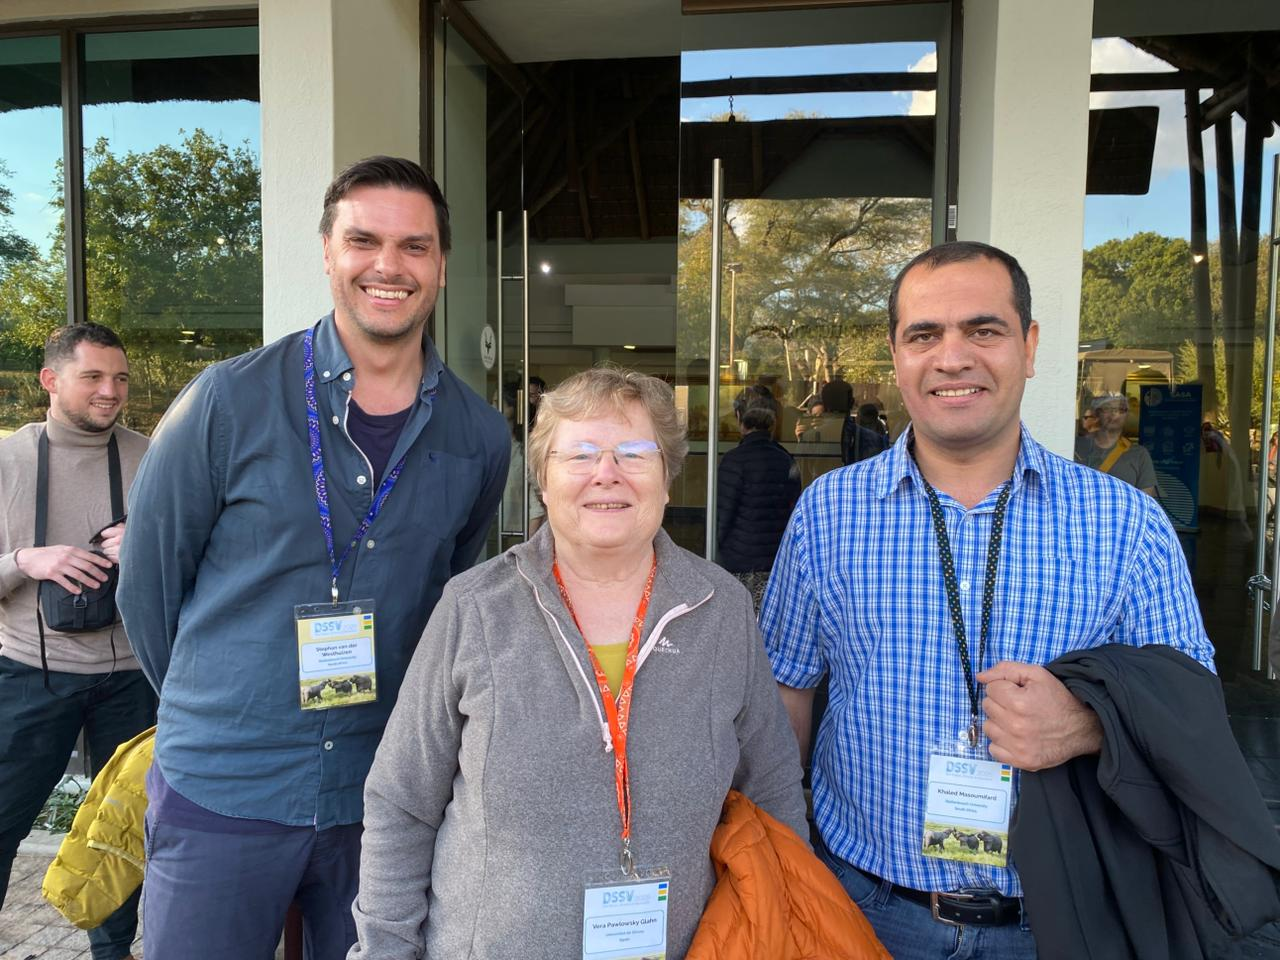
\includegraphics[width=0.4\linewidth]{slides/Vera.jpg}
}
\end{frame}


\begin{frame}{Debates}
\only<1>{
The CoDA school has redefined these principles several times in response to criticism.



        \begin{alertblock}{ (Zier \& Rehder (1998, 2001))}
     They pointed out that even Aitchison’s own earlier work did not strictly satisfy the later CoDA definition of scale invariance.
    \end{alertblock}


        \begin{alertblock}{ (Scealy \& Welsh 2014)}
      The CoDa Principles act as a \textbf{gatekeeping criterion}:
      valid and useful methods have been dismissed simply for not
      conforming to them.
 
      \vspace{0.2cm}
      This is \textbf{unusual, perhaps unique, in statistical
      data analysis}.
    \end{alertblock}
}
\end{frame}



\begin{frame}{One Idea: Transforming to Real Space}





\only<1>{
  \framesubtitle{A transformation $\mathcal{S}^{K-1} \to \mathbb{R}^{K-1}$ unlocks standard inference: regression, PCA, LDA}

  \vspace{0.2cm}
  \renewcommand{\arraystretch}{1.35}
  \setlength{\tabcolsep}{8pt}

  \begin{tabular}{>{\bfseries}l l >{\footnotesize\itshape\color{gray}}l}
    \toprule
    \rowcolor{mainblue}
    \color{white}Method &
    \color{white}Formula &
    \color{white}Reference \\
    \midrule

    \rowcolor{accentblue!20}
    ALR & $\log y_i - \log y_K$ & Aitchison (1982) \\

    \rowcolor{accentblue!20}
    CLR & $\log y_i - K^{-1}\sum_{j=1}^{K} \log y_j$ & Aitchison (1983) \\

    \rowcolor{accentblue!20}
    ILR & $\mathbf{H}\!\left(\log y_i - K^{-1}\sum_{j=1}^{K} \log y_j\right)$ & Egozcue et al.\ (2003) \\

    \midrule
  
    {\normalfont $\alpha$} &
    {\footnotesize $\mathbf{H}[K_\alpha^{-1}(\mathbf{y} \otimes \alpha)]$} &
    Tsagris et al.\ (2011) \\

    {\normalfont BC$_1$} &
    {\footnotesize $\lambda^{-1}\!\left[(y_i / y_K)^\lambda - 1\right]$} &
    Aitchison (2003) \\

    {\normalfont BC$_2$} &
    {\footnotesize $\theta^{-1}(y_i^\theta - 1)$} &
    Greenacre (2010) \\

    {\normalfont Hyper-spherical} &
    {\footnotesize $\arccos\!\left(\dfrac{y_i}{\prod_{j=i+1}^{K} y_j}\right)$} &
    Wang et al.\ (2007) \\

    {\normalfont Square root} &
    {\footnotesize $\sqrt{y_i}$} &
    Stephens (1982) \\

    \bottomrule
  \end{tabular}

  \vspace{0.2cm}
  {\small\textbf{Key:} ALR, CLR, ILR are the most widely used;
  all resolve singularity of $\Sigma_{\mathbf{X}}$ by mapping to unconstrained $\mathbb{R}^{K-1}$.}
}



\end{frame}








\begin{frame}{Machine learning for CoDA}
      \centering
      \vfill
      \textbf{\Large Machine learning for CoDA}
      \vfill
\end{frame}







\begin{frame}{Machine learning: Random Forest}

\begin{itemize}

\item \textbf{Why machine learning?}  
For responses that are compositional: many predictors with complex non-linear patterns that traditional models cannot capture.

\item \textbf{Common approaches}:  
Apply ML models without considering the simplex geometry, or transform data (with log-ratio transformations) to real space (risking distortion and bias).

\item \textbf{Why Random Forests?}  
RFs are flexible and their splitting rules can be easily adapted to respect the simplex structure.

\item PhD of van der Westhuizen (2024) inspired the idea to use tree splitting to account for coDA
\end{itemize}

    
\end{frame}



\begin{frame}{Random Forests framework}
 
\begin{itemize}
   \item[\textcolor{blue}{\large$\blacktriangleright$}]  Given a sample size $n$ and $m$ covariates:
    \[
        \mathbf{X} \in \mathbb{R}^{n \times m} \quad \text{(covariate matrix)}, \qquad
        \mathbf{Y} \in \mathbb{R}^{n \times k} \quad \text{(response matrix)}
    \]
    
  \item[\textcolor{blue}{\large$\blacktriangleright$}]  Each row of \( \mathbf{Y} \) is a compositional vector:
    \[
        Y_{i,j} > 0 \quad \text{for all } i, j, \qquad \sum_{j=1}^k Y_{i,j} = 1
    \]
        
  
     \item[\textcolor{blue}{\large$\blacktriangleright$}] Goal: learn a mapping
    \[
    \mathbf{x} \;\longrightarrow\; \mathbf{y}
    \]
    respecting the simplex geometry
    \vspace{0.8em}

    % \item[\textcolor{blue}{\large$\blacktriangleright$}] Approach: adapt \textbf{random forests} for compositional outputs
    % \vspace{0.8em}

     \item[\textcolor{blue}{\large$\blacktriangleright$}] After training:
    \begin{itemize}
        \item Predict compositional responses for new inputs
        \item Estimate conditional distribution of responses
    \end{itemize}

\end{itemize}
\end{frame}

\begin{frame}{Random Forest: Overview}

A \textbf{Random Forest} is an ensemble of decision trees, each trained on a
bootstrap sample of the data. Key tuning parameters include:

\vspace{0.5em}

\begin{itemize}
    \item \textbf{Number of trees} ($B$): more trees improve stability but increase cost
    \item \textbf{Tree depth} ($d_{\max}$): controls model complexity and overfitting
    \item \textbf{Minimum node size} ($n_{\min}$): minimum observations required to split a node
    \item \textbf{Covariates per split} ($m_{\text{try}}$): number of randomly selected covariates
    considered at each split; typically set to $\sqrt{p}$
\end{itemize}

\end{frame}

\begin{frame}{Random forest: tree}

\centering
\only<1>{

\begin{columns}
    \begin{column}{0.4\linewidth}
    
        \begin{figure}[h]
\centering
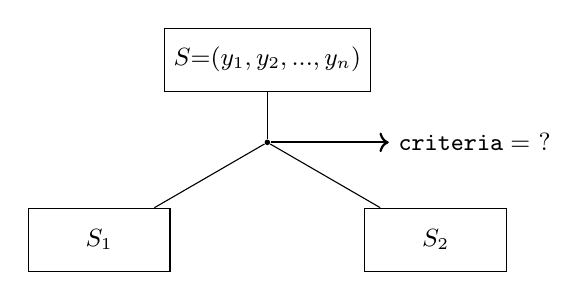
\begin{tikzpicture}[
    node distance=0.8cm,
    box/.style={rectangle, draw, minimum width=1.8cm, minimum height=0.8cm, text centered, font=\small},
    dot/.style={circle, fill=black, minimum size=2pt, inner sep=0pt},
    arrow/.style={->, thick}
]
% Main parent node
\node[box] (parent) {$S$=\\$(y_1, y_2, ..., y_n)$};
% Split point (dot in the middle)
\node[dot, below=0.6cm of parent] (split) {};
% Two child nodes
\node[box, below left=0.8cm and 1.2cm of split] (left) {$S_1$};
\node[box, below right=0.8cm and 1.2cm of split] (right) {$S_2$};
% Connections
\draw (parent) -- (split);
\draw (split) -- (left);
\draw (split) -- (right);
% Loss function arrow and equation
\node[right=1.5cm of split, font=\small] (loss) {$\texttt{criteria} = $ ?};
\draw[arrow] (split) -- (loss);
\end{tikzpicture}

\label{fig:decision_tree_split}
\end{figure}



    \end{column}
\begin{column}{0.6\linewidth}
\vspace{1cm}
$\qquad \qquad$A binary decision tree
\vspace

\resizebox{1\linewidth}{!}{%
        \begin{tikzpicture}[
  level/.style={sibling distance=60mm/#1},
  every node/.style={circle, draw, minimum size=8mm, font=\tiny},
  dots/.style={draw=none, font=\large}
]
\node {Root}
  child {
    node {L1}
    child {
      node {L2}
      child {
        node[dots] {$\vdots$}
      }
      child {
        node[dots] {$\vdots$}
      }
    }
    child {
      node {L2}
      child {
        node[dots] {$\vdots$}
      }
      child {
        node[dots] {$\vdots$}
      }
    }
  }
  child {
    node {R1}
    child {
      node {L2}
      child {
        node[dots] {$\vdots$}
      }
      child {
        node[dots] {$\vdots$}
      }
    }
    child {
      node {L2}
      child {
        node[dots] {$\vdots$}
      }
      child {
        node[dots] {$\vdots$}
      }
    }
  };
\end{tikzpicture}}
    \end{column}

    
\end{columns}


}

\end{frame}






\begin{frame}{}\only<1>{\frametitle{MSE splitting}

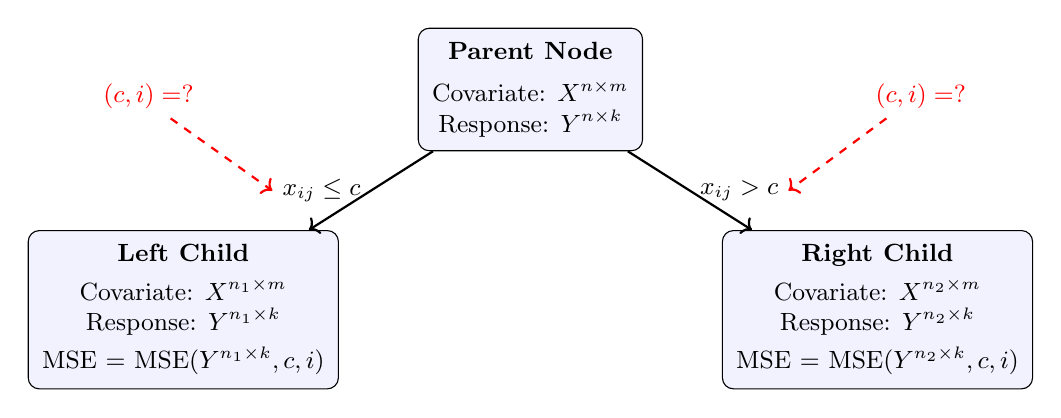
\begin{tikzpicture}[
  node distance=1cm and 1cm,
  every node/.style={font=\small},
  data/.style={rectangle, draw, align=center, fill=blue!5, rounded corners, inner sep=5pt},
  split/.style={->, thick},
  highlight/.style={->, red, thick, dashed}
  ]
  % Parent node
  \node[data] (parent) {
    \textbf{Parent Node} \\[0.15cm]
    Covariate: $X^{n \times m}$ \\ 
    Response: $Y^{n \times k}$
  };
  % Left child
  \node[data, below left=of parent] (left) {
    \textbf{Left Child} \\[0.1cm]
    Covariate: $X^{n_1 \times m}$ \\
    Response: $Y^{n_1 \times k}$ \\[0.1cm]
    MSE = $\text{MSE}(Y^{n_1 \times k},c,i)$
  };
  % Right child
  \node[data, below right=of parent] (right) {
    \textbf{Right Child} \\[0.1cm]
    Covariate: $X^{n_2 \times m}$ \\
    Response: $Y^{n_2 \times k}$ \\[0.1cm]
    MSE = $\text{MSE}(Y^{n_2 \times k},c,i)$
  };
  % Arrows
  \draw[split] (parent) -- node[midway, left] (leftlabel) {$x_{ij} \leq c$} (left);
  \draw[split] (parent) -- node[midway, right] (rightlabel) {$x_{ij} > c$} (right);
  
  % Optimize labels
  \node[red, left] (opt_i) at ([xshift=-1.5cm, yshift=1.2cm]leftlabel) {\textbf{ } $(c,i)=?$};
  \node[red, right] (opt_c) at ([xshift=1.5cm, yshift=1.2cm]rightlabel) {\textbf{} $(c,i)=?$};
  
  % Short highlight arrows from labels to split conditions
  \draw[highlight] (opt_i) -- (leftlabel.west);
  \draw[highlight] (opt_c) -- (rightlabel.east);
\end{tikzpicture}


}
\only<2>{

\frametitle{Split rule}
\begin{columns}[T]

  \column{0.8\textwidth}
 \begin{center}
\renewcommand{\arraystretch}{1.6}
\begin{tabular}{c|c>{\columncolor{purple!20}}cc>{\columncolor{purple!20}}cc|ccc|c}
\textbf{obs} & $x_1$ & \cellcolor{purple!50}$x_2$ & $x_3$ & \cellcolor{purple!20}$x_4$ & $x_5$ & $y_1$ & $y_2$ & $y_3$ & \textbf{child} \\
\hline
\rowcolor{blue!15}
1 & 0.8 & \textbf{1.2} & 3.4 & 0.5 & 2.1 & 0.60 & 0.25 & 0.15 & \textcolor{blue!80!black}{$\leftarrow$ left} \\
\rowcolor{blue!15}
2 & 2.3 & \textbf{2.7} & 1.1 & 4.2 & 0.9 & 0.10 & 0.70 & 0.20 & \textcolor{blue!80!black}{$\leftarrow$ left} \\
\rowcolor{blue!15}
3 & 1.5 & \textbf{3.1} & 2.9 & 1.8 & 3.3 & 0.45 & 0.45 & 0.10 & \textcolor{blue!80!black}{$\leftarrow$ left} \\
\rowcolor{red!15}
4 & 3.9 & \textbf{4.4} & 0.7 & 3.1 & 1.4 & 0.05 & 0.15 & 0.80 & \textcolor{red!80!black}{right $\rightarrow$} \\
\rowcolor{blue!15}
5 & 0.4 & \textbf{2.0} & 4.5 & 2.7 & 5.0 & 0.50 & 0.30 & 0.20 & \textcolor{blue!80!black}{$\leftarrow$ left} \\
\rowcolor{red!15}
6 & 2.1 & \textbf{5.6} & 3.8 & 0.3 & 2.2 & 0.02 & 0.08 & 0.90 & \textcolor{red!80!black}{right $\rightarrow$} \\
\rowcolor{red!15}
7 & 3.3 & \textbf{3.8} & 1.6 & 4.9 & 0.6 & 0.03 & 0.12 & 0.85 & \textcolor{red!80!black}{right $\rightarrow$} \\
\rowcolor{blue!15}
8 & 1.1 & \textbf{1.5} & 2.2 & 1.1 & 4.4 & 0.55 & 0.35 & 0.10 & \textcolor{blue!80!black}{$\leftarrow$ left} \\
\end{tabular}
\end{center}

  \column{0.22\textwidth}
  \vspace{1em}
  \begin{block}{Partition rule}
    Covariate 2: $i=2$ \\ Split value: $c =3.1$\\
    
  \end{block}
  \vspace{0.8em}
  \textcolor{blue!80!black}{\textbf{Left}} \\
  \hspace{0.5em} $x_2 \leq 3.1$ \\[0.2em]
  \hspace{0.5em} obs: 1, 2, 3, 5, 8 \\[0.6em]
  \textcolor{red!80!black}{\textbf{Right}} \\
   \hspace{0.5em} $x_2 > 3.1$ \\
  \hspace{0.5em} obs: 4, 6, 7


\end{columns}
}


\end{frame}




% %--- SLIDE 1: The data ---
% \begin{frame}{Growing a Tree: The Data}
% \begin{columns}[T]

%   \column{0.65\textwidth}
%   \begin{center}
%   \renewcommand{\arraystretch}{1.6}
%   \begin{tabular}{c|ccccc|ccc}
%   \textbf{obs} & $x_1$ & $x_2$ & $x_3$ & $x_4$ & $x_5$ & $y_1$ & $y_2$ & $y_3$ \\
%   \hline
%   1 & 0.8 & 1.2 & 3.4 & 0.5 & 2.1 & 0.60 & 0.25 & 0.15 \\
%   2 & 2.3 & 2.7 & 1.1 & 4.2 & 0.9 & 0.10 & 0.70 & 0.20 \\
%   3 & 1.5 & 3.1 & 2.9 & 1.8 & 3.3 & 0.45 & 0.45 & 0.10 \\
%   4 & 3.9 & 4.4 & 0.7 & 3.1 & 1.4 & 0.05 & 0.15 & 0.80 \\
%   5 & 0.4 & 2.0 & 4.5 & 2.7 & 5.0 & 0.50 & 0.30 & 0.20 \\
%   6 & 2.1 & 5.6 & 3.8 & 0.3 & 2.2 & 0.02 & 0.08 & 0.90 \\
%   7 & 3.3 & 3.8 & 1.6 & 4.9 & 0.6 & 0.03 & 0.12 & 0.85 \\
%   8 & 1.1 & 1.5 & 2.2 & 1.1 & 4.4 & 0.55 & 0.35 & 0.10 \\
%   \end{tabular}
%   \end{center}

%   \column{0.32\textwidth}
%   \vspace{1em}
%   \begin{block}{Setup}
%     Each node holds $n$ observations with $p$ covariates.
%   \end{block}
%   \vspace{0.8em}
%   \textbf{Response} $\mathbf{y}$ is compositional:
%   \[
%     \mathbf{y} = (y_1, y_2, y_3)
%   \]
%   \[
%     y_k \geq 0, \quad \textstyle\sum_k y_k = 1
%   \]
%   \vspace{0.4em}
%   Lives on the simplex $\mathcal{S}^2$.

% \end{columns}
% \end{frame}


% %--- SLIDE 2: Select covariates ---
% \begin{frame}{Step 1 — Select Covariates}
% \begin{columns}[T]

%   \column{0.65\textwidth}
%   \begin{center}
%   \renewcommand{\arraystretch}{1.6}
%   \begin{tabular}{c|c>{\columncolor{purple!20}}cc>{\columncolor{purple!20}}cc|ccc}
%   \textbf{obs} & $x_1$ & \cellcolor{purple!50}$x_2$ & $x_3$ & \cellcolor{purple!50}$x_4$ & $x_5$ & $y_1$ & $y_2$ & $y_3$ \\
%   \hline
%   1 & 0.8 & 1.2 & 3.4 & 0.5 & 2.1 & 0.60 & 0.25 & 0.15 \\
%   2 & 2.3 & 2.7 & 1.1 & 4.2 & 0.9 & 0.10 & 0.70 & 0.20 \\
%   3 & 1.5 & 3.1 & 2.9 & 1.8 & 3.3 & 0.45 & 0.45 & 0.10 \\
%   4 & 3.9 & 4.4 & 0.7 & 3.1 & 1.4 & 0.05 & 0.15 & 0.80 \\
%   5 & 0.4 & 2.0 & 4.5 & 2.7 & 5.0 & 0.50 & 0.30 & 0.20 \\
%   6 & 2.1 & 5.6 & 3.8 & 0.3 & 2.2 & 0.02 & 0.08 & 0.90 \\
%   7 & 3.3 & 3.8 & 1.6 & 4.9 & 0.6 & 0.03 & 0.12 & 0.85 \\
%   8 & 1.1 & 1.5 & 2.2 & 1.1 & 4.4 & 0.55 & 0.35 & 0.10 \\
%   \end{tabular}
%   \end{center}

%   \column{0.32\textwidth}
%   \vspace{1em}
%   \begin{block}{Random subspace}
%     At each node, draw $m \leq p$ covariates at random.
%   \end{block}
%   \vspace{0.8em}
%   \textcolor{purple!80!black}{\textbf{Selected:}} $x_2,\, x_4$
%   \vspace{0.6em}

%   \begin{itemize}[label={\ding{226}}]
%     \item Reduces correlation between trees
%     \item Only \textcolor{purple!80!black}{highlighted columns} are split candidates
%     \item Other columns are ignored at this node
%   \end{itemize}

% \end{columns}
% \end{frame}


% %--- SLIDE 3: Find the best split ---
% \begin{frame}{Step 2 — Find the Best Split}
% \begin{columns}[T]

%   \column{0.72\textwidth}
%   \begin{center}
%   \renewcommand{\arraystretch}{1.6}
%   \begin{tabular}{c|c>{\columncolor{purple!20}}cc>{\columncolor{purple!20}}cc|ccc|c}
%   \textbf{obs} & $x_1$ & \cellcolor{purple!50}$x_2$ & $x_3$ & \cellcolor{purple!20}$x_4$ & $x_5$ & $y_1$ & $y_2$ & $y_3$ & \\
%   \hline
%   \rowcolor{leftblue}
%   1 & 0.8 & \textbf{1.2} & 3.4 & 0.5 & 2.1 & 0.60 & 0.25 & 0.15 & \textcolor{blue!80!black}{$\leftarrow$ left} \\
%   \rowcolor{leftblue}
%   2 & 2.3 & \textbf{2.7} & 1.1 & 4.2 & 0.9 & 0.10 & 0.70 & 0.20 & \textcolor{blue!80!black}{$\leftarrow$ left} \\
%   \rowcolor{leftblue}
%   3 & 1.5 & \textbf{3.1} & 2.9 & 1.8 & 3.3 & 0.45 & 0.45 & 0.10 & \textcolor{blue!80!black}{$\leftarrow$ left} \\
%   \rowcolor{rightred}
%   4 & 3.9 & \textbf{4.4} & 0.7 & 3.1 & 1.4 & 0.05 & 0.15 & 0.80 & \textcolor{red!80!black}{right $\rightarrow$} \\
%   \rowcolor{leftblue}
%   5 & 0.4 & \textbf{2.0} & 4.5 & 2.7 & 5.0 & 0.50 & 0.30 & 0.20 & \textcolor{blue!80!black}{$\leftarrow$ left} \\
%   \rowcolor{rightred}
%   6 & 2.1 & \textbf{5.6} & 3.8 & 0.3 & 2.2 & 0.02 & 0.08 & 0.90 & \textcolor{red!80!black}{right $\rightarrow$} \\
%   \rowcolor{rightred}
%   7 & 3.3 & \textbf{3.8} & 1.6 & 4.9 & 0.6 & 0.03 & 0.12 & 0.85 & \textcolor{red!80!black}{right $\rightarrow$} \\
%   \rowcolor{leftblue}
%   8 & 1.1 & \textbf{1.5} & 2.2 & 1.1 & 4.4 & 0.55 & 0.35 & 0.10 & \textcolor{blue!80!black}{$\leftarrow$ left} \\
%   \end{tabular}
%   \end{center}

%   \column{0.25\textwidth}
%   \vspace{1em}
%   \begin{block}{Partition rule}
%     \textcolor{purple!80!black}{Best:} $x_2 \leq 3.5$
%   \end{block}
%   \vspace{0.8em}
%   \textcolor{blue!80!black}{\textbf{Left}} \hfill $x_2 \leq 3.5$\\[0.2em]
%   \hspace{0.5em} obs: 1,2,3,5,8 \\[0.6em]
%   \textcolor{red!80!black}{\textbf{Right}} \hfill $x_2 > 3.5$ \\[0.2em]
%   \hspace{0.5em} obs: 4,6,7
%   \vspace{0.6em}



% \end{columns}
% \end{frame}





\begin{frame}{}\only<1>{\frametitle{MSE splitting}

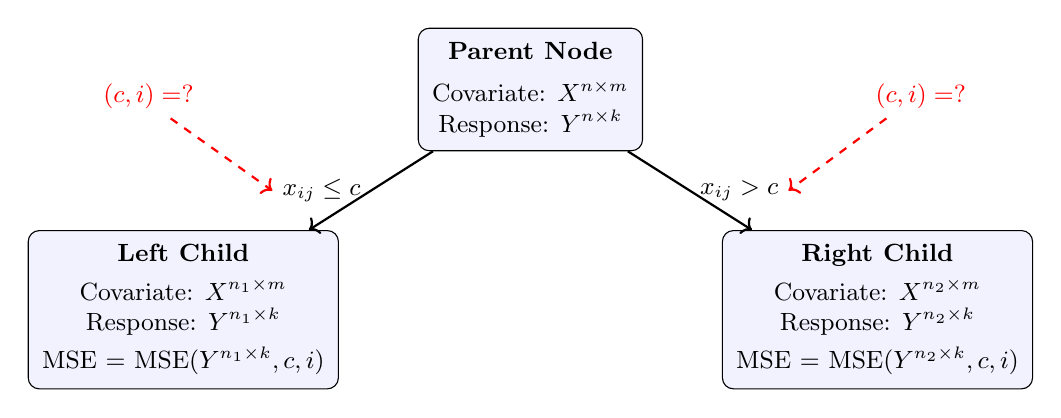
\begin{tikzpicture}[
  node distance=1cm and 1cm,
  every node/.style={font=\small},
  data/.style={rectangle, draw, align=center, fill=blue!5, rounded corners, inner sep=5pt},
  split/.style={->, thick},
  highlight/.style={->, red, thick, dashed}
  ]
  % Parent node
  \node[data] (parent) {
    \textbf{Parent Node} \\[0.15cm]
    Covariate: $X^{n \times m}$ \\ 
    Response: $Y^{n \times k}$
  };
  % Left child
  \node[data, below left=of parent] (left) {
    \textbf{Left Child} \\[0.1cm]
    Covariate: $X^{n_1 \times m}$ \\
    Response: $Y^{n_1 \times k}$ \\[0.1cm]
    MSE = $\text{MSE}(Y^{n_1 \times k},c,i)$
  };
  % Right child
  \node[data, below right=of parent] (right) {
    \textbf{Right Child} \\[0.1cm]
    Covariate: $X^{n_2 \times m}$ \\
    Response: $Y^{n_2 \times k}$ \\[0.1cm]
    MSE = $\text{MSE}(Y^{n_2 \times k},c,i)$
  };
  % Arrows
  \draw[split] (parent) -- node[midway, left] (leftlabel) {$x_{ij} \leq c$} (left);
  \draw[split] (parent) -- node[midway, right] (rightlabel) {$x_{ij} > c$} (right);
  
  % Optimize labels
  \node[red, left] (opt_i) at ([xshift=-1.5cm, yshift=1.2cm]leftlabel) {\textbf{ } $(c,i)=?$};
  \node[red, right] (opt_c) at ([xshift=1.5cm, yshift=1.2cm]rightlabel) {\textbf{} $(c,i)=?$};
  
  % Short highlight arrows from labels to split conditions
  \draw[highlight] (opt_i) -- (leftlabel.west);
  \draw[highlight] (opt_c) -- (rightlabel.east);
\end{tikzpicture}

\begin{align*}
    
(c^*, i^*) 
&=& \operatorname{argmin}_{i,c} \left( \text{MSE}(Y^{n_1 \times k},c,i) + \text{MSE}(Y^{n_2 \times k},c,i) \right)
\\
&=& \arg\min_{c,j} 
\left\{\frac{n_1(c,j)}{n}
\sum_{m=1}^k \sum_{i=1}^{n_1(c,j)} (y_{im}-\bar{y}_{m}^{n_1(c,j)})^2
+
\frac{n_2(c,j)}{n}
\sum_{m=1}^k \sum_{i=1}^{n_2(c,j)} (y_{im}-\bar{y}_{m}^{n_2(c,j)})^2
\right\}.
\end{align*}

}



\only<2>{ \frametitle{MSE splitting}

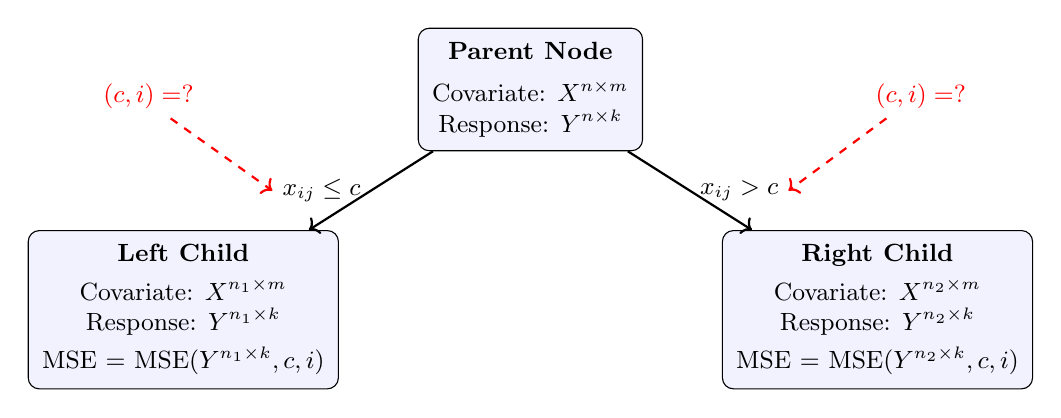
\begin{tikzpicture}[
  node distance=1cm and 1cm,
  every node/.style={font=\small},
  data/.style={rectangle, draw, align=center, fill=blue!5, rounded corners, inner sep=5pt},
  split/.style={->, thick},
  highlight/.style={->, red, thick, dashed}
  ]
  % Parent node
  \node[data] (parent) {
    \textbf{Parent Node} \\[0.15cm]
    Covariate: $X^{n \times m}$ \\ 
    Response: $Y^{n \times k}$
  };
  % Left child
  \node[data, below left=of parent] (left) {
    \textbf{Left Child} \\[0.1cm]
    Covariate: $X^{n_1 \times m}$ \\
    Response: $Y^{n_1 \times k}$ \\[0.1cm]
    MSE = $\text{MSE}(Y^{n_1 \times k},c,i)$
  };
  % Right child
  \node[data, below right=of parent] (right) {
    \textbf{Right Child} \\[0.1cm]
    Covariate: $X^{n_2 \times m}$ \\
    Response: $Y^{n_2 \times k}$ \\[0.1cm]
    MSE = $\text{MSE}(Y^{n_2 \times k},c,i)$
  };
  % Arrows
  \draw[split] (parent) -- node[midway, left] (leftlabel) {$x_{ij} \leq c$} (left);
  \draw[split] (parent) -- node[midway, right] (rightlabel) {$x_{ij} > c$} (right);
  
  % Optimize labels
  \node[red, left] (opt_i) at ([xshift=-1.5cm, yshift=1.2cm]leftlabel) {\textbf{ } $(c,i)=?$};
  \node[red, right] (opt_c) at ([xshift=1.5cm, yshift=1.2cm]rightlabel) {\textbf{} $(c,i)=?$};
  
  % Short highlight arrows from labels to split conditions
  \draw[highlight] (opt_i) -- (leftlabel.west);
  \draw[highlight] (opt_c) -- (rightlabel.east);
\end{tikzpicture}
\begin{itemize}
    \item 
MSE does not account for the simplex constraint.

\item 
\[V(X_i)=\frac{E(X_i)\left(1-E(X_i)\right)}{\alpha_0+1}\]
\end{itemize}

}

\end{frame}







\begin{frame}
\only<1>{
\frametitle{Dirichlet distribution}


\vspace{1em}

\begin{center}
\colorbox{green!10}{\parbox{0.95\textwidth}{
\begin{center}
\resizebox{\linewidth}{!}{%
\[
    f_{\mathbf{Z}}((z_1,\ldots,z_k); \boldsymbol{\alpha}) = \frac{\Gamma( \alpha_0)}{\prod_{i=1}^k \Gamma(\alpha_i)} \prod_{i=1}^k z_i^{\alpha_i - 1},
\quad  z_i \in [0, 1], \quad \sum_{i=1}^k z_i = 1,
\]
}
\end{center}
}}
\end{center}

\vspace{1.5em}

\begin{itemize}[itemsep=0.8em]


\item[\textcolor{blue}{\large$\blacktriangleright$}] The sum-constant requirement of the simplex is satisfied under the Dirichlet distribution.

\item[\textcolor{blue}{\large$\blacktriangleright$}] \textbf{Extensions available:} Zero-inflated Dirichlet and Kummer–Dirichlet
\end{itemize}
}

\end{frame}


\begin{frame}
\only<1>{\frametitle{Dirichlet log-likelihood splitting}

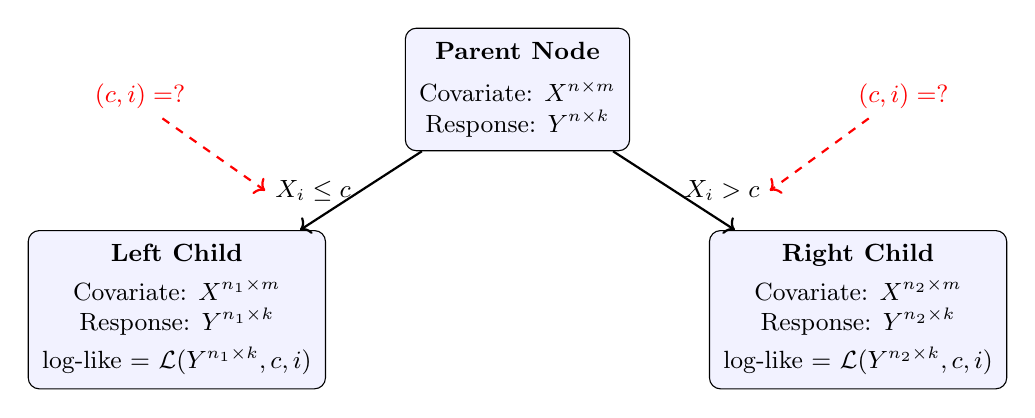
\begin{tikzpicture}[
  node distance=1cm and 1cm,
  every node/.style={font=\small},
  data/.style={rectangle, draw, align=center, fill=blue!5, rounded corners, inner sep=5pt},
  split/.style={->, thick},
  highlight/.style={->, red, thick, dashed}
  ]
  % Parent node
  \node[data] (parent) {
    \textbf{Parent Node} \\[0.15cm]
    Covariate: $X^{n \times m}$ \\ 
    Response: $Y^{n \times k}$
  };
  % Left child
  \node[data, below left=of parent] (left) {
    \textbf{Left Child} \\[0.1cm]
    Covariate: $X^{n_1 \times m}$ \\
    Response: $Y^{n_1 \times k}$ \\[0.1cm]
     log-like = $\mathcal{L}(Y^{n_1 \times k},c,i)$
  };
  % Right child
  \node[data, below right=of parent] (right) {
    \textbf{Right Child} \\[0.1cm]
    Covariate: $X^{n_2 \times m}$ \\
    Response: $Y^{n_2 \times k}$ \\[0.1cm]
     log-like = $\mathcal{L}(Y^{n_2 \times k},c,i)$
  };
  % Arrows
  \draw[split] (parent) -- node[midway, left] (leftlabel) {$X_{i} \leq c$} (left);
  \draw[split] (parent) -- node[midway, right] (rightlabel) {$X_{i} > c$} (right);
  
  % Optimize labels
  \node[red, left] (opt_i) at ([xshift=-1.5cm, yshift=1.2cm]leftlabel) {\textbf{ } $(c,i)=?$};
  \node[red, right] (opt_c) at ([xshift=1.5cm, yshift=1.2cm]rightlabel) {\textbf{} $(c,i)=?$};
  
  % Short highlight arrows from labels to split conditions
  \draw[highlight] (opt_i) -- (leftlabel.west);
  \draw[highlight] (opt_c) -- (rightlabel.east);
\end{tikzpicture}
\[
(c^*, i^*) = \operatorname{argmax}_{i,c} \left( \max_{\boldsymbol{\alpha}} \mathcal{L}(Y^{n_1 \times k},c,i) + \max_{\boldsymbol{\alpha}} \mathcal{L}(Y^{n_2 \times k},c,i) \right)
\]
}
\end{frame}

\begin{frame}{Prediction based on DirichletRF}

    
\begin{columns}[T]

% Left column - Graph
\begin{column}{0.45\textwidth}
\centering
\begin{tikzpicture}[
    node/.style={ellipse, draw, minimum width=1.2cm, minimum height=0.8cm, thick},
    leaf/.style={rectangle, draw, minimum width=1.8cm, minimum height=0.6cm, thick},
    arrow/.style={->, thick, blue},
    scale=0.75,
    every node/.style={transform shape}
]

% Root node
\node[node] (root) at (0,0) {};

% Level 1
\node[node] (n1) at (-2,-2) {};
\node (dots1) at (1,-2) {\vdots};

% Level 2
\node (dots2) at (-3,-3.5) {\vdots};
\node[node] (n2) at (-1,-4) {};

% Level 3
\node (dots3) at (-2.5,-5.5) {\vdots};
\node[node] (n3) at (0,-6) {};

% Level 4
\node (dots4) at (1,-7.5) {\vdots};
\node[leaf] (leaf) at (-1,-8) {$\{y_1, y_2, \ldots, y_{n_t^'}\}$};

% Arrows - traversal path highlighted
\draw[arrow, line width=1.5pt] (root) -- (n1);
\draw[arrow, dashed] (root) -- (dots1);
\draw[arrow, dashed] (n1) -- (dots2);
\draw[arrow, line width=1.5pt] (n1) -- (n2);
\draw[arrow, dashed] (n2) -- (dots3);
\draw[arrow, line width=1.5pt] (n2) -- (n3);
\draw[arrow, line width=1.5pt] (n3) -- (leaf);
\draw[arrow, dashed] (n3) -- (dots4);

\end{tikzpicture}
\end{column}

% Right column - Explanation
\begin{column}{0.52\textwidth}
\small

\textbf{Process:}
\begin{itemize}
\item[1)] Start at root node
    \item[2)] Traverse tree based on decision rules
    \item[3)] Reach terminal node with observations
\end{itemize}

\vspace{0.4cm}

\textbf{Default Approach:}
\begin{itemize}
    \item Mean: $\hat{y} = \frac{1}{n_t^'}\sum_{i=1}^{n_t^{'}} y_i$
    \item Expectation: $\text{E}(Y_i) = \frac{\hat{\alpha}_i}{\sum_{j+1}^k\hat{\alpha}_i}$
    \item Random Forest: average across trees
\end{itemize}

\vspace{0.4cm}

\textbf{Distributional Approach:}
\begin{itemize}
    \item Collect terminal nodes from all trees
    \item Construct empirical probability function
\end{itemize}

\end{column}

\end{columns}

\end{frame}










%-----------------------------------------------------------------------------
%===================================================
% Comparison Results


\begin{frame}{Comparison Results}
      \centering
      \vfill
      \textbf{\Large Comparison Results}
      \vfill
\end{frame}

\begin{frame}{Performance Evaluation and Transformations}

To evaluate DirichletRF's performance, we compare it with two alternative approaches:
\begin{itemize}
    \item[1)] \textbf{ILR-RF:} A Random Forest model based on log-ratio transformations. 
    The compositional data are first transformed into the ILR
    space. Then, a standard Random Forest is applied to the transformed data, and 
    finally, the predictions are mapped back to the simplex for interpretation.

    \item[2)] \textbf{Dirichlet Regression:} A parametric approach that, 
    works directly on the simplex without requiring any transformation.
\end{itemize}

\end{frame}




\begin{frame}{Evaluation Metrics}

To compare these models, we used  the Aitchison Distance.
\vspace{0.2cm}
\[
AC = \frac{1}{n} \sum_{i=1}^n \sqrt{\sum_{j=1}^k \left(\log\frac{Y_{ij}}{g(\mathbf{Y}_i)} - \log\frac{\hat{Y}_{ij}}{g(\hat{\mathbf{Y}}_i)}\right)^2},
\]
\[
\text{where} \quad g(\mathbf{Y}_i) = \left(\prod_{j=1}^k Y_{ij}\right)^{1/k}
\]


\vspace{0.3cm}
\textbf{Interpretation:} Lower values for this metric indicate better predictive accuracy.
\end{frame}








\begin{frame}{}

    \only<1>{
  
    \textbf{Simple structure simulations}: We use a simple dataset with $3$ Covariate variables, $X_1,X_1, X_{3}$ and with a $3$-dimensional response, $(Y_1,\,Y_2,\,Y_3)$ such that $Y_1+Y_2+Y_3 = 1$. The response is assumed to follow a Dirichlet distribution with the following parameters:
\[
\alpha_1 = 1 + 2 X_1,\quad \alpha_2 =1 + 0.5 X_2,\quad \alpha_3 = 1 + X_3.
\]
\[
(Y_1,\,Y_2,\,Y_3)\sim Dirichlet(\alpha_1,\alpha_2,\alpha_3)
\]
    }
    \only<2>{
      
Dirichlet Regression performed better than the other models. This result makes sense, because the data was generated using a Dirichlet distribution with a linear structure.


But, Dirichlet Random Forest does not perform well in this case — in fact, it gives the worst performance in terms of Aitchison Distance and RMSE.
\begin{table}[htbp]
\centering
\small 
\begin{tabular}{|l|l|c|c|}
\hline
$N$ & Model & Aitchison Distance & Train-Test \\
\hline
\multirow{3}{*}{200} 
    & ILR-RF & 1.303 (0.143) & 0.686 \\
    & \textcolor{blue}{Dirichlet Regression} & \textcolor{blue}{\textbf{1.233} (0.139)} & \textcolor{blue}{\textbf{0.030}} \\
    & \texttt{Dirichlet-RF} & 1.451 (0.153) & 0.600 \\
\hline
\multirow{3}{*}{500}
    & ILR-RF & 1.284 (0.077) & 0.685 \\
    & \textcolor{blue}{Dirichlet Regression} & \textcolor{blue}{\textbf{1.234} (0.078)} & \textcolor{blue}{\textbf{0.035}} \\
    & \texttt{Dirichlet-RF} & 1.450 (0.077) & 0.616 \\
\hline
\multirow{3}{*}{2000}
    & ILR-RF & 1.252 (0.032) & 0.654 \\
    & \textcolor{blue}{Dirichlet Regression} & \textcolor{blue}{\textbf{1.209} (0.032)} & \textcolor{blue}{\textbf{0.006}} \\
    & \texttt{Dirichlet-RF} & 1.431 (0.041) & 0.596 \\
\hline
\end{tabular}
\caption{Values represent the means and (standard deviations) of the metrics for test datasets. Train-Test Diff represents the absolute difference between train and test Aitchison Distance, indicating model generalisation capability.}
\label{tab:performance-comparison1}
\end{table}}

    \only<3>{
    	    

    
    Complex structure synthetic simulations: The dataset consisted of 10 predictor variables \((X_1, \ldots, X_{10})\), with only the first three variables \((X_1, X_2, X_3)\) being truly informative for predicting the compositional response. The three-component compositional response vector $\mathbf{Y} = (Y_1,Y_2,Y_3)$ was constructed through complex non-linear transformations of the informative Covariates. }
    \end{frame}
\begin{frame}
    \only<1>{

\begin{columns}
\begin{column}{0.5\linewidth}

% where \( \mathcal{N}(\mu_i, 0.5^2) \) represents a normally distributed random variable with mean \( \mu_i \) and standard deviation \( 0.5 \), and \( \epsilon \) is a small positive constant ensuring non-negativity.  
% The compositional response variables \( Y_1, Y_2, Y_3 \) are then obtained via the normalisation:
We generate the variables \( Z_1, Z_2, Z_3 \) as follows:  
\[
Z_i = \max(\epsilon, \mathcal{N}(\mu_i, 0.5)), \quad 
\]
\[
Y_i = \frac{Z_i}{Z_1 + Z_2 + Z_3}, \quad  i = 1,2,3.
\]
% This transformation ensures that \( (Y_1, Y_2, Y_3) \) lies within the unit simplex, preserving the compositional structure of the data.
\end{column}
		\begin{column}{0.5\linewidth}

\begin{align*}
\mu_{1j} &= g(2(1 + \sin(x_{1j}))+x_{2j}^3) \\
\mu_{2j} &= g(1 + 2.5\exp(x_{3j})+x_{1j}^2) \\
\mu_{3j} &= g(1 + (1+x_{2j})^2+x_{3j}^4)
\end{align*}

\end{column}

\end{columns}

Where
\[
g(x_{ij}) =
\begin{cases} 
    2, & x_{ij} < \text{Quantile}(x_i, 0.3) \\
    3, & \text{Quantile}(x_i, 0.3) \leq x_{ij} <\text{Quantile}(x_i, 0.6) \\
    4, & \text{Quantile}(x, 0.6) \leq x_{ij} \leq \text{Quantile}(x_i, 0.8) \\
    1, & x_i > \text{Quantile}(x_i, 0.8)
\end{cases}
\]

}
\end{frame}
\begin{frame}
\only<1>{

In this complex scenario, the results are reversed. Our Dirichlet-RF is now the best model, and Dirichlet Regression is the worst.
\begin{table}[htbp]
\centering
\small 
\begin{tabular}{|l|l|c|c|}
\hline
$N$ & Model & Aitchison Distance & Train-Test \\
\hline
\multirow{3}{*}{200} 
    & ILR-RF & 0.670 (0.151) & 0.364 \\
    & Dirichlet Regression & 0.826 (0.155) & 0.068 \\
    & \textcolor{blue}{\texttt{Dirichlet-RF}} & \textcolor{blue}{\textbf{0.659} (0.152)} & \textcolor{blue}{0.221} \\
\hline
\multirow{3}{*}{500}
    & ILR-RF & 0.618 (0.072) & 0.334 \\
    & Dirichlet Regression & 0.790 (0.075) & 0.029 \\
    & \textcolor{blue}{\texttt{Dirichlet-RF}} & \textcolor{blue}{\textbf{0.606} (0.068)} & \textcolor{blue}{0.201} \\
\hline
\multirow{3}{*}{2000}
    & ILR-RF & 0.557 (0.044) & 0.301 \\
    & Dirichlet Regression & 0.785 (0.044) & 0.016 \\
    & \textcolor{blue}{\texttt{Dirichlet-RF}} & \textcolor{blue}{\textbf{0.544} (0.044)} & \textcolor{blue}{0.178} \\
\hline
\end{tabular}
\caption{Train-Test Diff represents the absolute difference between train and test Aitchison Distance.}
\label{tab:performance-comparison}
\end{table}
}
\end{frame}



\begin{frame}{Learning Curve}
\only<1>{


\begin{figure}
    \centering
    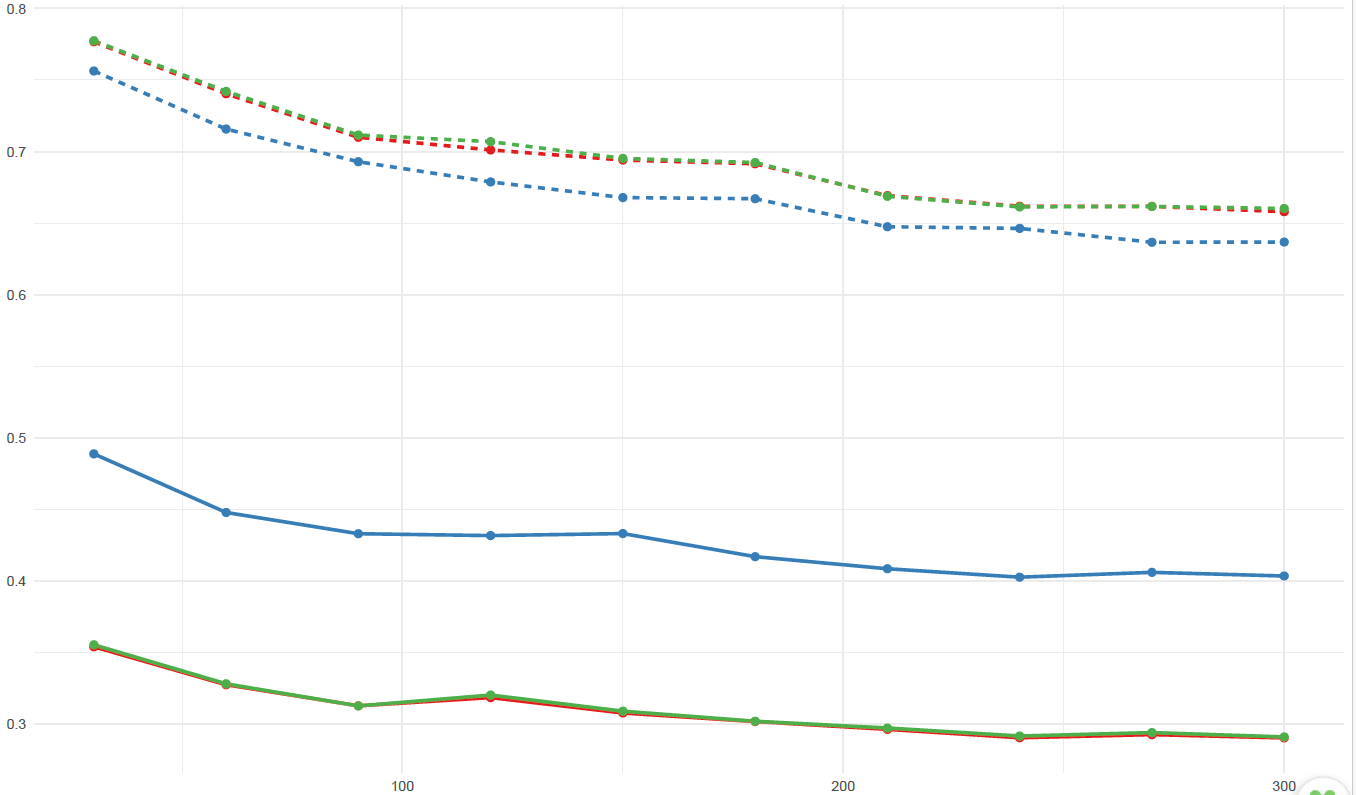
\includegraphics[width=0.75\linewidth]{Learning_curve.png}
    \caption{Aitchison distance as a function of training sample size for all three 
    Random Forest models.}
    \label{fig:enter-label}
\end{figure}
}
\end{frame}




% \begin{frame}
% \only<1>{
% \note{I am not sure to include this slide:

% And for further evaluation of \texttt{Dirichlet-RF}, we also looked at its performance in terms of covariate selection.

% Here, you can see how often each covariate was selected for splitting across all trees, and how much, on average, it contributed to increasing the log-likelihood.

% As I mentioned earlier, only three of the variables were informative — and \texttt{Dirichlet-RF} was able to clearly identify them with high importance.}
% \begin{table}[htbp]
% \centering
% \begin{tabular}{|c|c|c|}
% \hline
% \textbf{Covariate} & \small{Log-Likelihood Importance} & \small{Frequency-Based Importance} \\
% \hline
% \textcolor{blue}{$X_1$} & \textcolor{blue}{225.039} & \textcolor{blue}{14} \\
% \textcolor{blue}{$X_2$} & \textcolor{blue}{303.618} & \textcolor{blue}{21} \\
% \textcolor{blue}{$X_3$} & \textcolor{blue}{272.036} & \textcolor{blue}{19} \\
% \textcolor{red}{$X_4$} & \textcolor{red}{16.839}  & \textcolor{red}{2}  \\
% \textcolor{red}{$X_5$} & \textcolor{red}{9.972}   & \textcolor{red}{2}  \\
% \textcolor{red}{$X_6$} & \textcolor{red}{15.649}  & \textcolor{red}{3}  \\
% \textcolor{red}{$X_7$} & \textcolor{red}{0}   & \textcolor{red}{0}  \\
% \textcolor{red}{$X_8$} & \textcolor{red}{40.240}  & \textcolor{red}{6}  \\
% \textcolor{red}{$X_9$} & \textcolor{red}{5.369}   & \textcolor{red}{1}  \\
% \textcolor{red}{$X_{10}$} & \textcolor{red}{23.295}  & \textcolor{red}{3}  \\
% \hline
% \end{tabular}
% \caption{Variable importance scores based on log-likelihood improvement and selection frequency, averaged across all trees in the \texttt{Dirichlet-RF}.}

% \label{tab:variable-importance}
% \end{table}

% }
% \end{frame}






\begin{frame}{Implementation \& Code Access}
\note{This model was developed in Julia, and the full code is available on GitHub at the link provided.

We chose Julia mainly because of its strong computational performance. Implementing the model directly in R or Python would be much slower.

However, if you're working in R or Python, you can still use the model by calling the Julia functions from those languages.
We've included clear instructions in the repository, especially on how to connect Julia with R.

We're also planning to develop an R package with a C++ backend, which we hope to submit to CRAN, so the model will be even easier for R users to access.}
\vspace{1em}

\begin{itemize}[itemsep=1em]
\item[\textcolor{blue}{\large$\blacktriangleright$}] Model developed in \textbf{Julia} for computational efficiency

\item[\textcolor{blue}{\large$\blacktriangleright$}] Code available on \href{https://github.com/Xaleed/DirichletRandomForestJulia.git}{\textcolor{blue}{\textbf{GitHub}}}:

\textcolor{blue}{\small{https://github.com/Xaleed/DirichletRandomForestJulia.git}}
  \begin{center}

    \qrcode{https://github.com/Xaleed/DirichletRandomForestJulia.git}
 \end{center}



\end{itemize}

\vspace{1.5em}

\end{frame}


\begin{frame}{Alternative to MLE}
    \only<1>{
    \begin{block}{}
        One simple way to address this issue is to use the method of moments (MoM) as an alternative to maximum likelihood estimation (MLE). MoM gives an approximate solution but is much faster to compute.
    \end{block}
     \begin{block}{}
        We can also combine both approaches — instead of using MoM in all nodes, we can selectively apply it only in nodes where we expect its results to be close to MLE. This helps reduce computation while still keeping good accuracy.
    \end{block}
            \resizebox{0.65\linewidth}{!}{%

\begin{table}[htbp]
\centering

\begin{tabular}{|l|c|c|c|c|}
\hline
\multirow{2}{*}{Metric} & \multicolumn{2}{c|}{MLE} & \multicolumn{2}{c|}{MoM} \\
\cline{2-5}
 & (Train) & (Test) & (Train) & (Test) \\
\hline
Aitchison Distance & 0.3901 & 0.7391 & 0.4068 & 0.7457 \\
\hline
\end{tabular}
\end{table}}



}
\end{frame}



% \begin{frame}[plain]
% % \begin{center}
% %    
\includegraphics[width=5cm]{logo.png} % Optional logo
% %    \end{center}
%   \begin{center}
%       \vspace{2cm}

%     {\Huge \textbf{Thank You!} \par}
%     % \vspace{1cm}
%     % {\Large Questions or Comments? \par}
%     \vspace{1cm}
   
    
%     \qrcode{https://github.com/Xaleed/DirichletRandomForestJulia.git}
%    % \texttt{khaledmasoumifard@sun.ac.za}
%   \end{center}
% \end{frame}






%
{
  \setbeamercolor{page number in head/foot}{fg=background canvas.bg}
  \begin{frame}
    \begin{tikzpicture}[remember picture, overlay]
      \node[anchor=north west, xshift=1em, yshift=-1em] at (current page.north west) {
        
\includegraphics[width=3cm]{logo.png}
      };
    \end{tikzpicture}

    \titlepage


      \begin{center}
    %    
\includegraphics[width=0.15\linewidth]{slides/DirichletRF.jpg}
    \qrcode[height=2.8cm]{https://github.com/Xaleed/DirichletRF.git}

    \vspace{0.1cm}

    {\small GitHub repository}

  \end{center}
  \end{frame}
}


\begin{frame}{What is This Talk About?}
% \note{
% Good morning, and thank you for joining this talk. It is about developing DDRF, which is part of my postdoc project at Stellenbosch University, in collaboration with Stephan and Professor Lubbe.


% In a nutshell, I’ll shortly refer what composistional data is? I will explain why is it reasonable to develop a random forest model for composiational data?
% I will some comparison result?}

\vspace{2em}

\nocite{In a nutshell, I will first talk about what compositional data are. Then, I will give a short literature review, including a brief history of compositional data and how this field developed. After that, I will move to the machine learning part, with a particular focus on Random Forests, and explain the model that we developed. I will also present some comparative results, where I compare our model with existing approaches. Finally, I will briefly introduce the R package that we developed.}

\vspace{1.5em}
\begin{itemize}
 
  \item[\textcolor{blue}{\large$\blacktriangleright$}] \textbf{Compositional data} -- Key characteristics and modeling challenges
    \vspace{1em}

    
  \item[\textcolor{blue}{\large$\blacktriangleright$}] \textbf{Machine learning: Random Forest} Modeling complex relationships
    \vspace{1em}
     \item[\textcolor{blue}{\large$\blacktriangleright$}] \textbf{ Dirichlet Random Forest model} -- Introduction and motivation
  \vspace{1em}

  \item[\textcolor{blue}{\large$\blacktriangleright$}] \textbf{Comparison results} -- Evaluating model performance
    \vspace{1em}
  \item[\textcolor{blue}{\large$\blacktriangleright$}] \textbf{
  DirichletRF R package}
\end{itemize}


\vspace{2em}

\end{frame}

%

\begin{frame}{Compositional data}
\only<1>{
\note{
IFirst of all we should know what simplex space is, I will frequently refer to simplex space. 
A simplex space is  collection of vectors with non-negative values that always sum to a constant.
This space is known as the \emph{simplex} and it is common to set \( k = 1 \).
We refer to data from this space as \emph{compositional data}.

The problem I'm going to talk about is how can we apply a random forest to this space and why is this important?
}


\vspace{1em}

A simplex is a convex space of all vectors with non-negative components that sum to a constant. 



\begin{center}
\colorbox{blue!10}{\parbox{0.8\textwidth}{
\begin{center}
\[
S^c_k = \left\{ (y_1, \dots, y_k)^\top \in \mathbb{R}^k \,\middle|\, y_i \geq 0, \ \sum_{i=1}^k y_i = \textcolor{blue}{c} \right\}
\]
\end{center}
}}
\end{center}



 It is common to set \(  \textcolor{blue}{c = 1} \). We refer to data from this space as \emph{compositional data}.
 

}



\only<2>{

\textbf{A practical view of compositional data}

\vspace{0.3cm}

Let $\mathbf{Y} = (Y_1, Y_2, \dots, Y_K)$ be a vector with positive components.

\vspace{0.3cm}

The compositional transformation is defined as:
\[
\mathbf{S} =
\left(
\frac{Y_1}{\sum_{i=1}^K Y_i}, \dots,
\frac{Y_K}{\sum_{i=1}^K Y_i}
\right)
\]

\vspace{0.3cm}

This vector lies in the simplex space.

\vspace{0.5cm}

However, in this transformation we lose information about the \textbf{absolute scale}, and we cannot uniquely recover the original vector.

But we preserve the \textbf{relative information}.
In particular, for any two components $i$ and $j$:
\[
\frac{Y_i}{Y_j} = \frac{S_i}{S_j}
\]


\note{
Improved spoken version

We can also define compositional data in a more practical way.

Suppose we have a vector with non-negative components and no other restrictions.

If we divide each component by the total sum, we obtain a new vector that belongs to the simplex space.

This new vector is a compositional representation of the original data.

An important point is that we cannot recover the original vector uniquely from its compositional form.

In this transformation, we lose information about the absolute scale of the data.

However, what we can fully preserve is the relative information.

In particular, the ratios between components remain exactly the same after normalization.

So for any two components, the ratio is identical in both representations.

It is commonly assumed in this field that absolute values are not important.

The only meaningful information in compositional data is the relative information between components.
}


}

% \only<3>{
% \vspace{.2cm}
%    \textbf{Example}: consider 
% \(
% \mathbf{Y} = (2000, 3000, 5000),
% \)
% which represents the amount of money (in dollars) allocated to \textit{stocks}, \textit{bonds}, and \textit{cash} in an investment portfolio.  

% Then the following vector is a compositional data:
% \begin{align*}
% \scalebox{1.2}{$\left(\frac{2000}{2000+3000+5000},\;\frac{3000}{2000+3000+5000},\;\frac{5000}{2000+3000+5000}\right)$} = (0.2, 0.3, 0.5)
% \end{align*}

% \medskip

% Multiply by 100:
% \[
% 100 \cdot \mathbf{s}(\mathbf{Y}) = (20, 30, 50)
% \]

% \medskip

% Same proportions, different scale (percentages).
% \note{
% Here we see a portfolio allocation example.

% After normalization, we obtain proportions of total investment.

% Multiplying by 100 expresses them as percentages, which are more intuitive in finance.

% The relative allocation (20\%, 30\%, 50\%) remains unchanged regardless of the total invested amount.
% }
% }


\only<3>{
\note{Confirm:In this slide, consider a job application pool of 50 applicants. Among them, 10 have a mathematics background, 15 have a statistics background, and 25 have a computer science background.

If we normalize this vector by dividing each component by the total sum, we obtain a compositional vector.

Each component corresponds to the proportion of applicants with a different academic background.

By multiplying this vector by 100, we obtain percentages. For example, 20% of the applicants have a mathematics background.

The important point is that the information remains the same, but the scale changes—from proportions to percentages.

In general, multiplying a compositional vector by any positive constant does not change the relative information; it only changes the scale.

Now, this simple normalization step looks simple, but it has a very important statistical consequence.
}

Consider a job application pool of $50$ applicants classified by academic background.
\vspace{0.3cm}

\begin{columns}
    \begin{column}{0.4\textwidth}
        \[
        \mathbf{Y} = (10, 15, 25)
        \]
    \end{column}
    \begin{column}{0.5\textwidth}
        \begin{tabular}{lr}
            Mathematics & 10 \\
            Statistics  & 15 \\
            Computer Science & 25 \\
        \end{tabular}
    \end{column}
\end{columns}

\vspace{0.3cm}
We normalize this vector to obtain a compositional representation:
\vspace{0.2cm}

\begin{columns}
    \begin{column}{0.5\textwidth}
        \[
        \mathbf{s}(\mathbf{Y}) = \left(\frac{10}{50}, \frac{15}{50}, \frac{25}{50}\right)
        \]
    \end{column}
    \begin{column}{0.4\textwidth}
        \[
        = (0.2, 0.3, 0.5)
        \]
        Interpreted as proportions.
    \end{column}
\end{columns}

\vspace{0.2cm}
Multiplying by $100$ gives percentages:
\vspace{0.2cm}

\begin{columns}
    \begin{column}{0.5\textwidth}
        \[
        100 \cdot \mathbf{s}(\mathbf{Y}) = (20, 30, 50)
        \]
    \end{column}
    \begin{column}{0.4\textwidth}
        \textbf{Key idea:} The information is identical — only the scale changes.
    \end{column}
\end{columns}


}

\end{frame}


% \begin{frame}{Statistical problems with compositional data}
% 1)spurouis corelation
% 2)The (sample) covariance matrix of the data is singular with rank equal to $D - 1$, since
% \[
% \sum_{i=1}^{D} \operatorname{cov}(y_1, y_i)
% = \operatorname{cov}\left(y_1, \sum_{i=1}^{D} y_i \right)
% = \operatorname{cov}(y_1, 1)
% = 0,
% \]
% or equivalently,
% \[
% \sum_{i=2}^{D} \operatorname{cov}(y_1, y_i)
% = -\operatorname{var}(y_1),
% \]
% where each $y_i$ is a component of the composition $\mathbf{y}$.
% 3) Evidently, the problems and issues associated
% with compositional data are too numerous to list here and this is beyond the scope of
% this review paper.

    
% \end{frame}

% \begin{frame}{What methodology is more approperiate?}
% Aitchison suugest to tranfer data...

% dicson had another idea...

% a long argue staeted between them ... and finally Aitchison used stupid word and dicson lift the discussion for evere...
% Aitchison keep continue work on his idea and bring a lot of attention this his idea so many researcher for a while tried to his idea ... 
% aclsy and .. belive this made bad effect on the the field ... and for a while many researcher tried to say you have to use transformation methods...

% They belived 
% \end{frame}










%% =============================================================
%  SPURIOUS CORRELATION
%  % =============================================================
%  SPURIOUS CORRELATION
%  % =============================================================
%  SPURIOUS CORRELATION
%  \input{slides/Spurious_correlation}
% =============================================================


% ------------------------------------------------------------------
%  SLIDE 1 – Spurious Correlation (Pearson)
% ------------------------------------------------------------------

\begin{frame}{Correlation}
  \note{
Now, I extend this example to 500 different job opportunities.

In other words, I generated 500 similar datasets, although only a few rows are shown in this table. Each row represents the number of applicants for one job opportunity.

If we calculate the correlation between applicants with a Mathematics background and applicants with a Statistics background in the original count data, the result is close to zero, as you can see.

This is exactly what we expect, because the variables were generated independently.

Now, if we transform the same data into the simplex space, we obtain a very different result. The Mathematics and Statistics components become strongly negatively correlated.

So, what does this correlation actually mean? What kind of information can we extract from it?

This is not an easy question to answer.

A common mistake is to interpret this as an ordinary correlation between applicants from Mathematics and Statistics backgrounds, as we would do in a standard data table.

However, this interpretation is misleading.

These types of correlations are known as spurious correlations.

      }
\only<1>{
  \begin{columns}
    \column{0.5\textwidth}
    \textbf{Original Data (Counts)}

    \vspace{0.2cm}
    \begin{center}
    \begin{tabular}{ccc}
      \hline
      Math & Stats & CS \\
      \hline
      48  & 230 & 59  \\
      286 & 181 & 73  \\
      286 & 98  & 147 \\
      35  & 14  & 12  \\
      255 & 104 & 235 \\
      $\vdots$ & $\vdots$ & $\vdots$ \\
      \hline
    \end{tabular}
    \end{center}

    \vspace{0.2cm}
    \[
      \mathrm{corr}(\text{Math},\,\text{Stats}) = 0.087
    \]

    \column{0.5\textwidth}
    
  \end{columns}


}
\only<2>{
\begin{columns}
    \column{0.5\textwidth}
    \textbf{Original Data (Counts)}

    \vspace{0.2cm}
    \begin{center}
    \begin{tabular}{ccc}
      \hline
      Math & Stats & CS \\
      \hline
      48  & 230 & 59  \\
      286 & 181 & 73  \\
      286 & 98  & 147 \\
      35  & 14  & 12  \\
      255 & 104 & 235 \\
      $\vdots$ & $\vdots$ & $\vdots$ \\
      \hline
    \end{tabular}
    \end{center}

    \vspace{0.2cm}
    \[
      \mathrm{corr}(\text{Math},\,\text{Stats}) = 0.087
    \]

    \column{0.5\textwidth}
    \textbf{Compositional Data (Normalized to 100)}

    \vspace{0.2cm}
    \begin{center}
    \begin{tabular}{ccc}
      \hline
      Math & Stats & CS \\
      \hline
      14.2 & 68.2 & 17.5 \\
      53.0 & 33.5 & 13.5 \\
      53.9 & 18.5 & 27.7 \\
      57.4 & 23.0 & 19.7 \\
      42.9 & 17.5 & 39.6 \\
      $\vdots$ & $\vdots$ & $\vdots$ \\
      \hline
    \end{tabular}
    \end{center}

    \vspace{0.2cm}
    \[
      \mathrm{corr}(X_{\text{math}},\, X_{\text{stats}}) = -0.874
    \]
  \end{columns}

}

\end{frame}

\end{frame}
\begin{frame}{Spurious Correlation}

 


\only<1>{
\note{Remove this slide:
Spurious correlation

One important consequence of working with compositional data is spurious correlation.

This phenomenon was introduced by Pearson in 1897.

He showed that ratios that share a common denominator can appear correlated, even when the original variables are completely independent.

To see this, let us consider three independent random variables: A, B, and C.

Now suppose we construct two new variables by dividing A by C and B by C.

Even though A and B are independent, these two ratios can become correlated because they share the same denominator.

}
  \begin{block}{Pearson (1897)}
    Ratios that share a common denominator are correlated even when the
    original variables are \emph{completely independent}.
  \end{block}

  \vspace{0.4em}
  \textbf{Simple illustration:} Let $A$, $B$, $C$ be mutually independent. Then:
  \[
    \operatorname{corr}\!\left(\frac{A}{C},\;\frac{B}{C}\right) \neq 0
  \]
  \vspace{0.2em}
  The shared denominator $C$ couples the two ratios artificially.
  The observed correlation reflects the \textbf{denominator's variability},
  not any true relationship between $A$ and $B$.
}

\only<2>{
\note{Spurious correlation

One important consequence of working with compositional data is spurious correlation.

This phenomenon was introduced by Pearson in 1897.

He showed that ratios that share a common denominator can appear correlated, even when the original variables are completely independent.

To see this, let us consider three independent random variables: A, B, and C.

Now suppose we construct two new variables by dividing A by C and B by C.

Even though A and B are independent, these two ratios can become correlated because they share the same denominator.

We observe exactly the same phenomenon in compositional data.

Since all components are normalized by the same sum, a common dependency is introduced.

As a result, even if two components are independent in the original space, they may appear dependent in the simplex space.

However, this is not a mistake.

}
  \begin{block}{Pearson (1897)}
    Ratios that share a common denominator are correlated even when the
    original variables are \emph{completely independent}.
  \end{block}

  \vspace{0.4em}

  \begin{columns}[t]
    \begin{column}{0.38\textwidth}
      \textbf{Original vector:}\\[4pt]
      $\mathbf{Y} = (Y_1, Y_2, \ldots, Y_K) \in \mathbb{R}_+^K$
    \end{column}
    \begin{column}{0.58\textwidth}
      \textbf{Simplex (normalized):}\\[4pt]
      $\mathbf{s}(\mathbf{Y}) = \!\left(\dfrac{Y_1}{S},\, \dfrac{Y_2}{S},\, \ldots,\, \dfrac{Y_K}{S}\right),
      \quad S = \sum_{j=1}^{K} Y_j$
    \end{column}
  \end{columns}

  \vspace{0.5em}
  \rule{\textwidth}{0.3pt}
  \vspace{0.3em}

  Even if $\operatorname{corr}(Y_1,\, Y_2) = 0$, we usually observe:
  \[
    \boxed{\operatorname{corr}\!\left(\frac{Y_1}{S},\,\frac{Y_2}{S}\right) \neq 0}
  \]
}

\only<3>{
\note{Mathematically, everything is correct.

The problem is only interpretation.

Pearson’s warning was exactly about this point: we should not interpret correlations between ratios as correlations between the original variables.

Unfortunately, this mistake often happens in practice.

}
  \[
  \boxed{
    \operatorname{corr}\!\left(\frac{Y_1}{S}, \frac{Y_2}{S}\right)
    =
    \frac{
      \mathbb{E}\!\left(\frac{Y_1 Y_2}{S^2}\right)
      - \mathbb{E}\!\left(\frac{Y_1}{S}\right)\mathbb{E}\!\left(\frac{Y_2}{S}\right)
    }{
      \sqrt{\operatorname{Var}\!\left(\frac{Y_1}{S}\right)}\;
      \sqrt{\operatorname{Var}\!\left(\frac{Y_2}{S}\right)}
    }
  }
  \]
  \vspace{0.4em}
  \begin{block}{Pearson's warning}
    The danger arises when one interprets a correlation between ratios as evidence
    of a genuine association between the \emph{original} variables.
    Such an inference is \textbf{not justified} -- the correlation may exist
    entirely because of the shared denominator, with no signal from the data at all.
  \end{block}
}



\only<4>{
  \note{
  For example, consider a job application dataset with different academic backgrounds such as mathematics, statistics, and computer science.

In the original count data (On the left), the correlation between mathematics and statistics may be very small, close to zero.

However, after normalization to percentages — that is, after moving to the simplex space — the same variables can become strongly negatively or positively correlated.

      }

  \begin{columns}
    \column{0.5\textwidth}
    \textbf{Original Data (Counts)}

    \vspace{0.2cm}
    \begin{center}
    \begin{tabular}{ccc}
      \hline
      Math & Stats & CS \\
      \hline
      48  & 230 & 59  \\
      286 & 181 & 73  \\
      286 & 98  & 147 \\
      35  & 14  & 12  \\
      255 & 104 & 235 \\
      $\vdots$ & $\vdots$ & $\vdots$ \\
      \hline
    \end{tabular}
    \end{center}

    \vspace{0.2cm}
    \[
      \mathrm{corr}(\text{Math},\,\text{Stats}) = 0.087
    \]

    \column{0.5\textwidth}
    \textbf{Compositional Data (Normalized to 100)}

    \vspace{0.2cm}
    \begin{center}
    \begin{tabular}{ccc}
      \hline
      Math & Stats & CS \\
      \hline
      14.2 & 68.2 & 17.5 \\
      53.0 & 33.5 & 13.5 \\
      53.9 & 18.5 & 27.7 \\
      57.4 & 23.0 & 19.7 \\
      42.9 & 17.5 & 39.6 \\
      $\vdots$ & $\vdots$ & $\vdots$ \\
      \hline
    \end{tabular}
    \end{center}

    \vspace{0.2cm}
    \[
      \mathrm{corr}(X_{\text{math}},\, X_{\text{stats}}) = -0.874
    \]
  \end{columns}

  \vspace{0.3em}
  \textbf{Key message:} Spurious dependence:
  This correlation does \textbf{not} necessarily reflect a true relationship.
}

\end{frame}


% ------------------------------------------------------------------
%  SLIDE 2 – Statistical Difficulties: Singular Matrix
% ------------------------------------------------------------------
\begin{frame}{Statistical Difficulties}

\note{
Singularity of the covariance matrix

Another important consequence is that the covariance matrix is not invertible in the simplex space.

This can be shown quite easily.

Because of the constant-sum constraint, the components are not independent.

As a result, one degree of freedom is lost, and the covariance matrix becomes singular.

This creates a practical limitation.

Many standard statistical methods require the inverse of the covariance matrix, such as regression models and multivariate techniques.

Therefore, these methods cannot be directly applied to compositional data.

There are also several other difficulties that arise from working in the simplex space.

I will not go into all of them here.

However, all of these challenges motivated researchers to develop new methods specifically designed for compositional data.
}

\only<1>{
  \vspace{0.4em}
  \[
  \Sigma_{\mathbf{X}} =
  \begin{pmatrix}
    \operatorname{Var}(X_1)     & \operatorname{cov}(X_1,X_2) & \cdots & \operatorname{cov}(X_1,X_K) \\
    \operatorname{cov}(X_2,X_1) & \operatorname{Var}(X_2)     & \cdots & \operatorname{cov}(X_2,X_K) \\
    \vdots                      & \vdots                       & \ddots & \vdots \\
    \operatorname{cov}(X_K,X_1) & \operatorname{cov}(X_K,X_2) & \cdots & \operatorname{Var}(X_K)
  \end{pmatrix}
  \in \mathbb{R}^{K \times K}
  \]
  \vspace{0.2em}
  The \textbf{last row (and column) is linearly determined} by the others via the
  sum-to-constant constraint, confirming $\operatorname{rank}(\Sigma_{\mathbf{X}}) = K-1$.
}

\only<2>{
  The sum-to-constant constraint causes the \textbf{sample covariance matrix to be singular}:
  \[
    \sum_{i=1}^{K} \operatorname{cov}(X_1, X_i)
    = \operatorname{cov}\!\left(X_1,\, \sum_{i=1}^K X_i\right)
    = \operatorname{cov}(X_1,\, 1) = 0
  \]
  \[
    \Rightarrow\quad
    \sum_{i=2}^{K} \operatorname{cov}(X_1, X_i) = -\operatorname{Var}(X_1).
  \]

  \vspace{0.3em}
  $\Sigma_{\mathbf{X}}$ has rank $K-1$ $\;\Rightarrow\;$ \textbf{not invertible}.

  \vspace{0.5em}
  \begin{columns}[T]
    \begin{column}{0.48\textwidth}
      \textbf{Technical consequence:}
      \begin{itemize}
        \item Regression, LDA, and standard PCA all require $\Sigma^{-1}$ -- unavailable.
      \end{itemize}
    \end{column}
    \begin{column}{0.48\textwidth}
      \textbf{Conceptual consequence:}
      \begin{itemize}
        \item No universally accepted definition of correlation for compositional data exists yet.
      \end{itemize}
    \end{column}
  \end{columns}
}

\end{frame}


% ------------------------------------------------------------------
%  SLIDE 3 – The Log-Ratio Idea
% ------------------------------------------------------------------

% =============================================================


% ------------------------------------------------------------------
%  SLIDE 1 – Spurious Correlation (Pearson)
% ------------------------------------------------------------------

\begin{frame}{Correlation}
  \note{
Now, I extend this example to 500 different job opportunities.

In other words, I generated 500 similar datasets, although only a few rows are shown in this table. Each row represents the number of applicants for one job opportunity.

If we calculate the correlation between applicants with a Mathematics background and applicants with a Statistics background in the original count data, the result is close to zero, as you can see.

This is exactly what we expect, because the variables were generated independently.

Now, if we transform the same data into the simplex space, we obtain a very different result. The Mathematics and Statistics components become strongly negatively correlated.

So, what does this correlation actually mean? What kind of information can we extract from it?

This is not an easy question to answer.

A common mistake is to interpret this as an ordinary correlation between applicants from Mathematics and Statistics backgrounds, as we would do in a standard data table.

However, this interpretation is misleading.

These types of correlations are known as spurious correlations.

      }
\only<1>{
  \begin{columns}
    \column{0.5\textwidth}
    \textbf{Original Data (Counts)}

    \vspace{0.2cm}
    \begin{center}
    \begin{tabular}{ccc}
      \hline
      Math & Stats & CS \\
      \hline
      48  & 230 & 59  \\
      286 & 181 & 73  \\
      286 & 98  & 147 \\
      35  & 14  & 12  \\
      255 & 104 & 235 \\
      $\vdots$ & $\vdots$ & $\vdots$ \\
      \hline
    \end{tabular}
    \end{center}

    \vspace{0.2cm}
    \[
      \mathrm{corr}(\text{Math},\,\text{Stats}) = 0.087
    \]

    \column{0.5\textwidth}
    
  \end{columns}


}
\only<2>{
\begin{columns}
    \column{0.5\textwidth}
    \textbf{Original Data (Counts)}

    \vspace{0.2cm}
    \begin{center}
    \begin{tabular}{ccc}
      \hline
      Math & Stats & CS \\
      \hline
      48  & 230 & 59  \\
      286 & 181 & 73  \\
      286 & 98  & 147 \\
      35  & 14  & 12  \\
      255 & 104 & 235 \\
      $\vdots$ & $\vdots$ & $\vdots$ \\
      \hline
    \end{tabular}
    \end{center}

    \vspace{0.2cm}
    \[
      \mathrm{corr}(\text{Math},\,\text{Stats}) = 0.087
    \]

    \column{0.5\textwidth}
    \textbf{Compositional Data (Normalized to 100)}

    \vspace{0.2cm}
    \begin{center}
    \begin{tabular}{ccc}
      \hline
      Math & Stats & CS \\
      \hline
      14.2 & 68.2 & 17.5 \\
      53.0 & 33.5 & 13.5 \\
      53.9 & 18.5 & 27.7 \\
      57.4 & 23.0 & 19.7 \\
      42.9 & 17.5 & 39.6 \\
      $\vdots$ & $\vdots$ & $\vdots$ \\
      \hline
    \end{tabular}
    \end{center}

    \vspace{0.2cm}
    \[
      \mathrm{corr}(X_{\text{math}},\, X_{\text{stats}}) = -0.874
    \]
  \end{columns}

}

\end{frame}

\end{frame}
\begin{frame}{Spurious Correlation}

 


\only<1>{
\note{Remove this slide:
Spurious correlation

One important consequence of working with compositional data is spurious correlation.

This phenomenon was introduced by Pearson in 1897.

He showed that ratios that share a common denominator can appear correlated, even when the original variables are completely independent.

To see this, let us consider three independent random variables: A, B, and C.

Now suppose we construct two new variables by dividing A by C and B by C.

Even though A and B are independent, these two ratios can become correlated because they share the same denominator.

}
  \begin{block}{Pearson (1897)}
    Ratios that share a common denominator are correlated even when the
    original variables are \emph{completely independent}.
  \end{block}

  \vspace{0.4em}
  \textbf{Simple illustration:} Let $A$, $B$, $C$ be mutually independent. Then:
  \[
    \operatorname{corr}\!\left(\frac{A}{C},\;\frac{B}{C}\right) \neq 0
  \]
  \vspace{0.2em}
  The shared denominator $C$ couples the two ratios artificially.
  The observed correlation reflects the \textbf{denominator's variability},
  not any true relationship between $A$ and $B$.
}

\only<2>{
\note{Spurious correlation

One important consequence of working with compositional data is spurious correlation.

This phenomenon was introduced by Pearson in 1897.

He showed that ratios that share a common denominator can appear correlated, even when the original variables are completely independent.

To see this, let us consider three independent random variables: A, B, and C.

Now suppose we construct two new variables by dividing A by C and B by C.

Even though A and B are independent, these two ratios can become correlated because they share the same denominator.

We observe exactly the same phenomenon in compositional data.

Since all components are normalized by the same sum, a common dependency is introduced.

As a result, even if two components are independent in the original space, they may appear dependent in the simplex space.

However, this is not a mistake.

}
  \begin{block}{Pearson (1897)}
    Ratios that share a common denominator are correlated even when the
    original variables are \emph{completely independent}.
  \end{block}

  \vspace{0.4em}

  \begin{columns}[t]
    \begin{column}{0.38\textwidth}
      \textbf{Original vector:}\\[4pt]
      $\mathbf{Y} = (Y_1, Y_2, \ldots, Y_K) \in \mathbb{R}_+^K$
    \end{column}
    \begin{column}{0.58\textwidth}
      \textbf{Simplex (normalized):}\\[4pt]
      $\mathbf{s}(\mathbf{Y}) = \!\left(\dfrac{Y_1}{S},\, \dfrac{Y_2}{S},\, \ldots,\, \dfrac{Y_K}{S}\right),
      \quad S = \sum_{j=1}^{K} Y_j$
    \end{column}
  \end{columns}

  \vspace{0.5em}
  \rule{\textwidth}{0.3pt}
  \vspace{0.3em}

  Even if $\operatorname{corr}(Y_1,\, Y_2) = 0$, we usually observe:
  \[
    \boxed{\operatorname{corr}\!\left(\frac{Y_1}{S},\,\frac{Y_2}{S}\right) \neq 0}
  \]
}

\only<3>{
\note{Mathematically, everything is correct.

The problem is only interpretation.

Pearson’s warning was exactly about this point: we should not interpret correlations between ratios as correlations between the original variables.

Unfortunately, this mistake often happens in practice.

}
  \[
  \boxed{
    \operatorname{corr}\!\left(\frac{Y_1}{S}, \frac{Y_2}{S}\right)
    =
    \frac{
      \mathbb{E}\!\left(\frac{Y_1 Y_2}{S^2}\right)
      - \mathbb{E}\!\left(\frac{Y_1}{S}\right)\mathbb{E}\!\left(\frac{Y_2}{S}\right)
    }{
      \sqrt{\operatorname{Var}\!\left(\frac{Y_1}{S}\right)}\;
      \sqrt{\operatorname{Var}\!\left(\frac{Y_2}{S}\right)}
    }
  }
  \]
  \vspace{0.4em}
  \begin{block}{Pearson's warning}
    The danger arises when one interprets a correlation between ratios as evidence
    of a genuine association between the \emph{original} variables.
    Such an inference is \textbf{not justified} -- the correlation may exist
    entirely because of the shared denominator, with no signal from the data at all.
  \end{block}
}



\only<4>{
  \note{
  For example, consider a job application dataset with different academic backgrounds such as mathematics, statistics, and computer science.

In the original count data (On the left), the correlation between mathematics and statistics may be very small, close to zero.

However, after normalization to percentages — that is, after moving to the simplex space — the same variables can become strongly negatively or positively correlated.

      }

  \begin{columns}
    \column{0.5\textwidth}
    \textbf{Original Data (Counts)}

    \vspace{0.2cm}
    \begin{center}
    \begin{tabular}{ccc}
      \hline
      Math & Stats & CS \\
      \hline
      48  & 230 & 59  \\
      286 & 181 & 73  \\
      286 & 98  & 147 \\
      35  & 14  & 12  \\
      255 & 104 & 235 \\
      $\vdots$ & $\vdots$ & $\vdots$ \\
      \hline
    \end{tabular}
    \end{center}

    \vspace{0.2cm}
    \[
      \mathrm{corr}(\text{Math},\,\text{Stats}) = 0.087
    \]

    \column{0.5\textwidth}
    \textbf{Compositional Data (Normalized to 100)}

    \vspace{0.2cm}
    \begin{center}
    \begin{tabular}{ccc}
      \hline
      Math & Stats & CS \\
      \hline
      14.2 & 68.2 & 17.5 \\
      53.0 & 33.5 & 13.5 \\
      53.9 & 18.5 & 27.7 \\
      57.4 & 23.0 & 19.7 \\
      42.9 & 17.5 & 39.6 \\
      $\vdots$ & $\vdots$ & $\vdots$ \\
      \hline
    \end{tabular}
    \end{center}

    \vspace{0.2cm}
    \[
      \mathrm{corr}(X_{\text{math}},\, X_{\text{stats}}) = -0.874
    \]
  \end{columns}

  \vspace{0.3em}
  \textbf{Key message:} Spurious dependence:
  This correlation does \textbf{not} necessarily reflect a true relationship.
}

\end{frame}


% ------------------------------------------------------------------
%  SLIDE 2 – Statistical Difficulties: Singular Matrix
% ------------------------------------------------------------------
\begin{frame}{Statistical Difficulties}

\note{
Singularity of the covariance matrix

Another important consequence is that the covariance matrix is not invertible in the simplex space.

This can be shown quite easily.

Because of the constant-sum constraint, the components are not independent.

As a result, one degree of freedom is lost, and the covariance matrix becomes singular.

This creates a practical limitation.

Many standard statistical methods require the inverse of the covariance matrix, such as regression models and multivariate techniques.

Therefore, these methods cannot be directly applied to compositional data.

There are also several other difficulties that arise from working in the simplex space.

I will not go into all of them here.

However, all of these challenges motivated researchers to develop new methods specifically designed for compositional data.
}

\only<1>{
  \vspace{0.4em}
  \[
  \Sigma_{\mathbf{X}} =
  \begin{pmatrix}
    \operatorname{Var}(X_1)     & \operatorname{cov}(X_1,X_2) & \cdots & \operatorname{cov}(X_1,X_K) \\
    \operatorname{cov}(X_2,X_1) & \operatorname{Var}(X_2)     & \cdots & \operatorname{cov}(X_2,X_K) \\
    \vdots                      & \vdots                       & \ddots & \vdots \\
    \operatorname{cov}(X_K,X_1) & \operatorname{cov}(X_K,X_2) & \cdots & \operatorname{Var}(X_K)
  \end{pmatrix}
  \in \mathbb{R}^{K \times K}
  \]
  \vspace{0.2em}
  The \textbf{last row (and column) is linearly determined} by the others via the
  sum-to-constant constraint, confirming $\operatorname{rank}(\Sigma_{\mathbf{X}}) = K-1$.
}

\only<2>{
  The sum-to-constant constraint causes the \textbf{sample covariance matrix to be singular}:
  \[
    \sum_{i=1}^{K} \operatorname{cov}(X_1, X_i)
    = \operatorname{cov}\!\left(X_1,\, \sum_{i=1}^K X_i\right)
    = \operatorname{cov}(X_1,\, 1) = 0
  \]
  \[
    \Rightarrow\quad
    \sum_{i=2}^{K} \operatorname{cov}(X_1, X_i) = -\operatorname{Var}(X_1).
  \]

  \vspace{0.3em}
  $\Sigma_{\mathbf{X}}$ has rank $K-1$ $\;\Rightarrow\;$ \textbf{not invertible}.

  \vspace{0.5em}
  \begin{columns}[T]
    \begin{column}{0.48\textwidth}
      \textbf{Technical consequence:}
      \begin{itemize}
        \item Regression, LDA, and standard PCA all require $\Sigma^{-1}$ -- unavailable.
      \end{itemize}
    \end{column}
    \begin{column}{0.48\textwidth}
      \textbf{Conceptual consequence:}
      \begin{itemize}
        \item No universally accepted definition of correlation for compositional data exists yet.
      \end{itemize}
    \end{column}
  \end{columns}
}

\end{frame}


% ------------------------------------------------------------------
%  SLIDE 3 – The Log-Ratio Idea
% ------------------------------------------------------------------

% =============================================================


% ------------------------------------------------------------------
%  SLIDE 1 – Spurious Correlation (Pearson)
% ------------------------------------------------------------------

\begin{frame}{Correlation}
  \note{
Now, I extend this example to 500 different job opportunities.

In other words, I generated 500 similar datasets, although only a few rows are shown in this table. Each row represents the number of applicants for one job opportunity.

If we calculate the correlation between applicants with a Mathematics background and applicants with a Statistics background in the original count data, the result is close to zero, as you can see.

This is exactly what we expect, because the variables were generated independently.

Now, if we transform the same data into the simplex space, we obtain a very different result. The Mathematics and Statistics components become strongly negatively correlated.

So, what does this correlation actually mean? What kind of information can we extract from it?

This is not an easy question to answer.

A common mistake is to interpret this as an ordinary correlation between applicants from Mathematics and Statistics backgrounds, as we would do in a standard data table.

However, this interpretation is misleading.

These types of correlations are known as spurious correlations.

      }
\only<1>{
  \begin{columns}
    \column{0.5\textwidth}
    \textbf{Original Data (Counts)}

    \vspace{0.2cm}
    \begin{center}
    \begin{tabular}{ccc}
      \hline
      Math & Stats & CS \\
      \hline
      48  & 230 & 59  \\
      286 & 181 & 73  \\
      286 & 98  & 147 \\
      35  & 14  & 12  \\
      255 & 104 & 235 \\
      $\vdots$ & $\vdots$ & $\vdots$ \\
      \hline
    \end{tabular}
    \end{center}

    \vspace{0.2cm}
    \[
      \mathrm{corr}(\text{Math},\,\text{Stats}) = 0.087
    \]

    \column{0.5\textwidth}
    
  \end{columns}


}
\only<2>{
\begin{columns}
    \column{0.5\textwidth}
    \textbf{Original Data (Counts)}

    \vspace{0.2cm}
    \begin{center}
    \begin{tabular}{ccc}
      \hline
      Math & Stats & CS \\
      \hline
      48  & 230 & 59  \\
      286 & 181 & 73  \\
      286 & 98  & 147 \\
      35  & 14  & 12  \\
      255 & 104 & 235 \\
      $\vdots$ & $\vdots$ & $\vdots$ \\
      \hline
    \end{tabular}
    \end{center}

    \vspace{0.2cm}
    \[
      \mathrm{corr}(\text{Math},\,\text{Stats}) = 0.087
    \]

    \column{0.5\textwidth}
    \textbf{Compositional Data (Normalized to 100)}

    \vspace{0.2cm}
    \begin{center}
    \begin{tabular}{ccc}
      \hline
      Math & Stats & CS \\
      \hline
      14.2 & 68.2 & 17.5 \\
      53.0 & 33.5 & 13.5 \\
      53.9 & 18.5 & 27.7 \\
      57.4 & 23.0 & 19.7 \\
      42.9 & 17.5 & 39.6 \\
      $\vdots$ & $\vdots$ & $\vdots$ \\
      \hline
    \end{tabular}
    \end{center}

    \vspace{0.2cm}
    \[
      \mathrm{corr}(X_{\text{math}},\, X_{\text{stats}}) = -0.874
    \]
  \end{columns}

}

\end{frame}

\end{frame}
\begin{frame}{Spurious Correlation}

 


\only<1>{
\note{Remove this slide:
Spurious correlation

One important consequence of working with compositional data is spurious correlation.

This phenomenon was introduced by Pearson in 1897.

He showed that ratios that share a common denominator can appear correlated, even when the original variables are completely independent.

To see this, let us consider three independent random variables: A, B, and C.

Now suppose we construct two new variables by dividing A by C and B by C.

Even though A and B are independent, these two ratios can become correlated because they share the same denominator.

}
  \begin{block}{Pearson (1897)}
    Ratios that share a common denominator are correlated even when the
    original variables are \emph{completely independent}.
  \end{block}

  \vspace{0.4em}
  \textbf{Simple illustration:} Let $A$, $B$, $C$ be mutually independent. Then:
  \[
    \operatorname{corr}\!\left(\frac{A}{C},\;\frac{B}{C}\right) \neq 0
  \]
  \vspace{0.2em}
  The shared denominator $C$ couples the two ratios artificially.
  The observed correlation reflects the \textbf{denominator's variability},
  not any true relationship between $A$ and $B$.
}

\only<2>{
\note{Spurious correlation

One important consequence of working with compositional data is spurious correlation.

This phenomenon was introduced by Pearson in 1897.

He showed that ratios that share a common denominator can appear correlated, even when the original variables are completely independent.

To see this, let us consider three independent random variables: A, B, and C.

Now suppose we construct two new variables by dividing A by C and B by C.

Even though A and B are independent, these two ratios can become correlated because they share the same denominator.

We observe exactly the same phenomenon in compositional data.

Since all components are normalized by the same sum, a common dependency is introduced.

As a result, even if two components are independent in the original space, they may appear dependent in the simplex space.

However, this is not a mistake.

}
  \begin{block}{Pearson (1897)}
    Ratios that share a common denominator are correlated even when the
    original variables are \emph{completely independent}.
  \end{block}

  \vspace{0.4em}

  \begin{columns}[t]
    \begin{column}{0.38\textwidth}
      \textbf{Original vector:}\\[4pt]
      $\mathbf{Y} = (Y_1, Y_2, \ldots, Y_K) \in \mathbb{R}_+^K$
    \end{column}
    \begin{column}{0.58\textwidth}
      \textbf{Simplex (normalized):}\\[4pt]
      $\mathbf{s}(\mathbf{Y}) = \!\left(\dfrac{Y_1}{S},\, \dfrac{Y_2}{S},\, \ldots,\, \dfrac{Y_K}{S}\right),
      \quad S = \sum_{j=1}^{K} Y_j$
    \end{column}
  \end{columns}

  \vspace{0.5em}
  \rule{\textwidth}{0.3pt}
  \vspace{0.3em}

  Even if $\operatorname{corr}(Y_1,\, Y_2) = 0$, we usually observe:
  \[
    \boxed{\operatorname{corr}\!\left(\frac{Y_1}{S},\,\frac{Y_2}{S}\right) \neq 0}
  \]
}

\only<3>{
\note{Mathematically, everything is correct.

The problem is only interpretation.

Pearson’s warning was exactly about this point: we should not interpret correlations between ratios as correlations between the original variables.

Unfortunately, this mistake often happens in practice.

}
  \[
  \boxed{
    \operatorname{corr}\!\left(\frac{Y_1}{S}, \frac{Y_2}{S}\right)
    =
    \frac{
      \mathbb{E}\!\left(\frac{Y_1 Y_2}{S^2}\right)
      - \mathbb{E}\!\left(\frac{Y_1}{S}\right)\mathbb{E}\!\left(\frac{Y_2}{S}\right)
    }{
      \sqrt{\operatorname{Var}\!\left(\frac{Y_1}{S}\right)}\;
      \sqrt{\operatorname{Var}\!\left(\frac{Y_2}{S}\right)}
    }
  }
  \]
  \vspace{0.4em}
  \begin{block}{Pearson's warning}
    The danger arises when one interprets a correlation between ratios as evidence
    of a genuine association between the \emph{original} variables.
    Such an inference is \textbf{not justified} -- the correlation may exist
    entirely because of the shared denominator, with no signal from the data at all.
  \end{block}
}



\only<4>{
  \note{
  For example, consider a job application dataset with different academic backgrounds such as mathematics, statistics, and computer science.

In the original count data (On the left), the correlation between mathematics and statistics may be very small, close to zero.

However, after normalization to percentages — that is, after moving to the simplex space — the same variables can become strongly negatively or positively correlated.

      }

  \begin{columns}
    \column{0.5\textwidth}
    \textbf{Original Data (Counts)}

    \vspace{0.2cm}
    \begin{center}
    \begin{tabular}{ccc}
      \hline
      Math & Stats & CS \\
      \hline
      48  & 230 & 59  \\
      286 & 181 & 73  \\
      286 & 98  & 147 \\
      35  & 14  & 12  \\
      255 & 104 & 235 \\
      $\vdots$ & $\vdots$ & $\vdots$ \\
      \hline
    \end{tabular}
    \end{center}

    \vspace{0.2cm}
    \[
      \mathrm{corr}(\text{Math},\,\text{Stats}) = 0.087
    \]

    \column{0.5\textwidth}
    \textbf{Compositional Data (Normalized to 100)}

    \vspace{0.2cm}
    \begin{center}
    \begin{tabular}{ccc}
      \hline
      Math & Stats & CS \\
      \hline
      14.2 & 68.2 & 17.5 \\
      53.0 & 33.5 & 13.5 \\
      53.9 & 18.5 & 27.7 \\
      57.4 & 23.0 & 19.7 \\
      42.9 & 17.5 & 39.6 \\
      $\vdots$ & $\vdots$ & $\vdots$ \\
      \hline
    \end{tabular}
    \end{center}

    \vspace{0.2cm}
    \[
      \mathrm{corr}(X_{\text{math}},\, X_{\text{stats}}) = -0.874
    \]
  \end{columns}

  \vspace{0.3em}
  \textbf{Key message:} Spurious dependence:
  This correlation does \textbf{not} necessarily reflect a true relationship.
}

\end{frame}


% ------------------------------------------------------------------
%  SLIDE 2 – Statistical Difficulties: Singular Matrix
% ------------------------------------------------------------------
\begin{frame}{Statistical Difficulties}

\note{
Singularity of the covariance matrix

Another important consequence is that the covariance matrix is not invertible in the simplex space.

This can be shown quite easily.

Because of the constant-sum constraint, the components are not independent.

As a result, one degree of freedom is lost, and the covariance matrix becomes singular.

This creates a practical limitation.

Many standard statistical methods require the inverse of the covariance matrix, such as regression models and multivariate techniques.

Therefore, these methods cannot be directly applied to compositional data.

There are also several other difficulties that arise from working in the simplex space.

I will not go into all of them here.

However, all of these challenges motivated researchers to develop new methods specifically designed for compositional data.
}

\only<1>{
  \vspace{0.4em}
  \[
  \Sigma_{\mathbf{X}} =
  \begin{pmatrix}
    \operatorname{Var}(X_1)     & \operatorname{cov}(X_1,X_2) & \cdots & \operatorname{cov}(X_1,X_K) \\
    \operatorname{cov}(X_2,X_1) & \operatorname{Var}(X_2)     & \cdots & \operatorname{cov}(X_2,X_K) \\
    \vdots                      & \vdots                       & \ddots & \vdots \\
    \operatorname{cov}(X_K,X_1) & \operatorname{cov}(X_K,X_2) & \cdots & \operatorname{Var}(X_K)
  \end{pmatrix}
  \in \mathbb{R}^{K \times K}
  \]
  \vspace{0.2em}
  The \textbf{last row (and column) is linearly determined} by the others via the
  sum-to-constant constraint, confirming $\operatorname{rank}(\Sigma_{\mathbf{X}}) = K-1$.
}

\only<2>{
  The sum-to-constant constraint causes the \textbf{sample covariance matrix to be singular}:
  \[
    \sum_{i=1}^{K} \operatorname{cov}(X_1, X_i)
    = \operatorname{cov}\!\left(X_1,\, \sum_{i=1}^K X_i\right)
    = \operatorname{cov}(X_1,\, 1) = 0
  \]
  \[
    \Rightarrow\quad
    \sum_{i=2}^{K} \operatorname{cov}(X_1, X_i) = -\operatorname{Var}(X_1).
  \]

  \vspace{0.3em}
  $\Sigma_{\mathbf{X}}$ has rank $K-1$ $\;\Rightarrow\;$ \textbf{not invertible}.

  \vspace{0.5em}
  \begin{columns}[T]
    \begin{column}{0.48\textwidth}
      \textbf{Technical consequence:}
      \begin{itemize}
        \item Regression, LDA, and standard PCA all require $\Sigma^{-1}$ -- unavailable.
      \end{itemize}
    \end{column}
    \begin{column}{0.48\textwidth}
      \textbf{Conceptual consequence:}
      \begin{itemize}
        \item No universally accepted definition of correlation for compositional data exists yet.
      \end{itemize}
    \end{column}
  \end{columns}
}

\end{frame}


% ------------------------------------------------------------------
%  SLIDE 3 – The Log-Ratio Idea
% ------------------------------------------------------------------

%






\begingroup
\setslidetemplate
\begin{frame}[t]
  \frametitle{Additive Log-Ratio (ALR) Transformation}

  \vspace{0.2cm}
\note{One of the earliest and most influential ideas was to transform the data from the simplex into real space using log-ratio transformations. Introduced By Aitchison (1982). 

One of the simplest examples is the additive log-ratio transformation, or ALR.

In this approach, we choose one component as a reference, divide the remaining components by that reference, and then take logarithms.

This maps the data into real space, where standard statistical methods become easier to apply, and the covariance matrix is full rank.

However, this comes with a limitation: the result depends on the choice of the reference component.

If we change the reference, the transformed data also change.}

  \sechead{Definition.}
  For $\mathbf{x}=(x_1,\ldots,x_K)^\top \in \mathcal{S}^{K-1}$,
  choose a reference component $x_K$:

  \vspace{0.35cm}
  \[
    \mathrm{ALR}(\mathbf{x})
    =\left(
      \log\frac{x_1}{x_K},\;
      \log\frac{x_2}{x_K},\;\ldots,\;
      \log\frac{x_{K-1}}{x_K}
    \right)
    \in \mathbb{R}^{K-1}
  \]

  \vspace{0.3cm}

  \only<1>{
    \begin{itemize}\setlength\itemsep{6pt}
      \item Maps compositional data to Euclidean space $\mathbb{R}^{K-1}$
      \item Covariance matrix becomes full rank $\Rightarrow$ standard methods applicable
      \item \textcolor{red!70!black}{Depends on choice of reference component $x_K$}
    \end{itemize}

    \vspace{0.3cm}
    \refcite{Aitchison (1982)}
  }

\end{frame}
\endgroup
 
% ══════════════════════════════════════════════════════════════
% SLIDE 2 — CLR
% ══════════════════════════════════════════════════════════════
\begingroup
\setslidetemplate
\begin{frame}[t]
  \frametitle{Centered Log-Ratio (CLR) Transformation}

  \vspace{0.2cm}
\note{To avoid this dependence, Aitchison (1982) introduced another transformation the centered log-ratio transformation, or CLR.

Here we divide each component by the geometric mean of all components.


But,  the covariance matrix remains singular, which leads us to the next transformation.}
  \sechead{Definition.}
  Normalize by the geometric mean:

  \vspace{0.3cm}
  \[
    \mathrm{CLR}(\mathbf{x})
    = \left(
      \log\frac{x_1}{g(\mathbf{x})},\ldots,
      \log\frac{x_K}{g(\mathbf{x})}
    \right)
    \in \mathbb{R}^K
  \]

  \[
    g(\mathbf{x}) = \left(\prod_{j=1}^K x_j\right)^{1/K}
  \]

  \vspace{0.2cm}

  \only<1>{
    \begin{itemize}\setlength\itemsep{6pt}
      \item Symmetric representation (no reference component)
      \item Components satisfy: $\sum_{i=1}^K \mathrm{CLR}_i = 0$
      \item Still lies in a constrained subspace $\Rightarrow$ singular covariance
    \end{itemize}

    \vspace{0.3cm}
    \refcite{Aitchison (1982)}
  }

\end{frame}
\endgroup
 
% ══════════════════════════════════════════════════════════════
% SLIDE 3 — ILR
% ══════════════════════════════════════════════════════════════
\begingroup
\setslidetemplate
\begin{frame}[t]
  \frametitle{Isometric Log-Ratio (ILR) Transformation}
  \vspace{0.2cm}
\note{To address this, one more step is added.

By projecting the CLR coordinates onto an orthonormal basis, usually with a Helmert sub-matrix, we obtain the isometric log-ratio transformation, or ILR.

This gives a representation in real Euclidean space with full rank covariance.

Among these methods, ILR is one of the most commonly used in practice.}
 
      \sechead{Definition.} (\refcite{Barceló-Vidal et al.\ (2001); Egozcue et al.\ (2003)})

      By projecting the CLR coordinates onto an orthonormal basis, usually with a $(K{-}1)\!\times\! K$ Helmert sub-matrix $\mathbf{H}$, we obtain the isometric log-ratio transformation, or ILR:
 
      \vspace{0.2cm}
      \[
        \mathrm{ILR}(\mathbf{x})
        = \mathbf{H}\;\mathrm{CLR}(\mathbf{x})
        = (z_1,\;z_2,\;\ldots,\;z_{K-1})
        \in\mathbb{R}^{K-1}
      \]
      \[
        \mathbf{H}\mathbf{H}^\top = \mathbf{I}_{K-1}
        \quad\text{(rows orthonormal)}
      \]
 \only<1>{
      \begin{alertblock}{Properties.}
      \begin{itemize}\setlength\itemsep{4pt}
        \item Resolves CLR singularity: $\Sigma_{\mathrm{ILR}}$ is \textbf{full rank}
        \item Any $(K{-}1)\!\times\!K$ orthonormal matrix works in place of $\mathbf{H}$
        \item \textcolor[HTML]{2A9D8F}{\textbf{Isometric:}} Distances preserved by $\mathbf{H}$:
          $\|\mathrm{CLR}(\mathbf{x})-\mathrm{CLR}(\mathbf{y})\| = \|\mathrm{ILR}(\mathbf{x})-\mathrm{ILR}(\mathbf{y})\|$
       
        
      \end{itemize}
      
            \end{alertblock}

 }

\end{frame}
\endgroup



\begin{frame}{One Idea: Transforming to Real Space}


\only<1>{
\note{These transformations are useful, and in many applications they work very well.

But A group of researchers strongly argued that log-ratio transformations are not just useful, but necessary for compositional data analysis.

To support this view, they introduced a set of principles that any valid method for compositional data should satisfy.


}
\begin{itemize}
    \item[1)]
    CoDA School: Some researchers claim that log-ratio transformations are necessary for compositional data.
    \item[2)]
    To support this view, a set of principles (CoDA principles) was proposed that any valid compositional method should satisfy.
\end{itemize}

  \vspace{0.2cm}
  \renewcommand{\arraystretch}{1.35}
  \setlength{\tabcolsep}{8pt}

  \begin{tabular}{>{\bfseries}l l >{\footnotesize\itshape\color{gray}}l}
    \toprule
    \rowcolor{mainblue}
    \color{white}Method &
    \color{white}Formula &
    \color{white}Reference \\
    \midrule

    \rowcolor{accentblue!20}
    ALR & $\log x_i - \log x_K$ & Aitchison (1982) \\

    \rowcolor{accentblue!20}
    CLR & $\log x_i - K^{-1}\sum_{j=1}^{K} \log y_j$ & Aitchison (1983) \\

    \rowcolor{accentblue!20}
    ILR & $\mathbf{H}\!\left(\log y_i - K^{-1}\sum_{j=1}^{K} \log y_j\right)$ & Egozcue et al.\ (2003) \\

    \midrule

    \bottomrule
  \end{tabular}

}



\only<2>{

     \note{
The three most well-known are scale invariance, permutation invariance, and subcompositional coherence.

Scale invariance means that changing the scale of the composition should not affect the result.

Permutation invariance means that the analysis should not depend on the order of the components.

And subcompositional coherence means that conclusions based on a subset of components should remain consistent with conclusions from the full composition.

Based on these principles, researchers developed new definitions of distance, geometry, and statistical operations specifically for compositional data.


I mention these principles because they appear everywhere in the compositional data literature.



I spent more than enough time trying to understand why they are important?

And I failed. I don't know what role they play in statistical analysis of compositional data.

But I realized that I'm not alone in this and that there has been a lot of disagreement about these principles and logarithmic ratio transformations.

I would like to briefly mention one smal part of that debate before moving on.



}

   \begin{alertblock}{Principles of CODA}
      \begin{itemize}
       \item 
   \textbf{scale invariance},
   \item
   \textbf{permutation invariance}, and 
   \item \textbf{subcompositional coherence}
   If \( \Delta_p(\mathbf{x}, \mathbf{y}) \) denotes a distance measure between compositions with \( p \) parts, then
    \begin{equation*}
    \Delta_k(\mathbf{x}, \mathbf{y}) \geq \Delta_d(\mathbf{x}_d, \mathbf{y}_d),
    \end{equation*}
    where \( \mathbf{x}, \mathbf{y} \) are compositions with \( k \) parts, and \( \mathbf{x}_d, \mathbf{y}_d \) are corresponding subcompositions with \( d < k \) parts.
    \end{itemize}
    \end{alertblock}

    
      \begin{itemize}
        \item[1)] \textbf{Basic mathematical operations} on the simplex (perturbation, powering, inner product)
        \item[2)] \textbf{Measures of central tendency}: simplicial means and medians

        \item[3)] \textbf{Distances and metrics} between compositions
        \item[4)] \textbf{Distributions} defined on or adapted to the simplex
      \end{itemize}
}




\end{frame}

\begin{frame}{Frame Title}

     \note{

an example of principles, personaly after one year working on this topice I still dont know which problem this principle try to solve and I am not alone in this regard. there is a long-term contrvery around this topic.

}

\[
\mathbf{T}'_4 = T\Big(\frac{Y'_1}{S'_4},\frac{Y'_2}{S'_4},\frac{Y'_3}{S'_4},\frac{Y'_4}{S'_4}\Big):(T'_1,T'_2,T'_3,T'_4)
\\
\mathbf{T}'_3 = T\Big(\frac{Y'_1}{S'_4},\frac{Y'_2}{S'_4},\frac{Y'_3}{S'_4}\Big):(T'_1,T'_2,T'_3)
\\
D_3(\mathbf{T}_3,\mathbf{T}'_3) \le D_4(\mathbf{T}_4,\mathbf{T}'_4)
\]



\end{frame}

% \begin{frame}{A Fundamental Controversy}
%     There have been long term debates between researcher in this field from the beginning sofar.

% Aitchison (1982) pioneered efforts to address the analysis of compositional data by arguing that such data should be transformed to Euclidean space using log-ratio methods.
   
%   % \bibliographystyle{plainnat}
%   % \bibliography{references} 

    
% \end{frame}
% \begin{frame}{Key Critics: D.F.\ Watson}
% \note{Wantson and philip were the first one that chalenged this principles and from 1989 to 1992 depates exchanges between them and published in... journal}

%     \textbf{Watson \& Philip (1989)} were among the \textbf{earliest} voices
%     to challenge the log-ratio framework.
%  \only<1>{
%     \vspace{0.3cm}
%     \begin{block}{Core Argument}
%       \begin{itemize}
%         \item Questioned whether \textbf{scale invariance} is a
%               fundamental requirement for compositional analysis.
%         \item If compositions are strictly defined as summing to one,
%               scale invariance is \textbf{already built in} — and imposing
%               it as a separate principle becomes circular
%         \item Their exchanges with Aitchison (1989--1992) were
%               instrumental in \emph{sharpening} the CoDa Principles,
%               even if from an adversarial position.
%       \end{itemize}
%     \end{block}}
%     \only<2>{
% \note{
% Then Aitchison used the word "Stupid" in one of his note letter and undermind Watson knowledge... this mad Watson to leave the debates.

% Then Aitchison and other new researcher developed his idea and published more paper including a book...
% }
%     \begin{alertblock}{Historical Note}
%       The debate was cut short by a notable incident: Aitchison
%       used \textbf{derogatory language} toward Watson in the
%       published exchange, which effectively ended Watson's
%       participation.
 
    
%     \end{alertblock}
 
%     \vspace{0.3cm}
%     \begin{block}{Legacy}
%       Watson's questions about scale invariance remain
%       \textbf{unresolved} and were later taken up more formally
%       by Scealy \& Welsh (2011, 2014).
%     \end{block}

%  }
% \end{frame}

% \begin{frame}{Key Critics: Zier \& Rehder (1998, 2001)}
% \note{ Zier and Rehder in 1998 to 2001 started to chalenged CoDa School principles. One interesting point was even log-ration transformations are not satosfied principles in some sense.}
%     Zier \& Rehder continued the challenge against the CoDa School,
%     focusing on \textbf{technical and foundational} issues.
%  \only<1>{
%     \vspace{0.3cm}
%     \begin{block}{Core Arguments}
%       \begin{itemize}
%         \item Challenged the mathematical definition of a

%         \item \colortext{yellow}{Pointed out that even \textbf{Aitchison's own earlier
%               work} did not strictly adhere to the current CoDa
%               definition of scale invariance}
%               \textbf{metric} within compositional data analysis
%         \item Argued that scale invariance is \textbf{problematic}
%               when compositions are strictly constrained to sum to one
        
%         \item Made the case that log-ratio methods are not the
%               \emph{only} valid approach
%       \end{itemize}
%     \end{block}
% }
% \only<2>{
% \note{Despide they made some valid points but they most of thier points were ignored partly becuase of some technical errors that they made}
%     \begin{block}{Reception by the CoDa School}
%       Despite raising \textbf{some valid points}, their criticisms
%       were \textit{dismissed relatively easily} — partly because
%       of technical errors in their own work that the CoDa School
%       used to deflect the substantive arguments.
%     \end{block}
 
 
% }
 
% \end{frame}


\begin{frame}
\begin{itemize}
    \item[\textcolor{blue}{\large$\blacktriangleright$}] These transformations were introduced by Aitchison in 1982, but the principles of CoDA have been developing over the years since then.
    \item[\textcolor{blue}{\large$\blacktriangleright$}] In 1989, Watson and Philip challenged both the log-ratio approach and the notion that these principles should be treated as universal requirements, proposing alternatives such as directional approaches.
    \item[\textcolor{blue}{\large$\blacktriangleright$}] This sparked a debate between Watson and Aitchison that unfolded over several years through a series of published exchanges in \textit{Mathematical Geology}.
    \item[\textcolor{blue}{\large$\blacktriangleright$}] What began as a methodological disagreement gradually escalated in tone, becoming increasingly confrontational.
    \item[\textcolor{blue}{\large$\blacktriangleright$}] The debate ultimately ended with Watson's withdrawal --- Aitchison's use of the word \textcolor{red}{``stupid''} to dismiss Watson's contributions led Watson to disengage from further discussion.
\end{itemize}
\end{frame}

\begin{frame}
\begin{itemize}
    \item[1.] Following this period, the CoDA framework grew increasingly dominant:
    \begin{itemize}
        \item[1.1] Aitchison continued to advance the framework through numerous publications, including an influential book.
        \item[1.2] A broader research community developed around the field that supported these principles.
    \end{itemize}
    \item[2.] As a result, alternative approaches received considerably less attention.
\end{itemize}
\end{frame}


\begin{frame}{The Controversy: To Transform or Not?}
\only<1>{
The CoDA school has redefined these principles several times in response to criticism.



        \begin{alertblock}{ (Zier & Rehder (1998, 2001))}
     They pointed out that even Aitchison’s own earlier work did not strictly satisfy the later CoDA definition of scale invariance.
    \end{alertblock}


        \begin{alertblock}{ (Scealy \& Welsh 2014)}
      The CoDa Principles act as a \textbf{gatekeeping criterion}:
      valid and useful methods have been dismissed simply for not
      conforming to them.
 
      \vspace{0.2cm}
      This is \textbf{unusual, perhaps unique, in statistical
      data analysis}.
    \end{alertblock}
}
\end{frame}



\begin{frame}{One Idea: Transforming to Real Space}


\note{
Despite the strong emphasis of the CoDA school on log-ratio transformations, they are not the only way to work with compositional data.

Several other transformations have also been developed, including approaches that are not based on logarithms and do not strictly follow the classical CoDA framework.

Some of these alternatives are listed in the table.

And in practice, depending on the data and the modeling objective, they can sometimes perform as well as — or even better than — log-ratio transformations.


Still, even when these transformations are useful, one important difficulty remains.

Once we move the data out of the simplex, interpretation becomes less direct.

Some results, such as predictions, can often be mapped back into the simplex.

But many others become much harder to interpret in the original compositional space.

So while transformation can be useful computationally, it often makes interpretation less natural.

This is one of the main reasons why working directly in the simplex can be valuable.

And this is exactly the direction we followed in the cotext of machine learning:


}

\only<1>{
  \framesubtitle{A transformation $\mathcal{S}^{K-1} \to \mathbb{R}^{K-1}$ unlocks standard inference: regression, PCA, LDA}

  \vspace{0.2cm}
  \renewcommand{\arraystretch}{1.35}
  \setlength{\tabcolsep}{8pt}

  \begin{tabular}{>{\bfseries}l l >{\footnotesize\itshape\color{gray}}l}
    \toprule
    \rowcolor{mainblue}
    \color{white}Method &
    \color{white}Formula &
    \color{white}Reference \\
    \midrule

    \rowcolor{accentblue!20}
    ALR & $\log y_i - \log y_K$ & Aitchison (1982) \\

    \rowcolor{accentblue!20}
    CLR & $\log y_i - K^{-1}\sum_{j=1}^{K} \log y_j$ & Aitchison (1983) \\

    \rowcolor{accentblue!20}
    ILR & $\mathbf{H}\!\left(\log y_i - K^{-1}\sum_{j=1}^{K} \log y_j\right)$ & Egozcue et al.\ (2003) \\

    \midrule
  
    {\normalfont $\alpha$} &
    {\footnotesize $\mathbf{H}[K_\alpha^{-1}(\mathbf{y} \otimes \alpha)]$} &
    Tsagris et al.\ (2011) \\

    {\normalfont BC$_1$} &
    {\footnotesize $\lambda^{-1}\!\left[(y_i / y_K)^\lambda - 1\right]$} &
    Aitchison (2003) \\

    {\normalfont BC$_2$} &
    {\footnotesize $\theta^{-1}(y_i^\theta - 1)$} &
    Greenacre (2010) \\

    {\normalfont Hyper-spherical} &
    {\footnotesize $\arccos\!\left(\dfrac{y_i}{\prod_{j=i+1}^{K} y_j}\right)$} &
    Wang et al.\ (2007) \\

    {\normalfont Square root} &
    {\footnotesize $\sqrt{y_i}$} &
    Stephens (1982) \\

    \bottomrule
  \end{tabular}

  \vspace{0.2cm}
  {\small\textbf{Key:} ALR, CLR, ILR are the most widely used;
  all resolve singularity of $\Sigma_{\mathbf{X}}$ by mapping to unconstrained $\mathbb{R}^{K-1}$.}
}



\end{frame}




% % %princples

%
\begin{frame}{Machine learning: Random Forest}
\note{
\begin{itemize}

\item \textbf{Why machine learning?}  

When we work with compositional responses, we often have many predictors and very complex non-linear relationships. Traditional models usually cannot capture these patterns well. Machine learning, however, is designed to handle this complexity and discover relationships that classical methods might miss.

\item \textbf{What is common in the context of compositional data?}  
Often, machine-learning models are applied \emph{without} considering the simplex geometry,  
or the data are transformed to real space before modelling — approaches that may distort distances and introduce bias.

\item \textbf{Why Random Forests?}  
Random Forests provide a flexible framework with splitting rules can be adapted to respect the simplex structure.

\end{itemize}
}
\begin{itemize}

\item \textbf{Why machine learning?}  
For responses that are compositional: many predictors with complex non-linear patterns that traditional models cannot capture.

\item \textbf{Common approaches}:  
Apply ML models without considering the simplex geometry, or transform data (with log-ratio transformations) to real space (risking distortion and bias).

\item \textbf{Why Random Forests?}  
RFs are flexible and their splitting rules can be easily adapted to respect the simplex structure.

\end{itemize}

    
\end{frame}



\begin{frame}{Machine learning framework}
    \note{In a standard machine learning framework, we typically start with a dataset containing covariates and responses.

In our setting, we have n observations. For each observation, we observe a set of covariates, and the response is compositional, meaning it has k components that lie in the simplex.


The main goal is to build a model that can learn the relationship between these covariates and compositional responses.

More specifically, we want to fit a random forest model in a way that respects the geometry of the simplex, so that the predicted outputs remain valid compositions.

Once the model is trained, for a new set of covariates, we can directly predict a compositional response.

Beyond point prediction, another interesting direction in modern random forests is that we can also estimate the conditional distribution of the response, not only the mean. This allows us to study uncertainty and variability in a more complete way.

To explain how this works in our context, we first need to briefly review the basic idea of random forests. Then I will move to the next slide.}
\begin{itemize}
   \item[\textcolor{blue}{\large$\blacktriangleright$}]  Given a sample size $n$ and $m$ covariates:
    \[
        \mathbf{X} \in \mathbb{R}^{n \times m} \quad \text{(covariate matrix)}, \qquad
        \mathbf{Y} \in \mathbb{R}^{n \times k} \quad \text{(response matrix)}
    \]
    
  \item[\textcolor{blue}{\large$\blacktriangleright$}]  Each row of \( \mathbf{Y} \) is a compositional vector:
    \[
        Y_{i,j} > 0 \quad \text{for all } i, j, \qquad \sum_{j=1}^k Y_{i,j} = 1
    \]
        
  
     \item[\textcolor{blue}{\large$\blacktriangleright$}] Goal: learn a mapping
    \[
    \mathbf{x} \;\longrightarrow\; \mathbf{y}
    \]
    respecting the simplex geometry
    \vspace{0.8em}

    % \item[\textcolor{blue}{\large$\blacktriangleright$}] Approach: adapt \textbf{random forests} for compositional outputs
    % \vspace{0.8em}

     \item[\textcolor{blue}{\large$\blacktriangleright$}] After training:
    \begin{itemize}
        \item Predict compositional responses for new inputs
        \item Estimate conditional distribution of responses
    \end{itemize}

\end{itemize}
\end{frame}

\begin{frame}{Random Forest: Overview}

A \textbf{Random Forest} is an ensemble of decision trees, each trained on a
bootstrap sample of the data. Key tuning parameters include:

\vspace{0.5em}

\begin{itemize}
    \item \textbf{Number of trees} ($B$): more trees improve stability but increase cost
    \item \textbf{Tree depth} ($d_{\max}$): controls model complexity and overfitting
    \item \textbf{Minimum node size} ($n_{\min}$): minimum observations required to split a node
    \item \textbf{Features per split} ($m_{\text{try}}$): number of randomly selected covariates
    considered at each split; typically set to $\sqrt{p}$
\end{itemize}

\end{frame}
\begin{frame}{Random forest: tree}

\centering
\only<1>{
\note{

\vspace{1em}
A random forest model is a collection of decision trees. In a binary decision tree, we start by placing all the data in a single node. Then we split this node into two subnodes. We repeat the same process for each subnode and continue splitting until we reach a predefined stopping criterion. A node that is no longer split is called a terminal node or a leaf.

The first thing we need to decide is how to split each node. Actually, we need a criterion.




}
\begin{columns}
    \begin{column}{0.4\linewidth}
    
        \begin{figure}[h]
\centering
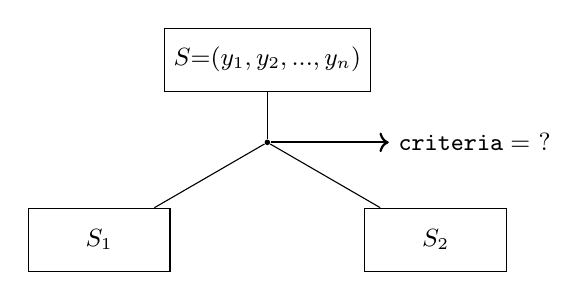
\begin{tikzpicture}[
    node distance=0.8cm,
    box/.style={rectangle, draw, minimum width=1.8cm, minimum height=0.8cm, text centered, font=\small},
    dot/.style={circle, fill=black, minimum size=2pt, inner sep=0pt},
    arrow/.style={->, thick}
]
% Main parent node
\node[box] (parent) {$S$=\\$(y_1, y_2, ..., y_n)$};
% Split point (dot in the middle)
\node[dot, below=0.6cm of parent] (split) {};
% Two child nodes
\node[box, below left=0.8cm and 1.2cm of split] (left) {$S_1$};
\node[box, below right=0.8cm and 1.2cm of split] (right) {$S_2$};
% Connections
\draw (parent) -- (split);
\draw (split) -- (left);
\draw (split) -- (right);
% Loss function arrow and equation
\node[right=1.5cm of split, font=\small] (loss) {$\texttt{criteria} = $ ?};
\draw[arrow] (split) -- (loss);
\end{tikzpicture}

\label{fig:decision_tree_split}
\end{figure}



    \end{column}
\begin{column}{0.6\linewidth}
\vspace{1cm}
$\qquad \qquad$A binary decision tree
\vspace

\resizebox{1\linewidth}{!}{%
        \begin{tikzpicture}[
  level/.style={sibling distance=60mm/#1},
  every node/.style={circle, draw, minimum size=8mm, font=\tiny},
  dots/.style={draw=none, font=\large}
]
\node {Root}
  child {
    node {L1}
    child {
      node {L2}
      child {
        node[dots] {$\vdots$}
      }
      child {
        node[dots] {$\vdots$}
      }
    }
    child {
      node {L2}
      child {
        node[dots] {$\vdots$}
      }
      child {
        node[dots] {$\vdots$}
      }
    }
  }
  child {
    node {R1}
    child {
      node {L2}
      child {
        node[dots] {$\vdots$}
      }
      child {
        node[dots] {$\vdots$}
      }
    }
    child {
      node {L2}
      child {
        node[dots] {$\vdots$}
      }
      child {
        node[dots] {$\vdots$}
      }
    }
  };
\end{tikzpicture}}
    \end{column}

    
\end{columns}


}

\end{frame}






\begin{frame}{}\only<1>{\frametitle{MSE splitting}
\note{Just for a very brief explanation: Let’s consider a node of a decision tree with \( n \) observations and \( m \) covariates. When we  want to split the data, we need a partition rule:

\begin{itemize}
  \item \textbf{First}, we need to decide which covariate, among the \( m \), should be used for the split.
  \item \textbf{Second}, we need to determine a split value, let’s call it \( c \).
\end{itemize}


}
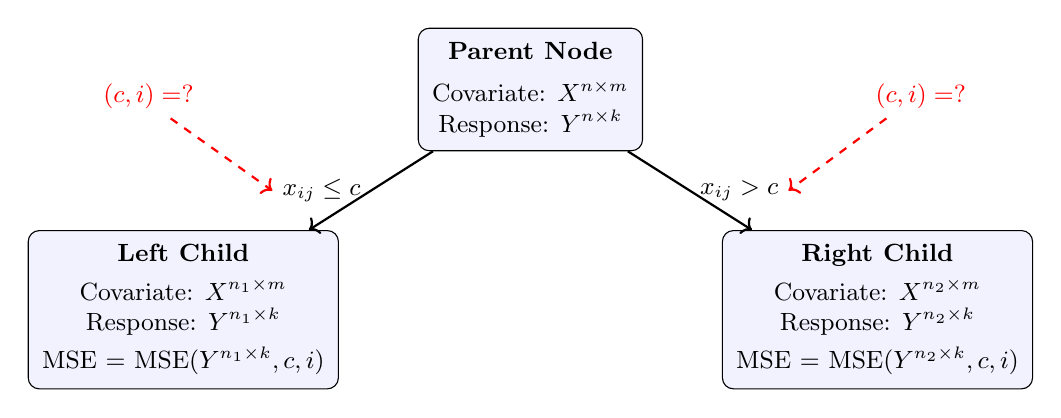
\begin{tikzpicture}[
  node distance=1cm and 1cm,
  every node/.style={font=\small},
  data/.style={rectangle, draw, align=center, fill=blue!5, rounded corners, inner sep=5pt},
  split/.style={->, thick},
  highlight/.style={->, red, thick, dashed}
  ]
  % Parent node
  \node[data] (parent) {
    \textbf{Parent Node} \\[0.15cm]
    Covariate: $X^{n \times m}$ \\ 
    Response: $Y^{n \times k}$
  };
  % Left child
  \node[data, below left=of parent] (left) {
    \textbf{Left Child} \\[0.1cm]
    Covariate: $X^{n_1 \times m}$ \\
    Response: $Y^{n_1 \times k}$ \\[0.1cm]
    MSE = $\text{MSE}(Y^{n_1 \times k},c,i)$
  };
  % Right child
  \node[data, below right=of parent] (right) {
    \textbf{Right Child} \\[0.1cm]
    Covariate: $X^{n_2 \times m}$ \\
    Response: $Y^{n_2 \times k}$ \\[0.1cm]
    MSE = $\text{MSE}(Y^{n_2 \times k},c,i)$
  };
  % Arrows
  \draw[split] (parent) -- node[midway, left] (leftlabel) {$x_{ij} \leq c$} (left);
  \draw[split] (parent) -- node[midway, right] (rightlabel) {$x_{ij} > c$} (right);
  
  % Optimize labels
  \node[red, left] (opt_i) at ([xshift=-1.5cm, yshift=1.2cm]leftlabel) {\textbf{ } $(c,i)=?$};
  \node[red, right] (opt_c) at ([xshift=1.5cm, yshift=1.2cm]rightlabel) {\textbf{} $(c,i)=?$};
  
  % Short highlight arrows from labels to split conditions
  \draw[highlight] (opt_i) -- (leftlabel.west);
  \draw[highlight] (opt_c) -- (rightlabel.east);
\end{tikzpicture}


}
\only<2>{
\note{For example, assume we choose a splitting rule based on covariate 2, and the split value is 3.1.

What we do is very simple. We go to the second column of the table, and for each observation:

if the value is less than 3.1, we assign it to the left node,
if the value is greater than or equal to 3.1, we assign it to the right node.


Now the main question is: how do we choose the best split? or what is the optimal partition rule?



And more importantly, what does “best” actually mean in this context?

This is exactly where the learning criterion comes in, and it defines how the tree grows.}
\frametitle{Split rule}
\begin{columns}[T]

  \column{0.8\textwidth}
 \begin{center}
\renewcommand{\arraystretch}{1.6}
\begin{tabular}{c|c>{\columncolor{purple!20}}cc>{\columncolor{purple!20}}cc|ccc|c}
\textbf{obs} & $x_1$ & \cellcolor{purple!50}$x_2$ & $x_3$ & \cellcolor{purple!20}$x_4$ & $x_5$ & $y_1$ & $y_2$ & $y_3$ & \textbf{child} \\
\hline
\rowcolor{blue!15}
1 & 0.8 & \textbf{1.2} & 3.4 & 0.5 & 2.1 & 0.60 & 0.25 & 0.15 & \textcolor{blue!80!black}{$\leftarrow$ left} \\
\rowcolor{blue!15}
2 & 2.3 & \textbf{2.7} & 1.1 & 4.2 & 0.9 & 0.10 & 0.70 & 0.20 & \textcolor{blue!80!black}{$\leftarrow$ left} \\
\rowcolor{blue!15}
3 & 1.5 & \textbf{3.1} & 2.9 & 1.8 & 3.3 & 0.45 & 0.45 & 0.10 & \textcolor{blue!80!black}{$\leftarrow$ left} \\
\rowcolor{red!15}
4 & 3.9 & \textbf{4.4} & 0.7 & 3.1 & 1.4 & 0.05 & 0.15 & 0.80 & \textcolor{red!80!black}{right $\rightarrow$} \\
\rowcolor{blue!15}
5 & 0.4 & \textbf{2.0} & 4.5 & 2.7 & 5.0 & 0.50 & 0.30 & 0.20 & \textcolor{blue!80!black}{$\leftarrow$ left} \\
\rowcolor{red!15}
6 & 2.1 & \textbf{5.6} & 3.8 & 0.3 & 2.2 & 0.02 & 0.08 & 0.90 & \textcolor{red!80!black}{right $\rightarrow$} \\
\rowcolor{red!15}
7 & 3.3 & \textbf{3.8} & 1.6 & 4.9 & 0.6 & 0.03 & 0.12 & 0.85 & \textcolor{red!80!black}{right $\rightarrow$} \\
\rowcolor{blue!15}
8 & 1.1 & \textbf{1.5} & 2.2 & 1.1 & 4.4 & 0.55 & 0.35 & 0.10 & \textcolor{blue!80!black}{$\leftarrow$ left} \\
\end{tabular}
\end{center}

  \column{0.22\textwidth}
  \vspace{1em}
  \begin{block}{Partition rule}
    Covariate 2: $i=2$ \\ Split value: $c =3.1$\\
    
  \end{block}
  \vspace{0.8em}
  \textcolor{blue!80!black}{\textbf{Left}} \\
  \hspace{0.5em} $x_2 \leq 3.1$ \\[0.2em]
  \hspace{0.5em} obs: 1, 2, 3, 5, 8 \\[0.6em]
  \textcolor{red!80!black}{\textbf{Right}} \\
   \hspace{0.5em} $x_2 > 3.1$ \\
  \hspace{0.5em} obs: 4, 6, 7


\end{columns}
}


\end{frame}




% %--- SLIDE 1: The data ---
% \begin{frame}{Growing a Tree: The Data}
% \begin{columns}[T]

%   \column{0.65\textwidth}
%   \begin{center}
%   \renewcommand{\arraystretch}{1.6}
%   \begin{tabular}{c|ccccc|ccc}
%   \textbf{obs} & $x_1$ & $x_2$ & $x_3$ & $x_4$ & $x_5$ & $y_1$ & $y_2$ & $y_3$ \\
%   \hline
%   1 & 0.8 & 1.2 & 3.4 & 0.5 & 2.1 & 0.60 & 0.25 & 0.15 \\
%   2 & 2.3 & 2.7 & 1.1 & 4.2 & 0.9 & 0.10 & 0.70 & 0.20 \\
%   3 & 1.5 & 3.1 & 2.9 & 1.8 & 3.3 & 0.45 & 0.45 & 0.10 \\
%   4 & 3.9 & 4.4 & 0.7 & 3.1 & 1.4 & 0.05 & 0.15 & 0.80 \\
%   5 & 0.4 & 2.0 & 4.5 & 2.7 & 5.0 & 0.50 & 0.30 & 0.20 \\
%   6 & 2.1 & 5.6 & 3.8 & 0.3 & 2.2 & 0.02 & 0.08 & 0.90 \\
%   7 & 3.3 & 3.8 & 1.6 & 4.9 & 0.6 & 0.03 & 0.12 & 0.85 \\
%   8 & 1.1 & 1.5 & 2.2 & 1.1 & 4.4 & 0.55 & 0.35 & 0.10 \\
%   \end{tabular}
%   \end{center}

%   \column{0.32\textwidth}
%   \vspace{1em}
%   \begin{block}{Setup}
%     Each node holds $n$ observations with $p$ covariates.
%   \end{block}
%   \vspace{0.8em}
%   \textbf{Response} $\mathbf{y}$ is compositional:
%   \[
%     \mathbf{y} = (y_1, y_2, y_3)
%   \]
%   \[
%     y_k \geq 0, \quad \textstyle\sum_k y_k = 1
%   \]
%   \vspace{0.4em}
%   Lives on the simplex $\mathcal{S}^2$.

% \end{columns}
% \end{frame}


% %--- SLIDE 2: Select covariates ---
% \begin{frame}{Step 1 — Select Covariates}
% \begin{columns}[T]

%   \column{0.65\textwidth}
%   \begin{center}
%   \renewcommand{\arraystretch}{1.6}
%   \begin{tabular}{c|c>{\columncolor{purple!20}}cc>{\columncolor{purple!20}}cc|ccc}
%   \textbf{obs} & $x_1$ & \cellcolor{purple!50}$x_2$ & $x_3$ & \cellcolor{purple!50}$x_4$ & $x_5$ & $y_1$ & $y_2$ & $y_3$ \\
%   \hline
%   1 & 0.8 & 1.2 & 3.4 & 0.5 & 2.1 & 0.60 & 0.25 & 0.15 \\
%   2 & 2.3 & 2.7 & 1.1 & 4.2 & 0.9 & 0.10 & 0.70 & 0.20 \\
%   3 & 1.5 & 3.1 & 2.9 & 1.8 & 3.3 & 0.45 & 0.45 & 0.10 \\
%   4 & 3.9 & 4.4 & 0.7 & 3.1 & 1.4 & 0.05 & 0.15 & 0.80 \\
%   5 & 0.4 & 2.0 & 4.5 & 2.7 & 5.0 & 0.50 & 0.30 & 0.20 \\
%   6 & 2.1 & 5.6 & 3.8 & 0.3 & 2.2 & 0.02 & 0.08 & 0.90 \\
%   7 & 3.3 & 3.8 & 1.6 & 4.9 & 0.6 & 0.03 & 0.12 & 0.85 \\
%   8 & 1.1 & 1.5 & 2.2 & 1.1 & 4.4 & 0.55 & 0.35 & 0.10 \\
%   \end{tabular}
%   \end{center}

%   \column{0.32\textwidth}
%   \vspace{1em}
%   \begin{block}{Random subspace}
%     At each node, draw $m \leq p$ covariates at random.
%   \end{block}
%   \vspace{0.8em}
%   \textcolor{purple!80!black}{\textbf{Selected:}} $x_2,\, x_4$
%   \vspace{0.6em}

%   \begin{itemize}[label={\ding{226}}]
%     \item Reduces correlation between trees
%     \item Only \textcolor{purple!80!black}{highlighted columns} are split candidates
%     \item Other columns are ignored at this node
%   \end{itemize}

% \end{columns}
% \end{frame}


% %--- SLIDE 3: Find the best split ---
% \begin{frame}{Step 2 — Find the Best Split}
% \begin{columns}[T]

%   \column{0.72\textwidth}
%   \begin{center}
%   \renewcommand{\arraystretch}{1.6}
%   \begin{tabular}{c|c>{\columncolor{purple!20}}cc>{\columncolor{purple!20}}cc|ccc|c}
%   \textbf{obs} & $x_1$ & \cellcolor{purple!50}$x_2$ & $x_3$ & \cellcolor{purple!20}$x_4$ & $x_5$ & $y_1$ & $y_2$ & $y_3$ & \\
%   \hline
%   \rowcolor{leftblue}
%   1 & 0.8 & \textbf{1.2} & 3.4 & 0.5 & 2.1 & 0.60 & 0.25 & 0.15 & \textcolor{blue!80!black}{$\leftarrow$ left} \\
%   \rowcolor{leftblue}
%   2 & 2.3 & \textbf{2.7} & 1.1 & 4.2 & 0.9 & 0.10 & 0.70 & 0.20 & \textcolor{blue!80!black}{$\leftarrow$ left} \\
%   \rowcolor{leftblue}
%   3 & 1.5 & \textbf{3.1} & 2.9 & 1.8 & 3.3 & 0.45 & 0.45 & 0.10 & \textcolor{blue!80!black}{$\leftarrow$ left} \\
%   \rowcolor{rightred}
%   4 & 3.9 & \textbf{4.4} & 0.7 & 3.1 & 1.4 & 0.05 & 0.15 & 0.80 & \textcolor{red!80!black}{right $\rightarrow$} \\
%   \rowcolor{leftblue}
%   5 & 0.4 & \textbf{2.0} & 4.5 & 2.7 & 5.0 & 0.50 & 0.30 & 0.20 & \textcolor{blue!80!black}{$\leftarrow$ left} \\
%   \rowcolor{rightred}
%   6 & 2.1 & \textbf{5.6} & 3.8 & 0.3 & 2.2 & 0.02 & 0.08 & 0.90 & \textcolor{red!80!black}{right $\rightarrow$} \\
%   \rowcolor{rightred}
%   7 & 3.3 & \textbf{3.8} & 1.6 & 4.9 & 0.6 & 0.03 & 0.12 & 0.85 & \textcolor{red!80!black}{right $\rightarrow$} \\
%   \rowcolor{leftblue}
%   8 & 1.1 & \textbf{1.5} & 2.2 & 1.1 & 4.4 & 0.55 & 0.35 & 0.10 & \textcolor{blue!80!black}{$\leftarrow$ left} \\
%   \end{tabular}
%   \end{center}

%   \column{0.25\textwidth}
%   \vspace{1em}
%   \begin{block}{Partition rule}
%     \textcolor{purple!80!black}{Best:} $x_2 \leq 3.5$
%   \end{block}
%   \vspace{0.8em}
%   \textcolor{blue!80!black}{\textbf{Left}} \hfill $x_2 \leq 3.5$\\[0.2em]
%   \hspace{0.5em} obs: 1,2,3,5,8 \\[0.6em]
%   \textcolor{red!80!black}{\textbf{Right}} \hfill $x_2 > 3.5$ \\[0.2em]
%   \hspace{0.5em} obs: 4,6,7
%   \vspace{0.6em}



% \end{columns}
% \end{frame}





\begin{frame}{}\only<1>{\frametitle{MSE splitting}
\note{Just for a very brief explanation: Let’s consider a node of a decision tree with \( n \) observations and \( m \) covariates. When we  want to split the data, we face two key decisions:

\begin{itemize}
  \item \textbf{First}, we need to decide which covariate, among the \( m \), should be used for the split.
  \item \textbf{Second}, we need to determine a split value, let’s call it \( c \).
\end{itemize}


So, the problem is to find the optimal pair \( (i, c) \).  For regression trees, the usual splitting criterion is the mean squared error (MSE). 

The mean squared error (MSE) does not account for the simplex constraint.
}
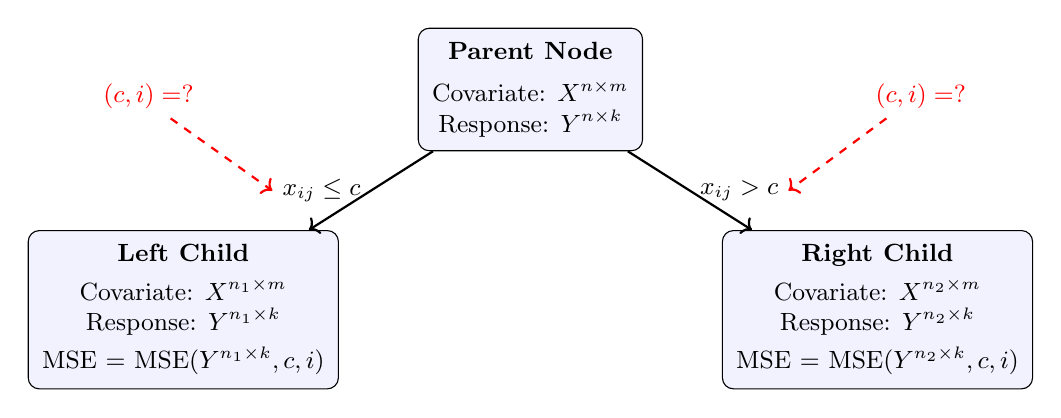
\begin{tikzpicture}[
  node distance=1cm and 1cm,
  every node/.style={font=\small},
  data/.style={rectangle, draw, align=center, fill=blue!5, rounded corners, inner sep=5pt},
  split/.style={->, thick},
  highlight/.style={->, red, thick, dashed}
  ]
  % Parent node
  \node[data] (parent) {
    \textbf{Parent Node} \\[0.15cm]
    Covariate: $X^{n \times m}$ \\ 
    Response: $Y^{n \times k}$
  };
  % Left child
  \node[data, below left=of parent] (left) {
    \textbf{Left Child} \\[0.1cm]
    Covariate: $X^{n_1 \times m}$ \\
    Response: $Y^{n_1 \times k}$ \\[0.1cm]
    MSE = $\text{MSE}(Y^{n_1 \times k},c,i)$
  };
  % Right child
  \node[data, below right=of parent] (right) {
    \textbf{Right Child} \\[0.1cm]
    Covariate: $X^{n_2 \times m}$ \\
    Response: $Y^{n_2 \times k}$ \\[0.1cm]
    MSE = $\text{MSE}(Y^{n_2 \times k},c,i)$
  };
  % Arrows
  \draw[split] (parent) -- node[midway, left] (leftlabel) {$x_{ij} \leq c$} (left);
  \draw[split] (parent) -- node[midway, right] (rightlabel) {$x_{ij} > c$} (right);
  
  % Optimize labels
  \node[red, left] (opt_i) at ([xshift=-1.5cm, yshift=1.2cm]leftlabel) {\textbf{ } $(c,i)=?$};
  \node[red, right] (opt_c) at ([xshift=1.5cm, yshift=1.2cm]rightlabel) {\textbf{} $(c,i)=?$};
  
  % Short highlight arrows from labels to split conditions
  \draw[highlight] (opt_i) -- (leftlabel.west);
  \draw[highlight] (opt_c) -- (rightlabel.east);
\end{tikzpicture}

\begin{equation*}
    
(c^*, i^*) 
&=& \operatorname{argmin}_{i,c} \left( \text{MSE}(Y^{n_1 \times k},c,i) + \text{MSE}(Y^{n_2 \times k},c,i) \right)
\\
&=& \arg\min_{c,j} 
\left\{\frac{n_1(c,j)}{n}
\sum_{m=1}^k \sum_{i=1}^{n_1(c,j)} (y_{im}-\bar{y}_{m}^{n_1(c,j)})^2
+
\frac{n_2(c,j)}{n}
\sum_{m=1}^k \sum_{i=1}^{n_2(c,j)} (y_{im}-\bar{y}_{m}^{n_2(c,j)})^2
\right\}.
\end{equation*}

}



\only<2>{ \frametitle{MSE splitting}
\note{ But using mse has a problem, which is that in simplex space, the component variance usually depends on E. for example, if the outcome variable follows a Dirichlet distribution, obviously the variance depends on the mean parameter \(\mu\). This is a violation of the homoscedasticity assumption.

One possible idea is to use maximum likelihood instead of distance measures. In this approach, each node is split into two child nodes in a way that gives the best overall likelihood.

To solve this, we use the total \textbf{log-likelihood} under the Dirichlet distribution.


}
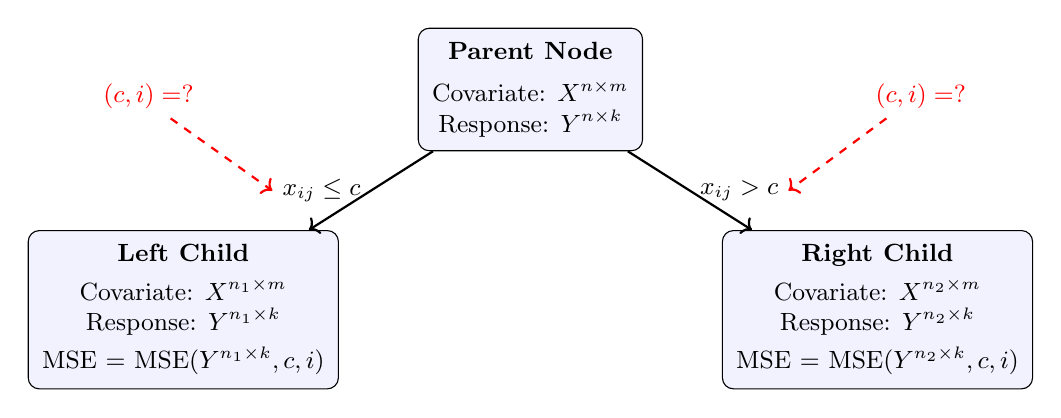
\begin{tikzpicture}[
  node distance=1cm and 1cm,
  every node/.style={font=\small},
  data/.style={rectangle, draw, align=center, fill=blue!5, rounded corners, inner sep=5pt},
  split/.style={->, thick},
  highlight/.style={->, red, thick, dashed}
  ]
  % Parent node
  \node[data] (parent) {
    \textbf{Parent Node} \\[0.15cm]
    Covariate: $X^{n \times m}$ \\ 
    Response: $Y^{n \times k}$
  };
  % Left child
  \node[data, below left=of parent] (left) {
    \textbf{Left Child} \\[0.1cm]
    Covariate: $X^{n_1 \times m}$ \\
    Response: $Y^{n_1 \times k}$ \\[0.1cm]
    MSE = $\text{MSE}(Y^{n_1 \times k},c,i)$
  };
  % Right child
  \node[data, below right=of parent] (right) {
    \textbf{Right Child} \\[0.1cm]
    Covariate: $X^{n_2 \times m}$ \\
    Response: $Y^{n_2 \times k}$ \\[0.1cm]
    MSE = $\text{MSE}(Y^{n_2 \times k},c,i)$
  };
  % Arrows
  \draw[split] (parent) -- node[midway, left] (leftlabel) {$x_{ij} \leq c$} (left);
  \draw[split] (parent) -- node[midway, right] (rightlabel) {$x_{ij} > c$} (right);
  
  % Optimize labels
  \node[red, left] (opt_i) at ([xshift=-1.5cm, yshift=1.2cm]leftlabel) {\textbf{ } $(c,i)=?$};
  \node[red, right] (opt_c) at ([xshift=1.5cm, yshift=1.2cm]rightlabel) {\textbf{} $(c,i)=?$};
  
  % Short highlight arrows from labels to split conditions
  \draw[highlight] (opt_i) -- (leftlabel.west);
  \draw[highlight] (opt_c) -- (rightlabel.east);
\end{tikzpicture}
\begin{itemize}
    \item 
MSE does not account for the simplex constraint.

\item 
\[V(X_i)=\frac{E(X_i)\left(1-E(X_i)\right)}{\alpha_0+1}\]
\end{itemize}

}

\end{frame}







\begin{frame}
\only<1>{
\frametitle{Dirichlet distribution}
\note{The only familiar class of distributions on simplex space is dirichlet distribution. This model operates directly on the simplex without requiring the data to be transformed into another space.

Other distributions have also been developed for compositional data, but most of them are based on transformations. In this work, we use the Dirichlet distribution.
}


\vspace{1em}

\begin{center}
\colorbox{green!10}{\parbox{0.95\textwidth}{
\begin{center}
\resizebox{\linewidth}{!}{%
\[
    f_{\mathbf{Z}}((z_1,\ldots,z_k); \boldsymbol{\alpha}) = \frac{\Gamma( \alpha_0)}{\prod_{i=1}^k \Gamma(\alpha_i)} \prod_{i=1}^k z_i^{\alpha_i - 1},
\quad  z_i \in [0, 1], \quad \sum_{i=1}^k z_i = 1,
\]
}
\end{center}
}}
\end{center}

\vspace{1.5em}

\begin{itemize}[itemsep=0.8em]


\item[\textcolor{blue}{\large$\blacktriangleright$}] The sum-constant requirement of the simplex is satisfied under the Dirichlet distribution.

\item[\textcolor{blue}{\large$\blacktriangleright$}] \textbf{Extensions available:} Zero-inflated Dirichlet and Kummer–Dirichlet
\end{itemize}
}

\end{frame}


\begin{frame}
\only<1>{\frametitle{Dirichlet log-likelihood splitting}
\note{



\vspace{1em}
We approach this optimization by maximizing the total log-likelihood. Specifically, for each candidate split \( (i, c) \), we compute the log-likelihoods of the two resulting sub-nodes, sum them, and identify the pair \( (i, c) \) that yields the highest total log-likelihood.

\vspace{1em}
The remaining steps follow the standard decision tree procedure.

\vspace{1em}
With this modification, we obtain a random forest—referred to as the \textbf{Dirichlet Random Forest}—which can be applied directly to compositional data, without requiring transformation.


}
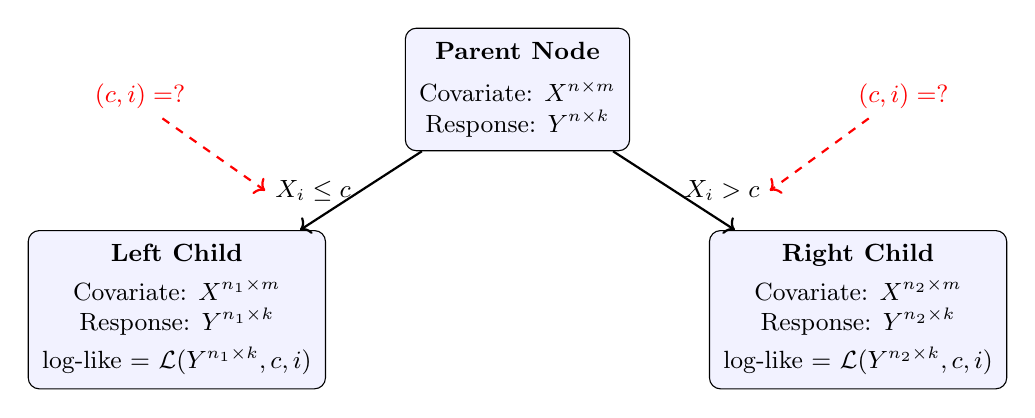
\begin{tikzpicture}[
  node distance=1cm and 1cm,
  every node/.style={font=\small},
  data/.style={rectangle, draw, align=center, fill=blue!5, rounded corners, inner sep=5pt},
  split/.style={->, thick},
  highlight/.style={->, red, thick, dashed}
  ]
  % Parent node
  \node[data] (parent) {
    \textbf{Parent Node} \\[0.15cm]
    Covariate: $X^{n \times m}$ \\ 
    Response: $Y^{n \times k}$
  };
  % Left child
  \node[data, below left=of parent] (left) {
    \textbf{Left Child} \\[0.1cm]
    Covariate: $X^{n_1 \times m}$ \\
    Response: $Y^{n_1 \times k}$ \\[0.1cm]
     log-like = $\mathcal{L}(Y^{n_1 \times k},c,i)$
  };
  % Right child
  \node[data, below right=of parent] (right) {
    \textbf{Right Child} \\[0.1cm]
    Covariate: $X^{n_2 \times m}$ \\
    Response: $Y^{n_2 \times k}$ \\[0.1cm]
     log-like = $\mathcal{L}(Y^{n_2 \times k},c,i)$
  };
  % Arrows
  \draw[split] (parent) -- node[midway, left] (leftlabel) {$X_{i} \leq c$} (left);
  \draw[split] (parent) -- node[midway, right] (rightlabel) {$X_{i} > c$} (right);
  
  % Optimize labels
  \node[red, left] (opt_i) at ([xshift=-1.5cm, yshift=1.2cm]leftlabel) {\textbf{ } $(c,i)=?$};
  \node[red, right] (opt_c) at ([xshift=1.5cm, yshift=1.2cm]rightlabel) {\textbf{} $(c,i)=?$};
  
  % Short highlight arrows from labels to split conditions
  \draw[highlight] (opt_i) -- (leftlabel.west);
  \draw[highlight] (opt_c) -- (rightlabel.east);
\end{tikzpicture}
\[
(c^*, i^*) = \operatorname{argmax}_{i,c} \left( \max_{\boldsymbol{\alpha}} \mathcal{L}(Y^{n_1 \times k},c,i) + \max_{\boldsymbol{\alpha}} \mathcal{L}(Y^{n_2 \times k},c,i) \right)
\]
}
\end{frame}

\begin{frame}{Prediction based on DirichletRF}
\note{
    By considering the Dirichlet distribution, we eventually obtain several terminal nodes, each containing a set of observations. For a new observation, we traverse the decision tree to identify the corresponding terminal node. 

    default: 
    
    In a regression decision tree, we then have two options for prediction: either use the mean of the observations in that node, or use the estimated parameters of the Dirichlet distribution as the prediction.

    In a random forest, we repeat this process for many trees and finally take the mean of the predictions from all the trees.

    another idea:
    
Then, in that terminal node, we have a set of observations.

In a random forest, we repeat this process for many trees, and in the end we obtain several terminal nodes, each one associated with a different tree. We use these observations to construct an empirical probability function.

    }
    
\begin{columns}[T]

% Left column - Graph
\begin{column}{0.45\textwidth}
\centering
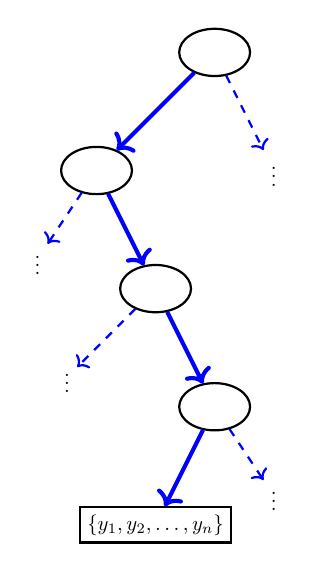
\begin{tikzpicture}[
    node/.style={ellipse, draw, minimum width=1.2cm, minimum height=0.8cm, thick},
    leaf/.style={rectangle, draw, minimum width=1.8cm, minimum height=0.6cm, thick},
    arrow/.style={->, thick, blue},
    scale=0.75,
    every node/.style={transform shape}
]

% Root node
\node[node] (root) at (0,0) {};

% Level 1
\node[node] (n1) at (-2,-2) {};
\node (dots1) at (1,-2) {\vdots};

% Level 2
\node (dots2) at (-3,-3.5) {\vdots};
\node[node] (n2) at (-1,-4) {};

% Level 3
\node (dots3) at (-2.5,-5.5) {\vdots};
\node[node] (n3) at (0,-6) {};

% Level 4
\node (dots4) at (1,-7.5) {\vdots};
\node[leaf] (leaf) at (-1,-8) {$\{y_1, y_2, \ldots, y_n\}$};

% Arrows - traversal path highlighted
\draw[arrow, line width=1.5pt] (root) -- (n1);
\draw[arrow, dashed] (root) -- (dots1);
\draw[arrow, dashed] (n1) -- (dots2);
\draw[arrow, line width=1.5pt] (n1) -- (n2);
\draw[arrow, dashed] (n2) -- (dots3);
\draw[arrow, line width=1.5pt] (n2) -- (n3);
\draw[arrow, line width=1.5pt] (n3) -- (leaf);
\draw[arrow, dashed] (n3) -- (dots4);

\end{tikzpicture}
\end{column}

% Right column - Explanation
\begin{column}{0.52\textwidth}
\small

\textbf{Process:}
\begin{itemize}[label=\arabic*.]
    \item Start at root node
    \item Traverse tree based on decision rules
    \item Reach terminal node with observations
\end{itemize}

\vspace{0.4cm}

\textbf{Default Approach:}
\begin{itemize}
    \item Mean: $\hat{y} = \frac{1}{n}\sum_{i=1}^{n} y_i$
    \item Expectation: $\text{E}(Y_i) = \frac{\hat{\alpha}_i}{\sum_{j+1}^k\hat{\alpha}_i}$
    \item Random Forest: average across trees
\end{itemize}

\vspace{0.4cm}

\textbf{Distributional Approach:}
\begin{itemize}
    \item Collect terminal nodes from all trees
    \item Construct empirical probability function
\end{itemize}

\end{column}

\end{columns}

\end{frame}












%\begin{frame}{Comparison Results}
      \centering
      \vfill
      \textbf{\Large Comparison Results}
      \vfill
\end{frame}

\begin{frame}{Performance Evaluation and Transformations}

To evaluate DirichletRF's performance, we compare it with two alternative approaches:
\begin{itemize}
    \item[1)] \textbf{ILR-RF:} A Random Forest model based on log-ratio transformations. 
    The compositional data are first transformed into the ILR
    space. Then, a standard Random Forest is applied to the transformed data, and 
    finally, the predictions are mapped back to the simplex for interpretation.

    \item[2)] \textbf{Dirichlet Regression:} A parametric approach that, 
    works directly on the simplex without requiring any transformation.
\end{itemize}

\end{frame}




\begin{frame}{Evaluation Metrics}
\note{
To compare these models, we used  the Aitchison Distance and the Root Mean Square Error, or RMSE.

The Aitchison Distance is the usual Euclidean distance between them.

On the other hand, RMSE is a widely used and well-known metric. Unlike the Aitchison Distance, it does not take into account the geometric structure of the simplex
}
To compare these models, we used  the Aitchison Distance and the Root Mean Square Error, or RMSE.
\vspace{0.2cm}
\textbf{1. Aitchison Distance:}
\[
AC = \frac{1}{n} \sum_{i=1}^n \sqrt{\sum_{j=1}^k \left(\log\frac{Y_{ij}}{g(\mathbf{Y}_i)} - \log\frac{\hat{Y}_{ij}}{g(\hat{\mathbf{Y}}_i)}\right)^2},
\]
\[
\text{where} \quad g(\mathbf{Y}_i) = \left(\prod_{j=1}^k Y_{ij}\right)^{1/k}
\]
\textit{Measures compositional dissimilarity using log-ratio geometry.}

\vspace{0.3cm}
\textbf{2. Root Mean Square Error (RMSE):}
$
\text{RMSE}_k =  \sqrt{\frac{1}{n} \sum_{i=1}^n (Y_{ij} - \hat{Y}_{ij})^2}
$

\vspace{0.3cm}
\textbf{Interpretation:} Lower values for both metrics indicate better predictive accuracy.
\end{frame}








\begin{frame}{}

    \only<1>{
    \note{We generated two datasets — one simple and one more complex. Here, we used three covariates and a three-dimensional compositional response. The response data was generated from a Dirichlet distribution with a simple, linear relationship to the covariates.}
    \textbf{Simple structure simulations}: We use a simple dataset with $3$ Covariate variables, $X_1,X_1, X_{3}$ and with a $3$-dimensional response, $(Y_1,\,Y_2,\,Y_3)$ such that $Y_1+Y_2+Y_3 = 1$. The response is assumed to follow a Dirichlet distribution with the following parameters:
\[
\alpha_1 = 1 + 2 X_1,\quad \alpha_2 =1 + 0.5 X_2,\quad \alpha_3 = 1 + X_3.
\]
\[
(Y_1,\,Y_2,\,Y_3)\sim Dirichlet(\alpha_1,\alpha_2,\alpha_3)
\]
    }
    \only<2>{
    \note{In this table, you can see the results for the this dataset across different sample sizes.
The first and second columns show the performance of each model based on the both metrics measured on the test set.
The last column shows the difference between the Aitchison Distance on the test and train datasets, which gives us insight into overfitting.

Dirichlet Regression performed better than the other models. This result makes sense, because the data was generated using a Dirichlet distribution with a linear structure.

But, Dirichlet Random Forest does not perform well in this case — in fact, it gives the worst performance in terms of Aitchison Distance and RMSE.

It just performs better than CLR-RF and ILR-RF when it comes to overfitting.

So, we can say that in this example, the main advantage of Dirichlet Random Forest compared to the other RF models is that it is more robust against overfitting.}
    
\begin{table}[htbp]
\centering
\small 
\begin{tabular}{|l|l|c|c|c|c|}
\hline
$N$ & Model & Aitchison Distance  & RMSE & Train-Test \\
\hline

{200} 
    & CLR-RF & 1.299 (0.141) & 0.703 (0.039) & 0.684 \\
    & ILR-RF & 1.303 (0.143) & 0.700 (0.040)& 0.686 \\
    & \textcolor{blue}{Dirichlet Regression} & \textcolor{blue}{\textbf{1.233} (0.139)} & \textcolor{blue}{\textbf{0.745} (0.033)}  & \textcolor{blue}{\textbf{0.030}} \\
    & \texttt{Dirichlet-RF} & 1.451 (0.153) & 0.620 (0.052)  & 0.600 \\
\hline
{500}
    & CLR-RF & 1.282 (0.077) & 0.716 (0.019)  & 0.684 \\
    & ILR-RF & 1.284 (0.077) & 0.716 (0.020)& 0.685 \\
    & \textcolor{blue}{Dirichlet Regression} & \textcolor{blue}{\textbf{1.234} (0.078)} & \textcolor{blue}{\textbf{0.752} (0.016)}  & \textcolor{blue}{\textbf{0.035}} \\
    & \texttt{Dirichlet-RF} & 1.450 (0.077) & 0.627 (0.031) & 0.616 \\
\hline
{2000}
    & CLR-RF & 1.249 (0.032) & 0.726 (0.010) & 0.652 \\
    & ILR-RF & 1.252 (0.032) & 0.725 (0.010)  & 0.654 \\
    & \textcolor{blue}{Dirichlet Regression} & \textcolor{blue}{\textbf{1.209} (0.032)} & \textcolor{blue}{\textbf{0.757} (0.008)}  & \textcolor{blue}{\textbf{0.006}} \\
    & \texttt{Dirichlet-RF} & 1.431 (0.041) & 0.635 (0.016) & 0.596 \\
\hline
\end{tabular}
\caption{ Values represent the means and (standard deviations) of the metrics for test datasets. Train-Test Diff represents the absolute difference between train and test Aitchison Distance, indicating model generalisation capability. }
\label{tab:performance-comparison1}
\end{table}}

    \only<3>{
    	    
    \note{
We compared these models on various datasets—both simulated and real-world. The performance comparison showed competitive results among the random forest-based models. Sometimes the Dirichlet Random Forest performed best, sometimes not—but it consistently delivered satisfactory outcomes.
One situation where it outperformed the others was when the structure of the dataset was complex. For example,
  consider three-dimensional compositional responses and with 10 covariates — only 3 of them are informative, and the other 7 have no relationship with the response. 
As you can see, the responses are generated from a normal distribution, and the relationship with the three informative covariates is nonlinear — we used functions like sin(x), exp(x), quantile, and other nonlinear forms.


    }
    Complex structure synthetic simulations: The dataset consisted of 10 predictor variables \((X_1, \ldots, X_{10})\), with only the first three variables \((X_1, X_2, X_3)\) being truly informative for predicting the compositional response. The three-component compositional response vector $\mathbf{Y} = (Y_1,Y_2,Y_3)$ was constructed through complex non-linear transformations of the informative Covariates. }
    \end{frame}
\begin{frame}
    \only<1>{

\begin{columns}
\begin{column}{0.5\linewidth}

% where \( \mathcal{N}(\mu_i, 0.5^2) \) represents a normally distributed random variable with mean \( \mu_i \) and standard deviation \( 0.5 \), and \( \epsilon \) is a small positive constant ensuring non-negativity.  
% The compositional response variables \( Y_1, Y_2, Y_3 \) are then obtained via the normalisation:
We generate the variables \( Z_1, Z_2, Z_3 \) as follows:  
\[
Z_i = \max(\epsilon, \mathcal{N}(\mu_i, 0.5)), \quad 
\]
\[
Y_i = \frac{Z_i}{Z_1 + Z_2 + Z_3}, \quad  i = 1,2,3.
\]
% This transformation ensures that \( (Y_1, Y_2, Y_3) \) lies within the unit simplex, preserving the compositional structure of the data.
\end{column}
		\begin{column}{0.5\linewidth}

\begin{align*}
\mu_{1j} &= g(2(1 + \sin(x_{1j}))+x_{2j}^3) \\
\mu_{2j} &= g(1 + 2.5\exp(x_{3j})+x_{1j}^2) \\
\mu_{3j} &= g(1 + (1+x_{2j})^2+x_{3j}^4)
\end{align*}

\end{column}

\end{columns}

Where
\[
g(x_{ij}) =
\begin{cases} 
    2, & x_{ij} < \text{Quantile}(x_i, 0.3) \\
    3, & \text{Quantile}(x_i, 0.3) \leq x_{ij} <\text{Quantile}(x_i, 0.6) \\
    4, & \text{Quantile}(x, 0.6) \leq x_{ij} \leq \text{Quantile}(x_i, 0.8) \\
    1, & x_i > \text{Quantile}(x_i, 0.8)
\end{cases}
\]

}
\end{frame}
\begin{frame}
\only<1>{
\note{In this complex scenario, the results are reversed. Our Dirichlet-RF is now the best model, and Dirichlet Regression is the worst.

In terms of overfitting, Dirichlet Regression still performs the best. But this is expected — we don’t usually expect a random forest model to outperform a parametric model with a simple structure when it comes to overfitting.
However, Dirichlet-RF still performs better than the other two random forest models. Overfitting is a common issue in decision tree-based models, but based on our experience, Dirichlet-RF shows better generalization and less overfitting.
}
\begin{table}[htbp]
\centering
\small 
\begin{tabular}{|l|l|c|c|c|c|}
\hline
N & Model & Aitchison Distance & RMSE & Train-Test \\

\hline
{200} 
    & CLR-RF & 0.671 (0.152) & 0.898 (0.018) & 0.366 \\
    & ILR-RF & 0.670 (0.151) & 0.899 (0.018) & 0.364 \\
    & Dirichlet Regression & 0.826 (0.155) & 0.844 (0.026)  & 0.068 \\
    & \textcolor{blue}{{Dirichlet-RF}} & \textcolor{blue}{\textbf{0.659} (0.152)} & \textcolor{blue}{\textbf{0.903} (0.017)}  & 0.221 \\
\hline
{500} 
    & CLR-RF & 0.617 (0.072) & 0.912 (0.011) &   0.334 \\
    & ILR-RF & 0.618 (0.072) & 0.911 (0.012) &  0.334 \\
    & Dirichlet Regression & 0.790 (0.075) & 0.855 (0.012)  & 0.029 \\
    & \textcolor{blue}{{Dirichlet-RF}} & \textcolor{blue}{\textbf{0.606} (0.068)} & \textcolor{blue}{\textbf{0.917} (0.010)}  & 0.201 \\
\hline
{2000} 
    & CLR-RF & 0.557 (0.045) & 0.931 (0.006) & 0.302 \\
    & ILR-RF & 0.557 (0.044) & 0.931 (0.006)& 0.301 \\
    & Dirichlet Regression & 0.785 (0.044) & 0.858 (0.006)  & 0.016\\
    &\textcolor{blue}{ {Dirichlet-RF}} & \textcolor{blue}{\textbf{0.544} (0.044)} & \textcolor{blue}{\textbf{0.936} (0.004) }& 0.178 \\
\hline
\end{tabular}
\caption{ Train-Test Diff represents the absolute difference between train and test Aitchison Distance.}
\label{tab:performance-comparison}
\end{table}
}
\only<2>{
\note{In this complex scenario, the results are reversed. Our Dirichlet-RF is now the best model, and Dirichlet Regression is the worst.

In terms of overfitting, Dirichlet Regression still performs the best. But this is expected — we don’t usually expect a random forest model to outperform a parametric model with a simple structure when it comes to overfitting.
However, Dirichlet-RF still performs better than the other two random forest models. Overfitting is a common issue in decision tree-based models, but based on our experience, Dirichlet-RF shows better generalization and less overfitting.
}
\begin{table}[htbp]
\centering
\small 
\begin{tabular}{|l|l|c|c|c|c|}
\hline
N & Model & Aitchison Distance & RMSE & Train-Test \\

\hline
{200} 
    & CLR-RF & 0.671 (0.152) & 0.898 (0.018) & 0.366 \\
    & ILR-RF & 0.670 (0.151) & 0.899 (0.018) & 0.364 \\
    & Dirichlet Regression & 0.826 (0.155) & 0.844 (0.026)  & \textcolor{blue}{\textbf{0.068}} \\
    & \textcolor{blue}{{Dirichlet-RF}} & 0.659 (0.152) & 0.903 (0.017)  & 0.221 \\
\hline
{500} 
    & CLR-RF & 0.617 (0.072) & 0.912 (0.011) &   0.334 \\
    & ILR-RF & 0.618 (0.072) & 0.911 (0.012) &  0.334 \\
    & Dirichlet Regression & 0.790 (0.075) & 0.855 (0.012)  & \textcolor{blue}{\textbf{0.029}} \\
    & \textcolor{blue}{{Dirichlet-RF}} & 0.606 (0.068) & 0.917 (0.010)  & 0.201 \\
\hline
{2000} 
    & CLR-RF & 0.557 (0.045) & 0.931 (0.006) & 0.302 \\
    & ILR-RF & 0.557 (0.044) & 0.931 (0.006)& 0.301 \\
    & Dirichlet Regression & 0.785 (0.044) & 0.858 (0.006)  & \textcolor{blue}{\textbf{0.016} }\\
    &\textcolor{blue}{ {Dirichlet-RF}} & 0.544 (0.044) & 0.936 (0.004) & 0.178 \\
\hline
\end{tabular}
\caption{ Train-Test Diff represents the absolute difference between train and test Aitchison Distance.}
\label{tab:performance-comparison}
\end{table}
}

\only<3>{
\note{In this complex scenario, the results are reversed. Our Dirichlet-RF is now the best model, and Dirichlet Regression is the worst.

In terms of overfitting, Dirichlet Regression still performs the best. But this is expected — we don’t usually expect a random forest model to outperform a parametric model with a simple structure when it comes to overfitting.
However, Dirichlet-RF still performs better than the other two random forest models. Overfitting is a common issue in decision tree-based models, but based on our experience, Dirichlet-RF shows better generalization and less overfitting.
}
\begin{table}[htbp]
\centering
\small 
\begin{tabular}{|l|l|c|c|c|c|}
\hline
N & Model & Aitchison Distance & RMSE & Train-Test \\

\hline
{200} 
    & CLR-RF & 0.671 (0.152) & 0.898 (0.018) & 0.366 \\
    & ILR-RF & 0.670 (0.151) & 0.899 (0.018) & 0.364 \\
    & Dirichlet Regression & 0.826 (0.155) & 0.844 (0.026)  & 0.068 \\
    & \textcolor{blue}{{Dirichlet-RF}} & 0.659 (0.152) & 0.903 (0.017)  & \textcolor{blue}{ \textbf{0.221}} \\
\hline
{500} 
    & CLR-RF & 0.617 (0.072) & 0.912 (0.011) &   0.334 \\
    & ILR-RF & 0.618 (0.072) & 0.911 (0.012) &  0.334 \\
    & Dirichlet Regression & 0.790 (0.075) & 0.855 (0.012)  & 0.029 \\
    & \textcolor{blue}{{Dirichlet-RF}} & 0.606 (0.068) & 0.917 (0.010)  & \textcolor{blue}{ \textbf{0.201}} \\
\hline
{2000} 
    & CLR-RF & 0.557 (0.045) & 0.931 (0.006) & 0.302 \\
    & ILR-RF & 0.557 (0.044) & 0.931 (0.006)& 0.301 \\
    & Dirichlet Regression & 0.785 (0.044) & 0.858 (0.006)  & 0.016\\
    &\textcolor{blue}{ {Dirichlet-RF}} & 0.544 (0.044) & 0.936 (0.004) & \textcolor{blue}{ \textbf{0.178}} \\
\hline
\end{tabular}
\caption{ Train-Test Diff represents the absolute difference between train and test Aitchison Distance.}
\label{tab:performance-comparison}
\end{table}
}
\end{frame}

\begin{frame}{Learning Curve}
\only<1>{


\begin{figure}
    \centering
    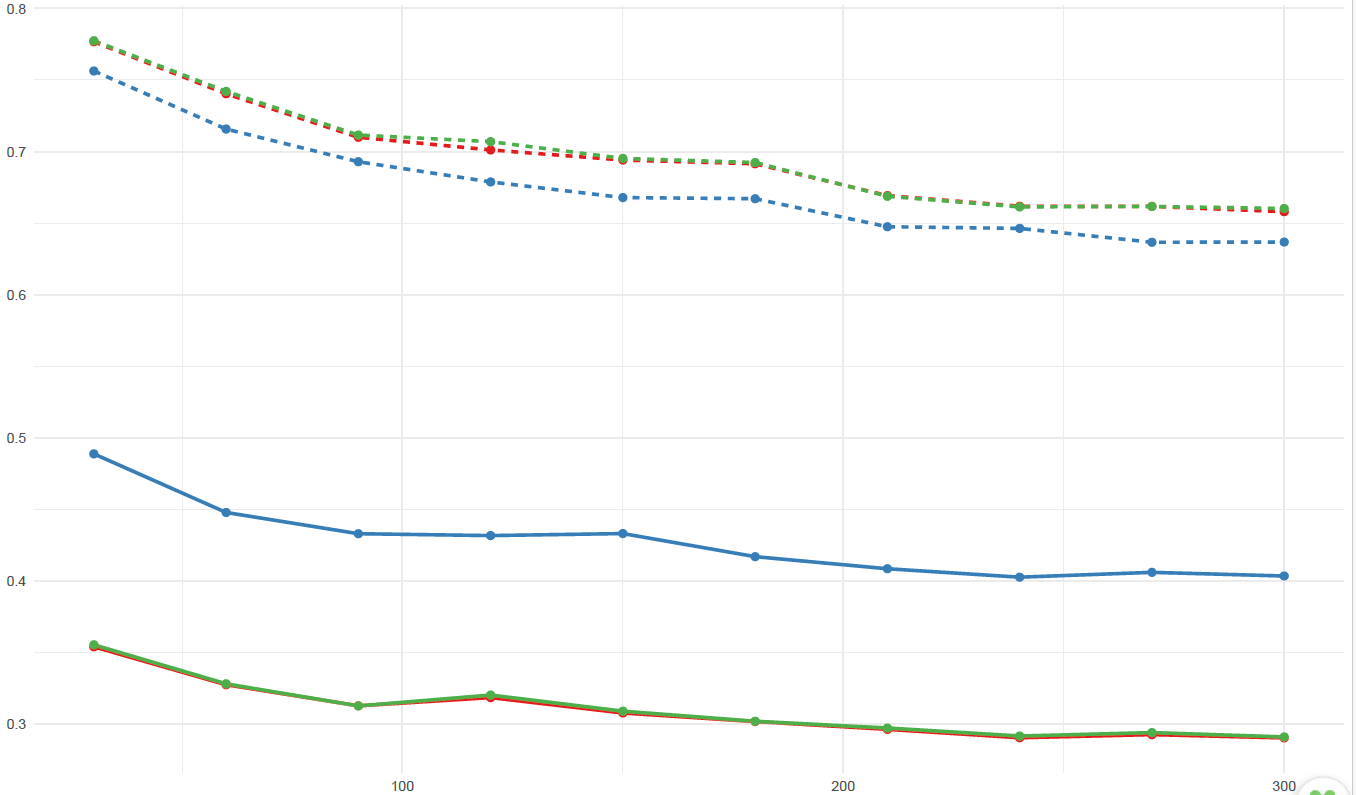
\includegraphics[width=0.75\linewidth]{Learning_curve.png}
    \caption{Aitchison distance as a function of training sample size for all three 
    Random Forest models.}
    \label{fig:enter-label}
\end{figure}
}
\end{frame}



\begin{frame}
\only<1>{
\note{I am not sure to include this slide:

And for further evaluation of \texttt{Dirichlet-RF}, we also looked at its performance in terms of covariate selection.

Here, you can see how often each covariate was selected for splitting across all trees, and how much, on average, it contributed to increasing the log-likelihood.

As I mentioned earlier, only three of the variables were informative — and \texttt{Dirichlet-RF} was able to clearly identify them with high importance.}
\begin{table}[htbp]
\centering
\begin{tabular}{|c|c|c|}
\hline
\textbf{Covariate} & \small{Log-Likelihood Importance} & \small{Frequency-Based Importance} \\
\hline
\textcolor{blue}{$X_1$} & \textcolor{blue}{225.039} & \textcolor{blue}{14} \\
\textcolor{blue}{$X_2$} & \textcolor{blue}{303.618} & \textcolor{blue}{21} \\
\textcolor{blue}{$X_3$} & \textcolor{blue}{272.036} & \textcolor{blue}{19} \\
\textcolor{red}{$X_4$} & \textcolor{red}{16.839}  & \textcolor{red}{2}  \\
\textcolor{red}{$X_5$} & \textcolor{red}{9.972}   & \textcolor{red}{2}  \\
\textcolor{red}{$X_6$} & \textcolor{red}{15.649}  & \textcolor{red}{3}  \\
\textcolor{red}{$X_7$} & \textcolor{red}{0}   & \textcolor{red}{0}  \\
\textcolor{red}{$X_8$} & \textcolor{red}{40.240}  & \textcolor{red}{6}  \\
\textcolor{red}{$X_9$} & \textcolor{red}{5.369}   & \textcolor{red}{1}  \\
\textcolor{red}{$X_{10}$} & \textcolor{red}{23.295}  & \textcolor{red}{3}  \\
\hline
\end{tabular}
\caption{Variable importance scores based on log-likelihood improvement and selection frequency, averaged across all trees in the \texttt{Dirichlet-RF}.}

\label{tab:variable-importance}
\end{table}
\note{
A noteworthy observation is that our model demonstrates effective Covariate selection capabilities through two complementary variable importance measures: log-likelihood importance, which quantifies each variable's contribution to model fit improvement, and frequency-based importance, which measures how often each variable is selected for splitting nodes. Both metrics are averaged across all trees in the random forest. Analysis shows that $X_1$, $X_2$, and $X_3$ receive the highest importance scores across both metrics, identifying them as the informative predictors in our simulation. The remaining variables ($X_4$ through $X_{10}$) receive substantially lower importance scores, confirming the model's ability to distinguish signal from noise.}
}
\end{frame}



\begin{frame}

    \only<1>{
  \note{This real-world dataset is based on a soil texture dataset from KwaZulu-Natal in South Africa. The dataset includes 685 samples, with three compositional parts: sand, silt, and clay. In addition, we used 120 covariates at a spatial resolution of 250 by 250 meters. These covariates include vegetation indices, elevation, precipitation, temperature, and other climate-related variables. The data comes from the Agricultural Research Council – Institute of Soil, Climate and Water.}
\frametitle{Real Data Application: Soil Texture}

\begin{itemize}
    \item \textbf{Data:} 685 samples. \textbf{Compositional parts:} sand, silt, clay. \textbf{120 covariates} at $250\,\text{m} \times 250\,\text{m}$ resolution, including vegetation indices, elevation, precipitation, temperature, and other climate variables.
    
    \item \textbf{Source:} Agricultural Research Council – Institute of Soil, Climate and Water (KwaZulu-Natal, South Africa)
\end{itemize}}
    
    \only<2>{\frametitle{Comparison result}

    \note{\textbf{Dirichlet-RF} outperformed \textbf{CLR-RF} and \textbf{ILR-RF} across all evaluation metrics in this real-data example.

We also compared these models on many simulated datasets. Although we obtained better results in several cases, we cannot claim that this model will always outperform transformation-based Random Forest models in every situation. However, it can be considered a strong and well-structured model for compositional data.}
\begin{table}[ht]
\centering
\begin{tabular}{rrrrr}
  \hline
 & RF-CLR & RF-ILR  & \textcolor{blue}{\texttt{Dirichlet-RF}} \\ 
  \hline
aitchison distance & 1.08 & 1.08  & \textcolor{blue}{\textbf{0.98}} \\ 
  clayRMSE & 20.09 & 20.14  & \textcolor{blue}{\textbf{17.85}} \\ 
  siltRMSE & 13.94 & 13.91  & \textcolor{blue}{\textbf{12.41}} \\ 
  sandRMSE & 29.79 & 29.83  & \textcolor{blue}{\textbf{25.93}} \\ 
  meanRMSE & 22.25 & 22.28  & \textcolor{blue}{\textbf{19.54}} \\ 
   \hline
\end{tabular}
\caption{Results of \texttt{Dirichlet-RF}, \texttt{ILR-RF}, \texttt{CLR-RF}, and an RF without the use of a transformation on the soil texture data in KwaZulu-Natal in South Africa.}
\label{tab:real_results}
\end{table}

    }
\end{frame}





\begin{frame}{Implementation \& Code Access}
\note{This model was developed in Julia, and the full code is available on GitHub at the link provided.

We chose Julia mainly because of its strong computational performance. Implementing the model directly in R or Python would be much slower.

However, if you're working in R or Python, you can still use the model by calling the Julia functions from those languages.
We've included clear instructions in the repository, especially on how to connect Julia with R.

We're also planning to develop an R package with a C++ backend, which we hope to submit to CRAN, so the model will be even easier for R users to access.}
\vspace{1em}

\begin{itemize}[itemsep=1em]
\item[\textcolor{blue}{\large$\blacktriangleright$}] Model developed in \textbf{Julia} for computational efficiency

\item[\textcolor{blue}{\large$\blacktriangleright$}] Code available on \href{https://github.com/Xaleed/DirichletRandomForestJulia.git}{\textcolor{blue}{\textbf{GitHub}}}:

\textcolor{blue}{\small{https://github.com/Xaleed/DirichletRandomForestJulia.git}}
  \begin{center}

    \qrcode{https://github.com/Xaleed/DirichletRandomForestJulia.git}
 \end{center}
\item[\textcolor{blue}{\large$\blacktriangleright$}] Not suitable for direct implementation in \textbf{R} or \textbf{Python}.
However, Julia functions can be called from R or Python.

\end{itemize}

\vspace{1.5em}

\end{frame}

\begin{frame}{}
\only<1>{
\note{One important disadvantage of this approach is the computational cost of estimating the maximum likelihood parameters.

Because there’s no closed-form solution for the maximum likelihood estimator of the Dirichlet distribution parameters we have to solve it numerically.

For example, if we have 10 covariates and 10 candidate split points per covariate, that means we need to numerically solve the MLE problem 600 times at each node.}
\centering
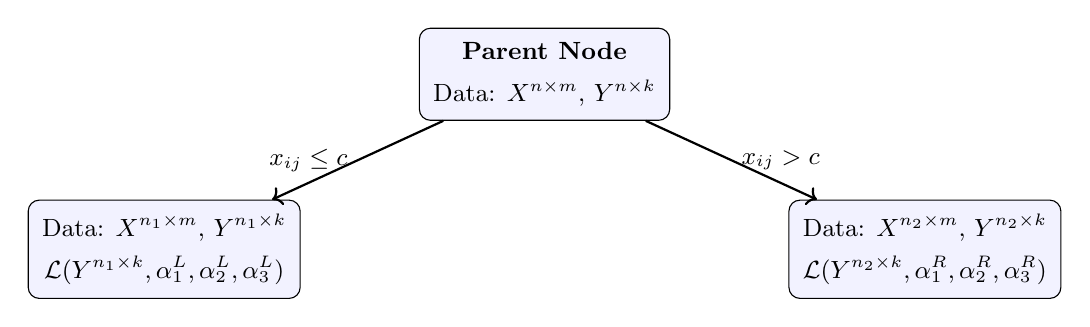
\begin{tikzpicture}[
  node distance=1cm and 1.5cm,
  every node/.style={font=\small},
  data/.style={rectangle, draw, align=center, fill=blue!5, rounded corners, inner sep=5pt},
  split/.style={->, thick}
  ]
  % Parent node
  \node[data] (parent) {
    \textbf{Parent Node} \\[0.15cm]
    Data: $X^{n \times m}$, $Y^{n \times k}$
  };
  
  % Left child
  \node[data, below left=of parent] (left) {
    Data: $X^{n_1 \times m}$, $Y^{n_1 \times k}$ \\[0.15cm]
    $\mathcal{L}(Y^{n_1 \times k}, \alpha_1^L, \alpha_2^L, \alpha_3^L)$
  };
  
  % Right child
  \node[data, below right=of parent] (right) {
    Data: $X^{n_2 \times m}$, $Y^{n_2 \times k}$ \\[0.15cm]
    $\mathcal{L}(Y^{n_2 \times k}, \alpha_1^R, \alpha_2^R, \alpha_3^R)$
  };
  
  % Arrows
  \draw[split] (parent) -- node[midway, left] {$x_{ij} \leq c$} (left);
  \draw[split] (parent) -- node[midway, right] {$x_{ij} > c$} (right);
\end{tikzpicture}

\vspace{0.5cm}



\[
(i^*, c^*) = \operatorname{argmax}_{i,c} \left( \max_{\boldsymbol{\alpha}^L} \mathcal{L}(Y^{n_1 \times k}, \boldsymbol{\alpha}^L) + \max_{\boldsymbol{\alpha}^R} \mathcal{L}(Y^{n_2 \times k}, \boldsymbol{\alpha}^R) \right)
\]
\textbf{Parameter Estimation Complexity:} $6 \times m \times p$ parameters per split:
\[
\text{Total = }6 \times m \times p =  6 \times 10 \times 10 = 600 \text{ optimizations per node}
\]
}
% \only<2>{
% For trees that can potentially grow in all directions to at least 6 levels deep, we have:
% \begin{equation}
% 3 \times m \times p \times \sum_{i=1}^{6} 2^i = 3 \times m \times p \times 126 = 378 \times m \times p
% \end{equation}
% parameters that we estimate dynamically. This number can become very large---for example, when $m=10$ and $p=10$, the total number of parameters is $378 \times 10 \times 10 = 37,800$.
% }
\only<2>{
\note{If we build a tree with just three levels — meaning a tree with 8 leaves — we already need to solve the optimization problem 4,200 times.

This is a large computational cost. And remember, trees can grow much deeper depending on the dataset. As the depth increases, the number of nodes — and therefore the number of parameter estimations — grows exponentially.}
    \centering
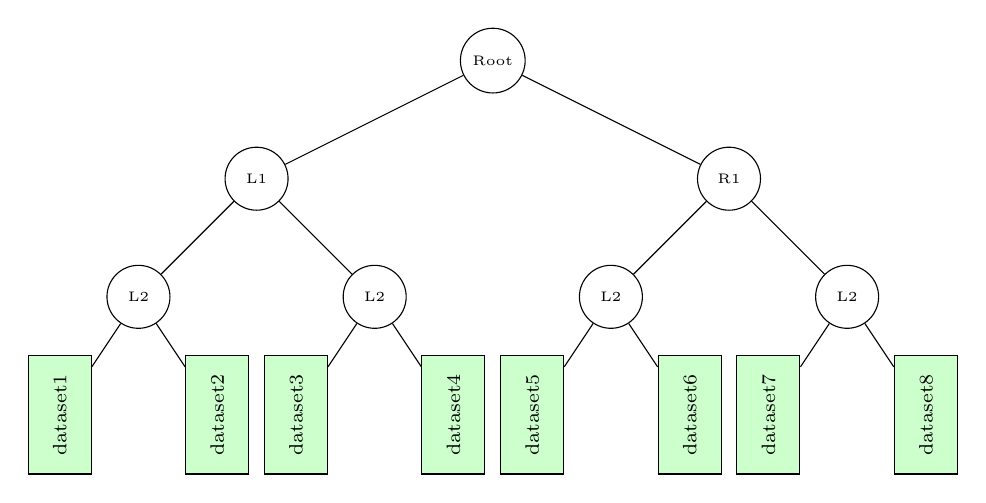
\begin{tikzpicture}[
  level/.style={sibling distance=60mm/#1},
  every node/.style={circle, draw, minimum size=8mm, font=\tiny},
  leaf/.style={rectangle, draw, fill=green!20, minimum width=15mm, minimum height=8mm, font=\scriptsize, rotate=90}
]
\node {Root}
  child {
    node {L1}
    child {
      node {L2}
      child {
        node[leaf] {dataset1}
      }
      child {
        node[leaf] {dataset2}
      }
    }
    child {
      node {L2}
      child {
        node[leaf] {dataset3}
      }
      child {
        node[leaf] {dataset4}
      }
    }
  }
  child {
    node {R1}
    child {
      node {L2}
      child {
        node[leaf] {dataset5}
      }
      child {
        node[leaf] {dataset6}
      }
    }
    child {
      node {L2}
      child {
        node[leaf] {dataset7}
      }
      child {
        node[leaf] {dataset8}
      }
    }
  };
\end{tikzpicture}

With $10$ covariates and $10$ candidates per covariate, the model requires $3 \times 10\times 10 \times (2+2^2+2^3) = 4200$ parameters, all estimated using maximum likelihood estimation. As the tree depth increases, the parameter count grows exponentially.
\note{
This tree diagram illustrates a hierarchical model designed to generate 8 subdatasets, each following a Dirichlet distribution. With 10 covariates and 10 candidates per covariate, the model requires 10×10×(2+2²+2³) = 1,400 parameters, all estimated using maximum likelihood estimation. As the tree depth increases, the parameter count grows exponentially.}
}
% \only<4>{

%  This large parameter space provides the model with sufficient flexibility to accommodate diverse datasets, addressing a key limitation of traditional methods related to the Dirichlet distribution, like Dirichlet regression methods for compositional data analysis. However, this flexibility comes at a significant computational cost, rendering the approach impractical for large-scale datasets. 
% }
% \only<3>{
% The discussion of computational performance remains a significant issue for big datasets in our methodology. We have identified several promising directions for future research and performance improvements. As we discussed, MoM works well as an alternative to MLE, providing good approximations with higher computational speed. We can combine these estimation methods by selectively replacing MLE with MoM in specific nodes where we can predict the results of both methods would be similar, rather than applying MoM to all nodes.
% }
\end{frame}
\begin{frame}{Alternative to MLE}
    \only<1>{
    \begin{block}{}
        One simple way to address this issue is to use the method of moments (MoM) as an alternative to maximum likelihood estimation (MLE). MoM gives an approximate solution but is much faster to compute.
    \end{block}
     \begin{block}{}
        We can also combine both approaches — instead of using MoM in all nodes, we can selectively apply it only in nodes where we expect its results to be close to MLE. This helps reduce computation while still keeping good accuracy.
    \end{block}
            \resizebox{0.65\linewidth}{!}{%

\begin{table}[htbp]
\centering

\begin{tabular}{|l|c|c|c|c|}
\hline
\multirow{Metric} & \multicolumn{2}{c|}{MLE} & \multicolumn{2}{c|}{MoM} \\
\cline{2-5}
 & (Train) & (Test) & (Train) & (Test) \\
\hline
Aitchison Distance & 0.3901 & 0.7391 & 0.4068 & 0.7457 \\
\hline
\end{tabular}
\end{table}}



}
\end{frame}


% \begin{frame}[plain]
% % \begin{center}
% %    
\includegraphics[width=5cm]{logo.png} % Optional logo
% %    \end{center}
%   \begin{center}
%       \vspace{2cm}

%     {\Huge \textbf{Thank You!} \par}
%     % \vspace{1cm}
%     % {\Large Questions or Comments? \par}
%     \vspace{1cm}
   
    
%     \qrcode{https://github.com/Xaleed/DirichletRandomForestJulia.git}
%    % \texttt{khaledmasoumifard@sun.ac.za}
%   \end{center}
% \end{frame}





%


%% ─── SLIDE 1: Study Area & Data ───────────────────────────────────────────
\begin{frame}{ Data}

\begin{itemize}[label=\textbullet]
    \item We use soil texture data from Germany. The data comes from the 2018 LUCAS survey.
    
    \vspace{0.5em}
    
    \item We have around 1,785 observations. Each observation contains three components: clay, sand, and silt — and together they always sum to one, which makes this compositional data.
    

  
    
    \vspace{0.5em}
    
    \item A total of \textbf{133 environmental covariates} (at $250 \times 250$ m resolution) were used as predictors, including climate, temperature, and vegetation-related variables.
    
    \vspace{0.5em}
   
\end{itemize}

\end{frame}


% %% ─── SLIDE 2: Spatial Patterns ─────────────────────────────────────────────
% \begin{frame}{Spatial Distribution of Soil Texture}

% \begin{figure}
%     \centering
%     \begin{columns}
%         \begin{column}{0.33\textwidth}
%             \centering
%             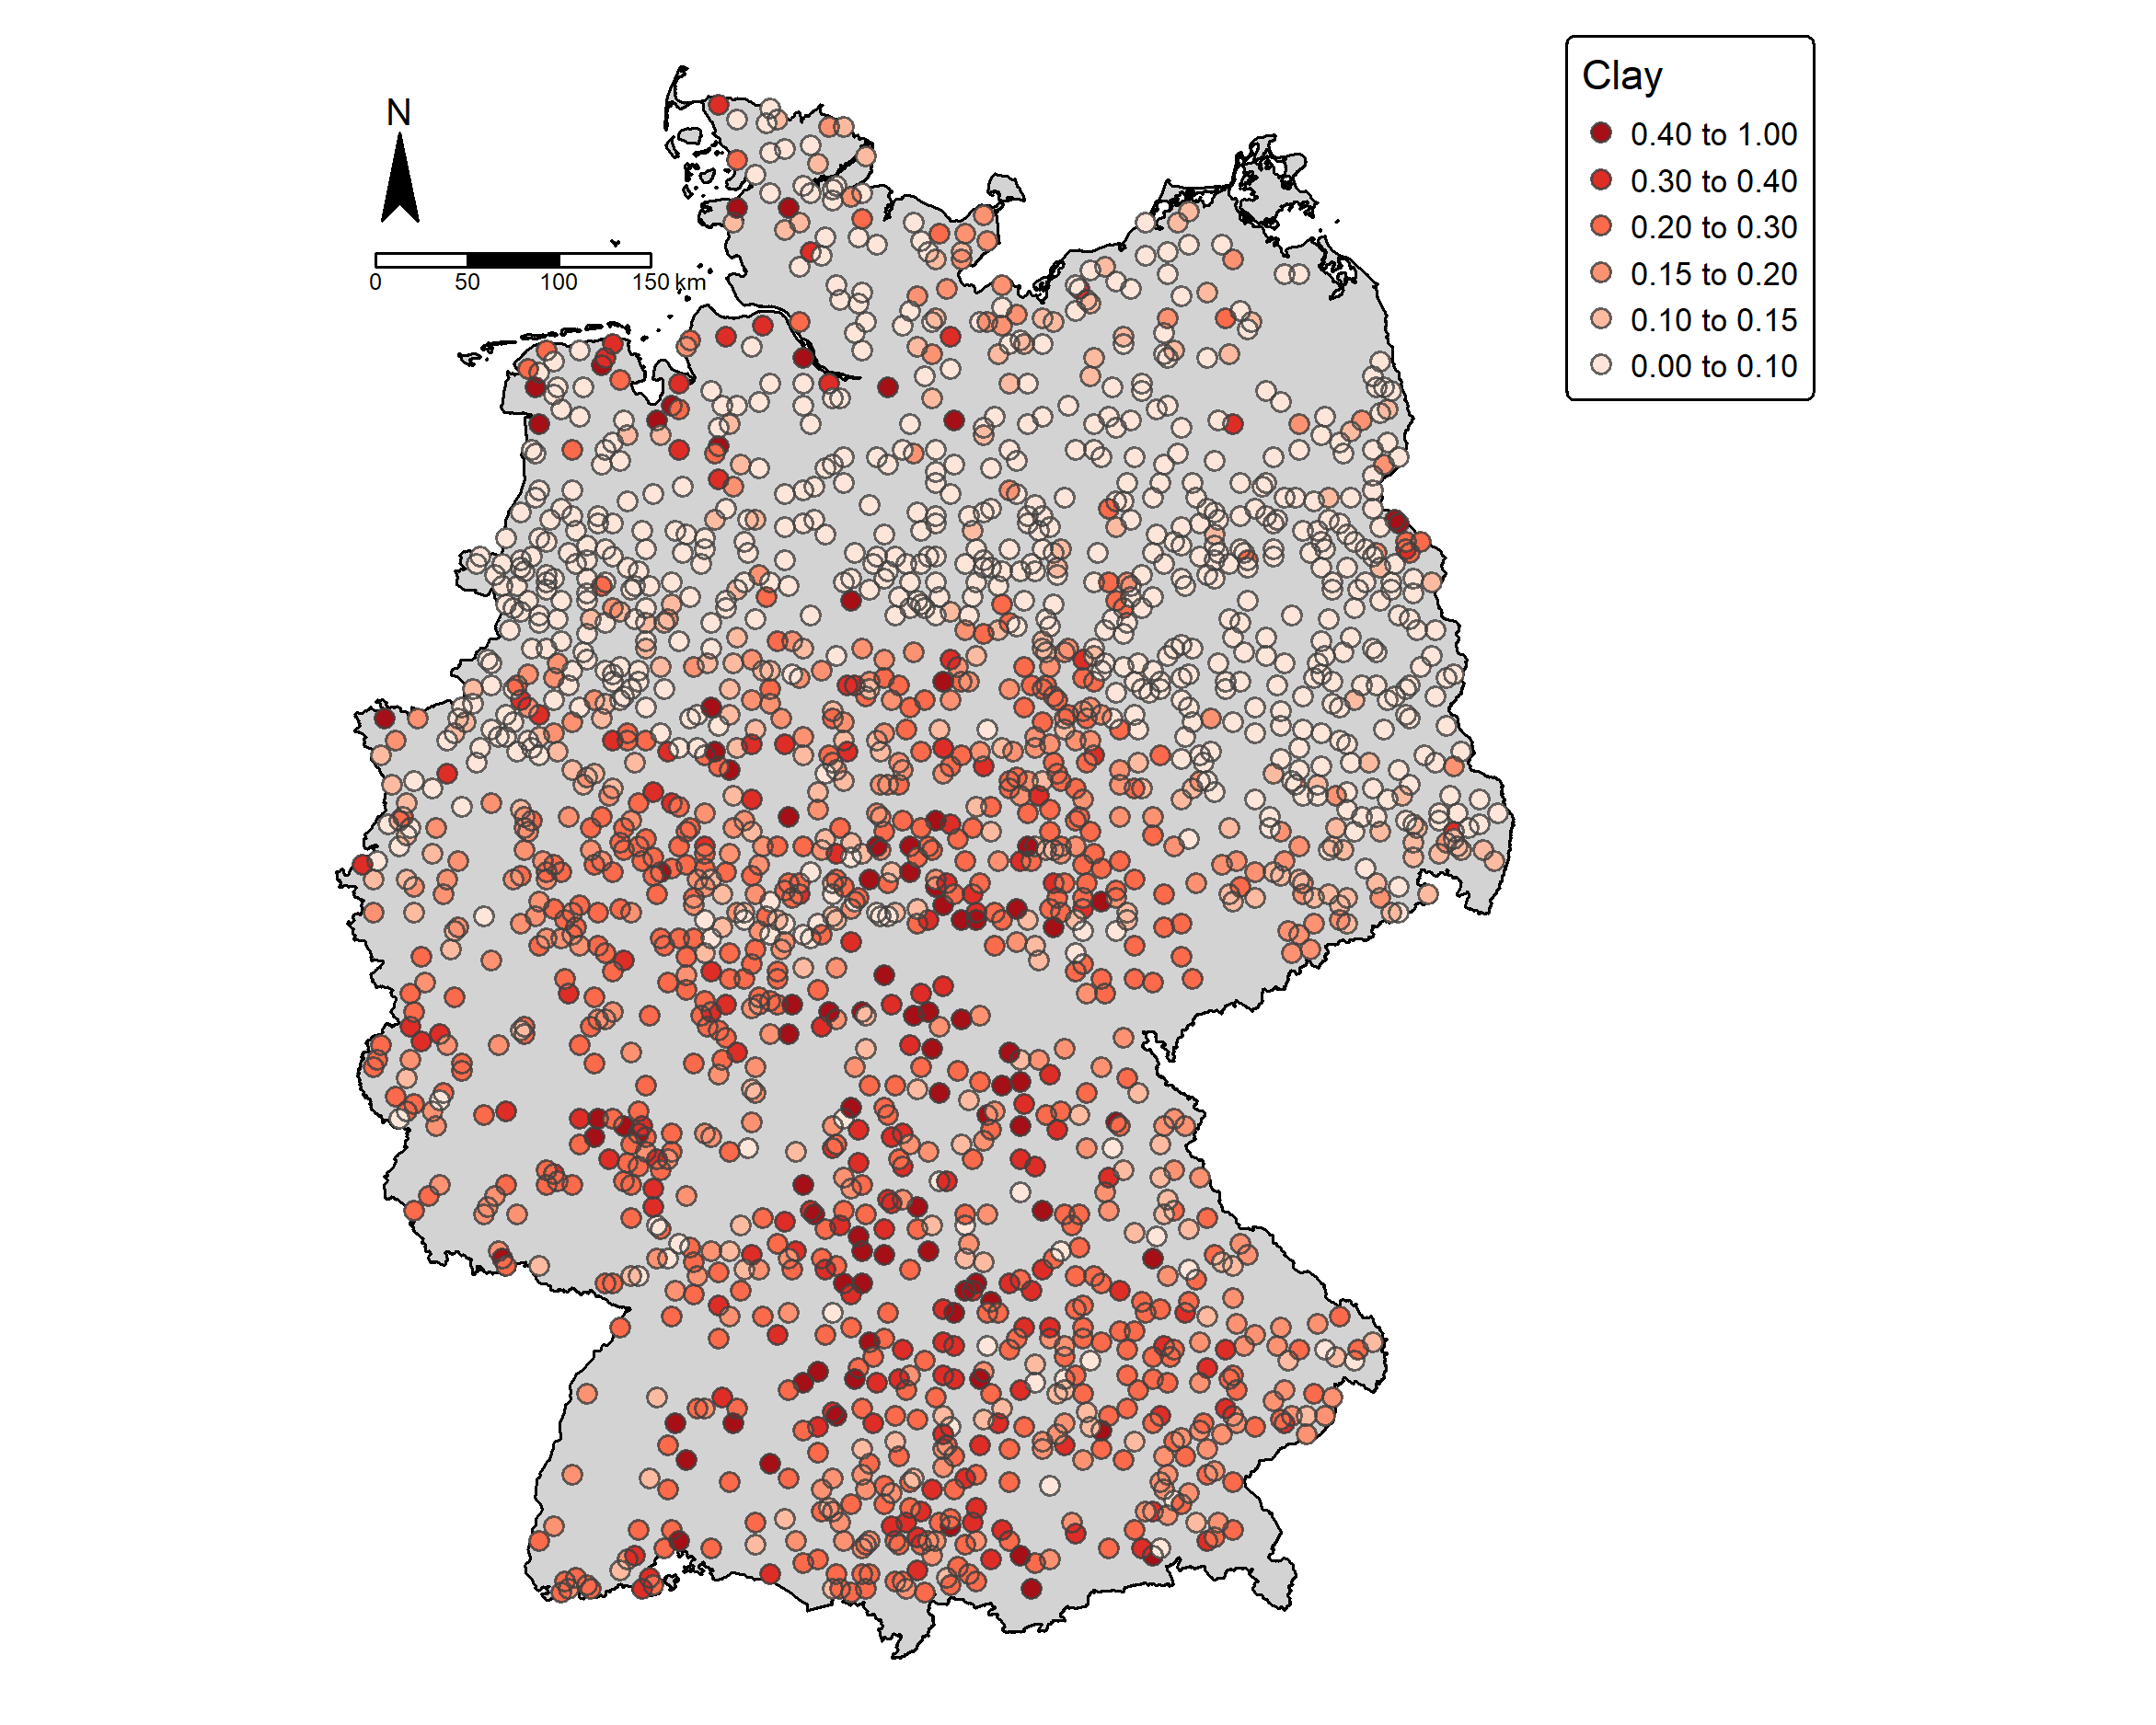
\includegraphics[width=\linewidth]{Figures/pointmap_clay.png}
%             \\ (a) Clay
%         \end{column}
%         \begin{column}{0.33\textwidth}
%             \centering
%             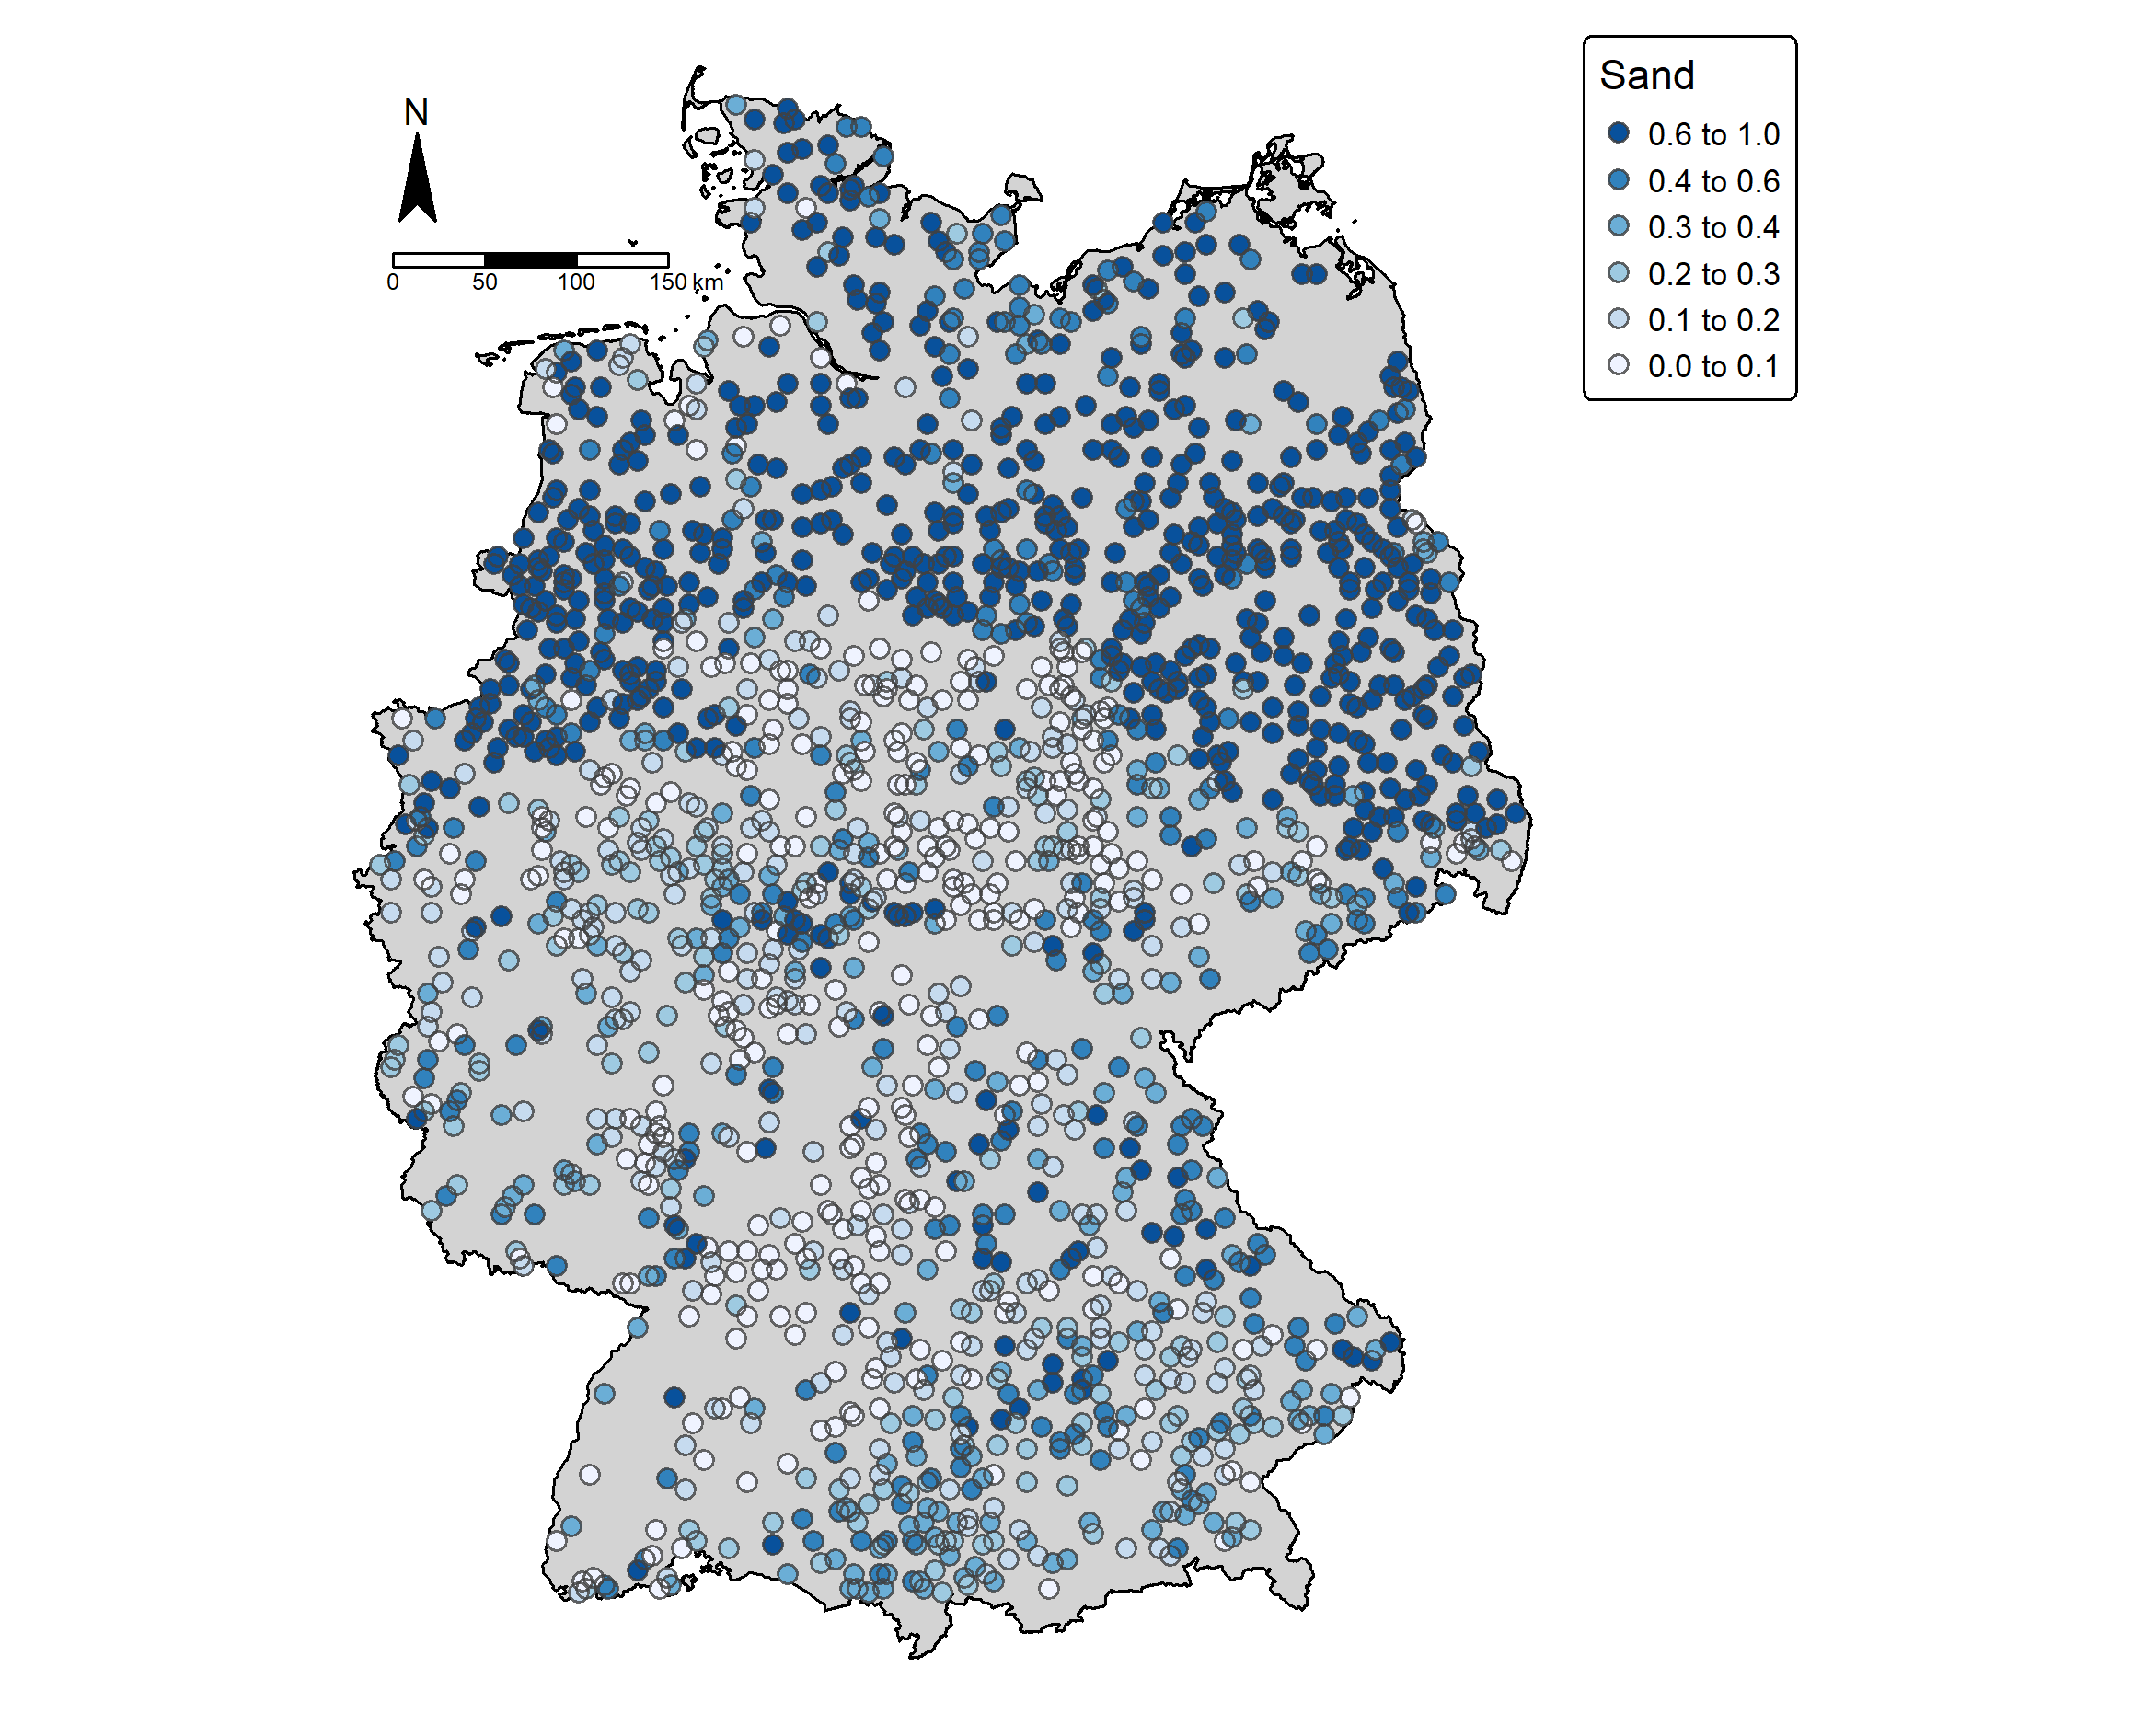
\includegraphics[width=\linewidth]{Figures/pointmap_sand.png}
%             \\ (b) Sand
%         \end{column}
%         \begin{column}{0.33\textwidth}
%             \centering
%             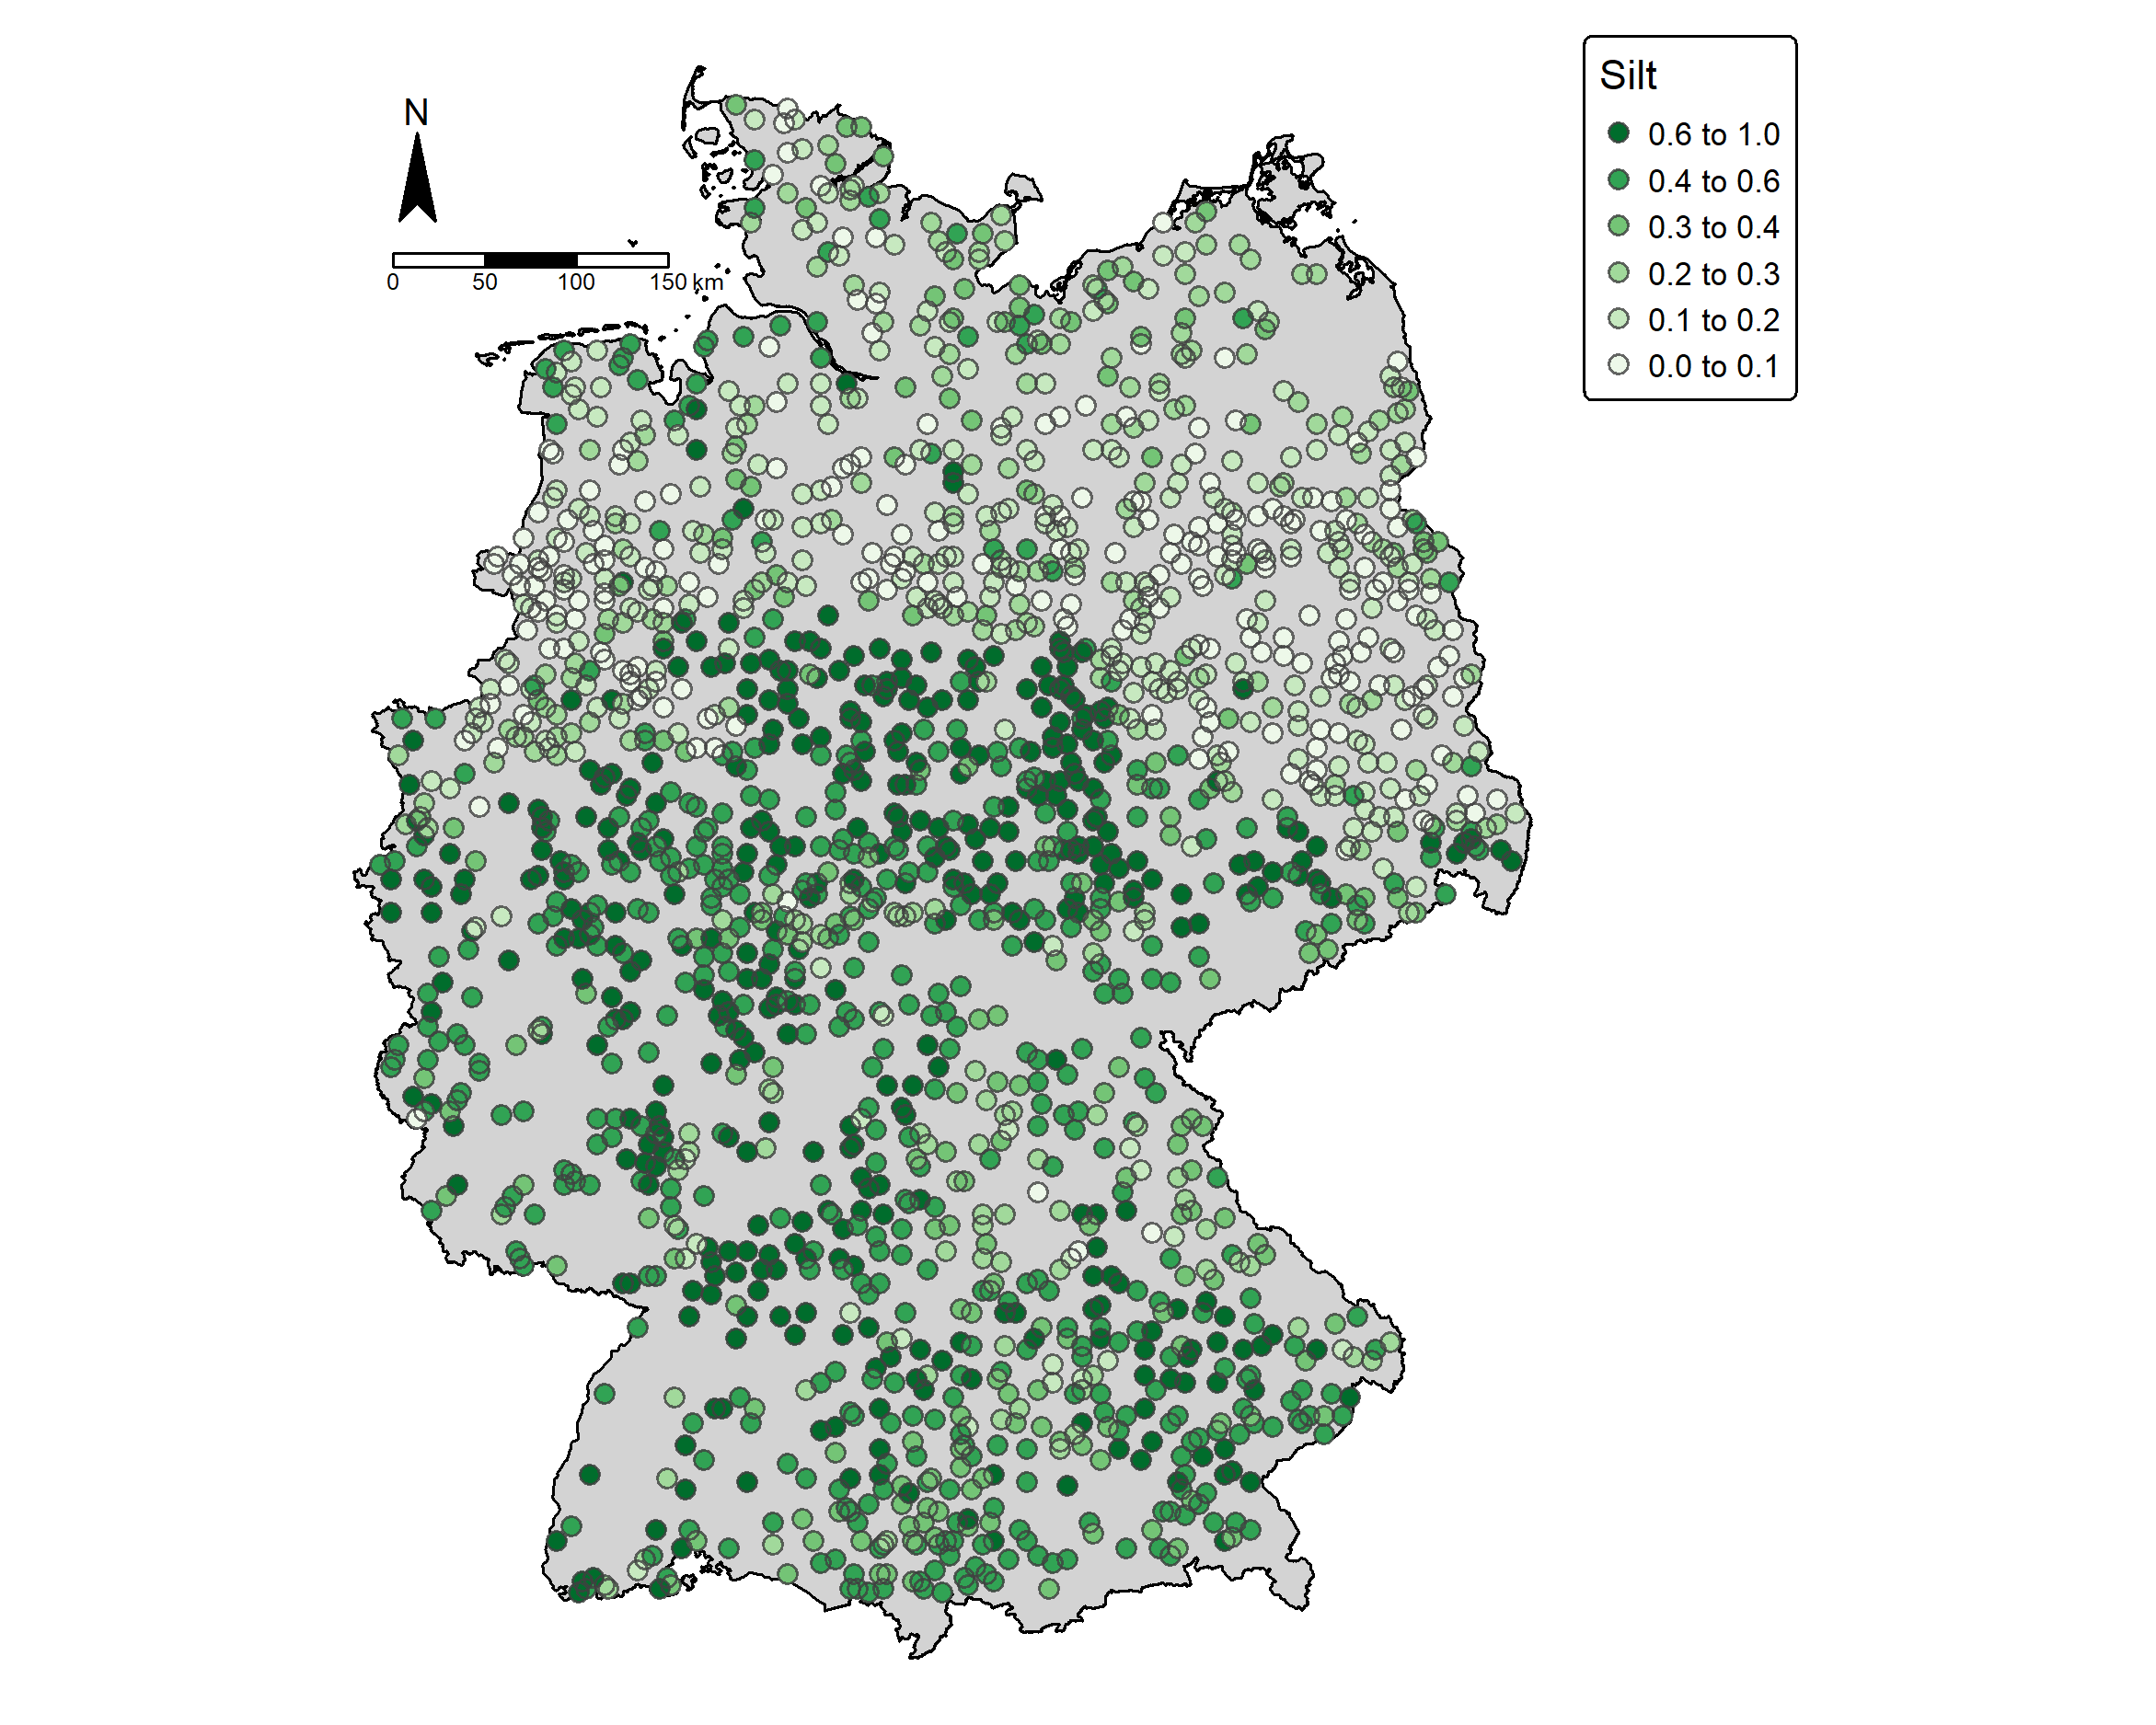
\includegraphics[width=\linewidth]{Figures/pointmap_silt.png}
%             \\ (c) Silt
%         \end{column}
%     \end{columns}
%     \caption{LUCAS soil texture observation locations in Germany: (a) Clay, (b) Sand, (c) Silt (shown as proportions).}
% \end{figure}

% \end{frame}

%% ─── SLIDE 2: Spatial Patterns ─────────────────────────────────────────────
\begin{frame}{Spatial Distribution of Soil Texture}

\begin{columns}

    \begin{column}{0.45\textwidth}
        \begin{itemize}
            \item[1.] Each point represents one \textbf{observation location} in Germany.
            
            \item[2.] The \textbf{colour} of each point indicates the value of the component: darker colours indicate \textbf{higher values}, lighter colours indicate \textbf{lower values}.
            
            \item[3.] \textbf{Clay:} higher values concentrated in the \textbf{south and centre}.
            
            \item[5.] \textbf{Sand:} higher values mostly in the \textbf{north and north-east}.
            
            \item[6.] \textbf{Silt:} more mixed pattern, with elevated values across the \textbf{central belt}.
        \end{itemize}
    \end{column}

    \begin{column}{0.55\textwidth}
        \only<1>{
        \begin{figure}
            \centering
            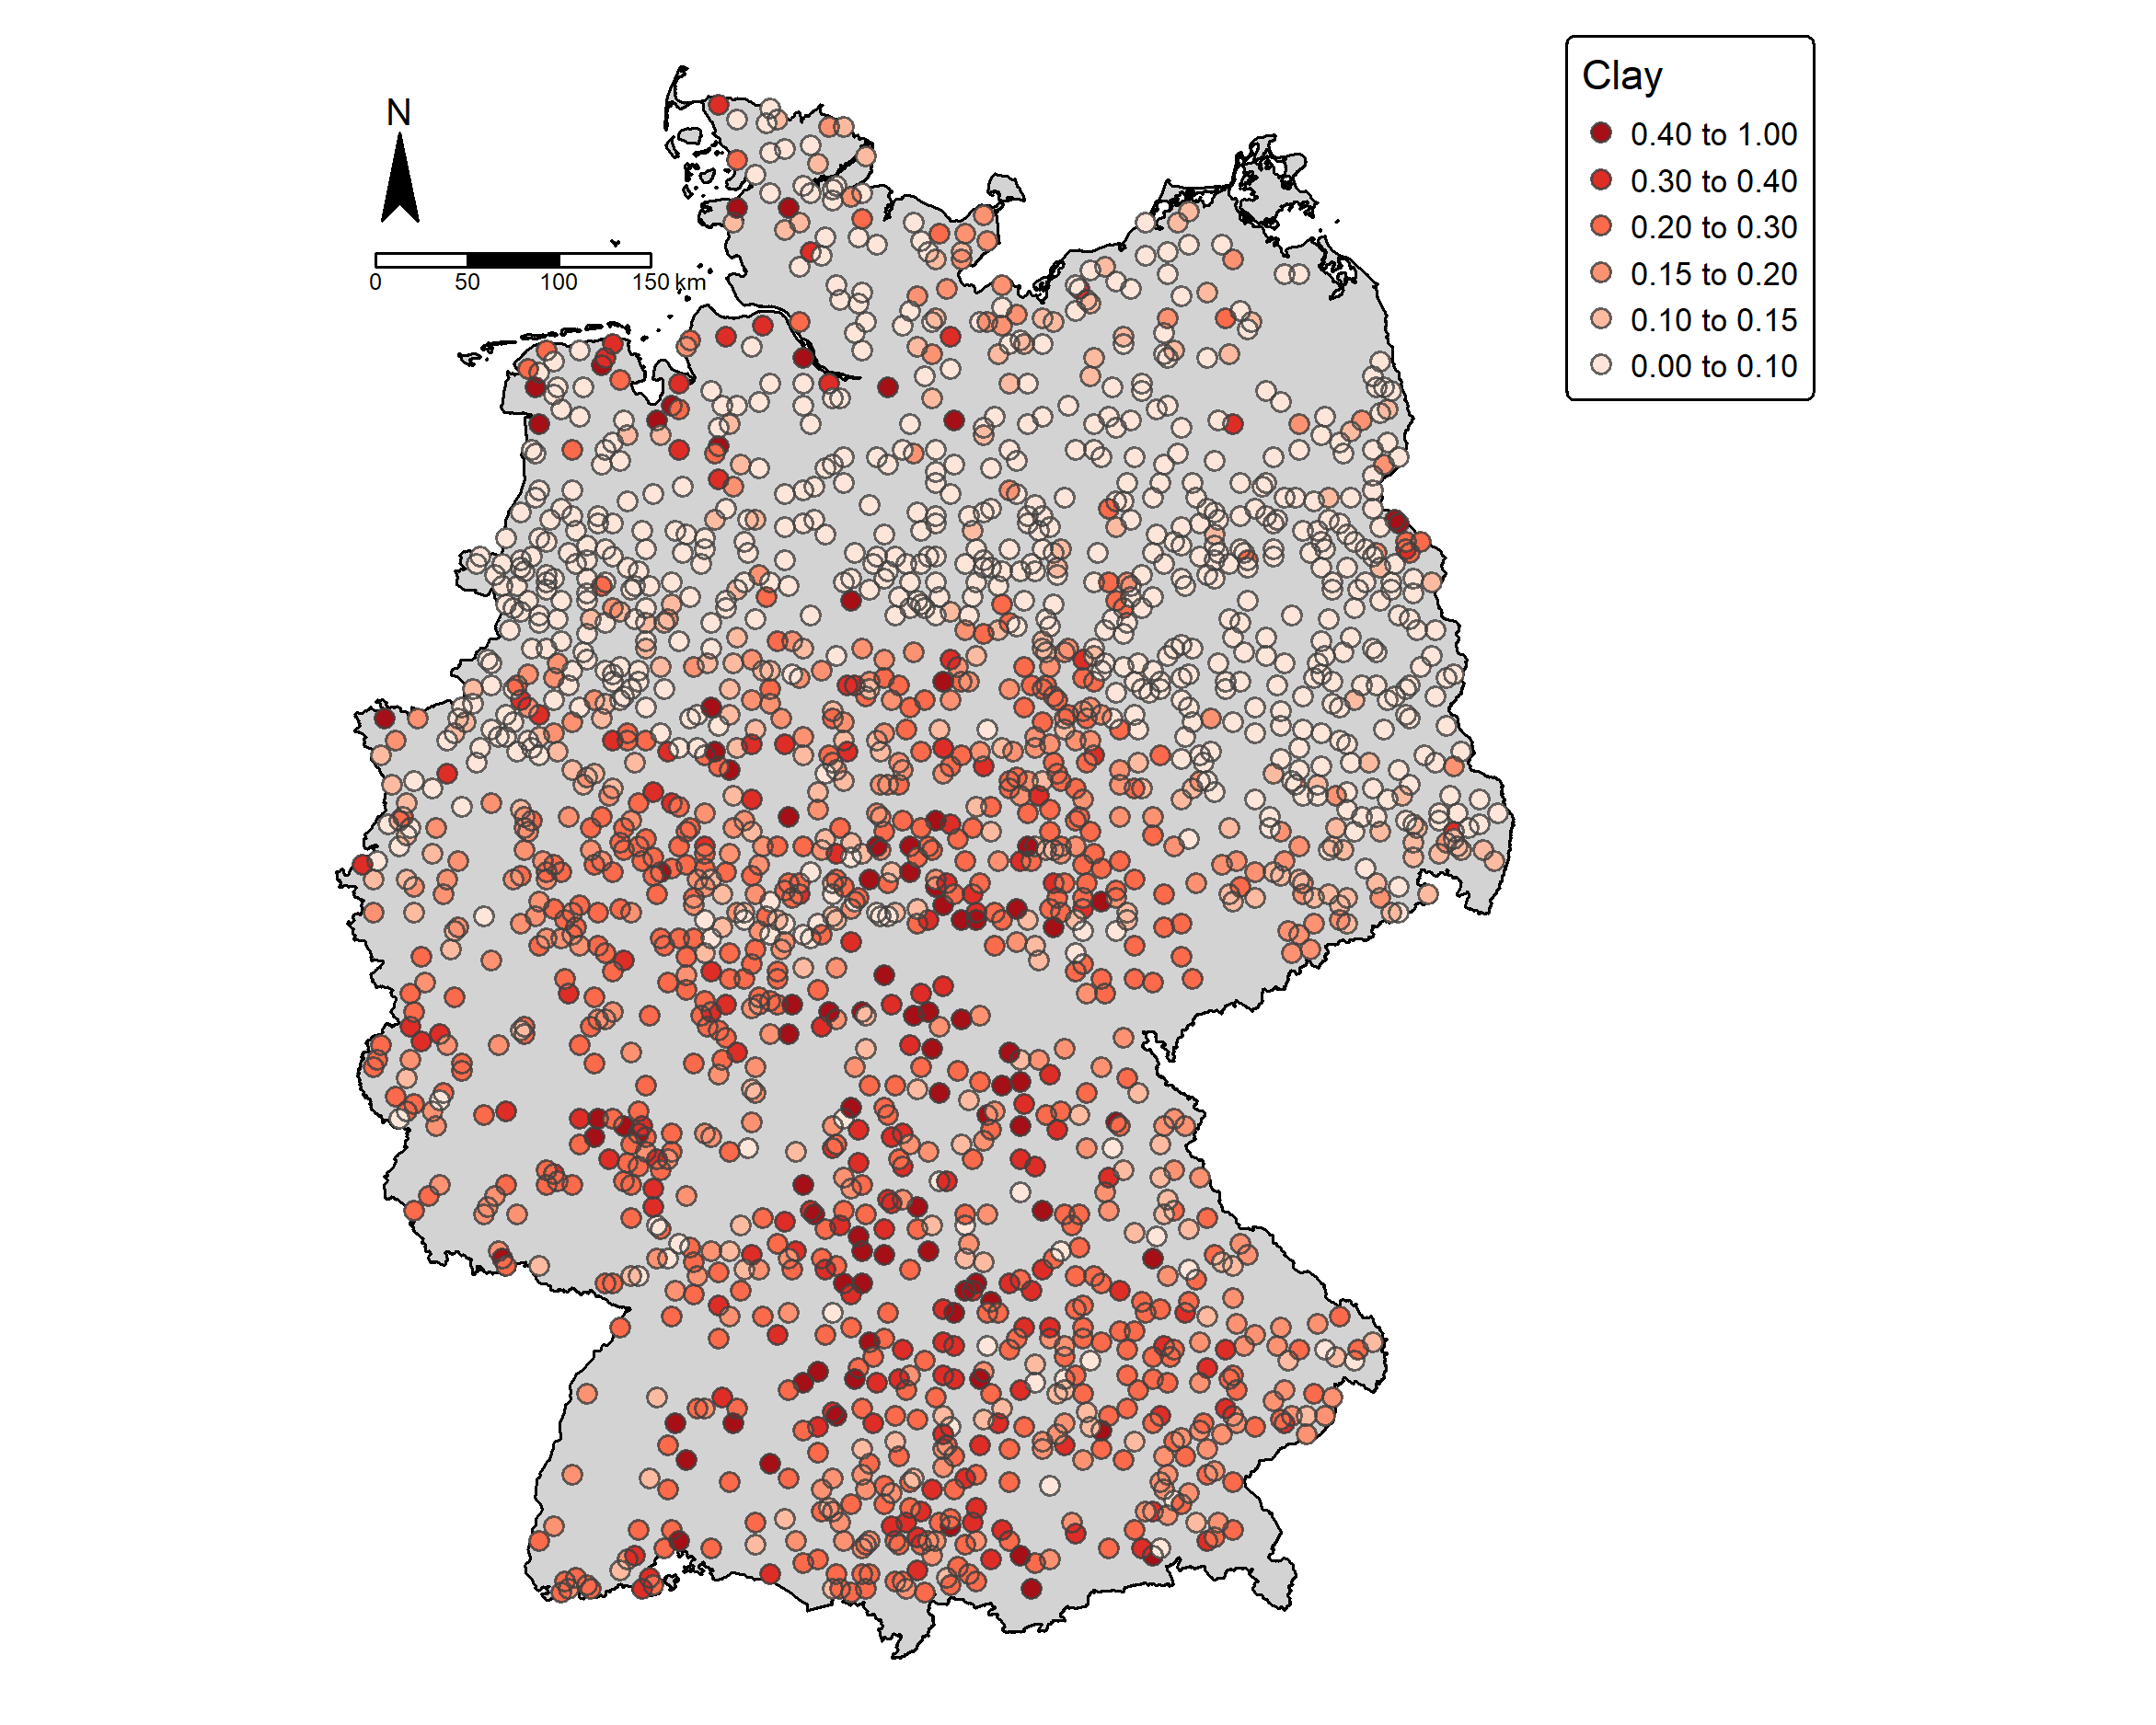
\includegraphics[width=\linewidth]{Figures/pointmap_clay.png}
            \caption{LUCAS soil texture observation locations in Germany: Clay.}
        \end{figure}}
        \only<2>{
        \begin{figure}
            \centering
            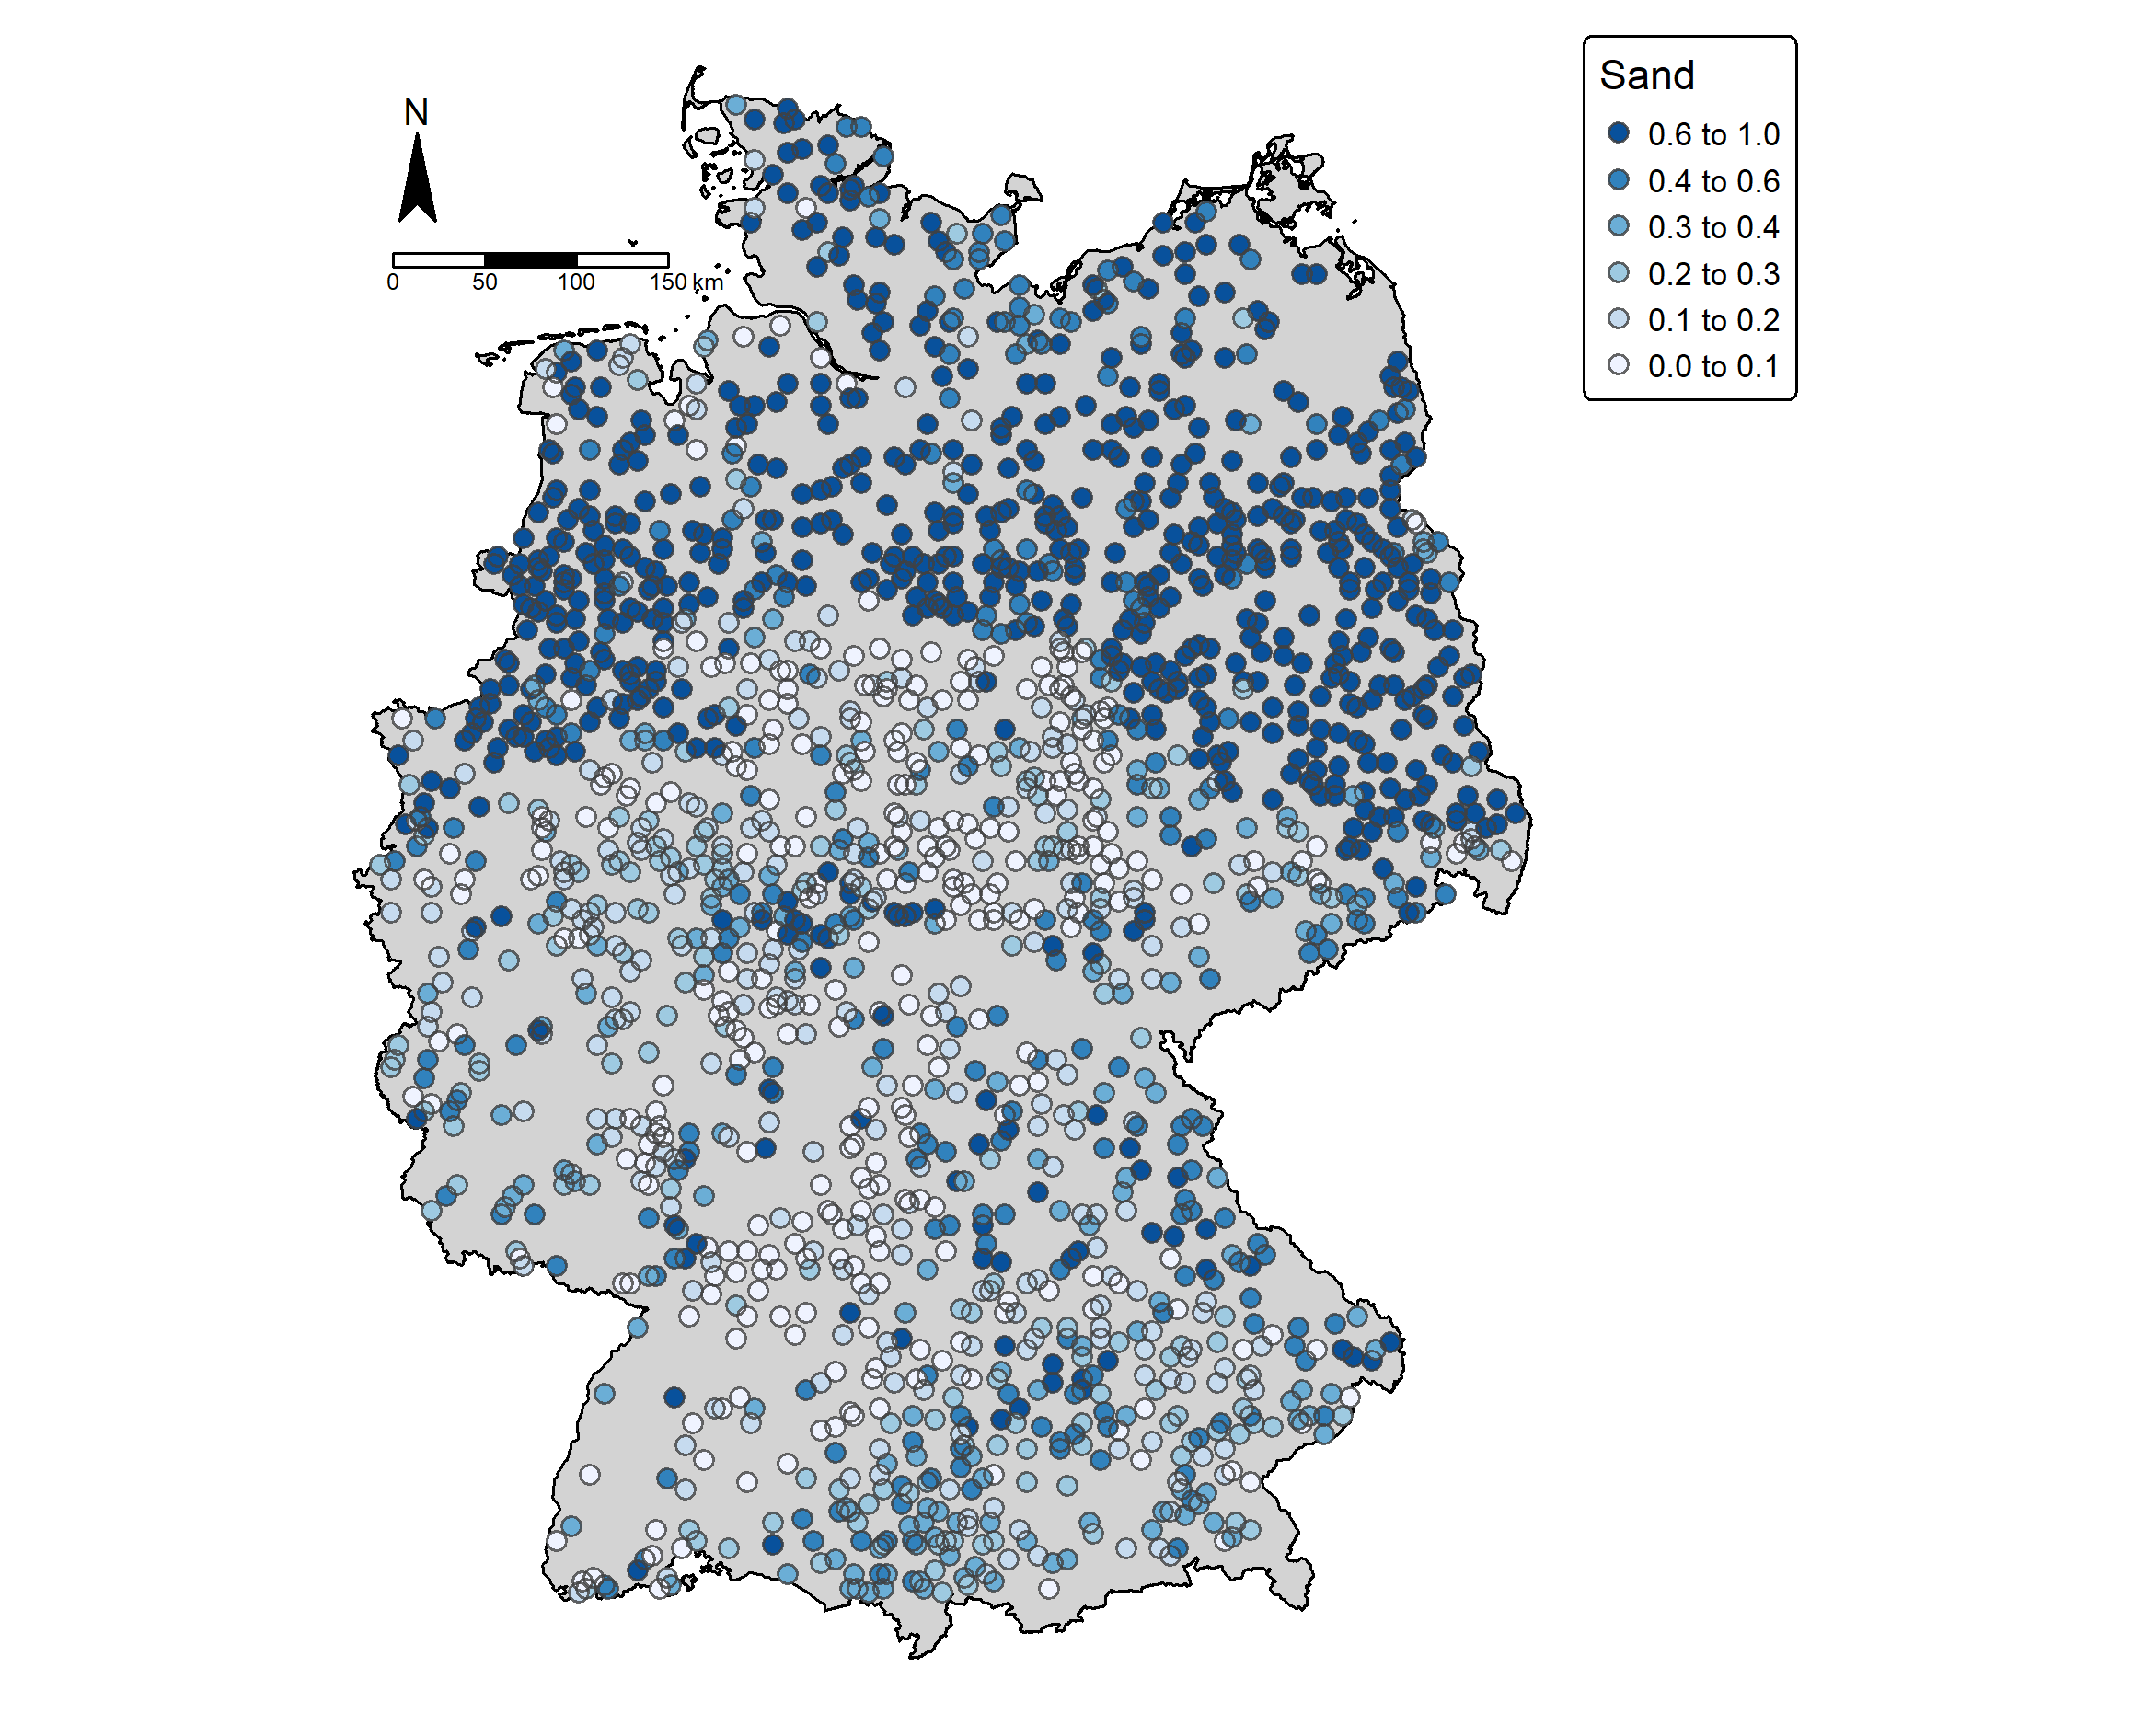
\includegraphics[width=\linewidth]{Figures/pointmap_sand.png}
            \caption{LUCAS soil texture observation locations in Germany: Sand.}
        \end{figure}}
        \only<3>{
        \begin{figure}
            \centering
            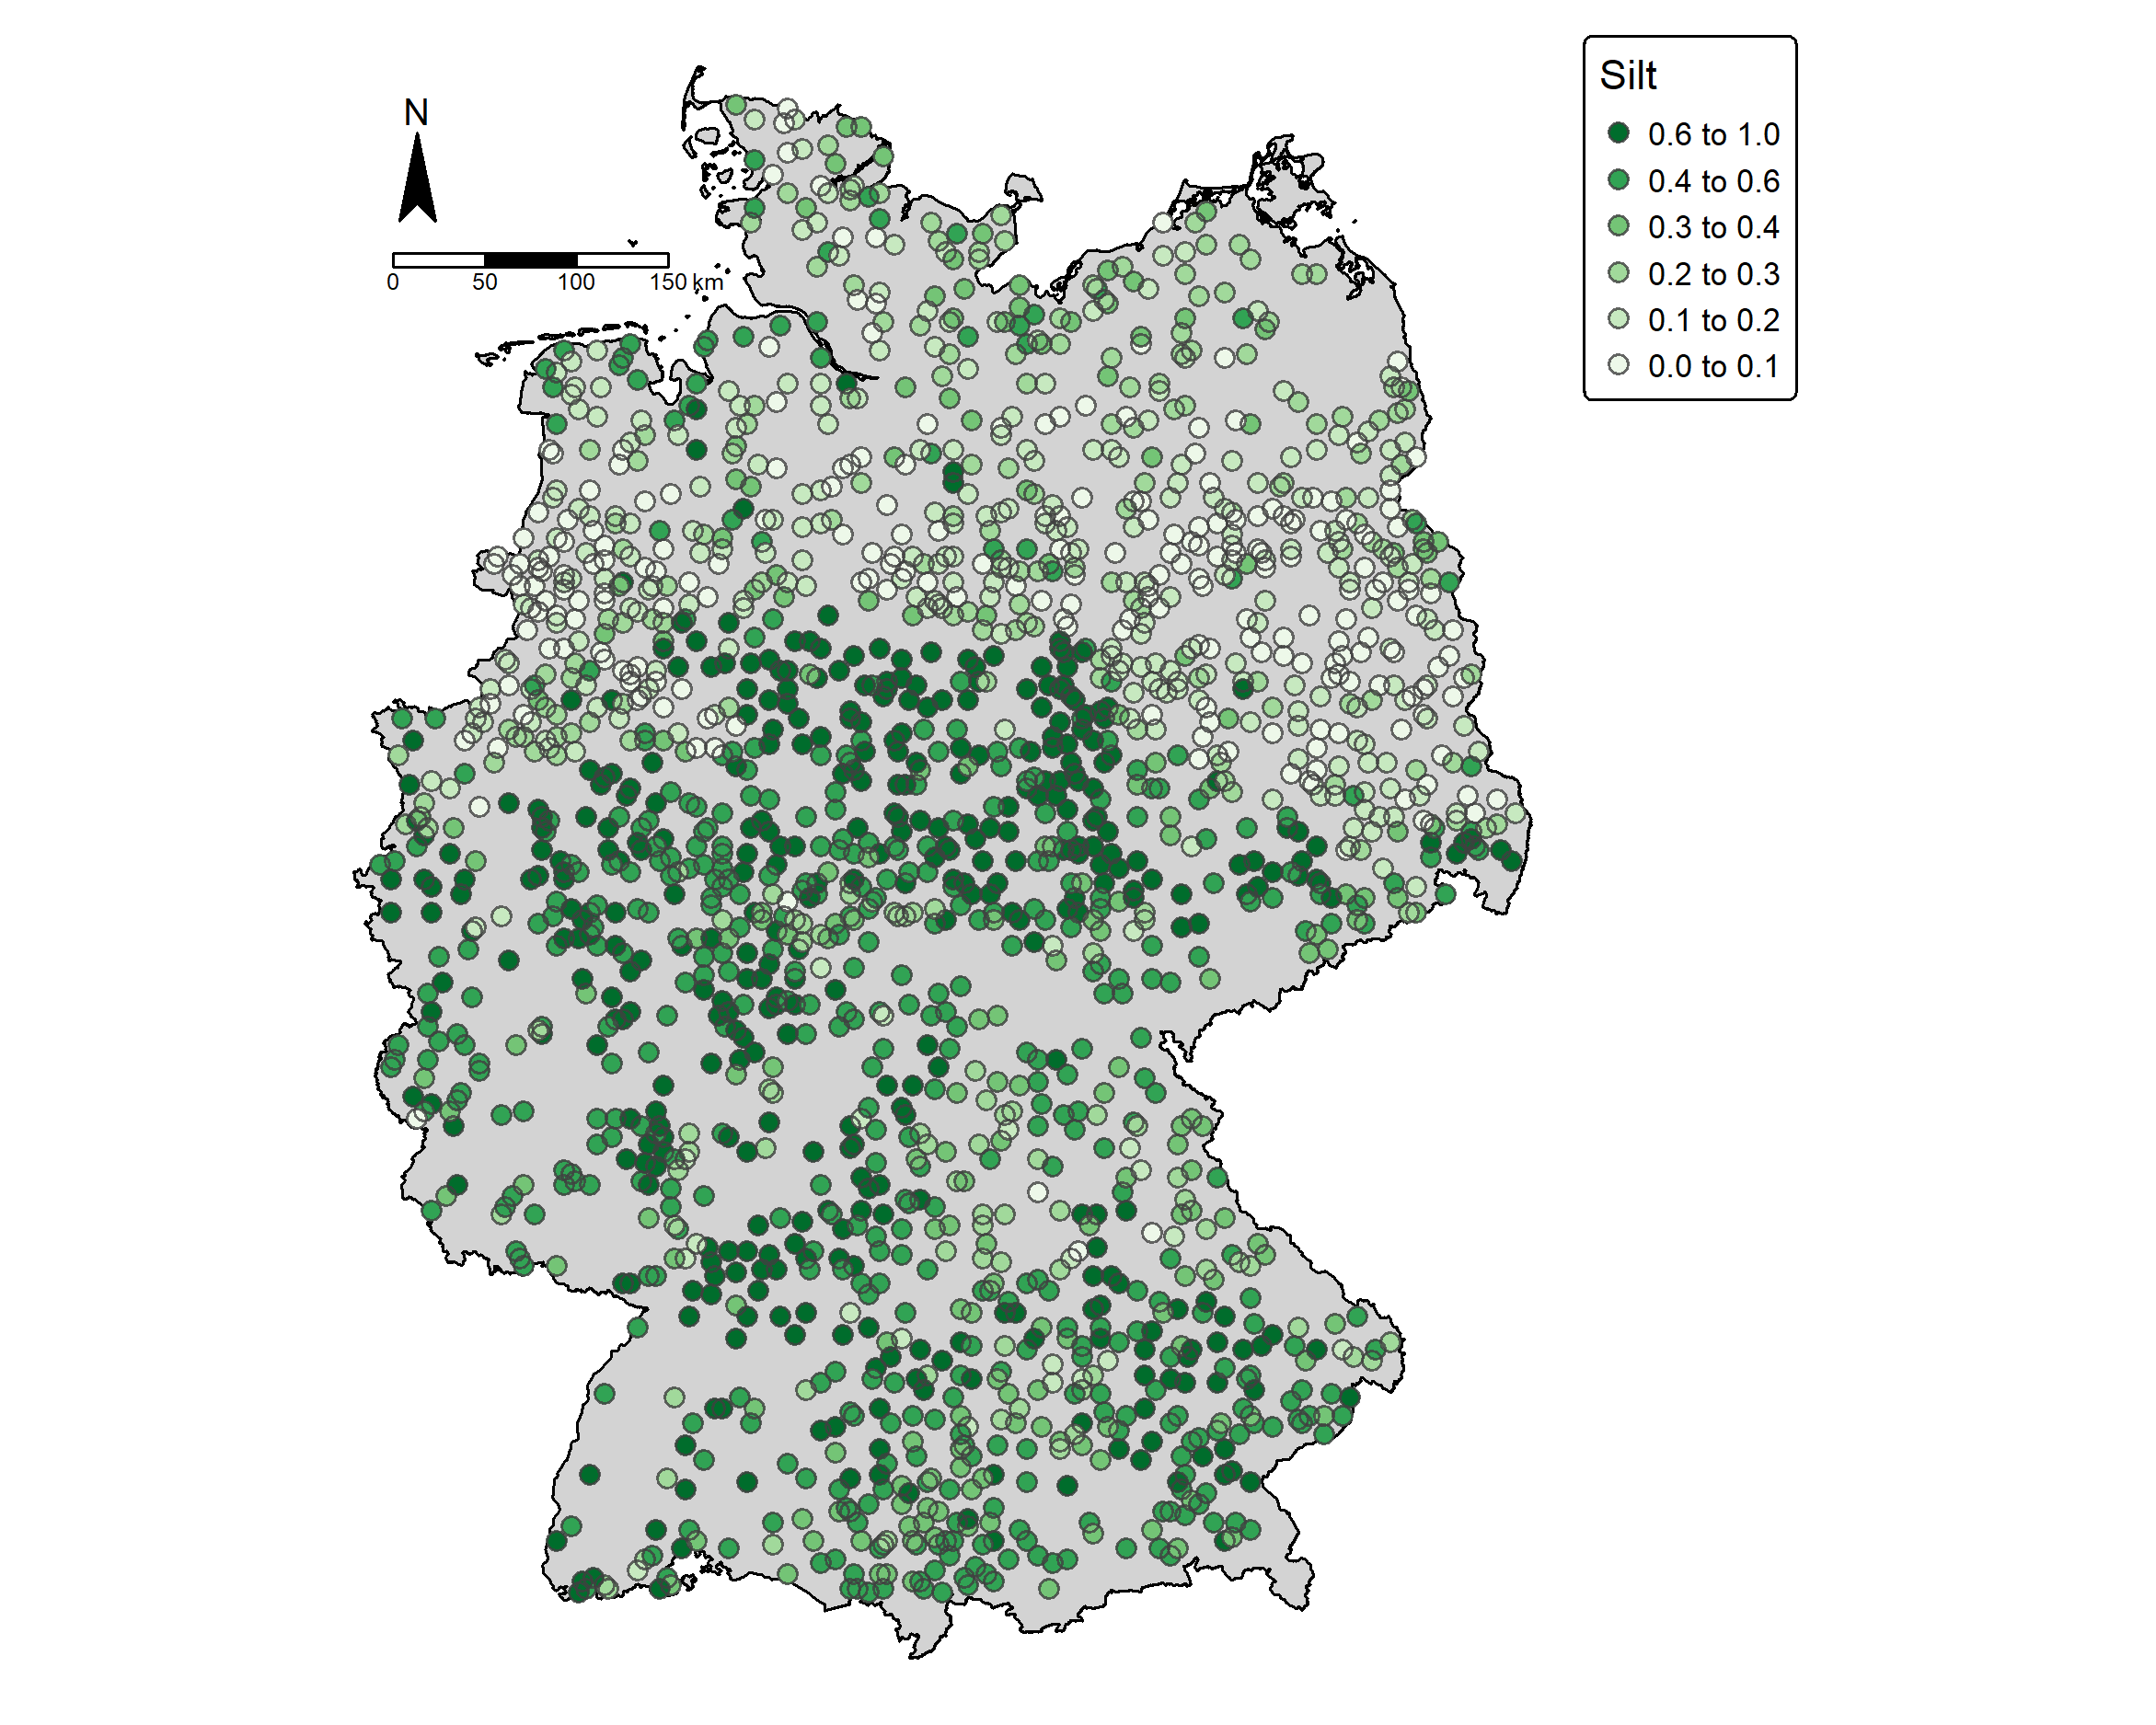
\includegraphics[width=\linewidth]{Figures/pointmap_silt.png}
            \caption{LUCAS soil texture observation locations in Germany: Silt.}
        \end{figure}}
    \end{column}

\end{columns}

\end{frame}

\begin{frame}{Ternary Plot of Soil Texture}

\begin{columns}

    \begin{column}{0.45\textwidth}
        \begin{itemize}
            \item[1.] A \textbf{ternary plot} is a triangle where each corner represents $100\%$ of one component: clay, sand, or silt.

           
            
            \item[2.] Points closer to a corner have a \textbf{higher proportion} of that component.

            \item[3.] Most observations cluster along the \textbf{sand--silt} edge, meaning few samples have high clay content.

            \item[4.] The spread of points reflects the \textbf{large variability} of sand and silt compared to clay.
        \end{itemize}
    \end{column}

    \begin{column}{0.55\textwidth}
        \begin{figure}
            \centering
            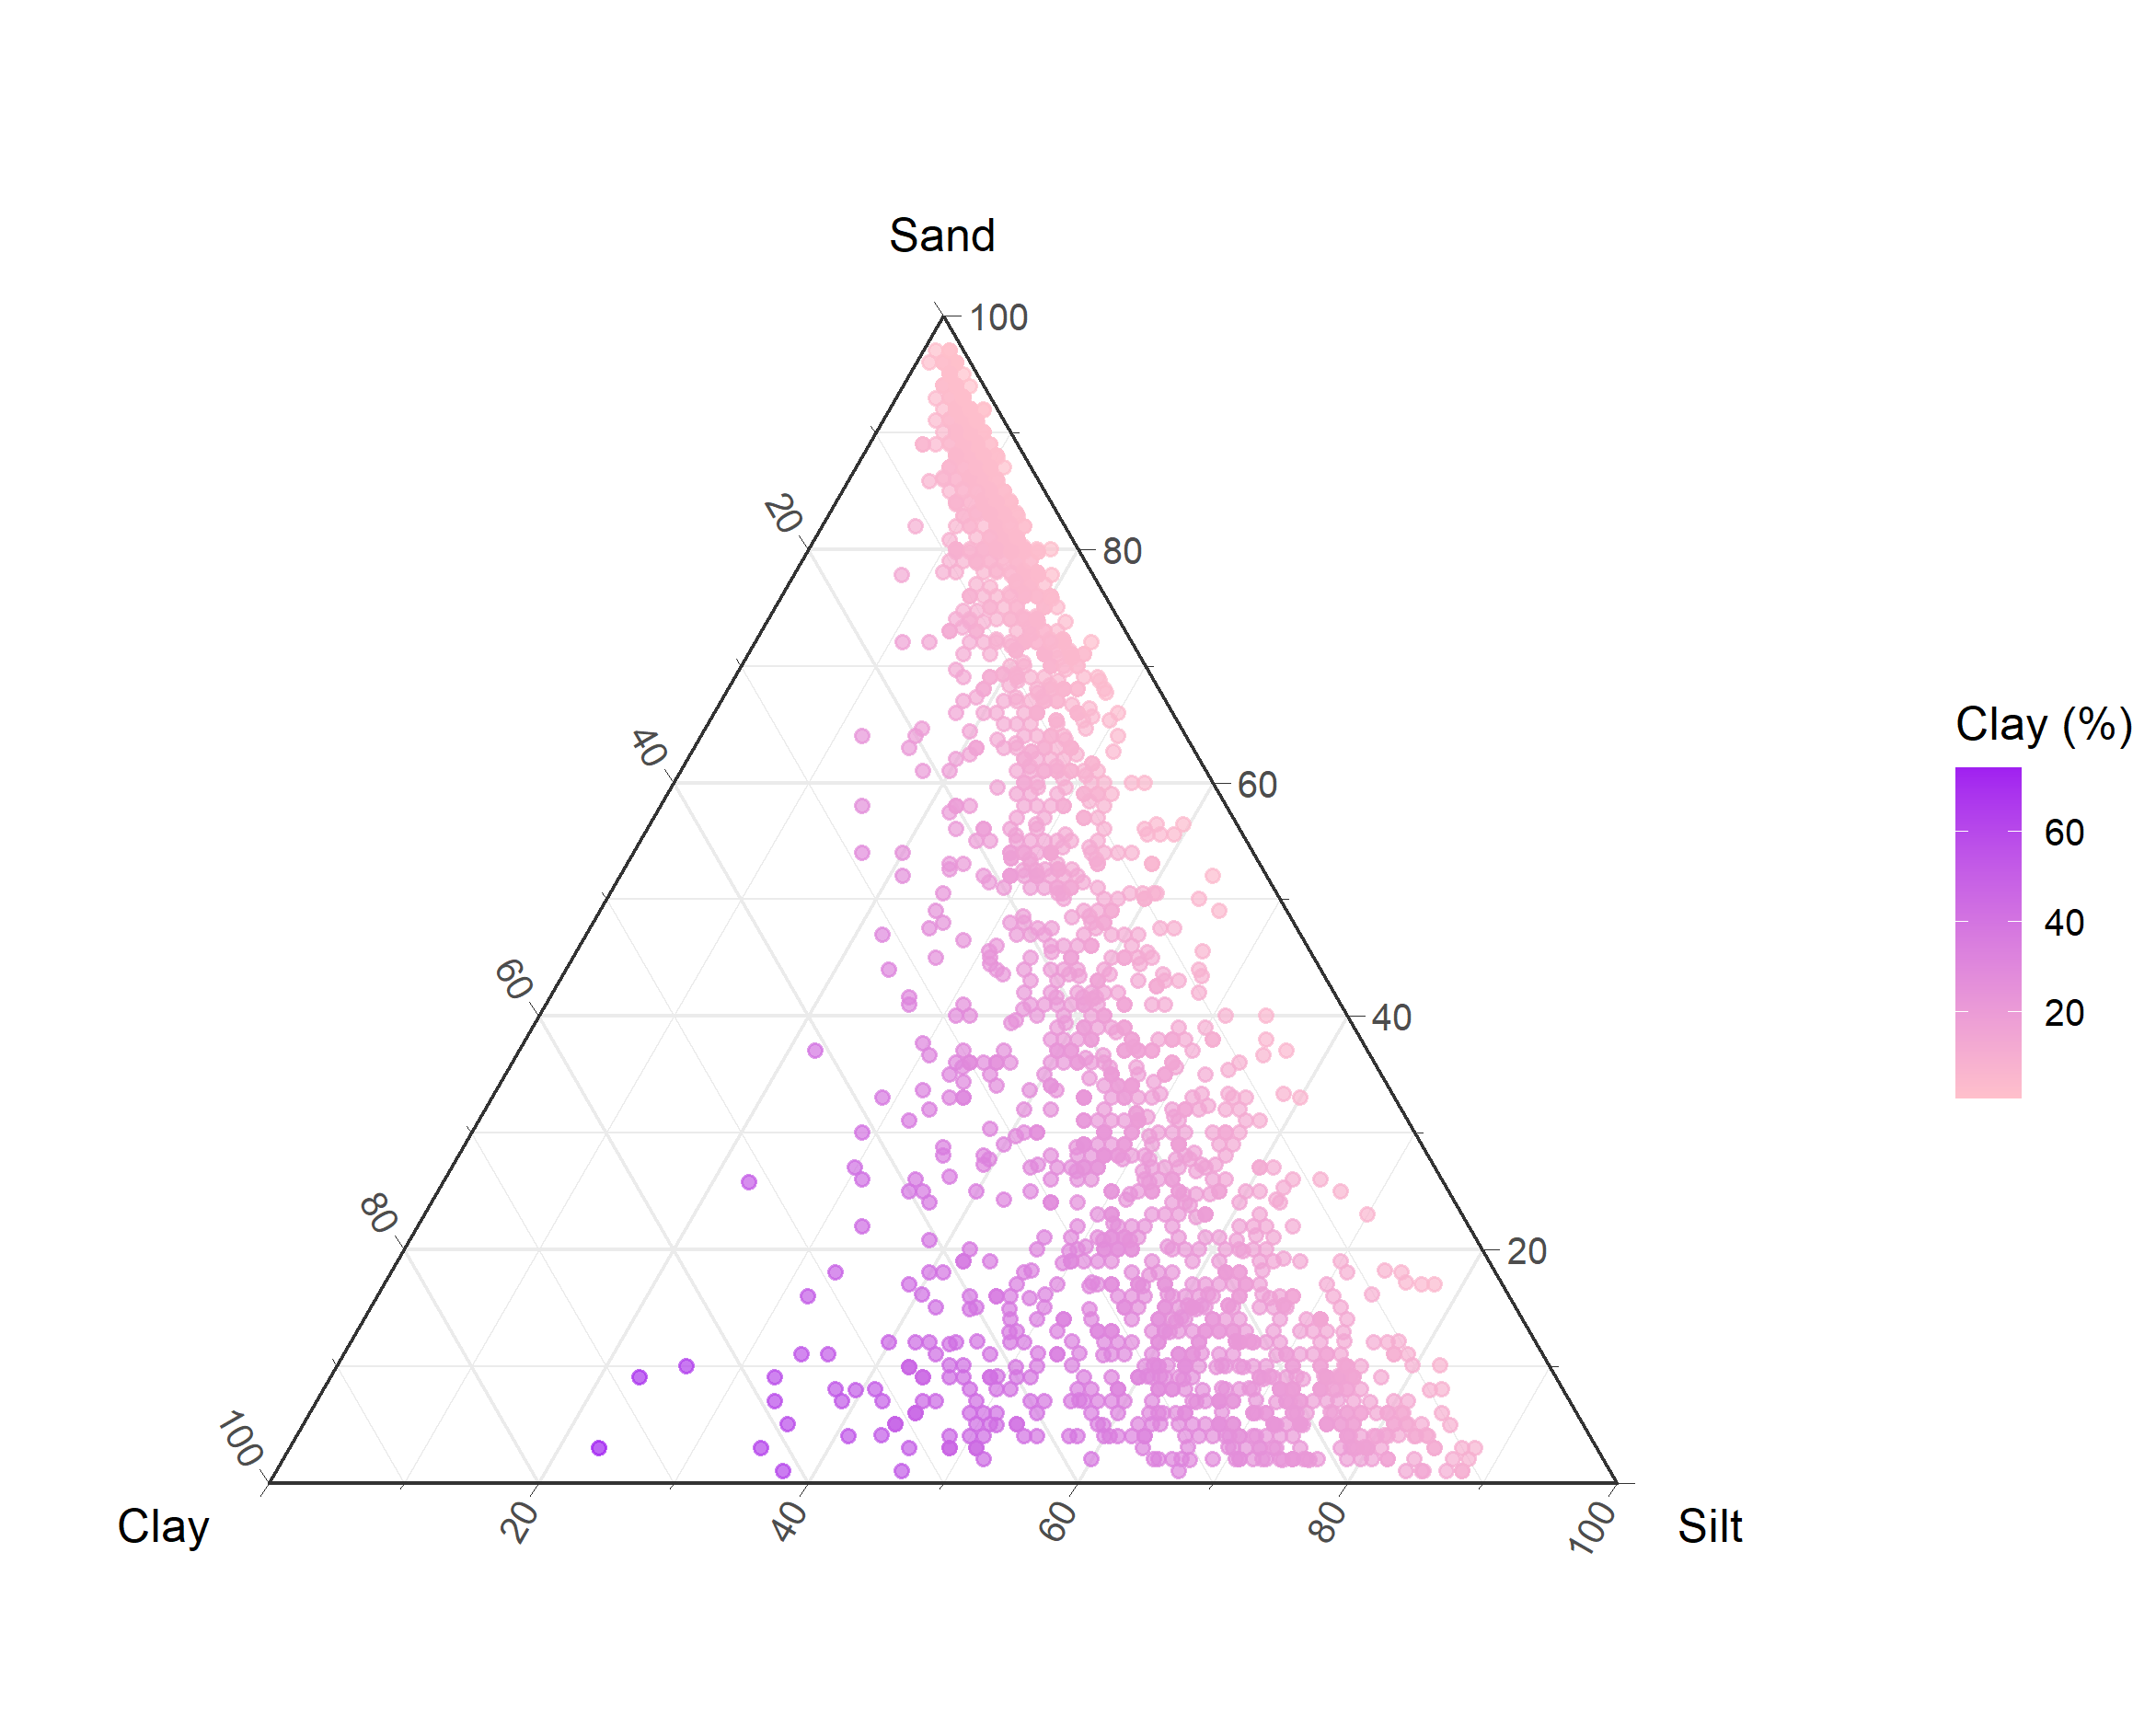
\includegraphics[width=\linewidth]{Figures/point_tern.png}
            \caption{Ternary plot of clay, sand, and silt distributions.}
        \end{figure}
    \end{column}

\end{columns}

\end{frame}

%% ─── SLIDE 4: Modelling Strategies ─────────────────────────────────────────
\begin{frame}{Modelling Strategies}

Five modelling approaches were compared:

\begin{table}
\centering
\small
\begin{tabular}{lccc}
\toprule
Model & Joint estimation & Respects geometry & Transformation \\
\midrule
RF (raw)         & No  & No  & No  \\
MRF (raw)        & Yes & No  & No  \\
ilr-RF           & No  & Yes & Yes \\
ilr-MRF          & Yes & Yes & Yes \\
\textbf{DirichletRF}   & Yes & Yes & No  \\
\bottomrule
\end{tabular}
\caption{Summary of modelling strategies.}
\end{table}

\begin{itemize}
    \item RF and MRF on raw components serve as \textbf{baseline} approaches.
    \item \textbf{DirichletRF} works directly on the simplex without requiring any log-ratio transformation.
\end{itemize}

\end{frame}




%% ─── SLIDE 4: Modelling Strategies ─────────────────────────────────────────
\begin{frame}{Evaluation Metrics}

To compare these models, we used  the Aitchison Distance and the Root Mean Square Error, or RMSE.
\vspace{0.2cm}
\textbf{1. Aitchison Distance:}
\[
AC = \frac{1}{n} \sum_{i=1}^n \sqrt{\sum_{j=1}^k \left(\log\frac{Y_{ij}}{g(\mathbf{Y}_i)} - \log\frac{\hat{Y}_{ij}}{g(\hat{\mathbf{Y}}_i)}\right)^2},
\]
\[
\text{where} \quad g(\mathbf{Y}_i) = \left(\prod_{j=1}^k Y_{ij}\right)^{1/k}
\]
\textit{Measures compositional dissimilarity using log-ratio geometry.}

\vspace{0.3cm}
\textbf{2. Root Mean Square Error (RMSE):}
$
\text{RMSE}_k =  \sqrt{\frac{1}{n} \sum_{i=1}^n (Y_{ij} - \hat{Y}_{ij})^2}
$

\vspace{0.3cm}
\textbf{Interpretation:} Lower values for both metrics indicate better predictive accuracy.
\end{frame}



\begin{frame}{Parameter Tuning and Cross-Validation}

\begin{itemize}
    \item[1.] All models were assessed using \textbf{10-fold nested cross-validation},
    with the same folds shared across methods to ensure a fair comparison.

    \item[2.]  Each random forest model was fitted with \textbf{500 trees}.

    \item[3.]  Hyper-parameters were selected by grid search:
    \begin{itemize}
        \item[3.1]  minimum node size: $\{2, 5, 10\}$
        \item[3.2] $m_{\mathrm{try}}$: $\{23, 29, 35, 41, 47, 53, 59, 65\}$
    \end{itemize}

    \item[4.] For \textbf{DirichletRF}, minimum node size was fixed at 5 for computational efficiency.

    \item[5.] Performance was quantified using \textbf{RMSE} and \textbf{Aitchison distance}.

    \item[6.] For the  comparison, models were refitted on the full dataset using
    the best hyper-parameters from the inner folds.
\end{itemize}

\end{frame}




%% ─── SLIDE 6: Results ───────────────────────────────────────────────────────
\begin{frame}{Results: RMSE and Aitchison Distance}

\begin{table}
\centering
\small
\caption{RMSE and Aitchison Distance (AC) across modelling approaches.}
\begin{tabular}{lccccc}
\toprule
 & RF & ilr-RF & MRF & ilr-MRF & \textbf{DirichletRF} \\
\midrule
\multicolumn{6}{c}{\textbf{RMSE}} \\
\midrule
Clay        & 0.086 & 0.086 & 0.088 & 0.087 & \textbf{0.085} \\
Sand        & 0.186 & 0.181 & 0.188 & 0.182 & \textbf{0.168} \\
Silt        & 0.148 & 0.145 & 0.150 & 0.146 & \textbf{0.135} \\
Aggregated  & 0.140 & 0.137 & 0.142 & 0.138 & \textbf{0.130} \\
\midrule
\multicolumn{6}{c}{\textbf{Aitchison Distance (AC)}} \\
\midrule
AC & 0.852 & 0.788 & 0.861 & 0.798 & \textbf{0.766} \\
\bottomrule
\end{tabular}
\end{table}

\begin{itemize}
    \item \textbf{DirichletRF} achieves the lowest RMSE across all components and the smallest AC.
    \item The largest gains are observed for \textbf{sand} and \textbf{silt}.
    \item ilr-based models only marginally outperform their untransformed counterparts.
\end{itemize}

\end{frame}


%% ─── FRAME 1: Cross-Validation Explanation ──────────────────────────────────
\begin{frame}{Publication}

\begin{center}
\vfill

\begin{block}{}
\begin{center}
\textbf{Dirichlet Random Forest for Predicting Compositional Data}\\[0.4em]
\end{center}
\end{block}

\vspace{0.5em}

\textbf{Authors:}\\[0.3em]
\underline{Masoumifard, K.}, van der Westhuizen, S., Gardner-Lubbe, S.

\vspace{0.8em}

\textbf{In:}\\[0.3em]
A. Bekker et al.\ (Eds.),\\
\textit{Environmental Modelling with Contemporary Statistics:\\
Learning, Directionality, and Space-Time Dynamics}\\[0.3em]
CRC Press\\[0.3em]
ISBN: 9781032903910

\vfill
\end{center}

\end{frame}
%\begin{frame}{Library on GitHub}
\only<1>{
\note{
For our DDRF method, we have developed an R library. It is available on CRAN and on GitHub. You can access it using this QR code.

}

  \begin{center}

    \qrcode{https://github.com/Xaleed/DirichletRF.git}
 \end{center}
    
    \centering
    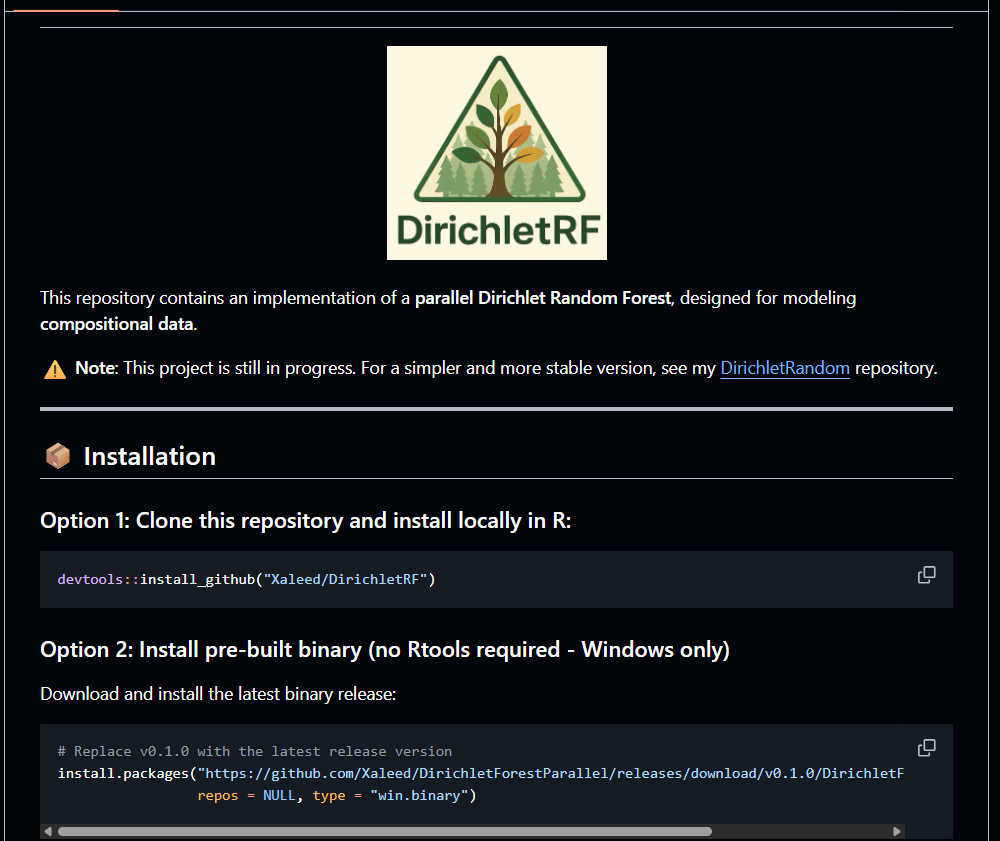
\includegraphics[width=0.45\linewidth]{slides/github.png}
    \caption{}
}
% \only<2>{
% \note{
% We developed an R library for this Random Forest model. This library implements the Random Forest in parallel and provides both predictions and empirical distributions. The parameters can be estimated using either Maximum Likelihood Estimation (MLE) or the Method of Moments (MoM), with MoM being the default option.

% }
%   \begin{center}

%     \qrcode{https://github.com/Xaleed/DirichletRF.git}
%  \end{center}
% %\vspace{0.3cm}

% \textbf{Key Features:}
% \begin{itemize}
% \item[\textcolor{blue}{\large$\blacktriangleright$}] Dirichlet distribution-based splits (likelihood maximization)
% \item[\textcolor{blue}{\large$\blacktriangleright$}] Parallel processing (Unix/Mac fork, Windows cluster)
% \item[\textcolor{blue}{\large$\blacktriangleright$}] Two purpose: Prediction vs. Distributional
% \item[\textcolor{blue}{\large$\blacktriangleright$}] Two parameter estimation methods (MoM, MLE)
% \end{itemize}


% }
    
\only<2>{
% \note{
% Most of the parameters are the same as in other well-known libraries. Here, we introduce two new parameters: \texttt{method} and \texttt{store\_samples}. I will briefly explain both.


% }
\begin{table}
\small
\begin{tabular}{lp{3cm}p{6cm}}
\toprule
\textbf{Parameter} & \textbf{Default} & \textbf{Description} \\
\midrule
\texttt{num.trees}  & 100          & Number of trees in the forest \\
\texttt{max.depth}  & 10           & Maximum tree depth \\
\texttt{min.node.size} & 5         & Minimum observations per leaf node \\
\texttt{mtry}       & $\sqrt{p}$   & Candidate features at each split \\
\texttt{seed}       & 123          & Random seed for the C++ RNG \\
\texttt{\textcolor{blue}{est.method}} & \texttt{"mom"} & Dirichlet estimation: \texttt{"mom"} or \texttt{"mle"} \\
\texttt{num.cores}  & $-1$         & OpenMP threads ($-1$ = all cores minus one) \\
\bottomrule
\end{tabular}
\end{table}
}
\end{frame}




% \begin{frame}{Conclusion}
%     \begin{itemize}

%     \item[\textcolor{blue}{\large$\blacktriangleright$}] 
%     \textbf{For compositional data}, we adapt Random Forest splitting rules to respect the geometry of the simplex, avoiding the limitations and potential bias introduced by traditional transformations to real space.
%     \vspace{1.1em}

%     \item[\textcolor{blue}{\large$\blacktriangleright$}] 
%     \textbf{Based on  comparison results, the model shows strong and stable performance}
%     across a wide range of scenarios.
%     \vspace{1.1em}

%     \item[\textcolor{blue}{\large$\blacktriangleright$}] 
%     \textbf{We also provide an open-source implementation} 
%     available as a Git/R package.
% \end{itemize}
% \end{frame}



%
\begin{frame}
 
\frametitle{\resizebox{.95\linewidth}{!}{%
Addressing Dirichlet's Limitations: Extensions \& Alternatives}}
\note{Now, I want to talk about three useful versions of the Dirichlet distribution:

First, the Zero-Inflated Dirichlet. This model is good when we have many zeros in the data. The standard Dirichlet cannot handle zeros well, but this one can.

Second, the Nested Dirichlet. The standard Dirichlet assumes all parts are negatively related. This is not always true in real data. The nested version helps fix that.

Third, the Kummer–Dirichlet. This model is better when the data has outliers. It is more flexible and gives more stable results.}
\begin{itemize}
  \item[\textcolor{blue}{\large$\blacktriangleright$}] \textbf{ Zero-Inflated Dirichlet Models:}  
  Handle compositional data with many zeros.

  \item[\textcolor{blue}{\large$\blacktriangleright$}] \textbf{ Nested–Dirichlet Models:}  
  Address the limitation of standard Dirichlet where all components are negatively correlated.

  \item[\textcolor{blue}{\large$\blacktriangleright$}] \textbf{Kummer–Dirichlet Models:}  
  Offer greater robustness to outliers compared to the standard Dirichlet.
\end{itemize}


\end{frame}

\begin{frame}
\frametitle{Distributional Dirichlet Random Forests (DRF)}
\note{
Another idea that I really like is to fit an empirical probability function.

Actually, we can fit a probability function on the training dataset. Then, for a new observation, we can evaluate this probability function to obtain its predicted distribution.

Actually, we can fit a probability function on the training dataset. This method was introduced in 2022. I will not go into the details of how it works. I have a simple example to explain it, but I will skip it to save time.
}

\begin{equation*}
P(Y = y_i \mid X = \mathbf{x}_{\text{new}}) = w_i(\mathbf{x}_{\text{new}}), \quad i = 1, \dots, n, \quad \sum_{i=1}^{n} w_i(\mathbf{x}_{\text{new}}) = 1.
\end{equation*}

\vspace{0.5em}
\begin{block}{}
The formula for the normalized weight $w_i$ is:
\[
w_i(\mathbf{x}_{\text{new}})
= \frac{1}{B} \sum_{k=1}^B 
\frac{\mathbf{1}\!\left(\mathbf{x}_{\text{new}} \in L_k(i)\right)}{|L_k(i)|}.
\]
where $|L_k(i)|$ is the size of the terminal node in tree $k$ where $\mathbf{x}_{\text{new}}$ falls.
\end{block}
\end{frame}



\begin{frame}[plain]
  \begin{center}
    \vspace{2cm}

    {\Huge \textbf{Thank You!}\par}

    \vspace{1cm}

    
\includegraphics[width=0.15\linewidth]{slides/DirichletRF.jpg}

    %\vspace{0.8cm}

    % QR code (requires: \usepackage{qrcode})
    \qrcode[height=1.8cm]{https://github.com/Xaleed/DirichletRF.git}

    \vspace{0.1cm}

    {\small QR code for the GitHub repository}

  \end{center}
\end{frame}


%


\begin{frame}{Why Ambiguous!}
   \only<1>{

   \frametitle{Principles of CODA}
      \begin{itemize}
       \item 
   \textbf{scale invariance},
   \item
   \textbf{permutation invariance}, and 
   \item \textbf{subcompositional coherence}
   If \( \Delta_p(\mathbf{x}, \mathbf{y}) \) denotes a distance measure between compositions with \( p \) parts, then
    \begin{equation*}
    \Delta_k(\mathbf{x}, \mathbf{y}) \geq \Delta_d(\mathbf{x}_d, \mathbf{y}_d),
    \end{equation*}
    where \( \mathbf{x}, \mathbf{y} \) are compositions with \( k \) parts, and \( \mathbf{x}_d, \mathbf{y}_d \) are corresponding subcompositions with \( d < k \) parts.
    \end{itemize}}
\only<2>{
\textbf{\textcolor{blue}{Question 1:}} Are these principles designed to achieve consistent results with the original data $\mathbf{Y}$?  

The arguments supporting $\mathbf{a}(\mathbf{Y})$ are rarely evaluated for consistency with the original vector $\mathbf{Y}$, even though Aitchison himself criticized standard statistical approaches for inconsistency with the original data.
}

\only<3>{
As an illustration, consider
\[
\mathbf{S}(\mathbf{Y}) = \Big( \frac{Y_1}{Y_1 + Y_2}, \frac{Y_2}{Y_1 + Y_2} \Big) = (U, 1-U).
\]
\textbf{\textcolor{blue}{Can we assume that \(U\) follows a Beta distribution?}}

\textbf{\textcolor{red}{Aitchison's critique:}} For \(U\) to follow a Beta distribution,
\[
Y_i \sim^{\text{iid}} \text{Gamma}(\alpha_i, \lambda), \quad i=1,2.
\]
This generalizes naturally to the Dirichlet distribution.

His proposal instead:
\[
\left(\frac{1}{2}\ln\frac{Y_1}{Y_2}, \frac{1}{2}\ln\frac{Y_2}{Y_1}\right)
\]
}

\only<4>{
\textbf{\textcolor{blue}{Question 2:}} Are these principles designed to provide non-spurious correlations?

Correlations among components of $\mathbf{a}(\mathbf{Y})$ are themselves spurious.
}

\only<5>{
\textbf{Spurious correlation example:}

Even if  
\[
\operatorname{corr}(Y_1, Y_2)=0,
\]
we usually observe
\[
\boxed{
\operatorname{corr}\Big(\frac{Y_1}{S}, \frac{Y_2}{S}\Big) \neq 0, \quad S=\sum_{j=1}^{D} Y_j
}
\]
\textbf{Reason:} shared denominator induces dependency.
}

\only<6>{
\[
\boxed{
\operatorname{corr}\Big(\frac{Y_1}{S}, \frac{Y_2}{S}\Big)
=
\frac{
\mathbb{E}\Big(\frac{Y_1 Y_2}{S^2}\Big) - \mathbb{E}\Big(\frac{Y_1}{S}\Big)\mathbb{E}\Big(\frac{Y_2}{S}\Big)
}{
\sqrt{\operatorname{Var}\Big(\frac{Y_1}{S}\Big)} \sqrt{\operatorname{Var}\Big(\frac{Y_2}{S}\Big)}
}
}
\]

\textbf{Key point:} The formula is mathematically valid; the issue is interpretation:
\[
\operatorname{corr}\Big(\frac{Y_1}{S}, \frac{Y_2}{S}\Big) \not\Rightarrow \operatorname{corr}(Y_1,Y_2)
\]
}

\only<7>{
\textbf{Frequently emphasized in CODA:}

\begin{block}{Different denominators}
\[
\left(\frac{Y_1}{S_4},\frac{Y_2}{S_4},\frac{Y_3}{S_4},\frac{Y_4}{S_4}\right),\quad
\left(\frac{Y_1}{S_3},\frac{Y_2}{S_3},\frac{Y_3}{S_3}\right)
\]
\end{block}

\begin{alertblock}{Claimed problem}
\[
\operatorname{corr}\Big(\frac{Y_1}{S_4}, \frac{Y_2}{S_4}\Big) \neq \operatorname{corr}\Big(\frac{Y_1}{S_3}, \frac{Y_2}{S_3}\Big)
\]

\textbf{Both correlations are spurious.}  
It is unclear why equality between two spurious correlations should matter.
\end{alertblock}
}

\only<8>{
\begin{block}{ILR (or Other) Transformed Coordinates}

\begin{minipage}{0.48\textwidth}
\centering
\textbf{} \\[2mm]
\scalebox{0.75}{$
\mathbf{T}_4 = T\Big(\frac{Y_1}{S_4},\frac{Y_2}{S_4},\frac{Y_3}{S_4},\frac{Y_4}{S_4}\Big):(T_1,T_2,T_3,T_4)
$} \\[2mm]
\scalebox{0.75}{$
\mathbf{T}_3 = T\Big(\frac{Y_1}{S_4},\frac{Y_2}{S_4},\frac{Y_3}{S_4}\Big):(T_1,T_2,T_3)
$}
\end{minipage}
\hfill
\begin{minipage}{0.48\textwidth}
\centering
\textbf{} \\[2mm]
\scalebox{0.75}{$
\mathbf{T}'_4 = T\Big(\frac{Y'_1}{S'_4},\frac{Y'_2}{S'_4},\frac{Y'_3}{S'_4},\frac{Y'_4}{S'_4}\Big):(T'_1,T'_2,T'_3,T'_4)
$} \\[2mm]
\scalebox{0.75}{$
\mathbf{T}'_3 = T\Big(\frac{Y'_1}{S'_4},\frac{Y'_2}{S'_4},\frac{Y'_3}{S'_4}\Big):(T'_1,T'_2,T'_3)
$}
\end{minipage}

\end{block}


\begin{alertblock}{Subcompositional Coherence}
\scalebox{0.85}{\[
D_3(\mathbf{T}_3,\mathbf{T}'_3) \le D_4(\mathbf{T}_4,\mathbf{T}'_4)
\]}
\begin{center}
\textbf{\large Surprisingly, the correlations between components remain \textcolor{red}{spurious}, 
but we cannot work in the simplex space accordingly.}
\end{center}
\end{alertblock}
}

\only<9>{
\textbf{\textcolor{blue}{Question 2:}} Are these principles designed to provide non-spurious correlations?  The answer is no.
}

\only<10>{
\textbf{\textcolor{blue}{Question 3:}} Are these principles designed to satisfy theoretical requirements?

It is important to note that \(\mathbf{s}(\cdot)\)  is subset of real space and therefore inherit its standard geometric structure, rendering all conventional mathematical operations well-defined.
}

\only<11>{
\textbf{\textcolor{blue}{Question 4:}} Are these principles widely accepted?  The answer is no.
}

\end{frame}



\begin{frame}{Critics of CoDA: Early and Ongoing}
A number of authors have questioned the strict log-ratio framework
promoted by the “CoDa School.” Major groups include:
\scriptsize   % shrinks everything but remains readable


\begin{itemize}\itemsep1pt
    \item \textbf{Watson}: objections to distance measures and geometry
    \item \textbf{Zier \& Rehder}: challenges to mathematical definitions
    \item \textbf{Butler \& Glasbey}: alternative approaches for zeros
    \item \textbf{Stewart \& Field}: practical issues in real applications
    \item \textbf{Tsagris et al.}: limits for highly variable data
    \item \textbf{Scealy \& Welsh}: critique of the Principles themselves
\end{itemize}



\end{frame}




\begin{frame}{Key Critics: D.F. Watson}
\scriptsize   % shrinks everything but remains readable

    \begin{itemize}
        \item \textbf{D.F. Watson} was a central figure in early debates against Aitchison's log-ratio methods.
        \item **Main Criticism Focus:**
        \begin{itemize}
            \item Questioned the fundamental need for "scale invariance," a core principle of the CoDa School.
            \item His exchanges with Aitchison in \textit{Mathematical Geology} (1989-1992) were instrumental in the development of the CoDa Principles, though from a critical stance.
            \item The text notes that "Watson \& Philip (1989) ... did not see the need for scale invariance."
        \end{itemize}
        \item Tragically, his contributions were cut short due to a contentious exchange where Aitchison used derogatory language.
    \end{itemize}
\end{frame}
\begin{frame}{Key Critics: Zier \& Rehder}
\scriptsize   % shrinks everything but remains readable

    \begin{itemize}
        \item \textbf{Zier \& Rehder} (1998, 2001) continued to raise points against the CoDa School's established views.
        \item **Main Criticism Focus:**
        \begin{itemize}
            \item Challenged technical issues, particularly related to the mathematical definition of a metric within compositional data analysis.
            \item Like Watson, they "did not see the need for scale invariance," arguing it problematic if compositions are strictly defined as summing to one.
            \item Their arguments highlighted that even Aitchison's own earlier work might not have strictly adhered to the current CoDa definition of compositions and scale invariance.
        \end{itemize}
        \item Despite making "some good points," their criticisms were "dismissed relatively easily" by the CoDa School, partly due to perceived technical mistakes on their part.
    \end{itemize}
\end{frame}
\begin{frame}{Key Critics: Butler \& Glasbey}
\scriptsize   % shrinks everything but remains readable

    \begin{itemize}
        \item \textbf{Butler \& Glasbey} (2008) represent a more recent wave of critics whose methods were deemed "unapproved" by the CoDa School.
        \item **Main Criticism Focus:**
        \begin{itemize}
            \item Developed "otherwise sensible analysis" methods that did not conform to the CoDa Principles.
            \item Were compelled to "list and explain their 'failings' relative to the Principles."
            \item Their work highlighted that theoretical difficulties with the Principles meant their methods could only be used as "diagnostic tool or for exploratory analysis" according to CoDa proponents.
            \item This illustrates how the Principles act as a barrier to new methodological developments.
        \end{itemize}
    \end{itemize}
\end{frame}
\begin{frame}{Key Critics: Stewart \& Field, Tsagris et al., Scealy \& Welsh}
\scriptsize   % shrinks everything but remains readable

    \begin{itemize}
        \item \textbf{Stewart \& Field (2010), Tsagris, Preston \& Wood (2011), and Scealy \& Welsh (2011a, 2011b)} also demonstrate the practical limitations of the CoDa School's exclusive approach.
        \item **Main Criticism Focus:**
        \begin{itemize}
            \item Provided "interesting real examples where important practical differences produced by a variety of methods are highlighted."
            \item Showed that the differences between various methods become particularly important for \textbf{highly variable data near or on the boundary of the simplex}.
            \item \textbf{Scealy & Welsh (2011a, 2014, the source text)} specifically critique the **motivation, justification, and relevance of the Principles themselves**, particularly subcompositional coherence.
            \item They argue against the logical basis for scale invariance and subcompositional dominance, proposing alternatives like "amalgamations" as more suitable 'marginals'.
        \end{itemize}
    \end{itemize}
\end{frame}
\begin{frame}{Conclusion on Criticisms}
\scriptsize   % shrinks everything but remains readable

    \begin{itemize}
        \item These critics collectively highlight significant issues:
        \begin{itemize}
            \item The contested definition of a "composition."
            \item The rigid and sometimes illogical foundations of the CoDa Principles (e.g., scale invariance, subcompositional coherence).
            \item The active dismissal of valid alternative methods simply for not conforming to these Principles.
            \item The practical limitations of the CoDa approach, especially with challenging data.
        \end{itemize}
        \item The text emphasizes that the existence and application of these Principles in such a restrictive way is "unusual, perhaps even unique, in statistical data analysis."
    \end{itemize}
\end{frame}



\begin{frame}{The Aitchison-Watson Debate: A Contentious Beginning}
\scriptsize   % shrinks everything but remains readable

    \begin{itemize}
        \item The foundational "Principles of Compositional Data Analysis" largely evolved from a series of intense exchanges.
        \item Primarily, this involved papers and letters between \textbf{J. Aitchison} (as the defender/proponent of log-ratio methods) and \textbf{D.F. Watson} (as a critic of the nascent CoDa School's approach).
        \item These debates, published in \textit{Mathematical Geology} from 1989-1992, set the stage for much of the field's development and controversies.
        \item However, the intellectual exchange took a negative turn:
        \begin{itemize}
            \item Aitchison is noted to have used the word "stupid" in reference to Watson's arguments.
            \item This pejorative remark led to \textbf{Watson discontinuing his contributions} to the debate, effectively silencing a critical voice.
        \end{itemize}
        \item This event highlights how personal attacks can impede scientific discourse and shape the trajectory of a research field.
        \item Scealy & Welsh (2014) emphasize that "the exchange between Watson and Aitchison had a negative impact on both sides and contributed directly to the situation in modelling and analysing compositional data that we have today."
    \end{itemize}
\end{frame}


%\begin{frame}{Simplex space}
\only<1>{
\note{
In this presentation, I will frequently refer to simplex space. 
A simplex space is collection of vectors with non-negative values that always sum to a constant.
This space is known as the \emph{simplex} and it is common to set \( k = 1 \).
We refer to data from this space as \emph{compositional data}.
}

\vspace{1em}

A simplex is a convex space of all vectors with non-negative components that sum to a constant. 

\begin{center}
\colorbox{blue!10}{\parbox{0.8\textwidth}{
\begin{center}
\[
S^c_k = \left\{ (y_1, \dots, y_k)^\top \in \mathbb{R}^k \,\middle|\, y_i \geq 0, \ \sum_{i=1}^k y_i = \textcolor{blue}{c} \right\}
\]
\end{center}
}}
\end{center}

It is common to set \(  \textcolor{blue}{c = 1} \). We refer to data from this space as \emph{compositional data}.
}

\only<2>{
\note{Another important space in the context of compositional data is the Aitchison space. This space is a log-transformed version of the simplex. Another important log-ratio transformation is the isometric log-ratio (ILR) transformation.
In reality, there is a wide variety of log-ratio transformations of the simplex space. }
Aitchison space:
\begin{center}
\colorbox{blue!10}{\parbox{1\textwidth}{
\begin{center}
\[
A_k = \left\{\left(\ln\!\left(\frac{Y_1}{g(\mathbf{Y})}\right), \ldots, \ln\!\left(\frac{Y_{k}}{g(\mathbf{Y})}\right)\right); g(\mathbf{Y}) = \left(\prod_{i=1}^{k} Y_i\right)^{1/{k}}\right\}
\]
\end{center}
}}
\end{center}
}
\end{frame}


\begin{frame}{Compositional data}
\only<1>{
\note{
Consider a vector with \(K\) components, where the only constraint is that all components are non-negative. Two important transformations of this vector are the following vectors. 

1. transform data to simplex space

2. transform data to Aitchison space

so we have original vector, simplex vector and Aitchison vector.

In general, the original vector \(\mathbf{Y} = (Y_1, \ldots, Y_K) \in \mathbb{R}_+^K\) cannot be recovered from these transformations, because they remove information about the absolute scale of the components. However, the simplex representation and the Aitchison representation can be recovered from one another.

There are some challenges in interpreting results that are based on the Simplex or Aitchison space.
}

Consider a vector \(\mathbf{Y} = (Y_1, Y_2, \ldots, Y_k) \in \mathbb{R}_+^k\). Two commonly used transformations of \(\mathbf{Y}\) are of particular interest:  

\begin{equation*}
\mathbf{S}_{k}(\mathbf{Y}) = \left(\frac{Y_1}{\sum_{i=1}^{k} Y_i}, \ldots, \frac{Y_{k}}{\sum_{i=1}^{k} Y_i}\right),
\end{equation*}

and  

\begin{equation*}
\mathbf{A}_{k}(\mathbf{Y}) = \left(\ln\!\left(\frac{Y_1}{g(\mathbf{Y})}\right), \ldots, \ln\!\left(\frac{Y_{k}}{g(\mathbf{Y})}\right)\right),
\end{equation*}

where \(g(\mathbf{Y}) = \left(\prod_{i=1}^{k} Y_i\right)^{1/{k}}\) denotes the geometric mean of \(\mathbf{Y}\). 
}

\only<2>{
\note{
it is simplest case of these two spaces.
}
Consider a vector \(\mathbf{Y} = (Y_1, Y_2) \in \mathbb{R}_+^2\). 

\begin{equation*}
\mathbf{S}(\mathbf{Y}) = \left(\frac{Y_1}{Y_1+Y_2},  \frac{Y_2}{Y_1+Y_2}\right),
\end{equation*}

and  

\begin{equation*}
\mathbf{A}(\mathbf{Y}) = \left(\frac{1}{2}\ln\!\left(\frac{Y_1}{Y_2}\right), \frac{1}{2}\ln\!\left(\frac{Y_2}{Y_1}\right)\right),
\end{equation*}

where \(g(\mathbf{Y}) = \left(\prod_{i=1}^2 Y_i\right)^{1/2}\) denotes the geometric mean of \(\mathbf{Y}\). 
}

\only<3>{
\note{
One important point is that the correlation between components 1 and 2 is \(-1\) in both the simplex and the Aitchison space, no matter what the correlation between \(Y_1\) and \(Y_2\) is.

this type correlation between components in the simplex or in the Aitchison space should \textbf{not} be interpreted as the correlation between the original components of \(\mathbf{Y}\). 

This is also true for higher dimensions. The correlations in these spaces can be far from zero, even when the true correlation between \(Y_1\) and \(Y_2\) is zero.
}

\textbf{Spurious correlations:} Based on Pearson (1897), correlations between the components of $\mathbf{S}(\mathbf{Y})$ or $\mathbf{A}(\mathbf{Y})$ should \textbf{not} be interpreted as correlations between the components of $\mathbf{Y}$.  

For example, 
\[
\boxed{
\begin{aligned}
&\text{cor}\left(\frac{Y_1}{Y_1 + Y_2}, \frac{Y_2}{Y_1 + Y_2}\right) = -1 \\[1em]
&\text{cor}\left(\frac{1}{2}\ln\left(\frac{Y_1}{Y_2}\right), \frac{1}{2}\ln\left(\frac{Y_2}{Y_1}\right)\right) = -1
\end{aligned}
}
\quad \Longrightarrow \quad \text{cor}(Y_1, Y_2) = 0
\]
}

\only<4>{
\note{
Pearson (1897) referred to this as \textit{spurious correlations}. His work marks the starting point of a long and ongoing effort to answer the following challenging question:

Which of the two transformations, simplex or Aitchison, provides the most desirable properties for statistical analysis and modeling?

After Pearson, many researchers argued that these spurious correlations happen because Euclidean metrics are not appropriate for the simplex. Surprisingly, they only refer to the simplex space, not the Aitchison space. But in both spaces the correlations are still spurious.
}

\textbf{Spurious correlations:}
\[
\boxed{
\begin{aligned}
&\text{cor}\left(\frac{Y_1}{\sum_{i=1}^{K} Y_i}, \frac{Y_2}{\sum_{i=1}^{K} Y_i}\right) \neq 0 \\[1em]
&\text{cor}\left(\frac{Y_1}{g(\mathbf{Y})}, \frac{Y_2}{g(\mathbf{Y})}\right) \neq 0
\end{aligned}
}
\quad \Longrightarrow \quad \text{cor}(Y_1, Y_2) = 0
\]

\textbf{\textcolor{blue}{Question}}: Which of the two transformations, \(\mathbf{s}(\mathbf{Y})\) or \(\mathbf{a}(\mathbf{Y})\), offers the most desirable properties for statistical analysis and modeling?
}

\only<5>{
\note{
I want to emphasize that the claim that ``Euclidean metrics are the problem'' is not correct. There is no mathematical problem that needs to be fixed. These spurious correlations are actually expected and understandable. We just need to be careful with how we interpret them.

This controversy and misunderstandings has had a negative effect on the proper development of methods for compositional data. As a result, the methodology for working directly in the simplex space has not been well explored.

However as we worked through literature we became convinced to focus on working directly in the simplex space, especially from a machine learning point of view.
}

\colorbox{green!10}{\parbox{0.95\textwidth}{
\[
\begin{aligned}
\operatorname{cor}\!\left(\frac{Y_1}{Y_1 + Y_2}, \frac{Y_2}{Y_1 + Y_2}\right)
=&
\operatorname{cor}\!\left(\frac{Y_1}{Y_1 + Y_2}, 1 - \frac{Y_1}{Y_1 + Y_2}\right)\\
= &
\operatorname{cor}\!\left(f(Y_1, Y_2),\, 1 - f(Y_1, Y_2)\right)
= -1.
\end{aligned}
\]
}}
}
\end{frame}


\begin{frame}{}
\only<1>{ 
\note{I want to quickly talk about the advantages of these two spaces.}

\textbf{\textcolor{blue}{Question}}: Which of the two transformations, \(\mathbf{s}(\mathbf{Y})\) or \(\mathbf{a}(\mathbf{Y})\), offers more desirable properties for statistical analysis and modeling.
}

\only<2>{ 
\note{One obvious advantage of the simplex space is that we can easily understand what each component represents. For example, suppose a class has 50 Mathematics, 100 Statistics, and 150 Computer Science students. In the simplex space, we can immediately say that, for instance, \(0.17\) of the students are from the Mathematics department.

In contrast, an Aitchison-transformed vector might give a value such as \(-0.6\), which has no direct, intuitive interpretation. To understand the meaning of such numbers, we must transform the vector back to the simplex space. Only then can the components be interpreted in terms of proportions or relative contributions.
}

\textbf{\textcolor{blue}{Advantage of \(\mathbf{s}(\mathbf{Y})\):}}

The advantage of $\mathbf{s}(\mathbf{Y})$ is its interpretability.

Example, consider 
\(
\mathbf{Y} = (50, 150, 100),
\)
represents the number of students in mathematics, statistics, and computer science in a class.  

Then
\begin{align*}
\mathbf{s}(\mathbf{Y}) 
&=\scalebox{1.2}{$\left(\frac{50}{50+150+100},\;\frac{150}{50+150+100},\;\frac{100}{50+150+100}\right)$} \\
&= (0.17, 0.50, 0.33), \\[6pt]
\mathbf{a}(\mathbf{Y})
&= \scalebox{1.1}{$\left(
\ln \frac{50}{(50 \times 150 \times 100)^{1/3}},\;\ 
\ln \frac{150}{(50 \times 150 \times 100)^{1/3}},\;\ 
\ln \frac{100}{(50 \times 150 \times 100)^{1/3}}
\right)$} \\
&= (-0.60, 0.50, 0.10).
\end{align*}

However, the components of $\mathbf{a}(\mathbf{Y})$ are not easy to interpret directly (e.g., $-0.60$), so we usually transform them back to the compositional scale $\mathbf{s}(\mathbf{Y})$ for intuitive understanding.
}

\only<3>{ 
\note{
The important practical advantage of Aitchison space is that it maps compositional data to the real space \(\mathbb{R}^K\), giving us more flexibility.

In fact, this is the only practical advantage of Aitchison space that I am aware of and have used it many times in my own work.
}

\textbf{\textcolor{blue}{Advantage of \(\mathbf{a}(\mathbf{Y})\):}} 

The practical and important advantage is that it maps the data to real space $\mathbb{R}$, enabling the use of standard distributions and widely available libraries. 
    
\medskip

\textbf{Principles of CoDA (\textcolor{red}{Ambiguous perspective):}}

One major development is the Principles of Compositional Data Analysis (CoDA), designed to support the use of $\mathbf{a}(\mathbf{Y})$.
}
\end{frame}




\begin{frame}{}
\only<1>{
\texttt{\textcolor{blue}{method}}: What is this parameter for?

\note{One important disadvantage of this approach is the computational cost of estimating the maximum likelihood parameters.

Because there’s no closed-form solution for the maximum likelihood estimator of the Dirichlet distribution parameters we have to solve it numerically.

For example, if we have 10 covariates and 10 candidate split points per covariate, that means we need to numerically solve the MLE problem 600 times at each node.

When computational performance is important, we can change the default estimation method from MLE to MoM.
}
\centering
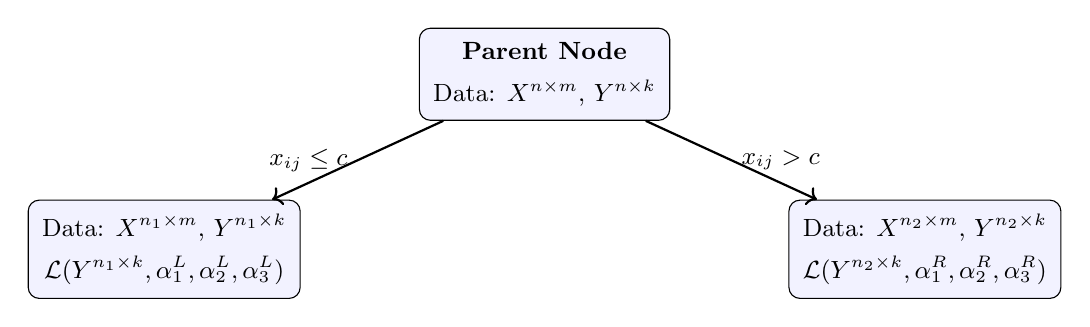
\begin{tikzpicture}[
  node distance=1cm and 1.5cm,
  every node/.style={font=\small},
  data/.style={rectangle, draw, align=center, fill=blue!5, rounded corners, inner sep=5pt},
  split/.style={->, thick}
  ]
  % Parent node
  \node[data] (parent) {
    \textbf{Parent Node} \\[0.15cm]
    Data: $X^{n \times m}$, $Y^{n \times k}$
  };
  
  % Left child
  \node[data, below left=of parent] (left) {
    Data: $X^{n_1 \times m}$, $Y^{n_1 \times k}$ \\[0.15cm]
    $\mathcal{L}(Y^{n_1 \times k}, \alpha_1^L, \alpha_2^L, \alpha_3^L)$
  };
  
  % Right  
  \node[data, below right=of parent] (right) {
    Data: $X^{n_2 \times m}$, $Y^{n_2 \times k}$ \\[0.15cm]
    $\mathcal{L}(Y^{n_2 \times k}, \alpha_1^R, \alpha_2^R, \alpha_3^R)$
  };
  
  % Arrows
  \draw[split] (parent) -- node[midway, left] {$x_{ij} \leq c$} (left);
  \draw[split] (parent) -- node[midway, right] {$x_{ij} > c$} (right);
\end{tikzpicture}

\vspace{0.5cm}



\[
(i^*, c^*) = \operatorname{argmax}_{i,c} \left( \max_{\boldsymbol{\alpha}^L} \mathcal{L}(Y^{n_1 \times k}, \boldsymbol{\alpha}^L) + \max_{\boldsymbol{\alpha}^R} \mathcal{L}(Y^{n_2 \times k}, \boldsymbol{\alpha}^R) \right)
\]
\textbf{Parameter Estimation Complexity:} $6 \times m \times p$ parameters per split:
\[
\text{Total = }6 \times m \times p =  6 \times 10 \times 10 = 600 \text{ optimizations per node}
\]
}
% \only<2>{
% For trees that can potentially grow in all directions to at least 6 levels deep, we have:
% \begin{equation}
% 3 \times m \times p \times \sum_{i=1}^{6} 2^i = 3 \times m \times p \times 126 = 378 \times m \times p
% \end{equation}
% parameters that we estimate dynamically. This number can become very large---for example, when $m=10$ and $p=10$, the total number of parameters is $378 \times 10 \times 10 = 37,800$.
% }
\only<2>{
\note{If we build a tree with just three levels — meaning a tree with 8 leaves — we already need to solve the optimization problem 4,200 times.

This is a large computational cost. And remember, trees can grow much deeper depending on the dataset. As the depth increases, the number of nodes — and therefore the number of parameter estimations — grows exponentially.}

    \centering
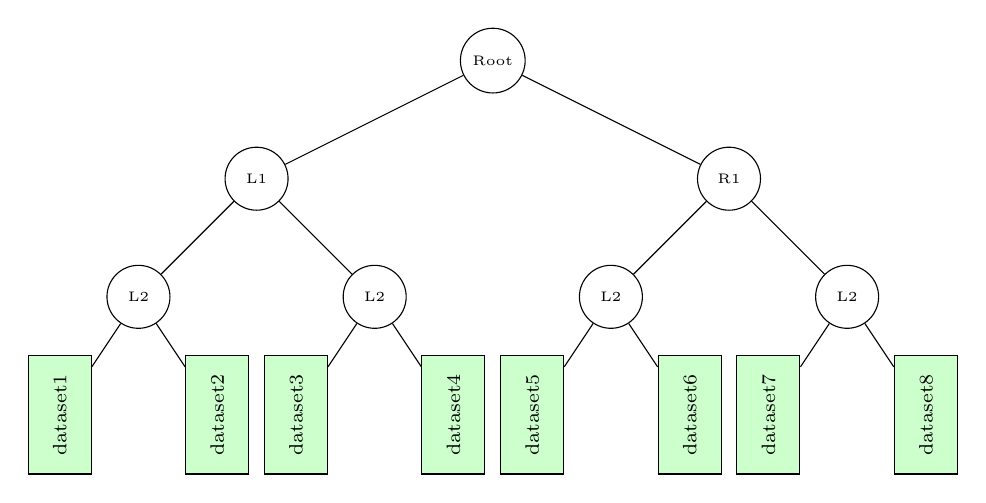
\begin{tikzpicture}[
  level/.style={sibling distance=60mm/#1},
  every node/.style={circle, draw, minimum size=8mm, font=\tiny},
  leaf/.style={rectangle, draw, fill=green!20, minimum width=15mm, minimum height=8mm, font=\scriptsize, rotate=90}
]
\node {Root}
  child {
    node {L1}
    child {
      node {L2}
      child {
        node[leaf] {dataset1}
      }
      child {
        node[leaf] {dataset2}
      }
    }
    child {
      node {L2}
      child {
        node[leaf] {dataset3}
      }
      child {
        node[leaf] {dataset4}
      }
    }
  }
  child {
    node {R1}
    child {
      node {L2}
      child {
        node[leaf] {dataset5}
      }
      child {
        node[leaf] {dataset6}
      }
    }
    child {
      node {L2}
      child {
        node[leaf] {dataset7}
      }
      child {
        node[leaf] {dataset8}
      }
    }
  };
\end{tikzpicture}

With $10$ covariates and $10$ candidates per covariate, the model requires $3 \times 10\times 10 \times (2+2^2+2^3) = 4200$ parameters, all estimated using maximum likelihood estimation. As the tree depth increases, the parameter count grows exponentially.
\note{
This tree diagram illustrates a hierarchical model designed to generate 8 subdatasets, each following a Dirichlet distribution. With 10 covariates and 10 candidates per covariate, the model requires 10×10×(2+2²+2³) = 1,400 parameters, all estimated using maximum likelihood estimation. As the tree depth increases, the parameter count grows exponentially.}
}









\only<3>{
\note{}
\boxed{
store\_samples = TRUE}
    \centering
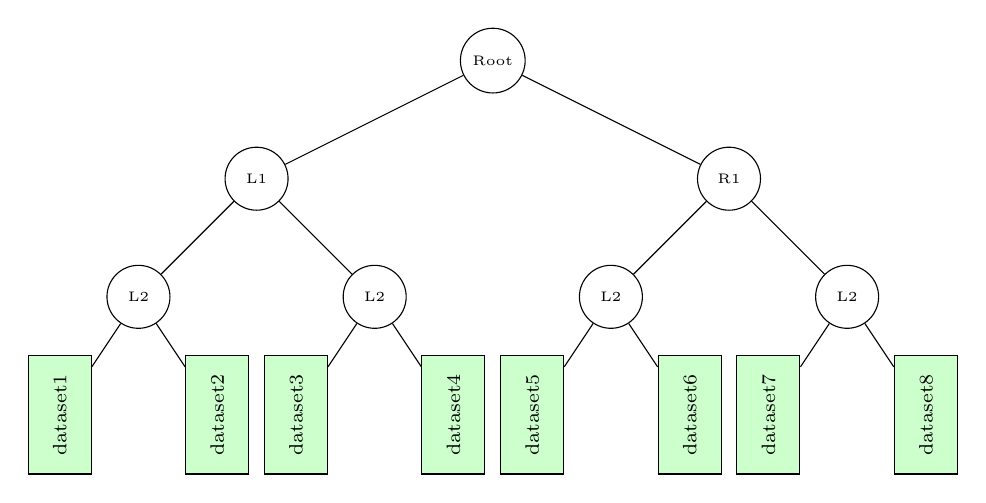
\begin{tikzpicture}[
  level/.style={sibling distance=60mm/#1},
  every node/.style={circle, draw, minimum size=8mm, font=\tiny},
  leaf/.style={rectangle, draw, fill=green!20, minimum width=15mm, minimum height=8mm, font=\scriptsize, rotate=90}
]
\node {Root}
  child {
    node {L1}
    child {
      node {L2}
      child {
        node[leaf] {dataset1}
      }
      child {
        node[leaf] {dataset2}
      }
    }
    child {
      node {L2}
      child {
        node[leaf] {dataset3}
      }
      child {
        node[leaf] {dataset4}
      }
    }
  }
  child {
    node {R1}
    child {
      node {L2}
      child {
        node[leaf] {dataset5}
      }
      child {
        node[leaf] {dataset6}
      }
    }
    child {
      node {L2}
      child {
        node[leaf] {dataset7}
      }
      child {
        node[leaf] {dataset8}
      }
    }
  };
\end{tikzpicture}


\note{
}
}

\only<4>{
\note{}
\boxed{
store\_samples = FALSE}
    \centering
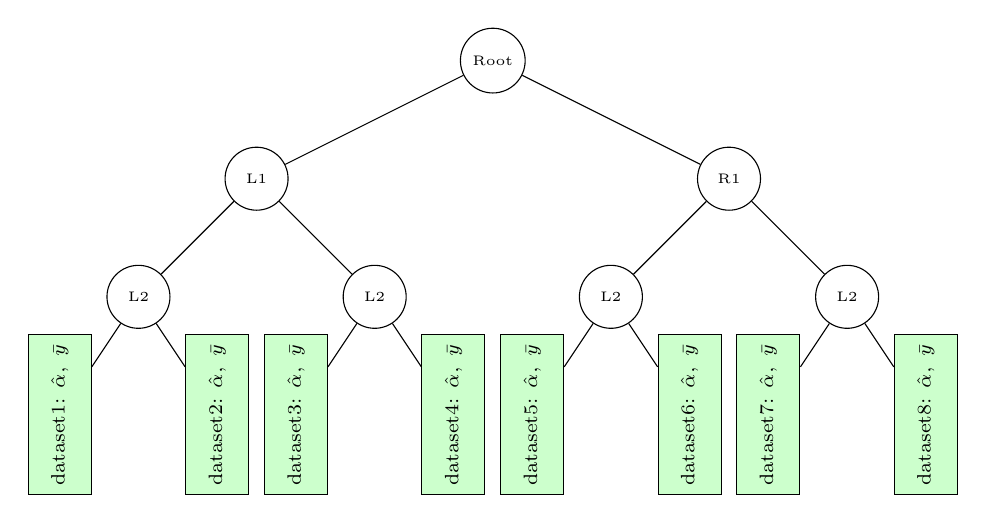
\begin{tikzpicture}[
  level/.style={sibling distance=60mm/#1},
  every node/.style={circle, draw, minimum size=8mm, font=\tiny},
  leaf/.style={rectangle, draw, fill=green!20, minimum width=15mm, minimum height=8mm, font=\scriptsize, rotate=90}
]
\node {Root}
  child {
    node {L1}
    child {
      node {L2}
      child {
        node[leaf] {dataset1: $\hat{\alpha},\,\, \bar{y}$}
      }
      child {
        node[leaf] {dataset2: $\hat{\alpha},\,\, \bar{y}$}
      }
    }
    child {
      node {L2}
      child {
        node[leaf] {dataset3: $\hat{\alpha},\,\, \bar{y}$}
      }
      child {
        node[leaf] {dataset4: $\hat{\alpha},\,\, \bar{y}$}
      }
    }
  }
  child {
    node {R1}
    child {
      node {L2}
      child {
        node[leaf] {dataset5: $\hat{\alpha},\,\, \bar{y}$}
      }
      child {
        node[leaf] {dataset6: $\hat{\alpha},\,\, \bar{y}$}
      }
    }
    child {
      node {L2}
      child {
        node[leaf] {dataset7: $\hat{\alpha},\,\, \bar{y}$}
      }
      child {
        node[leaf] {dataset8: $\hat{\alpha},\,\, \bar{y}$}
      }
    }
  };
\end{tikzpicture}

}
\end{frame}


% \only<4>{

%  This large parameter space provides the model with sufficient flexibility to accommodate diverse datasets, addressing a key limitation of traditional methods related to the Dirichlet distribution, like Dirichlet regression methods for compositional data analysis. However, this flexibility comes at a significant computational cost, rendering the approach impractical for large-scale datasets. 
% }
% \only<3>{
% The discussion of computational performance remains a significant issue for big datasets in our methodology. We have identified several promising directions for future research and performance improvements. As we discussed, MoM works well as an alternative to MLE, providing good approximations with higher computational speed. We can combine these estimation methods by selectively replacing MLE with MoM in specific nodes where we can predict the results of both methods would be similar, rather than applying MoM to all nodes.
% }



\begin{frame}
\frametitle{Distributional Dirichlet Random Forests (DRF)}
\note{
Another idea that I really like is to fit an empirical probability function.

Actually, we can fit a probability function on the training dataset. Then, for a new observation, we can evaluate this probability function to obtain its predicted distribution.

Actually, we can fit a probability function on the training dataset. This method was introduced in 2022. I will not go into the details of how it works. I have a simple example to explain it, but I will skip it to save time.
}

\begin{equation*}
P(Y = y_i \mid X = \mathbf{x}_{\text{new}}) = w_i(\mathbf{x}_{\text{new}}), \quad i = 1, \dots, n, \quad \sum_{i=1}^{n} w_i(\mathbf{x}_{\text{new}}) = 1.
\end{equation*}

\vspace{0.5em}
\begin{block}{}
The formula for the normalized weight $w_i$ is:
\[
w_i(\mathbf{x}_{\text{new}})
= \frac{1}{B} \sum_{k=1}^B 
\frac{\mathbf{1}\!\left(\mathbf{x}_{\text{new}} \in L_k(i)\right)}{|L_k(i)|}.
\]
where $|L_k(i)|$ is the size of the terminal node in tree $k$ where $\mathbf{x}_{\text{new}}$ falls.
\end{block}
\end{frame}


\begin{frame}
\frametitle{Example: Distributional Weight Calculation}
\only<1>{
\note{
Instead of explaining the full formula, let's consider a simple example. Suppose in the random forest we have only two trees, and a new observation falls into a specific leaf in each tree.  

For the first tree, the conditional probability is \(1/3\) for observations in that leaf and zero for observations not in the leaf.  
For the second tree, the conditional probability is \(1/2\).  

The final probability for the new observation is obtained by averaging over the trees.
}

\framesubtitle{Calculating weights $w_i$ for a new observation $\mathbf{x}_{\text{new}}$}

Assume $\mathbf{x}_{\text{new}}$ falls into the specified terminal nodes in $B=2$ trees.

\vspace{0.2cm}
\begin{columns}
\column{0.45\textwidth}
\centering
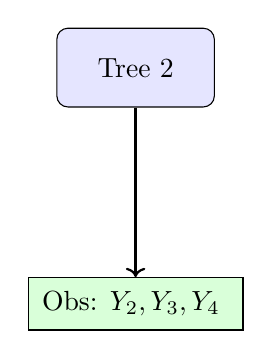
\begin{tikzpicture}[
  node distance=0.15cm,
  data/.style={rectangle, draw, align=center, fill=blue!10, minimum width=2cm, minimum height=1cm, rounded corners},
  leaf/.style={rectangle, draw, align=center, fill=green!15, minimum width=2.5cm, inner sep=5pt}
  ]
  
  \node[data] (root2) at (4, 3) {Tree 2};
  \node[leaf] (leaf2) at (4, 0) {
    Obs: $Y_2, Y_3,Y_4$
  };
  \draw[->, thick] (root2) -- (leaf2);
\end{tikzpicture}

\[
P(Y = y_i \mid \mathbf{x}_{\text{new}}) = \frac{1}{3} \, \mathbf{1}_{i \in \{2,3,4\}}
\]

\column{0.55\textwidth}
\centering
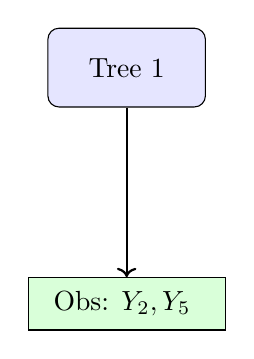
\begin{tikzpicture}[
  node distance=0.15cm,
  data/.style={rectangle, draw, align=center, fill=blue!10, minimum width=2cm, minimum height=1cm, rounded corners},
  leaf/.style={rectangle, draw, align=center, fill=green!15, minimum width=2.5cm, inner sep=5pt}
  ]
  
  \node[data] (root1) at (0, 3) {Tree 1};
  \node[leaf] (leaf1) at (0, 0) {
    Obs: $Y_2, Y_5$
  };
  \draw[->, thick] (root1) -- (leaf1);
\end{tikzpicture}

\[
P(Y = y_i \mid \mathbf{x}_{\text{new}}) = \frac{1}{2} \, \mathbf{1}_{i \in \{2,5\}}
\]
\end{columns}
}

\only<2>{
\note{
Instead of explaining the full formula, let's consider a simple example. Suppose in the random forest we have only two trees, and a new covariate falls into a specific leaf in each tree.  

For the first tree, the conditional probability is \(1/3\) for observations in that leaf and zero for observations not in the leaf.  
For the second tree, the conditional probability is \(1/2\).  

The final probability for the new observation is obtained by averaging over the trees.
}

\framesubtitle{Calculating weights $w_i$ for a new observation $\mathbf{x}_{\text{new}}$}

Assume $\mathbf{x}_{\text{new}}$ falls into the specified terminal nodes in $B=2$ trees.

\vspace{0.2cm}
\begin{columns}
\column{0.45\textwidth}
\centering
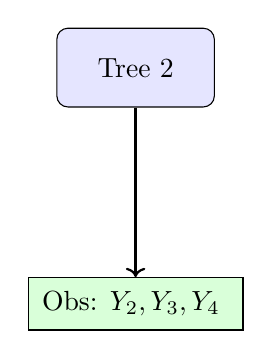
\begin{tikzpicture}[
  node distance=0.15cm,
  data/.style={rectangle, draw, align=center, fill=blue!10, minimum width=2cm, minimum height=1cm, rounded corners},
  leaf/.style={rectangle, draw, align=center, fill=green!15, minimum width=2.5cm, inner sep=5pt}
  ]
  
  \node[data] (root2) at (4, 3) {Tree 2};
  \node[leaf] (leaf2) at (4, 0) {
    Obs: $Y_2, Y_3,Y_4$
  };
  \draw[->, thick] (root2) -- (leaf2);
\end{tikzpicture}

\column{0.55\textwidth}
\centering
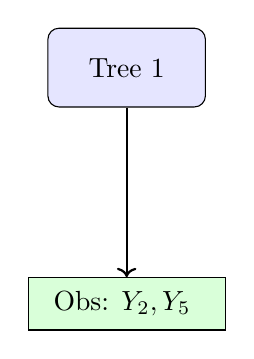
\begin{tikzpicture}[
  node distance=0.15cm,
  data/.style={rectangle, draw, align=center, fill=blue!10, minimum width=2cm, minimum height=1cm, rounded corners},
  leaf/.style={rectangle, draw, align=center, fill=green!15, minimum width=2.5cm, inner sep=5pt}
  ]
  
  \node[data] (root1) at (0, 3) {Tree 1};
  \node[leaf] (leaf1) at (0, 0) {
    Obs: $Y_2, Y_5$
  };
  \draw[->, thick] (root1) -- (leaf1);
\end{tikzpicture}
\end{columns}

\[
P(Y = y_2 \mid \mathbf{x}_{\text{new}}) = \frac{1}{2} \left( \frac{1}{3} + \frac{1}{2} \right) = \frac{5}{12}.
\]
}
\end{frame}


\begin{frame}{Inference and Prediction}
\note{
With this empirical probability function, we have flexibility for a variety of inferential statistics. For example, we can simulate new data, and also extract all the usual outputs that we would obtain from a standard random forest.

We are still exploring the use of this method to extract interesting inferential statistical results. However, we have also compared traditional prediction based on the mean function with other approaches.
}

The empirical conditional distribution:
\[
P(Y = y_i \mid X = \mathbf{x}_{\text{new}}) = w_i(\mathbf{x}_{\text{new}}), \quad i = 1, \dots, n.
\]

This allows easy computation of distributional quantities:

\begin{center}
\colorbox{green!10}{\parbox{0.5\textwidth}{
\begin{center}
\resizebox{\linewidth}{!}{%
     $\mathbb{E}(Y \mid X = \mathbf{x}_{\text{new}}) = \sum_{i=1}^{n} w_i(\mathbf{x}_{\text{new}})\, y_i$
}
\end{center}
}}
\end{center}

\begin{center}
\colorbox{green!10}{\parbox{0.5\textwidth}{
\begin{center}
\resizebox{\linewidth}{!}{%
 $P(Y \le y \mid X = \mathbf{x}_{\text{new}}) = \sum_{i: y_i \le y} w_i(\mathbf{x}_{\text{new}})$
}
\end{center}
}}
\end{center}
\end{frame}


% \begin{frame}{Improving Efficiency}
% I have worked to make the code more efficient, and it is already quite fast now. 
% To achieve even better performance, we can combine the following methods:

% \begin{enumerate}
%     \item \textbf{Distributed computing}
%     \item \textbf{Parallelisation}
%     \item \textbf{Vectorisation}
% \end{enumerate}
% \end{frame}
%follows are not a part of presentation
% 
\begin{frame}
\only<1>{
\frametitle{Dirichlet distribution}
\note{The only familiar class of distributions on simplex space is dirichlet distribution. This model operates directly on the simplex without requiring the data to be transformed into another space.
}


\vspace{1em}

\begin{center}
\colorbox{green!10}{\parbox{0.95\textwidth}{
\begin{center}
\resizebox{\linewidth}{!}{%
\[
    f_{\mathbf{Z}}((z_1,\ldots,z_k); \boldsymbol{\alpha}) = \frac{\Gamma( \alpha_0)}{\prod_{i=1}^k \Gamma(\alpha_i)} \prod_{i=1}^k z_i^{\alpha_i - 1},
\quad  z_i \in [0, 1], \quad \sum_{i=1}^k z_i = 1,
\]
}
\end{center}
}}
\end{center}

\vspace{1.5em}

\begin{itemize}[itemsep=0.8em]


\item[\textcolor{blue}{\large$\blacktriangleright$}] The sum-constant requirement of the simplex is satisfied under the Dirichlet distribution.

\item[\textcolor{blue}{\large$\blacktriangleright$}] \textbf{Extensions available:} Zero-inflated Dirichlet and Kummer–Dirichlet
\end{itemize}
}

\end{frame}
% \input{slides/bullets}
%




% \documentclass{beamer}
\usepackage{tikz}
\usetikzlibrary{shapes,arrows,positioning}

\usetheme{default}
\setbeamertemplate{navigation symbols}{}

\begin{document}

\begin{frame}{Decision Tree Prediction Methods}

\begin{columns}[T]

% Left column - Graph
\begin{column}{0.45\textwidth}
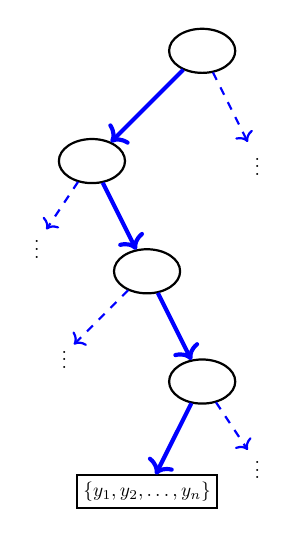
\begin{tikzpicture}[
    node/.style={ellipse, draw, minimum width=1.2cm, minimum height=0.8cm, thick},
    leaf/.style={rectangle, draw, minimum width=1.8cm, minimum height=0.6cm, thick},
    arrow/.style={->, thick, blue},
    scale=0.7,
    every node/.style={transform shape}
]

% Root node
\node[node] (root) at (0,0) {};

% Level 1
\node[node] (n1) at (-2,-2) {};
\node (dots1) at (1,-2) {\vdots};

% Level 2
\node (dots2) at (-3,-3.5) {\vdots};
\node[node] (n2) at (-1,-4) {};

% Level 3
\node (dots3) at (-2.5,-5.5) {\vdots};
\node[node] (n3) at (0,-6) {};

% Level 4
\node (dots4) at (1,-7.5) {\vdots};
\node[leaf] (leaf) at (-1,-8) {$\{y_1, y_2, \ldots, y_n\}$};

% Arrows - traversal path highlighted
\draw[arrow, line width=1.5pt] (root) -- (n1);
\draw[arrow, dashed] (root) -- (dots1);
\draw[arrow, dashed] (n1) -- (dots2);
\draw[arrow, line width=1.5pt] (n1) -- (n2);
\draw[arrow, dashed] (n2) -- (dots3);
\draw[arrow, line width=1.5pt] (n2) -- (n3);
\draw[arrow, line width=1.5pt] (n3) -- (leaf);
\draw[arrow, dashed] (n3) -- (dots4);

\end{tikzpicture}
\end{column}

% Right column - Explanation
\begin{column}{0.52\textwidth}
\small

\textbf{Process:}
\begin{enumerate}
    \item Start at root node
    \item Traverse tree based on decision rules
    \item Reach terminal node with observations
\end{enumerate}

\vspace{0.4cm}

\textbf{Default Approach:}
\begin{itemize}
    \item Mean: $\hat{y} = \frac{1}{n}\sum_{i=1}^{n} y_i$
    \item Or use Dirichlet parameters
    \item Random Forest: average across trees
\end{itemize}

\vspace{0.4cm}

\textbf{Alternative Approach:}
\begin{itemize}
    \item Collect terminal nodes from all trees
    \item Construct empirical probability function
\end{itemize}

\end{column}

\end{columns}

\end{frame}

\end{document}
%  \input{slides/centered}
%  \begin{frame}[fragile]{A slide with some code}

	\begin{columns}
		\begin{column}{0.5\linewidth}
			\footnotesize
			\begin{Verbatim}[commandchars=\\\{\}]
/* some code */
def foo(x):
  return x**0.5 + 2*x

\color{blue}/* some can be highlighted */
\color{blue}foo(3)
      \end{Verbatim}
    \end{column}
    \begin{column}{0.5\linewidth}
      {\color{red} Some explanatory text, in red, with some \texttt{monospace} text.}
      There might be some math, too:

      $$\sqrt{x} + 2x$$
    \end{column}
  \end{columns}

\end{frame}

%  \input{slides/brackets}
%  \begin{frame}{A slide with some text and a link}

  \begin{itemize}
    \item This slide has some text along with a link
      \begin{itemize}
        \item \textbf{Some bold text}: followed by an explanation
        \item \textbf{More bold text}: followed by more text
      \end{itemize}
    \item Another bullet, with sub-bullets
      \begin{itemize}
        \item A sub-bullet
        \item Another sub-bullet, with more text
      \end{itemize}
  \end{itemize}

  \vspace{2ex}
  \begin{center}
    \color{blue} \href{https://github.com/anishathalye/auriga}{github.com/anishathalye/auriga}
  \end{center}

\end{frame}








\begingroup
\setslidetemplate
\begin{frame}[t]
  \frametitle{Additive Log-Ratio (ALR) Transformation}

  \vspace{0.2cm}
\note{One of the earliest and most influential ideas was to transform the data from the simplex into real space using log-ratio transformations. Introduced By Aitchison (1982). 

One of the simplest examples is the additive log-ratio transformation, or ALR.

In this approach, we choose one component as a reference, divide the remaining components by that reference, and then take logarithms.

This maps the data into real space, where standard statistical methods become easier to apply, and the covariance matrix is full rank.

However, this comes with a limitation: the result depends on the choice of the reference component.

If we change the reference, the transformed data also change.}

  \sechead{Definition.}
  For $\mathbf{x}=(x_1,\ldots,x_K)^\top \in \mathcal{S}^{K-1}$,
  choose a reference component $x_K$:

  \vspace{0.35cm}
  \[
    \mathrm{ALR}(\mathbf{x})
    =\left(
      \log\frac{x_1}{x_K},\;
      \log\frac{x_2}{x_K},\;\ldots,\;
      \log\frac{x_{K-1}}{x_K}
    \right)
    \in \mathbb{R}^{K-1}
  \]

  \vspace{0.3cm}

  \only<1>{
    \begin{itemize}\setlength\itemsep{6pt}
      \item Maps compositional data to Euclidean space $\mathbb{R}^{K-1}$
      \item Covariance matrix becomes full rank $\Rightarrow$ standard methods applicable
      \item \textcolor{red!70!black}{Depends on choice of reference component $x_K$}
    \end{itemize}

    \vspace{0.3cm}
    \refcite{Aitchison (1982)}
  }

\end{frame}
\endgroup
 
% ══════════════════════════════════════════════════════════════
% SLIDE 2 — CLR
% ══════════════════════════════════════════════════════════════
\begingroup
\setslidetemplate
\begin{frame}[t]
  \frametitle{Centered Log-Ratio (CLR) Transformation}

  \vspace{0.2cm}
\note{To avoid this dependence, Aitchison (1982) introduced another transformation the centered log-ratio transformation, or CLR.

Here we divide each component by the geometric mean of all components.


But,  the covariance matrix remains singular, which leads us to the next transformation.}
  \sechead{Definition.}
  Normalize by the geometric mean:

  \vspace{0.3cm}
  \[
    \mathrm{CLR}(\mathbf{x})
    = \left(
      \log\frac{x_1}{g(\mathbf{x})},\ldots,
      \log\frac{x_K}{g(\mathbf{x})}
    \right)
    \in \mathbb{R}^K
  \]

  \[
    g(\mathbf{x}) = \left(\prod_{j=1}^K x_j\right)^{1/K}
  \]

  \vspace{0.2cm}

  \only<1>{
    \begin{itemize}\setlength\itemsep{6pt}
      \item Symmetric representation (no reference component)
      \item Components satisfy: $\sum_{i=1}^K \mathrm{CLR}_i = 0$
      \item Still lies in a constrained subspace $\Rightarrow$ singular covariance
    \end{itemize}

    \vspace{0.3cm}
    \refcite{Aitchison (1982)}
  }

\end{frame}
\endgroup
 
% ══════════════════════════════════════════════════════════════
% SLIDE 3 — ILR
% ══════════════════════════════════════════════════════════════
\begingroup
\setslidetemplate
\begin{frame}[t]
  \frametitle{Isometric Log-Ratio (ILR) Transformation}
  \vspace{0.2cm}
\note{To address this, one more step is added.

By projecting the CLR coordinates onto an orthonormal basis, usually with a Helmert sub-matrix, we obtain the isometric log-ratio transformation, or ILR.

This gives a representation in real Euclidean space with full rank covariance.

Among these methods, ILR is one of the most commonly used in practice.}
 
      \sechead{Definition.} (\refcite{Barceló-Vidal et al.\ (2001); Egozcue et al.\ (2003)})

      By projecting the CLR coordinates onto an orthonormal basis, usually with a $(K{-}1)\!\times\! K$ Helmert sub-matrix $\mathbf{H}$, we obtain the isometric log-ratio transformation, or ILR:
 
      \vspace{0.2cm}
      \[
        \mathrm{ILR}(\mathbf{x})
        = \mathbf{H}\;\mathrm{CLR}(\mathbf{x})
        = (z_1,\;z_2,\;\ldots,\;z_{K-1})
        \in\mathbb{R}^{K-1}
      \]
      \[
        \mathbf{H}\mathbf{H}^\top = \mathbf{I}_{K-1}
        \quad\text{(rows orthonormal)}
      \]
 \only<1>{
      \begin{alertblock}{Properties.}
      \begin{itemize}\setlength\itemsep{4pt}
        \item Resolves CLR singularity: $\Sigma_{\mathrm{ILR}}$ is \textbf{full rank}
        \item Any $(K{-}1)\!\times\!K$ orthonormal matrix works in place of $\mathbf{H}$
        \item \textcolor[HTML]{2A9D8F}{\textbf{Isometric:}} Distances preserved by $\mathbf{H}$:
          $\|\mathrm{CLR}(\mathbf{x})-\mathrm{CLR}(\mathbf{y})\| = \|\mathrm{ILR}(\mathbf{x})-\mathrm{ILR}(\mathbf{y})\|$
       
        
      \end{itemize}
      
            \end{alertblock}

 }

\end{frame}
\endgroup



\begin{frame}{One Idea: Transforming to Real Space}


\only<1>{
\note{These transformations are useful, and in many applications they work very well.

But A group of researchers strongly argued that log-ratio transformations are not just useful, but necessary for compositional data analysis.

To support this view, they introduced a set of principles that any valid method for compositional data should satisfy.


}
\begin{itemize}
    \item[1)]
    CoDA School: Some researchers claim that log-ratio transformations are necessary for compositional data.
    \item[2)]
    To support this view, a set of principles (CoDA principles) was proposed that any valid compositional method should satisfy.
\end{itemize}

  \vspace{0.2cm}
  \renewcommand{\arraystretch}{1.35}
  \setlength{\tabcolsep}{8pt}

  \begin{tabular}{>{\bfseries}l l >{\footnotesize\itshape\color{gray}}l}
    \toprule
    \rowcolor{mainblue}
    \color{white}Method &
    \color{white}Formula &
    \color{white}Reference \\
    \midrule

    \rowcolor{accentblue!20}
    ALR & $\log x_i - \log x_K$ & Aitchison (1982) \\

    \rowcolor{accentblue!20}
    CLR & $\log x_i - K^{-1}\sum_{j=1}^{K} \log y_j$ & Aitchison (1983) \\

    \rowcolor{accentblue!20}
    ILR & $\mathbf{H}\!\left(\log y_i - K^{-1}\sum_{j=1}^{K} \log y_j\right)$ & Egozcue et al.\ (2003) \\

    \midrule

    \bottomrule
  \end{tabular}

}



\only<2>{

     \note{
The three most well-known are scale invariance, permutation invariance, and subcompositional coherence.

Scale invariance means that changing the scale of the composition should not affect the result.

Permutation invariance means that the analysis should not depend on the order of the components.

And subcompositional coherence means that conclusions based on a subset of components should remain consistent with conclusions from the full composition.

Based on these principles, researchers developed new definitions of distance, geometry, and statistical operations specifically for compositional data.


I mention these principles because they appear everywhere in the compositional data literature.



I spent more than enough time trying to understand why they are important?

And I failed. I don't know what role they play in statistical analysis of compositional data.

But I realized that I'm not alone in this and that there has been a lot of disagreement about these principles and logarithmic ratio transformations.

I would like to briefly mention one smal part of that debate before moving on.



}

   \begin{alertblock}{Principles of CODA}
      \begin{itemize}
       \item 
   \textbf{scale invariance},
   \item
   \textbf{permutation invariance}, and 
   \item \textbf{subcompositional coherence}
   If \( \Delta_p(\mathbf{x}, \mathbf{y}) \) denotes a distance measure between compositions with \( p \) parts, then
    \begin{equation*}
    \Delta_k(\mathbf{x}, \mathbf{y}) \geq \Delta_d(\mathbf{x}_d, \mathbf{y}_d),
    \end{equation*}
    where \( \mathbf{x}, \mathbf{y} \) are compositions with \( k \) parts, and \( \mathbf{x}_d, \mathbf{y}_d \) are corresponding subcompositions with \( d < k \) parts.
    \end{itemize}
    \end{alertblock}

    
      \begin{itemize}
        \item[1)] \textbf{Basic mathematical operations} on the simplex (perturbation, powering, inner product)
        \item[2)] \textbf{Measures of central tendency}: simplicial means and medians

        \item[3)] \textbf{Distances and metrics} between compositions
        \item[4)] \textbf{Distributions} defined on or adapted to the simplex
      \end{itemize}
}




\end{frame}

\begin{frame}{Frame Title}

     \note{

an example of principles, personaly after one year working on this topice I still dont know which problem this principle try to solve and I am not alone in this regard. there is a long-term contrvery around this topic.

}

\[
\mathbf{T}'_4 = T\Big(\frac{Y'_1}{S'_4},\frac{Y'_2}{S'_4},\frac{Y'_3}{S'_4},\frac{Y'_4}{S'_4}\Big):(T'_1,T'_2,T'_3,T'_4)
\\
\mathbf{T}'_3 = T\Big(\frac{Y'_1}{S'_4},\frac{Y'_2}{S'_4},\frac{Y'_3}{S'_4}\Big):(T'_1,T'_2,T'_3)
\\
D_3(\mathbf{T}_3,\mathbf{T}'_3) \le D_4(\mathbf{T}_4,\mathbf{T}'_4)
\]



\end{frame}

% \begin{frame}{A Fundamental Controversy}
%     There have been long term debates between researcher in this field from the beginning sofar.

% Aitchison (1982) pioneered efforts to address the analysis of compositional data by arguing that such data should be transformed to Euclidean space using log-ratio methods.
   
%   % \bibliographystyle{plainnat}
%   % \bibliography{references} 

    
% \end{frame}
% \begin{frame}{Key Critics: D.F.\ Watson}
% \note{Wantson and philip were the first one that chalenged this principles and from 1989 to 1992 depates exchanges between them and published in... journal}

%     \textbf{Watson \& Philip (1989)} were among the \textbf{earliest} voices
%     to challenge the log-ratio framework.
%  \only<1>{
%     \vspace{0.3cm}
%     \begin{block}{Core Argument}
%       \begin{itemize}
%         \item Questioned whether \textbf{scale invariance} is a
%               fundamental requirement for compositional analysis.
%         \item If compositions are strictly defined as summing to one,
%               scale invariance is \textbf{already built in} — and imposing
%               it as a separate principle becomes circular
%         \item Their exchanges with Aitchison (1989--1992) were
%               instrumental in \emph{sharpening} the CoDa Principles,
%               even if from an adversarial position.
%       \end{itemize}
%     \end{block}}
%     \only<2>{
% \note{
% Then Aitchison used the word "Stupid" in one of his note letter and undermind Watson knowledge... this mad Watson to leave the debates.

% Then Aitchison and other new researcher developed his idea and published more paper including a book...
% }
%     \begin{alertblock}{Historical Note}
%       The debate was cut short by a notable incident: Aitchison
%       used \textbf{derogatory language} toward Watson in the
%       published exchange, which effectively ended Watson's
%       participation.
 
    
%     \end{alertblock}
 
%     \vspace{0.3cm}
%     \begin{block}{Legacy}
%       Watson's questions about scale invariance remain
%       \textbf{unresolved} and were later taken up more formally
%       by Scealy \& Welsh (2011, 2014).
%     \end{block}

%  }
% \end{frame}

% \begin{frame}{Key Critics: Zier \& Rehder (1998, 2001)}
% \note{ Zier and Rehder in 1998 to 2001 started to chalenged CoDa School principles. One interesting point was even log-ration transformations are not satosfied principles in some sense.}
%     Zier \& Rehder continued the challenge against the CoDa School,
%     focusing on \textbf{technical and foundational} issues.
%  \only<1>{
%     \vspace{0.3cm}
%     \begin{block}{Core Arguments}
%       \begin{itemize}
%         \item Challenged the mathematical definition of a

%         \item \colortext{yellow}{Pointed out that even \textbf{Aitchison's own earlier
%               work} did not strictly adhere to the current CoDa
%               definition of scale invariance}
%               \textbf{metric} within compositional data analysis
%         \item Argued that scale invariance is \textbf{problematic}
%               when compositions are strictly constrained to sum to one
        
%         \item Made the case that log-ratio methods are not the
%               \emph{only} valid approach
%       \end{itemize}
%     \end{block}
% }
% \only<2>{
% \note{Despide they made some valid points but they most of thier points were ignored partly becuase of some technical errors that they made}
%     \begin{block}{Reception by the CoDa School}
%       Despite raising \textbf{some valid points}, their criticisms
%       were \textit{dismissed relatively easily} — partly because
%       of technical errors in their own work that the CoDa School
%       used to deflect the substantive arguments.
%     \end{block}
 
 
% }
 
% \end{frame}


\begin{frame}
\begin{itemize}
    \item[\textcolor{blue}{\large$\blacktriangleright$}] These transformations were introduced by Aitchison in 1982, but the principles of CoDA have been developing over the years since then.
    \item[\textcolor{blue}{\large$\blacktriangleright$}] In 1989, Watson and Philip challenged both the log-ratio approach and the notion that these principles should be treated as universal requirements, proposing alternatives such as directional approaches.
    \item[\textcolor{blue}{\large$\blacktriangleright$}] This sparked a debate between Watson and Aitchison that unfolded over several years through a series of published exchanges in \textit{Mathematical Geology}.
    \item[\textcolor{blue}{\large$\blacktriangleright$}] What began as a methodological disagreement gradually escalated in tone, becoming increasingly confrontational.
    \item[\textcolor{blue}{\large$\blacktriangleright$}] The debate ultimately ended with Watson's withdrawal --- Aitchison's use of the word \textcolor{red}{``stupid''} to dismiss Watson's contributions led Watson to disengage from further discussion.
\end{itemize}
\end{frame}

\begin{frame}
\begin{itemize}
    \item[1.] Following this period, the CoDA framework grew increasingly dominant:
    \begin{itemize}
        \item[1.1] Aitchison continued to advance the framework through numerous publications, including an influential book.
        \item[1.2] A broader research community developed around the field that supported these principles.
    \end{itemize}
    \item[2.] As a result, alternative approaches received considerably less attention.
\end{itemize}
\end{frame}


\begin{frame}{The Controversy: To Transform or Not?}
\only<1>{
The CoDA school has redefined these principles several times in response to criticism.



        \begin{alertblock}{ (Zier & Rehder (1998, 2001))}
     They pointed out that even Aitchison’s own earlier work did not strictly satisfy the later CoDA definition of scale invariance.
    \end{alertblock}


        \begin{alertblock}{ (Scealy \& Welsh 2014)}
      The CoDa Principles act as a \textbf{gatekeeping criterion}:
      valid and useful methods have been dismissed simply for not
      conforming to them.
 
      \vspace{0.2cm}
      This is \textbf{unusual, perhaps unique, in statistical
      data analysis}.
    \end{alertblock}
}
\end{frame}



\begin{frame}{One Idea: Transforming to Real Space}


\note{
Despite the strong emphasis of the CoDA school on log-ratio transformations, they are not the only way to work with compositional data.

Several other transformations have also been developed, including approaches that are not based on logarithms and do not strictly follow the classical CoDA framework.

Some of these alternatives are listed in the table.

And in practice, depending on the data and the modeling objective, they can sometimes perform as well as — or even better than — log-ratio transformations.


Still, even when these transformations are useful, one important difficulty remains.

Once we move the data out of the simplex, interpretation becomes less direct.

Some results, such as predictions, can often be mapped back into the simplex.

But many others become much harder to interpret in the original compositional space.

So while transformation can be useful computationally, it often makes interpretation less natural.

This is one of the main reasons why working directly in the simplex can be valuable.

And this is exactly the direction we followed in the cotext of machine learning:


}

\only<1>{
  \framesubtitle{A transformation $\mathcal{S}^{K-1} \to \mathbb{R}^{K-1}$ unlocks standard inference: regression, PCA, LDA}

  \vspace{0.2cm}
  \renewcommand{\arraystretch}{1.35}
  \setlength{\tabcolsep}{8pt}

  \begin{tabular}{>{\bfseries}l l >{\footnotesize\itshape\color{gray}}l}
    \toprule
    \rowcolor{mainblue}
    \color{white}Method &
    \color{white}Formula &
    \color{white}Reference \\
    \midrule

    \rowcolor{accentblue!20}
    ALR & $\log y_i - \log y_K$ & Aitchison (1982) \\

    \rowcolor{accentblue!20}
    CLR & $\log y_i - K^{-1}\sum_{j=1}^{K} \log y_j$ & Aitchison (1983) \\

    \rowcolor{accentblue!20}
    ILR & $\mathbf{H}\!\left(\log y_i - K^{-1}\sum_{j=1}^{K} \log y_j\right)$ & Egozcue et al.\ (2003) \\

    \midrule
  
    {\normalfont $\alpha$} &
    {\footnotesize $\mathbf{H}[K_\alpha^{-1}(\mathbf{y} \otimes \alpha)]$} &
    Tsagris et al.\ (2011) \\

    {\normalfont BC$_1$} &
    {\footnotesize $\lambda^{-1}\!\left[(y_i / y_K)^\lambda - 1\right]$} &
    Aitchison (2003) \\

    {\normalfont BC$_2$} &
    {\footnotesize $\theta^{-1}(y_i^\theta - 1)$} &
    Greenacre (2010) \\

    {\normalfont Hyper-spherical} &
    {\footnotesize $\arccos\!\left(\dfrac{y_i}{\prod_{j=i+1}^{K} y_j}\right)$} &
    Wang et al.\ (2007) \\

    {\normalfont Square root} &
    {\footnotesize $\sqrt{y_i}$} &
    Stephens (1982) \\

    \bottomrule
  \end{tabular}

  \vspace{0.2cm}
  {\small\textbf{Key:} ALR, CLR, ILR are the most widely used;
  all resolve singularity of $\Sigma_{\mathbf{X}}$ by mapping to unconstrained $\mathbb{R}^{K-1}$.}
}



\end{frame}



\end{document}





% % Auriga theme
% % https://github.com/anishathalye/auriga

% \documentclass[aspectratio=169]{beamer}

% % ── Fonts & Encoding ──────────────────────────────────────────────
% \usepackage[T1]{fontenc}
% \usepackage{lmodern}

% % ── Math ──────────────────────────────────────────────────────────
% \usepackage{amsmath}
% \usepackage{amssymb}
% \usepackage{multirow}
% % ── Graphics & Color ──────────────────────────────────────────────
% \usepackage{graphicx}
% \usepackage{xcolor}
% \usepackage{colortbl}
% \usepackage{tcolorbox}

% % ── TikZ ──────────────────────────────────────────────────────────
% \usepackage{tikz}
% \usetikzlibrary{arrows.meta, calc, decorations.pathreplacing, shapes, arrows, positioning}

% % ── Plots ─────────────────────────────────────────────────────────
% \usepackage{pgfplots}
% \pgfplotsset{compat=1.18}

% % ── Tables ────────────────────────────────────────────────────────
% \usepackage{booktabs}
% \usepackage{array}

% % ── Lists & Symbols ───────────────────────────────────────────────
% \usepackage{enumitem}
% \usepackage{pifont}

% % ── References & QR ───────────────────────────────────────────────
% \usepackage{natbib}
% \usepackage{qrcode}
% \usepackage{fancyvrb}
% \usepackage{pgfpages}

% % ── Theme ─────────────────────────────────────────────────────────
% \usetheme{auriga}
% \usecolortheme{auriga}

% % ── Custom Colors ─────────────────────────────────────────────────
% \definecolor{leftblue}{RGB}{219, 234, 254}
% \definecolor{rightred}{RGB}{254, 226, 226}

% % ── Title Info ────────────────────────────────────────────────────
% \title{Towards predictive modelling of compositional data}
% \author{
%   \underline{Khaled Masoumifard}\inst{1} \and
%   Stephan van der Westhuizen\inst{1} \and
%   Sugnet Gardner-Lubbe\inst{1}
% }
% \institute[shortinst]{
%   \inst{1} Dept.\ of Statistics and Actuarial Science,
%   Stellenbosch University, Stellenbosch, South Africa
% }

% % ─────────────────────────────────────────────────────────────────
% \begin{document}
% 

  \setbeamercolor{page number in head/foot}{fg=background canvas.bg}
  \begin{frame}
    \begin{tikzpicture}[remember picture, overlay]
      \node[anchor=north west, xshift=1em, yshift=-1em] at (current page.north west) {
        
\includegraphics[width=3cm]{logo.png}
      };
    \end{tikzpicture}

    \titlepage


      \begin{center}
    %    
\includegraphics[width=0.15\linewidth]{slides/DirichletRF.jpg}
    \qrcode[height=2.8cm]{https://github.com/Xaleed/DirichletRF.git}

    \vspace{0.1cm}

    {\small GitHub repository}

  \end{center}
  \end{frame}



\begin{frame}{What is This Talk About?}
% \note{
% Good morning, and thank you for joining this talk. It is about developing DDRF, which is part of my postdoc project at Stellenbosch University, in collaboration with Stephan and Professor Lubbe.


% In a nutshell, I’ll shortly refer what composistional data is? I will explain why is it reasonable to develop a random forest model for composiational data?
% I will some comparison result?}

\vspace{2em}



\vspace{1.5em}

\begin{itemize}

  \item[\textcolor{blue}{\large$\blacktriangleright$}] \textbf{Compositional Data} -- Fundamental properties and modeling challenges
  \vspace{1em}

  \item[\textcolor{blue}{\large$\blacktriangleright$}] \textbf{Literature Review} -- Historical development and ongoing debates
  \vspace{1em}

  \item[\textcolor{blue}{\large$\blacktriangleright$}] \textbf{Machine Learning with Random Forests} -- Capturing complex relationships
  \vspace{1em}

  % \item[\textcolor{blue}{\large$\blacktriangleright$}] \textbf{Dirichlet Random Forest} -- Model formulation and motivation
  % \vspace{1em}

  \item[\textcolor{blue}{\large$\blacktriangleright$}] \textbf{Comparative Results} -- Assessing predictive performance
  \vspace{1em}

  \item[\textcolor{blue}{\large$\blacktriangleright$}] \textbf{DirichletRF R Package} -- Implementation and practical use

\end{itemize}

\vspace{2em}

\end{frame}


\begin{frame}{Compositional data}
\only<1>{


\vspace{1em}

A simplex is a convex space of all vectors with non-negative components that sum to a constant. 



\begin{center}
\colorbox{blue!10}{\parbox{0.8\textwidth}{
\begin{center}
\[
S^c_k = \left\{ (y_1, \dots, y_k)^\top \in \mathbb{R}^k \,\middle|\, y_i \geq 0, \ \sum_{i=1}^k y_i = \textcolor{blue}{c} \right\}
\]
\end{center}
}}
\end{center}



 It is common to set \(  \textcolor{blue}{c = 1} \). We refer to data from this space as \emph{compositional data}.
 

}



\only<2>{

\textbf{A practical view of compositional data}

\vspace{0.3cm}

Let $\mathbf{Y} = (Y_1, Y_2, \dots, Y_K)$ be a vector with positive components.

\vspace{0.3cm}

The compositional transformation is defined as:
\[
\mathbf{S} =
\left(
\frac{Y_1}{\sum_{i=1}^K Y_i}, \dots,
\frac{Y_K}{\sum_{i=1}^K Y_i}
\right)
\]

\vspace{0.3cm}

This vector lies in the simplex space.

\vspace{0.5cm}

However, in this transformation we lose information about the \textbf{absolute scale}, and we cannot uniquely recover the original vector.

But we preserve the \textbf{relative information}.
In particular, for any two components $i$ and $j$:
\[
\frac{Y_i}{Y_j} = \frac{S_i}{S_j}
\]





}

% \only<3>{
% \vspace{.2cm}
%    \textbf{Example}: consider 
% \(
% \mathbf{Y} = (2000, 3000, 5000),
% \)
% which represents the amount of money (in dollars) allocated to \textit{stocks}, \textit{bonds}, and \textit{cash} in an investment portfolio.  

% Then the following vector is a compositional data:
% \begin{align*}
% \scalebox{1.2}{$\left(\frac{2000}{2000+3000+5000},\;\frac{3000}{2000+3000+5000},\;\frac{5000}{2000+3000+5000}\right)$} = (0.2, 0.3, 0.5)
% \end{align*}

% \medskip

% Multiply by 100:
% \[
% 100 \cdot \mathbf{s}(\mathbf{Y}) = (20, 30, 50)
% \]

% \medskip

% Same proportions, different scale (percentages).
% \note{
% Here we see a portfolio allocation example.

% After normalization, we obtain proportions of total investment.

% Multiplying by 100 expresses them as percentages, which are more intuitive in finance.

% The relative allocation (20\%, 30\%, 50\%) remains unchanged regardless of the total invested amount.
% }
% }


\only<3>{


Consider a job application pool of $50$ applicants classified by academic background.
\vspace{0.3cm}

\begin{columns}
    \begin{column}{0.4\textwidth}
        \[
        \mathbf{Y} = (10, 15, 25)
        \]
    \end{column}
    \begin{column}{0.5\textwidth}
        \begin{tabular}{lr}
            Mathematics & 10 \\
            Statistics  & 15 \\
            Computer Science & 25 \\
        \end{tabular}
    \end{column}
\end{columns}

\vspace{0.3cm}
We normalize this vector to obtain a compositional representation:
\vspace{0.2cm}

\begin{columns}
    \begin{column}{0.5\textwidth}
        \[
        \mathbf{s}(\mathbf{Y}) = \left(\frac{10}{50}, \frac{15}{50}, \frac{25}{50}\right)
        \]
    \end{column}
    \begin{column}{0.4\textwidth}
        \[
        = (0.2, 0.3, 0.5)
        \]
        Interpreted as proportions.
    \end{column}
\end{columns}

\vspace{0.2cm}
Multiplying by $100$ gives percentages:
\vspace{0.2cm}

\begin{columns}
    \begin{column}{0.5\textwidth}
        \[
        100 \cdot \mathbf{s}(\mathbf{Y}) = (20\%, 30\%, 50\%)
        \]
    \end{column}
    \begin{column}{0.4\textwidth}
        \textbf{Key idea:} The information is identical — only the scale changes.
    \end{column}
\end{columns}


}

\end{frame}


% \begin{frame}{Statistical problems with compositional data}
% 1)spurouis corelation
% 2)The (sample) covariance matrix of the data is singular with rank equal to $D - 1$, since
% \[
% \sum_{i=1}^{D} \operatorname{cov}(y_1, y_i)
% = \operatorname{cov}\left(y_1, \sum_{i=1}^{D} y_i \right)
% = \operatorname{cov}(y_1, 1)
% = 0,
% \]
% or equivalently,
% \[
% \sum_{i=2}^{D} \operatorname{cov}(y_1, y_i)
% = -\operatorname{var}(y_1),
% \]
% where each $y_i$ is a component of the composition $\mathbf{y}$.
% 3) Evidently, the problems and issues associated
% with compositional data are too numerous to list here and this is beyond the scope of
% this review paper.

    
% \end{frame}

% \begin{frame}{What methodology is more approperiate?}
% Aitchison suugest to tranfer data...

% dicson had another idea...

% a long argue staeted between them ... and finally Aitchison used stupid word and dicson lift the discussion for evere...
% Aitchison keep continue work on his idea and bring a lot of attention this his idea so many researcher for a while tried to his idea ... 
% aclsy and .. belive this made bad effect on the the field ... and for a while many researcher tried to say you have to use transformation methods...

% They belived 
% \end{frame}




% =============================================================
%  SPURIOUS CORRELATION
%  % =============================================================
%  SPURIOUS CORRELATION
%  % =============================================================
%  SPURIOUS CORRELATION
%  \input{slides/Spurious_correlation}
% =============================================================


% ------------------------------------------------------------------
%  SLIDE 1 – Spurious Correlation (Pearson)
% ------------------------------------------------------------------

\begin{frame}{Correlation}
  \note{
Now, I extend this example to 500 different job opportunities.

In other words, I generated 500 similar datasets, although only a few rows are shown in this table. Each row represents the number of applicants for one job opportunity.

If we calculate the correlation between applicants with a Mathematics background and applicants with a Statistics background in the original count data, the result is close to zero, as you can see.

This is exactly what we expect, because the variables were generated independently.

Now, if we transform the same data into the simplex space, we obtain a very different result. The Mathematics and Statistics components become strongly negatively correlated.

So, what does this correlation actually mean? What kind of information can we extract from it?

This is not an easy question to answer.

A common mistake is to interpret this as an ordinary correlation between applicants from Mathematics and Statistics backgrounds, as we would do in a standard data table.

However, this interpretation is misleading.

These types of correlations are known as spurious correlations.

      }
\only<1>{
  \begin{columns}
    \column{0.5\textwidth}
    \textbf{Original Data (Counts)}

    \vspace{0.2cm}
    \begin{center}
    \begin{tabular}{ccc}
      \hline
      Math & Stats & CS \\
      \hline
      48  & 230 & 59  \\
      286 & 181 & 73  \\
      286 & 98  & 147 \\
      35  & 14  & 12  \\
      255 & 104 & 235 \\
      $\vdots$ & $\vdots$ & $\vdots$ \\
      \hline
    \end{tabular}
    \end{center}

    \vspace{0.2cm}
    \[
      \mathrm{corr}(\text{Math},\,\text{Stats}) = 0.087
    \]

    \column{0.5\textwidth}
    
  \end{columns}


}
\only<2>{
\begin{columns}
    \column{0.5\textwidth}
    \textbf{Original Data (Counts)}

    \vspace{0.2cm}
    \begin{center}
    \begin{tabular}{ccc}
      \hline
      Math & Stats & CS \\
      \hline
      48  & 230 & 59  \\
      286 & 181 & 73  \\
      286 & 98  & 147 \\
      35  & 14  & 12  \\
      255 & 104 & 235 \\
      $\vdots$ & $\vdots$ & $\vdots$ \\
      \hline
    \end{tabular}
    \end{center}

    \vspace{0.2cm}
    \[
      \mathrm{corr}(\text{Math},\,\text{Stats}) = 0.087
    \]

    \column{0.5\textwidth}
    \textbf{Compositional Data (Normalized to 100)}

    \vspace{0.2cm}
    \begin{center}
    \begin{tabular}{ccc}
      \hline
      Math & Stats & CS \\
      \hline
      14.2 & 68.2 & 17.5 \\
      53.0 & 33.5 & 13.5 \\
      53.9 & 18.5 & 27.7 \\
      57.4 & 23.0 & 19.7 \\
      42.9 & 17.5 & 39.6 \\
      $\vdots$ & $\vdots$ & $\vdots$ \\
      \hline
    \end{tabular}
    \end{center}

    \vspace{0.2cm}
    \[
      \mathrm{corr}(X_{\text{math}},\, X_{\text{stats}}) = -0.874
    \]
  \end{columns}

}

\end{frame}

\end{frame}
\begin{frame}{Spurious Correlation}

 


\only<1>{
\note{Remove this slide:
Spurious correlation

One important consequence of working with compositional data is spurious correlation.

This phenomenon was introduced by Pearson in 1897.

He showed that ratios that share a common denominator can appear correlated, even when the original variables are completely independent.

To see this, let us consider three independent random variables: A, B, and C.

Now suppose we construct two new variables by dividing A by C and B by C.

Even though A and B are independent, these two ratios can become correlated because they share the same denominator.

}
  \begin{block}{Pearson (1897)}
    Ratios that share a common denominator are correlated even when the
    original variables are \emph{completely independent}.
  \end{block}

  \vspace{0.4em}
  \textbf{Simple illustration:} Let $A$, $B$, $C$ be mutually independent. Then:
  \[
    \operatorname{corr}\!\left(\frac{A}{C},\;\frac{B}{C}\right) \neq 0
  \]
  \vspace{0.2em}
  The shared denominator $C$ couples the two ratios artificially.
  The observed correlation reflects the \textbf{denominator's variability},
  not any true relationship between $A$ and $B$.
}

\only<2>{
\note{Spurious correlation

One important consequence of working with compositional data is spurious correlation.

This phenomenon was introduced by Pearson in 1897.

He showed that ratios that share a common denominator can appear correlated, even when the original variables are completely independent.

To see this, let us consider three independent random variables: A, B, and C.

Now suppose we construct two new variables by dividing A by C and B by C.

Even though A and B are independent, these two ratios can become correlated because they share the same denominator.

We observe exactly the same phenomenon in compositional data.

Since all components are normalized by the same sum, a common dependency is introduced.

As a result, even if two components are independent in the original space, they may appear dependent in the simplex space.

However, this is not a mistake.

}
  \begin{block}{Pearson (1897)}
    Ratios that share a common denominator are correlated even when the
    original variables are \emph{completely independent}.
  \end{block}

  \vspace{0.4em}

  \begin{columns}[t]
    \begin{column}{0.38\textwidth}
      \textbf{Original vector:}\\[4pt]
      $\mathbf{Y} = (Y_1, Y_2, \ldots, Y_K) \in \mathbb{R}_+^K$
    \end{column}
    \begin{column}{0.58\textwidth}
      \textbf{Simplex (normalized):}\\[4pt]
      $\mathbf{s}(\mathbf{Y}) = \!\left(\dfrac{Y_1}{S},\, \dfrac{Y_2}{S},\, \ldots,\, \dfrac{Y_K}{S}\right),
      \quad S = \sum_{j=1}^{K} Y_j$
    \end{column}
  \end{columns}

  \vspace{0.5em}
  \rule{\textwidth}{0.3pt}
  \vspace{0.3em}

  Even if $\operatorname{corr}(Y_1,\, Y_2) = 0$, we usually observe:
  \[
    \boxed{\operatorname{corr}\!\left(\frac{Y_1}{S},\,\frac{Y_2}{S}\right) \neq 0}
  \]
}

\only<3>{
\note{Mathematically, everything is correct.

The problem is only interpretation.

Pearson’s warning was exactly about this point: we should not interpret correlations between ratios as correlations between the original variables.

Unfortunately, this mistake often happens in practice.

}
  \[
  \boxed{
    \operatorname{corr}\!\left(\frac{Y_1}{S}, \frac{Y_2}{S}\right)
    =
    \frac{
      \mathbb{E}\!\left(\frac{Y_1 Y_2}{S^2}\right)
      - \mathbb{E}\!\left(\frac{Y_1}{S}\right)\mathbb{E}\!\left(\frac{Y_2}{S}\right)
    }{
      \sqrt{\operatorname{Var}\!\left(\frac{Y_1}{S}\right)}\;
      \sqrt{\operatorname{Var}\!\left(\frac{Y_2}{S}\right)}
    }
  }
  \]
  \vspace{0.4em}
  \begin{block}{Pearson's warning}
    The danger arises when one interprets a correlation between ratios as evidence
    of a genuine association between the \emph{original} variables.
    Such an inference is \textbf{not justified} -- the correlation may exist
    entirely because of the shared denominator, with no signal from the data at all.
  \end{block}
}



\only<4>{
  \note{
  For example, consider a job application dataset with different academic backgrounds such as mathematics, statistics, and computer science.

In the original count data (On the left), the correlation between mathematics and statistics may be very small, close to zero.

However, after normalization to percentages — that is, after moving to the simplex space — the same variables can become strongly negatively or positively correlated.

      }

  \begin{columns}
    \column{0.5\textwidth}
    \textbf{Original Data (Counts)}

    \vspace{0.2cm}
    \begin{center}
    \begin{tabular}{ccc}
      \hline
      Math & Stats & CS \\
      \hline
      48  & 230 & 59  \\
      286 & 181 & 73  \\
      286 & 98  & 147 \\
      35  & 14  & 12  \\
      255 & 104 & 235 \\
      $\vdots$ & $\vdots$ & $\vdots$ \\
      \hline
    \end{tabular}
    \end{center}

    \vspace{0.2cm}
    \[
      \mathrm{corr}(\text{Math},\,\text{Stats}) = 0.087
    \]

    \column{0.5\textwidth}
    \textbf{Compositional Data (Normalized to 100)}

    \vspace{0.2cm}
    \begin{center}
    \begin{tabular}{ccc}
      \hline
      Math & Stats & CS \\
      \hline
      14.2 & 68.2 & 17.5 \\
      53.0 & 33.5 & 13.5 \\
      53.9 & 18.5 & 27.7 \\
      57.4 & 23.0 & 19.7 \\
      42.9 & 17.5 & 39.6 \\
      $\vdots$ & $\vdots$ & $\vdots$ \\
      \hline
    \end{tabular}
    \end{center}

    \vspace{0.2cm}
    \[
      \mathrm{corr}(X_{\text{math}},\, X_{\text{stats}}) = -0.874
    \]
  \end{columns}

  \vspace{0.3em}
  \textbf{Key message:} Spurious dependence:
  This correlation does \textbf{not} necessarily reflect a true relationship.
}

\end{frame}


% ------------------------------------------------------------------
%  SLIDE 2 – Statistical Difficulties: Singular Matrix
% ------------------------------------------------------------------
\begin{frame}{Statistical Difficulties}

\note{
Singularity of the covariance matrix

Another important consequence is that the covariance matrix is not invertible in the simplex space.

This can be shown quite easily.

Because of the constant-sum constraint, the components are not independent.

As a result, one degree of freedom is lost, and the covariance matrix becomes singular.

This creates a practical limitation.

Many standard statistical methods require the inverse of the covariance matrix, such as regression models and multivariate techniques.

Therefore, these methods cannot be directly applied to compositional data.

There are also several other difficulties that arise from working in the simplex space.

I will not go into all of them here.

However, all of these challenges motivated researchers to develop new methods specifically designed for compositional data.
}

\only<1>{
  \vspace{0.4em}
  \[
  \Sigma_{\mathbf{X}} =
  \begin{pmatrix}
    \operatorname{Var}(X_1)     & \operatorname{cov}(X_1,X_2) & \cdots & \operatorname{cov}(X_1,X_K) \\
    \operatorname{cov}(X_2,X_1) & \operatorname{Var}(X_2)     & \cdots & \operatorname{cov}(X_2,X_K) \\
    \vdots                      & \vdots                       & \ddots & \vdots \\
    \operatorname{cov}(X_K,X_1) & \operatorname{cov}(X_K,X_2) & \cdots & \operatorname{Var}(X_K)
  \end{pmatrix}
  \in \mathbb{R}^{K \times K}
  \]
  \vspace{0.2em}
  The \textbf{last row (and column) is linearly determined} by the others via the
  sum-to-constant constraint, confirming $\operatorname{rank}(\Sigma_{\mathbf{X}}) = K-1$.
}

\only<2>{
  The sum-to-constant constraint causes the \textbf{sample covariance matrix to be singular}:
  \[
    \sum_{i=1}^{K} \operatorname{cov}(X_1, X_i)
    = \operatorname{cov}\!\left(X_1,\, \sum_{i=1}^K X_i\right)
    = \operatorname{cov}(X_1,\, 1) = 0
  \]
  \[
    \Rightarrow\quad
    \sum_{i=2}^{K} \operatorname{cov}(X_1, X_i) = -\operatorname{Var}(X_1).
  \]

  \vspace{0.3em}
  $\Sigma_{\mathbf{X}}$ has rank $K-1$ $\;\Rightarrow\;$ \textbf{not invertible}.

  \vspace{0.5em}
  \begin{columns}[T]
    \begin{column}{0.48\textwidth}
      \textbf{Technical consequence:}
      \begin{itemize}
        \item Regression, LDA, and standard PCA all require $\Sigma^{-1}$ -- unavailable.
      \end{itemize}
    \end{column}
    \begin{column}{0.48\textwidth}
      \textbf{Conceptual consequence:}
      \begin{itemize}
        \item No universally accepted definition of correlation for compositional data exists yet.
      \end{itemize}
    \end{column}
  \end{columns}
}

\end{frame}


% ------------------------------------------------------------------
%  SLIDE 3 – The Log-Ratio Idea
% ------------------------------------------------------------------

% =============================================================


% ------------------------------------------------------------------
%  SLIDE 1 – Spurious Correlation (Pearson)
% ------------------------------------------------------------------

\begin{frame}{Correlation}
  \note{
Now, I extend this example to 500 different job opportunities.

In other words, I generated 500 similar datasets, although only a few rows are shown in this table. Each row represents the number of applicants for one job opportunity.

If we calculate the correlation between applicants with a Mathematics background and applicants with a Statistics background in the original count data, the result is close to zero, as you can see.

This is exactly what we expect, because the variables were generated independently.

Now, if we transform the same data into the simplex space, we obtain a very different result. The Mathematics and Statistics components become strongly negatively correlated.

So, what does this correlation actually mean? What kind of information can we extract from it?

This is not an easy question to answer.

A common mistake is to interpret this as an ordinary correlation between applicants from Mathematics and Statistics backgrounds, as we would do in a standard data table.

However, this interpretation is misleading.

These types of correlations are known as spurious correlations.

      }
\only<1>{
  \begin{columns}
    \column{0.5\textwidth}
    \textbf{Original Data (Counts)}

    \vspace{0.2cm}
    \begin{center}
    \begin{tabular}{ccc}
      \hline
      Math & Stats & CS \\
      \hline
      48  & 230 & 59  \\
      286 & 181 & 73  \\
      286 & 98  & 147 \\
      35  & 14  & 12  \\
      255 & 104 & 235 \\
      $\vdots$ & $\vdots$ & $\vdots$ \\
      \hline
    \end{tabular}
    \end{center}

    \vspace{0.2cm}
    \[
      \mathrm{corr}(\text{Math},\,\text{Stats}) = 0.087
    \]

    \column{0.5\textwidth}
    
  \end{columns}


}
\only<2>{
\begin{columns}
    \column{0.5\textwidth}
    \textbf{Original Data (Counts)}

    \vspace{0.2cm}
    \begin{center}
    \begin{tabular}{ccc}
      \hline
      Math & Stats & CS \\
      \hline
      48  & 230 & 59  \\
      286 & 181 & 73  \\
      286 & 98  & 147 \\
      35  & 14  & 12  \\
      255 & 104 & 235 \\
      $\vdots$ & $\vdots$ & $\vdots$ \\
      \hline
    \end{tabular}
    \end{center}

    \vspace{0.2cm}
    \[
      \mathrm{corr}(\text{Math},\,\text{Stats}) = 0.087
    \]

    \column{0.5\textwidth}
    \textbf{Compositional Data (Normalized to 100)}

    \vspace{0.2cm}
    \begin{center}
    \begin{tabular}{ccc}
      \hline
      Math & Stats & CS \\
      \hline
      14.2 & 68.2 & 17.5 \\
      53.0 & 33.5 & 13.5 \\
      53.9 & 18.5 & 27.7 \\
      57.4 & 23.0 & 19.7 \\
      42.9 & 17.5 & 39.6 \\
      $\vdots$ & $\vdots$ & $\vdots$ \\
      \hline
    \end{tabular}
    \end{center}

    \vspace{0.2cm}
    \[
      \mathrm{corr}(X_{\text{math}},\, X_{\text{stats}}) = -0.874
    \]
  \end{columns}

}

\end{frame}

\end{frame}
\begin{frame}{Spurious Correlation}

 


\only<1>{
\note{Remove this slide:
Spurious correlation

One important consequence of working with compositional data is spurious correlation.

This phenomenon was introduced by Pearson in 1897.

He showed that ratios that share a common denominator can appear correlated, even when the original variables are completely independent.

To see this, let us consider three independent random variables: A, B, and C.

Now suppose we construct two new variables by dividing A by C and B by C.

Even though A and B are independent, these two ratios can become correlated because they share the same denominator.

}
  \begin{block}{Pearson (1897)}
    Ratios that share a common denominator are correlated even when the
    original variables are \emph{completely independent}.
  \end{block}

  \vspace{0.4em}
  \textbf{Simple illustration:} Let $A$, $B$, $C$ be mutually independent. Then:
  \[
    \operatorname{corr}\!\left(\frac{A}{C},\;\frac{B}{C}\right) \neq 0
  \]
  \vspace{0.2em}
  The shared denominator $C$ couples the two ratios artificially.
  The observed correlation reflects the \textbf{denominator's variability},
  not any true relationship between $A$ and $B$.
}

\only<2>{
\note{Spurious correlation

One important consequence of working with compositional data is spurious correlation.

This phenomenon was introduced by Pearson in 1897.

He showed that ratios that share a common denominator can appear correlated, even when the original variables are completely independent.

To see this, let us consider three independent random variables: A, B, and C.

Now suppose we construct two new variables by dividing A by C and B by C.

Even though A and B are independent, these two ratios can become correlated because they share the same denominator.

We observe exactly the same phenomenon in compositional data.

Since all components are normalized by the same sum, a common dependency is introduced.

As a result, even if two components are independent in the original space, they may appear dependent in the simplex space.

However, this is not a mistake.

}
  \begin{block}{Pearson (1897)}
    Ratios that share a common denominator are correlated even when the
    original variables are \emph{completely independent}.
  \end{block}

  \vspace{0.4em}

  \begin{columns}[t]
    \begin{column}{0.38\textwidth}
      \textbf{Original vector:}\\[4pt]
      $\mathbf{Y} = (Y_1, Y_2, \ldots, Y_K) \in \mathbb{R}_+^K$
    \end{column}
    \begin{column}{0.58\textwidth}
      \textbf{Simplex (normalized):}\\[4pt]
      $\mathbf{s}(\mathbf{Y}) = \!\left(\dfrac{Y_1}{S},\, \dfrac{Y_2}{S},\, \ldots,\, \dfrac{Y_K}{S}\right),
      \quad S = \sum_{j=1}^{K} Y_j$
    \end{column}
  \end{columns}

  \vspace{0.5em}
  \rule{\textwidth}{0.3pt}
  \vspace{0.3em}

  Even if $\operatorname{corr}(Y_1,\, Y_2) = 0$, we usually observe:
  \[
    \boxed{\operatorname{corr}\!\left(\frac{Y_1}{S},\,\frac{Y_2}{S}\right) \neq 0}
  \]
}

\only<3>{
\note{Mathematically, everything is correct.

The problem is only interpretation.

Pearson’s warning was exactly about this point: we should not interpret correlations between ratios as correlations between the original variables.

Unfortunately, this mistake often happens in practice.

}
  \[
  \boxed{
    \operatorname{corr}\!\left(\frac{Y_1}{S}, \frac{Y_2}{S}\right)
    =
    \frac{
      \mathbb{E}\!\left(\frac{Y_1 Y_2}{S^2}\right)
      - \mathbb{E}\!\left(\frac{Y_1}{S}\right)\mathbb{E}\!\left(\frac{Y_2}{S}\right)
    }{
      \sqrt{\operatorname{Var}\!\left(\frac{Y_1}{S}\right)}\;
      \sqrt{\operatorname{Var}\!\left(\frac{Y_2}{S}\right)}
    }
  }
  \]
  \vspace{0.4em}
  \begin{block}{Pearson's warning}
    The danger arises when one interprets a correlation between ratios as evidence
    of a genuine association between the \emph{original} variables.
    Such an inference is \textbf{not justified} -- the correlation may exist
    entirely because of the shared denominator, with no signal from the data at all.
  \end{block}
}



\only<4>{
  \note{
  For example, consider a job application dataset with different academic backgrounds such as mathematics, statistics, and computer science.

In the original count data (On the left), the correlation between mathematics and statistics may be very small, close to zero.

However, after normalization to percentages — that is, after moving to the simplex space — the same variables can become strongly negatively or positively correlated.

      }

  \begin{columns}
    \column{0.5\textwidth}
    \textbf{Original Data (Counts)}

    \vspace{0.2cm}
    \begin{center}
    \begin{tabular}{ccc}
      \hline
      Math & Stats & CS \\
      \hline
      48  & 230 & 59  \\
      286 & 181 & 73  \\
      286 & 98  & 147 \\
      35  & 14  & 12  \\
      255 & 104 & 235 \\
      $\vdots$ & $\vdots$ & $\vdots$ \\
      \hline
    \end{tabular}
    \end{center}

    \vspace{0.2cm}
    \[
      \mathrm{corr}(\text{Math},\,\text{Stats}) = 0.087
    \]

    \column{0.5\textwidth}
    \textbf{Compositional Data (Normalized to 100)}

    \vspace{0.2cm}
    \begin{center}
    \begin{tabular}{ccc}
      \hline
      Math & Stats & CS \\
      \hline
      14.2 & 68.2 & 17.5 \\
      53.0 & 33.5 & 13.5 \\
      53.9 & 18.5 & 27.7 \\
      57.4 & 23.0 & 19.7 \\
      42.9 & 17.5 & 39.6 \\
      $\vdots$ & $\vdots$ & $\vdots$ \\
      \hline
    \end{tabular}
    \end{center}

    \vspace{0.2cm}
    \[
      \mathrm{corr}(X_{\text{math}},\, X_{\text{stats}}) = -0.874
    \]
  \end{columns}

  \vspace{0.3em}
  \textbf{Key message:} Spurious dependence:
  This correlation does \textbf{not} necessarily reflect a true relationship.
}

\end{frame}


% ------------------------------------------------------------------
%  SLIDE 2 – Statistical Difficulties: Singular Matrix
% ------------------------------------------------------------------
\begin{frame}{Statistical Difficulties}

\note{
Singularity of the covariance matrix

Another important consequence is that the covariance matrix is not invertible in the simplex space.

This can be shown quite easily.

Because of the constant-sum constraint, the components are not independent.

As a result, one degree of freedom is lost, and the covariance matrix becomes singular.

This creates a practical limitation.

Many standard statistical methods require the inverse of the covariance matrix, such as regression models and multivariate techniques.

Therefore, these methods cannot be directly applied to compositional data.

There are also several other difficulties that arise from working in the simplex space.

I will not go into all of them here.

However, all of these challenges motivated researchers to develop new methods specifically designed for compositional data.
}

\only<1>{
  \vspace{0.4em}
  \[
  \Sigma_{\mathbf{X}} =
  \begin{pmatrix}
    \operatorname{Var}(X_1)     & \operatorname{cov}(X_1,X_2) & \cdots & \operatorname{cov}(X_1,X_K) \\
    \operatorname{cov}(X_2,X_1) & \operatorname{Var}(X_2)     & \cdots & \operatorname{cov}(X_2,X_K) \\
    \vdots                      & \vdots                       & \ddots & \vdots \\
    \operatorname{cov}(X_K,X_1) & \operatorname{cov}(X_K,X_2) & \cdots & \operatorname{Var}(X_K)
  \end{pmatrix}
  \in \mathbb{R}^{K \times K}
  \]
  \vspace{0.2em}
  The \textbf{last row (and column) is linearly determined} by the others via the
  sum-to-constant constraint, confirming $\operatorname{rank}(\Sigma_{\mathbf{X}}) = K-1$.
}

\only<2>{
  The sum-to-constant constraint causes the \textbf{sample covariance matrix to be singular}:
  \[
    \sum_{i=1}^{K} \operatorname{cov}(X_1, X_i)
    = \operatorname{cov}\!\left(X_1,\, \sum_{i=1}^K X_i\right)
    = \operatorname{cov}(X_1,\, 1) = 0
  \]
  \[
    \Rightarrow\quad
    \sum_{i=2}^{K} \operatorname{cov}(X_1, X_i) = -\operatorname{Var}(X_1).
  \]

  \vspace{0.3em}
  $\Sigma_{\mathbf{X}}$ has rank $K-1$ $\;\Rightarrow\;$ \textbf{not invertible}.

  \vspace{0.5em}
  \begin{columns}[T]
    \begin{column}{0.48\textwidth}
      \textbf{Technical consequence:}
      \begin{itemize}
        \item Regression, LDA, and standard PCA all require $\Sigma^{-1}$ -- unavailable.
      \end{itemize}
    \end{column}
    \begin{column}{0.48\textwidth}
      \textbf{Conceptual consequence:}
      \begin{itemize}
        \item No universally accepted definition of correlation for compositional data exists yet.
      \end{itemize}
    \end{column}
  \end{columns}
}

\end{frame}


% ------------------------------------------------------------------
%  SLIDE 3 – The Log-Ratio Idea
% ------------------------------------------------------------------

% =============================================================


% ------------------------------------------------------------------
%  SLIDE 1 – Spurious Correlation (Pearson)
% ------------------------------------------------------------------

\begin{frame}{Correlation}

  
\only<1>{
  \begin{columns}
    \column{0.5\textwidth}
    \textbf{Original Data (Counts)}

    \vspace{0.2cm}
    \begin{center}
     \begin{tabular}{lccc}
      \hline
       & Math & Stats & CS \\
      \hline
      Job 1 & 48  & 230 & 59  \\
      Job 2 & 286 & 181 & 73  \\
      Job 3 & 286 & 98  & 147 \\
      Job 4 & 35  & 14  & 12  \\
      Job 5 & 255 & 104 & 235 \\
      $\vdots$ & $\vdots$ & $\vdots$ & $\vdots$ \\
      \hline
    \end{tabular}
    \end{center}

    \vspace{0.2cm}
    \[
      \mathrm{corr}(\text{Math},\,\text{Stats}) = 0.087
    \]

    \column{0.5\textwidth}
    
  \end{columns}


}
\only<2>{
\begin{columns}
    \column{0.5\textwidth}
    \textbf{Original Data (Counts)}
    \vspace{0.2cm}
    \begin{center}
    \begin{tabular}{lccc}
      \hline
       & Math & Stats & CS \\
      \hline
      Job 1 & 48  & 230 & 59  \\
      Job 2 & 286 & 181 & 73  \\
      Job 3 & 286 & 98  & 147 \\
      Job 4 & 35  & 14  & 12  \\
      Job 5 & 255 & 104 & 235 \\
      $\vdots$ & $\vdots$ & $\vdots$ & $\vdots$ \\
      \hline
    \end{tabular}
    \end{center}
    \vspace{0.2cm}
    \[
      \mathrm{corr}(\text{Math},\,\text{Stats}) = 0.087
    \]
    \column{0.5\textwidth}
    \textbf{Compositional Data (Normalized to 100)}
    \vspace{0.2cm}
    \begin{center}
    \begin{tabular}{lccc}
      \hline
       & Math & Stats & CS \\
      \hline
      Job 1 & 14.2 & 68.2 & 17.5 \\
      Job 2 & 53.0 & 33.5 & 13.5 \\
      Job 3 & 53.9 & 18.5 & 27.7 \\
      Job 4 & 57.4 & 23.0 & 19.7 \\
      Job 5 & 42.9 & 17.5 & 39.6 \\
      $\vdots$ & $\vdots$ & $\vdots$ & $\vdots$ \\
      \hline
    \end{tabular}
    \end{center}
    \vspace{0.2cm}
    \[
      \mathrm{corr}(X_{\text{math}},\, X_{\text{stats}}) = -0.874
    \]
  \end{columns}
   \vspace{0.1cm} 
What does $\mathrm{corr}(X_{\text{math}},\, X_{\text{stats}}) = -0.874$ mean? \vspace{0.1cm} 

\begin{alertblock}{Warning} A common mistake is to interpret this correlation as if it were computed on the raw counts. \end{alertblock}
}

\only<3>{
\begin{columns}
    \column{0.5\textwidth}
    \textbf{Original Data (Counts)}
    \vspace{0.2cm}
    \begin{center}
    \begin{tabular}{lccc}
      \hline
       & Math & Stats & CS \\
      \hline
      Job 1 & ?  & ? & ?  \\
      Job 2 & ? & ? & ?  \\
      Job 3 & ? & ?  & ? \\
      Job 4 & ?  & ?  & ?  \\
      Job 5 & ? & ? & ? \\
      $\vdots$ & $\vdots$ & $\vdots$ & $\vdots$ \\
      \hline
    \end{tabular}
    \end{center}
    \vspace{0.2cm}
    \[
      \mathrm{corr}(\text{Math},\,\text{Stats}) = \text{?}
    \]
    \column{0.5\textwidth}
    \textbf{Compositional Data (Normalized to 100)}
    \vspace{0.2cm}
    \begin{center}
    \begin{tabular}{lccc}
      \hline
       & Math & Stats & CS \\
      \hline
      Job 1 & 14.2 & 68.2 & 17.5 \\
      Job 2 & 53.0 & 33.5 & 13.5 \\
      Job 3 & 53.9 & 18.5 & 27.7 \\
      Job 4 & 57.4 & 23.0 & 19.7 \\
      Job 5 & 42.9 & 17.5 & 39.6 \\
      $\vdots$ & $\vdots$ & $\vdots$ & $\vdots$ \\
      \hline
    \end{tabular}
    \end{center}
    \vspace{0.2cm}
    \[
      \mathrm{corr}(X_{\text{math}},\, X_{\text{stats}}) = -0.874
    \]
  \end{columns}
  \vspace{0.1cm}
\begin{alertblock}{Warning}
In cases where only compositional data are observed, the original dependence structure is unknown and cannot be uniquely recovered from the simplex representation.\end{alertblock}
}

\end{frame}

\begin{frame}{Spurious Correlation}

 


% \only<1>{

%   \begin{block}{Pearson (1897)}
%     Ratios that share a common denominator are correlated even when the
%     original variables are \emph{completely independent}.
%   \end{block}

%   \vspace{0.4em}
%   \textbf{Simple illustration:} Let $A$, $B$, $C$ be mutually independent. Then:
%   \[
%     \operatorname{corr}\!\left(\frac{A}{C},\;\frac{B}{C}\right) \neq 0
%   \]
%   \vspace{0.2em}
%   The shared denominator $C$ couples the two ratios artificially.
%   The observed correlation reflects the \textbf{denominator's variability},
%   not any true relationship between $A$ and $B$.
% }

\only<1>{


  \begin{block}{Pearson (1897)}
    Ratios that share a common denominator are correlated even when the
    original variables are \emph{completely independent}.
  \end{block}

  \vspace{0.4em}

  \begin{columns}[t]
    \begin{column}{0.38\textwidth}
      \textbf{Original vector:}\\[4pt]
      $\mathbf{Y} = (Y_1, Y_2, \ldots, Y_K) \in \mathbb{R}_+^K$
    \end{column}
    \begin{column}{0.58\textwidth}
      \textbf{Simplex (normalized):}\\[4pt]
      $\mathbf{s}(\mathbf{Y}) = \!\left(\dfrac{Y_1}{S},\, \dfrac{Y_2}{S},\, \ldots,\, \dfrac{Y_K}{S}\right),
      \quad S = \sum_{j=1}^{K} Y_j$
    \end{column}
  \end{columns}

  \vspace{0.5em}
  \rule{\textwidth}{0.3pt}
  \vspace{0.3em}

  Even if $\operatorname{corr}(Y_1,\, Y_2) = 0$, we usually observe:
  \[
    \boxed{\operatorname{corr}\!\left(\frac{Y_1}{S},\,\frac{Y_2}{S}\right) \neq 0}
  \]
}

% \only<3>{

%   \[
%   \boxed{
%     \operatorname{corr}\!\left(\frac{Y_1}{S}, \frac{Y_2}{S}\right)
%     =
%     \frac{
%       \mathbb{E}\!\left(\frac{Y_1 Y_2}{S^2}\right)
%       - \mathbb{E}\!\left(\frac{Y_1}{S}\right)\mathbb{E}\!\left(\frac{Y_2}{S}\right)
%     }{
%       \sqrt{\operatorname{Var}\!\left(\frac{Y_1}{S}\right)}\;
%       \sqrt{\operatorname{Var}\!\left(\frac{Y_2}{S}\right)}
%     }
%   }
%   \]
%   \vspace{0.4em}
%   \begin{block}{Pearson's warning}
%     The danger arises when one interprets a correlation between ratios as evidence
%     of a genuine association between the \emph{original} variables.
%     Such an inference is \textbf{not justified} -- the correlation may exist
%     entirely because of the shared denominator, with no signal from the data at all.
%   \end{block}
% }




\end{frame}


% ------------------------------------------------------------------
%  SLIDE 2 – Statistical Difficulties: Singular Matrix
% ------------------------------------------------------------------
\begin{frame}{Statistical Difficulties}



\only<1>{
  \vspace{0.4em}
  \[
  \Sigma_{\mathbf{X}} =
  \begin{pmatrix}
    \operatorname{Var}(X_1)     & \operatorname{cov}(X_1,X_2) & \cdots & \operatorname{cov}(X_1,X_K) \\
    \operatorname{cov}(X_2,X_1) & \operatorname{Var}(X_2)     & \cdots & \operatorname{cov}(X_2,X_K) \\
    \vdots                      & \vdots                       & \ddots & \vdots \\
    \operatorname{cov}(X_K,X_1) & \operatorname{cov}(X_K,X_2) & \cdots & \operatorname{Var}(X_K)
  \end{pmatrix}
  \in \mathbb{R}^{K \times K}
  \]
  \vspace{0.2em}
  The \textbf{last row (and column) is linearly determined} by the others via the
  sum-to-constant constraint, confirming $\operatorname{rank}(\Sigma_{\mathbf{X}}) = K-1$.
}

\only<2>{
  The sum-to-constant constraint causes the \textbf{sample covariance matrix to be singular}:
  \[
    \sum_{i=1}^{K} \operatorname{cov}(X_1, X_i)
    = \operatorname{cov}\!\left(X_1,\, \sum_{i=1}^K X_i\right)
    = \operatorname{cov}(X_1,\, 1) = 0
  \]
  \[
    \Rightarrow\quad
    \sum_{i=2}^{K} \operatorname{cov}(X_1, X_i) = -\operatorname{Var}(X_1).
  \]

  \vspace{0.3em}
  $\Sigma_{\mathbf{X}}$ has rank $K-1$ $\;\Rightarrow\;$ \textbf{not invertible}.

  \vspace{0.5em}
  \begin{columns}[T]
    \begin{column}{0.48\textwidth}
      \textbf{Technical consequence:}
      \begin{itemize}
        \item Regression, LDA, and standard PCA all require $\Sigma^{-1}$ -- unavailable.
      \end{itemize}
    \end{column}
    \begin{column}{0.48\textwidth}
      \textbf{Conceptual consequence:}
      \begin{itemize}
        \item No universally accepted definition of correlation for compositional data exists yet.
      \end{itemize}
    \end{column}
  \end{columns}
}

\end{frame}


% ------------------------------------------------------------------
%  SLIDE 3 – The Log-Ratio Idea
% ------------------------------------------------------------------
\begin{frame}{Log-Ratio Transformations}
      \centering
      \vfill
      \textbf{\Large Log-Ratio Transformations}
      \vfill
\end{frame}
























\setslidetemplate
\begin{frame}[t]
  \frametitle{Additive Log-Ratio (ALR) Transformation}

  \vspace{0.2cm}



  {Definition.}
  For $\mathbf{x}=(x_1,\ldots,x_K)^\top \in \mathcal{S}^{K-1}$,
  choose a reference component $x_K$:

  \vspace{0.35cm}
  \[
    \mathrm{ALR}(\mathbf{x})
    =\left(
      \log\frac{x_1}{x_K},\;
      \log\frac{x_2}{x_K},\;\ldots,\;
      \log\frac{x_{K-1}}{x_K}
    \right)
    \in \mathbb{R}^{K-1}
  \]

  \vspace{0.3cm}

  \only<1>{
    \begin{itemize}\setlength\itemsep{6pt}
      \item Maps compositional data to Euclidean space $\mathbb{R}^{K-1}$
      \item Covariance matrix becomes full rank $\Rightarrow$ standard methods applicable
      \item \textcolor{red!70!black}{Depends on choice of reference component $x_K$}
    \end{itemize}

    \vspace{0.3cm}
    {Aitchison (1982)}
  }

\end{frame}

 
% ══════════════════════════════════════════════════════════════
% SLIDE 2 — CLR
% ══════════════════════════════════════════════════════════════

%\setslidetemplate
\begin{frame}[t]
  \frametitle{Centered Log-Ratio (CLR) Transformation}

  \vspace{0.2cm}


  {Definition.}
  Normalize by the geometric mean:

  \vspace{0.3cm}
  \[
    \mathrm{CLR}(\mathbf{x})
    = \left(
      \log\frac{x_1}{g(\mathbf{x})},\ldots,
      \log\frac{x_K}{g(\mathbf{x})}
    \right)
    \in \mathbb{R}^K
  \]

  \[
    g(\mathbf{x}) = \left(\prod_{j=1}^K x_j\right)^{1/K}
  \]

  \vspace{0.2cm}

  \only<1>{
    \begin{itemize}\setlength\itemsep{6pt}
      \item Symmetric representation (no reference component)
      \item Components satisfy: $\sum_{i=1}^K \mathrm{CLR}_i = 0$
      \item Still lies in a constrained subspace $\Rightarrow$ singular covariance
    \end{itemize}

    \vspace{0.3cm}
    {Aitchison (1982)}
  }

\end{frame}

 
% ══════════════════════════════════════════════════════════════
% SLIDE 3 — ILR
% ══════════════════════════════════════════════════════════════

%\setslidetemplate
\begin{frame}[t]
  \frametitle{Isometric Log-Ratio (ILR) Transformation}
  \vspace{0.2cm}

 
      {Definition.} ({Barceló-Vidal et al.\ (2001); Egozcue et al.\ (2003)})

      By projecting the CLR coordinates onto an orthonormal basis, usually with a $(K{-}1)\!\times\! K$ Helmert sub-matrix $\mathbf{H}$, we obtain the isometric log-ratio transformation, or ILR:
 
      \vspace{0.2cm}
      \[
        \mathrm{ILR}(\mathbf{x})
        = \mathbf{H}\;\mathrm{CLR}(\mathbf{x})
        = (z_1,\;z_2,\;\ldots,\;z_{K-1})
        \in\mathbb{R}^{K-1}
      \]
      \[
        \mathbf{H}\mathbf{H}^\top = \mathbf{I}_{K-1}
        \quad\text{(rows orthonormal)}
      \]
 \only<1>{
      \begin{alertblock}{Properties.}
      \begin{itemize}\setlength\itemsep{4pt}
        \item Resolves CLR singularity: $\Sigma_{\mathrm{ILR}}$ is \textbf{full rank}
        \item Any $(K{-}1)\!\times\!K$ orthonormal matrix works in place of $\mathbf{H}$
        \item \textcolor[HTML]{2A9D8F}{\textbf{Isometric:}} Distances preserved by $\mathbf{H}$:
          $\|\mathrm{CLR}(\mathbf{x})-\mathrm{CLR}(\mathbf{y})\| = \|\mathrm{ILR}(\mathbf{x})-\mathrm{ILR}(\mathbf{y})\|$
       
        
      \end{itemize}
      
            \end{alertblock}

 }

\end{frame}




\begin{frame}{One Idea: Transforming to Real Space}


\only<1>{


\begin{itemize}
    \item[1)]
    CoDA School: Some researchers claim that log-ratio transformations are necessary for compositional data.
    \item[2)]
    To support this view, a set of principles (CoDA principles) was proposed that any valid compositional method should satisfy.
\end{itemize}

  \vspace{0.2cm}
  \renewcommand{\arraystretch}{1.35}
  \setlength{\tabcolsep}{8pt}

  \begin{tabular}{>{\bfseries}l l >{\footnotesize\itshape\color{gray}}l}
    \toprule
    \rowcolor{mainblue}
    \color{white}Method &
    \color{white}Formula &
    \color{white}Reference \\
    \midrule

    \rowcolor{accentblue!20}
    ALR & $\log x_i - \log x_K$ & Aitchison (1982) \\

    \rowcolor{accentblue!20}
    CLR & $\log x_i - K^{-1}\sum_{j=1}^{K} \log y_j$ & Aitchison (1983) \\

    \rowcolor{accentblue!20}
    ILR & $\mathbf{H}\!\left(\log y_i - K^{-1}\sum_{j=1}^{K} \log y_j\right)$ & Egozcue et al.\ (2003) \\

    \midrule

    \bottomrule
  \end{tabular}

}



\only<2>{

 
     

   \begin{alertblock}{Principles of CODA}
      \begin{itemize}
       \item 
   \textbf{scale invariance},
   \item
   \textbf{permutation invariance}, and 
   \item \textbf{subcompositional coherence}
   If \( \Delta_p(\mathbf{x}, \mathbf{y}) \) denotes a distance measure between compositions with \( p \) parts, then
    \begin{align*}
    \Delta_k(\mathbf{x}, \mathbf{y}) \geq \Delta_d(\mathbf{x}_d, \mathbf{y}_d),
    \end{align*}
    where \( \mathbf{x}, \mathbf{y} \) are compositions with \( k \) parts, and \( \mathbf{x}_d, \mathbf{y}_d \) are corresponding subcompositions with \( d < k \) parts.
    \end{itemize}
    \end{alertblock}

    
      \begin{itemize}
        \item[1)] \textbf{Basic mathematical operations} on the simplex (perturbation, powering, inner product)
        \item[2)] \textbf{Measures of central tendency}: simplicial means and medians

        \item[3)] \textbf{Distances and metrics} between compositions
        \item[4)] \textbf{Distributions} defined on or adapted to the simplex
      \end{itemize}
}




\end{frame}



% \begin{frame}{A Fundamental Controversy}
%     There have been long term debates between researcher in this field from the beginning sofar.

% Aitchison (1982) pioneered efforts to address the analysis of compositional data by arguing that such data should be transformed to Euclidean space using log-ratio methods.
   
%   % \bibliographystyle{plainnat}
%   % \bibliography{references} 

    
% \end{frame}
% \begin{frame}{Key Critics: D.F.\ Watson}
% \note{Wantson and philip were the first one that chalenged this principles and from 1989 to 1992 depates exchanges between them and published in... journal}

%     \textbf{Watson \& Philip (1989)} were among the \textbf{earliest} voices
%     to challenge the log-ratio framework.
%  \only<1>{
%     \vspace{0.3cm}
%     \begin{block}{Core Argument}
%       \begin{itemize}
%         \item Questioned whether \textbf{scale invariance} is a
%               fundamental requirement for compositional analysis.
%         \item If compositions are strictly defined as summing to one,
%               scale invariance is \textbf{already built in} — and imposing
%               it as a separate principle becomes circular
%         \item Their exchanges with Aitchison (1989--1992) were
%               instrumental in \emph{sharpening} the CoDa Principles,
%               even if from an adversarial position.
%       \end{itemize}
%     \end{block}}
%     \only<2>{
% \note{
% Then Aitchison used the word "Stupid" in one of his note letter and undermind Watson knowledge... this mad Watson to leave the debates.

% Then Aitchison and other new researcher developed his idea and published more paper including a book...
% }
%     \begin{alertblock}{Historical Note}
%       The debate was cut short by a notable incident: Aitchison
%       used \textbf{derogatory language} toward Watson in the
%       published exchange, which effectively ended Watson's
%       participation.
 
    
%     \end{alertblock}
 
%     \vspace{0.3cm}
%     \begin{block}{Legacy}
%       Watson's questions about scale invariance remain
%       \textbf{unresolved} and were later taken up more formally
%       by Scealy \& Welsh (2011, 2014).
%     \end{block}

%  }
% \end{frame}

% \begin{frame}{Key Critics: Zier \& Rehder (1998, 2001)}
% \note{ Zier and Rehder in 1998 to 2001 started to chalenged CoDa School principles. One interesting point was even log-ration transformations are not satosfied principles in some sense.}
%     Zier \& Rehder continued the challenge against the CoDa School,
%     focusing on \textbf{technical and foundational} issues.
%  \only<1>{
%     \vspace{0.3cm}
%     \begin{block}{Core Arguments}
%       \begin{itemize}
%         \item Challenged the mathematical definition of a

%         \item \colortext{yellow}{Pointed out that even \textbf{Aitchison's own earlier
%               work} did not strictly adhere to the current CoDa
%               definition of scale invariance}
%               \textbf{metric} within compositional data analysis
%         \item Argued that scale invariance is \textbf{problematic}
%               when compositions are strictly constrained to sum to one
        
%         \item Made the case that log-ratio methods are not the
%               \emph{only} valid approach
%       \end{itemize}
%     \end{block}
% }
% \only<2>{
% \note{Despide they made some valid points but they most of thier points were ignored partly becuase of some technical errors that they made}
%     \begin{block}{Reception by the CoDa School}
%       Despite raising \textbf{some valid points}, their criticisms
%       were \textit{dismissed relatively easily} — partly because
%       of technical errors in their own work that the CoDa School
%       used to deflect the substantive arguments.
%     \end{block}
 
 
% }
 
% \end{frame}


\begin{frame}{Debates}
\begin{itemize}
    \item[\textcolor{blue}{\large$\blacktriangleright$}] These transformations were introduced by Aitchison in 1982, but the principles of CoDA have been developing over the years since then.
    \item[\textcolor{blue}{\large$\blacktriangleright$}] In 1989, Watson and Philip challenged both the log-ratio approach and the notion that these principles should be treated as universal requirements, proposing alternatives such as directional approaches.
    \item[\textcolor{blue}{\large$\blacktriangleright$}] 
    They exchanged ideas for three years, and \textit{Mathematical Geology} published their letters in response to each other.
    \item[\textcolor{blue}{\large$\blacktriangleright$}] What began as a methodological disagreement gradually escalated in tone, becoming increasingly confrontational.
    \item[\textcolor{blue}{\large$\blacktriangleright$}] The debate ultimately ended with Watson's withdrawal --- Aitchison's use of the word \textcolor{red}{``stupid''} to dismiss Watson's contributions led Watson to disengage from further discussion.
\end{itemize}
\end{frame}

\begin{frame}{Debates}
\only<1>{
     Following this period, the CoDA framework grew increasingly dominant:
    \begin{itemize}
        \item[1.1] Aitchison continued to advance the framework through numerous publications, including an influential book.
        \item[1.2] A broader research community developed around the field that supported these principles.
    \end{itemize}


      \vspace{0.2cm}

    As a result, alternative approaches received considerably less attention.
}
\only<2>{
     Following this period, the CoDA framework grew increasingly dominant:
    \begin{itemize}
        \item[1.1] Aitchison continued to advance the framework through numerous publications, including an influential book.
        \item[1.2] A broader research community developed around the field that supported these principles.
    \end{itemize}


      \vspace{0.2cm}

    As a result, alternative approaches received considerably less attention.
\centering
    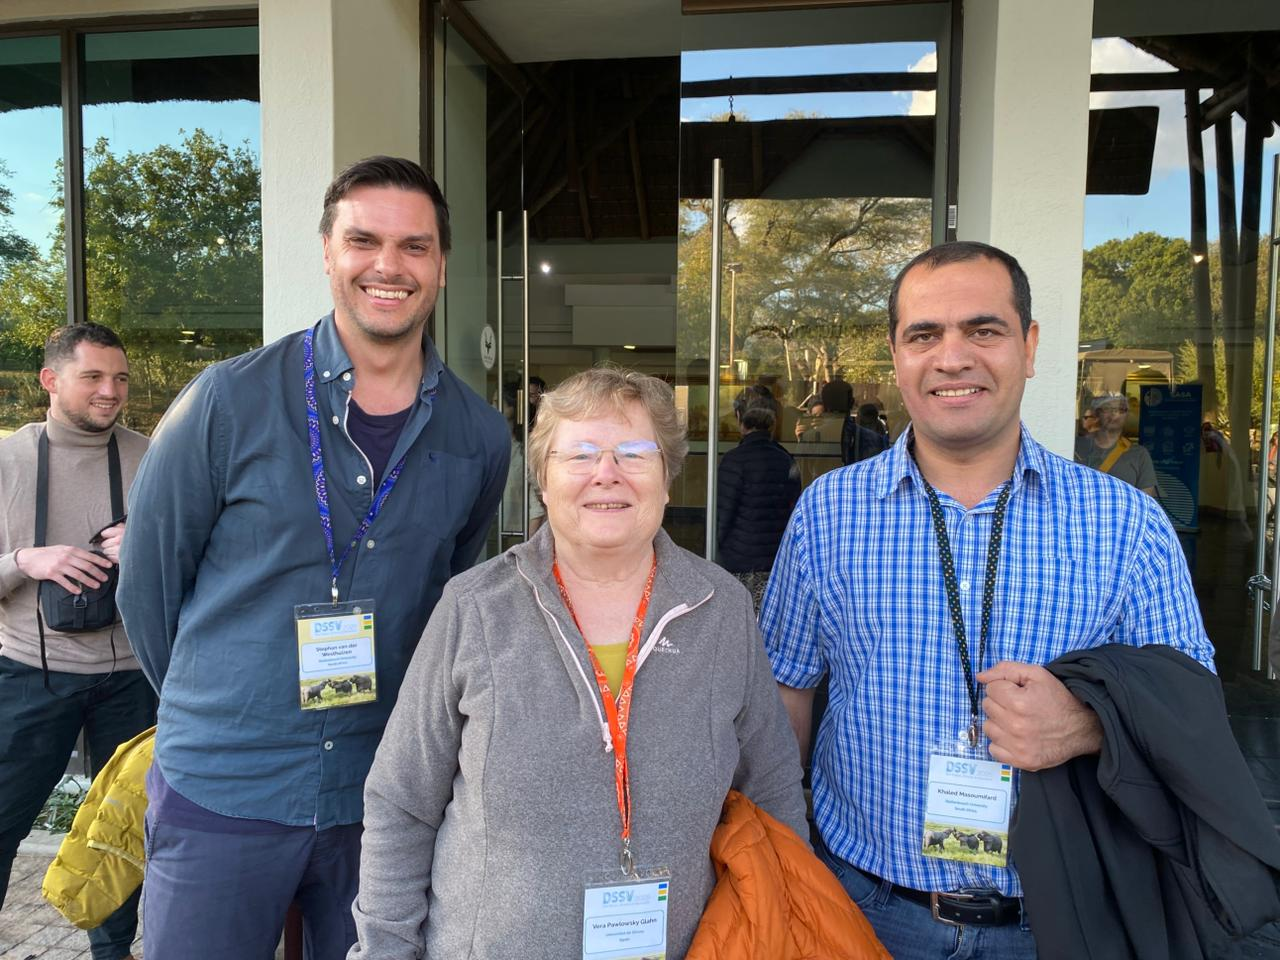
\includegraphics[width=0.4\linewidth]{slides/Vera.jpg}
}
\end{frame}


\begin{frame}{Debates}
\only<1>{
The CoDA school has redefined these principles several times in response to criticism.



        \begin{alertblock}{ (Zier \& Rehder (1998, 2001))}
     They pointed out that even Aitchison’s own earlier work did not strictly satisfy the later CoDA definition of scale invariance.
    \end{alertblock}


        \begin{alertblock}{ (Scealy \& Welsh 2014)}
      The CoDa Principles act as a \textbf{gatekeeping criterion}:
      valid and useful methods have been dismissed simply for not
      conforming to them.
 
      \vspace{0.2cm}
      This is \textbf{unusual, perhaps unique, in statistical
      data analysis}.
    \end{alertblock}
}
\end{frame}



\begin{frame}{One Idea: Transforming to Real Space}





\only<1>{
  \framesubtitle{A transformation $\mathcal{S}^{K-1} \to \mathbb{R}^{K-1}$ unlocks standard inference: regression, PCA, LDA}

  \vspace{0.2cm}
  \renewcommand{\arraystretch}{1.35}
  \setlength{\tabcolsep}{8pt}

  \begin{tabular}{>{\bfseries}l l >{\footnotesize\itshape\color{gray}}l}
    \toprule
    \rowcolor{mainblue}
    \color{white}Method &
    \color{white}Formula &
    \color{white}Reference \\
    \midrule

    \rowcolor{accentblue!20}
    ALR & $\log y_i - \log y_K$ & Aitchison (1982) \\

    \rowcolor{accentblue!20}
    CLR & $\log y_i - K^{-1}\sum_{j=1}^{K} \log y_j$ & Aitchison (1983) \\

    \rowcolor{accentblue!20}
    ILR & $\mathbf{H}\!\left(\log y_i - K^{-1}\sum_{j=1}^{K} \log y_j\right)$ & Egozcue et al.\ (2003) \\

    \midrule
  
    {\normalfont $\alpha$} &
    {\footnotesize $\mathbf{H}[K_\alpha^{-1}(\mathbf{y} \otimes \alpha)]$} &
    Tsagris et al.\ (2011) \\

    {\normalfont BC$_1$} &
    {\footnotesize $\lambda^{-1}\!\left[(y_i / y_K)^\lambda - 1\right]$} &
    Aitchison (2003) \\

    {\normalfont BC$_2$} &
    {\footnotesize $\theta^{-1}(y_i^\theta - 1)$} &
    Greenacre (2010) \\

    {\normalfont Hyper-spherical} &
    {\footnotesize $\arccos\!\left(\dfrac{y_i}{\prod_{j=i+1}^{K} y_j}\right)$} &
    Wang et al.\ (2007) \\

    {\normalfont Square root} &
    {\footnotesize $\sqrt{y_i}$} &
    Stephens (1982) \\

    \bottomrule
  \end{tabular}

  \vspace{0.2cm}
  {\small\textbf{Key:} ALR, CLR, ILR are the most widely used;
  all resolve singularity of $\Sigma_{\mathbf{X}}$ by mapping to unconstrained $\mathbb{R}^{K-1}$.}
}



\end{frame}








\begin{frame}{Machine learning for CoDA}
      \centering
      \vfill
      \textbf{\Large Machine learning for CoDA}
      \vfill
\end{frame}







\begin{frame}{Machine learning: Random Forest}

\begin{itemize}

\item \textbf{Why machine learning?}  
For responses that are compositional: many predictors with complex non-linear patterns that traditional models cannot capture.

\item \textbf{Common approaches}:  
Apply ML models without considering the simplex geometry, or transform data (with log-ratio transformations) to real space (risking distortion and bias).

\item \textbf{Why Random Forests?}  
RFs are flexible and their splitting rules can be easily adapted to respect the simplex structure.

\item PhD of van der Westhuizen (2024) inspired the idea to use tree splitting to account for coDA
\end{itemize}

    
\end{frame}



\begin{frame}{Random Forests framework}
 
\begin{itemize}
   \item[\textcolor{blue}{\large$\blacktriangleright$}]  Given a sample size $n$ and $m$ covariates:
    \[
        \mathbf{X} \in \mathbb{R}^{n \times m} \quad \text{(covariate matrix)}, \qquad
        \mathbf{Y} \in \mathbb{R}^{n \times k} \quad \text{(response matrix)}
    \]
    
  \item[\textcolor{blue}{\large$\blacktriangleright$}]  Each row of \( \mathbf{Y} \) is a compositional vector:
    \[
        Y_{i,j} > 0 \quad \text{for all } i, j, \qquad \sum_{j=1}^k Y_{i,j} = 1
    \]
        
  
     \item[\textcolor{blue}{\large$\blacktriangleright$}] Goal: learn a mapping
    \[
    \mathbf{x} \;\longrightarrow\; \mathbf{y}
    \]
    respecting the simplex geometry
    \vspace{0.8em}

    % \item[\textcolor{blue}{\large$\blacktriangleright$}] Approach: adapt \textbf{random forests} for compositional outputs
    % \vspace{0.8em}

     \item[\textcolor{blue}{\large$\blacktriangleright$}] After training:
    \begin{itemize}
        \item Predict compositional responses for new inputs
        \item Estimate conditional distribution of responses
    \end{itemize}

\end{itemize}
\end{frame}

\begin{frame}{Random Forest: Overview}

A \textbf{Random Forest} is an ensemble of decision trees, each trained on a
bootstrap sample of the data. Key tuning parameters include:

\vspace{0.5em}

\begin{itemize}
    \item \textbf{Number of trees} ($B$): more trees improve stability but increase cost
    \item \textbf{Tree depth} ($d_{\max}$): controls model complexity and overfitting
    \item \textbf{Minimum node size} ($n_{\min}$): minimum observations required to split a node
    \item \textbf{Covariates per split} ($m_{\text{try}}$): number of randomly selected covariates
    considered at each split; typically set to $\sqrt{p}$
\end{itemize}

\end{frame}

\begin{frame}{Random forest: tree}

\centering
\only<1>{

\begin{columns}
    \begin{column}{0.4\linewidth}
    
        \begin{figure}[h]
\centering
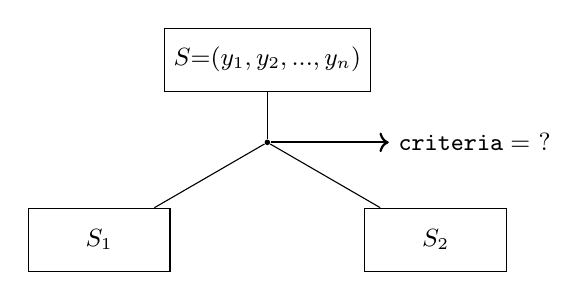
\begin{tikzpicture}[
    node distance=0.8cm,
    box/.style={rectangle, draw, minimum width=1.8cm, minimum height=0.8cm, text centered, font=\small},
    dot/.style={circle, fill=black, minimum size=2pt, inner sep=0pt},
    arrow/.style={->, thick}
]
% Main parent node
\node[box] (parent) {$S$=\\$(y_1, y_2, ..., y_n)$};
% Split point (dot in the middle)
\node[dot, below=0.6cm of parent] (split) {};
% Two child nodes
\node[box, below left=0.8cm and 1.2cm of split] (left) {$S_1$};
\node[box, below right=0.8cm and 1.2cm of split] (right) {$S_2$};
% Connections
\draw (parent) -- (split);
\draw (split) -- (left);
\draw (split) -- (right);
% Loss function arrow and equation
\node[right=1.5cm of split, font=\small] (loss) {$\texttt{criteria} = $ ?};
\draw[arrow] (split) -- (loss);
\end{tikzpicture}

\label{fig:decision_tree_split}
\end{figure}



    \end{column}
\begin{column}{0.6\linewidth}
\vspace{1cm}
$\qquad \qquad$A binary decision tree
\vspace

\resizebox{1\linewidth}{!}{%
        \begin{tikzpicture}[
  level/.style={sibling distance=60mm/#1},
  every node/.style={circle, draw, minimum size=8mm, font=\tiny},
  dots/.style={draw=none, font=\large}
]
\node {Root}
  child {
    node {L1}
    child {
      node {L2}
      child {
        node[dots] {$\vdots$}
      }
      child {
        node[dots] {$\vdots$}
      }
    }
    child {
      node {L2}
      child {
        node[dots] {$\vdots$}
      }
      child {
        node[dots] {$\vdots$}
      }
    }
  }
  child {
    node {R1}
    child {
      node {L2}
      child {
        node[dots] {$\vdots$}
      }
      child {
        node[dots] {$\vdots$}
      }
    }
    child {
      node {L2}
      child {
        node[dots] {$\vdots$}
      }
      child {
        node[dots] {$\vdots$}
      }
    }
  };
\end{tikzpicture}}
    \end{column}

    
\end{columns}


}

\end{frame}






\begin{frame}{}\only<1>{\frametitle{MSE splitting}

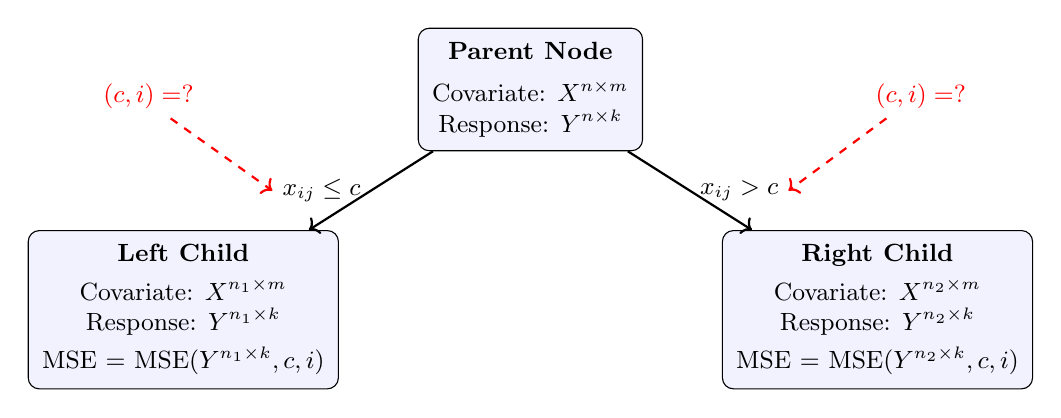
\begin{tikzpicture}[
  node distance=1cm and 1cm,
  every node/.style={font=\small},
  data/.style={rectangle, draw, align=center, fill=blue!5, rounded corners, inner sep=5pt},
  split/.style={->, thick},
  highlight/.style={->, red, thick, dashed}
  ]
  % Parent node
  \node[data] (parent) {
    \textbf{Parent Node} \\[0.15cm]
    Covariate: $X^{n \times m}$ \\ 
    Response: $Y^{n \times k}$
  };
  % Left child
  \node[data, below left=of parent] (left) {
    \textbf{Left Child} \\[0.1cm]
    Covariate: $X^{n_1 \times m}$ \\
    Response: $Y^{n_1 \times k}$ \\[0.1cm]
    MSE = $\text{MSE}(Y^{n_1 \times k},c,i)$
  };
  % Right child
  \node[data, below right=of parent] (right) {
    \textbf{Right Child} \\[0.1cm]
    Covariate: $X^{n_2 \times m}$ \\
    Response: $Y^{n_2 \times k}$ \\[0.1cm]
    MSE = $\text{MSE}(Y^{n_2 \times k},c,i)$
  };
  % Arrows
  \draw[split] (parent) -- node[midway, left] (leftlabel) {$x_{ij} \leq c$} (left);
  \draw[split] (parent) -- node[midway, right] (rightlabel) {$x_{ij} > c$} (right);
  
  % Optimize labels
  \node[red, left] (opt_i) at ([xshift=-1.5cm, yshift=1.2cm]leftlabel) {\textbf{ } $(c,i)=?$};
  \node[red, right] (opt_c) at ([xshift=1.5cm, yshift=1.2cm]rightlabel) {\textbf{} $(c,i)=?$};
  
  % Short highlight arrows from labels to split conditions
  \draw[highlight] (opt_i) -- (leftlabel.west);
  \draw[highlight] (opt_c) -- (rightlabel.east);
\end{tikzpicture}


}
\only<2>{

\frametitle{Split rule}
\begin{columns}[T]

  \column{0.8\textwidth}
 \begin{center}
\renewcommand{\arraystretch}{1.6}
\begin{tabular}{c|c>{\columncolor{purple!20}}cc>{\columncolor{purple!20}}cc|ccc|c}
\textbf{obs} & $x_1$ & \cellcolor{purple!50}$x_2$ & $x_3$ & \cellcolor{purple!20}$x_4$ & $x_5$ & $y_1$ & $y_2$ & $y_3$ & \textbf{child} \\
\hline
\rowcolor{blue!15}
1 & 0.8 & \textbf{1.2} & 3.4 & 0.5 & 2.1 & 0.60 & 0.25 & 0.15 & \textcolor{blue!80!black}{$\leftarrow$ left} \\
\rowcolor{blue!15}
2 & 2.3 & \textbf{2.7} & 1.1 & 4.2 & 0.9 & 0.10 & 0.70 & 0.20 & \textcolor{blue!80!black}{$\leftarrow$ left} \\
\rowcolor{blue!15}
3 & 1.5 & \textbf{3.1} & 2.9 & 1.8 & 3.3 & 0.45 & 0.45 & 0.10 & \textcolor{blue!80!black}{$\leftarrow$ left} \\
\rowcolor{red!15}
4 & 3.9 & \textbf{4.4} & 0.7 & 3.1 & 1.4 & 0.05 & 0.15 & 0.80 & \textcolor{red!80!black}{right $\rightarrow$} \\
\rowcolor{blue!15}
5 & 0.4 & \textbf{2.0} & 4.5 & 2.7 & 5.0 & 0.50 & 0.30 & 0.20 & \textcolor{blue!80!black}{$\leftarrow$ left} \\
\rowcolor{red!15}
6 & 2.1 & \textbf{5.6} & 3.8 & 0.3 & 2.2 & 0.02 & 0.08 & 0.90 & \textcolor{red!80!black}{right $\rightarrow$} \\
\rowcolor{red!15}
7 & 3.3 & \textbf{3.8} & 1.6 & 4.9 & 0.6 & 0.03 & 0.12 & 0.85 & \textcolor{red!80!black}{right $\rightarrow$} \\
\rowcolor{blue!15}
8 & 1.1 & \textbf{1.5} & 2.2 & 1.1 & 4.4 & 0.55 & 0.35 & 0.10 & \textcolor{blue!80!black}{$\leftarrow$ left} \\
\end{tabular}
\end{center}

  \column{0.22\textwidth}
  \vspace{1em}
  \begin{block}{Partition rule}
    Covariate 2: $i=2$ \\ Split value: $c =3.1$\\
    
  \end{block}
  \vspace{0.8em}
  \textcolor{blue!80!black}{\textbf{Left}} \\
  \hspace{0.5em} $x_2 \leq 3.1$ \\[0.2em]
  \hspace{0.5em} obs: 1, 2, 3, 5, 8 \\[0.6em]
  \textcolor{red!80!black}{\textbf{Right}} \\
   \hspace{0.5em} $x_2 > 3.1$ \\
  \hspace{0.5em} obs: 4, 6, 7


\end{columns}
}


\end{frame}




% %--- SLIDE 1: The data ---
% \begin{frame}{Growing a Tree: The Data}
% \begin{columns}[T]

%   \column{0.65\textwidth}
%   \begin{center}
%   \renewcommand{\arraystretch}{1.6}
%   \begin{tabular}{c|ccccc|ccc}
%   \textbf{obs} & $x_1$ & $x_2$ & $x_3$ & $x_4$ & $x_5$ & $y_1$ & $y_2$ & $y_3$ \\
%   \hline
%   1 & 0.8 & 1.2 & 3.4 & 0.5 & 2.1 & 0.60 & 0.25 & 0.15 \\
%   2 & 2.3 & 2.7 & 1.1 & 4.2 & 0.9 & 0.10 & 0.70 & 0.20 \\
%   3 & 1.5 & 3.1 & 2.9 & 1.8 & 3.3 & 0.45 & 0.45 & 0.10 \\
%   4 & 3.9 & 4.4 & 0.7 & 3.1 & 1.4 & 0.05 & 0.15 & 0.80 \\
%   5 & 0.4 & 2.0 & 4.5 & 2.7 & 5.0 & 0.50 & 0.30 & 0.20 \\
%   6 & 2.1 & 5.6 & 3.8 & 0.3 & 2.2 & 0.02 & 0.08 & 0.90 \\
%   7 & 3.3 & 3.8 & 1.6 & 4.9 & 0.6 & 0.03 & 0.12 & 0.85 \\
%   8 & 1.1 & 1.5 & 2.2 & 1.1 & 4.4 & 0.55 & 0.35 & 0.10 \\
%   \end{tabular}
%   \end{center}

%   \column{0.32\textwidth}
%   \vspace{1em}
%   \begin{block}{Setup}
%     Each node holds $n$ observations with $p$ covariates.
%   \end{block}
%   \vspace{0.8em}
%   \textbf{Response} $\mathbf{y}$ is compositional:
%   \[
%     \mathbf{y} = (y_1, y_2, y_3)
%   \]
%   \[
%     y_k \geq 0, \quad \textstyle\sum_k y_k = 1
%   \]
%   \vspace{0.4em}
%   Lives on the simplex $\mathcal{S}^2$.

% \end{columns}
% \end{frame}


% %--- SLIDE 2: Select covariates ---
% \begin{frame}{Step 1 — Select Covariates}
% \begin{columns}[T]

%   \column{0.65\textwidth}
%   \begin{center}
%   \renewcommand{\arraystretch}{1.6}
%   \begin{tabular}{c|c>{\columncolor{purple!20}}cc>{\columncolor{purple!20}}cc|ccc}
%   \textbf{obs} & $x_1$ & \cellcolor{purple!50}$x_2$ & $x_3$ & \cellcolor{purple!50}$x_4$ & $x_5$ & $y_1$ & $y_2$ & $y_3$ \\
%   \hline
%   1 & 0.8 & 1.2 & 3.4 & 0.5 & 2.1 & 0.60 & 0.25 & 0.15 \\
%   2 & 2.3 & 2.7 & 1.1 & 4.2 & 0.9 & 0.10 & 0.70 & 0.20 \\
%   3 & 1.5 & 3.1 & 2.9 & 1.8 & 3.3 & 0.45 & 0.45 & 0.10 \\
%   4 & 3.9 & 4.4 & 0.7 & 3.1 & 1.4 & 0.05 & 0.15 & 0.80 \\
%   5 & 0.4 & 2.0 & 4.5 & 2.7 & 5.0 & 0.50 & 0.30 & 0.20 \\
%   6 & 2.1 & 5.6 & 3.8 & 0.3 & 2.2 & 0.02 & 0.08 & 0.90 \\
%   7 & 3.3 & 3.8 & 1.6 & 4.9 & 0.6 & 0.03 & 0.12 & 0.85 \\
%   8 & 1.1 & 1.5 & 2.2 & 1.1 & 4.4 & 0.55 & 0.35 & 0.10 \\
%   \end{tabular}
%   \end{center}

%   \column{0.32\textwidth}
%   \vspace{1em}
%   \begin{block}{Random subspace}
%     At each node, draw $m \leq p$ covariates at random.
%   \end{block}
%   \vspace{0.8em}
%   \textcolor{purple!80!black}{\textbf{Selected:}} $x_2,\, x_4$
%   \vspace{0.6em}

%   \begin{itemize}[label={\ding{226}}]
%     \item Reduces correlation between trees
%     \item Only \textcolor{purple!80!black}{highlighted columns} are split candidates
%     \item Other columns are ignored at this node
%   \end{itemize}

% \end{columns}
% \end{frame}


% %--- SLIDE 3: Find the best split ---
% \begin{frame}{Step 2 — Find the Best Split}
% \begin{columns}[T]

%   \column{0.72\textwidth}
%   \begin{center}
%   \renewcommand{\arraystretch}{1.6}
%   \begin{tabular}{c|c>{\columncolor{purple!20}}cc>{\columncolor{purple!20}}cc|ccc|c}
%   \textbf{obs} & $x_1$ & \cellcolor{purple!50}$x_2$ & $x_3$ & \cellcolor{purple!20}$x_4$ & $x_5$ & $y_1$ & $y_2$ & $y_3$ & \\
%   \hline
%   \rowcolor{leftblue}
%   1 & 0.8 & \textbf{1.2} & 3.4 & 0.5 & 2.1 & 0.60 & 0.25 & 0.15 & \textcolor{blue!80!black}{$\leftarrow$ left} \\
%   \rowcolor{leftblue}
%   2 & 2.3 & \textbf{2.7} & 1.1 & 4.2 & 0.9 & 0.10 & 0.70 & 0.20 & \textcolor{blue!80!black}{$\leftarrow$ left} \\
%   \rowcolor{leftblue}
%   3 & 1.5 & \textbf{3.1} & 2.9 & 1.8 & 3.3 & 0.45 & 0.45 & 0.10 & \textcolor{blue!80!black}{$\leftarrow$ left} \\
%   \rowcolor{rightred}
%   4 & 3.9 & \textbf{4.4} & 0.7 & 3.1 & 1.4 & 0.05 & 0.15 & 0.80 & \textcolor{red!80!black}{right $\rightarrow$} \\
%   \rowcolor{leftblue}
%   5 & 0.4 & \textbf{2.0} & 4.5 & 2.7 & 5.0 & 0.50 & 0.30 & 0.20 & \textcolor{blue!80!black}{$\leftarrow$ left} \\
%   \rowcolor{rightred}
%   6 & 2.1 & \textbf{5.6} & 3.8 & 0.3 & 2.2 & 0.02 & 0.08 & 0.90 & \textcolor{red!80!black}{right $\rightarrow$} \\
%   \rowcolor{rightred}
%   7 & 3.3 & \textbf{3.8} & 1.6 & 4.9 & 0.6 & 0.03 & 0.12 & 0.85 & \textcolor{red!80!black}{right $\rightarrow$} \\
%   \rowcolor{leftblue}
%   8 & 1.1 & \textbf{1.5} & 2.2 & 1.1 & 4.4 & 0.55 & 0.35 & 0.10 & \textcolor{blue!80!black}{$\leftarrow$ left} \\
%   \end{tabular}
%   \end{center}

%   \column{0.25\textwidth}
%   \vspace{1em}
%   \begin{block}{Partition rule}
%     \textcolor{purple!80!black}{Best:} $x_2 \leq 3.5$
%   \end{block}
%   \vspace{0.8em}
%   \textcolor{blue!80!black}{\textbf{Left}} \hfill $x_2 \leq 3.5$\\[0.2em]
%   \hspace{0.5em} obs: 1,2,3,5,8 \\[0.6em]
%   \textcolor{red!80!black}{\textbf{Right}} \hfill $x_2 > 3.5$ \\[0.2em]
%   \hspace{0.5em} obs: 4,6,7
%   \vspace{0.6em}



% \end{columns}
% \end{frame}





\begin{frame}{}\only<1>{\frametitle{MSE splitting}

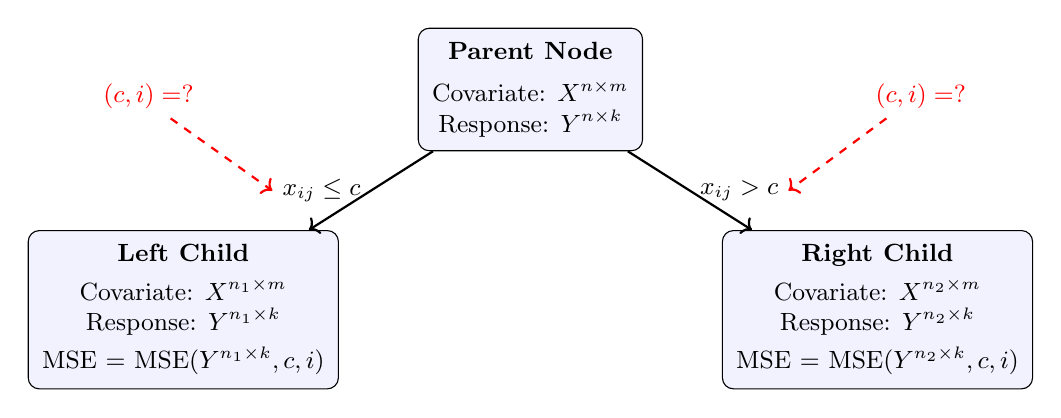
\begin{tikzpicture}[
  node distance=1cm and 1cm,
  every node/.style={font=\small},
  data/.style={rectangle, draw, align=center, fill=blue!5, rounded corners, inner sep=5pt},
  split/.style={->, thick},
  highlight/.style={->, red, thick, dashed}
  ]
  % Parent node
  \node[data] (parent) {
    \textbf{Parent Node} \\[0.15cm]
    Covariate: $X^{n \times m}$ \\ 
    Response: $Y^{n \times k}$
  };
  % Left child
  \node[data, below left=of parent] (left) {
    \textbf{Left Child} \\[0.1cm]
    Covariate: $X^{n_1 \times m}$ \\
    Response: $Y^{n_1 \times k}$ \\[0.1cm]
    MSE = $\text{MSE}(Y^{n_1 \times k},c,i)$
  };
  % Right child
  \node[data, below right=of parent] (right) {
    \textbf{Right Child} \\[0.1cm]
    Covariate: $X^{n_2 \times m}$ \\
    Response: $Y^{n_2 \times k}$ \\[0.1cm]
    MSE = $\text{MSE}(Y^{n_2 \times k},c,i)$
  };
  % Arrows
  \draw[split] (parent) -- node[midway, left] (leftlabel) {$x_{ij} \leq c$} (left);
  \draw[split] (parent) -- node[midway, right] (rightlabel) {$x_{ij} > c$} (right);
  
  % Optimize labels
  \node[red, left] (opt_i) at ([xshift=-1.5cm, yshift=1.2cm]leftlabel) {\textbf{ } $(c,i)=?$};
  \node[red, right] (opt_c) at ([xshift=1.5cm, yshift=1.2cm]rightlabel) {\textbf{} $(c,i)=?$};
  
  % Short highlight arrows from labels to split conditions
  \draw[highlight] (opt_i) -- (leftlabel.west);
  \draw[highlight] (opt_c) -- (rightlabel.east);
\end{tikzpicture}

\begin{align*}
    
(c^*, i^*) 
&=& \operatorname{argmin}_{i,c} \left( \text{MSE}(Y^{n_1 \times k},c,i) + \text{MSE}(Y^{n_2 \times k},c,i) \right)
\\
&=& \arg\min_{c,j} 
\left\{\frac{n_1(c,j)}{n}
\sum_{m=1}^k \sum_{i=1}^{n_1(c,j)} (y_{im}-\bar{y}_{m}^{n_1(c,j)})^2
+
\frac{n_2(c,j)}{n}
\sum_{m=1}^k \sum_{i=1}^{n_2(c,j)} (y_{im}-\bar{y}_{m}^{n_2(c,j)})^2
\right\}.
\end{align*}

}



\only<2>{ \frametitle{MSE splitting}

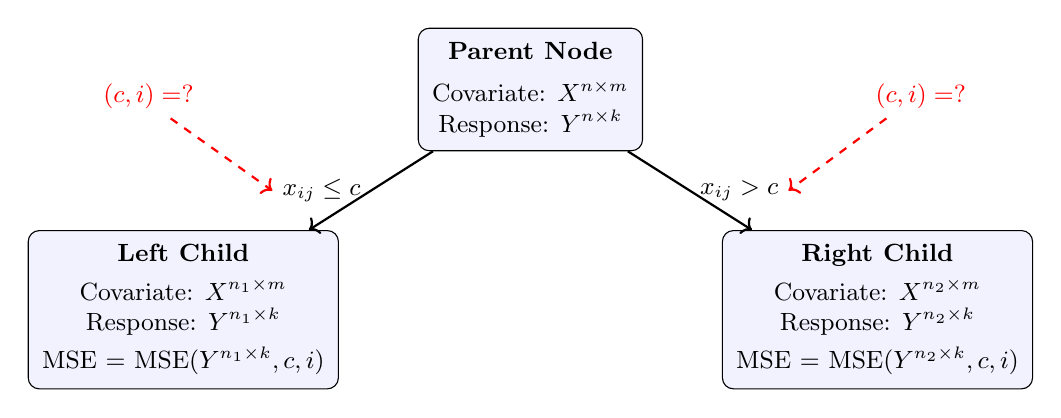
\begin{tikzpicture}[
  node distance=1cm and 1cm,
  every node/.style={font=\small},
  data/.style={rectangle, draw, align=center, fill=blue!5, rounded corners, inner sep=5pt},
  split/.style={->, thick},
  highlight/.style={->, red, thick, dashed}
  ]
  % Parent node
  \node[data] (parent) {
    \textbf{Parent Node} \\[0.15cm]
    Covariate: $X^{n \times m}$ \\ 
    Response: $Y^{n \times k}$
  };
  % Left child
  \node[data, below left=of parent] (left) {
    \textbf{Left Child} \\[0.1cm]
    Covariate: $X^{n_1 \times m}$ \\
    Response: $Y^{n_1 \times k}$ \\[0.1cm]
    MSE = $\text{MSE}(Y^{n_1 \times k},c,i)$
  };
  % Right child
  \node[data, below right=of parent] (right) {
    \textbf{Right Child} \\[0.1cm]
    Covariate: $X^{n_2 \times m}$ \\
    Response: $Y^{n_2 \times k}$ \\[0.1cm]
    MSE = $\text{MSE}(Y^{n_2 \times k},c,i)$
  };
  % Arrows
  \draw[split] (parent) -- node[midway, left] (leftlabel) {$x_{ij} \leq c$} (left);
  \draw[split] (parent) -- node[midway, right] (rightlabel) {$x_{ij} > c$} (right);
  
  % Optimize labels
  \node[red, left] (opt_i) at ([xshift=-1.5cm, yshift=1.2cm]leftlabel) {\textbf{ } $(c,i)=?$};
  \node[red, right] (opt_c) at ([xshift=1.5cm, yshift=1.2cm]rightlabel) {\textbf{} $(c,i)=?$};
  
  % Short highlight arrows from labels to split conditions
  \draw[highlight] (opt_i) -- (leftlabel.west);
  \draw[highlight] (opt_c) -- (rightlabel.east);
\end{tikzpicture}
\begin{itemize}
    \item 
MSE does not account for the simplex constraint.

\item 
\[V(X_i)=\frac{E(X_i)\left(1-E(X_i)\right)}{\alpha_0+1}\]
\end{itemize}

}

\end{frame}







\begin{frame}
\only<1>{
\frametitle{Dirichlet distribution}


\vspace{1em}

\begin{center}
\colorbox{green!10}{\parbox{0.95\textwidth}{
\begin{center}
\resizebox{\linewidth}{!}{%
\[
    f_{\mathbf{Z}}((z_1,\ldots,z_k); \boldsymbol{\alpha}) = \frac{\Gamma( \alpha_0)}{\prod_{i=1}^k \Gamma(\alpha_i)} \prod_{i=1}^k z_i^{\alpha_i - 1},
\quad  z_i \in [0, 1], \quad \sum_{i=1}^k z_i = 1,
\]
}
\end{center}
}}
\end{center}

\vspace{1.5em}

\begin{itemize}[itemsep=0.8em]


\item[\textcolor{blue}{\large$\blacktriangleright$}] The sum-constant requirement of the simplex is satisfied under the Dirichlet distribution.

\item[\textcolor{blue}{\large$\blacktriangleright$}] \textbf{Extensions available:} Zero-inflated Dirichlet and Kummer–Dirichlet
\end{itemize}
}

\end{frame}


\begin{frame}
\only<1>{\frametitle{Dirichlet log-likelihood splitting}

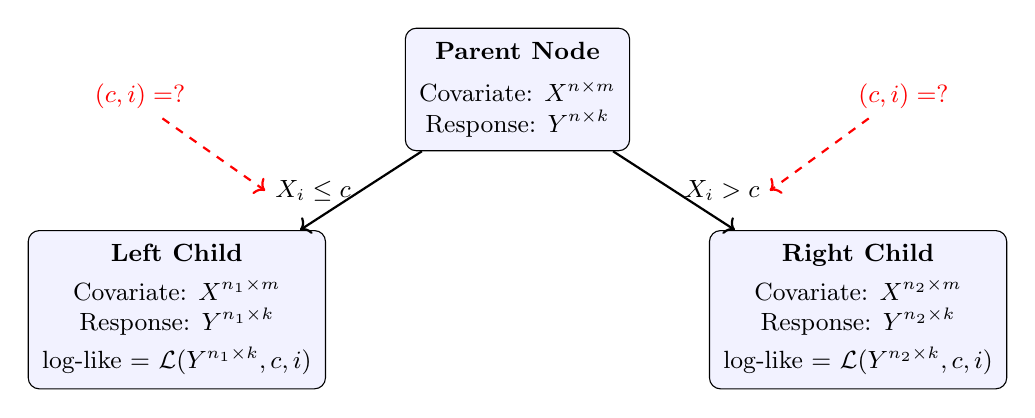
\begin{tikzpicture}[
  node distance=1cm and 1cm,
  every node/.style={font=\small},
  data/.style={rectangle, draw, align=center, fill=blue!5, rounded corners, inner sep=5pt},
  split/.style={->, thick},
  highlight/.style={->, red, thick, dashed}
  ]
  % Parent node
  \node[data] (parent) {
    \textbf{Parent Node} \\[0.15cm]
    Covariate: $X^{n \times m}$ \\ 
    Response: $Y^{n \times k}$
  };
  % Left child
  \node[data, below left=of parent] (left) {
    \textbf{Left Child} \\[0.1cm]
    Covariate: $X^{n_1 \times m}$ \\
    Response: $Y^{n_1 \times k}$ \\[0.1cm]
     log-like = $\mathcal{L}(Y^{n_1 \times k},c,i)$
  };
  % Right child
  \node[data, below right=of parent] (right) {
    \textbf{Right Child} \\[0.1cm]
    Covariate: $X^{n_2 \times m}$ \\
    Response: $Y^{n_2 \times k}$ \\[0.1cm]
     log-like = $\mathcal{L}(Y^{n_2 \times k},c,i)$
  };
  % Arrows
  \draw[split] (parent) -- node[midway, left] (leftlabel) {$X_{i} \leq c$} (left);
  \draw[split] (parent) -- node[midway, right] (rightlabel) {$X_{i} > c$} (right);
  
  % Optimize labels
  \node[red, left] (opt_i) at ([xshift=-1.5cm, yshift=1.2cm]leftlabel) {\textbf{ } $(c,i)=?$};
  \node[red, right] (opt_c) at ([xshift=1.5cm, yshift=1.2cm]rightlabel) {\textbf{} $(c,i)=?$};
  
  % Short highlight arrows from labels to split conditions
  \draw[highlight] (opt_i) -- (leftlabel.west);
  \draw[highlight] (opt_c) -- (rightlabel.east);
\end{tikzpicture}
\[
(c^*, i^*) = \operatorname{argmax}_{i,c} \left( \max_{\boldsymbol{\alpha}} \mathcal{L}(Y^{n_1 \times k},c,i) + \max_{\boldsymbol{\alpha}} \mathcal{L}(Y^{n_2 \times k},c,i) \right)
\]
}
\end{frame}

\begin{frame}{Prediction based on DirichletRF}

    
\begin{columns}[T]

% Left column - Graph
\begin{column}{0.45\textwidth}
\centering
\begin{tikzpicture}[
    node/.style={ellipse, draw, minimum width=1.2cm, minimum height=0.8cm, thick},
    leaf/.style={rectangle, draw, minimum width=1.8cm, minimum height=0.6cm, thick},
    arrow/.style={->, thick, blue},
    scale=0.75,
    every node/.style={transform shape}
]

% Root node
\node[node] (root) at (0,0) {};

% Level 1
\node[node] (n1) at (-2,-2) {};
\node (dots1) at (1,-2) {\vdots};

% Level 2
\node (dots2) at (-3,-3.5) {\vdots};
\node[node] (n2) at (-1,-4) {};

% Level 3
\node (dots3) at (-2.5,-5.5) {\vdots};
\node[node] (n3) at (0,-6) {};

% Level 4
\node (dots4) at (1,-7.5) {\vdots};
\node[leaf] (leaf) at (-1,-8) {$\{y_1, y_2, \ldots, y_{n_t^'}\}$};

% Arrows - traversal path highlighted
\draw[arrow, line width=1.5pt] (root) -- (n1);
\draw[arrow, dashed] (root) -- (dots1);
\draw[arrow, dashed] (n1) -- (dots2);
\draw[arrow, line width=1.5pt] (n1) -- (n2);
\draw[arrow, dashed] (n2) -- (dots3);
\draw[arrow, line width=1.5pt] (n2) -- (n3);
\draw[arrow, line width=1.5pt] (n3) -- (leaf);
\draw[arrow, dashed] (n3) -- (dots4);

\end{tikzpicture}
\end{column}

% Right column - Explanation
\begin{column}{0.52\textwidth}
\small

\textbf{Process:}
\begin{itemize}
\item[1)] Start at root node
    \item[2)] Traverse tree based on decision rules
    \item[3)] Reach terminal node with observations
\end{itemize}

\vspace{0.4cm}

\textbf{Default Approach:}
\begin{itemize}
    \item Mean: $\hat{y} = \frac{1}{n_t^'}\sum_{i=1}^{n_t^{'}} y_i$
    \item Expectation: $\text{E}(Y_i) = \frac{\hat{\alpha}_i}{\sum_{j+1}^k\hat{\alpha}_i}$
    \item Random Forest: average across trees
\end{itemize}

\vspace{0.4cm}

\textbf{Distributional Approach:}
\begin{itemize}
    \item Collect terminal nodes from all trees
    \item Construct empirical probability function
\end{itemize}

\end{column}

\end{columns}

\end{frame}










%-----------------------------------------------------------------------------
%===================================================
% Comparison Results


\begin{frame}{Comparison Results}
      \centering
      \vfill
      \textbf{\Large Comparison Results}
      \vfill
\end{frame}

\begin{frame}{Performance Evaluation and Transformations}

To evaluate DirichletRF's performance, we compare it with two alternative approaches:
\begin{itemize}
    \item[1)] \textbf{ILR-RF:} A Random Forest model based on log-ratio transformations. 
    The compositional data are first transformed into the ILR
    space. Then, a standard Random Forest is applied to the transformed data, and 
    finally, the predictions are mapped back to the simplex for interpretation.

    \item[2)] \textbf{Dirichlet Regression:} A parametric approach that, 
    works directly on the simplex without requiring any transformation.
\end{itemize}

\end{frame}




\begin{frame}{Evaluation Metrics}

To compare these models, we used  the Aitchison Distance.
\vspace{0.2cm}
\[
AC = \frac{1}{n} \sum_{i=1}^n \sqrt{\sum_{j=1}^k \left(\log\frac{Y_{ij}}{g(\mathbf{Y}_i)} - \log\frac{\hat{Y}_{ij}}{g(\hat{\mathbf{Y}}_i)}\right)^2},
\]
\[
\text{where} \quad g(\mathbf{Y}_i) = \left(\prod_{j=1}^k Y_{ij}\right)^{1/k}
\]


\vspace{0.3cm}
\textbf{Interpretation:} Lower values for this metric indicate better predictive accuracy.
\end{frame}








\begin{frame}{}

    \only<1>{
  
    \textbf{Simple structure simulations}: We use a simple dataset with $3$ Covariate variables, $X_1,X_1, X_{3}$ and with a $3$-dimensional response, $(Y_1,\,Y_2,\,Y_3)$ such that $Y_1+Y_2+Y_3 = 1$. The response is assumed to follow a Dirichlet distribution with the following parameters:
\[
\alpha_1 = 1 + 2 X_1,\quad \alpha_2 =1 + 0.5 X_2,\quad \alpha_3 = 1 + X_3.
\]
\[
(Y_1,\,Y_2,\,Y_3)\sim Dirichlet(\alpha_1,\alpha_2,\alpha_3)
\]
    }
    \only<2>{
      
Dirichlet Regression performed better than the other models. This result makes sense, because the data was generated using a Dirichlet distribution with a linear structure.


But, Dirichlet Random Forest does not perform well in this case — in fact, it gives the worst performance in terms of Aitchison Distance and RMSE.
\begin{table}[htbp]
\centering
\small 
\begin{tabular}{|l|l|c|c|}
\hline
$N$ & Model & Aitchison Distance & Train-Test \\
\hline
\multirow{3}{*}{200} 
    & ILR-RF & 1.303 (0.143) & 0.686 \\
    & \textcolor{blue}{Dirichlet Regression} & \textcolor{blue}{\textbf{1.233} (0.139)} & \textcolor{blue}{\textbf{0.030}} \\
    & \texttt{Dirichlet-RF} & 1.451 (0.153) & 0.600 \\
\hline
\multirow{3}{*}{500}
    & ILR-RF & 1.284 (0.077) & 0.685 \\
    & \textcolor{blue}{Dirichlet Regression} & \textcolor{blue}{\textbf{1.234} (0.078)} & \textcolor{blue}{\textbf{0.035}} \\
    & \texttt{Dirichlet-RF} & 1.450 (0.077) & 0.616 \\
\hline
\multirow{3}{*}{2000}
    & ILR-RF & 1.252 (0.032) & 0.654 \\
    & \textcolor{blue}{Dirichlet Regression} & \textcolor{blue}{\textbf{1.209} (0.032)} & \textcolor{blue}{\textbf{0.006}} \\
    & \texttt{Dirichlet-RF} & 1.431 (0.041) & 0.596 \\
\hline
\end{tabular}
\caption{Values represent the means and (standard deviations) of the metrics for test datasets. Train-Test Diff represents the absolute difference between train and test Aitchison Distance, indicating model generalisation capability.}
\label{tab:performance-comparison1}
\end{table}}

    \only<3>{
    	    

    
    Complex structure synthetic simulations: The dataset consisted of 10 predictor variables \((X_1, \ldots, X_{10})\), with only the first three variables \((X_1, X_2, X_3)\) being truly informative for predicting the compositional response. The three-component compositional response vector $\mathbf{Y} = (Y_1,Y_2,Y_3)$ was constructed through complex non-linear transformations of the informative Covariates. }
    \end{frame}
\begin{frame}
    \only<1>{

\begin{columns}
\begin{column}{0.5\linewidth}

% where \( \mathcal{N}(\mu_i, 0.5^2) \) represents a normally distributed random variable with mean \( \mu_i \) and standard deviation \( 0.5 \), and \( \epsilon \) is a small positive constant ensuring non-negativity.  
% The compositional response variables \( Y_1, Y_2, Y_3 \) are then obtained via the normalisation:
We generate the variables \( Z_1, Z_2, Z_3 \) as follows:  
\[
Z_i = \max(\epsilon, \mathcal{N}(\mu_i, 0.5)), \quad 
\]
\[
Y_i = \frac{Z_i}{Z_1 + Z_2 + Z_3}, \quad  i = 1,2,3.
\]
% This transformation ensures that \( (Y_1, Y_2, Y_3) \) lies within the unit simplex, preserving the compositional structure of the data.
\end{column}
		\begin{column}{0.5\linewidth}

\begin{align*}
\mu_{1j} &= g(2(1 + \sin(x_{1j}))+x_{2j}^3) \\
\mu_{2j} &= g(1 + 2.5\exp(x_{3j})+x_{1j}^2) \\
\mu_{3j} &= g(1 + (1+x_{2j})^2+x_{3j}^4)
\end{align*}

\end{column}

\end{columns}

Where
\[
g(x_{ij}) =
\begin{cases} 
    2, & x_{ij} < \text{Quantile}(x_i, 0.3) \\
    3, & \text{Quantile}(x_i, 0.3) \leq x_{ij} <\text{Quantile}(x_i, 0.6) \\
    4, & \text{Quantile}(x, 0.6) \leq x_{ij} \leq \text{Quantile}(x_i, 0.8) \\
    1, & x_i > \text{Quantile}(x_i, 0.8)
\end{cases}
\]

}
\end{frame}
\begin{frame}
\only<1>{

In this complex scenario, the results are reversed. Our Dirichlet-RF is now the best model, and Dirichlet Regression is the worst.
\begin{table}[htbp]
\centering
\small 
\begin{tabular}{|l|l|c|c|}
\hline
$N$ & Model & Aitchison Distance & Train-Test \\
\hline
\multirow{3}{*}{200} 
    & ILR-RF & 0.670 (0.151) & 0.364 \\
    & Dirichlet Regression & 0.826 (0.155) & 0.068 \\
    & \textcolor{blue}{\texttt{Dirichlet-RF}} & \textcolor{blue}{\textbf{0.659} (0.152)} & \textcolor{blue}{0.221} \\
\hline
\multirow{3}{*}{500}
    & ILR-RF & 0.618 (0.072) & 0.334 \\
    & Dirichlet Regression & 0.790 (0.075) & 0.029 \\
    & \textcolor{blue}{\texttt{Dirichlet-RF}} & \textcolor{blue}{\textbf{0.606} (0.068)} & \textcolor{blue}{0.201} \\
\hline
\multirow{3}{*}{2000}
    & ILR-RF & 0.557 (0.044) & 0.301 \\
    & Dirichlet Regression & 0.785 (0.044) & 0.016 \\
    & \textcolor{blue}{\texttt{Dirichlet-RF}} & \textcolor{blue}{\textbf{0.544} (0.044)} & \textcolor{blue}{0.178} \\
\hline
\end{tabular}
\caption{Train-Test Diff represents the absolute difference between train and test Aitchison Distance.}
\label{tab:performance-comparison}
\end{table}
}
\end{frame}



\begin{frame}{Learning Curve}
\only<1>{


\begin{figure}
    \centering
    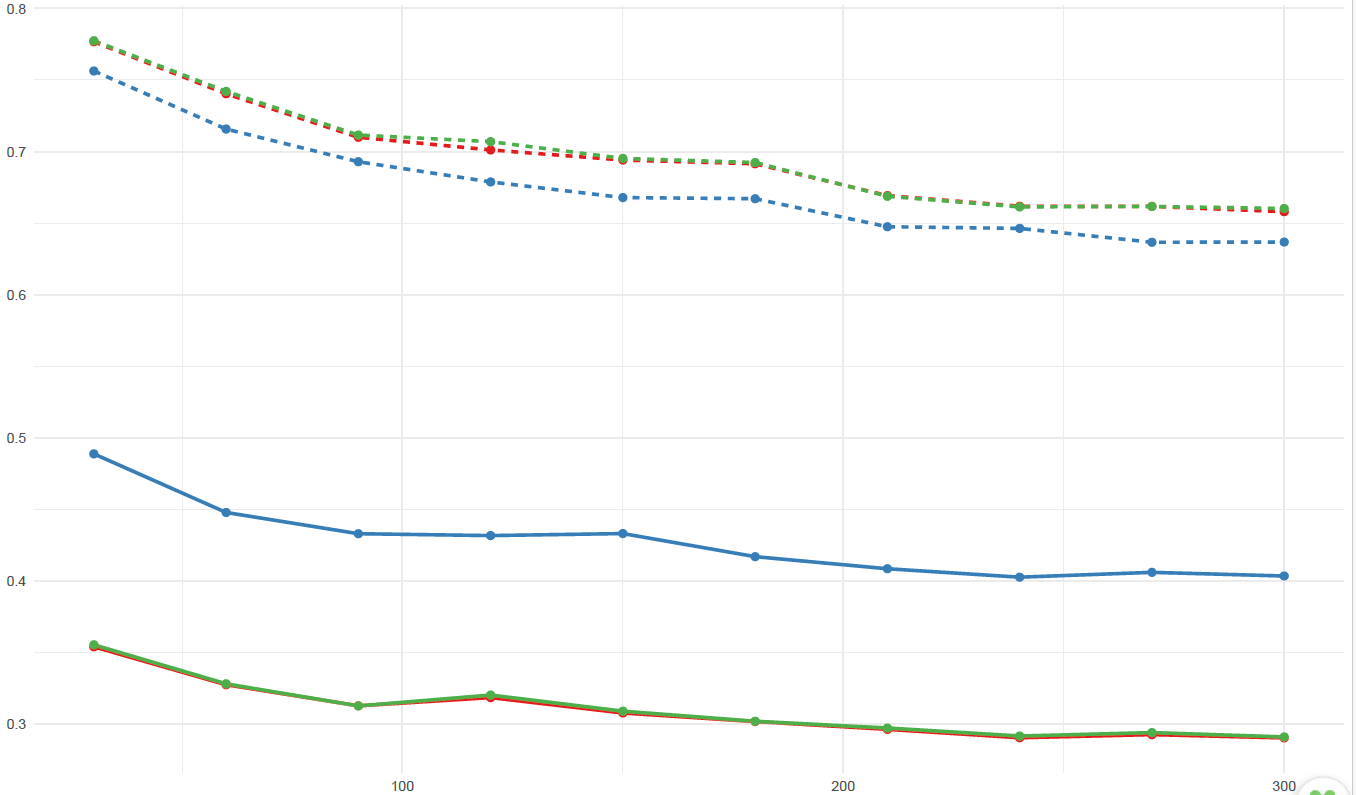
\includegraphics[width=0.75\linewidth]{Learning_curve.png}
    \caption{Aitchison distance as a function of training sample size for all three 
    Random Forest models.}
    \label{fig:enter-label}
\end{figure}
}
\end{frame}




% \begin{frame}
% \only<1>{
% \note{I am not sure to include this slide:

% And for further evaluation of \texttt{Dirichlet-RF}, we also looked at its performance in terms of covariate selection.

% Here, you can see how often each covariate was selected for splitting across all trees, and how much, on average, it contributed to increasing the log-likelihood.

% As I mentioned earlier, only three of the variables were informative — and \texttt{Dirichlet-RF} was able to clearly identify them with high importance.}
% \begin{table}[htbp]
% \centering
% \begin{tabular}{|c|c|c|}
% \hline
% \textbf{Covariate} & \small{Log-Likelihood Importance} & \small{Frequency-Based Importance} \\
% \hline
% \textcolor{blue}{$X_1$} & \textcolor{blue}{225.039} & \textcolor{blue}{14} \\
% \textcolor{blue}{$X_2$} & \textcolor{blue}{303.618} & \textcolor{blue}{21} \\
% \textcolor{blue}{$X_3$} & \textcolor{blue}{272.036} & \textcolor{blue}{19} \\
% \textcolor{red}{$X_4$} & \textcolor{red}{16.839}  & \textcolor{red}{2}  \\
% \textcolor{red}{$X_5$} & \textcolor{red}{9.972}   & \textcolor{red}{2}  \\
% \textcolor{red}{$X_6$} & \textcolor{red}{15.649}  & \textcolor{red}{3}  \\
% \textcolor{red}{$X_7$} & \textcolor{red}{0}   & \textcolor{red}{0}  \\
% \textcolor{red}{$X_8$} & \textcolor{red}{40.240}  & \textcolor{red}{6}  \\
% \textcolor{red}{$X_9$} & \textcolor{red}{5.369}   & \textcolor{red}{1}  \\
% \textcolor{red}{$X_{10}$} & \textcolor{red}{23.295}  & \textcolor{red}{3}  \\
% \hline
% \end{tabular}
% \caption{Variable importance scores based on log-likelihood improvement and selection frequency, averaged across all trees in the \texttt{Dirichlet-RF}.}

% \label{tab:variable-importance}
% \end{table}

% }
% \end{frame}






\begin{frame}{Implementation \& Code Access}
\note{This model was developed in Julia, and the full code is available on GitHub at the link provided.

We chose Julia mainly because of its strong computational performance. Implementing the model directly in R or Python would be much slower.

However, if you're working in R or Python, you can still use the model by calling the Julia functions from those languages.
We've included clear instructions in the repository, especially on how to connect Julia with R.

We're also planning to develop an R package with a C++ backend, which we hope to submit to CRAN, so the model will be even easier for R users to access.}
\vspace{1em}

\begin{itemize}[itemsep=1em]
\item[\textcolor{blue}{\large$\blacktriangleright$}] Model developed in \textbf{Julia} for computational efficiency

\item[\textcolor{blue}{\large$\blacktriangleright$}] Code available on \href{https://github.com/Xaleed/DirichletRandomForestJulia.git}{\textcolor{blue}{\textbf{GitHub}}}:

\textcolor{blue}{\small{https://github.com/Xaleed/DirichletRandomForestJulia.git}}
  \begin{center}

    \qrcode{https://github.com/Xaleed/DirichletRandomForestJulia.git}
 \end{center}



\end{itemize}

\vspace{1.5em}

\end{frame}


\begin{frame}{Alternative to MLE}
    \only<1>{
    \begin{block}{}
        One simple way to address this issue is to use the method of moments (MoM) as an alternative to maximum likelihood estimation (MLE). MoM gives an approximate solution but is much faster to compute.
    \end{block}
     \begin{block}{}
        We can also combine both approaches — instead of using MoM in all nodes, we can selectively apply it only in nodes where we expect its results to be close to MLE. This helps reduce computation while still keeping good accuracy.
    \end{block}
            \resizebox{0.65\linewidth}{!}{%

\begin{table}[htbp]
\centering

\begin{tabular}{|l|c|c|c|c|}
\hline
\multirow{2}{*}{Metric} & \multicolumn{2}{c|}{MLE} & \multicolumn{2}{c|}{MoM} \\
\cline{2-5}
 & (Train) & (Test) & (Train) & (Test) \\
\hline
Aitchison Distance & 0.3901 & 0.7391 & 0.4068 & 0.7457 \\
\hline
\end{tabular}
\end{table}}



}
\end{frame}



% \begin{frame}[plain]
% % \begin{center}
% %    
\includegraphics[width=5cm]{logo.png} % Optional logo
% %    \end{center}
%   \begin{center}
%       \vspace{2cm}

%     {\Huge \textbf{Thank You!} \par}
%     % \vspace{1cm}
%     % {\Large Questions or Comments? \par}
%     \vspace{1cm}
   
    
%     \qrcode{https://github.com/Xaleed/DirichletRandomForestJulia.git}
%    % \texttt{khaledmasoumifard@sun.ac.za}
%   \end{center}
% \end{frame}






% \end{document}










% % Auriga theme
% % find the most up-to-date version here: https://github.com/anishathalye/auriga

% \documentclass[aspectratio=169]{beamer}

% % ── Fonts & Encoding ──────────────────────────────────────────────
% \usepackage[T1]{fontenc}
% \usepackage{lmodern}

% % ── Math ──────────────────────────────────────────────────────────
% \usepackage{amsmath}
% \usepackage{amssymb}

% % ── Graphics & Color ──────────────────────────────────────────────
% \usepackage{graphicx}
% \usepackage{xcolor}
% \usepackage{colortbl}
% \usepackage{tcolorbox}

% % ── TikZ ──────────────────────────────────────────────────────────
% \usepackage{tikz}
% \usetikzlibrary{arrows.meta, calc, decorations.pathreplacing, shapes, arrows, positioning}

% % ── Plots ─────────────────────────────────────────────────────────
% \usepackage{pgfplots}
% \pgfplotsset{compat=1.18}

% % ── Tables ────────────────────────────────────────────────────────
% \usepackage{booktabs}
% \usepackage{array}
% \usepackage{multirow}

% % ── Lists & Symbols ───────────────────────────────────────────────
% \usepackage{enumitem}
% \usepackage{pifont}

% % ── References & QR ───────────────────────────────────────────────
% \usepackage{natbib}   % for \citet, \citep
% \usepackage{qrcode}
% \usepackage{fancyvrb}
% \usepackage{pgfpages}

% % ── Theme ─────────────────────────────────────────────────────────
% \usetheme{auriga}
% \usecolortheme{auriga}

% % ── Custom Colors ─────────────────────────────────────────────────
% \definecolor{leftblue}{RGB}{219,234,254}
% \definecolor{rightred}{RGB}{254,226,226}
% \definecolor{mainblue}{RGB}{25,65,120}
% \definecolor{accentblue}{RGB}{65,130,195}
% \definecolor{lightgray}{RGB}{245,245,248}

% % \setbeamercolor{frametitle}{bg=mainblue, fg=white}
% % \setbeamercolor{title}{fg=white}
% % \setbeamercolor{block title}{bg=accentblue, fg=white}
% % \setbeamercolor{block body}{bg=lightgray}
% % \setbeamercolor{structure}{fg=mainblue}
% % \definecolor{simplexfill}{RGB}{127,119,221}
% % \definecolor{simplexedge}{RGB}{83,74,183}
% % \definecolor{pointcol}{RGB}{60,52,137}
% % \definecolor{axiscol}{RGB}{136,135,128}
% % \definecolor{gridfaint}{RGB}{180,178,169}

% %\ifnotes
% % \setbeamertemplate{note page}[plain]
% % \setbeameroption{show notes on second screen=right}
% %\fi

% %\setbeameroption{show notes}  % in preamble

% % % define some colors for a consistent theme across slides
% % \definecolor{red}{RGB}{181, 23, 0}
% % \definecolor{blue}{RGB}{0, 118, 186}
% % \definecolor{gray}{RGB}{146, 146, 146}

% % ── Title Info ────────────────────────────────────────────────────
% \title{Towards predictive modelling of compositional data}
% \author{
%   \underline{Khaled Masoumifard}\inst{1} \and
%   Stephan van der Westhuizen\inst{1} \and
%   Sugnet Gardner-Lubbe\inst{1}
% }
% \institute[shortinst]{
%   \inst{1} Dept.\ of Statistics and Actuarial Science,
%   Stellenbosch University, Stellenbosch, South Africa
%   % \samelineand \inst{2}  MuViSU(Centre for Multi-dimensional Data Visualisation), Stellenbosch University, Stellenbosch, South Africa
% }

% % ─────────────────────────────────────────────────────────────────
% \begin{document}
% 

  \setbeamercolor{page number in head/foot}{fg=background canvas.bg}
  \begin{frame}
    \begin{tikzpicture}[remember picture, overlay]
      \node[anchor=north west, xshift=1em, yshift=-1em] at (current page.north west) {
        
\includegraphics[width=3cm]{logo.png}
      };
    \end{tikzpicture}

    \titlepage


      \begin{center}
    %    
\includegraphics[width=0.15\linewidth]{slides/DirichletRF.jpg}
    \qrcode[height=2.8cm]{https://github.com/Xaleed/DirichletRF.git}

    \vspace{0.1cm}

    {\small GitHub repository}

  \end{center}
  \end{frame}



\begin{frame}{What is This Talk About?}
% \note{
% Good morning, and thank you for joining this talk. It is about developing DDRF, which is part of my postdoc project at Stellenbosch University, in collaboration with Stephan and Professor Lubbe.


% In a nutshell, I’ll shortly refer what composistional data is? I will explain why is it reasonable to develop a random forest model for composiational data?
% I will some comparison result?}

\vspace{2em}



\vspace{1.5em}

\begin{itemize}

  \item[\textcolor{blue}{\large$\blacktriangleright$}] \textbf{Compositional Data} -- Fundamental properties and modeling challenges
  \vspace{1em}

  \item[\textcolor{blue}{\large$\blacktriangleright$}] \textbf{Literature Review} -- Historical development and ongoing debates
  \vspace{1em}

  \item[\textcolor{blue}{\large$\blacktriangleright$}] \textbf{Machine Learning with Random Forests} -- Capturing complex relationships
  \vspace{1em}

  % \item[\textcolor{blue}{\large$\blacktriangleright$}] \textbf{Dirichlet Random Forest} -- Model formulation and motivation
  % \vspace{1em}

  \item[\textcolor{blue}{\large$\blacktriangleright$}] \textbf{Comparative Results} -- Assessing predictive performance
  \vspace{1em}

  \item[\textcolor{blue}{\large$\blacktriangleright$}] \textbf{DirichletRF R Package} -- Implementation and practical use

\end{itemize}

\vspace{2em}

\end{frame}


\begin{frame}{Compositional data}
\only<1>{


\vspace{1em}

A simplex is a convex space of all vectors with non-negative components that sum to a constant. 



\begin{center}
\colorbox{blue!10}{\parbox{0.8\textwidth}{
\begin{center}
\[
S^c_k = \left\{ (y_1, \dots, y_k)^\top \in \mathbb{R}^k \,\middle|\, y_i \geq 0, \ \sum_{i=1}^k y_i = \textcolor{blue}{c} \right\}
\]
\end{center}
}}
\end{center}



 It is common to set \(  \textcolor{blue}{c = 1} \). We refer to data from this space as \emph{compositional data}.
 

}



\only<2>{

\textbf{A practical view of compositional data}

\vspace{0.3cm}

Let $\mathbf{Y} = (Y_1, Y_2, \dots, Y_K)$ be a vector with positive components.

\vspace{0.3cm}

The compositional transformation is defined as:
\[
\mathbf{S} =
\left(
\frac{Y_1}{\sum_{i=1}^K Y_i}, \dots,
\frac{Y_K}{\sum_{i=1}^K Y_i}
\right)
\]

\vspace{0.3cm}

This vector lies in the simplex space.

\vspace{0.5cm}

However, in this transformation we lose information about the \textbf{absolute scale}, and we cannot uniquely recover the original vector.

But we preserve the \textbf{relative information}.
In particular, for any two components $i$ and $j$:
\[
\frac{Y_i}{Y_j} = \frac{S_i}{S_j}
\]





}

% \only<3>{
% \vspace{.2cm}
%    \textbf{Example}: consider 
% \(
% \mathbf{Y} = (2000, 3000, 5000),
% \)
% which represents the amount of money (in dollars) allocated to \textit{stocks}, \textit{bonds}, and \textit{cash} in an investment portfolio.  

% Then the following vector is a compositional data:
% \begin{align*}
% \scalebox{1.2}{$\left(\frac{2000}{2000+3000+5000},\;\frac{3000}{2000+3000+5000},\;\frac{5000}{2000+3000+5000}\right)$} = (0.2, 0.3, 0.5)
% \end{align*}

% \medskip

% Multiply by 100:
% \[
% 100 \cdot \mathbf{s}(\mathbf{Y}) = (20, 30, 50)
% \]

% \medskip

% Same proportions, different scale (percentages).
% \note{
% Here we see a portfolio allocation example.

% After normalization, we obtain proportions of total investment.

% Multiplying by 100 expresses them as percentages, which are more intuitive in finance.

% The relative allocation (20\%, 30\%, 50\%) remains unchanged regardless of the total invested amount.
% }
% }


\only<3>{


Consider a job application pool of $50$ applicants classified by academic background.
\vspace{0.3cm}

\begin{columns}
    \begin{column}{0.4\textwidth}
        \[
        \mathbf{Y} = (10, 15, 25)
        \]
    \end{column}
    \begin{column}{0.5\textwidth}
        \begin{tabular}{lr}
            Mathematics & 10 \\
            Statistics  & 15 \\
            Computer Science & 25 \\
        \end{tabular}
    \end{column}
\end{columns}

\vspace{0.3cm}
We normalize this vector to obtain a compositional representation:
\vspace{0.2cm}

\begin{columns}
    \begin{column}{0.5\textwidth}
        \[
        \mathbf{s}(\mathbf{Y}) = \left(\frac{10}{50}, \frac{15}{50}, \frac{25}{50}\right)
        \]
    \end{column}
    \begin{column}{0.4\textwidth}
        \[
        = (0.2, 0.3, 0.5)
        \]
        Interpreted as proportions.
    \end{column}
\end{columns}

\vspace{0.2cm}
Multiplying by $100$ gives percentages:
\vspace{0.2cm}

\begin{columns}
    \begin{column}{0.5\textwidth}
        \[
        100 \cdot \mathbf{s}(\mathbf{Y}) = (20\%, 30\%, 50\%)
        \]
    \end{column}
    \begin{column}{0.4\textwidth}
        \textbf{Key idea:} The information is identical — only the scale changes.
    \end{column}
\end{columns}


}

\end{frame}


% \begin{frame}{Statistical problems with compositional data}
% 1)spurouis corelation
% 2)The (sample) covariance matrix of the data is singular with rank equal to $D - 1$, since
% \[
% \sum_{i=1}^{D} \operatorname{cov}(y_1, y_i)
% = \operatorname{cov}\left(y_1, \sum_{i=1}^{D} y_i \right)
% = \operatorname{cov}(y_1, 1)
% = 0,
% \]
% or equivalently,
% \[
% \sum_{i=2}^{D} \operatorname{cov}(y_1, y_i)
% = -\operatorname{var}(y_1),
% \]
% where each $y_i$ is a component of the composition $\mathbf{y}$.
% 3) Evidently, the problems and issues associated
% with compositional data are too numerous to list here and this is beyond the scope of
% this review paper.

    
% \end{frame}

% \begin{frame}{What methodology is more approperiate?}
% Aitchison suugest to tranfer data...

% dicson had another idea...

% a long argue staeted between them ... and finally Aitchison used stupid word and dicson lift the discussion for evere...
% Aitchison keep continue work on his idea and bring a lot of attention this his idea so many researcher for a while tried to his idea ... 
% aclsy and .. belive this made bad effect on the the field ... and for a while many researcher tried to say you have to use transformation methods...

% They belived 
% \end{frame}




% =============================================================
%  SPURIOUS CORRELATION
%  % =============================================================
%  SPURIOUS CORRELATION
%  % =============================================================
%  SPURIOUS CORRELATION
%  \input{slides/Spurious_correlation}
% =============================================================


% ------------------------------------------------------------------
%  SLIDE 1 – Spurious Correlation (Pearson)
% ------------------------------------------------------------------

\begin{frame}{Correlation}
  \note{
Now, I extend this example to 500 different job opportunities.

In other words, I generated 500 similar datasets, although only a few rows are shown in this table. Each row represents the number of applicants for one job opportunity.

If we calculate the correlation between applicants with a Mathematics background and applicants with a Statistics background in the original count data, the result is close to zero, as you can see.

This is exactly what we expect, because the variables were generated independently.

Now, if we transform the same data into the simplex space, we obtain a very different result. The Mathematics and Statistics components become strongly negatively correlated.

So, what does this correlation actually mean? What kind of information can we extract from it?

This is not an easy question to answer.

A common mistake is to interpret this as an ordinary correlation between applicants from Mathematics and Statistics backgrounds, as we would do in a standard data table.

However, this interpretation is misleading.

These types of correlations are known as spurious correlations.

      }
\only<1>{
  \begin{columns}
    \column{0.5\textwidth}
    \textbf{Original Data (Counts)}

    \vspace{0.2cm}
    \begin{center}
    \begin{tabular}{ccc}
      \hline
      Math & Stats & CS \\
      \hline
      48  & 230 & 59  \\
      286 & 181 & 73  \\
      286 & 98  & 147 \\
      35  & 14  & 12  \\
      255 & 104 & 235 \\
      $\vdots$ & $\vdots$ & $\vdots$ \\
      \hline
    \end{tabular}
    \end{center}

    \vspace{0.2cm}
    \[
      \mathrm{corr}(\text{Math},\,\text{Stats}) = 0.087
    \]

    \column{0.5\textwidth}
    
  \end{columns}


}
\only<2>{
\begin{columns}
    \column{0.5\textwidth}
    \textbf{Original Data (Counts)}

    \vspace{0.2cm}
    \begin{center}
    \begin{tabular}{ccc}
      \hline
      Math & Stats & CS \\
      \hline
      48  & 230 & 59  \\
      286 & 181 & 73  \\
      286 & 98  & 147 \\
      35  & 14  & 12  \\
      255 & 104 & 235 \\
      $\vdots$ & $\vdots$ & $\vdots$ \\
      \hline
    \end{tabular}
    \end{center}

    \vspace{0.2cm}
    \[
      \mathrm{corr}(\text{Math},\,\text{Stats}) = 0.087
    \]

    \column{0.5\textwidth}
    \textbf{Compositional Data (Normalized to 100)}

    \vspace{0.2cm}
    \begin{center}
    \begin{tabular}{ccc}
      \hline
      Math & Stats & CS \\
      \hline
      14.2 & 68.2 & 17.5 \\
      53.0 & 33.5 & 13.5 \\
      53.9 & 18.5 & 27.7 \\
      57.4 & 23.0 & 19.7 \\
      42.9 & 17.5 & 39.6 \\
      $\vdots$ & $\vdots$ & $\vdots$ \\
      \hline
    \end{tabular}
    \end{center}

    \vspace{0.2cm}
    \[
      \mathrm{corr}(X_{\text{math}},\, X_{\text{stats}}) = -0.874
    \]
  \end{columns}

}

\end{frame}

\end{frame}
\begin{frame}{Spurious Correlation}

 


\only<1>{
\note{Remove this slide:
Spurious correlation

One important consequence of working with compositional data is spurious correlation.

This phenomenon was introduced by Pearson in 1897.

He showed that ratios that share a common denominator can appear correlated, even when the original variables are completely independent.

To see this, let us consider three independent random variables: A, B, and C.

Now suppose we construct two new variables by dividing A by C and B by C.

Even though A and B are independent, these two ratios can become correlated because they share the same denominator.

}
  \begin{block}{Pearson (1897)}
    Ratios that share a common denominator are correlated even when the
    original variables are \emph{completely independent}.
  \end{block}

  \vspace{0.4em}
  \textbf{Simple illustration:} Let $A$, $B$, $C$ be mutually independent. Then:
  \[
    \operatorname{corr}\!\left(\frac{A}{C},\;\frac{B}{C}\right) \neq 0
  \]
  \vspace{0.2em}
  The shared denominator $C$ couples the two ratios artificially.
  The observed correlation reflects the \textbf{denominator's variability},
  not any true relationship between $A$ and $B$.
}

\only<2>{
\note{Spurious correlation

One important consequence of working with compositional data is spurious correlation.

This phenomenon was introduced by Pearson in 1897.

He showed that ratios that share a common denominator can appear correlated, even when the original variables are completely independent.

To see this, let us consider three independent random variables: A, B, and C.

Now suppose we construct two new variables by dividing A by C and B by C.

Even though A and B are independent, these two ratios can become correlated because they share the same denominator.

We observe exactly the same phenomenon in compositional data.

Since all components are normalized by the same sum, a common dependency is introduced.

As a result, even if two components are independent in the original space, they may appear dependent in the simplex space.

However, this is not a mistake.

}
  \begin{block}{Pearson (1897)}
    Ratios that share a common denominator are correlated even when the
    original variables are \emph{completely independent}.
  \end{block}

  \vspace{0.4em}

  \begin{columns}[t]
    \begin{column}{0.38\textwidth}
      \textbf{Original vector:}\\[4pt]
      $\mathbf{Y} = (Y_1, Y_2, \ldots, Y_K) \in \mathbb{R}_+^K$
    \end{column}
    \begin{column}{0.58\textwidth}
      \textbf{Simplex (normalized):}\\[4pt]
      $\mathbf{s}(\mathbf{Y}) = \!\left(\dfrac{Y_1}{S},\, \dfrac{Y_2}{S},\, \ldots,\, \dfrac{Y_K}{S}\right),
      \quad S = \sum_{j=1}^{K} Y_j$
    \end{column}
  \end{columns}

  \vspace{0.5em}
  \rule{\textwidth}{0.3pt}
  \vspace{0.3em}

  Even if $\operatorname{corr}(Y_1,\, Y_2) = 0$, we usually observe:
  \[
    \boxed{\operatorname{corr}\!\left(\frac{Y_1}{S},\,\frac{Y_2}{S}\right) \neq 0}
  \]
}

\only<3>{
\note{Mathematically, everything is correct.

The problem is only interpretation.

Pearson’s warning was exactly about this point: we should not interpret correlations between ratios as correlations between the original variables.

Unfortunately, this mistake often happens in practice.

}
  \[
  \boxed{
    \operatorname{corr}\!\left(\frac{Y_1}{S}, \frac{Y_2}{S}\right)
    =
    \frac{
      \mathbb{E}\!\left(\frac{Y_1 Y_2}{S^2}\right)
      - \mathbb{E}\!\left(\frac{Y_1}{S}\right)\mathbb{E}\!\left(\frac{Y_2}{S}\right)
    }{
      \sqrt{\operatorname{Var}\!\left(\frac{Y_1}{S}\right)}\;
      \sqrt{\operatorname{Var}\!\left(\frac{Y_2}{S}\right)}
    }
  }
  \]
  \vspace{0.4em}
  \begin{block}{Pearson's warning}
    The danger arises when one interprets a correlation between ratios as evidence
    of a genuine association between the \emph{original} variables.
    Such an inference is \textbf{not justified} -- the correlation may exist
    entirely because of the shared denominator, with no signal from the data at all.
  \end{block}
}



\only<4>{
  \note{
  For example, consider a job application dataset with different academic backgrounds such as mathematics, statistics, and computer science.

In the original count data (On the left), the correlation between mathematics and statistics may be very small, close to zero.

However, after normalization to percentages — that is, after moving to the simplex space — the same variables can become strongly negatively or positively correlated.

      }

  \begin{columns}
    \column{0.5\textwidth}
    \textbf{Original Data (Counts)}

    \vspace{0.2cm}
    \begin{center}
    \begin{tabular}{ccc}
      \hline
      Math & Stats & CS \\
      \hline
      48  & 230 & 59  \\
      286 & 181 & 73  \\
      286 & 98  & 147 \\
      35  & 14  & 12  \\
      255 & 104 & 235 \\
      $\vdots$ & $\vdots$ & $\vdots$ \\
      \hline
    \end{tabular}
    \end{center}

    \vspace{0.2cm}
    \[
      \mathrm{corr}(\text{Math},\,\text{Stats}) = 0.087
    \]

    \column{0.5\textwidth}
    \textbf{Compositional Data (Normalized to 100)}

    \vspace{0.2cm}
    \begin{center}
    \begin{tabular}{ccc}
      \hline
      Math & Stats & CS \\
      \hline
      14.2 & 68.2 & 17.5 \\
      53.0 & 33.5 & 13.5 \\
      53.9 & 18.5 & 27.7 \\
      57.4 & 23.0 & 19.7 \\
      42.9 & 17.5 & 39.6 \\
      $\vdots$ & $\vdots$ & $\vdots$ \\
      \hline
    \end{tabular}
    \end{center}

    \vspace{0.2cm}
    \[
      \mathrm{corr}(X_{\text{math}},\, X_{\text{stats}}) = -0.874
    \]
  \end{columns}

  \vspace{0.3em}
  \textbf{Key message:} Spurious dependence:
  This correlation does \textbf{not} necessarily reflect a true relationship.
}

\end{frame}


% ------------------------------------------------------------------
%  SLIDE 2 – Statistical Difficulties: Singular Matrix
% ------------------------------------------------------------------
\begin{frame}{Statistical Difficulties}

\note{
Singularity of the covariance matrix

Another important consequence is that the covariance matrix is not invertible in the simplex space.

This can be shown quite easily.

Because of the constant-sum constraint, the components are not independent.

As a result, one degree of freedom is lost, and the covariance matrix becomes singular.

This creates a practical limitation.

Many standard statistical methods require the inverse of the covariance matrix, such as regression models and multivariate techniques.

Therefore, these methods cannot be directly applied to compositional data.

There are also several other difficulties that arise from working in the simplex space.

I will not go into all of them here.

However, all of these challenges motivated researchers to develop new methods specifically designed for compositional data.
}

\only<1>{
  \vspace{0.4em}
  \[
  \Sigma_{\mathbf{X}} =
  \begin{pmatrix}
    \operatorname{Var}(X_1)     & \operatorname{cov}(X_1,X_2) & \cdots & \operatorname{cov}(X_1,X_K) \\
    \operatorname{cov}(X_2,X_1) & \operatorname{Var}(X_2)     & \cdots & \operatorname{cov}(X_2,X_K) \\
    \vdots                      & \vdots                       & \ddots & \vdots \\
    \operatorname{cov}(X_K,X_1) & \operatorname{cov}(X_K,X_2) & \cdots & \operatorname{Var}(X_K)
  \end{pmatrix}
  \in \mathbb{R}^{K \times K}
  \]
  \vspace{0.2em}
  The \textbf{last row (and column) is linearly determined} by the others via the
  sum-to-constant constraint, confirming $\operatorname{rank}(\Sigma_{\mathbf{X}}) = K-1$.
}

\only<2>{
  The sum-to-constant constraint causes the \textbf{sample covariance matrix to be singular}:
  \[
    \sum_{i=1}^{K} \operatorname{cov}(X_1, X_i)
    = \operatorname{cov}\!\left(X_1,\, \sum_{i=1}^K X_i\right)
    = \operatorname{cov}(X_1,\, 1) = 0
  \]
  \[
    \Rightarrow\quad
    \sum_{i=2}^{K} \operatorname{cov}(X_1, X_i) = -\operatorname{Var}(X_1).
  \]

  \vspace{0.3em}
  $\Sigma_{\mathbf{X}}$ has rank $K-1$ $\;\Rightarrow\;$ \textbf{not invertible}.

  \vspace{0.5em}
  \begin{columns}[T]
    \begin{column}{0.48\textwidth}
      \textbf{Technical consequence:}
      \begin{itemize}
        \item Regression, LDA, and standard PCA all require $\Sigma^{-1}$ -- unavailable.
      \end{itemize}
    \end{column}
    \begin{column}{0.48\textwidth}
      \textbf{Conceptual consequence:}
      \begin{itemize}
        \item No universally accepted definition of correlation for compositional data exists yet.
      \end{itemize}
    \end{column}
  \end{columns}
}

\end{frame}


% ------------------------------------------------------------------
%  SLIDE 3 – The Log-Ratio Idea
% ------------------------------------------------------------------

% =============================================================


% ------------------------------------------------------------------
%  SLIDE 1 – Spurious Correlation (Pearson)
% ------------------------------------------------------------------

\begin{frame}{Correlation}
  \note{
Now, I extend this example to 500 different job opportunities.

In other words, I generated 500 similar datasets, although only a few rows are shown in this table. Each row represents the number of applicants for one job opportunity.

If we calculate the correlation between applicants with a Mathematics background and applicants with a Statistics background in the original count data, the result is close to zero, as you can see.

This is exactly what we expect, because the variables were generated independently.

Now, if we transform the same data into the simplex space, we obtain a very different result. The Mathematics and Statistics components become strongly negatively correlated.

So, what does this correlation actually mean? What kind of information can we extract from it?

This is not an easy question to answer.

A common mistake is to interpret this as an ordinary correlation between applicants from Mathematics and Statistics backgrounds, as we would do in a standard data table.

However, this interpretation is misleading.

These types of correlations are known as spurious correlations.

      }
\only<1>{
  \begin{columns}
    \column{0.5\textwidth}
    \textbf{Original Data (Counts)}

    \vspace{0.2cm}
    \begin{center}
    \begin{tabular}{ccc}
      \hline
      Math & Stats & CS \\
      \hline
      48  & 230 & 59  \\
      286 & 181 & 73  \\
      286 & 98  & 147 \\
      35  & 14  & 12  \\
      255 & 104 & 235 \\
      $\vdots$ & $\vdots$ & $\vdots$ \\
      \hline
    \end{tabular}
    \end{center}

    \vspace{0.2cm}
    \[
      \mathrm{corr}(\text{Math},\,\text{Stats}) = 0.087
    \]

    \column{0.5\textwidth}
    
  \end{columns}


}
\only<2>{
\begin{columns}
    \column{0.5\textwidth}
    \textbf{Original Data (Counts)}

    \vspace{0.2cm}
    \begin{center}
    \begin{tabular}{ccc}
      \hline
      Math & Stats & CS \\
      \hline
      48  & 230 & 59  \\
      286 & 181 & 73  \\
      286 & 98  & 147 \\
      35  & 14  & 12  \\
      255 & 104 & 235 \\
      $\vdots$ & $\vdots$ & $\vdots$ \\
      \hline
    \end{tabular}
    \end{center}

    \vspace{0.2cm}
    \[
      \mathrm{corr}(\text{Math},\,\text{Stats}) = 0.087
    \]

    \column{0.5\textwidth}
    \textbf{Compositional Data (Normalized to 100)}

    \vspace{0.2cm}
    \begin{center}
    \begin{tabular}{ccc}
      \hline
      Math & Stats & CS \\
      \hline
      14.2 & 68.2 & 17.5 \\
      53.0 & 33.5 & 13.5 \\
      53.9 & 18.5 & 27.7 \\
      57.4 & 23.0 & 19.7 \\
      42.9 & 17.5 & 39.6 \\
      $\vdots$ & $\vdots$ & $\vdots$ \\
      \hline
    \end{tabular}
    \end{center}

    \vspace{0.2cm}
    \[
      \mathrm{corr}(X_{\text{math}},\, X_{\text{stats}}) = -0.874
    \]
  \end{columns}

}

\end{frame}

\end{frame}
\begin{frame}{Spurious Correlation}

 


\only<1>{
\note{Remove this slide:
Spurious correlation

One important consequence of working with compositional data is spurious correlation.

This phenomenon was introduced by Pearson in 1897.

He showed that ratios that share a common denominator can appear correlated, even when the original variables are completely independent.

To see this, let us consider three independent random variables: A, B, and C.

Now suppose we construct two new variables by dividing A by C and B by C.

Even though A and B are independent, these two ratios can become correlated because they share the same denominator.

}
  \begin{block}{Pearson (1897)}
    Ratios that share a common denominator are correlated even when the
    original variables are \emph{completely independent}.
  \end{block}

  \vspace{0.4em}
  \textbf{Simple illustration:} Let $A$, $B$, $C$ be mutually independent. Then:
  \[
    \operatorname{corr}\!\left(\frac{A}{C},\;\frac{B}{C}\right) \neq 0
  \]
  \vspace{0.2em}
  The shared denominator $C$ couples the two ratios artificially.
  The observed correlation reflects the \textbf{denominator's variability},
  not any true relationship between $A$ and $B$.
}

\only<2>{
\note{Spurious correlation

One important consequence of working with compositional data is spurious correlation.

This phenomenon was introduced by Pearson in 1897.

He showed that ratios that share a common denominator can appear correlated, even when the original variables are completely independent.

To see this, let us consider three independent random variables: A, B, and C.

Now suppose we construct two new variables by dividing A by C and B by C.

Even though A and B are independent, these two ratios can become correlated because they share the same denominator.

We observe exactly the same phenomenon in compositional data.

Since all components are normalized by the same sum, a common dependency is introduced.

As a result, even if two components are independent in the original space, they may appear dependent in the simplex space.

However, this is not a mistake.

}
  \begin{block}{Pearson (1897)}
    Ratios that share a common denominator are correlated even when the
    original variables are \emph{completely independent}.
  \end{block}

  \vspace{0.4em}

  \begin{columns}[t]
    \begin{column}{0.38\textwidth}
      \textbf{Original vector:}\\[4pt]
      $\mathbf{Y} = (Y_1, Y_2, \ldots, Y_K) \in \mathbb{R}_+^K$
    \end{column}
    \begin{column}{0.58\textwidth}
      \textbf{Simplex (normalized):}\\[4pt]
      $\mathbf{s}(\mathbf{Y}) = \!\left(\dfrac{Y_1}{S},\, \dfrac{Y_2}{S},\, \ldots,\, \dfrac{Y_K}{S}\right),
      \quad S = \sum_{j=1}^{K} Y_j$
    \end{column}
  \end{columns}

  \vspace{0.5em}
  \rule{\textwidth}{0.3pt}
  \vspace{0.3em}

  Even if $\operatorname{corr}(Y_1,\, Y_2) = 0$, we usually observe:
  \[
    \boxed{\operatorname{corr}\!\left(\frac{Y_1}{S},\,\frac{Y_2}{S}\right) \neq 0}
  \]
}

\only<3>{
\note{Mathematically, everything is correct.

The problem is only interpretation.

Pearson’s warning was exactly about this point: we should not interpret correlations between ratios as correlations between the original variables.

Unfortunately, this mistake often happens in practice.

}
  \[
  \boxed{
    \operatorname{corr}\!\left(\frac{Y_1}{S}, \frac{Y_2}{S}\right)
    =
    \frac{
      \mathbb{E}\!\left(\frac{Y_1 Y_2}{S^2}\right)
      - \mathbb{E}\!\left(\frac{Y_1}{S}\right)\mathbb{E}\!\left(\frac{Y_2}{S}\right)
    }{
      \sqrt{\operatorname{Var}\!\left(\frac{Y_1}{S}\right)}\;
      \sqrt{\operatorname{Var}\!\left(\frac{Y_2}{S}\right)}
    }
  }
  \]
  \vspace{0.4em}
  \begin{block}{Pearson's warning}
    The danger arises when one interprets a correlation between ratios as evidence
    of a genuine association between the \emph{original} variables.
    Such an inference is \textbf{not justified} -- the correlation may exist
    entirely because of the shared denominator, with no signal from the data at all.
  \end{block}
}



\only<4>{
  \note{
  For example, consider a job application dataset with different academic backgrounds such as mathematics, statistics, and computer science.

In the original count data (On the left), the correlation between mathematics and statistics may be very small, close to zero.

However, after normalization to percentages — that is, after moving to the simplex space — the same variables can become strongly negatively or positively correlated.

      }

  \begin{columns}
    \column{0.5\textwidth}
    \textbf{Original Data (Counts)}

    \vspace{0.2cm}
    \begin{center}
    \begin{tabular}{ccc}
      \hline
      Math & Stats & CS \\
      \hline
      48  & 230 & 59  \\
      286 & 181 & 73  \\
      286 & 98  & 147 \\
      35  & 14  & 12  \\
      255 & 104 & 235 \\
      $\vdots$ & $\vdots$ & $\vdots$ \\
      \hline
    \end{tabular}
    \end{center}

    \vspace{0.2cm}
    \[
      \mathrm{corr}(\text{Math},\,\text{Stats}) = 0.087
    \]

    \column{0.5\textwidth}
    \textbf{Compositional Data (Normalized to 100)}

    \vspace{0.2cm}
    \begin{center}
    \begin{tabular}{ccc}
      \hline
      Math & Stats & CS \\
      \hline
      14.2 & 68.2 & 17.5 \\
      53.0 & 33.5 & 13.5 \\
      53.9 & 18.5 & 27.7 \\
      57.4 & 23.0 & 19.7 \\
      42.9 & 17.5 & 39.6 \\
      $\vdots$ & $\vdots$ & $\vdots$ \\
      \hline
    \end{tabular}
    \end{center}

    \vspace{0.2cm}
    \[
      \mathrm{corr}(X_{\text{math}},\, X_{\text{stats}}) = -0.874
    \]
  \end{columns}

  \vspace{0.3em}
  \textbf{Key message:} Spurious dependence:
  This correlation does \textbf{not} necessarily reflect a true relationship.
}

\end{frame}


% ------------------------------------------------------------------
%  SLIDE 2 – Statistical Difficulties: Singular Matrix
% ------------------------------------------------------------------
\begin{frame}{Statistical Difficulties}

\note{
Singularity of the covariance matrix

Another important consequence is that the covariance matrix is not invertible in the simplex space.

This can be shown quite easily.

Because of the constant-sum constraint, the components are not independent.

As a result, one degree of freedom is lost, and the covariance matrix becomes singular.

This creates a practical limitation.

Many standard statistical methods require the inverse of the covariance matrix, such as regression models and multivariate techniques.

Therefore, these methods cannot be directly applied to compositional data.

There are also several other difficulties that arise from working in the simplex space.

I will not go into all of them here.

However, all of these challenges motivated researchers to develop new methods specifically designed for compositional data.
}

\only<1>{
  \vspace{0.4em}
  \[
  \Sigma_{\mathbf{X}} =
  \begin{pmatrix}
    \operatorname{Var}(X_1)     & \operatorname{cov}(X_1,X_2) & \cdots & \operatorname{cov}(X_1,X_K) \\
    \operatorname{cov}(X_2,X_1) & \operatorname{Var}(X_2)     & \cdots & \operatorname{cov}(X_2,X_K) \\
    \vdots                      & \vdots                       & \ddots & \vdots \\
    \operatorname{cov}(X_K,X_1) & \operatorname{cov}(X_K,X_2) & \cdots & \operatorname{Var}(X_K)
  \end{pmatrix}
  \in \mathbb{R}^{K \times K}
  \]
  \vspace{0.2em}
  The \textbf{last row (and column) is linearly determined} by the others via the
  sum-to-constant constraint, confirming $\operatorname{rank}(\Sigma_{\mathbf{X}}) = K-1$.
}

\only<2>{
  The sum-to-constant constraint causes the \textbf{sample covariance matrix to be singular}:
  \[
    \sum_{i=1}^{K} \operatorname{cov}(X_1, X_i)
    = \operatorname{cov}\!\left(X_1,\, \sum_{i=1}^K X_i\right)
    = \operatorname{cov}(X_1,\, 1) = 0
  \]
  \[
    \Rightarrow\quad
    \sum_{i=2}^{K} \operatorname{cov}(X_1, X_i) = -\operatorname{Var}(X_1).
  \]

  \vspace{0.3em}
  $\Sigma_{\mathbf{X}}$ has rank $K-1$ $\;\Rightarrow\;$ \textbf{not invertible}.

  \vspace{0.5em}
  \begin{columns}[T]
    \begin{column}{0.48\textwidth}
      \textbf{Technical consequence:}
      \begin{itemize}
        \item Regression, LDA, and standard PCA all require $\Sigma^{-1}$ -- unavailable.
      \end{itemize}
    \end{column}
    \begin{column}{0.48\textwidth}
      \textbf{Conceptual consequence:}
      \begin{itemize}
        \item No universally accepted definition of correlation for compositional data exists yet.
      \end{itemize}
    \end{column}
  \end{columns}
}

\end{frame}


% ------------------------------------------------------------------
%  SLIDE 3 – The Log-Ratio Idea
% ------------------------------------------------------------------

% =============================================================


% ------------------------------------------------------------------
%  SLIDE 1 – Spurious Correlation (Pearson)
% ------------------------------------------------------------------

\begin{frame}{Correlation}

  
\only<1>{
  \begin{columns}
    \column{0.5\textwidth}
    \textbf{Original Data (Counts)}

    \vspace{0.2cm}
    \begin{center}
     \begin{tabular}{lccc}
      \hline
       & Math & Stats & CS \\
      \hline
      Job 1 & 48  & 230 & 59  \\
      Job 2 & 286 & 181 & 73  \\
      Job 3 & 286 & 98  & 147 \\
      Job 4 & 35  & 14  & 12  \\
      Job 5 & 255 & 104 & 235 \\
      $\vdots$ & $\vdots$ & $\vdots$ & $\vdots$ \\
      \hline
    \end{tabular}
    \end{center}

    \vspace{0.2cm}
    \[
      \mathrm{corr}(\text{Math},\,\text{Stats}) = 0.087
    \]

    \column{0.5\textwidth}
    
  \end{columns}


}
\only<2>{
\begin{columns}
    \column{0.5\textwidth}
    \textbf{Original Data (Counts)}
    \vspace{0.2cm}
    \begin{center}
    \begin{tabular}{lccc}
      \hline
       & Math & Stats & CS \\
      \hline
      Job 1 & 48  & 230 & 59  \\
      Job 2 & 286 & 181 & 73  \\
      Job 3 & 286 & 98  & 147 \\
      Job 4 & 35  & 14  & 12  \\
      Job 5 & 255 & 104 & 235 \\
      $\vdots$ & $\vdots$ & $\vdots$ & $\vdots$ \\
      \hline
    \end{tabular}
    \end{center}
    \vspace{0.2cm}
    \[
      \mathrm{corr}(\text{Math},\,\text{Stats}) = 0.087
    \]
    \column{0.5\textwidth}
    \textbf{Compositional Data (Normalized to 100)}
    \vspace{0.2cm}
    \begin{center}
    \begin{tabular}{lccc}
      \hline
       & Math & Stats & CS \\
      \hline
      Job 1 & 14.2 & 68.2 & 17.5 \\
      Job 2 & 53.0 & 33.5 & 13.5 \\
      Job 3 & 53.9 & 18.5 & 27.7 \\
      Job 4 & 57.4 & 23.0 & 19.7 \\
      Job 5 & 42.9 & 17.5 & 39.6 \\
      $\vdots$ & $\vdots$ & $\vdots$ & $\vdots$ \\
      \hline
    \end{tabular}
    \end{center}
    \vspace{0.2cm}
    \[
      \mathrm{corr}(X_{\text{math}},\, X_{\text{stats}}) = -0.874
    \]
  \end{columns}
   \vspace{0.1cm} 
What does $\mathrm{corr}(X_{\text{math}},\, X_{\text{stats}}) = -0.874$ mean? \vspace{0.1cm} 

\begin{alertblock}{Warning} A common mistake is to interpret this correlation as if it were computed on the raw counts. \end{alertblock}
}

\only<3>{
\begin{columns}
    \column{0.5\textwidth}
    \textbf{Original Data (Counts)}
    \vspace{0.2cm}
    \begin{center}
    \begin{tabular}{lccc}
      \hline
       & Math & Stats & CS \\
      \hline
      Job 1 & ?  & ? & ?  \\
      Job 2 & ? & ? & ?  \\
      Job 3 & ? & ?  & ? \\
      Job 4 & ?  & ?  & ?  \\
      Job 5 & ? & ? & ? \\
      $\vdots$ & $\vdots$ & $\vdots$ & $\vdots$ \\
      \hline
    \end{tabular}
    \end{center}
    \vspace{0.2cm}
    \[
      \mathrm{corr}(\text{Math},\,\text{Stats}) = \text{?}
    \]
    \column{0.5\textwidth}
    \textbf{Compositional Data (Normalized to 100)}
    \vspace{0.2cm}
    \begin{center}
    \begin{tabular}{lccc}
      \hline
       & Math & Stats & CS \\
      \hline
      Job 1 & 14.2 & 68.2 & 17.5 \\
      Job 2 & 53.0 & 33.5 & 13.5 \\
      Job 3 & 53.9 & 18.5 & 27.7 \\
      Job 4 & 57.4 & 23.0 & 19.7 \\
      Job 5 & 42.9 & 17.5 & 39.6 \\
      $\vdots$ & $\vdots$ & $\vdots$ & $\vdots$ \\
      \hline
    \end{tabular}
    \end{center}
    \vspace{0.2cm}
    \[
      \mathrm{corr}(X_{\text{math}},\, X_{\text{stats}}) = -0.874
    \]
  \end{columns}
  \vspace{0.1cm}
\begin{alertblock}{Warning}
In cases where only compositional data are observed, the original dependence structure is unknown and cannot be uniquely recovered from the simplex representation.\end{alertblock}
}

\end{frame}

\begin{frame}{Spurious Correlation}

 


% \only<1>{

%   \begin{block}{Pearson (1897)}
%     Ratios that share a common denominator are correlated even when the
%     original variables are \emph{completely independent}.
%   \end{block}

%   \vspace{0.4em}
%   \textbf{Simple illustration:} Let $A$, $B$, $C$ be mutually independent. Then:
%   \[
%     \operatorname{corr}\!\left(\frac{A}{C},\;\frac{B}{C}\right) \neq 0
%   \]
%   \vspace{0.2em}
%   The shared denominator $C$ couples the two ratios artificially.
%   The observed correlation reflects the \textbf{denominator's variability},
%   not any true relationship between $A$ and $B$.
% }

\only<1>{


  \begin{block}{Pearson (1897)}
    Ratios that share a common denominator are correlated even when the
    original variables are \emph{completely independent}.
  \end{block}

  \vspace{0.4em}

  \begin{columns}[t]
    \begin{column}{0.38\textwidth}
      \textbf{Original vector:}\\[4pt]
      $\mathbf{Y} = (Y_1, Y_2, \ldots, Y_K) \in \mathbb{R}_+^K$
    \end{column}
    \begin{column}{0.58\textwidth}
      \textbf{Simplex (normalized):}\\[4pt]
      $\mathbf{s}(\mathbf{Y}) = \!\left(\dfrac{Y_1}{S},\, \dfrac{Y_2}{S},\, \ldots,\, \dfrac{Y_K}{S}\right),
      \quad S = \sum_{j=1}^{K} Y_j$
    \end{column}
  \end{columns}

  \vspace{0.5em}
  \rule{\textwidth}{0.3pt}
  \vspace{0.3em}

  Even if $\operatorname{corr}(Y_1,\, Y_2) = 0$, we usually observe:
  \[
    \boxed{\operatorname{corr}\!\left(\frac{Y_1}{S},\,\frac{Y_2}{S}\right) \neq 0}
  \]
}

% \only<3>{

%   \[
%   \boxed{
%     \operatorname{corr}\!\left(\frac{Y_1}{S}, \frac{Y_2}{S}\right)
%     =
%     \frac{
%       \mathbb{E}\!\left(\frac{Y_1 Y_2}{S^2}\right)
%       - \mathbb{E}\!\left(\frac{Y_1}{S}\right)\mathbb{E}\!\left(\frac{Y_2}{S}\right)
%     }{
%       \sqrt{\operatorname{Var}\!\left(\frac{Y_1}{S}\right)}\;
%       \sqrt{\operatorname{Var}\!\left(\frac{Y_2}{S}\right)}
%     }
%   }
%   \]
%   \vspace{0.4em}
%   \begin{block}{Pearson's warning}
%     The danger arises when one interprets a correlation between ratios as evidence
%     of a genuine association between the \emph{original} variables.
%     Such an inference is \textbf{not justified} -- the correlation may exist
%     entirely because of the shared denominator, with no signal from the data at all.
%   \end{block}
% }




\end{frame}


% ------------------------------------------------------------------
%  SLIDE 2 – Statistical Difficulties: Singular Matrix
% ------------------------------------------------------------------
\begin{frame}{Statistical Difficulties}



\only<1>{
  \vspace{0.4em}
  \[
  \Sigma_{\mathbf{X}} =
  \begin{pmatrix}
    \operatorname{Var}(X_1)     & \operatorname{cov}(X_1,X_2) & \cdots & \operatorname{cov}(X_1,X_K) \\
    \operatorname{cov}(X_2,X_1) & \operatorname{Var}(X_2)     & \cdots & \operatorname{cov}(X_2,X_K) \\
    \vdots                      & \vdots                       & \ddots & \vdots \\
    \operatorname{cov}(X_K,X_1) & \operatorname{cov}(X_K,X_2) & \cdots & \operatorname{Var}(X_K)
  \end{pmatrix}
  \in \mathbb{R}^{K \times K}
  \]
  \vspace{0.2em}
  The \textbf{last row (and column) is linearly determined} by the others via the
  sum-to-constant constraint, confirming $\operatorname{rank}(\Sigma_{\mathbf{X}}) = K-1$.
}

\only<2>{
  The sum-to-constant constraint causes the \textbf{sample covariance matrix to be singular}:
  \[
    \sum_{i=1}^{K} \operatorname{cov}(X_1, X_i)
    = \operatorname{cov}\!\left(X_1,\, \sum_{i=1}^K X_i\right)
    = \operatorname{cov}(X_1,\, 1) = 0
  \]
  \[
    \Rightarrow\quad
    \sum_{i=2}^{K} \operatorname{cov}(X_1, X_i) = -\operatorname{Var}(X_1).
  \]

  \vspace{0.3em}
  $\Sigma_{\mathbf{X}}$ has rank $K-1$ $\;\Rightarrow\;$ \textbf{not invertible}.

  \vspace{0.5em}
  \begin{columns}[T]
    \begin{column}{0.48\textwidth}
      \textbf{Technical consequence:}
      \begin{itemize}
        \item Regression, LDA, and standard PCA all require $\Sigma^{-1}$ -- unavailable.
      \end{itemize}
    \end{column}
    \begin{column}{0.48\textwidth}
      \textbf{Conceptual consequence:}
      \begin{itemize}
        \item No universally accepted definition of correlation for compositional data exists yet.
      \end{itemize}
    \end{column}
  \end{columns}
}

\end{frame}


% ------------------------------------------------------------------
%  SLIDE 3 – The Log-Ratio Idea
% ------------------------------------------------------------------
\begin{frame}{Log-Ratio Transformations}
      \centering
      \vfill
      \textbf{\Large Log-Ratio Transformations}
      \vfill
\end{frame}
























\setslidetemplate
\begin{frame}[t]
  \frametitle{Additive Log-Ratio (ALR) Transformation}

  \vspace{0.2cm}



  {Definition.}
  For $\mathbf{x}=(x_1,\ldots,x_K)^\top \in \mathcal{S}^{K-1}$,
  choose a reference component $x_K$:

  \vspace{0.35cm}
  \[
    \mathrm{ALR}(\mathbf{x})
    =\left(
      \log\frac{x_1}{x_K},\;
      \log\frac{x_2}{x_K},\;\ldots,\;
      \log\frac{x_{K-1}}{x_K}
    \right)
    \in \mathbb{R}^{K-1}
  \]

  \vspace{0.3cm}

  \only<1>{
    \begin{itemize}\setlength\itemsep{6pt}
      \item Maps compositional data to Euclidean space $\mathbb{R}^{K-1}$
      \item Covariance matrix becomes full rank $\Rightarrow$ standard methods applicable
      \item \textcolor{red!70!black}{Depends on choice of reference component $x_K$}
    \end{itemize}

    \vspace{0.3cm}
    {Aitchison (1982)}
  }

\end{frame}

 
% ══════════════════════════════════════════════════════════════
% SLIDE 2 — CLR
% ══════════════════════════════════════════════════════════════

%\setslidetemplate
\begin{frame}[t]
  \frametitle{Centered Log-Ratio (CLR) Transformation}

  \vspace{0.2cm}


  {Definition.}
  Normalize by the geometric mean:

  \vspace{0.3cm}
  \[
    \mathrm{CLR}(\mathbf{x})
    = \left(
      \log\frac{x_1}{g(\mathbf{x})},\ldots,
      \log\frac{x_K}{g(\mathbf{x})}
    \right)
    \in \mathbb{R}^K
  \]

  \[
    g(\mathbf{x}) = \left(\prod_{j=1}^K x_j\right)^{1/K}
  \]

  \vspace{0.2cm}

  \only<1>{
    \begin{itemize}\setlength\itemsep{6pt}
      \item Symmetric representation (no reference component)
      \item Components satisfy: $\sum_{i=1}^K \mathrm{CLR}_i = 0$
      \item Still lies in a constrained subspace $\Rightarrow$ singular covariance
    \end{itemize}

    \vspace{0.3cm}
    {Aitchison (1982)}
  }

\end{frame}

 
% ══════════════════════════════════════════════════════════════
% SLIDE 3 — ILR
% ══════════════════════════════════════════════════════════════

%\setslidetemplate
\begin{frame}[t]
  \frametitle{Isometric Log-Ratio (ILR) Transformation}
  \vspace{0.2cm}

 
      {Definition.} ({Barceló-Vidal et al.\ (2001); Egozcue et al.\ (2003)})

      By projecting the CLR coordinates onto an orthonormal basis, usually with a $(K{-}1)\!\times\! K$ Helmert sub-matrix $\mathbf{H}$, we obtain the isometric log-ratio transformation, or ILR:
 
      \vspace{0.2cm}
      \[
        \mathrm{ILR}(\mathbf{x})
        = \mathbf{H}\;\mathrm{CLR}(\mathbf{x})
        = (z_1,\;z_2,\;\ldots,\;z_{K-1})
        \in\mathbb{R}^{K-1}
      \]
      \[
        \mathbf{H}\mathbf{H}^\top = \mathbf{I}_{K-1}
        \quad\text{(rows orthonormal)}
      \]
 \only<1>{
      \begin{alertblock}{Properties.}
      \begin{itemize}\setlength\itemsep{4pt}
        \item Resolves CLR singularity: $\Sigma_{\mathrm{ILR}}$ is \textbf{full rank}
        \item Any $(K{-}1)\!\times\!K$ orthonormal matrix works in place of $\mathbf{H}$
        \item \textcolor[HTML]{2A9D8F}{\textbf{Isometric:}} Distances preserved by $\mathbf{H}$:
          $\|\mathrm{CLR}(\mathbf{x})-\mathrm{CLR}(\mathbf{y})\| = \|\mathrm{ILR}(\mathbf{x})-\mathrm{ILR}(\mathbf{y})\|$
       
        
      \end{itemize}
      
            \end{alertblock}

 }

\end{frame}




\begin{frame}{One Idea: Transforming to Real Space}


\only<1>{


\begin{itemize}
    \item[1)]
    CoDA School: Some researchers claim that log-ratio transformations are necessary for compositional data.
    \item[2)]
    To support this view, a set of principles (CoDA principles) was proposed that any valid compositional method should satisfy.
\end{itemize}

  \vspace{0.2cm}
  \renewcommand{\arraystretch}{1.35}
  \setlength{\tabcolsep}{8pt}

  \begin{tabular}{>{\bfseries}l l >{\footnotesize\itshape\color{gray}}l}
    \toprule
    \rowcolor{mainblue}
    \color{white}Method &
    \color{white}Formula &
    \color{white}Reference \\
    \midrule

    \rowcolor{accentblue!20}
    ALR & $\log x_i - \log x_K$ & Aitchison (1982) \\

    \rowcolor{accentblue!20}
    CLR & $\log x_i - K^{-1}\sum_{j=1}^{K} \log y_j$ & Aitchison (1983) \\

    \rowcolor{accentblue!20}
    ILR & $\mathbf{H}\!\left(\log y_i - K^{-1}\sum_{j=1}^{K} \log y_j\right)$ & Egozcue et al.\ (2003) \\

    \midrule

    \bottomrule
  \end{tabular}

}



\only<2>{

 
     

   \begin{alertblock}{Principles of CODA}
      \begin{itemize}
       \item 
   \textbf{scale invariance},
   \item
   \textbf{permutation invariance}, and 
   \item \textbf{subcompositional coherence}
   If \( \Delta_p(\mathbf{x}, \mathbf{y}) \) denotes a distance measure between compositions with \( p \) parts, then
    \begin{align*}
    \Delta_k(\mathbf{x}, \mathbf{y}) \geq \Delta_d(\mathbf{x}_d, \mathbf{y}_d),
    \end{align*}
    where \( \mathbf{x}, \mathbf{y} \) are compositions with \( k \) parts, and \( \mathbf{x}_d, \mathbf{y}_d \) are corresponding subcompositions with \( d < k \) parts.
    \end{itemize}
    \end{alertblock}

    
      \begin{itemize}
        \item[1)] \textbf{Basic mathematical operations} on the simplex (perturbation, powering, inner product)
        \item[2)] \textbf{Measures of central tendency}: simplicial means and medians

        \item[3)] \textbf{Distances and metrics} between compositions
        \item[4)] \textbf{Distributions} defined on or adapted to the simplex
      \end{itemize}
}




\end{frame}



% \begin{frame}{A Fundamental Controversy}
%     There have been long term debates between researcher in this field from the beginning sofar.

% Aitchison (1982) pioneered efforts to address the analysis of compositional data by arguing that such data should be transformed to Euclidean space using log-ratio methods.
   
%   % \bibliographystyle{plainnat}
%   % \bibliography{references} 

    
% \end{frame}
% \begin{frame}{Key Critics: D.F.\ Watson}
% \note{Wantson and philip were the first one that chalenged this principles and from 1989 to 1992 depates exchanges between them and published in... journal}

%     \textbf{Watson \& Philip (1989)} were among the \textbf{earliest} voices
%     to challenge the log-ratio framework.
%  \only<1>{
%     \vspace{0.3cm}
%     \begin{block}{Core Argument}
%       \begin{itemize}
%         \item Questioned whether \textbf{scale invariance} is a
%               fundamental requirement for compositional analysis.
%         \item If compositions are strictly defined as summing to one,
%               scale invariance is \textbf{already built in} — and imposing
%               it as a separate principle becomes circular
%         \item Their exchanges with Aitchison (1989--1992) were
%               instrumental in \emph{sharpening} the CoDa Principles,
%               even if from an adversarial position.
%       \end{itemize}
%     \end{block}}
%     \only<2>{
% \note{
% Then Aitchison used the word "Stupid" in one of his note letter and undermind Watson knowledge... this mad Watson to leave the debates.

% Then Aitchison and other new researcher developed his idea and published more paper including a book...
% }
%     \begin{alertblock}{Historical Note}
%       The debate was cut short by a notable incident: Aitchison
%       used \textbf{derogatory language} toward Watson in the
%       published exchange, which effectively ended Watson's
%       participation.
 
    
%     \end{alertblock}
 
%     \vspace{0.3cm}
%     \begin{block}{Legacy}
%       Watson's questions about scale invariance remain
%       \textbf{unresolved} and were later taken up more formally
%       by Scealy \& Welsh (2011, 2014).
%     \end{block}

%  }
% \end{frame}

% \begin{frame}{Key Critics: Zier \& Rehder (1998, 2001)}
% \note{ Zier and Rehder in 1998 to 2001 started to chalenged CoDa School principles. One interesting point was even log-ration transformations are not satosfied principles in some sense.}
%     Zier \& Rehder continued the challenge against the CoDa School,
%     focusing on \textbf{technical and foundational} issues.
%  \only<1>{
%     \vspace{0.3cm}
%     \begin{block}{Core Arguments}
%       \begin{itemize}
%         \item Challenged the mathematical definition of a

%         \item \colortext{yellow}{Pointed out that even \textbf{Aitchison's own earlier
%               work} did not strictly adhere to the current CoDa
%               definition of scale invariance}
%               \textbf{metric} within compositional data analysis
%         \item Argued that scale invariance is \textbf{problematic}
%               when compositions are strictly constrained to sum to one
        
%         \item Made the case that log-ratio methods are not the
%               \emph{only} valid approach
%       \end{itemize}
%     \end{block}
% }
% \only<2>{
% \note{Despide they made some valid points but they most of thier points were ignored partly becuase of some technical errors that they made}
%     \begin{block}{Reception by the CoDa School}
%       Despite raising \textbf{some valid points}, their criticisms
%       were \textit{dismissed relatively easily} — partly because
%       of technical errors in their own work that the CoDa School
%       used to deflect the substantive arguments.
%     \end{block}
 
 
% }
 
% \end{frame}


\begin{frame}{Debates}
\begin{itemize}
    \item[\textcolor{blue}{\large$\blacktriangleright$}] These transformations were introduced by Aitchison in 1982, but the principles of CoDA have been developing over the years since then.
    \item[\textcolor{blue}{\large$\blacktriangleright$}] In 1989, Watson and Philip challenged both the log-ratio approach and the notion that these principles should be treated as universal requirements, proposing alternatives such as directional approaches.
    \item[\textcolor{blue}{\large$\blacktriangleright$}] 
    They exchanged ideas for three years, and \textit{Mathematical Geology} published their letters in response to each other.
    \item[\textcolor{blue}{\large$\blacktriangleright$}] What began as a methodological disagreement gradually escalated in tone, becoming increasingly confrontational.
    \item[\textcolor{blue}{\large$\blacktriangleright$}] The debate ultimately ended with Watson's withdrawal --- Aitchison's use of the word \textcolor{red}{``stupid''} to dismiss Watson's contributions led Watson to disengage from further discussion.
\end{itemize}
\end{frame}

\begin{frame}{Debates}
\only<1>{
     Following this period, the CoDA framework grew increasingly dominant:
    \begin{itemize}
        \item[1.1] Aitchison continued to advance the framework through numerous publications, including an influential book.
        \item[1.2] A broader research community developed around the field that supported these principles.
    \end{itemize}


      \vspace{0.2cm}

    As a result, alternative approaches received considerably less attention.
}
\only<2>{
     Following this period, the CoDA framework grew increasingly dominant:
    \begin{itemize}
        \item[1.1] Aitchison continued to advance the framework through numerous publications, including an influential book.
        \item[1.2] A broader research community developed around the field that supported these principles.
    \end{itemize}


      \vspace{0.2cm}

    As a result, alternative approaches received considerably less attention.
\centering
    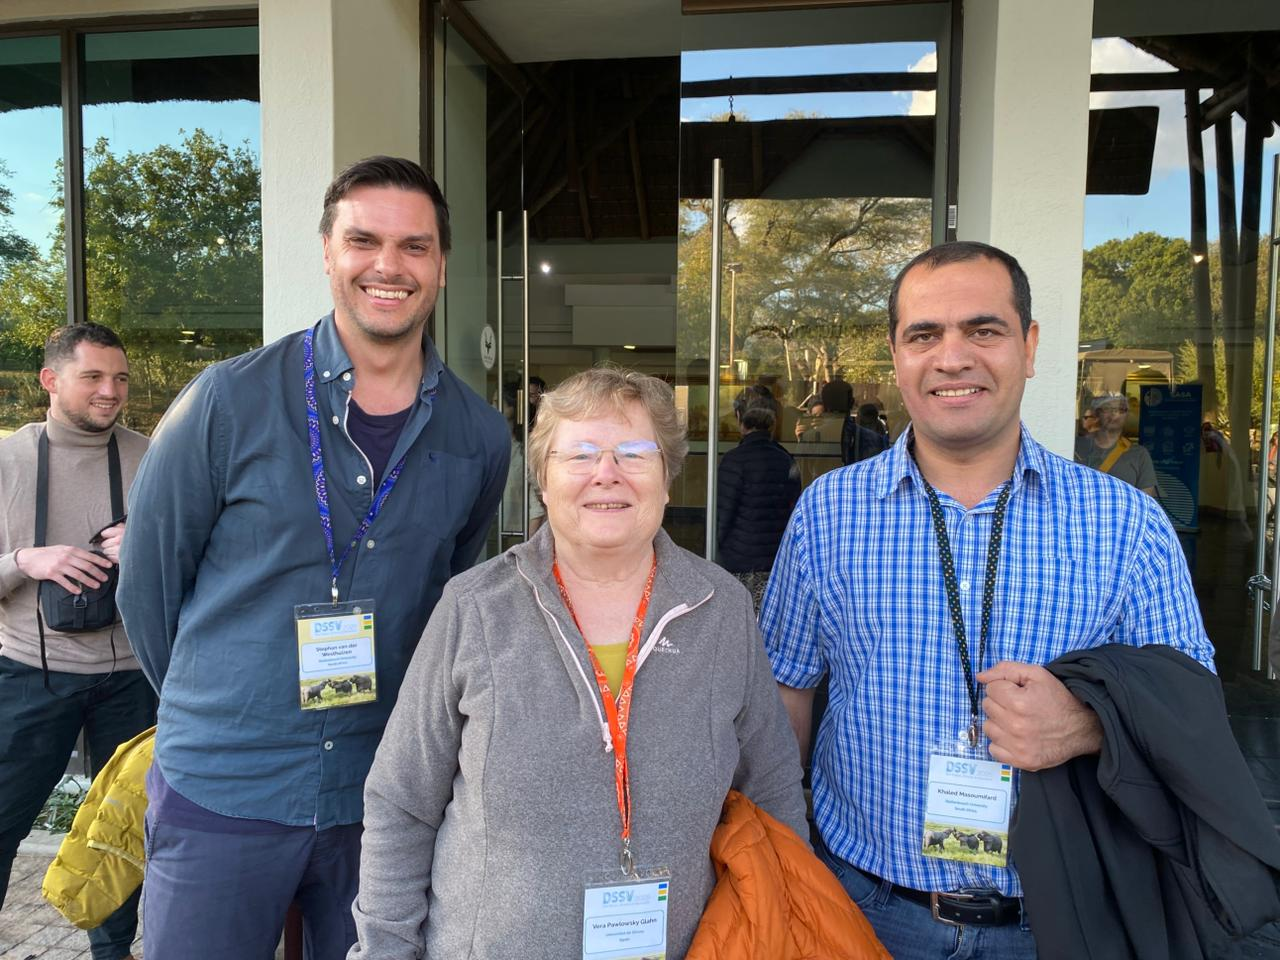
\includegraphics[width=0.4\linewidth]{slides/Vera.jpg}
}
\end{frame}


\begin{frame}{Debates}
\only<1>{
The CoDA school has redefined these principles several times in response to criticism.



        \begin{alertblock}{ (Zier \& Rehder (1998, 2001))}
     They pointed out that even Aitchison’s own earlier work did not strictly satisfy the later CoDA definition of scale invariance.
    \end{alertblock}


        \begin{alertblock}{ (Scealy \& Welsh 2014)}
      The CoDa Principles act as a \textbf{gatekeeping criterion}:
      valid and useful methods have been dismissed simply for not
      conforming to them.
 
      \vspace{0.2cm}
      This is \textbf{unusual, perhaps unique, in statistical
      data analysis}.
    \end{alertblock}
}
\end{frame}



\begin{frame}{One Idea: Transforming to Real Space}





\only<1>{
  \framesubtitle{A transformation $\mathcal{S}^{K-1} \to \mathbb{R}^{K-1}$ unlocks standard inference: regression, PCA, LDA}

  \vspace{0.2cm}
  \renewcommand{\arraystretch}{1.35}
  \setlength{\tabcolsep}{8pt}

  \begin{tabular}{>{\bfseries}l l >{\footnotesize\itshape\color{gray}}l}
    \toprule
    \rowcolor{mainblue}
    \color{white}Method &
    \color{white}Formula &
    \color{white}Reference \\
    \midrule

    \rowcolor{accentblue!20}
    ALR & $\log y_i - \log y_K$ & Aitchison (1982) \\

    \rowcolor{accentblue!20}
    CLR & $\log y_i - K^{-1}\sum_{j=1}^{K} \log y_j$ & Aitchison (1983) \\

    \rowcolor{accentblue!20}
    ILR & $\mathbf{H}\!\left(\log y_i - K^{-1}\sum_{j=1}^{K} \log y_j\right)$ & Egozcue et al.\ (2003) \\

    \midrule
  
    {\normalfont $\alpha$} &
    {\footnotesize $\mathbf{H}[K_\alpha^{-1}(\mathbf{y} \otimes \alpha)]$} &
    Tsagris et al.\ (2011) \\

    {\normalfont BC$_1$} &
    {\footnotesize $\lambda^{-1}\!\left[(y_i / y_K)^\lambda - 1\right]$} &
    Aitchison (2003) \\

    {\normalfont BC$_2$} &
    {\footnotesize $\theta^{-1}(y_i^\theta - 1)$} &
    Greenacre (2010) \\

    {\normalfont Hyper-spherical} &
    {\footnotesize $\arccos\!\left(\dfrac{y_i}{\prod_{j=i+1}^{K} y_j}\right)$} &
    Wang et al.\ (2007) \\

    {\normalfont Square root} &
    {\footnotesize $\sqrt{y_i}$} &
    Stephens (1982) \\

    \bottomrule
  \end{tabular}

  \vspace{0.2cm}
  {\small\textbf{Key:} ALR, CLR, ILR are the most widely used;
  all resolve singularity of $\Sigma_{\mathbf{X}}$ by mapping to unconstrained $\mathbb{R}^{K-1}$.}
}



\end{frame}








\begin{frame}{Machine learning for CoDA}
      \centering
      \vfill
      \textbf{\Large Machine learning for CoDA}
      \vfill
\end{frame}







\begin{frame}{Machine learning: Random Forest}

\begin{itemize}

\item \textbf{Why machine learning?}  
For responses that are compositional: many predictors with complex non-linear patterns that traditional models cannot capture.

\item \textbf{Common approaches}:  
Apply ML models without considering the simplex geometry, or transform data (with log-ratio transformations) to real space (risking distortion and bias).

\item \textbf{Why Random Forests?}  
RFs are flexible and their splitting rules can be easily adapted to respect the simplex structure.

\item PhD of van der Westhuizen (2024) inspired the idea to use tree splitting to account for coDA
\end{itemize}

    
\end{frame}



\begin{frame}{Random Forests framework}
 
\begin{itemize}
   \item[\textcolor{blue}{\large$\blacktriangleright$}]  Given a sample size $n$ and $m$ covariates:
    \[
        \mathbf{X} \in \mathbb{R}^{n \times m} \quad \text{(covariate matrix)}, \qquad
        \mathbf{Y} \in \mathbb{R}^{n \times k} \quad \text{(response matrix)}
    \]
    
  \item[\textcolor{blue}{\large$\blacktriangleright$}]  Each row of \( \mathbf{Y} \) is a compositional vector:
    \[
        Y_{i,j} > 0 \quad \text{for all } i, j, \qquad \sum_{j=1}^k Y_{i,j} = 1
    \]
        
  
     \item[\textcolor{blue}{\large$\blacktriangleright$}] Goal: learn a mapping
    \[
    \mathbf{x} \;\longrightarrow\; \mathbf{y}
    \]
    respecting the simplex geometry
    \vspace{0.8em}

    % \item[\textcolor{blue}{\large$\blacktriangleright$}] Approach: adapt \textbf{random forests} for compositional outputs
    % \vspace{0.8em}

     \item[\textcolor{blue}{\large$\blacktriangleright$}] After training:
    \begin{itemize}
        \item Predict compositional responses for new inputs
        \item Estimate conditional distribution of responses
    \end{itemize}

\end{itemize}
\end{frame}

\begin{frame}{Random Forest: Overview}

A \textbf{Random Forest} is an ensemble of decision trees, each trained on a
bootstrap sample of the data. Key tuning parameters include:

\vspace{0.5em}

\begin{itemize}
    \item \textbf{Number of trees} ($B$): more trees improve stability but increase cost
    \item \textbf{Tree depth} ($d_{\max}$): controls model complexity and overfitting
    \item \textbf{Minimum node size} ($n_{\min}$): minimum observations required to split a node
    \item \textbf{Covariates per split} ($m_{\text{try}}$): number of randomly selected covariates
    considered at each split; typically set to $\sqrt{p}$
\end{itemize}

\end{frame}

\begin{frame}{Random forest: tree}

\centering
\only<1>{

\begin{columns}
    \begin{column}{0.4\linewidth}
    
        \begin{figure}[h]
\centering
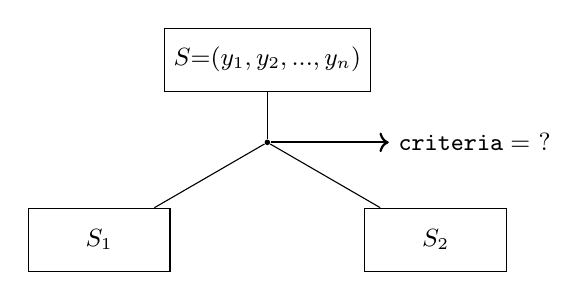
\begin{tikzpicture}[
    node distance=0.8cm,
    box/.style={rectangle, draw, minimum width=1.8cm, minimum height=0.8cm, text centered, font=\small},
    dot/.style={circle, fill=black, minimum size=2pt, inner sep=0pt},
    arrow/.style={->, thick}
]
% Main parent node
\node[box] (parent) {$S$=\\$(y_1, y_2, ..., y_n)$};
% Split point (dot in the middle)
\node[dot, below=0.6cm of parent] (split) {};
% Two child nodes
\node[box, below left=0.8cm and 1.2cm of split] (left) {$S_1$};
\node[box, below right=0.8cm and 1.2cm of split] (right) {$S_2$};
% Connections
\draw (parent) -- (split);
\draw (split) -- (left);
\draw (split) -- (right);
% Loss function arrow and equation
\node[right=1.5cm of split, font=\small] (loss) {$\texttt{criteria} = $ ?};
\draw[arrow] (split) -- (loss);
\end{tikzpicture}

\label{fig:decision_tree_split}
\end{figure}



    \end{column}
\begin{column}{0.6\linewidth}
\vspace{1cm}
$\qquad \qquad$A binary decision tree
\vspace

\resizebox{1\linewidth}{!}{%
        \begin{tikzpicture}[
  level/.style={sibling distance=60mm/#1},
  every node/.style={circle, draw, minimum size=8mm, font=\tiny},
  dots/.style={draw=none, font=\large}
]
\node {Root}
  child {
    node {L1}
    child {
      node {L2}
      child {
        node[dots] {$\vdots$}
      }
      child {
        node[dots] {$\vdots$}
      }
    }
    child {
      node {L2}
      child {
        node[dots] {$\vdots$}
      }
      child {
        node[dots] {$\vdots$}
      }
    }
  }
  child {
    node {R1}
    child {
      node {L2}
      child {
        node[dots] {$\vdots$}
      }
      child {
        node[dots] {$\vdots$}
      }
    }
    child {
      node {L2}
      child {
        node[dots] {$\vdots$}
      }
      child {
        node[dots] {$\vdots$}
      }
    }
  };
\end{tikzpicture}}
    \end{column}

    
\end{columns}


}

\end{frame}






\begin{frame}{}\only<1>{\frametitle{MSE splitting}

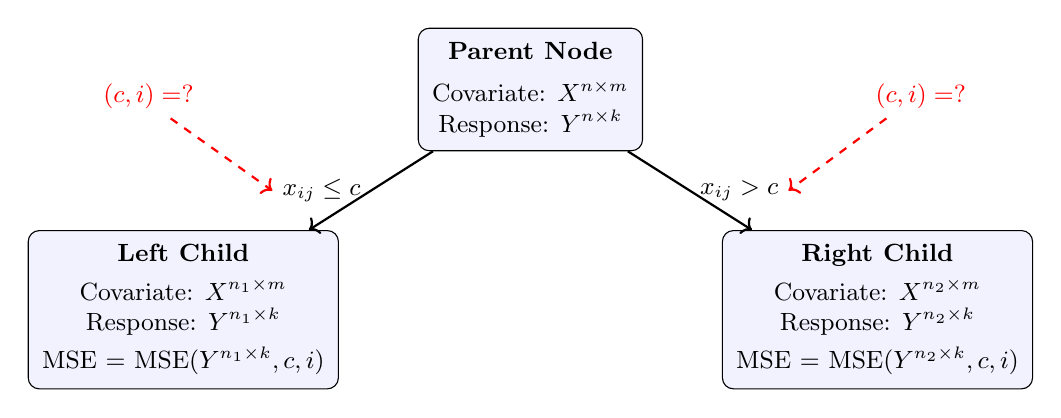
\begin{tikzpicture}[
  node distance=1cm and 1cm,
  every node/.style={font=\small},
  data/.style={rectangle, draw, align=center, fill=blue!5, rounded corners, inner sep=5pt},
  split/.style={->, thick},
  highlight/.style={->, red, thick, dashed}
  ]
  % Parent node
  \node[data] (parent) {
    \textbf{Parent Node} \\[0.15cm]
    Covariate: $X^{n \times m}$ \\ 
    Response: $Y^{n \times k}$
  };
  % Left child
  \node[data, below left=of parent] (left) {
    \textbf{Left Child} \\[0.1cm]
    Covariate: $X^{n_1 \times m}$ \\
    Response: $Y^{n_1 \times k}$ \\[0.1cm]
    MSE = $\text{MSE}(Y^{n_1 \times k},c,i)$
  };
  % Right child
  \node[data, below right=of parent] (right) {
    \textbf{Right Child} \\[0.1cm]
    Covariate: $X^{n_2 \times m}$ \\
    Response: $Y^{n_2 \times k}$ \\[0.1cm]
    MSE = $\text{MSE}(Y^{n_2 \times k},c,i)$
  };
  % Arrows
  \draw[split] (parent) -- node[midway, left] (leftlabel) {$x_{ij} \leq c$} (left);
  \draw[split] (parent) -- node[midway, right] (rightlabel) {$x_{ij} > c$} (right);
  
  % Optimize labels
  \node[red, left] (opt_i) at ([xshift=-1.5cm, yshift=1.2cm]leftlabel) {\textbf{ } $(c,i)=?$};
  \node[red, right] (opt_c) at ([xshift=1.5cm, yshift=1.2cm]rightlabel) {\textbf{} $(c,i)=?$};
  
  % Short highlight arrows from labels to split conditions
  \draw[highlight] (opt_i) -- (leftlabel.west);
  \draw[highlight] (opt_c) -- (rightlabel.east);
\end{tikzpicture}


}
\only<2>{

\frametitle{Split rule}
\begin{columns}[T]

  \column{0.8\textwidth}
 \begin{center}
\renewcommand{\arraystretch}{1.6}
\begin{tabular}{c|c>{\columncolor{purple!20}}cc>{\columncolor{purple!20}}cc|ccc|c}
\textbf{obs} & $x_1$ & \cellcolor{purple!50}$x_2$ & $x_3$ & \cellcolor{purple!20}$x_4$ & $x_5$ & $y_1$ & $y_2$ & $y_3$ & \textbf{child} \\
\hline
\rowcolor{blue!15}
1 & 0.8 & \textbf{1.2} & 3.4 & 0.5 & 2.1 & 0.60 & 0.25 & 0.15 & \textcolor{blue!80!black}{$\leftarrow$ left} \\
\rowcolor{blue!15}
2 & 2.3 & \textbf{2.7} & 1.1 & 4.2 & 0.9 & 0.10 & 0.70 & 0.20 & \textcolor{blue!80!black}{$\leftarrow$ left} \\
\rowcolor{blue!15}
3 & 1.5 & \textbf{3.1} & 2.9 & 1.8 & 3.3 & 0.45 & 0.45 & 0.10 & \textcolor{blue!80!black}{$\leftarrow$ left} \\
\rowcolor{red!15}
4 & 3.9 & \textbf{4.4} & 0.7 & 3.1 & 1.4 & 0.05 & 0.15 & 0.80 & \textcolor{red!80!black}{right $\rightarrow$} \\
\rowcolor{blue!15}
5 & 0.4 & \textbf{2.0} & 4.5 & 2.7 & 5.0 & 0.50 & 0.30 & 0.20 & \textcolor{blue!80!black}{$\leftarrow$ left} \\
\rowcolor{red!15}
6 & 2.1 & \textbf{5.6} & 3.8 & 0.3 & 2.2 & 0.02 & 0.08 & 0.90 & \textcolor{red!80!black}{right $\rightarrow$} \\
\rowcolor{red!15}
7 & 3.3 & \textbf{3.8} & 1.6 & 4.9 & 0.6 & 0.03 & 0.12 & 0.85 & \textcolor{red!80!black}{right $\rightarrow$} \\
\rowcolor{blue!15}
8 & 1.1 & \textbf{1.5} & 2.2 & 1.1 & 4.4 & 0.55 & 0.35 & 0.10 & \textcolor{blue!80!black}{$\leftarrow$ left} \\
\end{tabular}
\end{center}

  \column{0.22\textwidth}
  \vspace{1em}
  \begin{block}{Partition rule}
    Covariate 2: $i=2$ \\ Split value: $c =3.1$\\
    
  \end{block}
  \vspace{0.8em}
  \textcolor{blue!80!black}{\textbf{Left}} \\
  \hspace{0.5em} $x_2 \leq 3.1$ \\[0.2em]
  \hspace{0.5em} obs: 1, 2, 3, 5, 8 \\[0.6em]
  \textcolor{red!80!black}{\textbf{Right}} \\
   \hspace{0.5em} $x_2 > 3.1$ \\
  \hspace{0.5em} obs: 4, 6, 7


\end{columns}
}


\end{frame}




% %--- SLIDE 1: The data ---
% \begin{frame}{Growing a Tree: The Data}
% \begin{columns}[T]

%   \column{0.65\textwidth}
%   \begin{center}
%   \renewcommand{\arraystretch}{1.6}
%   \begin{tabular}{c|ccccc|ccc}
%   \textbf{obs} & $x_1$ & $x_2$ & $x_3$ & $x_4$ & $x_5$ & $y_1$ & $y_2$ & $y_3$ \\
%   \hline
%   1 & 0.8 & 1.2 & 3.4 & 0.5 & 2.1 & 0.60 & 0.25 & 0.15 \\
%   2 & 2.3 & 2.7 & 1.1 & 4.2 & 0.9 & 0.10 & 0.70 & 0.20 \\
%   3 & 1.5 & 3.1 & 2.9 & 1.8 & 3.3 & 0.45 & 0.45 & 0.10 \\
%   4 & 3.9 & 4.4 & 0.7 & 3.1 & 1.4 & 0.05 & 0.15 & 0.80 \\
%   5 & 0.4 & 2.0 & 4.5 & 2.7 & 5.0 & 0.50 & 0.30 & 0.20 \\
%   6 & 2.1 & 5.6 & 3.8 & 0.3 & 2.2 & 0.02 & 0.08 & 0.90 \\
%   7 & 3.3 & 3.8 & 1.6 & 4.9 & 0.6 & 0.03 & 0.12 & 0.85 \\
%   8 & 1.1 & 1.5 & 2.2 & 1.1 & 4.4 & 0.55 & 0.35 & 0.10 \\
%   \end{tabular}
%   \end{center}

%   \column{0.32\textwidth}
%   \vspace{1em}
%   \begin{block}{Setup}
%     Each node holds $n$ observations with $p$ covariates.
%   \end{block}
%   \vspace{0.8em}
%   \textbf{Response} $\mathbf{y}$ is compositional:
%   \[
%     \mathbf{y} = (y_1, y_2, y_3)
%   \]
%   \[
%     y_k \geq 0, \quad \textstyle\sum_k y_k = 1
%   \]
%   \vspace{0.4em}
%   Lives on the simplex $\mathcal{S}^2$.

% \end{columns}
% \end{frame}


% %--- SLIDE 2: Select covariates ---
% \begin{frame}{Step 1 — Select Covariates}
% \begin{columns}[T]

%   \column{0.65\textwidth}
%   \begin{center}
%   \renewcommand{\arraystretch}{1.6}
%   \begin{tabular}{c|c>{\columncolor{purple!20}}cc>{\columncolor{purple!20}}cc|ccc}
%   \textbf{obs} & $x_1$ & \cellcolor{purple!50}$x_2$ & $x_3$ & \cellcolor{purple!50}$x_4$ & $x_5$ & $y_1$ & $y_2$ & $y_3$ \\
%   \hline
%   1 & 0.8 & 1.2 & 3.4 & 0.5 & 2.1 & 0.60 & 0.25 & 0.15 \\
%   2 & 2.3 & 2.7 & 1.1 & 4.2 & 0.9 & 0.10 & 0.70 & 0.20 \\
%   3 & 1.5 & 3.1 & 2.9 & 1.8 & 3.3 & 0.45 & 0.45 & 0.10 \\
%   4 & 3.9 & 4.4 & 0.7 & 3.1 & 1.4 & 0.05 & 0.15 & 0.80 \\
%   5 & 0.4 & 2.0 & 4.5 & 2.7 & 5.0 & 0.50 & 0.30 & 0.20 \\
%   6 & 2.1 & 5.6 & 3.8 & 0.3 & 2.2 & 0.02 & 0.08 & 0.90 \\
%   7 & 3.3 & 3.8 & 1.6 & 4.9 & 0.6 & 0.03 & 0.12 & 0.85 \\
%   8 & 1.1 & 1.5 & 2.2 & 1.1 & 4.4 & 0.55 & 0.35 & 0.10 \\
%   \end{tabular}
%   \end{center}

%   \column{0.32\textwidth}
%   \vspace{1em}
%   \begin{block}{Random subspace}
%     At each node, draw $m \leq p$ covariates at random.
%   \end{block}
%   \vspace{0.8em}
%   \textcolor{purple!80!black}{\textbf{Selected:}} $x_2,\, x_4$
%   \vspace{0.6em}

%   \begin{itemize}[label={\ding{226}}]
%     \item Reduces correlation between trees
%     \item Only \textcolor{purple!80!black}{highlighted columns} are split candidates
%     \item Other columns are ignored at this node
%   \end{itemize}

% \end{columns}
% \end{frame}


% %--- SLIDE 3: Find the best split ---
% \begin{frame}{Step 2 — Find the Best Split}
% \begin{columns}[T]

%   \column{0.72\textwidth}
%   \begin{center}
%   \renewcommand{\arraystretch}{1.6}
%   \begin{tabular}{c|c>{\columncolor{purple!20}}cc>{\columncolor{purple!20}}cc|ccc|c}
%   \textbf{obs} & $x_1$ & \cellcolor{purple!50}$x_2$ & $x_3$ & \cellcolor{purple!20}$x_4$ & $x_5$ & $y_1$ & $y_2$ & $y_3$ & \\
%   \hline
%   \rowcolor{leftblue}
%   1 & 0.8 & \textbf{1.2} & 3.4 & 0.5 & 2.1 & 0.60 & 0.25 & 0.15 & \textcolor{blue!80!black}{$\leftarrow$ left} \\
%   \rowcolor{leftblue}
%   2 & 2.3 & \textbf{2.7} & 1.1 & 4.2 & 0.9 & 0.10 & 0.70 & 0.20 & \textcolor{blue!80!black}{$\leftarrow$ left} \\
%   \rowcolor{leftblue}
%   3 & 1.5 & \textbf{3.1} & 2.9 & 1.8 & 3.3 & 0.45 & 0.45 & 0.10 & \textcolor{blue!80!black}{$\leftarrow$ left} \\
%   \rowcolor{rightred}
%   4 & 3.9 & \textbf{4.4} & 0.7 & 3.1 & 1.4 & 0.05 & 0.15 & 0.80 & \textcolor{red!80!black}{right $\rightarrow$} \\
%   \rowcolor{leftblue}
%   5 & 0.4 & \textbf{2.0} & 4.5 & 2.7 & 5.0 & 0.50 & 0.30 & 0.20 & \textcolor{blue!80!black}{$\leftarrow$ left} \\
%   \rowcolor{rightred}
%   6 & 2.1 & \textbf{5.6} & 3.8 & 0.3 & 2.2 & 0.02 & 0.08 & 0.90 & \textcolor{red!80!black}{right $\rightarrow$} \\
%   \rowcolor{rightred}
%   7 & 3.3 & \textbf{3.8} & 1.6 & 4.9 & 0.6 & 0.03 & 0.12 & 0.85 & \textcolor{red!80!black}{right $\rightarrow$} \\
%   \rowcolor{leftblue}
%   8 & 1.1 & \textbf{1.5} & 2.2 & 1.1 & 4.4 & 0.55 & 0.35 & 0.10 & \textcolor{blue!80!black}{$\leftarrow$ left} \\
%   \end{tabular}
%   \end{center}

%   \column{0.25\textwidth}
%   \vspace{1em}
%   \begin{block}{Partition rule}
%     \textcolor{purple!80!black}{Best:} $x_2 \leq 3.5$
%   \end{block}
%   \vspace{0.8em}
%   \textcolor{blue!80!black}{\textbf{Left}} \hfill $x_2 \leq 3.5$\\[0.2em]
%   \hspace{0.5em} obs: 1,2,3,5,8 \\[0.6em]
%   \textcolor{red!80!black}{\textbf{Right}} \hfill $x_2 > 3.5$ \\[0.2em]
%   \hspace{0.5em} obs: 4,6,7
%   \vspace{0.6em}



% \end{columns}
% \end{frame}





\begin{frame}{}\only<1>{\frametitle{MSE splitting}

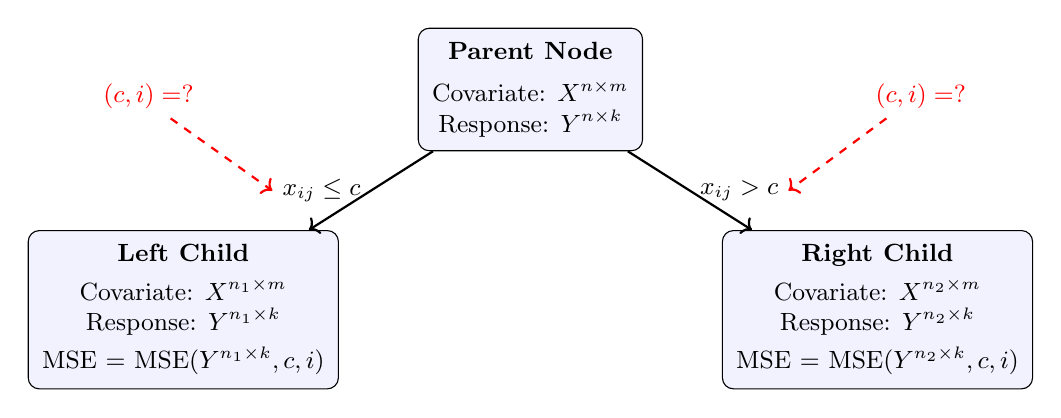
\begin{tikzpicture}[
  node distance=1cm and 1cm,
  every node/.style={font=\small},
  data/.style={rectangle, draw, align=center, fill=blue!5, rounded corners, inner sep=5pt},
  split/.style={->, thick},
  highlight/.style={->, red, thick, dashed}
  ]
  % Parent node
  \node[data] (parent) {
    \textbf{Parent Node} \\[0.15cm]
    Covariate: $X^{n \times m}$ \\ 
    Response: $Y^{n \times k}$
  };
  % Left child
  \node[data, below left=of parent] (left) {
    \textbf{Left Child} \\[0.1cm]
    Covariate: $X^{n_1 \times m}$ \\
    Response: $Y^{n_1 \times k}$ \\[0.1cm]
    MSE = $\text{MSE}(Y^{n_1 \times k},c,i)$
  };
  % Right child
  \node[data, below right=of parent] (right) {
    \textbf{Right Child} \\[0.1cm]
    Covariate: $X^{n_2 \times m}$ \\
    Response: $Y^{n_2 \times k}$ \\[0.1cm]
    MSE = $\text{MSE}(Y^{n_2 \times k},c,i)$
  };
  % Arrows
  \draw[split] (parent) -- node[midway, left] (leftlabel) {$x_{ij} \leq c$} (left);
  \draw[split] (parent) -- node[midway, right] (rightlabel) {$x_{ij} > c$} (right);
  
  % Optimize labels
  \node[red, left] (opt_i) at ([xshift=-1.5cm, yshift=1.2cm]leftlabel) {\textbf{ } $(c,i)=?$};
  \node[red, right] (opt_c) at ([xshift=1.5cm, yshift=1.2cm]rightlabel) {\textbf{} $(c,i)=?$};
  
  % Short highlight arrows from labels to split conditions
  \draw[highlight] (opt_i) -- (leftlabel.west);
  \draw[highlight] (opt_c) -- (rightlabel.east);
\end{tikzpicture}

\begin{align*}
    
(c^*, i^*) 
&=& \operatorname{argmin}_{i,c} \left( \text{MSE}(Y^{n_1 \times k},c,i) + \text{MSE}(Y^{n_2 \times k},c,i) \right)
\\
&=& \arg\min_{c,j} 
\left\{\frac{n_1(c,j)}{n}
\sum_{m=1}^k \sum_{i=1}^{n_1(c,j)} (y_{im}-\bar{y}_{m}^{n_1(c,j)})^2
+
\frac{n_2(c,j)}{n}
\sum_{m=1}^k \sum_{i=1}^{n_2(c,j)} (y_{im}-\bar{y}_{m}^{n_2(c,j)})^2
\right\}.
\end{align*}

}



\only<2>{ \frametitle{MSE splitting}

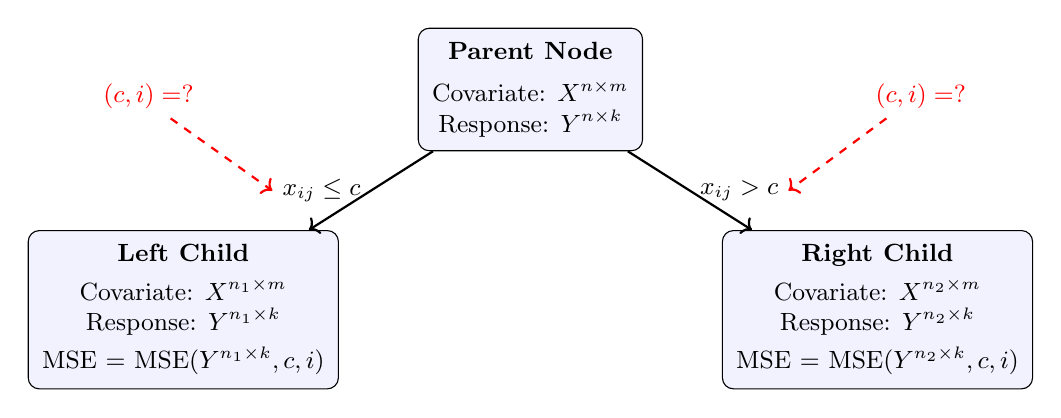
\begin{tikzpicture}[
  node distance=1cm and 1cm,
  every node/.style={font=\small},
  data/.style={rectangle, draw, align=center, fill=blue!5, rounded corners, inner sep=5pt},
  split/.style={->, thick},
  highlight/.style={->, red, thick, dashed}
  ]
  % Parent node
  \node[data] (parent) {
    \textbf{Parent Node} \\[0.15cm]
    Covariate: $X^{n \times m}$ \\ 
    Response: $Y^{n \times k}$
  };
  % Left child
  \node[data, below left=of parent] (left) {
    \textbf{Left Child} \\[0.1cm]
    Covariate: $X^{n_1 \times m}$ \\
    Response: $Y^{n_1 \times k}$ \\[0.1cm]
    MSE = $\text{MSE}(Y^{n_1 \times k},c,i)$
  };
  % Right child
  \node[data, below right=of parent] (right) {
    \textbf{Right Child} \\[0.1cm]
    Covariate: $X^{n_2 \times m}$ \\
    Response: $Y^{n_2 \times k}$ \\[0.1cm]
    MSE = $\text{MSE}(Y^{n_2 \times k},c,i)$
  };
  % Arrows
  \draw[split] (parent) -- node[midway, left] (leftlabel) {$x_{ij} \leq c$} (left);
  \draw[split] (parent) -- node[midway, right] (rightlabel) {$x_{ij} > c$} (right);
  
  % Optimize labels
  \node[red, left] (opt_i) at ([xshift=-1.5cm, yshift=1.2cm]leftlabel) {\textbf{ } $(c,i)=?$};
  \node[red, right] (opt_c) at ([xshift=1.5cm, yshift=1.2cm]rightlabel) {\textbf{} $(c,i)=?$};
  
  % Short highlight arrows from labels to split conditions
  \draw[highlight] (opt_i) -- (leftlabel.west);
  \draw[highlight] (opt_c) -- (rightlabel.east);
\end{tikzpicture}
\begin{itemize}
    \item 
MSE does not account for the simplex constraint.

\item 
\[V(X_i)=\frac{E(X_i)\left(1-E(X_i)\right)}{\alpha_0+1}\]
\end{itemize}

}

\end{frame}







\begin{frame}
\only<1>{
\frametitle{Dirichlet distribution}


\vspace{1em}

\begin{center}
\colorbox{green!10}{\parbox{0.95\textwidth}{
\begin{center}
\resizebox{\linewidth}{!}{%
\[
    f_{\mathbf{Z}}((z_1,\ldots,z_k); \boldsymbol{\alpha}) = \frac{\Gamma( \alpha_0)}{\prod_{i=1}^k \Gamma(\alpha_i)} \prod_{i=1}^k z_i^{\alpha_i - 1},
\quad  z_i \in [0, 1], \quad \sum_{i=1}^k z_i = 1,
\]
}
\end{center}
}}
\end{center}

\vspace{1.5em}

\begin{itemize}[itemsep=0.8em]


\item[\textcolor{blue}{\large$\blacktriangleright$}] The sum-constant requirement of the simplex is satisfied under the Dirichlet distribution.

\item[\textcolor{blue}{\large$\blacktriangleright$}] \textbf{Extensions available:} Zero-inflated Dirichlet and Kummer–Dirichlet
\end{itemize}
}

\end{frame}


\begin{frame}
\only<1>{\frametitle{Dirichlet log-likelihood splitting}

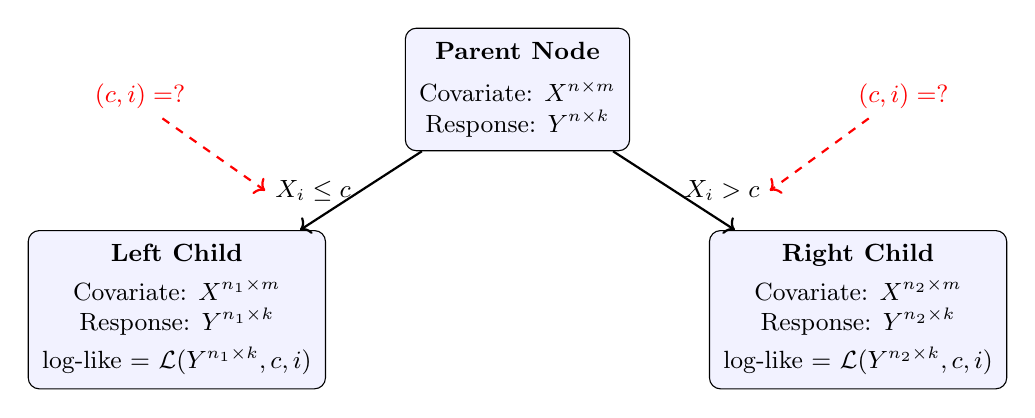
\begin{tikzpicture}[
  node distance=1cm and 1cm,
  every node/.style={font=\small},
  data/.style={rectangle, draw, align=center, fill=blue!5, rounded corners, inner sep=5pt},
  split/.style={->, thick},
  highlight/.style={->, red, thick, dashed}
  ]
  % Parent node
  \node[data] (parent) {
    \textbf{Parent Node} \\[0.15cm]
    Covariate: $X^{n \times m}$ \\ 
    Response: $Y^{n \times k}$
  };
  % Left child
  \node[data, below left=of parent] (left) {
    \textbf{Left Child} \\[0.1cm]
    Covariate: $X^{n_1 \times m}$ \\
    Response: $Y^{n_1 \times k}$ \\[0.1cm]
     log-like = $\mathcal{L}(Y^{n_1 \times k},c,i)$
  };
  % Right child
  \node[data, below right=of parent] (right) {
    \textbf{Right Child} \\[0.1cm]
    Covariate: $X^{n_2 \times m}$ \\
    Response: $Y^{n_2 \times k}$ \\[0.1cm]
     log-like = $\mathcal{L}(Y^{n_2 \times k},c,i)$
  };
  % Arrows
  \draw[split] (parent) -- node[midway, left] (leftlabel) {$X_{i} \leq c$} (left);
  \draw[split] (parent) -- node[midway, right] (rightlabel) {$X_{i} > c$} (right);
  
  % Optimize labels
  \node[red, left] (opt_i) at ([xshift=-1.5cm, yshift=1.2cm]leftlabel) {\textbf{ } $(c,i)=?$};
  \node[red, right] (opt_c) at ([xshift=1.5cm, yshift=1.2cm]rightlabel) {\textbf{} $(c,i)=?$};
  
  % Short highlight arrows from labels to split conditions
  \draw[highlight] (opt_i) -- (leftlabel.west);
  \draw[highlight] (opt_c) -- (rightlabel.east);
\end{tikzpicture}
\[
(c^*, i^*) = \operatorname{argmax}_{i,c} \left( \max_{\boldsymbol{\alpha}} \mathcal{L}(Y^{n_1 \times k},c,i) + \max_{\boldsymbol{\alpha}} \mathcal{L}(Y^{n_2 \times k},c,i) \right)
\]
}
\end{frame}

\begin{frame}{Prediction based on DirichletRF}

    
\begin{columns}[T]

% Left column - Graph
\begin{column}{0.45\textwidth}
\centering
\begin{tikzpicture}[
    node/.style={ellipse, draw, minimum width=1.2cm, minimum height=0.8cm, thick},
    leaf/.style={rectangle, draw, minimum width=1.8cm, minimum height=0.6cm, thick},
    arrow/.style={->, thick, blue},
    scale=0.75,
    every node/.style={transform shape}
]

% Root node
\node[node] (root) at (0,0) {};

% Level 1
\node[node] (n1) at (-2,-2) {};
\node (dots1) at (1,-2) {\vdots};

% Level 2
\node (dots2) at (-3,-3.5) {\vdots};
\node[node] (n2) at (-1,-4) {};

% Level 3
\node (dots3) at (-2.5,-5.5) {\vdots};
\node[node] (n3) at (0,-6) {};

% Level 4
\node (dots4) at (1,-7.5) {\vdots};
\node[leaf] (leaf) at (-1,-8) {$\{y_1, y_2, \ldots, y_{n_t^'}\}$};

% Arrows - traversal path highlighted
\draw[arrow, line width=1.5pt] (root) -- (n1);
\draw[arrow, dashed] (root) -- (dots1);
\draw[arrow, dashed] (n1) -- (dots2);
\draw[arrow, line width=1.5pt] (n1) -- (n2);
\draw[arrow, dashed] (n2) -- (dots3);
\draw[arrow, line width=1.5pt] (n2) -- (n3);
\draw[arrow, line width=1.5pt] (n3) -- (leaf);
\draw[arrow, dashed] (n3) -- (dots4);

\end{tikzpicture}
\end{column}

% Right column - Explanation
\begin{column}{0.52\textwidth}
\small

\textbf{Process:}
\begin{itemize}
\item[1)] Start at root node
    \item[2)] Traverse tree based on decision rules
    \item[3)] Reach terminal node with observations
\end{itemize}

\vspace{0.4cm}

\textbf{Default Approach:}
\begin{itemize}
    \item Mean: $\hat{y} = \frac{1}{n_t^'}\sum_{i=1}^{n_t^{'}} y_i$
    \item Expectation: $\text{E}(Y_i) = \frac{\hat{\alpha}_i}{\sum_{j+1}^k\hat{\alpha}_i}$
    \item Random Forest: average across trees
\end{itemize}

\vspace{0.4cm}

\textbf{Distributional Approach:}
\begin{itemize}
    \item Collect terminal nodes from all trees
    \item Construct empirical probability function
\end{itemize}

\end{column}

\end{columns}

\end{frame}










%-----------------------------------------------------------------------------
%===================================================
% Comparison Results


\begin{frame}{Comparison Results}
      \centering
      \vfill
      \textbf{\Large Comparison Results}
      \vfill
\end{frame}

\begin{frame}{Performance Evaluation and Transformations}

To evaluate DirichletRF's performance, we compare it with two alternative approaches:
\begin{itemize}
    \item[1)] \textbf{ILR-RF:} A Random Forest model based on log-ratio transformations. 
    The compositional data are first transformed into the ILR
    space. Then, a standard Random Forest is applied to the transformed data, and 
    finally, the predictions are mapped back to the simplex for interpretation.

    \item[2)] \textbf{Dirichlet Regression:} A parametric approach that, 
    works directly on the simplex without requiring any transformation.
\end{itemize}

\end{frame}




\begin{frame}{Evaluation Metrics}

To compare these models, we used  the Aitchison Distance.
\vspace{0.2cm}
\[
AC = \frac{1}{n} \sum_{i=1}^n \sqrt{\sum_{j=1}^k \left(\log\frac{Y_{ij}}{g(\mathbf{Y}_i)} - \log\frac{\hat{Y}_{ij}}{g(\hat{\mathbf{Y}}_i)}\right)^2},
\]
\[
\text{where} \quad g(\mathbf{Y}_i) = \left(\prod_{j=1}^k Y_{ij}\right)^{1/k}
\]


\vspace{0.3cm}
\textbf{Interpretation:} Lower values for this metric indicate better predictive accuracy.
\end{frame}








\begin{frame}{}

    \only<1>{
  
    \textbf{Simple structure simulations}: We use a simple dataset with $3$ Covariate variables, $X_1,X_1, X_{3}$ and with a $3$-dimensional response, $(Y_1,\,Y_2,\,Y_3)$ such that $Y_1+Y_2+Y_3 = 1$. The response is assumed to follow a Dirichlet distribution with the following parameters:
\[
\alpha_1 = 1 + 2 X_1,\quad \alpha_2 =1 + 0.5 X_2,\quad \alpha_3 = 1 + X_3.
\]
\[
(Y_1,\,Y_2,\,Y_3)\sim Dirichlet(\alpha_1,\alpha_2,\alpha_3)
\]
    }
    \only<2>{
      
Dirichlet Regression performed better than the other models. This result makes sense, because the data was generated using a Dirichlet distribution with a linear structure.


But, Dirichlet Random Forest does not perform well in this case — in fact, it gives the worst performance in terms of Aitchison Distance and RMSE.
\begin{table}[htbp]
\centering
\small 
\begin{tabular}{|l|l|c|c|}
\hline
$N$ & Model & Aitchison Distance & Train-Test \\
\hline
\multirow{3}{*}{200} 
    & ILR-RF & 1.303 (0.143) & 0.686 \\
    & \textcolor{blue}{Dirichlet Regression} & \textcolor{blue}{\textbf{1.233} (0.139)} & \textcolor{blue}{\textbf{0.030}} \\
    & \texttt{Dirichlet-RF} & 1.451 (0.153) & 0.600 \\
\hline
\multirow{3}{*}{500}
    & ILR-RF & 1.284 (0.077) & 0.685 \\
    & \textcolor{blue}{Dirichlet Regression} & \textcolor{blue}{\textbf{1.234} (0.078)} & \textcolor{blue}{\textbf{0.035}} \\
    & \texttt{Dirichlet-RF} & 1.450 (0.077) & 0.616 \\
\hline
\multirow{3}{*}{2000}
    & ILR-RF & 1.252 (0.032) & 0.654 \\
    & \textcolor{blue}{Dirichlet Regression} & \textcolor{blue}{\textbf{1.209} (0.032)} & \textcolor{blue}{\textbf{0.006}} \\
    & \texttt{Dirichlet-RF} & 1.431 (0.041) & 0.596 \\
\hline
\end{tabular}
\caption{Values represent the means and (standard deviations) of the metrics for test datasets. Train-Test Diff represents the absolute difference between train and test Aitchison Distance, indicating model generalisation capability.}
\label{tab:performance-comparison1}
\end{table}}

    \only<3>{
    	    

    
    Complex structure synthetic simulations: The dataset consisted of 10 predictor variables \((X_1, \ldots, X_{10})\), with only the first three variables \((X_1, X_2, X_3)\) being truly informative for predicting the compositional response. The three-component compositional response vector $\mathbf{Y} = (Y_1,Y_2,Y_3)$ was constructed through complex non-linear transformations of the informative Covariates. }
    \end{frame}
\begin{frame}
    \only<1>{

\begin{columns}
\begin{column}{0.5\linewidth}

% where \( \mathcal{N}(\mu_i, 0.5^2) \) represents a normally distributed random variable with mean \( \mu_i \) and standard deviation \( 0.5 \), and \( \epsilon \) is a small positive constant ensuring non-negativity.  
% The compositional response variables \( Y_1, Y_2, Y_3 \) are then obtained via the normalisation:
We generate the variables \( Z_1, Z_2, Z_3 \) as follows:  
\[
Z_i = \max(\epsilon, \mathcal{N}(\mu_i, 0.5)), \quad 
\]
\[
Y_i = \frac{Z_i}{Z_1 + Z_2 + Z_3}, \quad  i = 1,2,3.
\]
% This transformation ensures that \( (Y_1, Y_2, Y_3) \) lies within the unit simplex, preserving the compositional structure of the data.
\end{column}
		\begin{column}{0.5\linewidth}

\begin{align*}
\mu_{1j} &= g(2(1 + \sin(x_{1j}))+x_{2j}^3) \\
\mu_{2j} &= g(1 + 2.5\exp(x_{3j})+x_{1j}^2) \\
\mu_{3j} &= g(1 + (1+x_{2j})^2+x_{3j}^4)
\end{align*}

\end{column}

\end{columns}

Where
\[
g(x_{ij}) =
\begin{cases} 
    2, & x_{ij} < \text{Quantile}(x_i, 0.3) \\
    3, & \text{Quantile}(x_i, 0.3) \leq x_{ij} <\text{Quantile}(x_i, 0.6) \\
    4, & \text{Quantile}(x, 0.6) \leq x_{ij} \leq \text{Quantile}(x_i, 0.8) \\
    1, & x_i > \text{Quantile}(x_i, 0.8)
\end{cases}
\]

}
\end{frame}
\begin{frame}
\only<1>{

In this complex scenario, the results are reversed. Our Dirichlet-RF is now the best model, and Dirichlet Regression is the worst.
\begin{table}[htbp]
\centering
\small 
\begin{tabular}{|l|l|c|c|}
\hline
$N$ & Model & Aitchison Distance & Train-Test \\
\hline
\multirow{3}{*}{200} 
    & ILR-RF & 0.670 (0.151) & 0.364 \\
    & Dirichlet Regression & 0.826 (0.155) & 0.068 \\
    & \textcolor{blue}{\texttt{Dirichlet-RF}} & \textcolor{blue}{\textbf{0.659} (0.152)} & \textcolor{blue}{0.221} \\
\hline
\multirow{3}{*}{500}
    & ILR-RF & 0.618 (0.072) & 0.334 \\
    & Dirichlet Regression & 0.790 (0.075) & 0.029 \\
    & \textcolor{blue}{\texttt{Dirichlet-RF}} & \textcolor{blue}{\textbf{0.606} (0.068)} & \textcolor{blue}{0.201} \\
\hline
\multirow{3}{*}{2000}
    & ILR-RF & 0.557 (0.044) & 0.301 \\
    & Dirichlet Regression & 0.785 (0.044) & 0.016 \\
    & \textcolor{blue}{\texttt{Dirichlet-RF}} & \textcolor{blue}{\textbf{0.544} (0.044)} & \textcolor{blue}{0.178} \\
\hline
\end{tabular}
\caption{Train-Test Diff represents the absolute difference between train and test Aitchison Distance.}
\label{tab:performance-comparison}
\end{table}
}
\end{frame}



\begin{frame}{Learning Curve}
\only<1>{


\begin{figure}
    \centering
    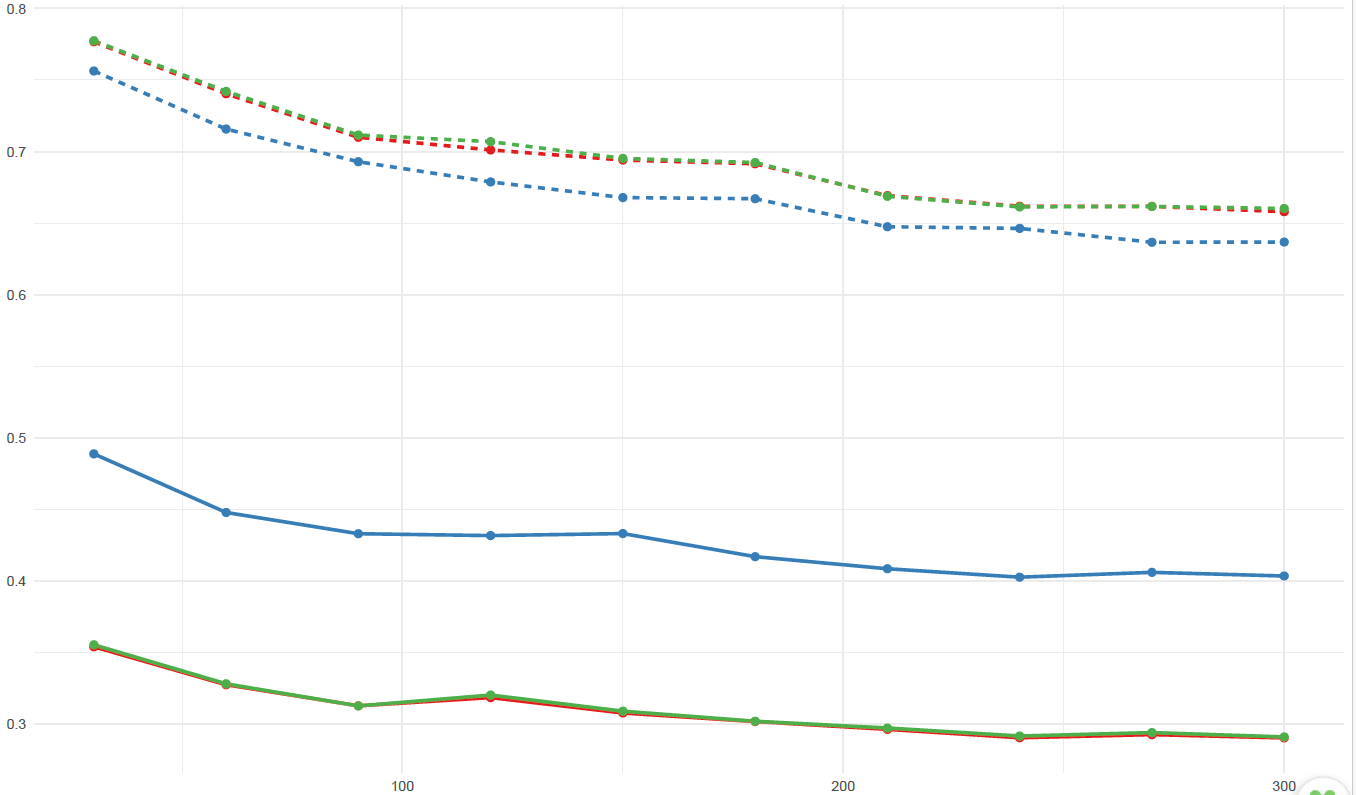
\includegraphics[width=0.75\linewidth]{Learning_curve.png}
    \caption{Aitchison distance as a function of training sample size for all three 
    Random Forest models.}
    \label{fig:enter-label}
\end{figure}
}
\end{frame}




% \begin{frame}
% \only<1>{
% \note{I am not sure to include this slide:

% And for further evaluation of \texttt{Dirichlet-RF}, we also looked at its performance in terms of covariate selection.

% Here, you can see how often each covariate was selected for splitting across all trees, and how much, on average, it contributed to increasing the log-likelihood.

% As I mentioned earlier, only three of the variables were informative — and \texttt{Dirichlet-RF} was able to clearly identify them with high importance.}
% \begin{table}[htbp]
% \centering
% \begin{tabular}{|c|c|c|}
% \hline
% \textbf{Covariate} & \small{Log-Likelihood Importance} & \small{Frequency-Based Importance} \\
% \hline
% \textcolor{blue}{$X_1$} & \textcolor{blue}{225.039} & \textcolor{blue}{14} \\
% \textcolor{blue}{$X_2$} & \textcolor{blue}{303.618} & \textcolor{blue}{21} \\
% \textcolor{blue}{$X_3$} & \textcolor{blue}{272.036} & \textcolor{blue}{19} \\
% \textcolor{red}{$X_4$} & \textcolor{red}{16.839}  & \textcolor{red}{2}  \\
% \textcolor{red}{$X_5$} & \textcolor{red}{9.972}   & \textcolor{red}{2}  \\
% \textcolor{red}{$X_6$} & \textcolor{red}{15.649}  & \textcolor{red}{3}  \\
% \textcolor{red}{$X_7$} & \textcolor{red}{0}   & \textcolor{red}{0}  \\
% \textcolor{red}{$X_8$} & \textcolor{red}{40.240}  & \textcolor{red}{6}  \\
% \textcolor{red}{$X_9$} & \textcolor{red}{5.369}   & \textcolor{red}{1}  \\
% \textcolor{red}{$X_{10}$} & \textcolor{red}{23.295}  & \textcolor{red}{3}  \\
% \hline
% \end{tabular}
% \caption{Variable importance scores based on log-likelihood improvement and selection frequency, averaged across all trees in the \texttt{Dirichlet-RF}.}

% \label{tab:variable-importance}
% \end{table}

% }
% \end{frame}






\begin{frame}{Implementation \& Code Access}
\note{This model was developed in Julia, and the full code is available on GitHub at the link provided.

We chose Julia mainly because of its strong computational performance. Implementing the model directly in R or Python would be much slower.

However, if you're working in R or Python, you can still use the model by calling the Julia functions from those languages.
We've included clear instructions in the repository, especially on how to connect Julia with R.

We're also planning to develop an R package with a C++ backend, which we hope to submit to CRAN, so the model will be even easier for R users to access.}
\vspace{1em}

\begin{itemize}[itemsep=1em]
\item[\textcolor{blue}{\large$\blacktriangleright$}] Model developed in \textbf{Julia} for computational efficiency

\item[\textcolor{blue}{\large$\blacktriangleright$}] Code available on \href{https://github.com/Xaleed/DirichletRandomForestJulia.git}{\textcolor{blue}{\textbf{GitHub}}}:

\textcolor{blue}{\small{https://github.com/Xaleed/DirichletRandomForestJulia.git}}
  \begin{center}

    \qrcode{https://github.com/Xaleed/DirichletRandomForestJulia.git}
 \end{center}



\end{itemize}

\vspace{1.5em}

\end{frame}


\begin{frame}{Alternative to MLE}
    \only<1>{
    \begin{block}{}
        One simple way to address this issue is to use the method of moments (MoM) as an alternative to maximum likelihood estimation (MLE). MoM gives an approximate solution but is much faster to compute.
    \end{block}
     \begin{block}{}
        We can also combine both approaches — instead of using MoM in all nodes, we can selectively apply it only in nodes where we expect its results to be close to MLE. This helps reduce computation while still keeping good accuracy.
    \end{block}
            \resizebox{0.65\linewidth}{!}{%

\begin{table}[htbp]
\centering

\begin{tabular}{|l|c|c|c|c|}
\hline
\multirow{2}{*}{Metric} & \multicolumn{2}{c|}{MLE} & \multicolumn{2}{c|}{MoM} \\
\cline{2-5}
 & (Train) & (Test) & (Train) & (Test) \\
\hline
Aitchison Distance & 0.3901 & 0.7391 & 0.4068 & 0.7457 \\
\hline
\end{tabular}
\end{table}}



}
\end{frame}



% \begin{frame}[plain]
% % \begin{center}
% %    
\includegraphics[width=5cm]{logo.png} % Optional logo
% %    \end{center}
%   \begin{center}
%       \vspace{2cm}

%     {\Huge \textbf{Thank You!} \par}
%     % \vspace{1cm}
%     % {\Large Questions or Comments? \par}
%     \vspace{1cm}
   
    
%     \qrcode{https://github.com/Xaleed/DirichletRandomForestJulia.git}
%    % \texttt{khaledmasoumifard@sun.ac.za}
%   \end{center}
% \end{frame}






% %
{
  \setbeamercolor{page number in head/foot}{fg=background canvas.bg}
  \begin{frame}
    \begin{tikzpicture}[remember picture, overlay]
      \node[anchor=north west, xshift=1em, yshift=-1em] at (current page.north west) {
        
\includegraphics[width=3cm]{logo.png}
      };
    \end{tikzpicture}

    \titlepage


      \begin{center}
    %    
\includegraphics[width=0.15\linewidth]{slides/DirichletRF.jpg}
    \qrcode[height=2.8cm]{https://github.com/Xaleed/DirichletRF.git}

    \vspace{0.1cm}

    {\small GitHub repository}

  \end{center}
  \end{frame}
}


\begin{frame}{What is This Talk About?}
% \note{
% Good morning, and thank you for joining this talk. It is about developing DDRF, which is part of my postdoc project at Stellenbosch University, in collaboration with Stephan and Professor Lubbe.


% In a nutshell, I’ll shortly refer what composistional data is? I will explain why is it reasonable to develop a random forest model for composiational data?
% I will some comparison result?}

\vspace{2em}

\nocite{In a nutshell, I will first talk about what compositional data are. Then, I will give a short literature review, including a brief history of compositional data and how this field developed. After that, I will move to the machine learning part, with a particular focus on Random Forests, and explain the model that we developed. I will also present some comparative results, where I compare our model with existing approaches. Finally, I will briefly introduce the R package that we developed.}

\vspace{1.5em}
\begin{itemize}
 
  \item[\textcolor{blue}{\large$\blacktriangleright$}] \textbf{Compositional data} -- Key characteristics and modeling challenges
    \vspace{1em}

    
  \item[\textcolor{blue}{\large$\blacktriangleright$}] \textbf{Machine learning: Random Forest} Modeling complex relationships
    \vspace{1em}
     \item[\textcolor{blue}{\large$\blacktriangleright$}] \textbf{ Dirichlet Random Forest model} -- Introduction and motivation
  \vspace{1em}

  \item[\textcolor{blue}{\large$\blacktriangleright$}] \textbf{Comparison results} -- Evaluating model performance
    \vspace{1em}
  \item[\textcolor{blue}{\large$\blacktriangleright$}] \textbf{
  DirichletRF R package}
\end{itemize}


\vspace{2em}

\end{frame}

% %

\begin{frame}{Compositional data}
\only<1>{
\note{
IFirst of all we should know what simplex space is, I will frequently refer to simplex space. 
A simplex space is  collection of vectors with non-negative values that always sum to a constant.
This space is known as the \emph{simplex} and it is common to set \( k = 1 \).
We refer to data from this space as \emph{compositional data}.

The problem I'm going to talk about is how can we apply a random forest to this space and why is this important?
}


\vspace{1em}

A simplex is a convex space of all vectors with non-negative components that sum to a constant. 



\begin{center}
\colorbox{blue!10}{\parbox{0.8\textwidth}{
\begin{center}
\[
S^c_k = \left\{ (y_1, \dots, y_k)^\top \in \mathbb{R}^k \,\middle|\, y_i \geq 0, \ \sum_{i=1}^k y_i = \textcolor{blue}{c} \right\}
\]
\end{center}
}}
\end{center}



 It is common to set \(  \textcolor{blue}{c = 1} \). We refer to data from this space as \emph{compositional data}.
 

}



\only<2>{

\textbf{A practical view of compositional data}

\vspace{0.3cm}

Let $\mathbf{Y} = (Y_1, Y_2, \dots, Y_K)$ be a vector with positive components.

\vspace{0.3cm}

The compositional transformation is defined as:
\[
\mathbf{S} =
\left(
\frac{Y_1}{\sum_{i=1}^K Y_i}, \dots,
\frac{Y_K}{\sum_{i=1}^K Y_i}
\right)
\]

\vspace{0.3cm}

This vector lies in the simplex space.

\vspace{0.5cm}

However, in this transformation we lose information about the \textbf{absolute scale}, and we cannot uniquely recover the original vector.

But we preserve the \textbf{relative information}.
In particular, for any two components $i$ and $j$:
\[
\frac{Y_i}{Y_j} = \frac{S_i}{S_j}
\]


\note{
Improved spoken version

We can also define compositional data in a more practical way.

Suppose we have a vector with non-negative components and no other restrictions.

If we divide each component by the total sum, we obtain a new vector that belongs to the simplex space.

This new vector is a compositional representation of the original data.

An important point is that we cannot recover the original vector uniquely from its compositional form.

In this transformation, we lose information about the absolute scale of the data.

However, what we can fully preserve is the relative information.

In particular, the ratios between components remain exactly the same after normalization.

So for any two components, the ratio is identical in both representations.

It is commonly assumed in this field that absolute values are not important.

The only meaningful information in compositional data is the relative information between components.
}


}

% \only<3>{
% \vspace{.2cm}
%    \textbf{Example}: consider 
% \(
% \mathbf{Y} = (2000, 3000, 5000),
% \)
% which represents the amount of money (in dollars) allocated to \textit{stocks}, \textit{bonds}, and \textit{cash} in an investment portfolio.  

% Then the following vector is a compositional data:
% \begin{align*}
% \scalebox{1.2}{$\left(\frac{2000}{2000+3000+5000},\;\frac{3000}{2000+3000+5000},\;\frac{5000}{2000+3000+5000}\right)$} = (0.2, 0.3, 0.5)
% \end{align*}

% \medskip

% Multiply by 100:
% \[
% 100 \cdot \mathbf{s}(\mathbf{Y}) = (20, 30, 50)
% \]

% \medskip

% Same proportions, different scale (percentages).
% \note{
% Here we see a portfolio allocation example.

% After normalization, we obtain proportions of total investment.

% Multiplying by 100 expresses them as percentages, which are more intuitive in finance.

% The relative allocation (20\%, 30\%, 50\%) remains unchanged regardless of the total invested amount.
% }
% }


\only<3>{
\note{Confirm:In this slide, consider a job application pool of 50 applicants. Among them, 10 have a mathematics background, 15 have a statistics background, and 25 have a computer science background.

If we normalize this vector by dividing each component by the total sum, we obtain a compositional vector.

Each component corresponds to the proportion of applicants with a different academic background.

By multiplying this vector by 100, we obtain percentages. For example, 20% of the applicants have a mathematics background.

The important point is that the information remains the same, but the scale changes—from proportions to percentages.

In general, multiplying a compositional vector by any positive constant does not change the relative information; it only changes the scale.

Now, this simple normalization step looks simple, but it has a very important statistical consequence.
}

Consider a job application pool of $50$ applicants classified by academic background.
\vspace{0.3cm}

\begin{columns}
    \begin{column}{0.4\textwidth}
        \[
        \mathbf{Y} = (10, 15, 25)
        \]
    \end{column}
    \begin{column}{0.5\textwidth}
        \begin{tabular}{lr}
            Mathematics & 10 \\
            Statistics  & 15 \\
            Computer Science & 25 \\
        \end{tabular}
    \end{column}
\end{columns}

\vspace{0.3cm}
We normalize this vector to obtain a compositional representation:
\vspace{0.2cm}

\begin{columns}
    \begin{column}{0.5\textwidth}
        \[
        \mathbf{s}(\mathbf{Y}) = \left(\frac{10}{50}, \frac{15}{50}, \frac{25}{50}\right)
        \]
    \end{column}
    \begin{column}{0.4\textwidth}
        \[
        = (0.2, 0.3, 0.5)
        \]
        Interpreted as proportions.
    \end{column}
\end{columns}

\vspace{0.2cm}
Multiplying by $100$ gives percentages:
\vspace{0.2cm}

\begin{columns}
    \begin{column}{0.5\textwidth}
        \[
        100 \cdot \mathbf{s}(\mathbf{Y}) = (20, 30, 50)
        \]
    \end{column}
    \begin{column}{0.4\textwidth}
        \textbf{Key idea:} The information is identical — only the scale changes.
    \end{column}
\end{columns}


}

\end{frame}


% \begin{frame}{Statistical problems with compositional data}
% 1)spurouis corelation
% 2)The (sample) covariance matrix of the data is singular with rank equal to $D - 1$, since
% \[
% \sum_{i=1}^{D} \operatorname{cov}(y_1, y_i)
% = \operatorname{cov}\left(y_1, \sum_{i=1}^{D} y_i \right)
% = \operatorname{cov}(y_1, 1)
% = 0,
% \]
% or equivalently,
% \[
% \sum_{i=2}^{D} \operatorname{cov}(y_1, y_i)
% = -\operatorname{var}(y_1),
% \]
% where each $y_i$ is a component of the composition $\mathbf{y}$.
% 3) Evidently, the problems and issues associated
% with compositional data are too numerous to list here and this is beyond the scope of
% this review paper.

    
% \end{frame}

% \begin{frame}{What methodology is more approperiate?}
% Aitchison suugest to tranfer data...

% dicson had another idea...

% a long argue staeted between them ... and finally Aitchison used stupid word and dicson lift the discussion for evere...
% Aitchison keep continue work on his idea and bring a lot of attention this his idea so many researcher for a while tried to his idea ... 
% aclsy and .. belive this made bad effect on the the field ... and for a while many researcher tried to say you have to use transformation methods...

% They belived 
% \end{frame}










% %% =============================================================
%  SPURIOUS CORRELATION
%  % =============================================================
%  SPURIOUS CORRELATION
%  % =============================================================
%  SPURIOUS CORRELATION
%  \input{slides/Spurious_correlation}
% =============================================================


% ------------------------------------------------------------------
%  SLIDE 1 – Spurious Correlation (Pearson)
% ------------------------------------------------------------------

\begin{frame}{Correlation}
  \note{
Now, I extend this example to 500 different job opportunities.

In other words, I generated 500 similar datasets, although only a few rows are shown in this table. Each row represents the number of applicants for one job opportunity.

If we calculate the correlation between applicants with a Mathematics background and applicants with a Statistics background in the original count data, the result is close to zero, as you can see.

This is exactly what we expect, because the variables were generated independently.

Now, if we transform the same data into the simplex space, we obtain a very different result. The Mathematics and Statistics components become strongly negatively correlated.

So, what does this correlation actually mean? What kind of information can we extract from it?

This is not an easy question to answer.

A common mistake is to interpret this as an ordinary correlation between applicants from Mathematics and Statistics backgrounds, as we would do in a standard data table.

However, this interpretation is misleading.

These types of correlations are known as spurious correlations.

      }
\only<1>{
  \begin{columns}
    \column{0.5\textwidth}
    \textbf{Original Data (Counts)}

    \vspace{0.2cm}
    \begin{center}
    \begin{tabular}{ccc}
      \hline
      Math & Stats & CS \\
      \hline
      48  & 230 & 59  \\
      286 & 181 & 73  \\
      286 & 98  & 147 \\
      35  & 14  & 12  \\
      255 & 104 & 235 \\
      $\vdots$ & $\vdots$ & $\vdots$ \\
      \hline
    \end{tabular}
    \end{center}

    \vspace{0.2cm}
    \[
      \mathrm{corr}(\text{Math},\,\text{Stats}) = 0.087
    \]

    \column{0.5\textwidth}
    
  \end{columns}


}
\only<2>{
\begin{columns}
    \column{0.5\textwidth}
    \textbf{Original Data (Counts)}

    \vspace{0.2cm}
    \begin{center}
    \begin{tabular}{ccc}
      \hline
      Math & Stats & CS \\
      \hline
      48  & 230 & 59  \\
      286 & 181 & 73  \\
      286 & 98  & 147 \\
      35  & 14  & 12  \\
      255 & 104 & 235 \\
      $\vdots$ & $\vdots$ & $\vdots$ \\
      \hline
    \end{tabular}
    \end{center}

    \vspace{0.2cm}
    \[
      \mathrm{corr}(\text{Math},\,\text{Stats}) = 0.087
    \]

    \column{0.5\textwidth}
    \textbf{Compositional Data (Normalized to 100)}

    \vspace{0.2cm}
    \begin{center}
    \begin{tabular}{ccc}
      \hline
      Math & Stats & CS \\
      \hline
      14.2 & 68.2 & 17.5 \\
      53.0 & 33.5 & 13.5 \\
      53.9 & 18.5 & 27.7 \\
      57.4 & 23.0 & 19.7 \\
      42.9 & 17.5 & 39.6 \\
      $\vdots$ & $\vdots$ & $\vdots$ \\
      \hline
    \end{tabular}
    \end{center}

    \vspace{0.2cm}
    \[
      \mathrm{corr}(X_{\text{math}},\, X_{\text{stats}}) = -0.874
    \]
  \end{columns}

}

\end{frame}

\end{frame}
\begin{frame}{Spurious Correlation}

 


\only<1>{
\note{Remove this slide:
Spurious correlation

One important consequence of working with compositional data is spurious correlation.

This phenomenon was introduced by Pearson in 1897.

He showed that ratios that share a common denominator can appear correlated, even when the original variables are completely independent.

To see this, let us consider three independent random variables: A, B, and C.

Now suppose we construct two new variables by dividing A by C and B by C.

Even though A and B are independent, these two ratios can become correlated because they share the same denominator.

}
  \begin{block}{Pearson (1897)}
    Ratios that share a common denominator are correlated even when the
    original variables are \emph{completely independent}.
  \end{block}

  \vspace{0.4em}
  \textbf{Simple illustration:} Let $A$, $B$, $C$ be mutually independent. Then:
  \[
    \operatorname{corr}\!\left(\frac{A}{C},\;\frac{B}{C}\right) \neq 0
  \]
  \vspace{0.2em}
  The shared denominator $C$ couples the two ratios artificially.
  The observed correlation reflects the \textbf{denominator's variability},
  not any true relationship between $A$ and $B$.
}

\only<2>{
\note{Spurious correlation

One important consequence of working with compositional data is spurious correlation.

This phenomenon was introduced by Pearson in 1897.

He showed that ratios that share a common denominator can appear correlated, even when the original variables are completely independent.

To see this, let us consider three independent random variables: A, B, and C.

Now suppose we construct two new variables by dividing A by C and B by C.

Even though A and B are independent, these two ratios can become correlated because they share the same denominator.

We observe exactly the same phenomenon in compositional data.

Since all components are normalized by the same sum, a common dependency is introduced.

As a result, even if two components are independent in the original space, they may appear dependent in the simplex space.

However, this is not a mistake.

}
  \begin{block}{Pearson (1897)}
    Ratios that share a common denominator are correlated even when the
    original variables are \emph{completely independent}.
  \end{block}

  \vspace{0.4em}

  \begin{columns}[t]
    \begin{column}{0.38\textwidth}
      \textbf{Original vector:}\\[4pt]
      $\mathbf{Y} = (Y_1, Y_2, \ldots, Y_K) \in \mathbb{R}_+^K$
    \end{column}
    \begin{column}{0.58\textwidth}
      \textbf{Simplex (normalized):}\\[4pt]
      $\mathbf{s}(\mathbf{Y}) = \!\left(\dfrac{Y_1}{S},\, \dfrac{Y_2}{S},\, \ldots,\, \dfrac{Y_K}{S}\right),
      \quad S = \sum_{j=1}^{K} Y_j$
    \end{column}
  \end{columns}

  \vspace{0.5em}
  \rule{\textwidth}{0.3pt}
  \vspace{0.3em}

  Even if $\operatorname{corr}(Y_1,\, Y_2) = 0$, we usually observe:
  \[
    \boxed{\operatorname{corr}\!\left(\frac{Y_1}{S},\,\frac{Y_2}{S}\right) \neq 0}
  \]
}

\only<3>{
\note{Mathematically, everything is correct.

The problem is only interpretation.

Pearson’s warning was exactly about this point: we should not interpret correlations between ratios as correlations between the original variables.

Unfortunately, this mistake often happens in practice.

}
  \[
  \boxed{
    \operatorname{corr}\!\left(\frac{Y_1}{S}, \frac{Y_2}{S}\right)
    =
    \frac{
      \mathbb{E}\!\left(\frac{Y_1 Y_2}{S^2}\right)
      - \mathbb{E}\!\left(\frac{Y_1}{S}\right)\mathbb{E}\!\left(\frac{Y_2}{S}\right)
    }{
      \sqrt{\operatorname{Var}\!\left(\frac{Y_1}{S}\right)}\;
      \sqrt{\operatorname{Var}\!\left(\frac{Y_2}{S}\right)}
    }
  }
  \]
  \vspace{0.4em}
  \begin{block}{Pearson's warning}
    The danger arises when one interprets a correlation between ratios as evidence
    of a genuine association between the \emph{original} variables.
    Such an inference is \textbf{not justified} -- the correlation may exist
    entirely because of the shared denominator, with no signal from the data at all.
  \end{block}
}



\only<4>{
  \note{
  For example, consider a job application dataset with different academic backgrounds such as mathematics, statistics, and computer science.

In the original count data (On the left), the correlation between mathematics and statistics may be very small, close to zero.

However, after normalization to percentages — that is, after moving to the simplex space — the same variables can become strongly negatively or positively correlated.

      }

  \begin{columns}
    \column{0.5\textwidth}
    \textbf{Original Data (Counts)}

    \vspace{0.2cm}
    \begin{center}
    \begin{tabular}{ccc}
      \hline
      Math & Stats & CS \\
      \hline
      48  & 230 & 59  \\
      286 & 181 & 73  \\
      286 & 98  & 147 \\
      35  & 14  & 12  \\
      255 & 104 & 235 \\
      $\vdots$ & $\vdots$ & $\vdots$ \\
      \hline
    \end{tabular}
    \end{center}

    \vspace{0.2cm}
    \[
      \mathrm{corr}(\text{Math},\,\text{Stats}) = 0.087
    \]

    \column{0.5\textwidth}
    \textbf{Compositional Data (Normalized to 100)}

    \vspace{0.2cm}
    \begin{center}
    \begin{tabular}{ccc}
      \hline
      Math & Stats & CS \\
      \hline
      14.2 & 68.2 & 17.5 \\
      53.0 & 33.5 & 13.5 \\
      53.9 & 18.5 & 27.7 \\
      57.4 & 23.0 & 19.7 \\
      42.9 & 17.5 & 39.6 \\
      $\vdots$ & $\vdots$ & $\vdots$ \\
      \hline
    \end{tabular}
    \end{center}

    \vspace{0.2cm}
    \[
      \mathrm{corr}(X_{\text{math}},\, X_{\text{stats}}) = -0.874
    \]
  \end{columns}

  \vspace{0.3em}
  \textbf{Key message:} Spurious dependence:
  This correlation does \textbf{not} necessarily reflect a true relationship.
}

\end{frame}


% ------------------------------------------------------------------
%  SLIDE 2 – Statistical Difficulties: Singular Matrix
% ------------------------------------------------------------------
\begin{frame}{Statistical Difficulties}

\note{
Singularity of the covariance matrix

Another important consequence is that the covariance matrix is not invertible in the simplex space.

This can be shown quite easily.

Because of the constant-sum constraint, the components are not independent.

As a result, one degree of freedom is lost, and the covariance matrix becomes singular.

This creates a practical limitation.

Many standard statistical methods require the inverse of the covariance matrix, such as regression models and multivariate techniques.

Therefore, these methods cannot be directly applied to compositional data.

There are also several other difficulties that arise from working in the simplex space.

I will not go into all of them here.

However, all of these challenges motivated researchers to develop new methods specifically designed for compositional data.
}

\only<1>{
  \vspace{0.4em}
  \[
  \Sigma_{\mathbf{X}} =
  \begin{pmatrix}
    \operatorname{Var}(X_1)     & \operatorname{cov}(X_1,X_2) & \cdots & \operatorname{cov}(X_1,X_K) \\
    \operatorname{cov}(X_2,X_1) & \operatorname{Var}(X_2)     & \cdots & \operatorname{cov}(X_2,X_K) \\
    \vdots                      & \vdots                       & \ddots & \vdots \\
    \operatorname{cov}(X_K,X_1) & \operatorname{cov}(X_K,X_2) & \cdots & \operatorname{Var}(X_K)
  \end{pmatrix}
  \in \mathbb{R}^{K \times K}
  \]
  \vspace{0.2em}
  The \textbf{last row (and column) is linearly determined} by the others via the
  sum-to-constant constraint, confirming $\operatorname{rank}(\Sigma_{\mathbf{X}}) = K-1$.
}

\only<2>{
  The sum-to-constant constraint causes the \textbf{sample covariance matrix to be singular}:
  \[
    \sum_{i=1}^{K} \operatorname{cov}(X_1, X_i)
    = \operatorname{cov}\!\left(X_1,\, \sum_{i=1}^K X_i\right)
    = \operatorname{cov}(X_1,\, 1) = 0
  \]
  \[
    \Rightarrow\quad
    \sum_{i=2}^{K} \operatorname{cov}(X_1, X_i) = -\operatorname{Var}(X_1).
  \]

  \vspace{0.3em}
  $\Sigma_{\mathbf{X}}$ has rank $K-1$ $\;\Rightarrow\;$ \textbf{not invertible}.

  \vspace{0.5em}
  \begin{columns}[T]
    \begin{column}{0.48\textwidth}
      \textbf{Technical consequence:}
      \begin{itemize}
        \item Regression, LDA, and standard PCA all require $\Sigma^{-1}$ -- unavailable.
      \end{itemize}
    \end{column}
    \begin{column}{0.48\textwidth}
      \textbf{Conceptual consequence:}
      \begin{itemize}
        \item No universally accepted definition of correlation for compositional data exists yet.
      \end{itemize}
    \end{column}
  \end{columns}
}

\end{frame}


% ------------------------------------------------------------------
%  SLIDE 3 – The Log-Ratio Idea
% ------------------------------------------------------------------

% =============================================================


% ------------------------------------------------------------------
%  SLIDE 1 – Spurious Correlation (Pearson)
% ------------------------------------------------------------------

\begin{frame}{Correlation}
  \note{
Now, I extend this example to 500 different job opportunities.

In other words, I generated 500 similar datasets, although only a few rows are shown in this table. Each row represents the number of applicants for one job opportunity.

If we calculate the correlation between applicants with a Mathematics background and applicants with a Statistics background in the original count data, the result is close to zero, as you can see.

This is exactly what we expect, because the variables were generated independently.

Now, if we transform the same data into the simplex space, we obtain a very different result. The Mathematics and Statistics components become strongly negatively correlated.

So, what does this correlation actually mean? What kind of information can we extract from it?

This is not an easy question to answer.

A common mistake is to interpret this as an ordinary correlation between applicants from Mathematics and Statistics backgrounds, as we would do in a standard data table.

However, this interpretation is misleading.

These types of correlations are known as spurious correlations.

      }
\only<1>{
  \begin{columns}
    \column{0.5\textwidth}
    \textbf{Original Data (Counts)}

    \vspace{0.2cm}
    \begin{center}
    \begin{tabular}{ccc}
      \hline
      Math & Stats & CS \\
      \hline
      48  & 230 & 59  \\
      286 & 181 & 73  \\
      286 & 98  & 147 \\
      35  & 14  & 12  \\
      255 & 104 & 235 \\
      $\vdots$ & $\vdots$ & $\vdots$ \\
      \hline
    \end{tabular}
    \end{center}

    \vspace{0.2cm}
    \[
      \mathrm{corr}(\text{Math},\,\text{Stats}) = 0.087
    \]

    \column{0.5\textwidth}
    
  \end{columns}


}
\only<2>{
\begin{columns}
    \column{0.5\textwidth}
    \textbf{Original Data (Counts)}

    \vspace{0.2cm}
    \begin{center}
    \begin{tabular}{ccc}
      \hline
      Math & Stats & CS \\
      \hline
      48  & 230 & 59  \\
      286 & 181 & 73  \\
      286 & 98  & 147 \\
      35  & 14  & 12  \\
      255 & 104 & 235 \\
      $\vdots$ & $\vdots$ & $\vdots$ \\
      \hline
    \end{tabular}
    \end{center}

    \vspace{0.2cm}
    \[
      \mathrm{corr}(\text{Math},\,\text{Stats}) = 0.087
    \]

    \column{0.5\textwidth}
    \textbf{Compositional Data (Normalized to 100)}

    \vspace{0.2cm}
    \begin{center}
    \begin{tabular}{ccc}
      \hline
      Math & Stats & CS \\
      \hline
      14.2 & 68.2 & 17.5 \\
      53.0 & 33.5 & 13.5 \\
      53.9 & 18.5 & 27.7 \\
      57.4 & 23.0 & 19.7 \\
      42.9 & 17.5 & 39.6 \\
      $\vdots$ & $\vdots$ & $\vdots$ \\
      \hline
    \end{tabular}
    \end{center}

    \vspace{0.2cm}
    \[
      \mathrm{corr}(X_{\text{math}},\, X_{\text{stats}}) = -0.874
    \]
  \end{columns}

}

\end{frame}

\end{frame}
\begin{frame}{Spurious Correlation}

 


\only<1>{
\note{Remove this slide:
Spurious correlation

One important consequence of working with compositional data is spurious correlation.

This phenomenon was introduced by Pearson in 1897.

He showed that ratios that share a common denominator can appear correlated, even when the original variables are completely independent.

To see this, let us consider three independent random variables: A, B, and C.

Now suppose we construct two new variables by dividing A by C and B by C.

Even though A and B are independent, these two ratios can become correlated because they share the same denominator.

}
  \begin{block}{Pearson (1897)}
    Ratios that share a common denominator are correlated even when the
    original variables are \emph{completely independent}.
  \end{block}

  \vspace{0.4em}
  \textbf{Simple illustration:} Let $A$, $B$, $C$ be mutually independent. Then:
  \[
    \operatorname{corr}\!\left(\frac{A}{C},\;\frac{B}{C}\right) \neq 0
  \]
  \vspace{0.2em}
  The shared denominator $C$ couples the two ratios artificially.
  The observed correlation reflects the \textbf{denominator's variability},
  not any true relationship between $A$ and $B$.
}

\only<2>{
\note{Spurious correlation

One important consequence of working with compositional data is spurious correlation.

This phenomenon was introduced by Pearson in 1897.

He showed that ratios that share a common denominator can appear correlated, even when the original variables are completely independent.

To see this, let us consider three independent random variables: A, B, and C.

Now suppose we construct two new variables by dividing A by C and B by C.

Even though A and B are independent, these two ratios can become correlated because they share the same denominator.

We observe exactly the same phenomenon in compositional data.

Since all components are normalized by the same sum, a common dependency is introduced.

As a result, even if two components are independent in the original space, they may appear dependent in the simplex space.

However, this is not a mistake.

}
  \begin{block}{Pearson (1897)}
    Ratios that share a common denominator are correlated even when the
    original variables are \emph{completely independent}.
  \end{block}

  \vspace{0.4em}

  \begin{columns}[t]
    \begin{column}{0.38\textwidth}
      \textbf{Original vector:}\\[4pt]
      $\mathbf{Y} = (Y_1, Y_2, \ldots, Y_K) \in \mathbb{R}_+^K$
    \end{column}
    \begin{column}{0.58\textwidth}
      \textbf{Simplex (normalized):}\\[4pt]
      $\mathbf{s}(\mathbf{Y}) = \!\left(\dfrac{Y_1}{S},\, \dfrac{Y_2}{S},\, \ldots,\, \dfrac{Y_K}{S}\right),
      \quad S = \sum_{j=1}^{K} Y_j$
    \end{column}
  \end{columns}

  \vspace{0.5em}
  \rule{\textwidth}{0.3pt}
  \vspace{0.3em}

  Even if $\operatorname{corr}(Y_1,\, Y_2) = 0$, we usually observe:
  \[
    \boxed{\operatorname{corr}\!\left(\frac{Y_1}{S},\,\frac{Y_2}{S}\right) \neq 0}
  \]
}

\only<3>{
\note{Mathematically, everything is correct.

The problem is only interpretation.

Pearson’s warning was exactly about this point: we should not interpret correlations between ratios as correlations between the original variables.

Unfortunately, this mistake often happens in practice.

}
  \[
  \boxed{
    \operatorname{corr}\!\left(\frac{Y_1}{S}, \frac{Y_2}{S}\right)
    =
    \frac{
      \mathbb{E}\!\left(\frac{Y_1 Y_2}{S^2}\right)
      - \mathbb{E}\!\left(\frac{Y_1}{S}\right)\mathbb{E}\!\left(\frac{Y_2}{S}\right)
    }{
      \sqrt{\operatorname{Var}\!\left(\frac{Y_1}{S}\right)}\;
      \sqrt{\operatorname{Var}\!\left(\frac{Y_2}{S}\right)}
    }
  }
  \]
  \vspace{0.4em}
  \begin{block}{Pearson's warning}
    The danger arises when one interprets a correlation between ratios as evidence
    of a genuine association between the \emph{original} variables.
    Such an inference is \textbf{not justified} -- the correlation may exist
    entirely because of the shared denominator, with no signal from the data at all.
  \end{block}
}



\only<4>{
  \note{
  For example, consider a job application dataset with different academic backgrounds such as mathematics, statistics, and computer science.

In the original count data (On the left), the correlation between mathematics and statistics may be very small, close to zero.

However, after normalization to percentages — that is, after moving to the simplex space — the same variables can become strongly negatively or positively correlated.

      }

  \begin{columns}
    \column{0.5\textwidth}
    \textbf{Original Data (Counts)}

    \vspace{0.2cm}
    \begin{center}
    \begin{tabular}{ccc}
      \hline
      Math & Stats & CS \\
      \hline
      48  & 230 & 59  \\
      286 & 181 & 73  \\
      286 & 98  & 147 \\
      35  & 14  & 12  \\
      255 & 104 & 235 \\
      $\vdots$ & $\vdots$ & $\vdots$ \\
      \hline
    \end{tabular}
    \end{center}

    \vspace{0.2cm}
    \[
      \mathrm{corr}(\text{Math},\,\text{Stats}) = 0.087
    \]

    \column{0.5\textwidth}
    \textbf{Compositional Data (Normalized to 100)}

    \vspace{0.2cm}
    \begin{center}
    \begin{tabular}{ccc}
      \hline
      Math & Stats & CS \\
      \hline
      14.2 & 68.2 & 17.5 \\
      53.0 & 33.5 & 13.5 \\
      53.9 & 18.5 & 27.7 \\
      57.4 & 23.0 & 19.7 \\
      42.9 & 17.5 & 39.6 \\
      $\vdots$ & $\vdots$ & $\vdots$ \\
      \hline
    \end{tabular}
    \end{center}

    \vspace{0.2cm}
    \[
      \mathrm{corr}(X_{\text{math}},\, X_{\text{stats}}) = -0.874
    \]
  \end{columns}

  \vspace{0.3em}
  \textbf{Key message:} Spurious dependence:
  This correlation does \textbf{not} necessarily reflect a true relationship.
}

\end{frame}


% ------------------------------------------------------------------
%  SLIDE 2 – Statistical Difficulties: Singular Matrix
% ------------------------------------------------------------------
\begin{frame}{Statistical Difficulties}

\note{
Singularity of the covariance matrix

Another important consequence is that the covariance matrix is not invertible in the simplex space.

This can be shown quite easily.

Because of the constant-sum constraint, the components are not independent.

As a result, one degree of freedom is lost, and the covariance matrix becomes singular.

This creates a practical limitation.

Many standard statistical methods require the inverse of the covariance matrix, such as regression models and multivariate techniques.

Therefore, these methods cannot be directly applied to compositional data.

There are also several other difficulties that arise from working in the simplex space.

I will not go into all of them here.

However, all of these challenges motivated researchers to develop new methods specifically designed for compositional data.
}

\only<1>{
  \vspace{0.4em}
  \[
  \Sigma_{\mathbf{X}} =
  \begin{pmatrix}
    \operatorname{Var}(X_1)     & \operatorname{cov}(X_1,X_2) & \cdots & \operatorname{cov}(X_1,X_K) \\
    \operatorname{cov}(X_2,X_1) & \operatorname{Var}(X_2)     & \cdots & \operatorname{cov}(X_2,X_K) \\
    \vdots                      & \vdots                       & \ddots & \vdots \\
    \operatorname{cov}(X_K,X_1) & \operatorname{cov}(X_K,X_2) & \cdots & \operatorname{Var}(X_K)
  \end{pmatrix}
  \in \mathbb{R}^{K \times K}
  \]
  \vspace{0.2em}
  The \textbf{last row (and column) is linearly determined} by the others via the
  sum-to-constant constraint, confirming $\operatorname{rank}(\Sigma_{\mathbf{X}}) = K-1$.
}

\only<2>{
  The sum-to-constant constraint causes the \textbf{sample covariance matrix to be singular}:
  \[
    \sum_{i=1}^{K} \operatorname{cov}(X_1, X_i)
    = \operatorname{cov}\!\left(X_1,\, \sum_{i=1}^K X_i\right)
    = \operatorname{cov}(X_1,\, 1) = 0
  \]
  \[
    \Rightarrow\quad
    \sum_{i=2}^{K} \operatorname{cov}(X_1, X_i) = -\operatorname{Var}(X_1).
  \]

  \vspace{0.3em}
  $\Sigma_{\mathbf{X}}$ has rank $K-1$ $\;\Rightarrow\;$ \textbf{not invertible}.

  \vspace{0.5em}
  \begin{columns}[T]
    \begin{column}{0.48\textwidth}
      \textbf{Technical consequence:}
      \begin{itemize}
        \item Regression, LDA, and standard PCA all require $\Sigma^{-1}$ -- unavailable.
      \end{itemize}
    \end{column}
    \begin{column}{0.48\textwidth}
      \textbf{Conceptual consequence:}
      \begin{itemize}
        \item No universally accepted definition of correlation for compositional data exists yet.
      \end{itemize}
    \end{column}
  \end{columns}
}

\end{frame}


% ------------------------------------------------------------------
%  SLIDE 3 – The Log-Ratio Idea
% ------------------------------------------------------------------

% =============================================================


% ------------------------------------------------------------------
%  SLIDE 1 – Spurious Correlation (Pearson)
% ------------------------------------------------------------------

\begin{frame}{Correlation}
  \note{
Now, I extend this example to 500 different job opportunities.

In other words, I generated 500 similar datasets, although only a few rows are shown in this table. Each row represents the number of applicants for one job opportunity.

If we calculate the correlation between applicants with a Mathematics background and applicants with a Statistics background in the original count data, the result is close to zero, as you can see.

This is exactly what we expect, because the variables were generated independently.

Now, if we transform the same data into the simplex space, we obtain a very different result. The Mathematics and Statistics components become strongly negatively correlated.

So, what does this correlation actually mean? What kind of information can we extract from it?

This is not an easy question to answer.

A common mistake is to interpret this as an ordinary correlation between applicants from Mathematics and Statistics backgrounds, as we would do in a standard data table.

However, this interpretation is misleading.

These types of correlations are known as spurious correlations.

      }
\only<1>{
  \begin{columns}
    \column{0.5\textwidth}
    \textbf{Original Data (Counts)}

    \vspace{0.2cm}
    \begin{center}
    \begin{tabular}{ccc}
      \hline
      Math & Stats & CS \\
      \hline
      48  & 230 & 59  \\
      286 & 181 & 73  \\
      286 & 98  & 147 \\
      35  & 14  & 12  \\
      255 & 104 & 235 \\
      $\vdots$ & $\vdots$ & $\vdots$ \\
      \hline
    \end{tabular}
    \end{center}

    \vspace{0.2cm}
    \[
      \mathrm{corr}(\text{Math},\,\text{Stats}) = 0.087
    \]

    \column{0.5\textwidth}
    
  \end{columns}


}
\only<2>{
\begin{columns}
    \column{0.5\textwidth}
    \textbf{Original Data (Counts)}

    \vspace{0.2cm}
    \begin{center}
    \begin{tabular}{ccc}
      \hline
      Math & Stats & CS \\
      \hline
      48  & 230 & 59  \\
      286 & 181 & 73  \\
      286 & 98  & 147 \\
      35  & 14  & 12  \\
      255 & 104 & 235 \\
      $\vdots$ & $\vdots$ & $\vdots$ \\
      \hline
    \end{tabular}
    \end{center}

    \vspace{0.2cm}
    \[
      \mathrm{corr}(\text{Math},\,\text{Stats}) = 0.087
    \]

    \column{0.5\textwidth}
    \textbf{Compositional Data (Normalized to 100)}

    \vspace{0.2cm}
    \begin{center}
    \begin{tabular}{ccc}
      \hline
      Math & Stats & CS \\
      \hline
      14.2 & 68.2 & 17.5 \\
      53.0 & 33.5 & 13.5 \\
      53.9 & 18.5 & 27.7 \\
      57.4 & 23.0 & 19.7 \\
      42.9 & 17.5 & 39.6 \\
      $\vdots$ & $\vdots$ & $\vdots$ \\
      \hline
    \end{tabular}
    \end{center}

    \vspace{0.2cm}
    \[
      \mathrm{corr}(X_{\text{math}},\, X_{\text{stats}}) = -0.874
    \]
  \end{columns}

}

\end{frame}

\end{frame}
\begin{frame}{Spurious Correlation}

 


\only<1>{
\note{Remove this slide:
Spurious correlation

One important consequence of working with compositional data is spurious correlation.

This phenomenon was introduced by Pearson in 1897.

He showed that ratios that share a common denominator can appear correlated, even when the original variables are completely independent.

To see this, let us consider three independent random variables: A, B, and C.

Now suppose we construct two new variables by dividing A by C and B by C.

Even though A and B are independent, these two ratios can become correlated because they share the same denominator.

}
  \begin{block}{Pearson (1897)}
    Ratios that share a common denominator are correlated even when the
    original variables are \emph{completely independent}.
  \end{block}

  \vspace{0.4em}
  \textbf{Simple illustration:} Let $A$, $B$, $C$ be mutually independent. Then:
  \[
    \operatorname{corr}\!\left(\frac{A}{C},\;\frac{B}{C}\right) \neq 0
  \]
  \vspace{0.2em}
  The shared denominator $C$ couples the two ratios artificially.
  The observed correlation reflects the \textbf{denominator's variability},
  not any true relationship between $A$ and $B$.
}

\only<2>{
\note{Spurious correlation

One important consequence of working with compositional data is spurious correlation.

This phenomenon was introduced by Pearson in 1897.

He showed that ratios that share a common denominator can appear correlated, even when the original variables are completely independent.

To see this, let us consider three independent random variables: A, B, and C.

Now suppose we construct two new variables by dividing A by C and B by C.

Even though A and B are independent, these two ratios can become correlated because they share the same denominator.

We observe exactly the same phenomenon in compositional data.

Since all components are normalized by the same sum, a common dependency is introduced.

As a result, even if two components are independent in the original space, they may appear dependent in the simplex space.

However, this is not a mistake.

}
  \begin{block}{Pearson (1897)}
    Ratios that share a common denominator are correlated even when the
    original variables are \emph{completely independent}.
  \end{block}

  \vspace{0.4em}

  \begin{columns}[t]
    \begin{column}{0.38\textwidth}
      \textbf{Original vector:}\\[4pt]
      $\mathbf{Y} = (Y_1, Y_2, \ldots, Y_K) \in \mathbb{R}_+^K$
    \end{column}
    \begin{column}{0.58\textwidth}
      \textbf{Simplex (normalized):}\\[4pt]
      $\mathbf{s}(\mathbf{Y}) = \!\left(\dfrac{Y_1}{S},\, \dfrac{Y_2}{S},\, \ldots,\, \dfrac{Y_K}{S}\right),
      \quad S = \sum_{j=1}^{K} Y_j$
    \end{column}
  \end{columns}

  \vspace{0.5em}
  \rule{\textwidth}{0.3pt}
  \vspace{0.3em}

  Even if $\operatorname{corr}(Y_1,\, Y_2) = 0$, we usually observe:
  \[
    \boxed{\operatorname{corr}\!\left(\frac{Y_1}{S},\,\frac{Y_2}{S}\right) \neq 0}
  \]
}

\only<3>{
\note{Mathematically, everything is correct.

The problem is only interpretation.

Pearson’s warning was exactly about this point: we should not interpret correlations between ratios as correlations between the original variables.

Unfortunately, this mistake often happens in practice.

}
  \[
  \boxed{
    \operatorname{corr}\!\left(\frac{Y_1}{S}, \frac{Y_2}{S}\right)
    =
    \frac{
      \mathbb{E}\!\left(\frac{Y_1 Y_2}{S^2}\right)
      - \mathbb{E}\!\left(\frac{Y_1}{S}\right)\mathbb{E}\!\left(\frac{Y_2}{S}\right)
    }{
      \sqrt{\operatorname{Var}\!\left(\frac{Y_1}{S}\right)}\;
      \sqrt{\operatorname{Var}\!\left(\frac{Y_2}{S}\right)}
    }
  }
  \]
  \vspace{0.4em}
  \begin{block}{Pearson's warning}
    The danger arises when one interprets a correlation between ratios as evidence
    of a genuine association between the \emph{original} variables.
    Such an inference is \textbf{not justified} -- the correlation may exist
    entirely because of the shared denominator, with no signal from the data at all.
  \end{block}
}



\only<4>{
  \note{
  For example, consider a job application dataset with different academic backgrounds such as mathematics, statistics, and computer science.

In the original count data (On the left), the correlation between mathematics and statistics may be very small, close to zero.

However, after normalization to percentages — that is, after moving to the simplex space — the same variables can become strongly negatively or positively correlated.

      }

  \begin{columns}
    \column{0.5\textwidth}
    \textbf{Original Data (Counts)}

    \vspace{0.2cm}
    \begin{center}
    \begin{tabular}{ccc}
      \hline
      Math & Stats & CS \\
      \hline
      48  & 230 & 59  \\
      286 & 181 & 73  \\
      286 & 98  & 147 \\
      35  & 14  & 12  \\
      255 & 104 & 235 \\
      $\vdots$ & $\vdots$ & $\vdots$ \\
      \hline
    \end{tabular}
    \end{center}

    \vspace{0.2cm}
    \[
      \mathrm{corr}(\text{Math},\,\text{Stats}) = 0.087
    \]

    \column{0.5\textwidth}
    \textbf{Compositional Data (Normalized to 100)}

    \vspace{0.2cm}
    \begin{center}
    \begin{tabular}{ccc}
      \hline
      Math & Stats & CS \\
      \hline
      14.2 & 68.2 & 17.5 \\
      53.0 & 33.5 & 13.5 \\
      53.9 & 18.5 & 27.7 \\
      57.4 & 23.0 & 19.7 \\
      42.9 & 17.5 & 39.6 \\
      $\vdots$ & $\vdots$ & $\vdots$ \\
      \hline
    \end{tabular}
    \end{center}

    \vspace{0.2cm}
    \[
      \mathrm{corr}(X_{\text{math}},\, X_{\text{stats}}) = -0.874
    \]
  \end{columns}

  \vspace{0.3em}
  \textbf{Key message:} Spurious dependence:
  This correlation does \textbf{not} necessarily reflect a true relationship.
}

\end{frame}


% ------------------------------------------------------------------
%  SLIDE 2 – Statistical Difficulties: Singular Matrix
% ------------------------------------------------------------------
\begin{frame}{Statistical Difficulties}

\note{
Singularity of the covariance matrix

Another important consequence is that the covariance matrix is not invertible in the simplex space.

This can be shown quite easily.

Because of the constant-sum constraint, the components are not independent.

As a result, one degree of freedom is lost, and the covariance matrix becomes singular.

This creates a practical limitation.

Many standard statistical methods require the inverse of the covariance matrix, such as regression models and multivariate techniques.

Therefore, these methods cannot be directly applied to compositional data.

There are also several other difficulties that arise from working in the simplex space.

I will not go into all of them here.

However, all of these challenges motivated researchers to develop new methods specifically designed for compositional data.
}

\only<1>{
  \vspace{0.4em}
  \[
  \Sigma_{\mathbf{X}} =
  \begin{pmatrix}
    \operatorname{Var}(X_1)     & \operatorname{cov}(X_1,X_2) & \cdots & \operatorname{cov}(X_1,X_K) \\
    \operatorname{cov}(X_2,X_1) & \operatorname{Var}(X_2)     & \cdots & \operatorname{cov}(X_2,X_K) \\
    \vdots                      & \vdots                       & \ddots & \vdots \\
    \operatorname{cov}(X_K,X_1) & \operatorname{cov}(X_K,X_2) & \cdots & \operatorname{Var}(X_K)
  \end{pmatrix}
  \in \mathbb{R}^{K \times K}
  \]
  \vspace{0.2em}
  The \textbf{last row (and column) is linearly determined} by the others via the
  sum-to-constant constraint, confirming $\operatorname{rank}(\Sigma_{\mathbf{X}}) = K-1$.
}

\only<2>{
  The sum-to-constant constraint causes the \textbf{sample covariance matrix to be singular}:
  \[
    \sum_{i=1}^{K} \operatorname{cov}(X_1, X_i)
    = \operatorname{cov}\!\left(X_1,\, \sum_{i=1}^K X_i\right)
    = \operatorname{cov}(X_1,\, 1) = 0
  \]
  \[
    \Rightarrow\quad
    \sum_{i=2}^{K} \operatorname{cov}(X_1, X_i) = -\operatorname{Var}(X_1).
  \]

  \vspace{0.3em}
  $\Sigma_{\mathbf{X}}$ has rank $K-1$ $\;\Rightarrow\;$ \textbf{not invertible}.

  \vspace{0.5em}
  \begin{columns}[T]
    \begin{column}{0.48\textwidth}
      \textbf{Technical consequence:}
      \begin{itemize}
        \item Regression, LDA, and standard PCA all require $\Sigma^{-1}$ -- unavailable.
      \end{itemize}
    \end{column}
    \begin{column}{0.48\textwidth}
      \textbf{Conceptual consequence:}
      \begin{itemize}
        \item No universally accepted definition of correlation for compositional data exists yet.
      \end{itemize}
    \end{column}
  \end{columns}
}

\end{frame}


% ------------------------------------------------------------------
%  SLIDE 3 – The Log-Ratio Idea
% ------------------------------------------------------------------

% %






\begingroup
\setslidetemplate
\begin{frame}[t]
  \frametitle{Additive Log-Ratio (ALR) Transformation}

  \vspace{0.2cm}
\note{One of the earliest and most influential ideas was to transform the data from the simplex into real space using log-ratio transformations. Introduced By Aitchison (1982). 

One of the simplest examples is the additive log-ratio transformation, or ALR.

In this approach, we choose one component as a reference, divide the remaining components by that reference, and then take logarithms.

This maps the data into real space, where standard statistical methods become easier to apply, and the covariance matrix is full rank.

However, this comes with a limitation: the result depends on the choice of the reference component.

If we change the reference, the transformed data also change.}

  \sechead{Definition.}
  For $\mathbf{x}=(x_1,\ldots,x_K)^\top \in \mathcal{S}^{K-1}$,
  choose a reference component $x_K$:

  \vspace{0.35cm}
  \[
    \mathrm{ALR}(\mathbf{x})
    =\left(
      \log\frac{x_1}{x_K},\;
      \log\frac{x_2}{x_K},\;\ldots,\;
      \log\frac{x_{K-1}}{x_K}
    \right)
    \in \mathbb{R}^{K-1}
  \]

  \vspace{0.3cm}

  \only<1>{
    \begin{itemize}\setlength\itemsep{6pt}
      \item Maps compositional data to Euclidean space $\mathbb{R}^{K-1}$
      \item Covariance matrix becomes full rank $\Rightarrow$ standard methods applicable
      \item \textcolor{red!70!black}{Depends on choice of reference component $x_K$}
    \end{itemize}

    \vspace{0.3cm}
    \refcite{Aitchison (1982)}
  }

\end{frame}
\endgroup
 
% ══════════════════════════════════════════════════════════════
% SLIDE 2 — CLR
% ══════════════════════════════════════════════════════════════
\begingroup
\setslidetemplate
\begin{frame}[t]
  \frametitle{Centered Log-Ratio (CLR) Transformation}

  \vspace{0.2cm}
\note{To avoid this dependence, Aitchison (1982) introduced another transformation the centered log-ratio transformation, or CLR.

Here we divide each component by the geometric mean of all components.


But,  the covariance matrix remains singular, which leads us to the next transformation.}
  \sechead{Definition.}
  Normalize by the geometric mean:

  \vspace{0.3cm}
  \[
    \mathrm{CLR}(\mathbf{x})
    = \left(
      \log\frac{x_1}{g(\mathbf{x})},\ldots,
      \log\frac{x_K}{g(\mathbf{x})}
    \right)
    \in \mathbb{R}^K
  \]

  \[
    g(\mathbf{x}) = \left(\prod_{j=1}^K x_j\right)^{1/K}
  \]

  \vspace{0.2cm}

  \only<1>{
    \begin{itemize}\setlength\itemsep{6pt}
      \item Symmetric representation (no reference component)
      \item Components satisfy: $\sum_{i=1}^K \mathrm{CLR}_i = 0$
      \item Still lies in a constrained subspace $\Rightarrow$ singular covariance
    \end{itemize}

    \vspace{0.3cm}
    \refcite{Aitchison (1982)}
  }

\end{frame}
\endgroup
 
% ══════════════════════════════════════════════════════════════
% SLIDE 3 — ILR
% ══════════════════════════════════════════════════════════════
\begingroup
\setslidetemplate
\begin{frame}[t]
  \frametitle{Isometric Log-Ratio (ILR) Transformation}
  \vspace{0.2cm}
\note{To address this, one more step is added.

By projecting the CLR coordinates onto an orthonormal basis, usually with a Helmert sub-matrix, we obtain the isometric log-ratio transformation, or ILR.

This gives a representation in real Euclidean space with full rank covariance.

Among these methods, ILR is one of the most commonly used in practice.}
 
      \sechead{Definition.} (\refcite{Barceló-Vidal et al.\ (2001); Egozcue et al.\ (2003)})

      By projecting the CLR coordinates onto an orthonormal basis, usually with a $(K{-}1)\!\times\! K$ Helmert sub-matrix $\mathbf{H}$, we obtain the isometric log-ratio transformation, or ILR:
 
      \vspace{0.2cm}
      \[
        \mathrm{ILR}(\mathbf{x})
        = \mathbf{H}\;\mathrm{CLR}(\mathbf{x})
        = (z_1,\;z_2,\;\ldots,\;z_{K-1})
        \in\mathbb{R}^{K-1}
      \]
      \[
        \mathbf{H}\mathbf{H}^\top = \mathbf{I}_{K-1}
        \quad\text{(rows orthonormal)}
      \]
 \only<1>{
      \begin{alertblock}{Properties.}
      \begin{itemize}\setlength\itemsep{4pt}
        \item Resolves CLR singularity: $\Sigma_{\mathrm{ILR}}$ is \textbf{full rank}
        \item Any $(K{-}1)\!\times\!K$ orthonormal matrix works in place of $\mathbf{H}$
        \item \textcolor[HTML]{2A9D8F}{\textbf{Isometric:}} Distances preserved by $\mathbf{H}$:
          $\|\mathrm{CLR}(\mathbf{x})-\mathrm{CLR}(\mathbf{y})\| = \|\mathrm{ILR}(\mathbf{x})-\mathrm{ILR}(\mathbf{y})\|$
       
        
      \end{itemize}
      
            \end{alertblock}

 }

\end{frame}
\endgroup



\begin{frame}{One Idea: Transforming to Real Space}


\only<1>{
\note{These transformations are useful, and in many applications they work very well.

But A group of researchers strongly argued that log-ratio transformations are not just useful, but necessary for compositional data analysis.

To support this view, they introduced a set of principles that any valid method for compositional data should satisfy.


}
\begin{itemize}
    \item[1)]
    CoDA School: Some researchers claim that log-ratio transformations are necessary for compositional data.
    \item[2)]
    To support this view, a set of principles (CoDA principles) was proposed that any valid compositional method should satisfy.
\end{itemize}

  \vspace{0.2cm}
  \renewcommand{\arraystretch}{1.35}
  \setlength{\tabcolsep}{8pt}

  \begin{tabular}{>{\bfseries}l l >{\footnotesize\itshape\color{gray}}l}
    \toprule
    \rowcolor{mainblue}
    \color{white}Method &
    \color{white}Formula &
    \color{white}Reference \\
    \midrule

    \rowcolor{accentblue!20}
    ALR & $\log x_i - \log x_K$ & Aitchison (1982) \\

    \rowcolor{accentblue!20}
    CLR & $\log x_i - K^{-1}\sum_{j=1}^{K} \log y_j$ & Aitchison (1983) \\

    \rowcolor{accentblue!20}
    ILR & $\mathbf{H}\!\left(\log y_i - K^{-1}\sum_{j=1}^{K} \log y_j\right)$ & Egozcue et al.\ (2003) \\

    \midrule

    \bottomrule
  \end{tabular}

}



\only<2>{

     \note{
The three most well-known are scale invariance, permutation invariance, and subcompositional coherence.

Scale invariance means that changing the scale of the composition should not affect the result.

Permutation invariance means that the analysis should not depend on the order of the components.

And subcompositional coherence means that conclusions based on a subset of components should remain consistent with conclusions from the full composition.

Based on these principles, researchers developed new definitions of distance, geometry, and statistical operations specifically for compositional data.


I mention these principles because they appear everywhere in the compositional data literature.



I spent more than enough time trying to understand why they are important?

And I failed. I don't know what role they play in statistical analysis of compositional data.

But I realized that I'm not alone in this and that there has been a lot of disagreement about these principles and logarithmic ratio transformations.

I would like to briefly mention one smal part of that debate before moving on.



}

   \begin{alertblock}{Principles of CODA}
      \begin{itemize}
       \item 
   \textbf{scale invariance},
   \item
   \textbf{permutation invariance}, and 
   \item \textbf{subcompositional coherence}
   If \( \Delta_p(\mathbf{x}, \mathbf{y}) \) denotes a distance measure between compositions with \( p \) parts, then
    \begin{equation*}
    \Delta_k(\mathbf{x}, \mathbf{y}) \geq \Delta_d(\mathbf{x}_d, \mathbf{y}_d),
    \end{equation*}
    where \( \mathbf{x}, \mathbf{y} \) are compositions with \( k \) parts, and \( \mathbf{x}_d, \mathbf{y}_d \) are corresponding subcompositions with \( d < k \) parts.
    \end{itemize}
    \end{alertblock}

    
      \begin{itemize}
        \item[1)] \textbf{Basic mathematical operations} on the simplex (perturbation, powering, inner product)
        \item[2)] \textbf{Measures of central tendency}: simplicial means and medians

        \item[3)] \textbf{Distances and metrics} between compositions
        \item[4)] \textbf{Distributions} defined on or adapted to the simplex
      \end{itemize}
}




\end{frame}

\begin{frame}{Frame Title}

     \note{

an example of principles, personaly after one year working on this topice I still dont know which problem this principle try to solve and I am not alone in this regard. there is a long-term contrvery around this topic.

}

\[
\mathbf{T}'_4 = T\Big(\frac{Y'_1}{S'_4},\frac{Y'_2}{S'_4},\frac{Y'_3}{S'_4},\frac{Y'_4}{S'_4}\Big):(T'_1,T'_2,T'_3,T'_4)
\\
\mathbf{T}'_3 = T\Big(\frac{Y'_1}{S'_4},\frac{Y'_2}{S'_4},\frac{Y'_3}{S'_4}\Big):(T'_1,T'_2,T'_3)
\\
D_3(\mathbf{T}_3,\mathbf{T}'_3) \le D_4(\mathbf{T}_4,\mathbf{T}'_4)
\]



\end{frame}

% \begin{frame}{A Fundamental Controversy}
%     There have been long term debates between researcher in this field from the beginning sofar.

% Aitchison (1982) pioneered efforts to address the analysis of compositional data by arguing that such data should be transformed to Euclidean space using log-ratio methods.
   
%   % \bibliographystyle{plainnat}
%   % \bibliography{references} 

    
% \end{frame}
% \begin{frame}{Key Critics: D.F.\ Watson}
% \note{Wantson and philip were the first one that chalenged this principles and from 1989 to 1992 depates exchanges between them and published in... journal}

%     \textbf{Watson \& Philip (1989)} were among the \textbf{earliest} voices
%     to challenge the log-ratio framework.
%  \only<1>{
%     \vspace{0.3cm}
%     \begin{block}{Core Argument}
%       \begin{itemize}
%         \item Questioned whether \textbf{scale invariance} is a
%               fundamental requirement for compositional analysis.
%         \item If compositions are strictly defined as summing to one,
%               scale invariance is \textbf{already built in} — and imposing
%               it as a separate principle becomes circular
%         \item Their exchanges with Aitchison (1989--1992) were
%               instrumental in \emph{sharpening} the CoDa Principles,
%               even if from an adversarial position.
%       \end{itemize}
%     \end{block}}
%     \only<2>{
% \note{
% Then Aitchison used the word "Stupid" in one of his note letter and undermind Watson knowledge... this mad Watson to leave the debates.

% Then Aitchison and other new researcher developed his idea and published more paper including a book...
% }
%     \begin{alertblock}{Historical Note}
%       The debate was cut short by a notable incident: Aitchison
%       used \textbf{derogatory language} toward Watson in the
%       published exchange, which effectively ended Watson's
%       participation.
 
    
%     \end{alertblock}
 
%     \vspace{0.3cm}
%     \begin{block}{Legacy}
%       Watson's questions about scale invariance remain
%       \textbf{unresolved} and were later taken up more formally
%       by Scealy \& Welsh (2011, 2014).
%     \end{block}

%  }
% \end{frame}

% \begin{frame}{Key Critics: Zier \& Rehder (1998, 2001)}
% \note{ Zier and Rehder in 1998 to 2001 started to chalenged CoDa School principles. One interesting point was even log-ration transformations are not satosfied principles in some sense.}
%     Zier \& Rehder continued the challenge against the CoDa School,
%     focusing on \textbf{technical and foundational} issues.
%  \only<1>{
%     \vspace{0.3cm}
%     \begin{block}{Core Arguments}
%       \begin{itemize}
%         \item Challenged the mathematical definition of a

%         \item \colortext{yellow}{Pointed out that even \textbf{Aitchison's own earlier
%               work} did not strictly adhere to the current CoDa
%               definition of scale invariance}
%               \textbf{metric} within compositional data analysis
%         \item Argued that scale invariance is \textbf{problematic}
%               when compositions are strictly constrained to sum to one
        
%         \item Made the case that log-ratio methods are not the
%               \emph{only} valid approach
%       \end{itemize}
%     \end{block}
% }
% \only<2>{
% \note{Despide they made some valid points but they most of thier points were ignored partly becuase of some technical errors that they made}
%     \begin{block}{Reception by the CoDa School}
%       Despite raising \textbf{some valid points}, their criticisms
%       were \textit{dismissed relatively easily} — partly because
%       of technical errors in their own work that the CoDa School
%       used to deflect the substantive arguments.
%     \end{block}
 
 
% }
 
% \end{frame}


\begin{frame}
\begin{itemize}
    \item[\textcolor{blue}{\large$\blacktriangleright$}] These transformations were introduced by Aitchison in 1982, but the principles of CoDA have been developing over the years since then.
    \item[\textcolor{blue}{\large$\blacktriangleright$}] In 1989, Watson and Philip challenged both the log-ratio approach and the notion that these principles should be treated as universal requirements, proposing alternatives such as directional approaches.
    \item[\textcolor{blue}{\large$\blacktriangleright$}] This sparked a debate between Watson and Aitchison that unfolded over several years through a series of published exchanges in \textit{Mathematical Geology}.
    \item[\textcolor{blue}{\large$\blacktriangleright$}] What began as a methodological disagreement gradually escalated in tone, becoming increasingly confrontational.
    \item[\textcolor{blue}{\large$\blacktriangleright$}] The debate ultimately ended with Watson's withdrawal --- Aitchison's use of the word \textcolor{red}{``stupid''} to dismiss Watson's contributions led Watson to disengage from further discussion.
\end{itemize}
\end{frame}

\begin{frame}
\begin{itemize}
    \item[1.] Following this period, the CoDA framework grew increasingly dominant:
    \begin{itemize}
        \item[1.1] Aitchison continued to advance the framework through numerous publications, including an influential book.
        \item[1.2] A broader research community developed around the field that supported these principles.
    \end{itemize}
    \item[2.] As a result, alternative approaches received considerably less attention.
\end{itemize}
\end{frame}


\begin{frame}{The Controversy: To Transform or Not?}
\only<1>{
The CoDA school has redefined these principles several times in response to criticism.



        \begin{alertblock}{ (Zier & Rehder (1998, 2001))}
     They pointed out that even Aitchison’s own earlier work did not strictly satisfy the later CoDA definition of scale invariance.
    \end{alertblock}


        \begin{alertblock}{ (Scealy \& Welsh 2014)}
      The CoDa Principles act as a \textbf{gatekeeping criterion}:
      valid and useful methods have been dismissed simply for not
      conforming to them.
 
      \vspace{0.2cm}
      This is \textbf{unusual, perhaps unique, in statistical
      data analysis}.
    \end{alertblock}
}
\end{frame}



\begin{frame}{One Idea: Transforming to Real Space}


\note{
Despite the strong emphasis of the CoDA school on log-ratio transformations, they are not the only way to work with compositional data.

Several other transformations have also been developed, including approaches that are not based on logarithms and do not strictly follow the classical CoDA framework.

Some of these alternatives are listed in the table.

And in practice, depending on the data and the modeling objective, they can sometimes perform as well as — or even better than — log-ratio transformations.


Still, even when these transformations are useful, one important difficulty remains.

Once we move the data out of the simplex, interpretation becomes less direct.

Some results, such as predictions, can often be mapped back into the simplex.

But many others become much harder to interpret in the original compositional space.

So while transformation can be useful computationally, it often makes interpretation less natural.

This is one of the main reasons why working directly in the simplex can be valuable.

And this is exactly the direction we followed in the cotext of machine learning:


}

\only<1>{
  \framesubtitle{A transformation $\mathcal{S}^{K-1} \to \mathbb{R}^{K-1}$ unlocks standard inference: regression, PCA, LDA}

  \vspace{0.2cm}
  \renewcommand{\arraystretch}{1.35}
  \setlength{\tabcolsep}{8pt}

  \begin{tabular}{>{\bfseries}l l >{\footnotesize\itshape\color{gray}}l}
    \toprule
    \rowcolor{mainblue}
    \color{white}Method &
    \color{white}Formula &
    \color{white}Reference \\
    \midrule

    \rowcolor{accentblue!20}
    ALR & $\log y_i - \log y_K$ & Aitchison (1982) \\

    \rowcolor{accentblue!20}
    CLR & $\log y_i - K^{-1}\sum_{j=1}^{K} \log y_j$ & Aitchison (1983) \\

    \rowcolor{accentblue!20}
    ILR & $\mathbf{H}\!\left(\log y_i - K^{-1}\sum_{j=1}^{K} \log y_j\right)$ & Egozcue et al.\ (2003) \\

    \midrule
  
    {\normalfont $\alpha$} &
    {\footnotesize $\mathbf{H}[K_\alpha^{-1}(\mathbf{y} \otimes \alpha)]$} &
    Tsagris et al.\ (2011) \\

    {\normalfont BC$_1$} &
    {\footnotesize $\lambda^{-1}\!\left[(y_i / y_K)^\lambda - 1\right]$} &
    Aitchison (2003) \\

    {\normalfont BC$_2$} &
    {\footnotesize $\theta^{-1}(y_i^\theta - 1)$} &
    Greenacre (2010) \\

    {\normalfont Hyper-spherical} &
    {\footnotesize $\arccos\!\left(\dfrac{y_i}{\prod_{j=i+1}^{K} y_j}\right)$} &
    Wang et al.\ (2007) \\

    {\normalfont Square root} &
    {\footnotesize $\sqrt{y_i}$} &
    Stephens (1982) \\

    \bottomrule
  \end{tabular}

  \vspace{0.2cm}
  {\small\textbf{Key:} ALR, CLR, ILR are the most widely used;
  all resolve singularity of $\Sigma_{\mathbf{X}}$ by mapping to unconstrained $\mathbb{R}^{K-1}$.}
}



\end{frame}




% % % %princples

% %
\begin{frame}{Machine learning: Random Forest}
\note{
\begin{itemize}

\item \textbf{Why machine learning?}  

When we work with compositional responses, we often have many predictors and very complex non-linear relationships. Traditional models usually cannot capture these patterns well. Machine learning, however, is designed to handle this complexity and discover relationships that classical methods might miss.

\item \textbf{What is common in the context of compositional data?}  
Often, machine-learning models are applied \emph{without} considering the simplex geometry,  
or the data are transformed to real space before modelling — approaches that may distort distances and introduce bias.

\item \textbf{Why Random Forests?}  
Random Forests provide a flexible framework with splitting rules can be adapted to respect the simplex structure.

\end{itemize}
}
\begin{itemize}

\item \textbf{Why machine learning?}  
For responses that are compositional: many predictors with complex non-linear patterns that traditional models cannot capture.

\item \textbf{Common approaches}:  
Apply ML models without considering the simplex geometry, or transform data (with log-ratio transformations) to real space (risking distortion and bias).

\item \textbf{Why Random Forests?}  
RFs are flexible and their splitting rules can be easily adapted to respect the simplex structure.

\end{itemize}

    
\end{frame}



\begin{frame}{Machine learning framework}
    \note{In a standard machine learning framework, we typically start with a dataset containing covariates and responses.

In our setting, we have n observations. For each observation, we observe a set of covariates, and the response is compositional, meaning it has k components that lie in the simplex.


The main goal is to build a model that can learn the relationship between these covariates and compositional responses.

More specifically, we want to fit a random forest model in a way that respects the geometry of the simplex, so that the predicted outputs remain valid compositions.

Once the model is trained, for a new set of covariates, we can directly predict a compositional response.

Beyond point prediction, another interesting direction in modern random forests is that we can also estimate the conditional distribution of the response, not only the mean. This allows us to study uncertainty and variability in a more complete way.

To explain how this works in our context, we first need to briefly review the basic idea of random forests. Then I will move to the next slide.}
\begin{itemize}
   \item[\textcolor{blue}{\large$\blacktriangleright$}]  Given a sample size $n$ and $m$ covariates:
    \[
        \mathbf{X} \in \mathbb{R}^{n \times m} \quad \text{(covariate matrix)}, \qquad
        \mathbf{Y} \in \mathbb{R}^{n \times k} \quad \text{(response matrix)}
    \]
    
  \item[\textcolor{blue}{\large$\blacktriangleright$}]  Each row of \( \mathbf{Y} \) is a compositional vector:
    \[
        Y_{i,j} > 0 \quad \text{for all } i, j, \qquad \sum_{j=1}^k Y_{i,j} = 1
    \]
        
  
     \item[\textcolor{blue}{\large$\blacktriangleright$}] Goal: learn a mapping
    \[
    \mathbf{x} \;\longrightarrow\; \mathbf{y}
    \]
    respecting the simplex geometry
    \vspace{0.8em}

    % \item[\textcolor{blue}{\large$\blacktriangleright$}] Approach: adapt \textbf{random forests} for compositional outputs
    % \vspace{0.8em}

     \item[\textcolor{blue}{\large$\blacktriangleright$}] After training:
    \begin{itemize}
        \item Predict compositional responses for new inputs
        \item Estimate conditional distribution of responses
    \end{itemize}

\end{itemize}
\end{frame}

\begin{frame}{Random Forest: Overview}

A \textbf{Random Forest} is an ensemble of decision trees, each trained on a
bootstrap sample of the data. Key tuning parameters include:

\vspace{0.5em}

\begin{itemize}
    \item \textbf{Number of trees} ($B$): more trees improve stability but increase cost
    \item \textbf{Tree depth} ($d_{\max}$): controls model complexity and overfitting
    \item \textbf{Minimum node size} ($n_{\min}$): minimum observations required to split a node
    \item \textbf{Features per split} ($m_{\text{try}}$): number of randomly selected covariates
    considered at each split; typically set to $\sqrt{p}$
\end{itemize}

\end{frame}
\begin{frame}{Random forest: tree}

\centering
\only<1>{
\note{

\vspace{1em}
A random forest model is a collection of decision trees. In a binary decision tree, we start by placing all the data in a single node. Then we split this node into two subnodes. We repeat the same process for each subnode and continue splitting until we reach a predefined stopping criterion. A node that is no longer split is called a terminal node or a leaf.

The first thing we need to decide is how to split each node. Actually, we need a criterion.




}
\begin{columns}
    \begin{column}{0.4\linewidth}
    
        \begin{figure}[h]
\centering
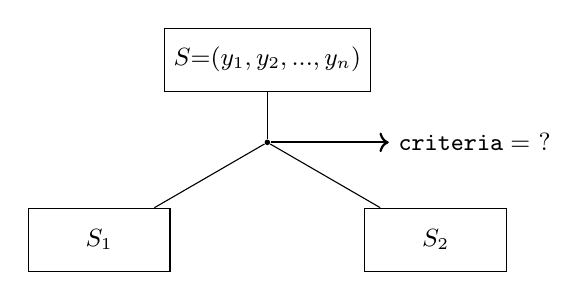
\begin{tikzpicture}[
    node distance=0.8cm,
    box/.style={rectangle, draw, minimum width=1.8cm, minimum height=0.8cm, text centered, font=\small},
    dot/.style={circle, fill=black, minimum size=2pt, inner sep=0pt},
    arrow/.style={->, thick}
]
% Main parent node
\node[box] (parent) {$S$=\\$(y_1, y_2, ..., y_n)$};
% Split point (dot in the middle)
\node[dot, below=0.6cm of parent] (split) {};
% Two child nodes
\node[box, below left=0.8cm and 1.2cm of split] (left) {$S_1$};
\node[box, below right=0.8cm and 1.2cm of split] (right) {$S_2$};
% Connections
\draw (parent) -- (split);
\draw (split) -- (left);
\draw (split) -- (right);
% Loss function arrow and equation
\node[right=1.5cm of split, font=\small] (loss) {$\texttt{criteria} = $ ?};
\draw[arrow] (split) -- (loss);
\end{tikzpicture}

\label{fig:decision_tree_split}
\end{figure}



    \end{column}
\begin{column}{0.6\linewidth}
\vspace{1cm}
$\qquad \qquad$A binary decision tree
\vspace

\resizebox{1\linewidth}{!}{%
        \begin{tikzpicture}[
  level/.style={sibling distance=60mm/#1},
  every node/.style={circle, draw, minimum size=8mm, font=\tiny},
  dots/.style={draw=none, font=\large}
]
\node {Root}
  child {
    node {L1}
    child {
      node {L2}
      child {
        node[dots] {$\vdots$}
      }
      child {
        node[dots] {$\vdots$}
      }
    }
    child {
      node {L2}
      child {
        node[dots] {$\vdots$}
      }
      child {
        node[dots] {$\vdots$}
      }
    }
  }
  child {
    node {R1}
    child {
      node {L2}
      child {
        node[dots] {$\vdots$}
      }
      child {
        node[dots] {$\vdots$}
      }
    }
    child {
      node {L2}
      child {
        node[dots] {$\vdots$}
      }
      child {
        node[dots] {$\vdots$}
      }
    }
  };
\end{tikzpicture}}
    \end{column}

    
\end{columns}


}

\end{frame}






\begin{frame}{}\only<1>{\frametitle{MSE splitting}
\note{Just for a very brief explanation: Let’s consider a node of a decision tree with \( n \) observations and \( m \) covariates. When we  want to split the data, we need a partition rule:

\begin{itemize}
  \item \textbf{First}, we need to decide which covariate, among the \( m \), should be used for the split.
  \item \textbf{Second}, we need to determine a split value, let’s call it \( c \).
\end{itemize}


}
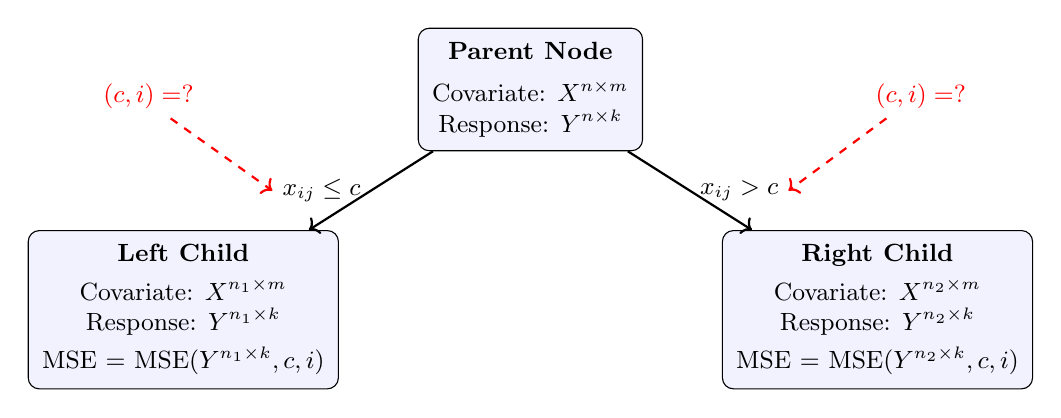
\begin{tikzpicture}[
  node distance=1cm and 1cm,
  every node/.style={font=\small},
  data/.style={rectangle, draw, align=center, fill=blue!5, rounded corners, inner sep=5pt},
  split/.style={->, thick},
  highlight/.style={->, red, thick, dashed}
  ]
  % Parent node
  \node[data] (parent) {
    \textbf{Parent Node} \\[0.15cm]
    Covariate: $X^{n \times m}$ \\ 
    Response: $Y^{n \times k}$
  };
  % Left child
  \node[data, below left=of parent] (left) {
    \textbf{Left Child} \\[0.1cm]
    Covariate: $X^{n_1 \times m}$ \\
    Response: $Y^{n_1 \times k}$ \\[0.1cm]
    MSE = $\text{MSE}(Y^{n_1 \times k},c,i)$
  };
  % Right child
  \node[data, below right=of parent] (right) {
    \textbf{Right Child} \\[0.1cm]
    Covariate: $X^{n_2 \times m}$ \\
    Response: $Y^{n_2 \times k}$ \\[0.1cm]
    MSE = $\text{MSE}(Y^{n_2 \times k},c,i)$
  };
  % Arrows
  \draw[split] (parent) -- node[midway, left] (leftlabel) {$x_{ij} \leq c$} (left);
  \draw[split] (parent) -- node[midway, right] (rightlabel) {$x_{ij} > c$} (right);
  
  % Optimize labels
  \node[red, left] (opt_i) at ([xshift=-1.5cm, yshift=1.2cm]leftlabel) {\textbf{ } $(c,i)=?$};
  \node[red, right] (opt_c) at ([xshift=1.5cm, yshift=1.2cm]rightlabel) {\textbf{} $(c,i)=?$};
  
  % Short highlight arrows from labels to split conditions
  \draw[highlight] (opt_i) -- (leftlabel.west);
  \draw[highlight] (opt_c) -- (rightlabel.east);
\end{tikzpicture}


}
\only<2>{
\note{For example, assume we choose a splitting rule based on covariate 2, and the split value is 3.1.

What we do is very simple. We go to the second column of the table, and for each observation:

if the value is less than 3.1, we assign it to the left node,
if the value is greater than or equal to 3.1, we assign it to the right node.


Now the main question is: how do we choose the best split? or what is the optimal partition rule?



And more importantly, what does “best” actually mean in this context?

This is exactly where the learning criterion comes in, and it defines how the tree grows.}
\frametitle{Split rule}
\begin{columns}[T]

  \column{0.8\textwidth}
 \begin{center}
\renewcommand{\arraystretch}{1.6}
\begin{tabular}{c|c>{\columncolor{purple!20}}cc>{\columncolor{purple!20}}cc|ccc|c}
\textbf{obs} & $x_1$ & \cellcolor{purple!50}$x_2$ & $x_3$ & \cellcolor{purple!20}$x_4$ & $x_5$ & $y_1$ & $y_2$ & $y_3$ & \textbf{child} \\
\hline
\rowcolor{blue!15}
1 & 0.8 & \textbf{1.2} & 3.4 & 0.5 & 2.1 & 0.60 & 0.25 & 0.15 & \textcolor{blue!80!black}{$\leftarrow$ left} \\
\rowcolor{blue!15}
2 & 2.3 & \textbf{2.7} & 1.1 & 4.2 & 0.9 & 0.10 & 0.70 & 0.20 & \textcolor{blue!80!black}{$\leftarrow$ left} \\
\rowcolor{blue!15}
3 & 1.5 & \textbf{3.1} & 2.9 & 1.8 & 3.3 & 0.45 & 0.45 & 0.10 & \textcolor{blue!80!black}{$\leftarrow$ left} \\
\rowcolor{red!15}
4 & 3.9 & \textbf{4.4} & 0.7 & 3.1 & 1.4 & 0.05 & 0.15 & 0.80 & \textcolor{red!80!black}{right $\rightarrow$} \\
\rowcolor{blue!15}
5 & 0.4 & \textbf{2.0} & 4.5 & 2.7 & 5.0 & 0.50 & 0.30 & 0.20 & \textcolor{blue!80!black}{$\leftarrow$ left} \\
\rowcolor{red!15}
6 & 2.1 & \textbf{5.6} & 3.8 & 0.3 & 2.2 & 0.02 & 0.08 & 0.90 & \textcolor{red!80!black}{right $\rightarrow$} \\
\rowcolor{red!15}
7 & 3.3 & \textbf{3.8} & 1.6 & 4.9 & 0.6 & 0.03 & 0.12 & 0.85 & \textcolor{red!80!black}{right $\rightarrow$} \\
\rowcolor{blue!15}
8 & 1.1 & \textbf{1.5} & 2.2 & 1.1 & 4.4 & 0.55 & 0.35 & 0.10 & \textcolor{blue!80!black}{$\leftarrow$ left} \\
\end{tabular}
\end{center}

  \column{0.22\textwidth}
  \vspace{1em}
  \begin{block}{Partition rule}
    Covariate 2: $i=2$ \\ Split value: $c =3.1$\\
    
  \end{block}
  \vspace{0.8em}
  \textcolor{blue!80!black}{\textbf{Left}} \\
  \hspace{0.5em} $x_2 \leq 3.1$ \\[0.2em]
  \hspace{0.5em} obs: 1, 2, 3, 5, 8 \\[0.6em]
  \textcolor{red!80!black}{\textbf{Right}} \\
   \hspace{0.5em} $x_2 > 3.1$ \\
  \hspace{0.5em} obs: 4, 6, 7


\end{columns}
}


\end{frame}




% %--- SLIDE 1: The data ---
% \begin{frame}{Growing a Tree: The Data}
% \begin{columns}[T]

%   \column{0.65\textwidth}
%   \begin{center}
%   \renewcommand{\arraystretch}{1.6}
%   \begin{tabular}{c|ccccc|ccc}
%   \textbf{obs} & $x_1$ & $x_2$ & $x_3$ & $x_4$ & $x_5$ & $y_1$ & $y_2$ & $y_3$ \\
%   \hline
%   1 & 0.8 & 1.2 & 3.4 & 0.5 & 2.1 & 0.60 & 0.25 & 0.15 \\
%   2 & 2.3 & 2.7 & 1.1 & 4.2 & 0.9 & 0.10 & 0.70 & 0.20 \\
%   3 & 1.5 & 3.1 & 2.9 & 1.8 & 3.3 & 0.45 & 0.45 & 0.10 \\
%   4 & 3.9 & 4.4 & 0.7 & 3.1 & 1.4 & 0.05 & 0.15 & 0.80 \\
%   5 & 0.4 & 2.0 & 4.5 & 2.7 & 5.0 & 0.50 & 0.30 & 0.20 \\
%   6 & 2.1 & 5.6 & 3.8 & 0.3 & 2.2 & 0.02 & 0.08 & 0.90 \\
%   7 & 3.3 & 3.8 & 1.6 & 4.9 & 0.6 & 0.03 & 0.12 & 0.85 \\
%   8 & 1.1 & 1.5 & 2.2 & 1.1 & 4.4 & 0.55 & 0.35 & 0.10 \\
%   \end{tabular}
%   \end{center}

%   \column{0.32\textwidth}
%   \vspace{1em}
%   \begin{block}{Setup}
%     Each node holds $n$ observations with $p$ covariates.
%   \end{block}
%   \vspace{0.8em}
%   \textbf{Response} $\mathbf{y}$ is compositional:
%   \[
%     \mathbf{y} = (y_1, y_2, y_3)
%   \]
%   \[
%     y_k \geq 0, \quad \textstyle\sum_k y_k = 1
%   \]
%   \vspace{0.4em}
%   Lives on the simplex $\mathcal{S}^2$.

% \end{columns}
% \end{frame}


% %--- SLIDE 2: Select covariates ---
% \begin{frame}{Step 1 — Select Covariates}
% \begin{columns}[T]

%   \column{0.65\textwidth}
%   \begin{center}
%   \renewcommand{\arraystretch}{1.6}
%   \begin{tabular}{c|c>{\columncolor{purple!20}}cc>{\columncolor{purple!20}}cc|ccc}
%   \textbf{obs} & $x_1$ & \cellcolor{purple!50}$x_2$ & $x_3$ & \cellcolor{purple!50}$x_4$ & $x_5$ & $y_1$ & $y_2$ & $y_3$ \\
%   \hline
%   1 & 0.8 & 1.2 & 3.4 & 0.5 & 2.1 & 0.60 & 0.25 & 0.15 \\
%   2 & 2.3 & 2.7 & 1.1 & 4.2 & 0.9 & 0.10 & 0.70 & 0.20 \\
%   3 & 1.5 & 3.1 & 2.9 & 1.8 & 3.3 & 0.45 & 0.45 & 0.10 \\
%   4 & 3.9 & 4.4 & 0.7 & 3.1 & 1.4 & 0.05 & 0.15 & 0.80 \\
%   5 & 0.4 & 2.0 & 4.5 & 2.7 & 5.0 & 0.50 & 0.30 & 0.20 \\
%   6 & 2.1 & 5.6 & 3.8 & 0.3 & 2.2 & 0.02 & 0.08 & 0.90 \\
%   7 & 3.3 & 3.8 & 1.6 & 4.9 & 0.6 & 0.03 & 0.12 & 0.85 \\
%   8 & 1.1 & 1.5 & 2.2 & 1.1 & 4.4 & 0.55 & 0.35 & 0.10 \\
%   \end{tabular}
%   \end{center}

%   \column{0.32\textwidth}
%   \vspace{1em}
%   \begin{block}{Random subspace}
%     At each node, draw $m \leq p$ covariates at random.
%   \end{block}
%   \vspace{0.8em}
%   \textcolor{purple!80!black}{\textbf{Selected:}} $x_2,\, x_4$
%   \vspace{0.6em}

%   \begin{itemize}[label={\ding{226}}]
%     \item Reduces correlation between trees
%     \item Only \textcolor{purple!80!black}{highlighted columns} are split candidates
%     \item Other columns are ignored at this node
%   \end{itemize}

% \end{columns}
% \end{frame}


% %--- SLIDE 3: Find the best split ---
% \begin{frame}{Step 2 — Find the Best Split}
% \begin{columns}[T]

%   \column{0.72\textwidth}
%   \begin{center}
%   \renewcommand{\arraystretch}{1.6}
%   \begin{tabular}{c|c>{\columncolor{purple!20}}cc>{\columncolor{purple!20}}cc|ccc|c}
%   \textbf{obs} & $x_1$ & \cellcolor{purple!50}$x_2$ & $x_3$ & \cellcolor{purple!20}$x_4$ & $x_5$ & $y_1$ & $y_2$ & $y_3$ & \\
%   \hline
%   \rowcolor{leftblue}
%   1 & 0.8 & \textbf{1.2} & 3.4 & 0.5 & 2.1 & 0.60 & 0.25 & 0.15 & \textcolor{blue!80!black}{$\leftarrow$ left} \\
%   \rowcolor{leftblue}
%   2 & 2.3 & \textbf{2.7} & 1.1 & 4.2 & 0.9 & 0.10 & 0.70 & 0.20 & \textcolor{blue!80!black}{$\leftarrow$ left} \\
%   \rowcolor{leftblue}
%   3 & 1.5 & \textbf{3.1} & 2.9 & 1.8 & 3.3 & 0.45 & 0.45 & 0.10 & \textcolor{blue!80!black}{$\leftarrow$ left} \\
%   \rowcolor{rightred}
%   4 & 3.9 & \textbf{4.4} & 0.7 & 3.1 & 1.4 & 0.05 & 0.15 & 0.80 & \textcolor{red!80!black}{right $\rightarrow$} \\
%   \rowcolor{leftblue}
%   5 & 0.4 & \textbf{2.0} & 4.5 & 2.7 & 5.0 & 0.50 & 0.30 & 0.20 & \textcolor{blue!80!black}{$\leftarrow$ left} \\
%   \rowcolor{rightred}
%   6 & 2.1 & \textbf{5.6} & 3.8 & 0.3 & 2.2 & 0.02 & 0.08 & 0.90 & \textcolor{red!80!black}{right $\rightarrow$} \\
%   \rowcolor{rightred}
%   7 & 3.3 & \textbf{3.8} & 1.6 & 4.9 & 0.6 & 0.03 & 0.12 & 0.85 & \textcolor{red!80!black}{right $\rightarrow$} \\
%   \rowcolor{leftblue}
%   8 & 1.1 & \textbf{1.5} & 2.2 & 1.1 & 4.4 & 0.55 & 0.35 & 0.10 & \textcolor{blue!80!black}{$\leftarrow$ left} \\
%   \end{tabular}
%   \end{center}

%   \column{0.25\textwidth}
%   \vspace{1em}
%   \begin{block}{Partition rule}
%     \textcolor{purple!80!black}{Best:} $x_2 \leq 3.5$
%   \end{block}
%   \vspace{0.8em}
%   \textcolor{blue!80!black}{\textbf{Left}} \hfill $x_2 \leq 3.5$\\[0.2em]
%   \hspace{0.5em} obs: 1,2,3,5,8 \\[0.6em]
%   \textcolor{red!80!black}{\textbf{Right}} \hfill $x_2 > 3.5$ \\[0.2em]
%   \hspace{0.5em} obs: 4,6,7
%   \vspace{0.6em}



% \end{columns}
% \end{frame}





\begin{frame}{}\only<1>{\frametitle{MSE splitting}
\note{Just for a very brief explanation: Let’s consider a node of a decision tree with \( n \) observations and \( m \) covariates. When we  want to split the data, we face two key decisions:

\begin{itemize}
  \item \textbf{First}, we need to decide which covariate, among the \( m \), should be used for the split.
  \item \textbf{Second}, we need to determine a split value, let’s call it \( c \).
\end{itemize}


So, the problem is to find the optimal pair \( (i, c) \).  For regression trees, the usual splitting criterion is the mean squared error (MSE). 

The mean squared error (MSE) does not account for the simplex constraint.
}
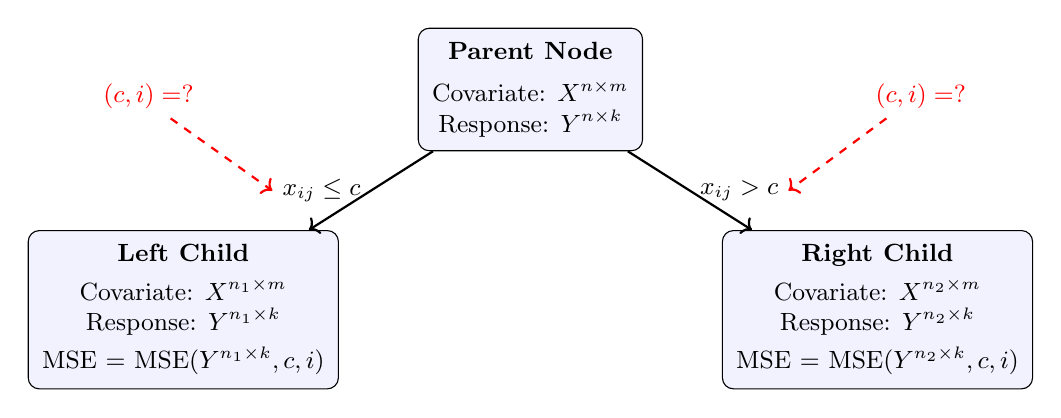
\begin{tikzpicture}[
  node distance=1cm and 1cm,
  every node/.style={font=\small},
  data/.style={rectangle, draw, align=center, fill=blue!5, rounded corners, inner sep=5pt},
  split/.style={->, thick},
  highlight/.style={->, red, thick, dashed}
  ]
  % Parent node
  \node[data] (parent) {
    \textbf{Parent Node} \\[0.15cm]
    Covariate: $X^{n \times m}$ \\ 
    Response: $Y^{n \times k}$
  };
  % Left child
  \node[data, below left=of parent] (left) {
    \textbf{Left Child} \\[0.1cm]
    Covariate: $X^{n_1 \times m}$ \\
    Response: $Y^{n_1 \times k}$ \\[0.1cm]
    MSE = $\text{MSE}(Y^{n_1 \times k},c,i)$
  };
  % Right child
  \node[data, below right=of parent] (right) {
    \textbf{Right Child} \\[0.1cm]
    Covariate: $X^{n_2 \times m}$ \\
    Response: $Y^{n_2 \times k}$ \\[0.1cm]
    MSE = $\text{MSE}(Y^{n_2 \times k},c,i)$
  };
  % Arrows
  \draw[split] (parent) -- node[midway, left] (leftlabel) {$x_{ij} \leq c$} (left);
  \draw[split] (parent) -- node[midway, right] (rightlabel) {$x_{ij} > c$} (right);
  
  % Optimize labels
  \node[red, left] (opt_i) at ([xshift=-1.5cm, yshift=1.2cm]leftlabel) {\textbf{ } $(c,i)=?$};
  \node[red, right] (opt_c) at ([xshift=1.5cm, yshift=1.2cm]rightlabel) {\textbf{} $(c,i)=?$};
  
  % Short highlight arrows from labels to split conditions
  \draw[highlight] (opt_i) -- (leftlabel.west);
  \draw[highlight] (opt_c) -- (rightlabel.east);
\end{tikzpicture}

\begin{equation*}
    
(c^*, i^*) 
&=& \operatorname{argmin}_{i,c} \left( \text{MSE}(Y^{n_1 \times k},c,i) + \text{MSE}(Y^{n_2 \times k},c,i) \right)
\\
&=& \arg\min_{c,j} 
\left\{\frac{n_1(c,j)}{n}
\sum_{m=1}^k \sum_{i=1}^{n_1(c,j)} (y_{im}-\bar{y}_{m}^{n_1(c,j)})^2
+
\frac{n_2(c,j)}{n}
\sum_{m=1}^k \sum_{i=1}^{n_2(c,j)} (y_{im}-\bar{y}_{m}^{n_2(c,j)})^2
\right\}.
\end{equation*}

}



\only<2>{ \frametitle{MSE splitting}
\note{ But using mse has a problem, which is that in simplex space, the component variance usually depends on E. for example, if the outcome variable follows a Dirichlet distribution, obviously the variance depends on the mean parameter \(\mu\). This is a violation of the homoscedasticity assumption.

One possible idea is to use maximum likelihood instead of distance measures. In this approach, each node is split into two child nodes in a way that gives the best overall likelihood.

To solve this, we use the total \textbf{log-likelihood} under the Dirichlet distribution.


}
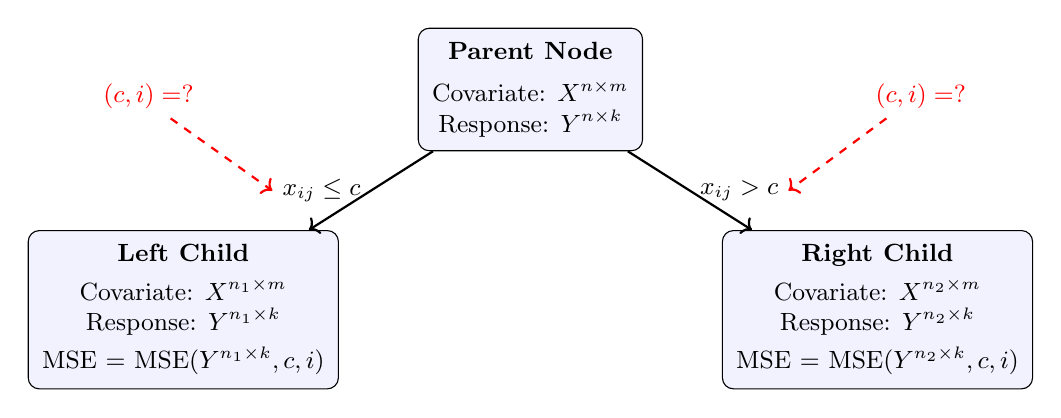
\begin{tikzpicture}[
  node distance=1cm and 1cm,
  every node/.style={font=\small},
  data/.style={rectangle, draw, align=center, fill=blue!5, rounded corners, inner sep=5pt},
  split/.style={->, thick},
  highlight/.style={->, red, thick, dashed}
  ]
  % Parent node
  \node[data] (parent) {
    \textbf{Parent Node} \\[0.15cm]
    Covariate: $X^{n \times m}$ \\ 
    Response: $Y^{n \times k}$
  };
  % Left child
  \node[data, below left=of parent] (left) {
    \textbf{Left Child} \\[0.1cm]
    Covariate: $X^{n_1 \times m}$ \\
    Response: $Y^{n_1 \times k}$ \\[0.1cm]
    MSE = $\text{MSE}(Y^{n_1 \times k},c,i)$
  };
  % Right child
  \node[data, below right=of parent] (right) {
    \textbf{Right Child} \\[0.1cm]
    Covariate: $X^{n_2 \times m}$ \\
    Response: $Y^{n_2 \times k}$ \\[0.1cm]
    MSE = $\text{MSE}(Y^{n_2 \times k},c,i)$
  };
  % Arrows
  \draw[split] (parent) -- node[midway, left] (leftlabel) {$x_{ij} \leq c$} (left);
  \draw[split] (parent) -- node[midway, right] (rightlabel) {$x_{ij} > c$} (right);
  
  % Optimize labels
  \node[red, left] (opt_i) at ([xshift=-1.5cm, yshift=1.2cm]leftlabel) {\textbf{ } $(c,i)=?$};
  \node[red, right] (opt_c) at ([xshift=1.5cm, yshift=1.2cm]rightlabel) {\textbf{} $(c,i)=?$};
  
  % Short highlight arrows from labels to split conditions
  \draw[highlight] (opt_i) -- (leftlabel.west);
  \draw[highlight] (opt_c) -- (rightlabel.east);
\end{tikzpicture}
\begin{itemize}
    \item 
MSE does not account for the simplex constraint.

\item 
\[V(X_i)=\frac{E(X_i)\left(1-E(X_i)\right)}{\alpha_0+1}\]
\end{itemize}

}

\end{frame}







\begin{frame}
\only<1>{
\frametitle{Dirichlet distribution}
\note{The only familiar class of distributions on simplex space is dirichlet distribution. This model operates directly on the simplex without requiring the data to be transformed into another space.

Other distributions have also been developed for compositional data, but most of them are based on transformations. In this work, we use the Dirichlet distribution.
}


\vspace{1em}

\begin{center}
\colorbox{green!10}{\parbox{0.95\textwidth}{
\begin{center}
\resizebox{\linewidth}{!}{%
\[
    f_{\mathbf{Z}}((z_1,\ldots,z_k); \boldsymbol{\alpha}) = \frac{\Gamma( \alpha_0)}{\prod_{i=1}^k \Gamma(\alpha_i)} \prod_{i=1}^k z_i^{\alpha_i - 1},
\quad  z_i \in [0, 1], \quad \sum_{i=1}^k z_i = 1,
\]
}
\end{center}
}}
\end{center}

\vspace{1.5em}

\begin{itemize}[itemsep=0.8em]


\item[\textcolor{blue}{\large$\blacktriangleright$}] The sum-constant requirement of the simplex is satisfied under the Dirichlet distribution.

\item[\textcolor{blue}{\large$\blacktriangleright$}] \textbf{Extensions available:} Zero-inflated Dirichlet and Kummer–Dirichlet
\end{itemize}
}

\end{frame}


\begin{frame}
\only<1>{\frametitle{Dirichlet log-likelihood splitting}
\note{



\vspace{1em}
We approach this optimization by maximizing the total log-likelihood. Specifically, for each candidate split \( (i, c) \), we compute the log-likelihoods of the two resulting sub-nodes, sum them, and identify the pair \( (i, c) \) that yields the highest total log-likelihood.

\vspace{1em}
The remaining steps follow the standard decision tree procedure.

\vspace{1em}
With this modification, we obtain a random forest—referred to as the \textbf{Dirichlet Random Forest}—which can be applied directly to compositional data, without requiring transformation.


}
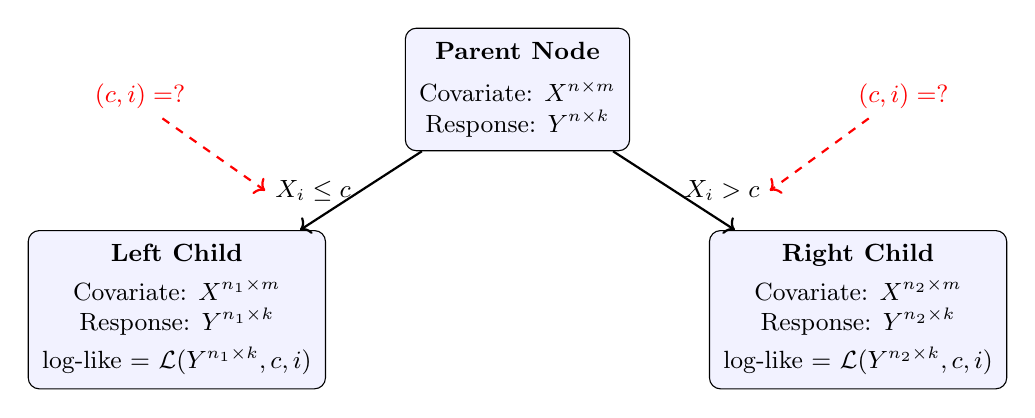
\begin{tikzpicture}[
  node distance=1cm and 1cm,
  every node/.style={font=\small},
  data/.style={rectangle, draw, align=center, fill=blue!5, rounded corners, inner sep=5pt},
  split/.style={->, thick},
  highlight/.style={->, red, thick, dashed}
  ]
  % Parent node
  \node[data] (parent) {
    \textbf{Parent Node} \\[0.15cm]
    Covariate: $X^{n \times m}$ \\ 
    Response: $Y^{n \times k}$
  };
  % Left child
  \node[data, below left=of parent] (left) {
    \textbf{Left Child} \\[0.1cm]
    Covariate: $X^{n_1 \times m}$ \\
    Response: $Y^{n_1 \times k}$ \\[0.1cm]
     log-like = $\mathcal{L}(Y^{n_1 \times k},c,i)$
  };
  % Right child
  \node[data, below right=of parent] (right) {
    \textbf{Right Child} \\[0.1cm]
    Covariate: $X^{n_2 \times m}$ \\
    Response: $Y^{n_2 \times k}$ \\[0.1cm]
     log-like = $\mathcal{L}(Y^{n_2 \times k},c,i)$
  };
  % Arrows
  \draw[split] (parent) -- node[midway, left] (leftlabel) {$X_{i} \leq c$} (left);
  \draw[split] (parent) -- node[midway, right] (rightlabel) {$X_{i} > c$} (right);
  
  % Optimize labels
  \node[red, left] (opt_i) at ([xshift=-1.5cm, yshift=1.2cm]leftlabel) {\textbf{ } $(c,i)=?$};
  \node[red, right] (opt_c) at ([xshift=1.5cm, yshift=1.2cm]rightlabel) {\textbf{} $(c,i)=?$};
  
  % Short highlight arrows from labels to split conditions
  \draw[highlight] (opt_i) -- (leftlabel.west);
  \draw[highlight] (opt_c) -- (rightlabel.east);
\end{tikzpicture}
\[
(c^*, i^*) = \operatorname{argmax}_{i,c} \left( \max_{\boldsymbol{\alpha}} \mathcal{L}(Y^{n_1 \times k},c,i) + \max_{\boldsymbol{\alpha}} \mathcal{L}(Y^{n_2 \times k},c,i) \right)
\]
}
\end{frame}

\begin{frame}{Prediction based on DirichletRF}
\note{
    By considering the Dirichlet distribution, we eventually obtain several terminal nodes, each containing a set of observations. For a new observation, we traverse the decision tree to identify the corresponding terminal node. 

    default: 
    
    In a regression decision tree, we then have two options for prediction: either use the mean of the observations in that node, or use the estimated parameters of the Dirichlet distribution as the prediction.

    In a random forest, we repeat this process for many trees and finally take the mean of the predictions from all the trees.

    another idea:
    
Then, in that terminal node, we have a set of observations.

In a random forest, we repeat this process for many trees, and in the end we obtain several terminal nodes, each one associated with a different tree. We use these observations to construct an empirical probability function.

    }
    
\begin{columns}[T]

% Left column - Graph
\begin{column}{0.45\textwidth}
\centering
\begin{tikzpicture}[
    node/.style={ellipse, draw, minimum width=1.2cm, minimum height=0.8cm, thick},
    leaf/.style={rectangle, draw, minimum width=1.8cm, minimum height=0.6cm, thick},
    arrow/.style={->, thick, blue},
    scale=0.75,
    every node/.style={transform shape}
]

% Root node
\node[node] (root) at (0,0) {};

% Level 1
\node[node] (n1) at (-2,-2) {};
\node (dots1) at (1,-2) {\vdots};

% Level 2
\node (dots2) at (-3,-3.5) {\vdots};
\node[node] (n2) at (-1,-4) {};

% Level 3
\node (dots3) at (-2.5,-5.5) {\vdots};
\node[node] (n3) at (0,-6) {};

% Level 4
\node (dots4) at (1,-7.5) {\vdots};
\node[leaf] (leaf) at (-1,-8) {$\{y_1, y_2, \ldots, y_n\}$};

% Arrows - traversal path highlighted
\draw[arrow, line width=1.5pt] (root) -- (n1);
\draw[arrow, dashed] (root) -- (dots1);
\draw[arrow, dashed] (n1) -- (dots2);
\draw[arrow, line width=1.5pt] (n1) -- (n2);
\draw[arrow, dashed] (n2) -- (dots3);
\draw[arrow, line width=1.5pt] (n2) -- (n3);
\draw[arrow, line width=1.5pt] (n3) -- (leaf);
\draw[arrow, dashed] (n3) -- (dots4);

\end{tikzpicture}
\end{column}

% Right column - Explanation
\begin{column}{0.52\textwidth}
\small

\textbf{Process:}
\begin{itemize}[label=\arabic*.]
    \item Start at root node
    \item Traverse tree based on decision rules
    \item Reach terminal node with observations
\end{itemize}

\vspace{0.4cm}

\textbf{Default Approach:}
\begin{itemize}
    \item Mean: $\hat{y} = \frac{1}{n}\sum_{i=1}^{n} y_i$
    \item Expectation: $\text{E}(Y_i) = \frac{\hat{\alpha}_i}{\sum_{j+1}^k\hat{\alpha}_i}$
    \item Random Forest: average across trees
\end{itemize}

\vspace{0.4cm}

\textbf{Distributional Approach:}
\begin{itemize}
    \item Collect terminal nodes from all trees
    \item Construct empirical probability function
\end{itemize}

\end{column}

\end{columns}

\end{frame}












% %\begin{frame}{Comparison Results}
      \centering
      \vfill
      \textbf{\Large Comparison Results}
      \vfill
\end{frame}

\begin{frame}{Performance Evaluation and Transformations}

To evaluate DirichletRF's performance, we compare it with two alternative approaches:
\begin{itemize}
    \item[1)] \textbf{ILR-RF:} A Random Forest model based on log-ratio transformations. 
    The compositional data are first transformed into the ILR
    space. Then, a standard Random Forest is applied to the transformed data, and 
    finally, the predictions are mapped back to the simplex for interpretation.

    \item[2)] \textbf{Dirichlet Regression:} A parametric approach that, 
    works directly on the simplex without requiring any transformation.
\end{itemize}

\end{frame}




\begin{frame}{Evaluation Metrics}
\note{
To compare these models, we used  the Aitchison Distance and the Root Mean Square Error, or RMSE.

The Aitchison Distance is the usual Euclidean distance between them.

On the other hand, RMSE is a widely used and well-known metric. Unlike the Aitchison Distance, it does not take into account the geometric structure of the simplex
}
To compare these models, we used  the Aitchison Distance and the Root Mean Square Error, or RMSE.
\vspace{0.2cm}
\textbf{1. Aitchison Distance:}
\[
AC = \frac{1}{n} \sum_{i=1}^n \sqrt{\sum_{j=1}^k \left(\log\frac{Y_{ij}}{g(\mathbf{Y}_i)} - \log\frac{\hat{Y}_{ij}}{g(\hat{\mathbf{Y}}_i)}\right)^2},
\]
\[
\text{where} \quad g(\mathbf{Y}_i) = \left(\prod_{j=1}^k Y_{ij}\right)^{1/k}
\]
\textit{Measures compositional dissimilarity using log-ratio geometry.}

\vspace{0.3cm}
\textbf{2. Root Mean Square Error (RMSE):}
$
\text{RMSE}_k =  \sqrt{\frac{1}{n} \sum_{i=1}^n (Y_{ij} - \hat{Y}_{ij})^2}
$

\vspace{0.3cm}
\textbf{Interpretation:} Lower values for both metrics indicate better predictive accuracy.
\end{frame}








\begin{frame}{}

    \only<1>{
    \note{We generated two datasets — one simple and one more complex. Here, we used three covariates and a three-dimensional compositional response. The response data was generated from a Dirichlet distribution with a simple, linear relationship to the covariates.}
    \textbf{Simple structure simulations}: We use a simple dataset with $3$ Covariate variables, $X_1,X_1, X_{3}$ and with a $3$-dimensional response, $(Y_1,\,Y_2,\,Y_3)$ such that $Y_1+Y_2+Y_3 = 1$. The response is assumed to follow a Dirichlet distribution with the following parameters:
\[
\alpha_1 = 1 + 2 X_1,\quad \alpha_2 =1 + 0.5 X_2,\quad \alpha_3 = 1 + X_3.
\]
\[
(Y_1,\,Y_2,\,Y_3)\sim Dirichlet(\alpha_1,\alpha_2,\alpha_3)
\]
    }
    \only<2>{
    \note{In this table, you can see the results for the this dataset across different sample sizes.
The first and second columns show the performance of each model based on the both metrics measured on the test set.
The last column shows the difference between the Aitchison Distance on the test and train datasets, which gives us insight into overfitting.

Dirichlet Regression performed better than the other models. This result makes sense, because the data was generated using a Dirichlet distribution with a linear structure.

But, Dirichlet Random Forest does not perform well in this case — in fact, it gives the worst performance in terms of Aitchison Distance and RMSE.

It just performs better than CLR-RF and ILR-RF when it comes to overfitting.

So, we can say that in this example, the main advantage of Dirichlet Random Forest compared to the other RF models is that it is more robust against overfitting.}
    
\begin{table}[htbp]
\centering
\small 
\begin{tabular}{|l|l|c|c|c|c|}
\hline
$N$ & Model & Aitchison Distance  & RMSE & Train-Test \\
\hline

{200} 
    & CLR-RF & 1.299 (0.141) & 0.703 (0.039) & 0.684 \\
    & ILR-RF & 1.303 (0.143) & 0.700 (0.040)& 0.686 \\
    & \textcolor{blue}{Dirichlet Regression} & \textcolor{blue}{\textbf{1.233} (0.139)} & \textcolor{blue}{\textbf{0.745} (0.033)}  & \textcolor{blue}{\textbf{0.030}} \\
    & \texttt{Dirichlet-RF} & 1.451 (0.153) & 0.620 (0.052)  & 0.600 \\
\hline
{500}
    & CLR-RF & 1.282 (0.077) & 0.716 (0.019)  & 0.684 \\
    & ILR-RF & 1.284 (0.077) & 0.716 (0.020)& 0.685 \\
    & \textcolor{blue}{Dirichlet Regression} & \textcolor{blue}{\textbf{1.234} (0.078)} & \textcolor{blue}{\textbf{0.752} (0.016)}  & \textcolor{blue}{\textbf{0.035}} \\
    & \texttt{Dirichlet-RF} & 1.450 (0.077) & 0.627 (0.031) & 0.616 \\
\hline
{2000}
    & CLR-RF & 1.249 (0.032) & 0.726 (0.010) & 0.652 \\
    & ILR-RF & 1.252 (0.032) & 0.725 (0.010)  & 0.654 \\
    & \textcolor{blue}{Dirichlet Regression} & \textcolor{blue}{\textbf{1.209} (0.032)} & \textcolor{blue}{\textbf{0.757} (0.008)}  & \textcolor{blue}{\textbf{0.006}} \\
    & \texttt{Dirichlet-RF} & 1.431 (0.041) & 0.635 (0.016) & 0.596 \\
\hline
\end{tabular}
\caption{ Values represent the means and (standard deviations) of the metrics for test datasets. Train-Test Diff represents the absolute difference between train and test Aitchison Distance, indicating model generalisation capability. }
\label{tab:performance-comparison1}
\end{table}}

    \only<3>{
    	    
    \note{
We compared these models on various datasets—both simulated and real-world. The performance comparison showed competitive results among the random forest-based models. Sometimes the Dirichlet Random Forest performed best, sometimes not—but it consistently delivered satisfactory outcomes.
One situation where it outperformed the others was when the structure of the dataset was complex. For example,
  consider three-dimensional compositional responses and with 10 covariates — only 3 of them are informative, and the other 7 have no relationship with the response. 
As you can see, the responses are generated from a normal distribution, and the relationship with the three informative covariates is nonlinear — we used functions like sin(x), exp(x), quantile, and other nonlinear forms.


    }
    Complex structure synthetic simulations: The dataset consisted of 10 predictor variables \((X_1, \ldots, X_{10})\), with only the first three variables \((X_1, X_2, X_3)\) being truly informative for predicting the compositional response. The three-component compositional response vector $\mathbf{Y} = (Y_1,Y_2,Y_3)$ was constructed through complex non-linear transformations of the informative Covariates. }
    \end{frame}
\begin{frame}
    \only<1>{

\begin{columns}
\begin{column}{0.5\linewidth}

% where \( \mathcal{N}(\mu_i, 0.5^2) \) represents a normally distributed random variable with mean \( \mu_i \) and standard deviation \( 0.5 \), and \( \epsilon \) is a small positive constant ensuring non-negativity.  
% The compositional response variables \( Y_1, Y_2, Y_3 \) are then obtained via the normalisation:
We generate the variables \( Z_1, Z_2, Z_3 \) as follows:  
\[
Z_i = \max(\epsilon, \mathcal{N}(\mu_i, 0.5)), \quad 
\]
\[
Y_i = \frac{Z_i}{Z_1 + Z_2 + Z_3}, \quad  i = 1,2,3.
\]
% This transformation ensures that \( (Y_1, Y_2, Y_3) \) lies within the unit simplex, preserving the compositional structure of the data.
\end{column}
		\begin{column}{0.5\linewidth}

\begin{align*}
\mu_{1j} &= g(2(1 + \sin(x_{1j}))+x_{2j}^3) \\
\mu_{2j} &= g(1 + 2.5\exp(x_{3j})+x_{1j}^2) \\
\mu_{3j} &= g(1 + (1+x_{2j})^2+x_{3j}^4)
\end{align*}

\end{column}

\end{columns}

Where
\[
g(x_{ij}) =
\begin{cases} 
    2, & x_{ij} < \text{Quantile}(x_i, 0.3) \\
    3, & \text{Quantile}(x_i, 0.3) \leq x_{ij} <\text{Quantile}(x_i, 0.6) \\
    4, & \text{Quantile}(x, 0.6) \leq x_{ij} \leq \text{Quantile}(x_i, 0.8) \\
    1, & x_i > \text{Quantile}(x_i, 0.8)
\end{cases}
\]

}
\end{frame}
\begin{frame}
\only<1>{
\note{In this complex scenario, the results are reversed. Our Dirichlet-RF is now the best model, and Dirichlet Regression is the worst.

In terms of overfitting, Dirichlet Regression still performs the best. But this is expected — we don’t usually expect a random forest model to outperform a parametric model with a simple structure when it comes to overfitting.
However, Dirichlet-RF still performs better than the other two random forest models. Overfitting is a common issue in decision tree-based models, but based on our experience, Dirichlet-RF shows better generalization and less overfitting.
}
\begin{table}[htbp]
\centering
\small 
\begin{tabular}{|l|l|c|c|c|c|}
\hline
N & Model & Aitchison Distance & RMSE & Train-Test \\

\hline
{200} 
    & CLR-RF & 0.671 (0.152) & 0.898 (0.018) & 0.366 \\
    & ILR-RF & 0.670 (0.151) & 0.899 (0.018) & 0.364 \\
    & Dirichlet Regression & 0.826 (0.155) & 0.844 (0.026)  & 0.068 \\
    & \textcolor{blue}{{Dirichlet-RF}} & \textcolor{blue}{\textbf{0.659} (0.152)} & \textcolor{blue}{\textbf{0.903} (0.017)}  & 0.221 \\
\hline
{500} 
    & CLR-RF & 0.617 (0.072) & 0.912 (0.011) &   0.334 \\
    & ILR-RF & 0.618 (0.072) & 0.911 (0.012) &  0.334 \\
    & Dirichlet Regression & 0.790 (0.075) & 0.855 (0.012)  & 0.029 \\
    & \textcolor{blue}{{Dirichlet-RF}} & \textcolor{blue}{\textbf{0.606} (0.068)} & \textcolor{blue}{\textbf{0.917} (0.010)}  & 0.201 \\
\hline
{2000} 
    & CLR-RF & 0.557 (0.045) & 0.931 (0.006) & 0.302 \\
    & ILR-RF & 0.557 (0.044) & 0.931 (0.006)& 0.301 \\
    & Dirichlet Regression & 0.785 (0.044) & 0.858 (0.006)  & 0.016\\
    &\textcolor{blue}{ {Dirichlet-RF}} & \textcolor{blue}{\textbf{0.544} (0.044)} & \textcolor{blue}{\textbf{0.936} (0.004) }& 0.178 \\
\hline
\end{tabular}
\caption{ Train-Test Diff represents the absolute difference between train and test Aitchison Distance.}
\label{tab:performance-comparison}
\end{table}
}
\only<2>{
\note{In this complex scenario, the results are reversed. Our Dirichlet-RF is now the best model, and Dirichlet Regression is the worst.

In terms of overfitting, Dirichlet Regression still performs the best. But this is expected — we don’t usually expect a random forest model to outperform a parametric model with a simple structure when it comes to overfitting.
However, Dirichlet-RF still performs better than the other two random forest models. Overfitting is a common issue in decision tree-based models, but based on our experience, Dirichlet-RF shows better generalization and less overfitting.
}
\begin{table}[htbp]
\centering
\small 
\begin{tabular}{|l|l|c|c|c|c|}
\hline
N & Model & Aitchison Distance & RMSE & Train-Test \\

\hline
{200} 
    & CLR-RF & 0.671 (0.152) & 0.898 (0.018) & 0.366 \\
    & ILR-RF & 0.670 (0.151) & 0.899 (0.018) & 0.364 \\
    & Dirichlet Regression & 0.826 (0.155) & 0.844 (0.026)  & \textcolor{blue}{\textbf{0.068}} \\
    & \textcolor{blue}{{Dirichlet-RF}} & 0.659 (0.152) & 0.903 (0.017)  & 0.221 \\
\hline
{500} 
    & CLR-RF & 0.617 (0.072) & 0.912 (0.011) &   0.334 \\
    & ILR-RF & 0.618 (0.072) & 0.911 (0.012) &  0.334 \\
    & Dirichlet Regression & 0.790 (0.075) & 0.855 (0.012)  & \textcolor{blue}{\textbf{0.029}} \\
    & \textcolor{blue}{{Dirichlet-RF}} & 0.606 (0.068) & 0.917 (0.010)  & 0.201 \\
\hline
{2000} 
    & CLR-RF & 0.557 (0.045) & 0.931 (0.006) & 0.302 \\
    & ILR-RF & 0.557 (0.044) & 0.931 (0.006)& 0.301 \\
    & Dirichlet Regression & 0.785 (0.044) & 0.858 (0.006)  & \textcolor{blue}{\textbf{0.016} }\\
    &\textcolor{blue}{ {Dirichlet-RF}} & 0.544 (0.044) & 0.936 (0.004) & 0.178 \\
\hline
\end{tabular}
\caption{ Train-Test Diff represents the absolute difference between train and test Aitchison Distance.}
\label{tab:performance-comparison}
\end{table}
}

\only<3>{
\note{In this complex scenario, the results are reversed. Our Dirichlet-RF is now the best model, and Dirichlet Regression is the worst.

In terms of overfitting, Dirichlet Regression still performs the best. But this is expected — we don’t usually expect a random forest model to outperform a parametric model with a simple structure when it comes to overfitting.
However, Dirichlet-RF still performs better than the other two random forest models. Overfitting is a common issue in decision tree-based models, but based on our experience, Dirichlet-RF shows better generalization and less overfitting.
}
\begin{table}[htbp]
\centering
\small 
\begin{tabular}{|l|l|c|c|c|c|}
\hline
N & Model & Aitchison Distance & RMSE & Train-Test \\

\hline
{200} 
    & CLR-RF & 0.671 (0.152) & 0.898 (0.018) & 0.366 \\
    & ILR-RF & 0.670 (0.151) & 0.899 (0.018) & 0.364 \\
    & Dirichlet Regression & 0.826 (0.155) & 0.844 (0.026)  & 0.068 \\
    & \textcolor{blue}{{Dirichlet-RF}} & 0.659 (0.152) & 0.903 (0.017)  & \textcolor{blue}{ \textbf{0.221}} \\
\hline
{500} 
    & CLR-RF & 0.617 (0.072) & 0.912 (0.011) &   0.334 \\
    & ILR-RF & 0.618 (0.072) & 0.911 (0.012) &  0.334 \\
    & Dirichlet Regression & 0.790 (0.075) & 0.855 (0.012)  & 0.029 \\
    & \textcolor{blue}{{Dirichlet-RF}} & 0.606 (0.068) & 0.917 (0.010)  & \textcolor{blue}{ \textbf{0.201}} \\
\hline
{2000} 
    & CLR-RF & 0.557 (0.045) & 0.931 (0.006) & 0.302 \\
    & ILR-RF & 0.557 (0.044) & 0.931 (0.006)& 0.301 \\
    & Dirichlet Regression & 0.785 (0.044) & 0.858 (0.006)  & 0.016\\
    &\textcolor{blue}{ {Dirichlet-RF}} & 0.544 (0.044) & 0.936 (0.004) & \textcolor{blue}{ \textbf{0.178}} \\
\hline
\end{tabular}
\caption{ Train-Test Diff represents the absolute difference between train and test Aitchison Distance.}
\label{tab:performance-comparison}
\end{table}
}
\end{frame}

\begin{frame}{Learning Curve}
\only<1>{


\begin{figure}
    \centering
    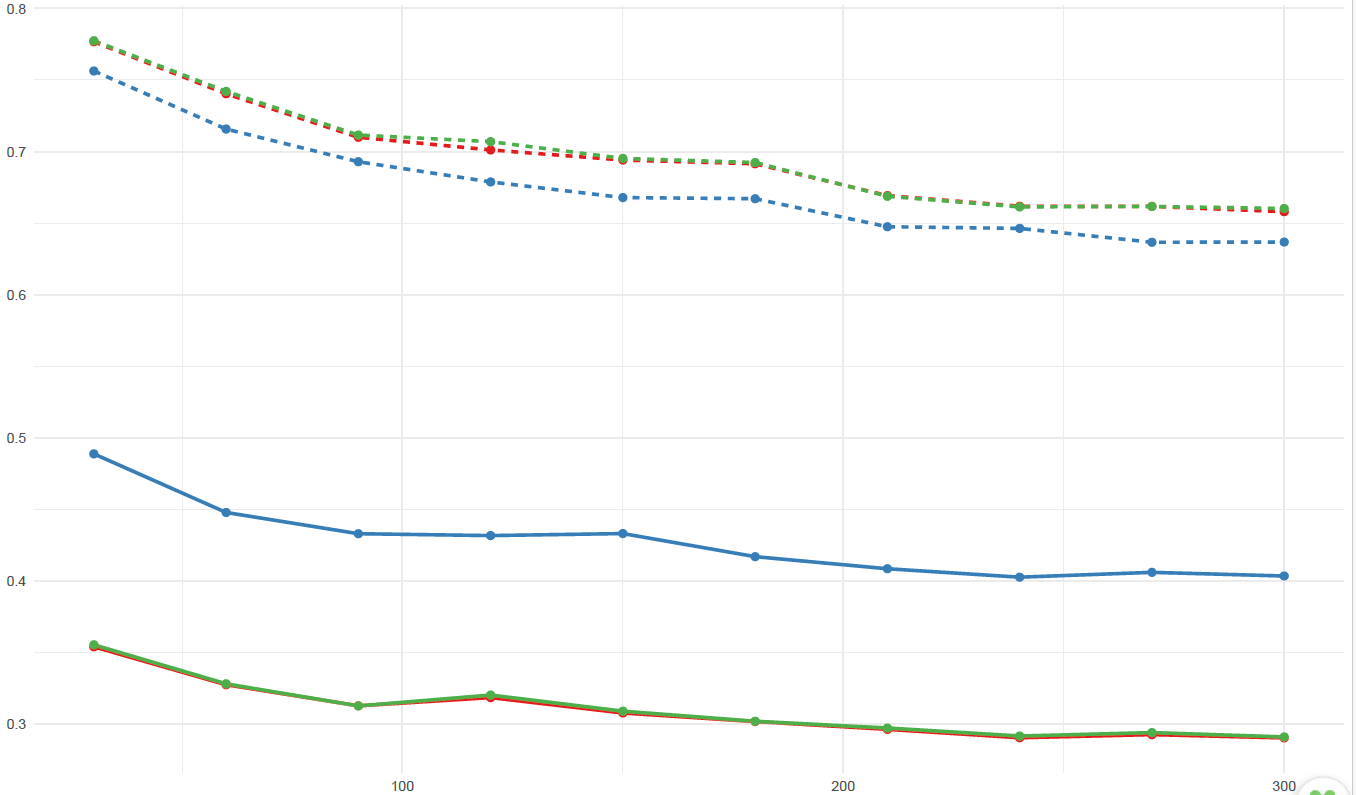
\includegraphics[width=0.75\linewidth]{Learning_curve.png}
    \caption{Aitchison distance as a function of training sample size for all three 
    Random Forest models.}
    \label{fig:enter-label}
\end{figure}
}
\end{frame}



\begin{frame}
\only<1>{
\note{I am not sure to include this slide:

And for further evaluation of \texttt{Dirichlet-RF}, we also looked at its performance in terms of covariate selection.

Here, you can see how often each covariate was selected for splitting across all trees, and how much, on average, it contributed to increasing the log-likelihood.

As I mentioned earlier, only three of the variables were informative — and \texttt{Dirichlet-RF} was able to clearly identify them with high importance.}
\begin{table}[htbp]
\centering
\begin{tabular}{|c|c|c|}
\hline
\textbf{Covariate} & \small{Log-Likelihood Importance} & \small{Frequency-Based Importance} \\
\hline
\textcolor{blue}{$X_1$} & \textcolor{blue}{225.039} & \textcolor{blue}{14} \\
\textcolor{blue}{$X_2$} & \textcolor{blue}{303.618} & \textcolor{blue}{21} \\
\textcolor{blue}{$X_3$} & \textcolor{blue}{272.036} & \textcolor{blue}{19} \\
\textcolor{red}{$X_4$} & \textcolor{red}{16.839}  & \textcolor{red}{2}  \\
\textcolor{red}{$X_5$} & \textcolor{red}{9.972}   & \textcolor{red}{2}  \\
\textcolor{red}{$X_6$} & \textcolor{red}{15.649}  & \textcolor{red}{3}  \\
\textcolor{red}{$X_7$} & \textcolor{red}{0}   & \textcolor{red}{0}  \\
\textcolor{red}{$X_8$} & \textcolor{red}{40.240}  & \textcolor{red}{6}  \\
\textcolor{red}{$X_9$} & \textcolor{red}{5.369}   & \textcolor{red}{1}  \\
\textcolor{red}{$X_{10}$} & \textcolor{red}{23.295}  & \textcolor{red}{3}  \\
\hline
\end{tabular}
\caption{Variable importance scores based on log-likelihood improvement and selection frequency, averaged across all trees in the \texttt{Dirichlet-RF}.}

\label{tab:variable-importance}
\end{table}
\note{
A noteworthy observation is that our model demonstrates effective Covariate selection capabilities through two complementary variable importance measures: log-likelihood importance, which quantifies each variable's contribution to model fit improvement, and frequency-based importance, which measures how often each variable is selected for splitting nodes. Both metrics are averaged across all trees in the random forest. Analysis shows that $X_1$, $X_2$, and $X_3$ receive the highest importance scores across both metrics, identifying them as the informative predictors in our simulation. The remaining variables ($X_4$ through $X_{10}$) receive substantially lower importance scores, confirming the model's ability to distinguish signal from noise.}
}
\end{frame}



\begin{frame}

    \only<1>{
  \note{This real-world dataset is based on a soil texture dataset from KwaZulu-Natal in South Africa. The dataset includes 685 samples, with three compositional parts: sand, silt, and clay. In addition, we used 120 covariates at a spatial resolution of 250 by 250 meters. These covariates include vegetation indices, elevation, precipitation, temperature, and other climate-related variables. The data comes from the Agricultural Research Council – Institute of Soil, Climate and Water.}
\frametitle{Real Data Application: Soil Texture}

\begin{itemize}
    \item \textbf{Data:} 685 samples. \textbf{Compositional parts:} sand, silt, clay. \textbf{120 covariates} at $250\,\text{m} \times 250\,\text{m}$ resolution, including vegetation indices, elevation, precipitation, temperature, and other climate variables.
    
    \item \textbf{Source:} Agricultural Research Council – Institute of Soil, Climate and Water (KwaZulu-Natal, South Africa)
\end{itemize}}
    
    \only<2>{\frametitle{Comparison result}

    \note{\textbf{Dirichlet-RF} outperformed \textbf{CLR-RF} and \textbf{ILR-RF} across all evaluation metrics in this real-data example.

We also compared these models on many simulated datasets. Although we obtained better results in several cases, we cannot claim that this model will always outperform transformation-based Random Forest models in every situation. However, it can be considered a strong and well-structured model for compositional data.}
\begin{table}[ht]
\centering
\begin{tabular}{rrrrr}
  \hline
 & RF-CLR & RF-ILR  & \textcolor{blue}{\texttt{Dirichlet-RF}} \\ 
  \hline
aitchison distance & 1.08 & 1.08  & \textcolor{blue}{\textbf{0.98}} \\ 
  clayRMSE & 20.09 & 20.14  & \textcolor{blue}{\textbf{17.85}} \\ 
  siltRMSE & 13.94 & 13.91  & \textcolor{blue}{\textbf{12.41}} \\ 
  sandRMSE & 29.79 & 29.83  & \textcolor{blue}{\textbf{25.93}} \\ 
  meanRMSE & 22.25 & 22.28  & \textcolor{blue}{\textbf{19.54}} \\ 
   \hline
\end{tabular}
\caption{Results of \texttt{Dirichlet-RF}, \texttt{ILR-RF}, \texttt{CLR-RF}, and an RF without the use of a transformation on the soil texture data in KwaZulu-Natal in South Africa.}
\label{tab:real_results}
\end{table}

    }
\end{frame}





\begin{frame}{Implementation \& Code Access}
\note{This model was developed in Julia, and the full code is available on GitHub at the link provided.

We chose Julia mainly because of its strong computational performance. Implementing the model directly in R or Python would be much slower.

However, if you're working in R or Python, you can still use the model by calling the Julia functions from those languages.
We've included clear instructions in the repository, especially on how to connect Julia with R.

We're also planning to develop an R package with a C++ backend, which we hope to submit to CRAN, so the model will be even easier for R users to access.}
\vspace{1em}

\begin{itemize}[itemsep=1em]
\item[\textcolor{blue}{\large$\blacktriangleright$}] Model developed in \textbf{Julia} for computational efficiency

\item[\textcolor{blue}{\large$\blacktriangleright$}] Code available on \href{https://github.com/Xaleed/DirichletRandomForestJulia.git}{\textcolor{blue}{\textbf{GitHub}}}:

\textcolor{blue}{\small{https://github.com/Xaleed/DirichletRandomForestJulia.git}}
  \begin{center}

    \qrcode{https://github.com/Xaleed/DirichletRandomForestJulia.git}
 \end{center}
\item[\textcolor{blue}{\large$\blacktriangleright$}] Not suitable for direct implementation in \textbf{R} or \textbf{Python}.
However, Julia functions can be called from R or Python.

\end{itemize}

\vspace{1.5em}

\end{frame}

\begin{frame}{}
\only<1>{
\note{One important disadvantage of this approach is the computational cost of estimating the maximum likelihood parameters.

Because there’s no closed-form solution for the maximum likelihood estimator of the Dirichlet distribution parameters we have to solve it numerically.

For example, if we have 10 covariates and 10 candidate split points per covariate, that means we need to numerically solve the MLE problem 600 times at each node.}
\centering
\begin{tikzpicture}[
  node distance=1cm and 1.5cm,
  every node/.style={font=\small},
  data/.style={rectangle, draw, align=center, fill=blue!5, rounded corners, inner sep=5pt},
  split/.style={->, thick}
  ]
  % Parent node
  \node[data] (parent) {
    \textbf{Parent Node} \\[0.15cm]
    Data: $X^{n \times m}$, $Y^{n \times k}$
  };
  
  % Left child
  \node[data, below left=of parent] (left) {
    Data: $X^{n_1 \times m}$, $Y^{n_1 \times k}$ \\[0.15cm]
    $\mathcal{L}(Y^{n_1 \times k}, \alpha_1^L, \alpha_2^L, \alpha_3^L)$
  };
  
  % Right child
  \node[data, below right=of parent] (right) {
    Data: $X^{n_2 \times m}$, $Y^{n_2 \times k}$ \\[0.15cm]
    $\mathcal{L}(Y^{n_2 \times k}, \alpha_1^R, \alpha_2^R, \alpha_3^R)$
  };
  
  % Arrows
  \draw[split] (parent) -- node[midway, left] {$x_{ij} \leq c$} (left);
  \draw[split] (parent) -- node[midway, right] {$x_{ij} > c$} (right);
\end{tikzpicture}

\vspace{0.5cm}



\[
(i^*, c^*) = \operatorname{argmax}_{i,c} \left( \max_{\boldsymbol{\alpha}^L} \mathcal{L}(Y^{n_1 \times k}, \boldsymbol{\alpha}^L) + \max_{\boldsymbol{\alpha}^R} \mathcal{L}(Y^{n_2 \times k}, \boldsymbol{\alpha}^R) \right)
\]
\textbf{Parameter Estimation Complexity:} $6 \times m \times p$ parameters per split:
\[
\text{Total = }6 \times m \times p =  6 \times 10 \times 10 = 600 \text{ optimizations per node}
\]
}
% \only<2>{
% For trees that can potentially grow in all directions to at least 6 levels deep, we have:
% \begin{equation}
% 3 \times m \times p \times \sum_{i=1}^{6} 2^i = 3 \times m \times p \times 126 = 378 \times m \times p
% \end{equation}
% parameters that we estimate dynamically. This number can become very large---for example, when $m=10$ and $p=10$, the total number of parameters is $378 \times 10 \times 10 = 37,800$.
% }
\only<2>{
\note{If we build a tree with just three levels — meaning a tree with 8 leaves — we already need to solve the optimization problem 4,200 times.

This is a large computational cost. And remember, trees can grow much deeper depending on the dataset. As the depth increases, the number of nodes — and therefore the number of parameter estimations — grows exponentially.}
    \centering
\begin{tikzpicture}[
  level/.style={sibling distance=60mm/#1},
  every node/.style={circle, draw, minimum size=8mm, font=\tiny},
  leaf/.style={rectangle, draw, fill=green!20, minimum width=15mm, minimum height=8mm, font=\scriptsize, rotate=90}
]
\node {Root}
  child {
    node {L1}
    child {
      node {L2}
      child {
        node[leaf] {dataset1}
      }
      child {
        node[leaf] {dataset2}
      }
    }
    child {
      node {L2}
      child {
        node[leaf] {dataset3}
      }
      child {
        node[leaf] {dataset4}
      }
    }
  }
  child {
    node {R1}
    child {
      node {L2}
      child {
        node[leaf] {dataset5}
      }
      child {
        node[leaf] {dataset6}
      }
    }
    child {
      node {L2}
      child {
        node[leaf] {dataset7}
      }
      child {
        node[leaf] {dataset8}
      }
    }
  };
\end{tikzpicture}

With $10$ covariates and $10$ candidates per covariate, the model requires $3 \times 10\times 10 \times (2+2^2+2^3) = 4200$ parameters, all estimated using maximum likelihood estimation. As the tree depth increases, the parameter count grows exponentially.
\note{
This tree diagram illustrates a hierarchical model designed to generate 8 subdatasets, each following a Dirichlet distribution. With 10 covariates and 10 candidates per covariate, the model requires 10×10×(2+2²+2³) = 1,400 parameters, all estimated using maximum likelihood estimation. As the tree depth increases, the parameter count grows exponentially.}
}
% \only<4>{

%  This large parameter space provides the model with sufficient flexibility to accommodate diverse datasets, addressing a key limitation of traditional methods related to the Dirichlet distribution, like Dirichlet regression methods for compositional data analysis. However, this flexibility comes at a significant computational cost, rendering the approach impractical for large-scale datasets. 
% }
% \only<3>{
% The discussion of computational performance remains a significant issue for big datasets in our methodology. We have identified several promising directions for future research and performance improvements. As we discussed, MoM works well as an alternative to MLE, providing good approximations with higher computational speed. We can combine these estimation methods by selectively replacing MLE with MoM in specific nodes where we can predict the results of both methods would be similar, rather than applying MoM to all nodes.
% }
\end{frame}
\begin{frame}{Alternative to MLE}
    \only<1>{
    \begin{block}{}
        One simple way to address this issue is to use the method of moments (MoM) as an alternative to maximum likelihood estimation (MLE). MoM gives an approximate solution but is much faster to compute.
    \end{block}
     \begin{block}{}
        We can also combine both approaches — instead of using MoM in all nodes, we can selectively apply it only in nodes where we expect its results to be close to MLE. This helps reduce computation while still keeping good accuracy.
    \end{block}
            \resizebox{0.65\linewidth}{!}{%

\begin{table}[htbp]
\centering

\begin{tabular}{|l|c|c|c|c|}
\hline
\multirow{Metric} & \multicolumn{2}{c|}{MLE} & \multicolumn{2}{c|}{MoM} \\
\cline{2-5}
 & (Train) & (Test) & (Train) & (Test) \\
\hline
Aitchison Distance & 0.3901 & 0.7391 & 0.4068 & 0.7457 \\
\hline
\end{tabular}
\end{table}}



}
\end{frame}


% \begin{frame}[plain]
% % \begin{center}
% %    
\includegraphics[width=5cm]{logo.png} % Optional logo
% %    \end{center}
%   \begin{center}
%       \vspace{2cm}

%     {\Huge \textbf{Thank You!} \par}
%     % \vspace{1cm}
%     % {\Large Questions or Comments? \par}
%     \vspace{1cm}
   
    
%     \qrcode{https://github.com/Xaleed/DirichletRandomForestJulia.git}
%    % \texttt{khaledmasoumifard@sun.ac.za}
%   \end{center}
% \end{frame}





% %


%% ─── SLIDE 1: Study Area & Data ───────────────────────────────────────────
\begin{frame}{ Data}

\begin{itemize}[label=\textbullet]
    \item We use soil texture data from Germany. The data comes from the 2018 LUCAS survey.
    
    \vspace{0.5em}
    
    \item We have around 1,785 observations. Each observation contains three components: clay, sand, and silt — and together they always sum to one, which makes this compositional data.
    

  
    
    \vspace{0.5em}
    
    \item A total of \textbf{133 environmental covariates} (at $250 \times 250$ m resolution) were used as predictors, including climate, temperature, and vegetation-related variables.
    
    \vspace{0.5em}
   
\end{itemize}

\end{frame}


% %% ─── SLIDE 2: Spatial Patterns ─────────────────────────────────────────────
% \begin{frame}{Spatial Distribution of Soil Texture}

% \begin{figure}
%     \centering
%     \begin{columns}
%         \begin{column}{0.33\textwidth}
%             \centering
%             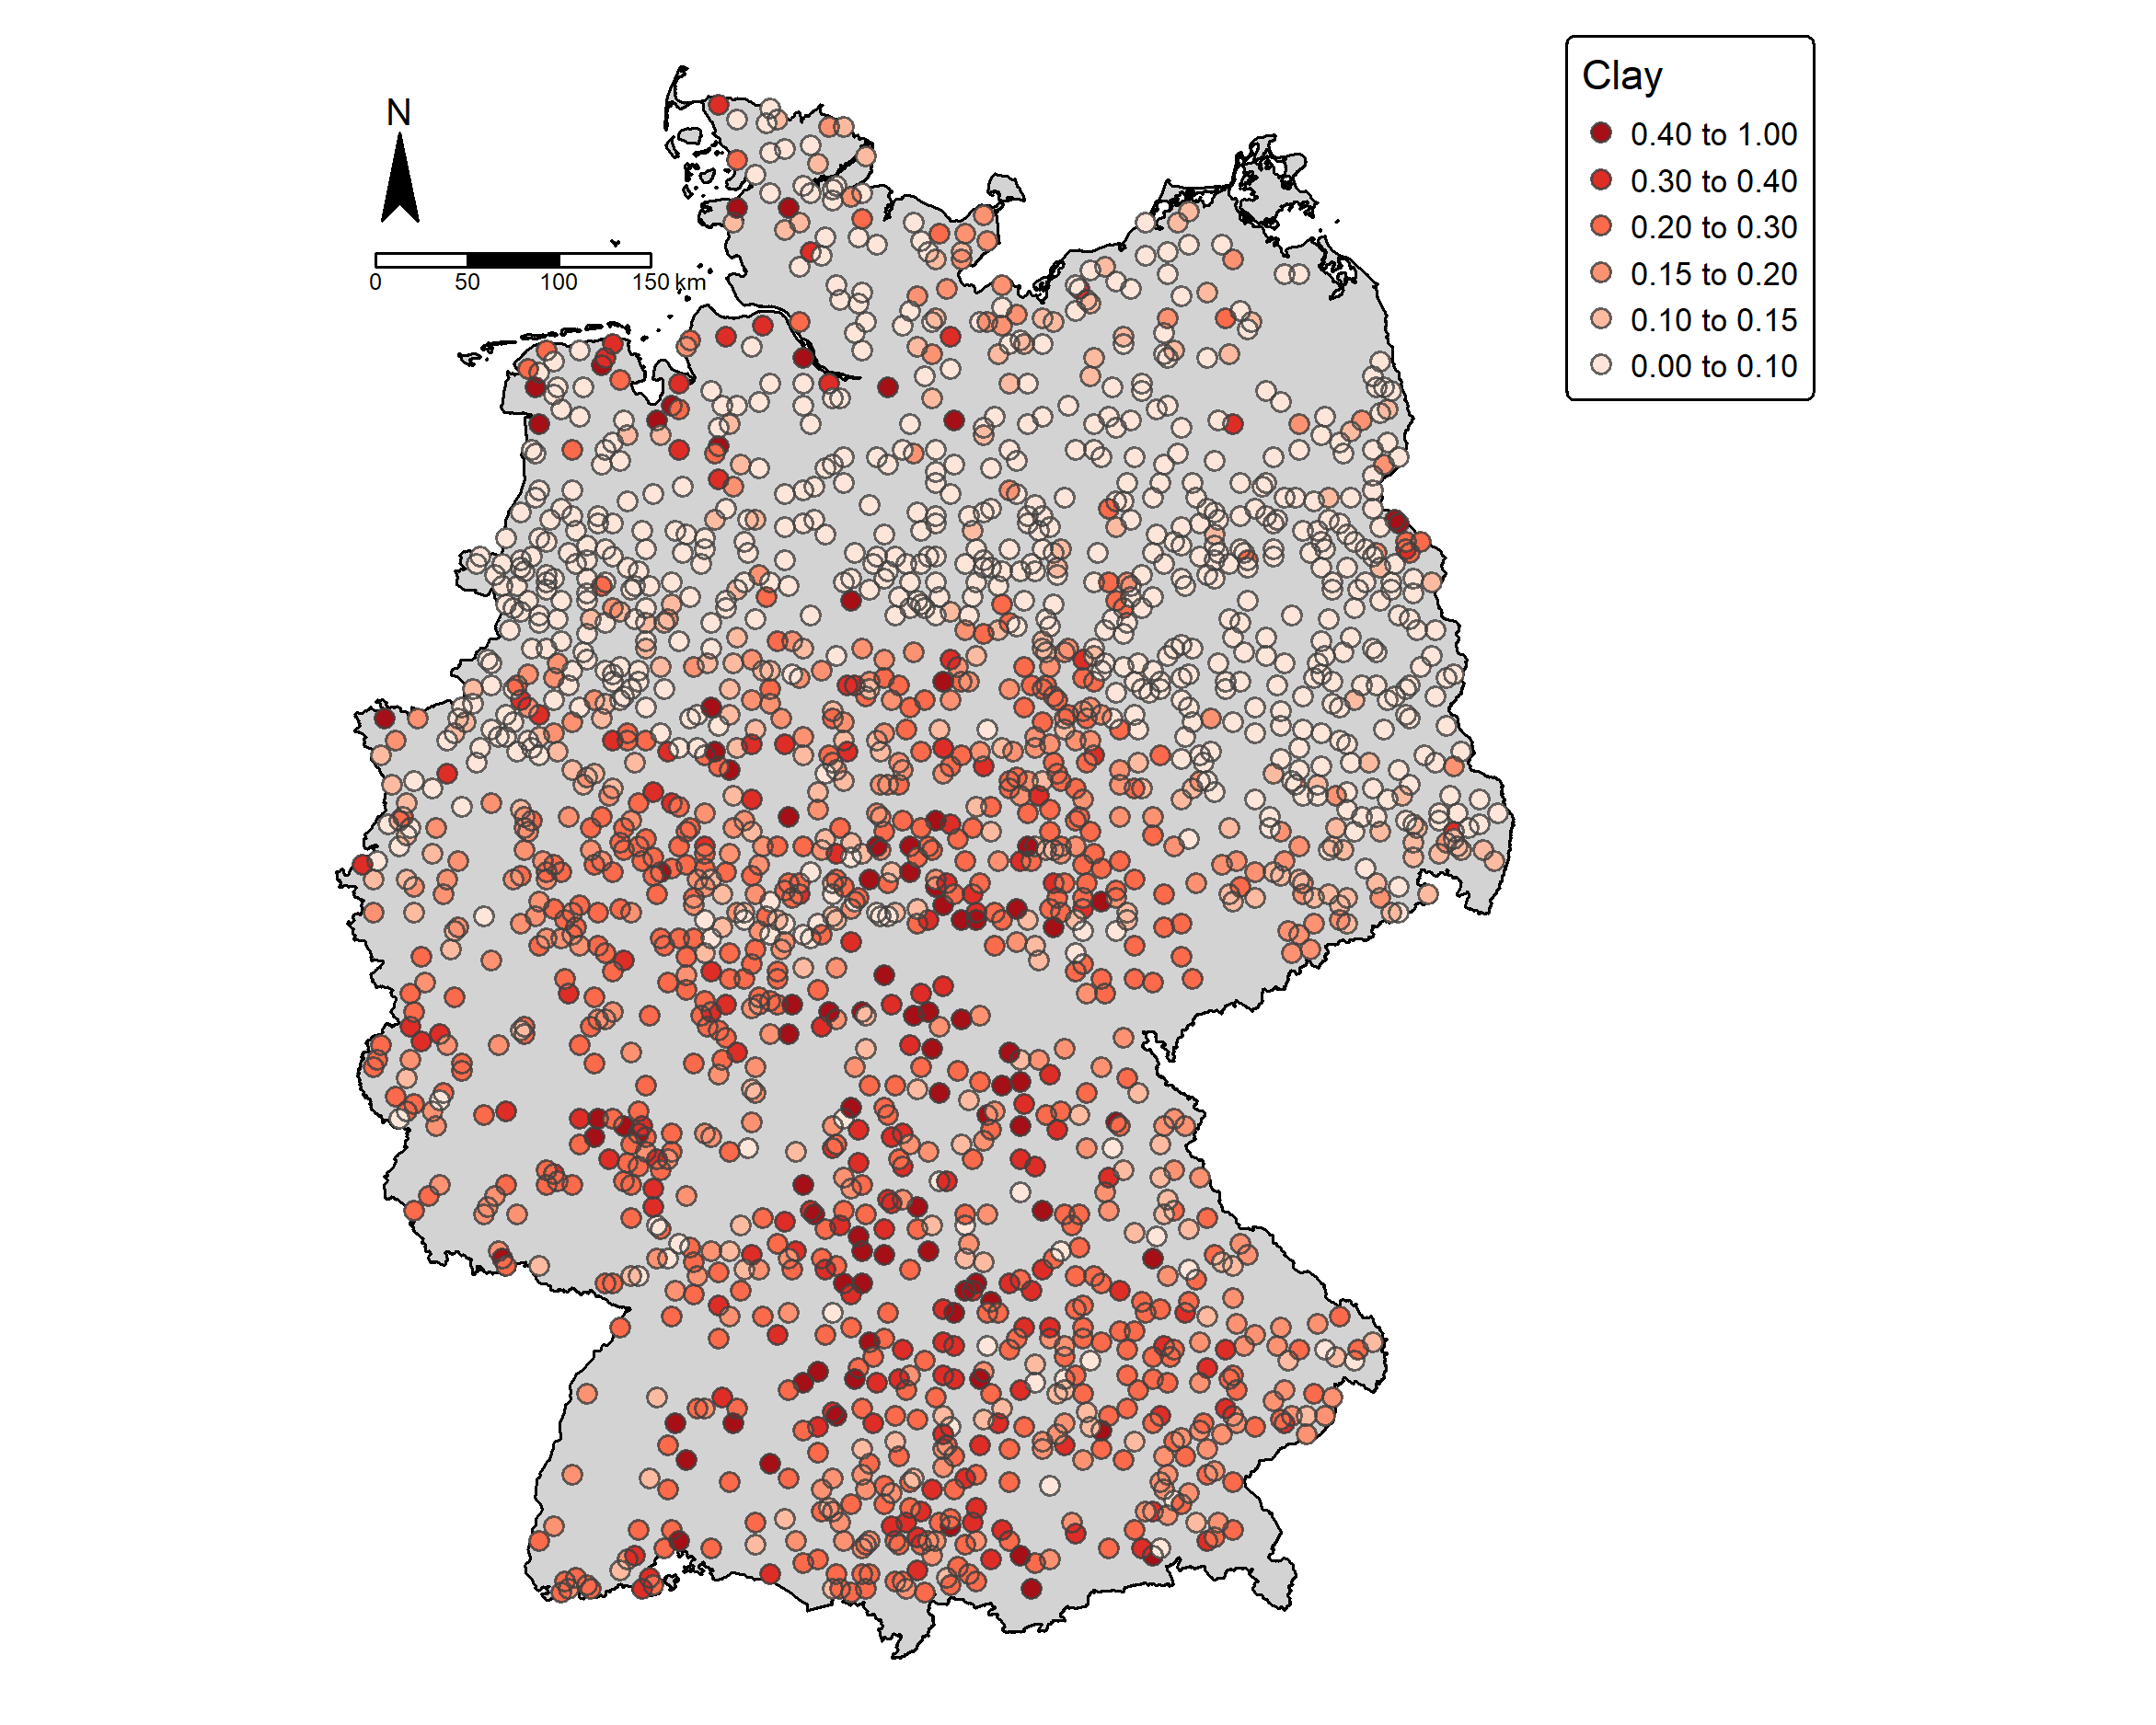
\includegraphics[width=\linewidth]{Figures/pointmap_clay.png}
%             \\ (a) Clay
%         \end{column}
%         \begin{column}{0.33\textwidth}
%             \centering
%             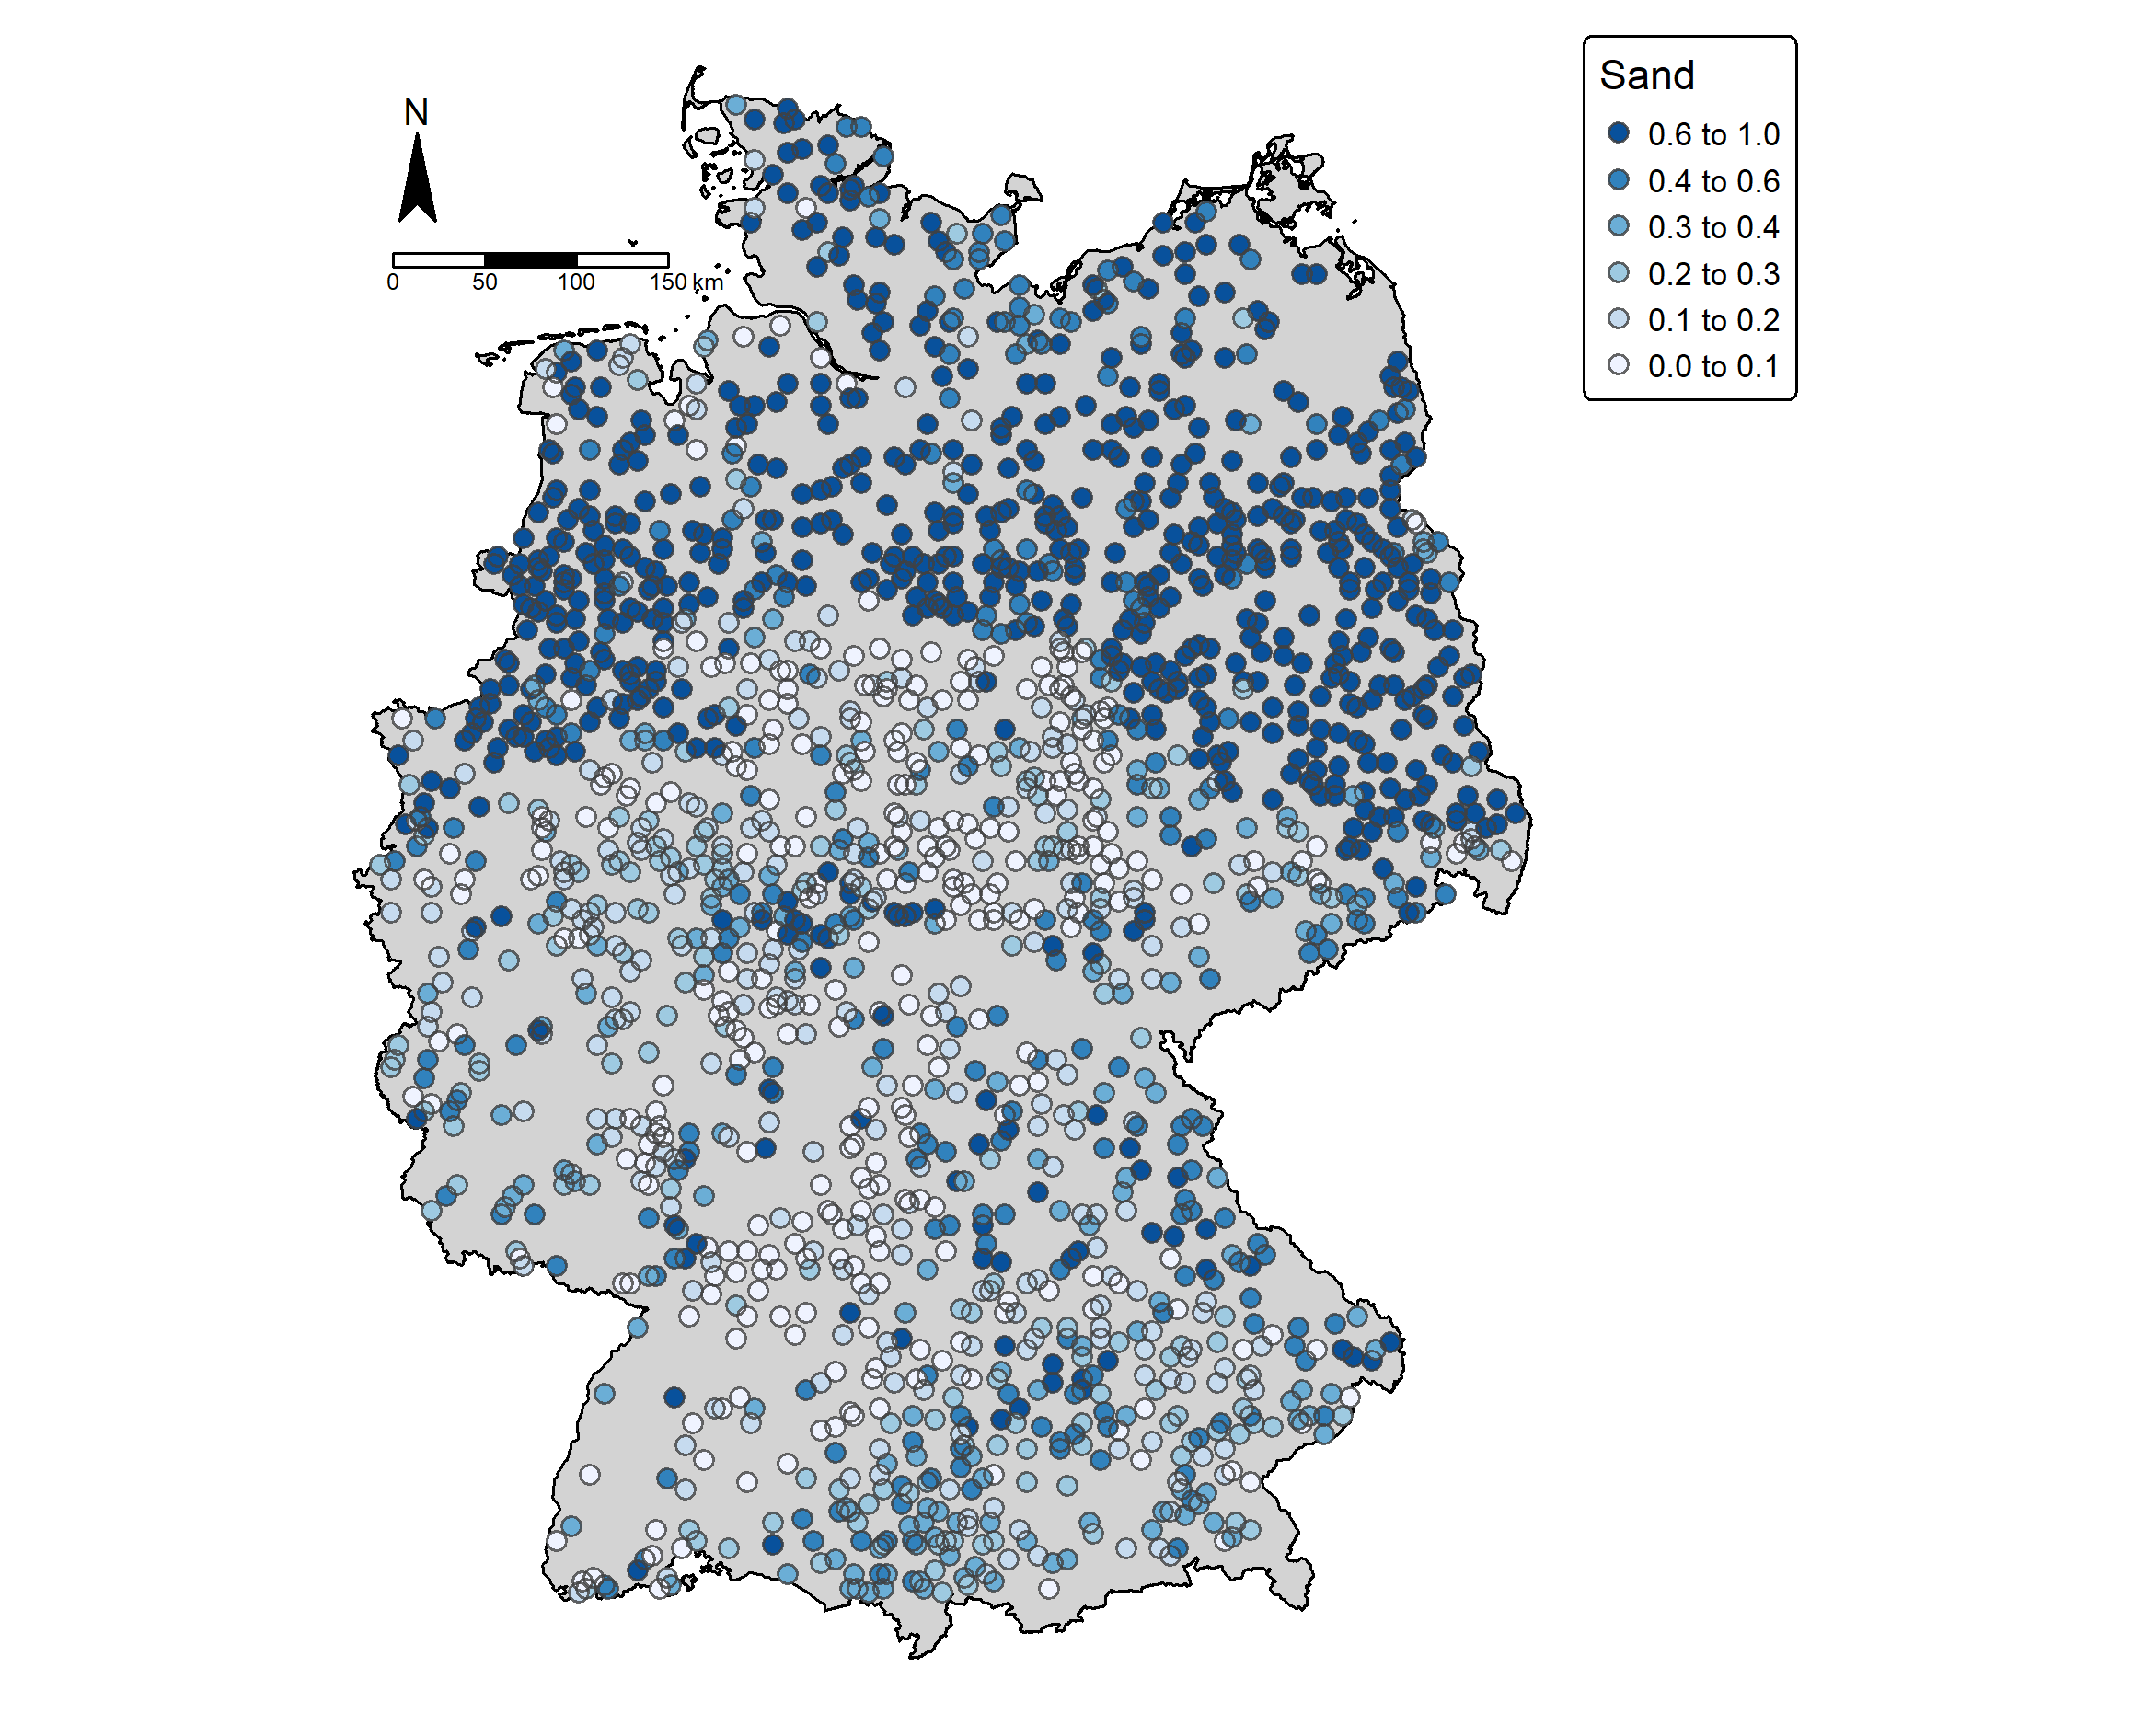
\includegraphics[width=\linewidth]{Figures/pointmap_sand.png}
%             \\ (b) Sand
%         \end{column}
%         \begin{column}{0.33\textwidth}
%             \centering
%             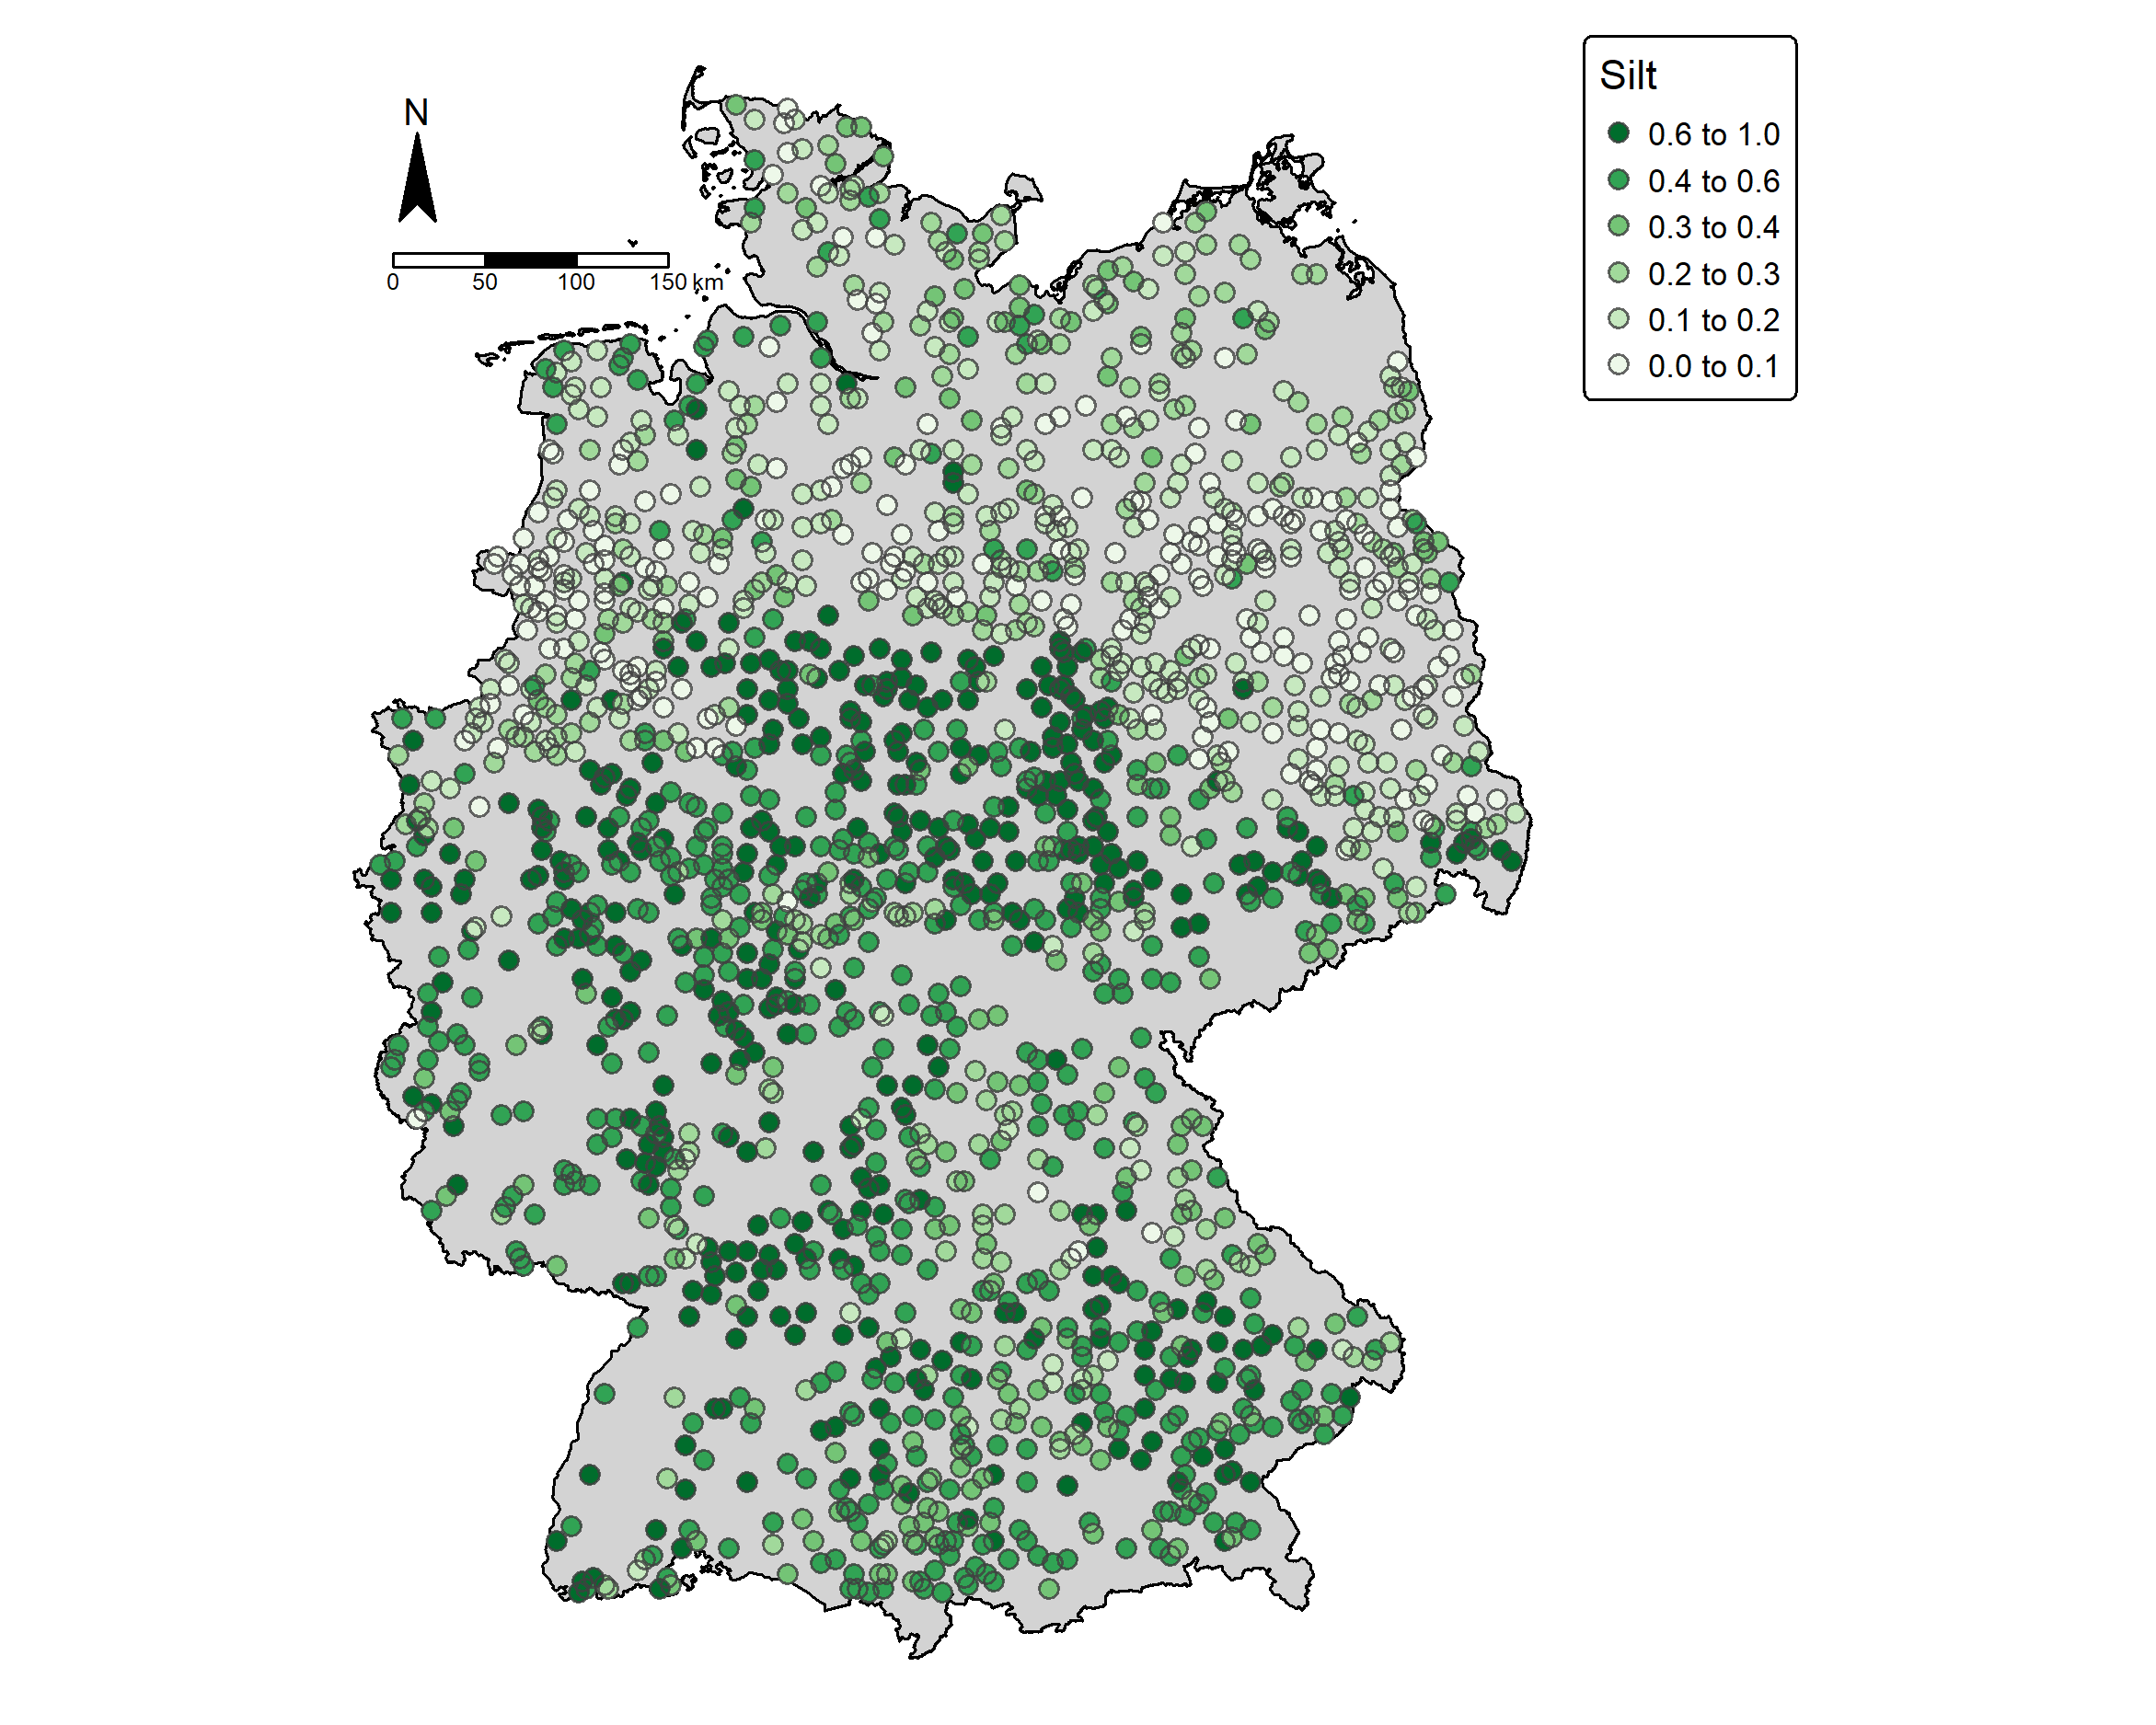
\includegraphics[width=\linewidth]{Figures/pointmap_silt.png}
%             \\ (c) Silt
%         \end{column}
%     \end{columns}
%     \caption{LUCAS soil texture observation locations in Germany: (a) Clay, (b) Sand, (c) Silt (shown as proportions).}
% \end{figure}

% \end{frame}

%% ─── SLIDE 2: Spatial Patterns ─────────────────────────────────────────────
\begin{frame}{Spatial Distribution of Soil Texture}

\begin{columns}

    \begin{column}{0.45\textwidth}
        \begin{itemize}
            \item[1.] Each point represents one \textbf{observation location} in Germany.
            
            \item[2.] The \textbf{colour} of each point indicates the value of the component: darker colours indicate \textbf{higher values}, lighter colours indicate \textbf{lower values}.
            
            \item[3.] \textbf{Clay:} higher values concentrated in the \textbf{south and centre}.
            
            \item[5.] \textbf{Sand:} higher values mostly in the \textbf{north and north-east}.
            
            \item[6.] \textbf{Silt:} more mixed pattern, with elevated values across the \textbf{central belt}.
        \end{itemize}
    \end{column}

    \begin{column}{0.55\textwidth}
        \only<1>{
        \begin{figure}
            \centering
            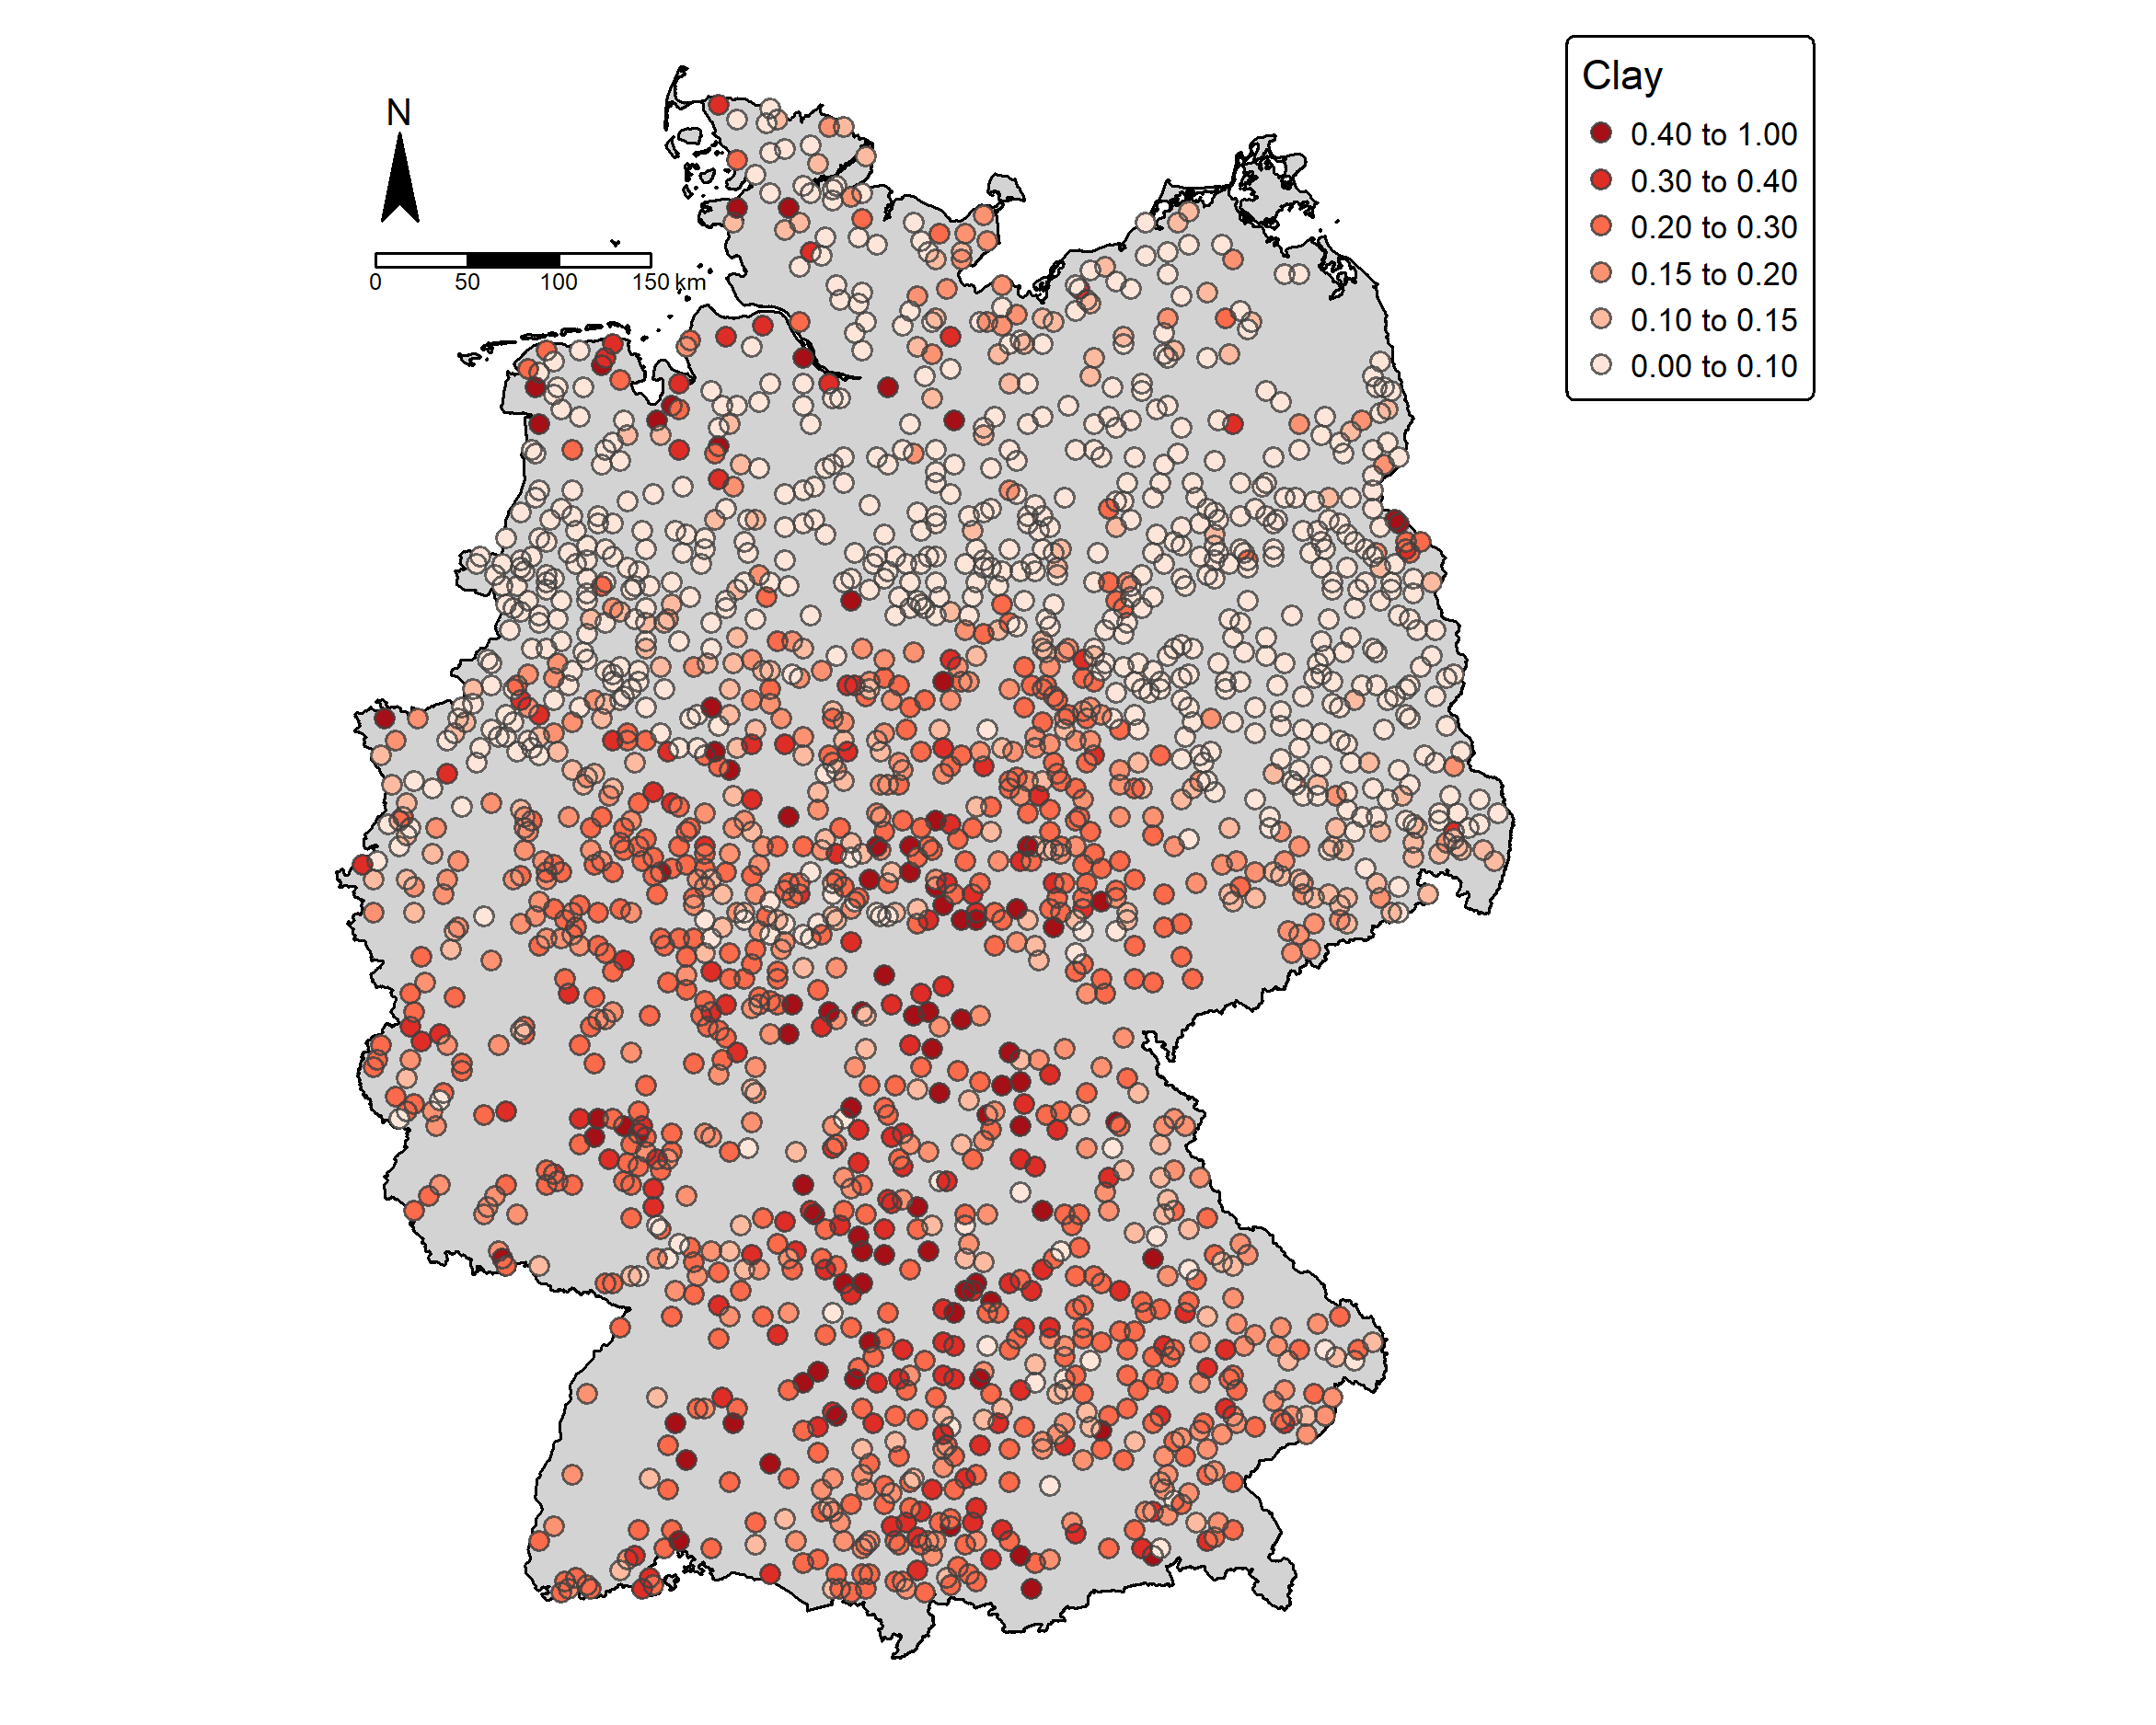
\includegraphics[width=\linewidth]{Figures/pointmap_clay.png}
            \caption{LUCAS soil texture observation locations in Germany: Clay.}
        \end{figure}}
        \only<2>{
        \begin{figure}
            \centering
            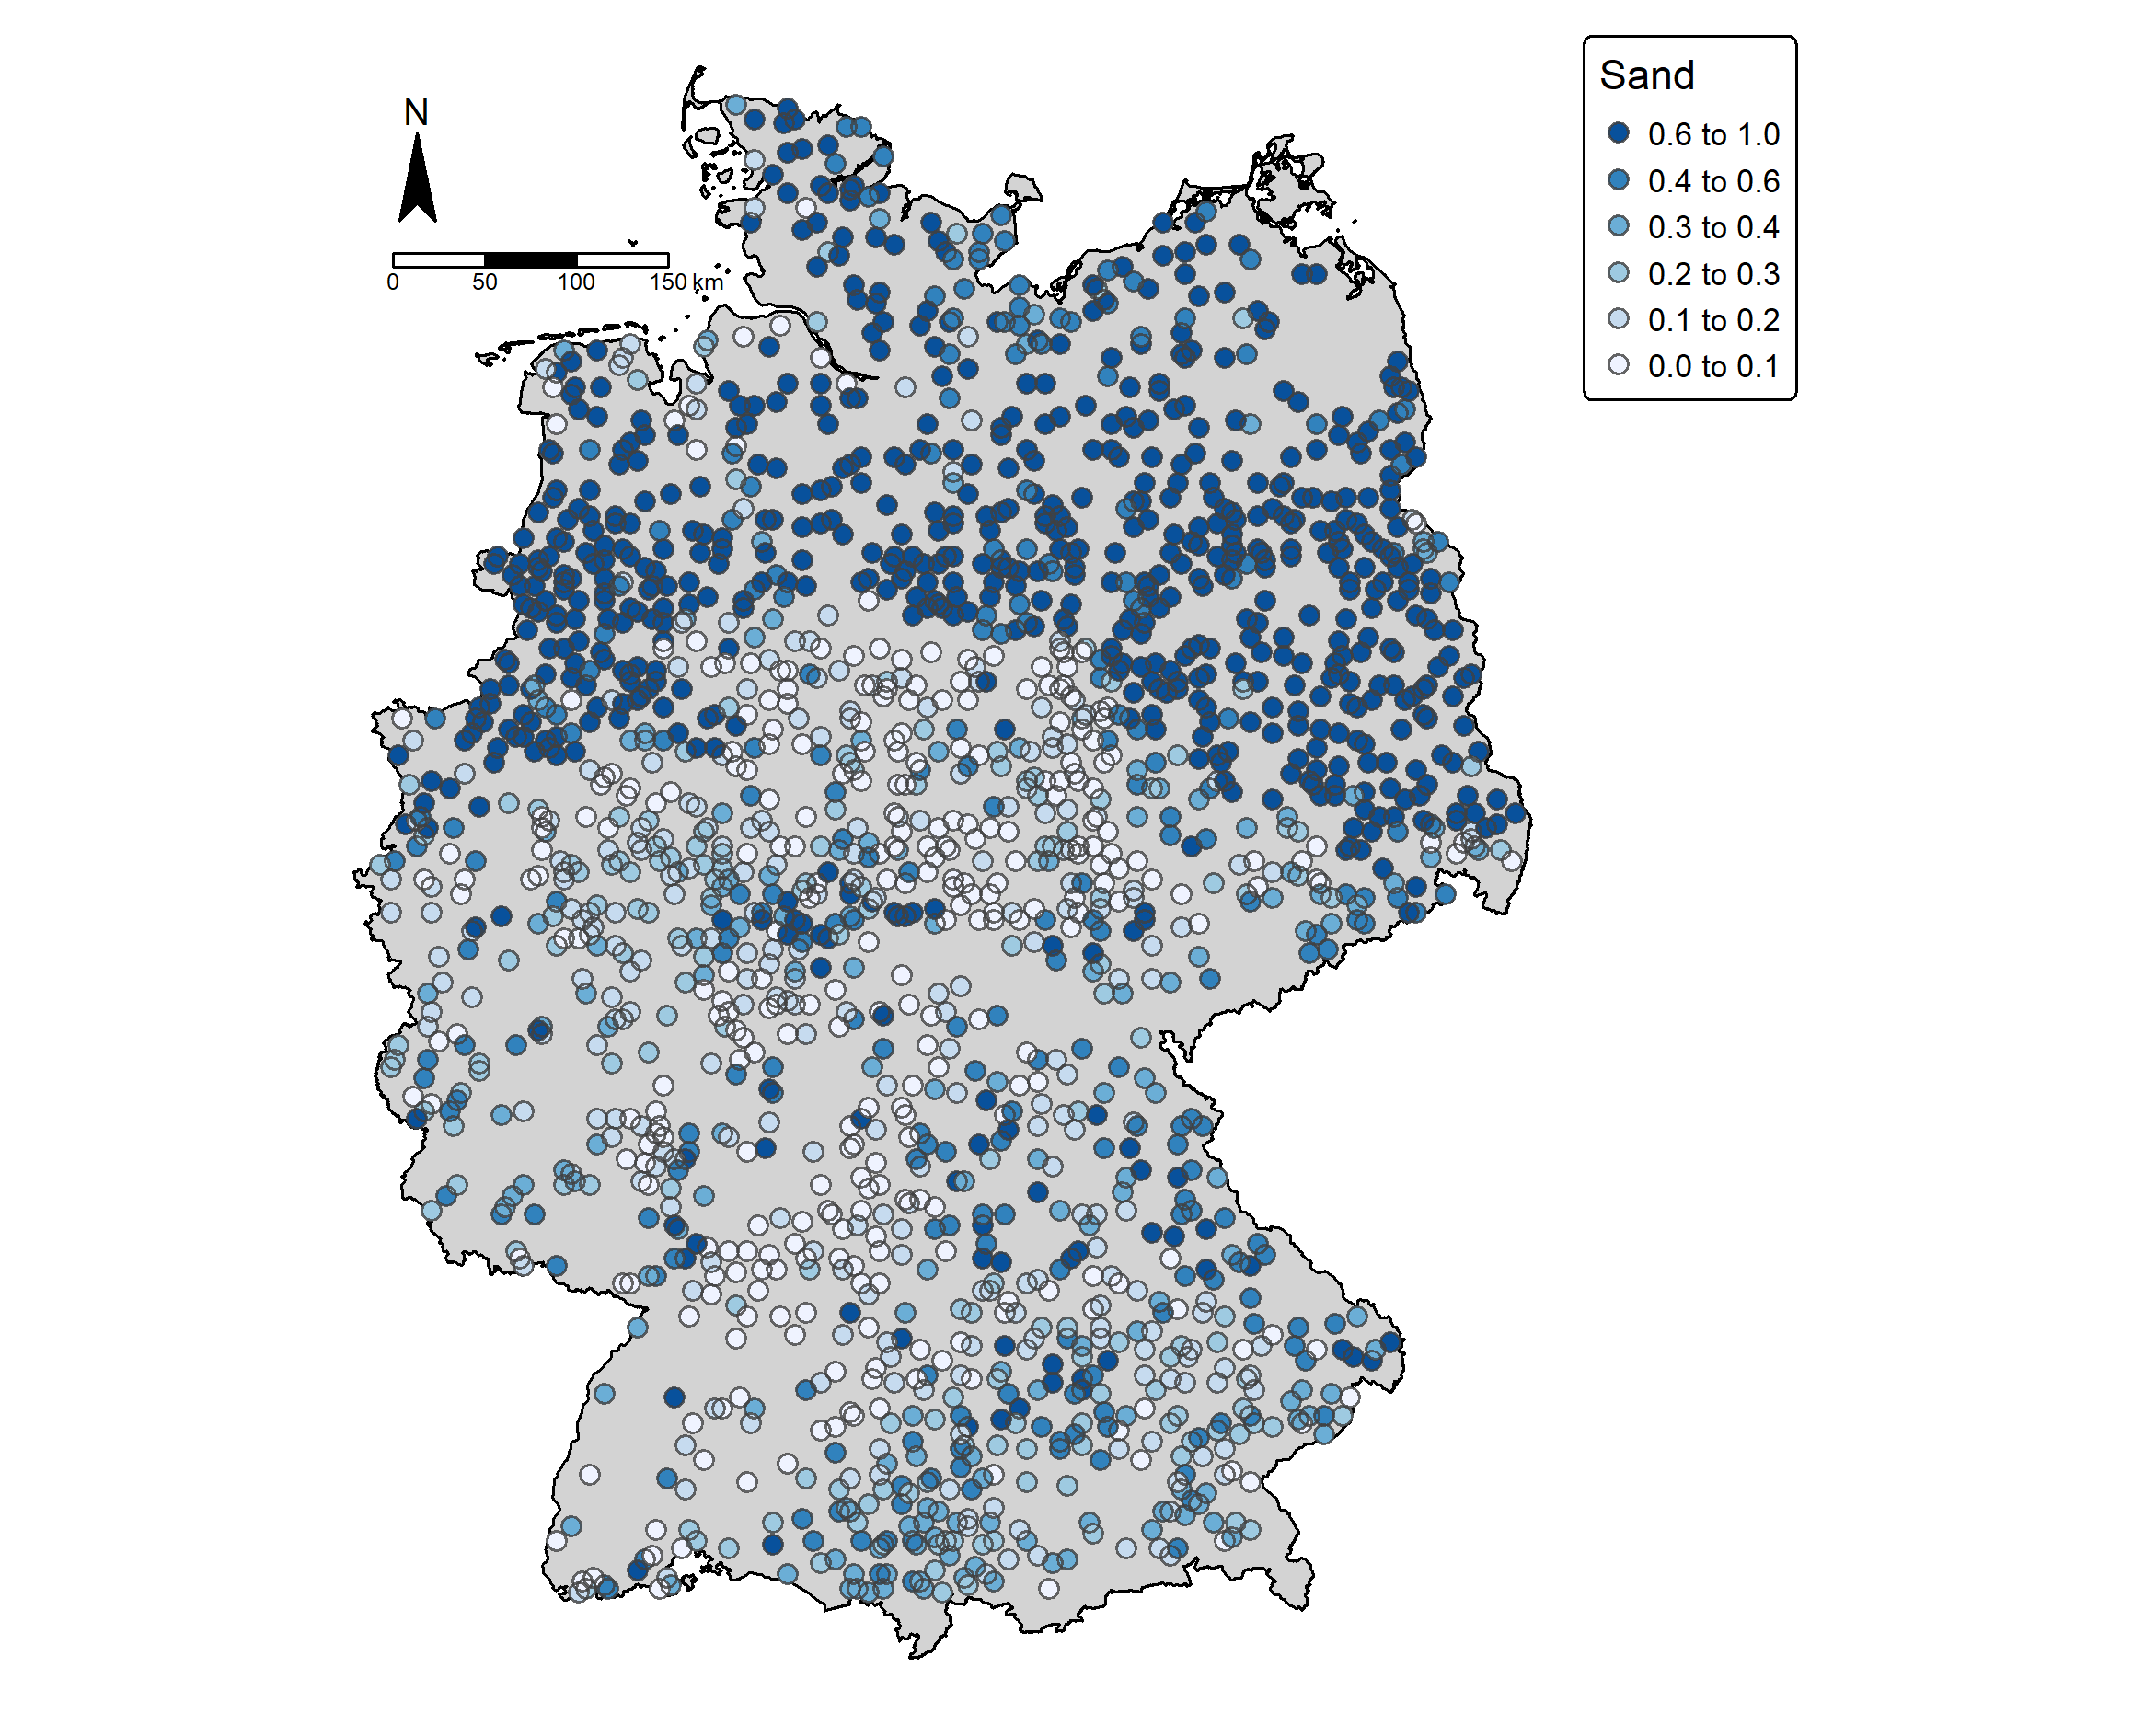
\includegraphics[width=\linewidth]{Figures/pointmap_sand.png}
            \caption{LUCAS soil texture observation locations in Germany: Sand.}
        \end{figure}}
        \only<3>{
        \begin{figure}
            \centering
            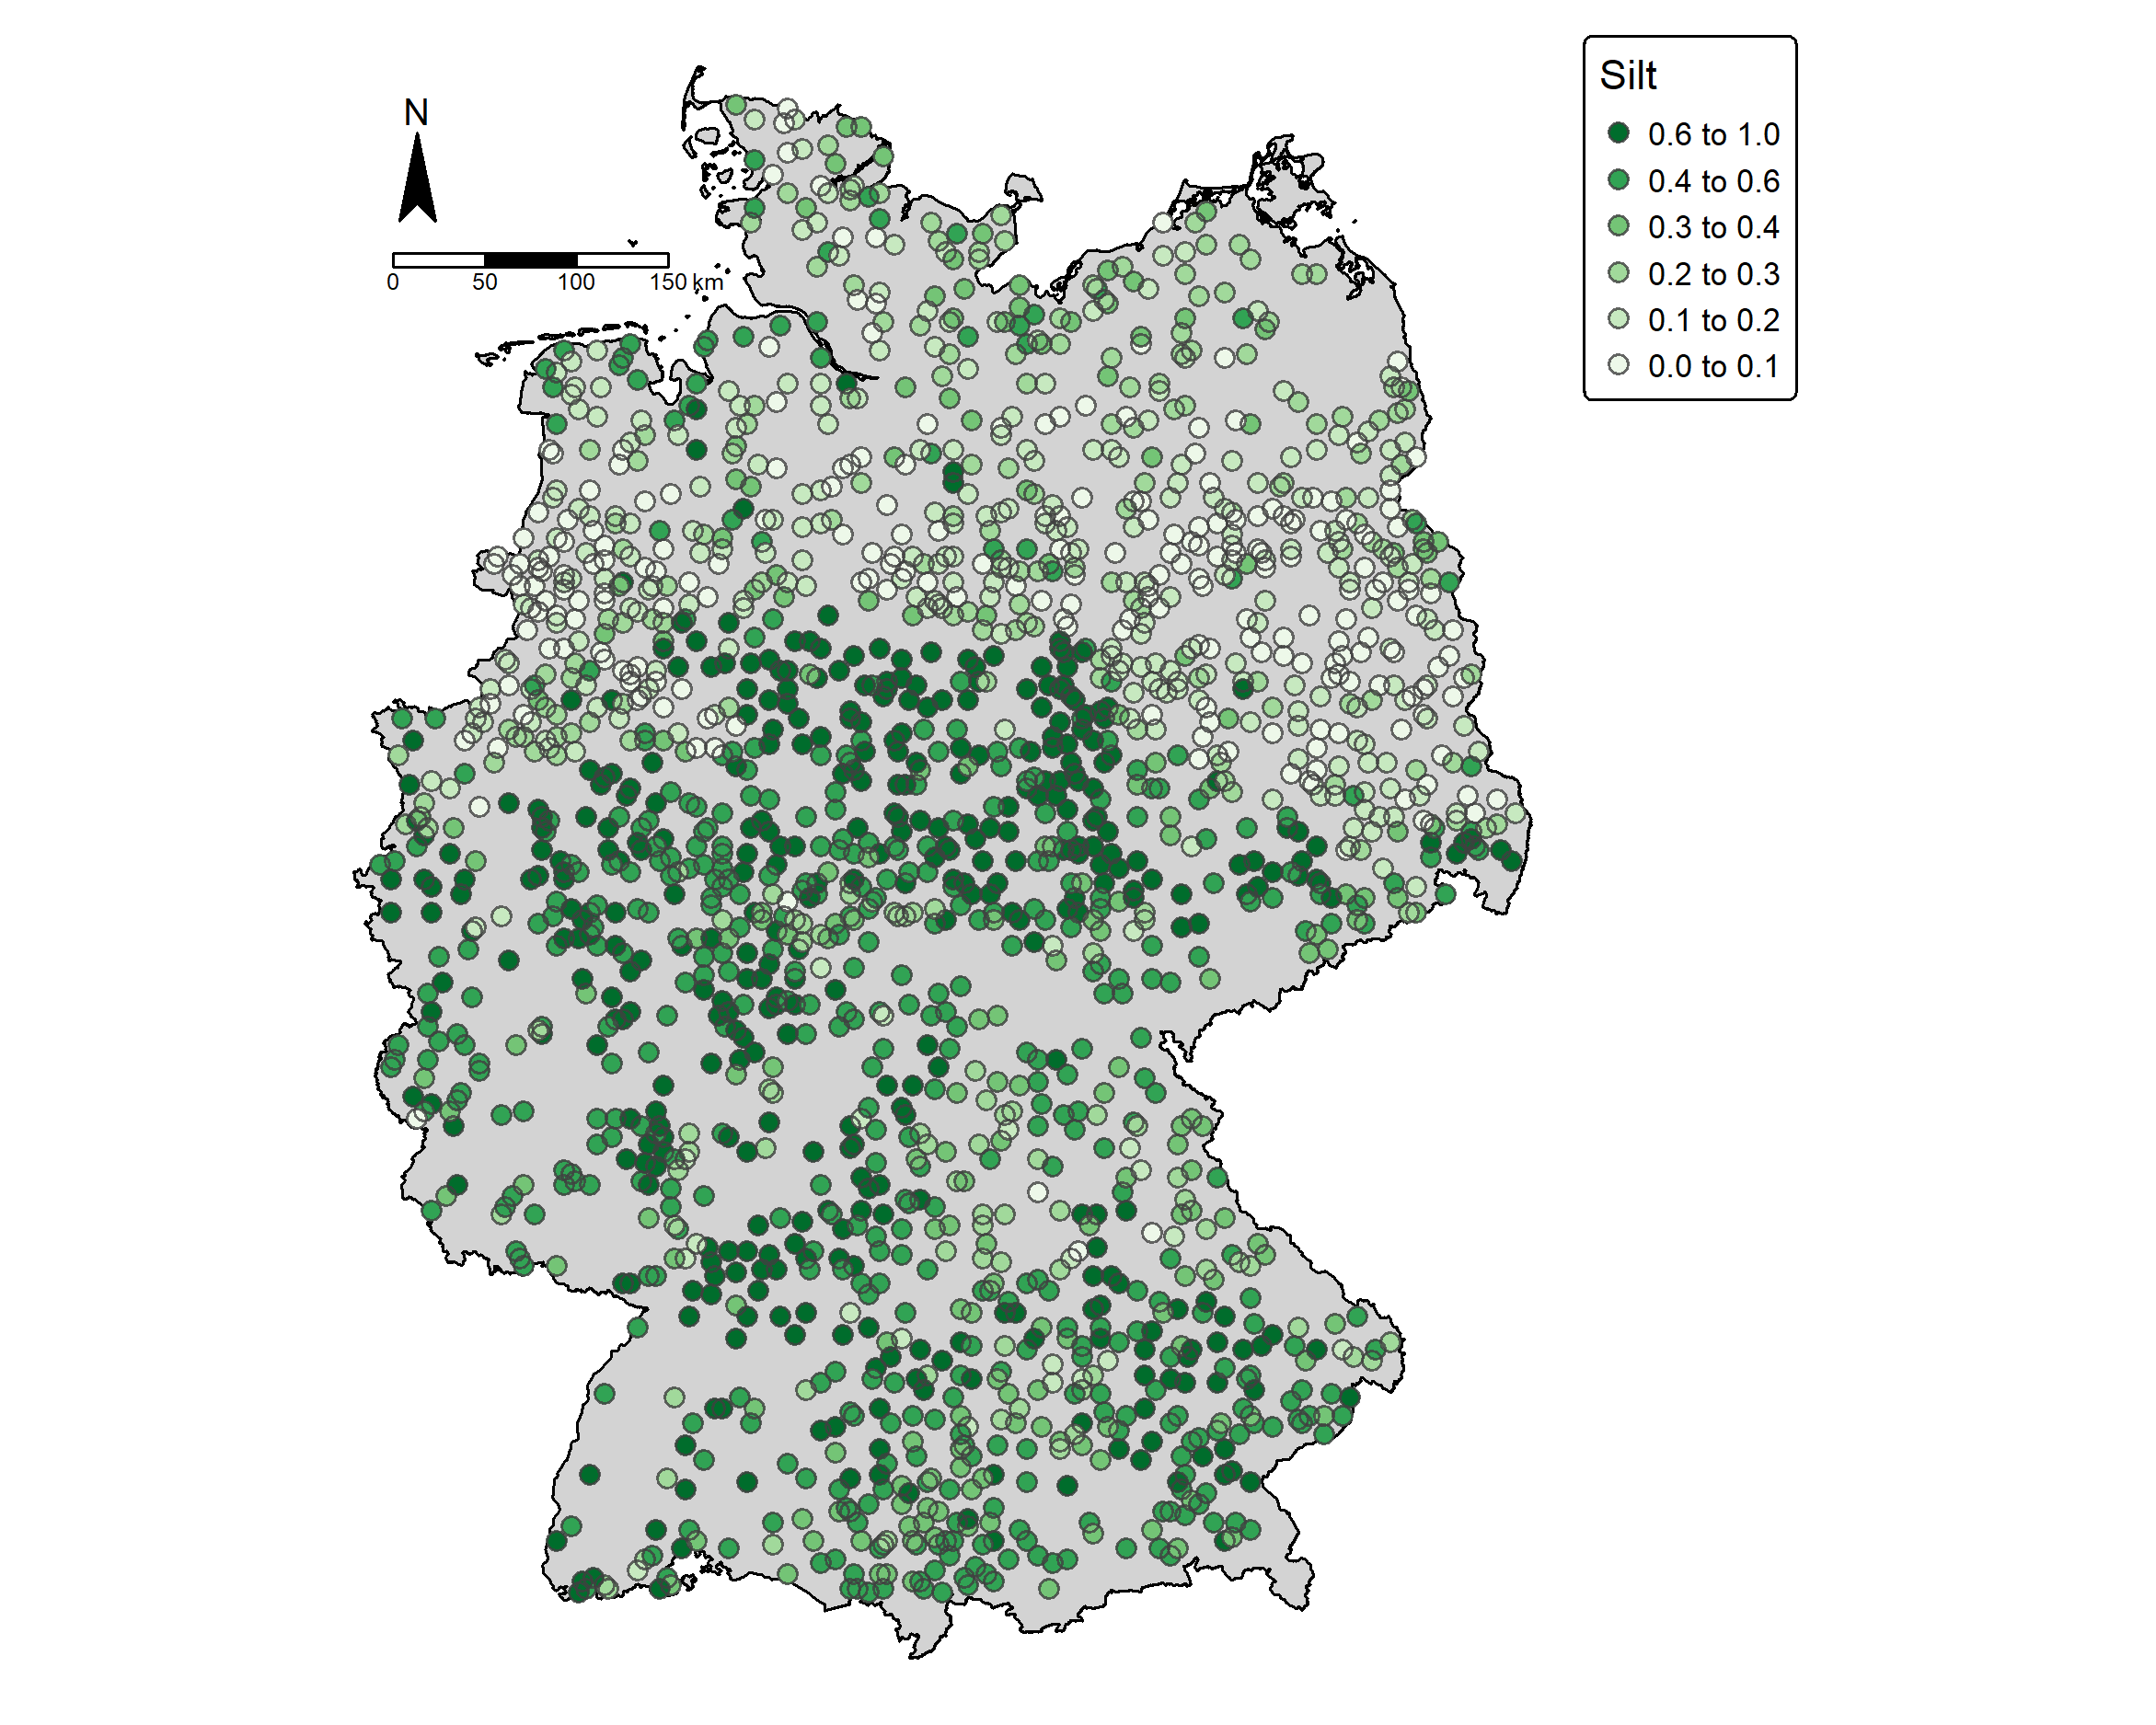
\includegraphics[width=\linewidth]{Figures/pointmap_silt.png}
            \caption{LUCAS soil texture observation locations in Germany: Silt.}
        \end{figure}}
    \end{column}

\end{columns}

\end{frame}

\begin{frame}{Ternary Plot of Soil Texture}

\begin{columns}

    \begin{column}{0.45\textwidth}
        \begin{itemize}
            \item[1.] A \textbf{ternary plot} is a triangle where each corner represents $100\%$ of one component: clay, sand, or silt.

           
            
            \item[2.] Points closer to a corner have a \textbf{higher proportion} of that component.

            \item[3.] Most observations cluster along the \textbf{sand--silt} edge, meaning few samples have high clay content.

            \item[4.] The spread of points reflects the \textbf{large variability} of sand and silt compared to clay.
        \end{itemize}
    \end{column}

    \begin{column}{0.55\textwidth}
        \begin{figure}
            \centering
            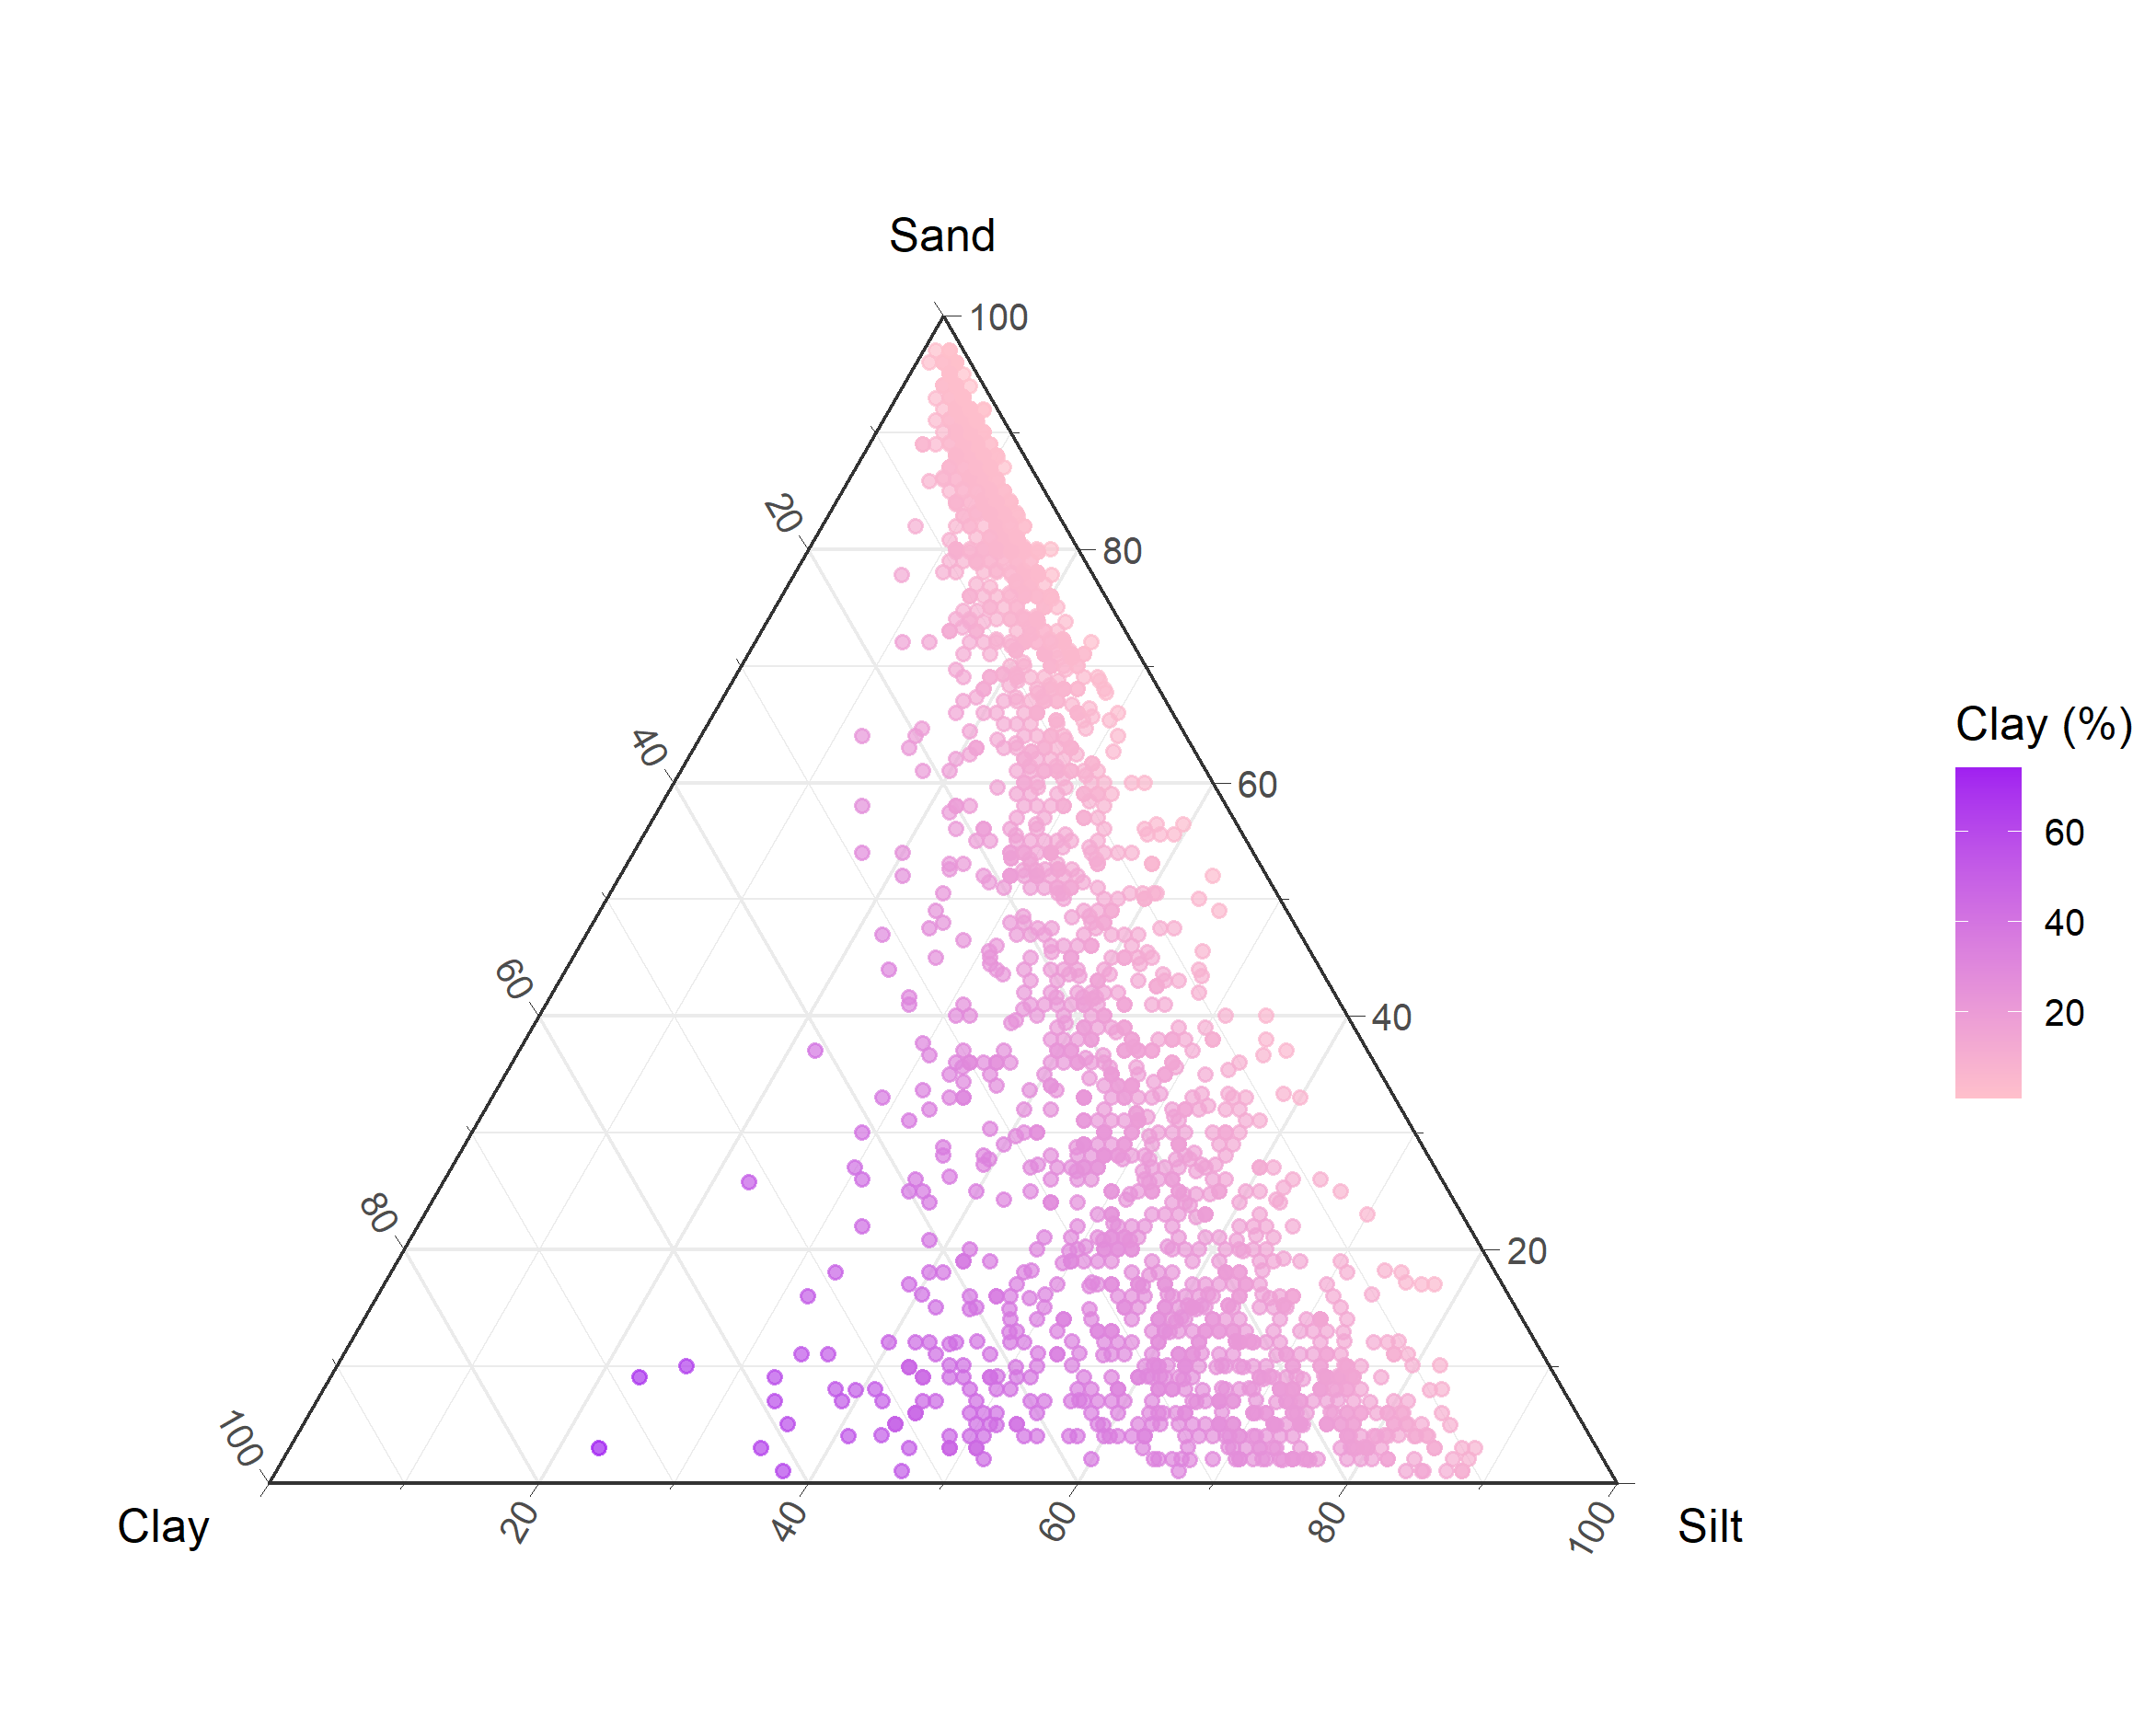
\includegraphics[width=\linewidth]{Figures/point_tern.png}
            \caption{Ternary plot of clay, sand, and silt distributions.}
        \end{figure}
    \end{column}

\end{columns}

\end{frame}

%% ─── SLIDE 4: Modelling Strategies ─────────────────────────────────────────
\begin{frame}{Modelling Strategies}

Five modelling approaches were compared:

\begin{table}
\centering
\small
\begin{tabular}{lccc}
\toprule
Model & Joint estimation & Respects geometry & Transformation \\
\midrule
RF (raw)         & No  & No  & No  \\
MRF (raw)        & Yes & No  & No  \\
ilr-RF           & No  & Yes & Yes \\
ilr-MRF          & Yes & Yes & Yes \\
\textbf{DirichletRF}   & Yes & Yes & No  \\
\bottomrule
\end{tabular}
\caption{Summary of modelling strategies.}
\end{table}

\begin{itemize}
    \item RF and MRF on raw components serve as \textbf{baseline} approaches.
    \item \textbf{DirichletRF} works directly on the simplex without requiring any log-ratio transformation.
\end{itemize}

\end{frame}




%% ─── SLIDE 4: Modelling Strategies ─────────────────────────────────────────
\begin{frame}{Evaluation Metrics}

To compare these models, we used  the Aitchison Distance and the Root Mean Square Error, or RMSE.
\vspace{0.2cm}
\textbf{1. Aitchison Distance:}
\[
AC = \frac{1}{n} \sum_{i=1}^n \sqrt{\sum_{j=1}^k \left(\log\frac{Y_{ij}}{g(\mathbf{Y}_i)} - \log\frac{\hat{Y}_{ij}}{g(\hat{\mathbf{Y}}_i)}\right)^2},
\]
\[
\text{where} \quad g(\mathbf{Y}_i) = \left(\prod_{j=1}^k Y_{ij}\right)^{1/k}
\]
\textit{Measures compositional dissimilarity using log-ratio geometry.}

\vspace{0.3cm}
\textbf{2. Root Mean Square Error (RMSE):}
$
\text{RMSE}_k =  \sqrt{\frac{1}{n} \sum_{i=1}^n (Y_{ij} - \hat{Y}_{ij})^2}
$

\vspace{0.3cm}
\textbf{Interpretation:} Lower values for both metrics indicate better predictive accuracy.
\end{frame}



\begin{frame}{Parameter Tuning and Cross-Validation}

\begin{itemize}
    \item[1.] All models were assessed using \textbf{10-fold nested cross-validation},
    with the same folds shared across methods to ensure a fair comparison.

    \item[2.]  Each random forest model was fitted with \textbf{500 trees}.

    \item[3.]  Hyper-parameters were selected by grid search:
    \begin{itemize}
        \item[3.1]  minimum node size: $\{2, 5, 10\}$
        \item[3.2] $m_{\mathrm{try}}$: $\{23, 29, 35, 41, 47, 53, 59, 65\}$
    \end{itemize}

    \item[4.] For \textbf{DirichletRF}, minimum node size was fixed at 5 for computational efficiency.

    \item[5.] Performance was quantified using \textbf{RMSE} and \textbf{Aitchison distance}.

    \item[6.] For the  comparison, models were refitted on the full dataset using
    the best hyper-parameters from the inner folds.
\end{itemize}

\end{frame}




%% ─── SLIDE 6: Results ───────────────────────────────────────────────────────
\begin{frame}{Results: RMSE and Aitchison Distance}

\begin{table}
\centering
\small
\caption{RMSE and Aitchison Distance (AC) across modelling approaches.}
\begin{tabular}{lccccc}
\toprule
 & RF & ilr-RF & MRF & ilr-MRF & \textbf{DirichletRF} \\
\midrule
\multicolumn{6}{c}{\textbf{RMSE}} \\
\midrule
Clay        & 0.086 & 0.086 & 0.088 & 0.087 & \textbf{0.085} \\
Sand        & 0.186 & 0.181 & 0.188 & 0.182 & \textbf{0.168} \\
Silt        & 0.148 & 0.145 & 0.150 & 0.146 & \textbf{0.135} \\
Aggregated  & 0.140 & 0.137 & 0.142 & 0.138 & \textbf{0.130} \\
\midrule
\multicolumn{6}{c}{\textbf{Aitchison Distance (AC)}} \\
\midrule
AC & 0.852 & 0.788 & 0.861 & 0.798 & \textbf{0.766} \\
\bottomrule
\end{tabular}
\end{table}

\begin{itemize}
    \item \textbf{DirichletRF} achieves the lowest RMSE across all components and the smallest AC.
    \item The largest gains are observed for \textbf{sand} and \textbf{silt}.
    \item ilr-based models only marginally outperform their untransformed counterparts.
\end{itemize}

\end{frame}


%% ─── FRAME 1: Cross-Validation Explanation ──────────────────────────────────
\begin{frame}{Publication}

\begin{center}
\vfill

\begin{block}{}
\begin{center}
\textbf{Dirichlet Random Forest for Predicting Compositional Data}\\[0.4em]
\end{center}
\end{block}

\vspace{0.5em}

\textbf{Authors:}\\[0.3em]
\underline{Masoumifard, K.}, van der Westhuizen, S., Gardner-Lubbe, S.

\vspace{0.8em}

\textbf{In:}\\[0.3em]
A. Bekker et al.\ (Eds.),\\
\textit{Environmental Modelling with Contemporary Statistics:\\
Learning, Directionality, and Space-Time Dynamics}\\[0.3em]
CRC Press\\[0.3em]
ISBN: 9781032903910

\vfill
\end{center}

\end{frame}
% %\begin{frame}{Library on GitHub}
\only<1>{
\note{
For our DDRF method, we have developed an R library. It is available on CRAN and on GitHub. You can access it using this QR code.

}

  \begin{center}

    \qrcode{https://github.com/Xaleed/DirichletRF.git}
 \end{center}
    
    \centering
    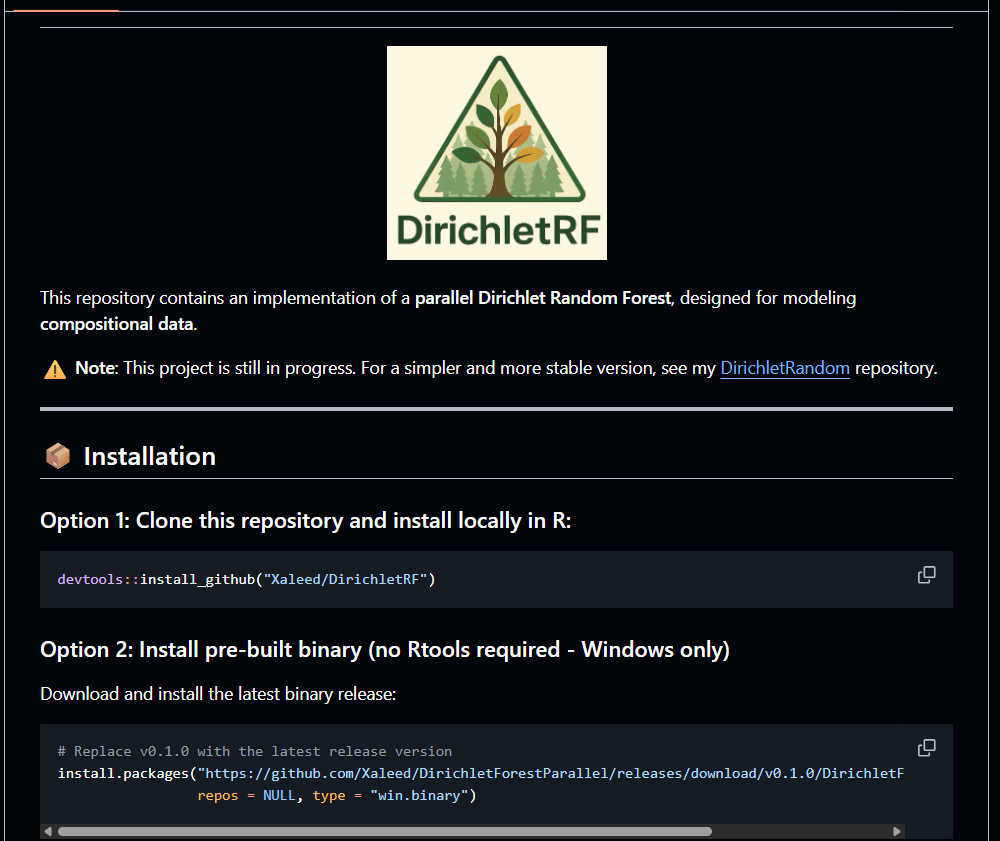
\includegraphics[width=0.45\linewidth]{slides/github.png}
    \caption{}
}
% \only<2>{
% \note{
% We developed an R library for this Random Forest model. This library implements the Random Forest in parallel and provides both predictions and empirical distributions. The parameters can be estimated using either Maximum Likelihood Estimation (MLE) or the Method of Moments (MoM), with MoM being the default option.

% }
%   \begin{center}

%     \qrcode{https://github.com/Xaleed/DirichletRF.git}
%  \end{center}
% %\vspace{0.3cm}

% \textbf{Key Features:}
% \begin{itemize}
% \item[\textcolor{blue}{\large$\blacktriangleright$}] Dirichlet distribution-based splits (likelihood maximization)
% \item[\textcolor{blue}{\large$\blacktriangleright$}] Parallel processing (Unix/Mac fork, Windows cluster)
% \item[\textcolor{blue}{\large$\blacktriangleright$}] Two purpose: Prediction vs. Distributional
% \item[\textcolor{blue}{\large$\blacktriangleright$}] Two parameter estimation methods (MoM, MLE)
% \end{itemize}


% }
    
\only<2>{
% \note{
% Most of the parameters are the same as in other well-known libraries. Here, we introduce two new parameters: \texttt{method} and \texttt{store\_samples}. I will briefly explain both.


% }
\begin{table}
\small
\begin{tabular}{lp{3cm}p{6cm}}
\toprule
\textbf{Parameter} & \textbf{Default} & \textbf{Description} \\
\midrule
\texttt{num.trees}  & 100          & Number of trees in the forest \\
\texttt{max.depth}  & 10           & Maximum tree depth \\
\texttt{min.node.size} & 5         & Minimum observations per leaf node \\
\texttt{mtry}       & $\sqrt{p}$   & Candidate features at each split \\
\texttt{seed}       & 123          & Random seed for the C++ RNG \\
\texttt{\textcolor{blue}{est.method}} & \texttt{"mom"} & Dirichlet estimation: \texttt{"mom"} or \texttt{"mle"} \\
\texttt{num.cores}  & $-1$         & OpenMP threads ($-1$ = all cores minus one) \\
\bottomrule
\end{tabular}
\end{table}
}
\end{frame}




% \begin{frame}{Conclusion}
%     \begin{itemize}

%     \item[\textcolor{blue}{\large$\blacktriangleright$}] 
%     \textbf{For compositional data}, we adapt Random Forest splitting rules to respect the geometry of the simplex, avoiding the limitations and potential bias introduced by traditional transformations to real space.
%     \vspace{1.1em}

%     \item[\textcolor{blue}{\large$\blacktriangleright$}] 
%     \textbf{Based on  comparison results, the model shows strong and stable performance}
%     across a wide range of scenarios.
%     \vspace{1.1em}

%     \item[\textcolor{blue}{\large$\blacktriangleright$}] 
%     \textbf{We also provide an open-source implementation} 
%     available as a Git/R package.
% \end{itemize}
% \end{frame}



% %
\begin{frame}
 
\frametitle{\resizebox{.95\linewidth}{!}{%
Addressing Dirichlet's Limitations: Extensions \& Alternatives}}
\note{Now, I want to talk about three useful versions of the Dirichlet distribution:

First, the Zero-Inflated Dirichlet. This model is good when we have many zeros in the data. The standard Dirichlet cannot handle zeros well, but this one can.

Second, the Nested Dirichlet. The standard Dirichlet assumes all parts are negatively related. This is not always true in real data. The nested version helps fix that.

Third, the Kummer–Dirichlet. This model is better when the data has outliers. It is more flexible and gives more stable results.}
\begin{itemize}
  \item[\textcolor{blue}{\large$\blacktriangleright$}] \textbf{ Zero-Inflated Dirichlet Models:}  
  Handle compositional data with many zeros.

  \item[\textcolor{blue}{\large$\blacktriangleright$}] \textbf{ Nested–Dirichlet Models:}  
  Address the limitation of standard Dirichlet where all components are negatively correlated.

  \item[\textcolor{blue}{\large$\blacktriangleright$}] \textbf{Kummer–Dirichlet Models:}  
  Offer greater robustness to outliers compared to the standard Dirichlet.
\end{itemize}


\end{frame}

\begin{frame}
\frametitle{Distributional Dirichlet Random Forests (DRF)}
\note{
Another idea that I really like is to fit an empirical probability function.

Actually, we can fit a probability function on the training dataset. Then, for a new observation, we can evaluate this probability function to obtain its predicted distribution.

Actually, we can fit a probability function on the training dataset. This method was introduced in 2022. I will not go into the details of how it works. I have a simple example to explain it, but I will skip it to save time.
}

\begin{equation*}
P(Y = y_i \mid X = \mathbf{x}_{\text{new}}) = w_i(\mathbf{x}_{\text{new}}), \quad i = 1, \dots, n, \quad \sum_{i=1}^{n} w_i(\mathbf{x}_{\text{new}}) = 1.
\end{equation*}

\vspace{0.5em}
\begin{block}{}
The formula for the normalized weight $w_i$ is:
\[
w_i(\mathbf{x}_{\text{new}})
= \frac{1}{B} \sum_{k=1}^B 
\frac{\mathbf{1}\!\left(\mathbf{x}_{\text{new}} \in L_k(i)\right)}{|L_k(i)|}.
\]
where $|L_k(i)|$ is the size of the terminal node in tree $k$ where $\mathbf{x}_{\text{new}}$ falls.
\end{block}
\end{frame}



\begin{frame}[plain]
  \begin{center}
    \vspace{2cm}

    {\Huge \textbf{Thank You!}\par}

    \vspace{1cm}

    
\includegraphics[width=0.15\linewidth]{slides/DirichletRF.jpg}

    %\vspace{0.8cm}

    % QR code (requires: \usepackage{qrcode})
    \qrcode[height=1.8cm]{https://github.com/Xaleed/DirichletRF.git}

    \vspace{0.1cm}

    {\small QR code for the GitHub repository}

  \end{center}
\end{frame}


% %


\begin{frame}{Why Ambiguous!}
   \only<1>{

   \frametitle{Principles of CODA}
      \begin{itemize}
       \item 
   \textbf{scale invariance},
   \item
   \textbf{permutation invariance}, and 
   \item \textbf{subcompositional coherence}
   If \( \Delta_p(\mathbf{x}, \mathbf{y}) \) denotes a distance measure between compositions with \( p \) parts, then
    \begin{equation*}
    \Delta_k(\mathbf{x}, \mathbf{y}) \geq \Delta_d(\mathbf{x}_d, \mathbf{y}_d),
    \end{equation*}
    where \( \mathbf{x}, \mathbf{y} \) are compositions with \( k \) parts, and \( \mathbf{x}_d, \mathbf{y}_d \) are corresponding subcompositions with \( d < k \) parts.
    \end{itemize}}
\only<2>{
\textbf{\textcolor{blue}{Question 1:}} Are these principles designed to achieve consistent results with the original data $\mathbf{Y}$?  

The arguments supporting $\mathbf{a}(\mathbf{Y})$ are rarely evaluated for consistency with the original vector $\mathbf{Y}$, even though Aitchison himself criticized standard statistical approaches for inconsistency with the original data.
}

\only<3>{
As an illustration, consider
\[
\mathbf{S}(\mathbf{Y}) = \Big( \frac{Y_1}{Y_1 + Y_2}, \frac{Y_2}{Y_1 + Y_2} \Big) = (U, 1-U).
\]
\textbf{\textcolor{blue}{Can we assume that \(U\) follows a Beta distribution?}}

\textbf{\textcolor{red}{Aitchison's critique:}} For \(U\) to follow a Beta distribution,
\[
Y_i \sim^{\text{iid}} \text{Gamma}(\alpha_i, \lambda), \quad i=1,2.
\]
This generalizes naturally to the Dirichlet distribution.

His proposal instead:
\[
\left(\frac{1}{2}\ln\frac{Y_1}{Y_2}, \frac{1}{2}\ln\frac{Y_2}{Y_1}\right)
\]
}

\only<4>{
\textbf{\textcolor{blue}{Question 2:}} Are these principles designed to provide non-spurious correlations?

Correlations among components of $\mathbf{a}(\mathbf{Y})$ are themselves spurious.
}

\only<5>{
\textbf{Spurious correlation example:}

Even if  
\[
\operatorname{corr}(Y_1, Y_2)=0,
\]
we usually observe
\[
\boxed{
\operatorname{corr}\Big(\frac{Y_1}{S}, \frac{Y_2}{S}\Big) \neq 0, \quad S=\sum_{j=1}^{D} Y_j
}
\]
\textbf{Reason:} shared denominator induces dependency.
}

\only<6>{
\[
\boxed{
\operatorname{corr}\Big(\frac{Y_1}{S}, \frac{Y_2}{S}\Big)
=
\frac{
\mathbb{E}\Big(\frac{Y_1 Y_2}{S^2}\Big) - \mathbb{E}\Big(\frac{Y_1}{S}\Big)\mathbb{E}\Big(\frac{Y_2}{S}\Big)
}{
\sqrt{\operatorname{Var}\Big(\frac{Y_1}{S}\Big)} \sqrt{\operatorname{Var}\Big(\frac{Y_2}{S}\Big)}
}
}
\]

\textbf{Key point:} The formula is mathematically valid; the issue is interpretation:
\[
\operatorname{corr}\Big(\frac{Y_1}{S}, \frac{Y_2}{S}\Big) \not\Rightarrow \operatorname{corr}(Y_1,Y_2)
\]
}

\only<7>{
\textbf{Frequently emphasized in CODA:}

\begin{block}{Different denominators}
\[
\left(\frac{Y_1}{S_4},\frac{Y_2}{S_4},\frac{Y_3}{S_4},\frac{Y_4}{S_4}\right),\quad
\left(\frac{Y_1}{S_3},\frac{Y_2}{S_3},\frac{Y_3}{S_3}\right)
\]
\end{block}

\begin{alertblock}{Claimed problem}
\[
\operatorname{corr}\Big(\frac{Y_1}{S_4}, \frac{Y_2}{S_4}\Big) \neq \operatorname{corr}\Big(\frac{Y_1}{S_3}, \frac{Y_2}{S_3}\Big)
\]

\textbf{Both correlations are spurious.}  
It is unclear why equality between two spurious correlations should matter.
\end{alertblock}
}

\only<8>{
\begin{block}{ILR (or Other) Transformed Coordinates}

\begin{minipage}{0.48\textwidth}
\centering
\textbf{} \\[2mm]
\scalebox{0.75}{$
\mathbf{T}_4 = T\Big(\frac{Y_1}{S_4},\frac{Y_2}{S_4},\frac{Y_3}{S_4},\frac{Y_4}{S_4}\Big):(T_1,T_2,T_3,T_4)
$} \\[2mm]
\scalebox{0.75}{$
\mathbf{T}_3 = T\Big(\frac{Y_1}{S_4},\frac{Y_2}{S_4},\frac{Y_3}{S_4}\Big):(T_1,T_2,T_3)
$}
\end{minipage}
\hfill
\begin{minipage}{0.48\textwidth}
\centering
\textbf{} \\[2mm]
\scalebox{0.75}{$
\mathbf{T}'_4 = T\Big(\frac{Y'_1}{S'_4},\frac{Y'_2}{S'_4},\frac{Y'_3}{S'_4},\frac{Y'_4}{S'_4}\Big):(T'_1,T'_2,T'_3,T'_4)
$} \\[2mm]
\scalebox{0.75}{$
\mathbf{T}'_3 = T\Big(\frac{Y'_1}{S'_4},\frac{Y'_2}{S'_4},\frac{Y'_3}{S'_4}\Big):(T'_1,T'_2,T'_3)
$}
\end{minipage}

\end{block}


\begin{alertblock}{Subcompositional Coherence}
\scalebox{0.85}{\[
D_3(\mathbf{T}_3,\mathbf{T}'_3) \le D_4(\mathbf{T}_4,\mathbf{T}'_4)
\]}
\begin{center}
\textbf{\large Surprisingly, the correlations between components remain \textcolor{red}{spurious}, 
but we cannot work in the simplex space accordingly.}
\end{center}
\end{alertblock}
}

\only<9>{
\textbf{\textcolor{blue}{Question 2:}} Are these principles designed to provide non-spurious correlations?  The answer is no.
}

\only<10>{
\textbf{\textcolor{blue}{Question 3:}} Are these principles designed to satisfy theoretical requirements?

It is important to note that \(\mathbf{s}(\cdot)\)  is subset of real space and therefore inherit its standard geometric structure, rendering all conventional mathematical operations well-defined.
}

\only<11>{
\textbf{\textcolor{blue}{Question 4:}} Are these principles widely accepted?  The answer is no.
}

\end{frame}



\begin{frame}{Critics of CoDA: Early and Ongoing}
A number of authors have questioned the strict log-ratio framework
promoted by the “CoDa School.” Major groups include:
\scriptsize   % shrinks everything but remains readable


\begin{itemize}\itemsep1pt
    \item \textbf{Watson}: objections to distance measures and geometry
    \item \textbf{Zier \& Rehder}: challenges to mathematical definitions
    \item \textbf{Butler \& Glasbey}: alternative approaches for zeros
    \item \textbf{Stewart \& Field}: practical issues in real applications
    \item \textbf{Tsagris et al.}: limits for highly variable data
    \item \textbf{Scealy \& Welsh}: critique of the Principles themselves
\end{itemize}



\end{frame}




\begin{frame}{Key Critics: D.F. Watson}
\scriptsize   % shrinks everything but remains readable

    \begin{itemize}
        \item \textbf{D.F. Watson} was a central figure in early debates against Aitchison's log-ratio methods.
        \item **Main Criticism Focus:**
        \begin{itemize}
            \item Questioned the fundamental need for "scale invariance," a core principle of the CoDa School.
            \item His exchanges with Aitchison in \textit{Mathematical Geology} (1989-1992) were instrumental in the development of the CoDa Principles, though from a critical stance.
            \item The text notes that "Watson \& Philip (1989) ... did not see the need for scale invariance."
        \end{itemize}
        \item Tragically, his contributions were cut short due to a contentious exchange where Aitchison used derogatory language.
    \end{itemize}
\end{frame}
\begin{frame}{Key Critics: Zier \& Rehder}
\scriptsize   % shrinks everything but remains readable

    \begin{itemize}
        \item \textbf{Zier \& Rehder} (1998, 2001) continued to raise points against the CoDa School's established views.
        \item **Main Criticism Focus:**
        \begin{itemize}
            \item Challenged technical issues, particularly related to the mathematical definition of a metric within compositional data analysis.
            \item Like Watson, they "did not see the need for scale invariance," arguing it problematic if compositions are strictly defined as summing to one.
            \item Their arguments highlighted that even Aitchison's own earlier work might not have strictly adhered to the current CoDa definition of compositions and scale invariance.
        \end{itemize}
        \item Despite making "some good points," their criticisms were "dismissed relatively easily" by the CoDa School, partly due to perceived technical mistakes on their part.
    \end{itemize}
\end{frame}
\begin{frame}{Key Critics: Butler \& Glasbey}
\scriptsize   % shrinks everything but remains readable

    \begin{itemize}
        \item \textbf{Butler \& Glasbey} (2008) represent a more recent wave of critics whose methods were deemed "unapproved" by the CoDa School.
        \item **Main Criticism Focus:**
        \begin{itemize}
            \item Developed "otherwise sensible analysis" methods that did not conform to the CoDa Principles.
            \item Were compelled to "list and explain their 'failings' relative to the Principles."
            \item Their work highlighted that theoretical difficulties with the Principles meant their methods could only be used as "diagnostic tool or for exploratory analysis" according to CoDa proponents.
            \item This illustrates how the Principles act as a barrier to new methodological developments.
        \end{itemize}
    \end{itemize}
\end{frame}
\begin{frame}{Key Critics: Stewart \& Field, Tsagris et al., Scealy \& Welsh}
\scriptsize   % shrinks everything but remains readable

    \begin{itemize}
        \item \textbf{Stewart \& Field (2010), Tsagris, Preston \& Wood (2011), and Scealy \& Welsh (2011a, 2011b)} also demonstrate the practical limitations of the CoDa School's exclusive approach.
        \item **Main Criticism Focus:**
        \begin{itemize}
            \item Provided "interesting real examples where important practical differences produced by a variety of methods are highlighted."
            \item Showed that the differences between various methods become particularly important for \textbf{highly variable data near or on the boundary of the simplex}.
            \item \textbf{Scealy & Welsh (2011a, 2014, the source text)} specifically critique the **motivation, justification, and relevance of the Principles themselves**, particularly subcompositional coherence.
            \item They argue against the logical basis for scale invariance and subcompositional dominance, proposing alternatives like "amalgamations" as more suitable 'marginals'.
        \end{itemize}
    \end{itemize}
\end{frame}
\begin{frame}{Conclusion on Criticisms}
\scriptsize   % shrinks everything but remains readable

    \begin{itemize}
        \item These critics collectively highlight significant issues:
        \begin{itemize}
            \item The contested definition of a "composition."
            \item The rigid and sometimes illogical foundations of the CoDa Principles (e.g., scale invariance, subcompositional coherence).
            \item The active dismissal of valid alternative methods simply for not conforming to these Principles.
            \item The practical limitations of the CoDa approach, especially with challenging data.
        \end{itemize}
        \item The text emphasizes that the existence and application of these Principles in such a restrictive way is "unusual, perhaps even unique, in statistical data analysis."
    \end{itemize}
\end{frame}



\begin{frame}{The Aitchison-Watson Debate: A Contentious Beginning}
\scriptsize   % shrinks everything but remains readable

    \begin{itemize}
        \item The foundational "Principles of Compositional Data Analysis" largely evolved from a series of intense exchanges.
        \item Primarily, this involved papers and letters between \textbf{J. Aitchison} (as the defender/proponent of log-ratio methods) and \textbf{D.F. Watson} (as a critic of the nascent CoDa School's approach).
        \item These debates, published in \textit{Mathematical Geology} from 1989-1992, set the stage for much of the field's development and controversies.
        \item However, the intellectual exchange took a negative turn:
        \begin{itemize}
            \item Aitchison is noted to have used the word "stupid" in reference to Watson's arguments.
            \item This pejorative remark led to \textbf{Watson discontinuing his contributions} to the debate, effectively silencing a critical voice.
        \end{itemize}
        \item This event highlights how personal attacks can impede scientific discourse and shape the trajectory of a research field.
        \item Scealy & Welsh (2014) emphasize that "the exchange between Watson and Aitchison had a negative impact on both sides and contributed directly to the situation in modelling and analysing compositional data that we have today."
    \end{itemize}
\end{frame}


% %\begin{frame}{Simplex space}
\only<1>{
\note{
In this presentation, I will frequently refer to simplex space. 
A simplex space is collection of vectors with non-negative values that always sum to a constant.
This space is known as the \emph{simplex} and it is common to set \( k = 1 \).
We refer to data from this space as \emph{compositional data}.
}

\vspace{1em}

A simplex is a convex space of all vectors with non-negative components that sum to a constant. 

\begin{center}
\colorbox{blue!10}{\parbox{0.8\textwidth}{
\begin{center}
\[
S^c_k = \left\{ (y_1, \dots, y_k)^\top \in \mathbb{R}^k \,\middle|\, y_i \geq 0, \ \sum_{i=1}^k y_i = \textcolor{blue}{c} \right\}
\]
\end{center}
}}
\end{center}

It is common to set \(  \textcolor{blue}{c = 1} \). We refer to data from this space as \emph{compositional data}.
}

\only<2>{
\note{Another important space in the context of compositional data is the Aitchison space. This space is a log-transformed version of the simplex. Another important log-ratio transformation is the isometric log-ratio (ILR) transformation.
In reality, there is a wide variety of log-ratio transformations of the simplex space. }
Aitchison space:
\begin{center}
\colorbox{blue!10}{\parbox{1\textwidth}{
\begin{center}
\[
A_k = \left\{\left(\ln\!\left(\frac{Y_1}{g(\mathbf{Y})}\right), \ldots, \ln\!\left(\frac{Y_{k}}{g(\mathbf{Y})}\right)\right); g(\mathbf{Y}) = \left(\prod_{i=1}^{k} Y_i\right)^{1/{k}}\right\}
\]
\end{center}
}}
\end{center}
}
\end{frame}


\begin{frame}{Compositional data}
\only<1>{
\note{
Consider a vector with \(K\) components, where the only constraint is that all components are non-negative. Two important transformations of this vector are the following vectors. 

1. transform data to simplex space

2. transform data to Aitchison space

so we have original vector, simplex vector and Aitchison vector.

In general, the original vector \(\mathbf{Y} = (Y_1, \ldots, Y_K) \in \mathbb{R}_+^K\) cannot be recovered from these transformations, because they remove information about the absolute scale of the components. However, the simplex representation and the Aitchison representation can be recovered from one another.

There are some challenges in interpreting results that are based on the Simplex or Aitchison space.
}

Consider a vector \(\mathbf{Y} = (Y_1, Y_2, \ldots, Y_k) \in \mathbb{R}_+^k\). Two commonly used transformations of \(\mathbf{Y}\) are of particular interest:  

\begin{equation*}
\mathbf{S}_{k}(\mathbf{Y}) = \left(\frac{Y_1}{\sum_{i=1}^{k} Y_i}, \ldots, \frac{Y_{k}}{\sum_{i=1}^{k} Y_i}\right),
\end{equation*}

and  

\begin{equation*}
\mathbf{A}_{k}(\mathbf{Y}) = \left(\ln\!\left(\frac{Y_1}{g(\mathbf{Y})}\right), \ldots, \ln\!\left(\frac{Y_{k}}{g(\mathbf{Y})}\right)\right),
\end{equation*}

where \(g(\mathbf{Y}) = \left(\prod_{i=1}^{k} Y_i\right)^{1/{k}}\) denotes the geometric mean of \(\mathbf{Y}\). 
}

\only<2>{
\note{
it is simplest case of these two spaces.
}
Consider a vector \(\mathbf{Y} = (Y_1, Y_2) \in \mathbb{R}_+^2\). 

\begin{equation*}
\mathbf{S}(\mathbf{Y}) = \left(\frac{Y_1}{Y_1+Y_2},  \frac{Y_2}{Y_1+Y_2}\right),
\end{equation*}

and  

\begin{equation*}
\mathbf{A}(\mathbf{Y}) = \left(\frac{1}{2}\ln\!\left(\frac{Y_1}{Y_2}\right), \frac{1}{2}\ln\!\left(\frac{Y_2}{Y_1}\right)\right),
\end{equation*}

where \(g(\mathbf{Y}) = \left(\prod_{i=1}^2 Y_i\right)^{1/2}\) denotes the geometric mean of \(\mathbf{Y}\). 
}

\only<3>{
\note{
One important point is that the correlation between components 1 and 2 is \(-1\) in both the simplex and the Aitchison space, no matter what the correlation between \(Y_1\) and \(Y_2\) is.

this type correlation between components in the simplex or in the Aitchison space should \textbf{not} be interpreted as the correlation between the original components of \(\mathbf{Y}\). 

This is also true for higher dimensions. The correlations in these spaces can be far from zero, even when the true correlation between \(Y_1\) and \(Y_2\) is zero.
}

\textbf{Spurious correlations:} Based on Pearson (1897), correlations between the components of $\mathbf{S}(\mathbf{Y})$ or $\mathbf{A}(\mathbf{Y})$ should \textbf{not} be interpreted as correlations between the components of $\mathbf{Y}$.  

For example, 
\[
\boxed{
\begin{aligned}
&\text{cor}\left(\frac{Y_1}{Y_1 + Y_2}, \frac{Y_2}{Y_1 + Y_2}\right) = -1 \\[1em]
&\text{cor}\left(\frac{1}{2}\ln\left(\frac{Y_1}{Y_2}\right), \frac{1}{2}\ln\left(\frac{Y_2}{Y_1}\right)\right) = -1
\end{aligned}
}
\quad \Longrightarrow \quad \text{cor}(Y_1, Y_2) = 0
\]
}

\only<4>{
\note{
Pearson (1897) referred to this as \textit{spurious correlations}. His work marks the starting point of a long and ongoing effort to answer the following challenging question:

Which of the two transformations, simplex or Aitchison, provides the most desirable properties for statistical analysis and modeling?

After Pearson, many researchers argued that these spurious correlations happen because Euclidean metrics are not appropriate for the simplex. Surprisingly, they only refer to the simplex space, not the Aitchison space. But in both spaces the correlations are still spurious.
}

\textbf{Spurious correlations:}
\[
\boxed{
\begin{aligned}
&\text{cor}\left(\frac{Y_1}{\sum_{i=1}^{K} Y_i}, \frac{Y_2}{\sum_{i=1}^{K} Y_i}\right) \neq 0 \\[1em]
&\text{cor}\left(\frac{Y_1}{g(\mathbf{Y})}, \frac{Y_2}{g(\mathbf{Y})}\right) \neq 0
\end{aligned}
}
\quad \Longrightarrow \quad \text{cor}(Y_1, Y_2) = 0
\]

\textbf{\textcolor{blue}{Question}}: Which of the two transformations, \(\mathbf{s}(\mathbf{Y})\) or \(\mathbf{a}(\mathbf{Y})\), offers the most desirable properties for statistical analysis and modeling?
}

\only<5>{
\note{
I want to emphasize that the claim that ``Euclidean metrics are the problem'' is not correct. There is no mathematical problem that needs to be fixed. These spurious correlations are actually expected and understandable. We just need to be careful with how we interpret them.

This controversy and misunderstandings has had a negative effect on the proper development of methods for compositional data. As a result, the methodology for working directly in the simplex space has not been well explored.

However as we worked through literature we became convinced to focus on working directly in the simplex space, especially from a machine learning point of view.
}

\colorbox{green!10}{\parbox{0.95\textwidth}{
\[
\begin{aligned}
\operatorname{cor}\!\left(\frac{Y_1}{Y_1 + Y_2}, \frac{Y_2}{Y_1 + Y_2}\right)
=&
\operatorname{cor}\!\left(\frac{Y_1}{Y_1 + Y_2}, 1 - \frac{Y_1}{Y_1 + Y_2}\right)\\
= &
\operatorname{cor}\!\left(f(Y_1, Y_2),\, 1 - f(Y_1, Y_2)\right)
= -1.
\end{aligned}
\]
}}
}
\end{frame}


\begin{frame}{}
\only<1>{ 
\note{I want to quickly talk about the advantages of these two spaces.}

\textbf{\textcolor{blue}{Question}}: Which of the two transformations, \(\mathbf{s}(\mathbf{Y})\) or \(\mathbf{a}(\mathbf{Y})\), offers more desirable properties for statistical analysis and modeling.
}

\only<2>{ 
\note{One obvious advantage of the simplex space is that we can easily understand what each component represents. For example, suppose a class has 50 Mathematics, 100 Statistics, and 150 Computer Science students. In the simplex space, we can immediately say that, for instance, \(0.17\) of the students are from the Mathematics department.

In contrast, an Aitchison-transformed vector might give a value such as \(-0.6\), which has no direct, intuitive interpretation. To understand the meaning of such numbers, we must transform the vector back to the simplex space. Only then can the components be interpreted in terms of proportions or relative contributions.
}

\textbf{\textcolor{blue}{Advantage of \(\mathbf{s}(\mathbf{Y})\):}}

The advantage of $\mathbf{s}(\mathbf{Y})$ is its interpretability.

Example, consider 
\(
\mathbf{Y} = (50, 150, 100),
\)
represents the number of students in mathematics, statistics, and computer science in a class.  

Then
\begin{align*}
\mathbf{s}(\mathbf{Y}) 
&=\scalebox{1.2}{$\left(\frac{50}{50+150+100},\;\frac{150}{50+150+100},\;\frac{100}{50+150+100}\right)$} \\
&= (0.17, 0.50, 0.33), \\[6pt]
\mathbf{a}(\mathbf{Y})
&= \scalebox{1.1}{$\left(
\ln \frac{50}{(50 \times 150 \times 100)^{1/3}},\;\ 
\ln \frac{150}{(50 \times 150 \times 100)^{1/3}},\;\ 
\ln \frac{100}{(50 \times 150 \times 100)^{1/3}}
\right)$} \\
&= (-0.60, 0.50, 0.10).
\end{align*}

However, the components of $\mathbf{a}(\mathbf{Y})$ are not easy to interpret directly (e.g., $-0.60$), so we usually transform them back to the compositional scale $\mathbf{s}(\mathbf{Y})$ for intuitive understanding.
}

\only<3>{ 
\note{
The important practical advantage of Aitchison space is that it maps compositional data to the real space \(\mathbb{R}^K\), giving us more flexibility.

In fact, this is the only practical advantage of Aitchison space that I am aware of and have used it many times in my own work.
}

\textbf{\textcolor{blue}{Advantage of \(\mathbf{a}(\mathbf{Y})\):}} 

The practical and important advantage is that it maps the data to real space $\mathbb{R}$, enabling the use of standard distributions and widely available libraries. 
    
\medskip

\textbf{Principles of CoDA (\textcolor{red}{Ambiguous perspective):}}

One major development is the Principles of Compositional Data Analysis (CoDA), designed to support the use of $\mathbf{a}(\mathbf{Y})$.
}
\end{frame}




\begin{frame}{}
\only<1>{
\texttt{\textcolor{blue}{method}}: What is this parameter for?

\note{One important disadvantage of this approach is the computational cost of estimating the maximum likelihood parameters.

Because there’s no closed-form solution for the maximum likelihood estimator of the Dirichlet distribution parameters we have to solve it numerically.

For example, if we have 10 covariates and 10 candidate split points per covariate, that means we need to numerically solve the MLE problem 600 times at each node.

When computational performance is important, we can change the default estimation method from MLE to MoM.
}
\centering
\begin{tikzpicture}[
  node distance=1cm and 1.5cm,
  every node/.style={font=\small},
  data/.style={rectangle, draw, align=center, fill=blue!5, rounded corners, inner sep=5pt},
  split/.style={->, thick}
  ]
  % Parent node
  \node[data] (parent) {
    \textbf{Parent Node} \\[0.15cm]
    Data: $X^{n \times m}$, $Y^{n \times k}$
  };
  
  % Left child
  \node[data, below left=of parent] (left) {
    Data: $X^{n_1 \times m}$, $Y^{n_1 \times k}$ \\[0.15cm]
    $\mathcal{L}(Y^{n_1 \times k}, \alpha_1^L, \alpha_2^L, \alpha_3^L)$
  };
  
  % Right  
  \node[data, below right=of parent] (right) {
    Data: $X^{n_2 \times m}$, $Y^{n_2 \times k}$ \\[0.15cm]
    $\mathcal{L}(Y^{n_2 \times k}, \alpha_1^R, \alpha_2^R, \alpha_3^R)$
  };
  
  % Arrows
  \draw[split] (parent) -- node[midway, left] {$x_{ij} \leq c$} (left);
  \draw[split] (parent) -- node[midway, right] {$x_{ij} > c$} (right);
\end{tikzpicture}

\vspace{0.5cm}



\[
(i^*, c^*) = \operatorname{argmax}_{i,c} \left( \max_{\boldsymbol{\alpha}^L} \mathcal{L}(Y^{n_1 \times k}, \boldsymbol{\alpha}^L) + \max_{\boldsymbol{\alpha}^R} \mathcal{L}(Y^{n_2 \times k}, \boldsymbol{\alpha}^R) \right)
\]
\textbf{Parameter Estimation Complexity:} $6 \times m \times p$ parameters per split:
\[
\text{Total = }6 \times m \times p =  6 \times 10 \times 10 = 600 \text{ optimizations per node}
\]
}
% \only<2>{
% For trees that can potentially grow in all directions to at least 6 levels deep, we have:
% \begin{equation}
% 3 \times m \times p \times \sum_{i=1}^{6} 2^i = 3 \times m \times p \times 126 = 378 \times m \times p
% \end{equation}
% parameters that we estimate dynamically. This number can become very large---for example, when $m=10$ and $p=10$, the total number of parameters is $378 \times 10 \times 10 = 37,800$.
% }
\only<2>{
\note{If we build a tree with just three levels — meaning a tree with 8 leaves — we already need to solve the optimization problem 4,200 times.

This is a large computational cost. And remember, trees can grow much deeper depending on the dataset. As the depth increases, the number of nodes — and therefore the number of parameter estimations — grows exponentially.}

    \centering
\begin{tikzpicture}[
  level/.style={sibling distance=60mm/#1},
  every node/.style={circle, draw, minimum size=8mm, font=\tiny},
  leaf/.style={rectangle, draw, fill=green!20, minimum width=15mm, minimum height=8mm, font=\scriptsize, rotate=90}
]
\node {Root}
  child {
    node {L1}
    child {
      node {L2}
      child {
        node[leaf] {dataset1}
      }
      child {
        node[leaf] {dataset2}
      }
    }
    child {
      node {L2}
      child {
        node[leaf] {dataset3}
      }
      child {
        node[leaf] {dataset4}
      }
    }
  }
  child {
    node {R1}
    child {
      node {L2}
      child {
        node[leaf] {dataset5}
      }
      child {
        node[leaf] {dataset6}
      }
    }
    child {
      node {L2}
      child {
        node[leaf] {dataset7}
      }
      child {
        node[leaf] {dataset8}
      }
    }
  };
\end{tikzpicture}

With $10$ covariates and $10$ candidates per covariate, the model requires $3 \times 10\times 10 \times (2+2^2+2^3) = 4200$ parameters, all estimated using maximum likelihood estimation. As the tree depth increases, the parameter count grows exponentially.
\note{
This tree diagram illustrates a hierarchical model designed to generate 8 subdatasets, each following a Dirichlet distribution. With 10 covariates and 10 candidates per covariate, the model requires 10×10×(2+2²+2³) = 1,400 parameters, all estimated using maximum likelihood estimation. As the tree depth increases, the parameter count grows exponentially.}
}









\only<3>{
\note{}
\boxed{
store\_samples = TRUE}
    \centering
\begin{tikzpicture}[
  level/.style={sibling distance=60mm/#1},
  every node/.style={circle, draw, minimum size=8mm, font=\tiny},
  leaf/.style={rectangle, draw, fill=green!20, minimum width=15mm, minimum height=8mm, font=\scriptsize, rotate=90}
]
\node {Root}
  child {
    node {L1}
    child {
      node {L2}
      child {
        node[leaf] {dataset1}
      }
      child {
        node[leaf] {dataset2}
      }
    }
    child {
      node {L2}
      child {
        node[leaf] {dataset3}
      }
      child {
        node[leaf] {dataset4}
      }
    }
  }
  child {
    node {R1}
    child {
      node {L2}
      child {
        node[leaf] {dataset5}
      }
      child {
        node[leaf] {dataset6}
      }
    }
    child {
      node {L2}
      child {
        node[leaf] {dataset7}
      }
      child {
        node[leaf] {dataset8}
      }
    }
  };
\end{tikzpicture}


\note{
}
}

\only<4>{
\note{}
\boxed{
store\_samples = FALSE}
    \centering
\begin{tikzpicture}[
  level/.style={sibling distance=60mm/#1},
  every node/.style={circle, draw, minimum size=8mm, font=\tiny},
  leaf/.style={rectangle, draw, fill=green!20, minimum width=15mm, minimum height=8mm, font=\scriptsize, rotate=90}
]
\node {Root}
  child {
    node {L1}
    child {
      node {L2}
      child {
        node[leaf] {dataset1: $\hat{\alpha},\,\, \bar{y}$}
      }
      child {
        node[leaf] {dataset2: $\hat{\alpha},\,\, \bar{y}$}
      }
    }
    child {
      node {L2}
      child {
        node[leaf] {dataset3: $\hat{\alpha},\,\, \bar{y}$}
      }
      child {
        node[leaf] {dataset4: $\hat{\alpha},\,\, \bar{y}$}
      }
    }
  }
  child {
    node {R1}
    child {
      node {L2}
      child {
        node[leaf] {dataset5: $\hat{\alpha},\,\, \bar{y}$}
      }
      child {
        node[leaf] {dataset6: $\hat{\alpha},\,\, \bar{y}$}
      }
    }
    child {
      node {L2}
      child {
        node[leaf] {dataset7: $\hat{\alpha},\,\, \bar{y}$}
      }
      child {
        node[leaf] {dataset8: $\hat{\alpha},\,\, \bar{y}$}
      }
    }
  };
\end{tikzpicture}

}
\end{frame}


% \only<4>{

%  This large parameter space provides the model with sufficient flexibility to accommodate diverse datasets, addressing a key limitation of traditional methods related to the Dirichlet distribution, like Dirichlet regression methods for compositional data analysis. However, this flexibility comes at a significant computational cost, rendering the approach impractical for large-scale datasets. 
% }
% \only<3>{
% The discussion of computational performance remains a significant issue for big datasets in our methodology. We have identified several promising directions for future research and performance improvements. As we discussed, MoM works well as an alternative to MLE, providing good approximations with higher computational speed. We can combine these estimation methods by selectively replacing MLE with MoM in specific nodes where we can predict the results of both methods would be similar, rather than applying MoM to all nodes.
% }



\begin{frame}
\frametitle{Distributional Dirichlet Random Forests (DRF)}
\note{
Another idea that I really like is to fit an empirical probability function.

Actually, we can fit a probability function on the training dataset. Then, for a new observation, we can evaluate this probability function to obtain its predicted distribution.

Actually, we can fit a probability function on the training dataset. This method was introduced in 2022. I will not go into the details of how it works. I have a simple example to explain it, but I will skip it to save time.
}

\begin{equation*}
P(Y = y_i \mid X = \mathbf{x}_{\text{new}}) = w_i(\mathbf{x}_{\text{new}}), \quad i = 1, \dots, n, \quad \sum_{i=1}^{n} w_i(\mathbf{x}_{\text{new}}) = 1.
\end{equation*}

\vspace{0.5em}
\begin{block}{}
The formula for the normalized weight $w_i$ is:
\[
w_i(\mathbf{x}_{\text{new}})
= \frac{1}{B} \sum_{k=1}^B 
\frac{\mathbf{1}\!\left(\mathbf{x}_{\text{new}} \in L_k(i)\right)}{|L_k(i)|}.
\]
where $|L_k(i)|$ is the size of the terminal node in tree $k$ where $\mathbf{x}_{\text{new}}$ falls.
\end{block}
\end{frame}


\begin{frame}
\frametitle{Example: Distributional Weight Calculation}
\only<1>{
\note{
Instead of explaining the full formula, let's consider a simple example. Suppose in the random forest we have only two trees, and a new observation falls into a specific leaf in each tree.  

For the first tree, the conditional probability is \(1/3\) for observations in that leaf and zero for observations not in the leaf.  
For the second tree, the conditional probability is \(1/2\).  

The final probability for the new observation is obtained by averaging over the trees.
}

\framesubtitle{Calculating weights $w_i$ for a new observation $\mathbf{x}_{\text{new}}$}

Assume $\mathbf{x}_{\text{new}}$ falls into the specified terminal nodes in $B=2$ trees.

\vspace{0.2cm}
\begin{columns}
\column{0.45\textwidth}
\centering
\begin{tikzpicture}[
  node distance=0.15cm,
  data/.style={rectangle, draw, align=center, fill=blue!10, minimum width=2cm, minimum height=1cm, rounded corners},
  leaf/.style={rectangle, draw, align=center, fill=green!15, minimum width=2.5cm, inner sep=5pt}
  ]
  
  \node[data] (root2) at (4, 3) {Tree 2};
  \node[leaf] (leaf2) at (4, 0) {
    Obs: $Y_2, Y_3,Y_4$
  };
  \draw[->, thick] (root2) -- (leaf2);
\end{tikzpicture}

\[
P(Y = y_i \mid \mathbf{x}_{\text{new}}) = \frac{1}{3} \, \mathbf{1}_{i \in \{2,3,4\}}
\]

\column{0.55\textwidth}
\centering
\begin{tikzpicture}[
  node distance=0.15cm,
  data/.style={rectangle, draw, align=center, fill=blue!10, minimum width=2cm, minimum height=1cm, rounded corners},
  leaf/.style={rectangle, draw, align=center, fill=green!15, minimum width=2.5cm, inner sep=5pt}
  ]
  
  \node[data] (root1) at (0, 3) {Tree 1};
  \node[leaf] (leaf1) at (0, 0) {
    Obs: $Y_2, Y_5$
  };
  \draw[->, thick] (root1) -- (leaf1);
\end{tikzpicture}

\[
P(Y = y_i \mid \mathbf{x}_{\text{new}}) = \frac{1}{2} \, \mathbf{1}_{i \in \{2,5\}}
\]
\end{columns}
}

\only<2>{
\note{
Instead of explaining the full formula, let's consider a simple example. Suppose in the random forest we have only two trees, and a new covariate falls into a specific leaf in each tree.  

For the first tree, the conditional probability is \(1/3\) for observations in that leaf and zero for observations not in the leaf.  
For the second tree, the conditional probability is \(1/2\).  

The final probability for the new observation is obtained by averaging over the trees.
}

\framesubtitle{Calculating weights $w_i$ for a new observation $\mathbf{x}_{\text{new}}$}

Assume $\mathbf{x}_{\text{new}}$ falls into the specified terminal nodes in $B=2$ trees.

\vspace{0.2cm}
\begin{columns}
\column{0.45\textwidth}
\centering
\begin{tikzpicture}[
  node distance=0.15cm,
  data/.style={rectangle, draw, align=center, fill=blue!10, minimum width=2cm, minimum height=1cm, rounded corners},
  leaf/.style={rectangle, draw, align=center, fill=green!15, minimum width=2.5cm, inner sep=5pt}
  ]
  
  \node[data] (root2) at (4, 3) {Tree 2};
  \node[leaf] (leaf2) at (4, 0) {
    Obs: $Y_2, Y_3,Y_4$
  };
  \draw[->, thick] (root2) -- (leaf2);
\end{tikzpicture}

\column{0.55\textwidth}
\centering
\begin{tikzpicture}[
  node distance=0.15cm,
  data/.style={rectangle, draw, align=center, fill=blue!10, minimum width=2cm, minimum height=1cm, rounded corners},
  leaf/.style={rectangle, draw, align=center, fill=green!15, minimum width=2.5cm, inner sep=5pt}
  ]
  
  \node[data] (root1) at (0, 3) {Tree 1};
  \node[leaf] (leaf1) at (0, 0) {
    Obs: $Y_2, Y_5$
  };
  \draw[->, thick] (root1) -- (leaf1);
\end{tikzpicture}
\end{columns}

\[
P(Y = y_2 \mid \mathbf{x}_{\text{new}}) = \frac{1}{2} \left( \frac{1}{3} + \frac{1}{2} \right) = \frac{5}{12}.
\]
}
\end{frame}


\begin{frame}{Inference and Prediction}
\note{
With this empirical probability function, we have flexibility for a variety of inferential statistics. For example, we can simulate new data, and also extract all the usual outputs that we would obtain from a standard random forest.

We are still exploring the use of this method to extract interesting inferential statistical results. However, we have also compared traditional prediction based on the mean function with other approaches.
}

The empirical conditional distribution:
\[
P(Y = y_i \mid X = \mathbf{x}_{\text{new}}) = w_i(\mathbf{x}_{\text{new}}), \quad i = 1, \dots, n.
\]

This allows easy computation of distributional quantities:

\begin{center}
\colorbox{green!10}{\parbox{0.5\textwidth}{
\begin{center}
\resizebox{\linewidth}{!}{%
     $\mathbb{E}(Y \mid X = \mathbf{x}_{\text{new}}) = \sum_{i=1}^{n} w_i(\mathbf{x}_{\text{new}})\, y_i$
}
\end{center}
}}
\end{center}

\begin{center}
\colorbox{green!10}{\parbox{0.5\textwidth}{
\begin{center}
\resizebox{\linewidth}{!}{%
 $P(Y \le y \mid X = \mathbf{x}_{\text{new}}) = \sum_{i: y_i \le y} w_i(\mathbf{x}_{\text{new}})$
}
\end{center}
}}
\end{center}
\end{frame}


% \begin{frame}{Improving Efficiency}
% I have worked to make the code more efficient, and it is already quite fast now. 
% To achieve even better performance, we can combine the following methods:

% \begin{enumerate}
%     \item \textbf{Distributed computing}
%     \item \textbf{Parallelisation}
%     \item \textbf{Vectorisation}
% \end{enumerate}
% \end{frame}
% %follows are not a part of presentation
% % 
\begin{frame}
\only<1>{
\frametitle{Dirichlet distribution}
\note{The only familiar class of distributions on simplex space is dirichlet distribution. This model operates directly on the simplex without requiring the data to be transformed into another space.
}


\vspace{1em}

\begin{center}
\colorbox{green!10}{\parbox{0.95\textwidth}{
\begin{center}
\resizebox{\linewidth}{!}{%
\[
    f_{\mathbf{Z}}((z_1,\ldots,z_k); \boldsymbol{\alpha}) = \frac{\Gamma( \alpha_0)}{\prod_{i=1}^k \Gamma(\alpha_i)} \prod_{i=1}^k z_i^{\alpha_i - 1},
\quad  z_i \in [0, 1], \quad \sum_{i=1}^k z_i = 1,
\]
}
\end{center}
}}
\end{center}

\vspace{1.5em}

\begin{itemize}[itemsep=0.8em]


\item[\textcolor{blue}{\large$\blacktriangleright$}] The sum-constant requirement of the simplex is satisfied under the Dirichlet distribution.

\item[\textcolor{blue}{\large$\blacktriangleright$}] \textbf{Extensions available:} Zero-inflated Dirichlet and Kummer–Dirichlet
\end{itemize}
}

\end{frame}
% % \input{slides/bullets}
% %




% % \documentclass{beamer}
\usepackage{tikz}
\usetikzlibrary{shapes,arrows,positioning}

\usetheme{default}
\setbeamertemplate{navigation symbols}{}

\begin{document}

\begin{frame}{Decision Tree Prediction Methods}

\begin{columns}[T]

% Left column - Graph
\begin{column}{0.45\textwidth}
\begin{tikzpicture}[
    node/.style={ellipse, draw, minimum width=1.2cm, minimum height=0.8cm, thick},
    leaf/.style={rectangle, draw, minimum width=1.8cm, minimum height=0.6cm, thick},
    arrow/.style={->, thick, blue},
    scale=0.7,
    every node/.style={transform shape}
]

% Root node
\node[node] (root) at (0,0) {};

% Level 1
\node[node] (n1) at (-2,-2) {};
\node (dots1) at (1,-2) {\vdots};

% Level 2
\node (dots2) at (-3,-3.5) {\vdots};
\node[node] (n2) at (-1,-4) {};

% Level 3
\node (dots3) at (-2.5,-5.5) {\vdots};
\node[node] (n3) at (0,-6) {};

% Level 4
\node (dots4) at (1,-7.5) {\vdots};
\node[leaf] (leaf) at (-1,-8) {$\{y_1, y_2, \ldots, y_n\}$};

% Arrows - traversal path highlighted
\draw[arrow, line width=1.5pt] (root) -- (n1);
\draw[arrow, dashed] (root) -- (dots1);
\draw[arrow, dashed] (n1) -- (dots2);
\draw[arrow, line width=1.5pt] (n1) -- (n2);
\draw[arrow, dashed] (n2) -- (dots3);
\draw[arrow, line width=1.5pt] (n2) -- (n3);
\draw[arrow, line width=1.5pt] (n3) -- (leaf);
\draw[arrow, dashed] (n3) -- (dots4);

\end{tikzpicture}
\end{column}

% Right column - Explanation
\begin{column}{0.52\textwidth}
\small

\textbf{Process:}
\begin{enumerate}
    \item Start at root node
    \item Traverse tree based on decision rules
    \item Reach terminal node with observations
\end{enumerate}

\vspace{0.4cm}

\textbf{Default Approach:}
\begin{itemize}
    \item Mean: $\hat{y} = \frac{1}{n}\sum_{i=1}^{n} y_i$
    \item Or use Dirichlet parameters
    \item Random Forest: average across trees
\end{itemize}

\vspace{0.4cm}

\textbf{Alternative Approach:}
\begin{itemize}
    \item Collect terminal nodes from all trees
    \item Construct empirical probability function
\end{itemize}

\end{column}

\end{columns}

\end{frame}

\end{document}
% %  \input{slides/centered}
% %  \begin{frame}[fragile]{A slide with some code}

	\begin{columns}
		\begin{column}{0.5\linewidth}
			\footnotesize
			\begin{Verbatim}[commandchars=\\\{\}]
/* some code */
def foo(x):
  return x**0.5 + 2*x

\color{blue}/* some can be highlighted */
\color{blue}foo(3)
      \end{Verbatim}
    \end{column}
    \begin{column}{0.5\linewidth}
      {\color{red} Some explanatory text, in red, with some \texttt{monospace} text.}
      There might be some math, too:

      $$\sqrt{x} + 2x$$
    \end{column}
  \end{columns}

\end{frame}

% %  \input{slides/brackets}
% %  \begin{frame}{A slide with some text and a link}

  \begin{itemize}
    \item This slide has some text along with a link
      \begin{itemize}
        \item \textbf{Some bold text}: followed by an explanation
        \item \textbf{More bold text}: followed by more text
      \end{itemize}
    \item Another bullet, with sub-bullets
      \begin{itemize}
        \item A sub-bullet
        \item Another sub-bullet, with more text
      \end{itemize}
  \end{itemize}

  \vspace{2ex}
  \begin{center}
    \color{blue} \href{https://github.com/anishathalye/auriga}{github.com/anishathalye/auriga}
  \end{center}

\end{frame}

% \end{document}